% Options for packages loaded elsewhere
\PassOptionsToPackage{unicode}{hyperref}
\PassOptionsToPackage{hyphens}{url}
\PassOptionsToPackage{dvipsnames,svgnames,x11names}{xcolor}
%
\documentclass[
  a4paper,
  DIV=11,
  numbers=noendperiod,
  onepage,
  openany]{scrreprt}

\usepackage{amsmath,amssymb}
\usepackage{iftex}
\ifPDFTeX
  \usepackage[T1]{fontenc}
  \usepackage[utf8]{inputenc}
  \usepackage{textcomp} % provide euro and other symbols
\else % if luatex or xetex
  \usepackage{unicode-math}
  \defaultfontfeatures{Scale=MatchLowercase}
  \defaultfontfeatures[\rmfamily]{Ligatures=TeX,Scale=1}
\fi
\usepackage{lmodern}
\ifPDFTeX\else  
    % xetex/luatex font selection
\fi
% Use upquote if available, for straight quotes in verbatim environments
\IfFileExists{upquote.sty}{\usepackage{upquote}}{}
\IfFileExists{microtype.sty}{% use microtype if available
  \usepackage[]{microtype}
  \UseMicrotypeSet[protrusion]{basicmath} % disable protrusion for tt fonts
}{}
\makeatletter
\@ifundefined{KOMAClassName}{% if non-KOMA class
  \IfFileExists{parskip.sty}{%
    \usepackage{parskip}
  }{% else
    \setlength{\parindent}{0pt}
    \setlength{\parskip}{6pt plus 2pt minus 1pt}}
}{% if KOMA class
  \KOMAoptions{parskip=half}}
\makeatother
\usepackage{xcolor}
\usepackage[lmargin=30mm,rmargin=30mm,tmargin=35mm,bmargin=30mm]{geometry}
\setlength{\emergencystretch}{3em} % prevent overfull lines
\setcounter{secnumdepth}{5}
% Make \paragraph and \subparagraph free-standing
\makeatletter
\ifx\paragraph\undefined\else
  \let\oldparagraph\paragraph
  \renewcommand{\paragraph}{
    \@ifstar
      \xxxParagraphStar
      \xxxParagraphNoStar
  }
  \newcommand{\xxxParagraphStar}[1]{\oldparagraph*{#1}\mbox{}}
  \newcommand{\xxxParagraphNoStar}[1]{\oldparagraph{#1}\mbox{}}
\fi
\ifx\subparagraph\undefined\else
  \let\oldsubparagraph\subparagraph
  \renewcommand{\subparagraph}{
    \@ifstar
      \xxxSubParagraphStar
      \xxxSubParagraphNoStar
  }
  \newcommand{\xxxSubParagraphStar}[1]{\oldsubparagraph*{#1}\mbox{}}
  \newcommand{\xxxSubParagraphNoStar}[1]{\oldsubparagraph{#1}\mbox{}}
\fi
\makeatother

\usepackage{color}
\usepackage{fancyvrb}
\newcommand{\VerbBar}{|}
\newcommand{\VERB}{\Verb[commandchars=\\\{\}]}
\DefineVerbatimEnvironment{Highlighting}{Verbatim}{commandchars=\\\{\}}
% Add ',fontsize=\small' for more characters per line
\usepackage{framed}
\definecolor{shadecolor}{RGB}{241,243,245}
\newenvironment{Shaded}{\begin{snugshade}}{\end{snugshade}}
\newcommand{\AlertTok}[1]{\textcolor[rgb]{0.68,0.00,0.00}{#1}}
\newcommand{\AnnotationTok}[1]{\textcolor[rgb]{0.37,0.37,0.37}{#1}}
\newcommand{\AttributeTok}[1]{\textcolor[rgb]{0.40,0.45,0.13}{#1}}
\newcommand{\BaseNTok}[1]{\textcolor[rgb]{0.68,0.00,0.00}{#1}}
\newcommand{\BuiltInTok}[1]{\textcolor[rgb]{0.00,0.23,0.31}{#1}}
\newcommand{\CharTok}[1]{\textcolor[rgb]{0.13,0.47,0.30}{#1}}
\newcommand{\CommentTok}[1]{\textcolor[rgb]{0.37,0.37,0.37}{#1}}
\newcommand{\CommentVarTok}[1]{\textcolor[rgb]{0.37,0.37,0.37}{\textit{#1}}}
\newcommand{\ConstantTok}[1]{\textcolor[rgb]{0.56,0.35,0.01}{#1}}
\newcommand{\ControlFlowTok}[1]{\textcolor[rgb]{0.00,0.23,0.31}{\textbf{#1}}}
\newcommand{\DataTypeTok}[1]{\textcolor[rgb]{0.68,0.00,0.00}{#1}}
\newcommand{\DecValTok}[1]{\textcolor[rgb]{0.68,0.00,0.00}{#1}}
\newcommand{\DocumentationTok}[1]{\textcolor[rgb]{0.37,0.37,0.37}{\textit{#1}}}
\newcommand{\ErrorTok}[1]{\textcolor[rgb]{0.68,0.00,0.00}{#1}}
\newcommand{\ExtensionTok}[1]{\textcolor[rgb]{0.00,0.23,0.31}{#1}}
\newcommand{\FloatTok}[1]{\textcolor[rgb]{0.68,0.00,0.00}{#1}}
\newcommand{\FunctionTok}[1]{\textcolor[rgb]{0.28,0.35,0.67}{#1}}
\newcommand{\ImportTok}[1]{\textcolor[rgb]{0.00,0.46,0.62}{#1}}
\newcommand{\InformationTok}[1]{\textcolor[rgb]{0.37,0.37,0.37}{#1}}
\newcommand{\KeywordTok}[1]{\textcolor[rgb]{0.00,0.23,0.31}{\textbf{#1}}}
\newcommand{\NormalTok}[1]{\textcolor[rgb]{0.00,0.23,0.31}{#1}}
\newcommand{\OperatorTok}[1]{\textcolor[rgb]{0.37,0.37,0.37}{#1}}
\newcommand{\OtherTok}[1]{\textcolor[rgb]{0.00,0.23,0.31}{#1}}
\newcommand{\PreprocessorTok}[1]{\textcolor[rgb]{0.68,0.00,0.00}{#1}}
\newcommand{\RegionMarkerTok}[1]{\textcolor[rgb]{0.00,0.23,0.31}{#1}}
\newcommand{\SpecialCharTok}[1]{\textcolor[rgb]{0.37,0.37,0.37}{#1}}
\newcommand{\SpecialStringTok}[1]{\textcolor[rgb]{0.13,0.47,0.30}{#1}}
\newcommand{\StringTok}[1]{\textcolor[rgb]{0.13,0.47,0.30}{#1}}
\newcommand{\VariableTok}[1]{\textcolor[rgb]{0.07,0.07,0.07}{#1}}
\newcommand{\VerbatimStringTok}[1]{\textcolor[rgb]{0.13,0.47,0.30}{#1}}
\newcommand{\WarningTok}[1]{\textcolor[rgb]{0.37,0.37,0.37}{\textit{#1}}}

\providecommand{\tightlist}{%
  \setlength{\itemsep}{0pt}\setlength{\parskip}{0pt}}\usepackage{longtable,booktabs,array}
\usepackage{calc} % for calculating minipage widths
% Correct order of tables after \paragraph or \subparagraph
\usepackage{etoolbox}
\makeatletter
\patchcmd\longtable{\par}{\if@noskipsec\mbox{}\fi\par}{}{}
\makeatother
% Allow footnotes in longtable head/foot
\IfFileExists{footnotehyper.sty}{\usepackage{footnotehyper}}{\usepackage{footnote}}
\makesavenoteenv{longtable}
\usepackage{graphicx}
\makeatletter
\def\maxwidth{\ifdim\Gin@nat@width>\linewidth\linewidth\else\Gin@nat@width\fi}
\def\maxheight{\ifdim\Gin@nat@height>\textheight\textheight\else\Gin@nat@height\fi}
\makeatother
% Scale images if necessary, so that they will not overflow the page
% margins by default, and it is still possible to overwrite the defaults
% using explicit options in \includegraphics[width, height, ...]{}
\setkeys{Gin}{width=\maxwidth,height=\maxheight,keepaspectratio}
% Set default figure placement to htbp
\makeatletter
\def\fps@figure{htbp}
\makeatother

\KOMAoption{captions}{tableheading}
\makeatletter
\@ifpackageloaded{tcolorbox}{}{\usepackage[skins,breakable]{tcolorbox}}
\@ifpackageloaded{fontawesome5}{}{\usepackage{fontawesome5}}
\definecolor{quarto-callout-color}{HTML}{909090}
\definecolor{quarto-callout-note-color}{HTML}{0758E5}
\definecolor{quarto-callout-important-color}{HTML}{CC1914}
\definecolor{quarto-callout-warning-color}{HTML}{EB9113}
\definecolor{quarto-callout-tip-color}{HTML}{00A047}
\definecolor{quarto-callout-caution-color}{HTML}{FC5300}
\definecolor{quarto-callout-color-frame}{HTML}{acacac}
\definecolor{quarto-callout-note-color-frame}{HTML}{4582ec}
\definecolor{quarto-callout-important-color-frame}{HTML}{d9534f}
\definecolor{quarto-callout-warning-color-frame}{HTML}{f0ad4e}
\definecolor{quarto-callout-tip-color-frame}{HTML}{02b875}
\definecolor{quarto-callout-caution-color-frame}{HTML}{fd7e14}
\makeatother
\makeatletter
\@ifpackageloaded{bookmark}{}{\usepackage{bookmark}}
\makeatother
\makeatletter
\@ifpackageloaded{caption}{}{\usepackage{caption}}
\AtBeginDocument{%
\ifdefined\contentsname
  \renewcommand*\contentsname{Table of contents}
\else
  \newcommand\contentsname{Table of contents}
\fi
\ifdefined\listfigurename
  \renewcommand*\listfigurename{List of Figures}
\else
  \newcommand\listfigurename{List of Figures}
\fi
\ifdefined\listtablename
  \renewcommand*\listtablename{List of Tables}
\else
  \newcommand\listtablename{List of Tables}
\fi
\ifdefined\figurename
  \renewcommand*\figurename{Figure}
\else
  \newcommand\figurename{Figure}
\fi
\ifdefined\tablename
  \renewcommand*\tablename{Table}
\else
  \newcommand\tablename{Table}
\fi
}
\@ifpackageloaded{float}{}{\usepackage{float}}
\floatstyle{ruled}
\@ifundefined{c@chapter}{\newfloat{codelisting}{h}{lop}}{\newfloat{codelisting}{h}{lop}[chapter]}
\floatname{codelisting}{Listing}
\newcommand*\listoflistings{\listof{codelisting}{List of Listings}}
\makeatother
\makeatletter
\makeatother
\makeatletter
\@ifpackageloaded{caption}{}{\usepackage{caption}}
\@ifpackageloaded{subcaption}{}{\usepackage{subcaption}}
\makeatother
\makeatletter
\@ifpackageloaded{tikz}{}{\usepackage{tikz}}
\makeatother
        \newcommand*\circled[1]{\tikz[baseline=(char.base)]{
          \node[shape=circle,draw,inner sep=1pt] (char) {{\scriptsize#1}};}}  
                  

\ifLuaTeX
  \usepackage{selnolig}  % disable illegal ligatures
\fi
\usepackage{bookmark}

\IfFileExists{xurl.sty}{\usepackage{xurl}}{} % add URL line breaks if available
\urlstyle{same} % disable monospaced font for URLs
\hypersetup{
  pdftitle={Django y React 2024},
  pdfauthor={Diego Saavedra},
  colorlinks=true,
  linkcolor={blue},
  filecolor={Maroon},
  citecolor={Blue},
  urlcolor={Blue},
  pdfcreator={LaTeX via pandoc}}


\title{Django y React 2024}
\author{Diego Saavedra}
\date{Sep 4, 2024}

\begin{document}
\maketitle

\renewcommand*\contentsname{Table of contents}
{
\hypersetup{linkcolor=}
\setcounter{tocdepth}{2}
\tableofcontents
}

\bookmarksetup{startatroot}

\chapter{Bienvenido}\label{bienvenido}

¡Bienvenido al Curso Completo de Django y React!

En este curso, exploraremos todo, desde los fundamentos hasta las
aplicaciones prácticas.

\section{¿De qué trata este curso?}\label{de-quuxe9-trata-este-curso}

Este curso completo me llevará desde los fundamentos básicos de la
programación hasta la construcción de aplicaciones prácticas utilizando
los frameworks Django y la biblioteca de React.

A través de una combinación de teoría y ejercicios prácticos, me
sumergiré en los conceptos esenciales del desarrollo web y avanzaré
hacia la creación de proyectos del mundo real.

Desde la configuración del entorno de desarrollo hasta la construcción
de una aplicación web de pila completa, este curso me proporcionará una
comprensión sólida y experiencia práctica con Django y React.

\section{¿Para quién es este curso?}\label{para-quiuxe9n-es-este-curso}

Este curso está diseñado para principiantes y aquellos con poca o
ninguna experiencia en programación.

Ya sea que sea un estudiante curioso, un profesional que busca cambiar
de carrera o simplemente alguien que quiere aprender desarrollo web,
este curso es para usted. Desde adolescentes hasta adultos, todos son
bienvenidos a participar y explorar el emocionante mundo del desarrollo
web con Django y React.

\section{¿Cómo contribuir?}\label{cuxf3mo-contribuir}

Valoramos su contribución a este curso. Si encuentra algún error, desea
sugerir mejoras o agregar contenido adicional, me encantaría saber de
usted.

Puede contribuir a través del repositorio en linea, donde puede
compartir sus comentarios y sugerencias.

Juntos, podemos mejorar continuamente este recurso educativo para
beneficiar a la comunidad de estudiantes y entusiastas de la
programación.

Este ebook ha sido creado con el objetivo de proporcionar acceso
gratuito y universal al conocimiento.

Estará disponible en línea para cualquier persona, sin importar su
ubicación o circunstancias, para acceder y aprender a su propio ritmo.

Puede descargarlo en formato PDF, Epub o verlo en línea en cualquier
momento y lugar.

Esperamos que disfrute este emocionante viaje de aprendizaje y
descubrimiento en el mundo del desarrollo web con Django y React!

\part{Unidad 1: Introducción a Python}

\chapter{Git y GitHub 🕹️}\label{git-y-github}

\begin{figure}[H]

{\centering 
\includegraphics[width=6.25in,height=\textheight]{unidades/unidad1/../../images/git_and_github.png}

}

\caption{Git and Github}

\end{figure}%

\section{¿Qué es Git y GitHub? 🕹️}\label{quuxe9-es-git-y-github}

Git y GitHub son herramientas ampliamente utilizadas en el desarrollo de
software para el control de versiones y la colaboración en proyectos.

Git es un sistema de control de versiones distribuido que permite
realizar un seguimiento de los cambios en el código fuente durante el
desarrollo de software. Fue creado por Linus Torvalds en 2005 y se
utiliza mediante la línea de comandos o a través de interfaces gráficas
de usuario.

GitHub, por otro lado, es una plataforma de alojamiento de repositorios
Git en la nube. Proporciona un entorno colaborativo donde los
desarrolladores pueden compartir y trabajar en proyectos de software de
forma conjunta. Además, ofrece características adicionales como
seguimiento de problemas, solicitudes de extracción y despliegue
continuo.

En este tutorial, aprenderás los conceptos básicos de Git y GitHub, así
como su uso en un proyecto de software real.

\section{¿Quiénes utilizan Git? 🌍}\label{quiuxe9nes-utilizan-git}

\begin{figure}[H]

{\centering 
\includegraphics[width=6.25in,height=\textheight]{unidades/unidad1/../../images/git-logo-sticker.png}

}

\caption{Git}

\end{figure}%

Es ampliamente utilizado por desarrolladores de software en todo el
mundo, desde estudiantes hasta grandes empresas tecnológicas. Es una
herramienta fundamental para el desarrollo colaborativo y la gestión de
proyectos de software.

\section{¿Cómo se utiliza Git? 💻}\label{cuxf3mo-se-utiliza-git}

\begin{figure}[H]

{\centering 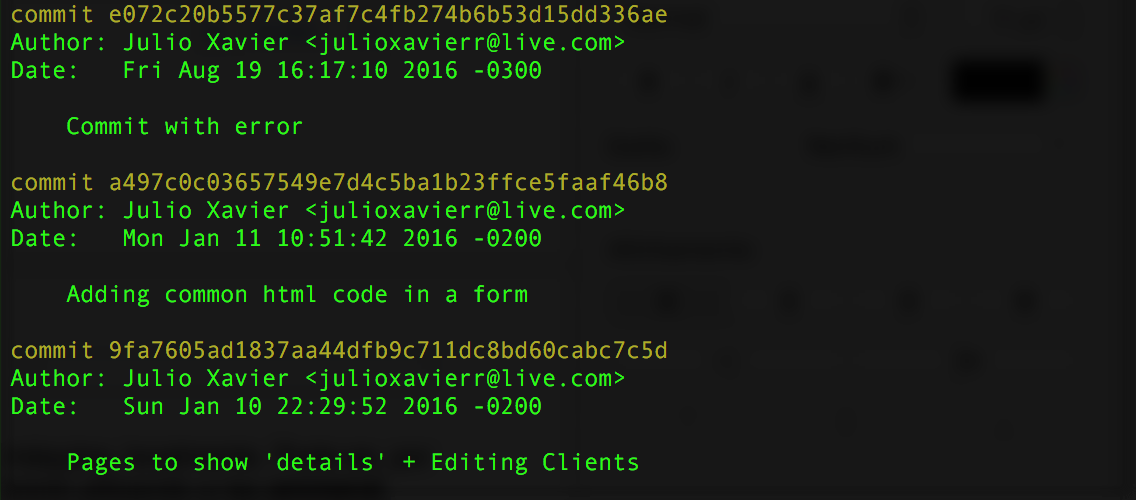
\includegraphics[width=6.25in,height=\textheight]{unidades/unidad1/../../images/git_terminal.png}

}

\caption{Git en Terminal}

\end{figure}%

Se utiliza mediante la \textbf{línea de comandos} o a través de
\textbf{interfaces gráficas} de usuario. Proporciona comandos para
realizar operaciones como:

\begin{enumerate}
\def\labelenumi{\arabic{enumi}.}
\tightlist
\item
  Inicializar un repositorio,
\item
  Realizar cambios,
\item
  Revisar historial,
\item
  Fusionar ramas,
\item
  Entre otros.
\end{enumerate}

\section{¿Para qué sirve Git? 📝}\label{para-quuxe9-sirve-git}

\begin{figure}[H]

{\centering 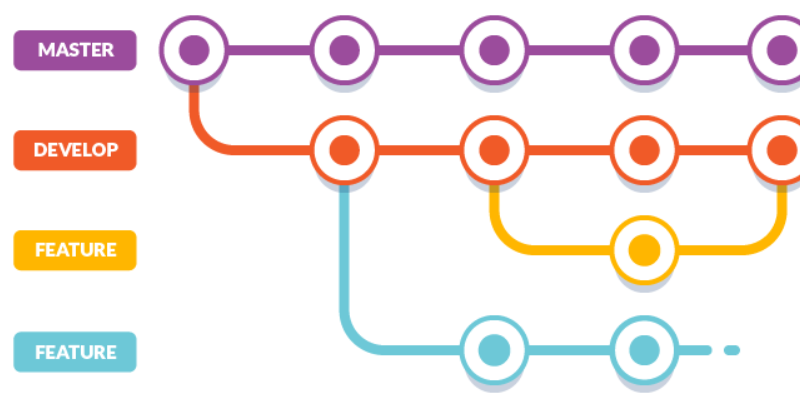
\includegraphics[width=6.25in,height=\textheight]{unidades/unidad1/../../images/seguimiento_cambios_git.png}

}

\caption{Seguimiento de Cambios con Git}

\end{figure}%

Sirve para realizar un seguimiento de los cambios en el código fuente,
coordinar el trabajo entre varios desarrolladores, revertir cambios no
deseados y mantener un historial completo de todas las modificaciones
realizadas en un proyecto.

\section{¿Por qué utilizar Git? 🤔}\label{por-quuxe9-utilizar-git}

\begin{figure}[H]

{\centering 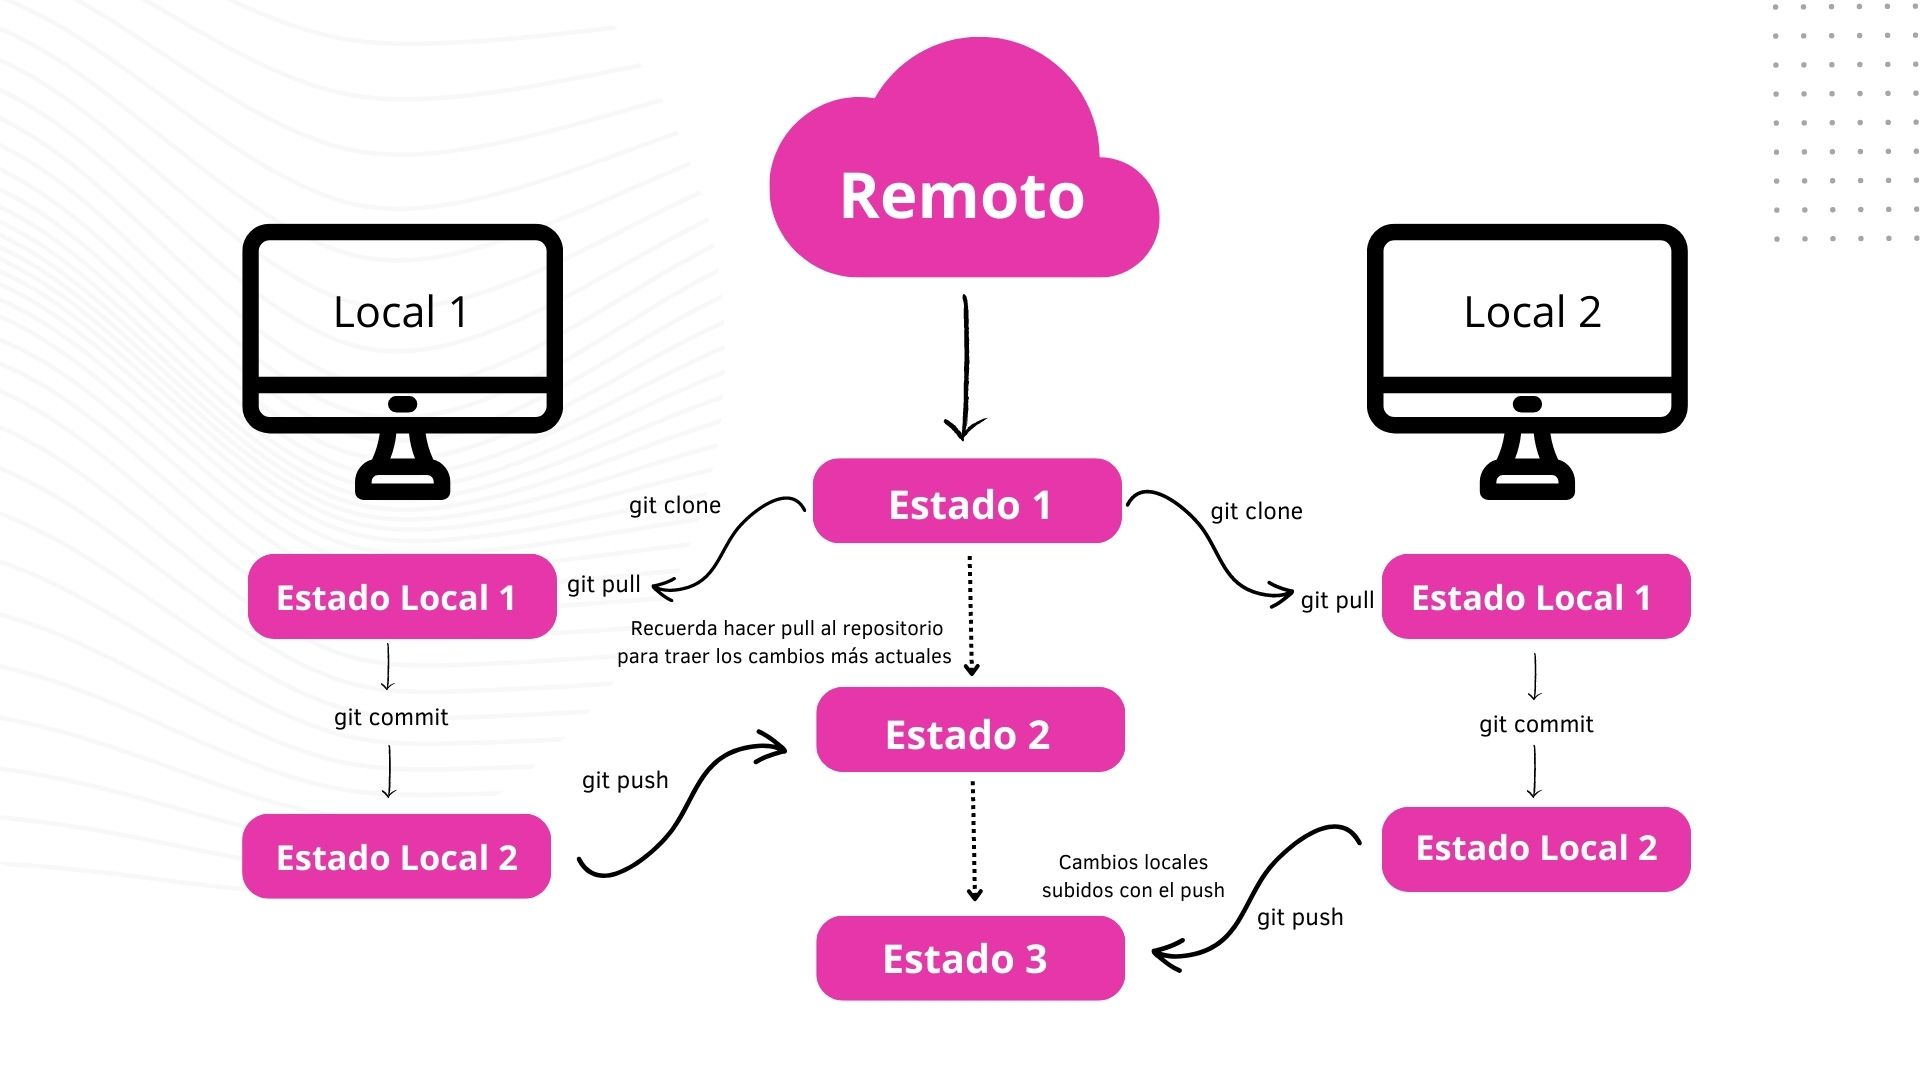
\includegraphics[width=6.25in,height=\textheight]{unidades/unidad1/../../images/ventajas_git.jpg}

}

\caption{Ventajas de Git}

\end{figure}%

Ofrece varias ventajas, como:

\begin{itemize}
\tightlist
\item
  La capacidad de trabajar de forma distribuida
\item
  La gestión eficiente de ramas para desarrollar nuevas funcionalidades
\item
  Corregir errores sin afectar la rama principal
\item
  La posibilidad de colaborar de forma efectiva con otros
  desarrolladores.
\end{itemize}

\section{¿Dónde puedo utilizar Git?
🌐}\label{duxf3nde-puedo-utilizar-git}

\begin{figure}[H]

{\centering 
\includegraphics[width=6.25in,height=\textheight]{unidades/unidad1/../../images/sistemas_operativos_git.png}

}

\caption{Git en Diferentes Sistemas Operativos}

\end{figure}%

Puede ser utilizado en cualquier sistema operativo, incluyendo Windows,
macOS y Linux. Además, es compatible con una amplia variedad de
plataformas de alojamiento de repositorios, siendo GitHub una de las más
populares.

\section{Pasos Básicos 📝}\label{pasos-buxe1sicos}

\begin{tcolorbox}[enhanced jigsaw, breakable, titlerule=0mm, colframe=quarto-callout-tip-color-frame, left=2mm, opacityback=0, rightrule=.15mm, colback=white, opacitybacktitle=0.6, title=\textcolor{quarto-callout-tip-color}{\faLightbulb}\hspace{0.5em}{Tip}, toprule=.15mm, bottomtitle=1mm, leftrule=.75mm, colbacktitle=quarto-callout-tip-color!10!white, toptitle=1mm, coltitle=black, arc=.35mm, bottomrule=.15mm]

Es recomendable tomar en cuenta una herramienta para la edición de
código, como Visual Studio Code, Sublime Text o Atom, para trabajar con
Git y GitHub de manera eficiente.

\end{tcolorbox}

\section{Instalación de Visual Studio Code
📥}\label{instalaciuxf3n-de-visual-studio-code}

\begin{figure}[H]

{\centering 
\includegraphics[width=6.25in,height=\textheight]{unidades/unidad1/../../images/vscode.png}

}

\caption{Visual Studio Code}

\end{figure}%

Si aún no tienes Visual Studio Code instalado, puedes descargarlo desde
\url{https://code.visualstudio.com/download}. Es una herramienta
gratuita y de código abierto que proporciona una interfaz amigable para
trabajar con Git y GitHub.

A continuación se presentan los pasos básicos para utilizar Git y GitHub
en un proyecto de software.

\subsection{Descarga e Instalación de Git
📥}\label{descarga-e-instalaciuxf3n-de-git}

\begin{figure}[H]

{\centering 
\includegraphics[width=6.25in,height=\textheight]{unidades/unidad1/../../images/website-git.png}

}

\caption{Git}

\end{figure}%

\begin{enumerate}
\def\labelenumi{\arabic{enumi}.}
\tightlist
\item
  Visita el sitio web oficial de Git en
  \url{https://git-scm.com/downloads}.
\item
  Descarga el instalador adecuado para tu sistema operativo y sigue las
  instrucciones de instalación.
\end{enumerate}

\subsection{Configuración 🛠️}\label{configuraciuxf3n}

\begin{figure}[H]

{\centering 
\includegraphics[width=6.25in,height=\textheight]{unidades/unidad1/../../images/git_config.png}

}

\caption{Configuración de Git}

\end{figure}%

Una vez instalado Git, es necesario configurar tu nombre de usuario y
dirección de correo electrónico. Esto se puede hacer mediante los
siguientes comandos:

\begin{Shaded}
\begin{Highlighting}[]
\FunctionTok{git}\NormalTok{ config }\AttributeTok{{-}{-}global}\NormalTok{ user.name }\StringTok{"Tu Nombre"}
\FunctionTok{git}\NormalTok{ config }\AttributeTok{{-}{-}global}\NormalTok{ user.email }\StringTok{"tu@email.com"}
\end{Highlighting}
\end{Shaded}

\subsection{Creación de un Repositorio ``helloWorld'' en Python
🐍}\label{creaciuxf3n-de-un-repositorio-helloworld-en-python}

\begin{itemize}
\tightlist
\item
  Crea una nueva carpeta para tu proyecto y ábrela en Visual Studio
  Code.
\item
  Crea un archivo Python llamado \textbf{hello\_world.py} y escribe el
  siguiente código:
\end{itemize}

\begin{Shaded}
\begin{Highlighting}[]
\KeywordTok{def}\NormalTok{ welcome\_message():}
\NormalTok{    name }\OperatorTok{=} \BuiltInTok{input}\NormalTok{(}\StringTok{"Ingrese su nombre: "}\NormalTok{)}
    \BuiltInTok{print}\NormalTok{(}\StringTok{"Bienvenio,"}\NormalTok{, name, }\StringTok{"al curso de Django y React!"}\NormalTok{)}

\ControlFlowTok{if} \VariableTok{\_\_name\_\_} \OperatorTok{==} \StringTok{"\_\_main\_\_"}\NormalTok{:}
\NormalTok{    welcome\_message()}
\end{Highlighting}
\end{Shaded}

\begin{itemize}
\tightlist
\item
  Guarda el archivo y abre una terminal en Visual Studio Code.
\item
  Inicializa un repositorio Git en la carpeta de tu proyecto con el
  siguiente comando:
\end{itemize}

\begin{Shaded}
\begin{Highlighting}[]
\FunctionTok{git}\NormalTok{ init}
\end{Highlighting}
\end{Shaded}

\begin{itemize}
\tightlist
\item
  Añade el archivo al área de preparación con:
\end{itemize}

\begin{Shaded}
\begin{Highlighting}[]
\FunctionTok{git}\NormalTok{ add hello\_world.py}
\end{Highlighting}
\end{Shaded}

\begin{itemize}
\tightlist
\item
  Realiza un commit de los cambios con un mensaje descriptivo:
\end{itemize}

\begin{Shaded}
\begin{Highlighting}[]
\FunctionTok{git}\NormalTok{ commit }\AttributeTok{{-}m} \StringTok{"Añadir archivo hello\_world.py"}
\end{Highlighting}
\end{Shaded}

\subsection{Comandos Básicos de Git
📝}\label{comandos-buxe1sicos-de-git}

\begin{itemize}
\tightlist
\item
  \textbf{git init:} Inicializa un nuevo repositorio Git.
\item
  \textbf{git add :} Añade un archivo al área de preparación.
\item
  \textbf{git commit -m ``''}: Realiza un commit de los cambios con un
  mensaje descriptivo.
\item
  \textbf{git push:} Sube los cambios al repositorio remoto.
\item
  \textbf{git pull:} Descarga cambios del repositorio remoto.
\item
  \textbf{git branch:} Lista las ramas disponibles.
\item
  \textbf{git checkout :} Cambia a una rama específica.
\item
  \textbf{git merge :} Fusiona una rama con la rama actual.
\item
  \textbf{git reset :} Descarta los cambios en un archivo.
\item
  \textbf{git diff:} Muestra las diferencias entre versiones.
\end{itemize}

\subsection{Estados en Git 📊}\label{estados-en-git}

\begin{itemize}
\tightlist
\item
  \textbf{Local:} Representa los cambios que realizas en tu repositorio
  local antes de hacer un commit. Estos cambios están únicamente en tu
  máquina.
\item
  \textbf{Staging:} Indica los cambios que has añadido al área de
  preparación con el comando \texttt{git\ add}. Estos cambios están
  listos para ser confirmados en el próximo commit.
\item
  \textbf{Commit:} Son los cambios que has confirmado en tu repositorio
  local con el comando \texttt{git\ commit}. Estos cambios se han
  guardado de manera permanente en tu repositorio local.
\item
  \textbf{Server:} Son los cambios que has subido al repositorio remoto
  con el comando \texttt{git\ push}. Estos cambios están disponibles
  para otros colaboradores del proyecto.
\end{itemize}

\begin{center}\rule{0.5\linewidth}{0.5pt}\end{center}

\chapter{Tutorial: Moviendo Cambios entre Estados en Git
📝}\label{tutorial-moviendo-cambios-entre-estados-en-git}

\section{Introducción}\label{introducciuxf3n}

En este tutorial, aprenderemos a utilizar Git para gestionar cambios en
nuestro proyecto y moverlos entre diferentes estados. Utilizaremos un
ejemplo práctico para comprender mejor estos conceptos.

\begin{Shaded}
\begin{Highlighting}[]
\KeywordTok{def}\NormalTok{ welcome\_message():}
\NormalTok{    name }\OperatorTok{=} \BuiltInTok{input}\NormalTok{(}\StringTok{"Ingrese su nombre: "}\NormalTok{)}
    \BuiltInTok{print}\NormalTok{(}\StringTok{"Bienvenio,"}\NormalTok{, name, }\StringTok{"al curso de Django y React!"}\NormalTok{)}

\ControlFlowTok{if} \VariableTok{\_\_name\_\_} \OperatorTok{==} \StringTok{"\_\_main\_\_"}\NormalTok{:}
\NormalTok{    welcome\_message()}
\end{Highlighting}
\end{Shaded}

\section{Sección 1: Modificar Archivos en el
Repositorio}\label{secciuxf3n-1-modificar-archivos-en-el-repositorio}

En esta sección, aprenderemos cómo realizar cambios en nuestros archivos
y reflejarlos en Git.

\section{Mover Cambios de Local a
Staging:}\label{mover-cambios-de-local-a-staging}

\begin{enumerate}
\def\labelenumi{\arabic{enumi}.}
\tightlist
\item
  Abre el archivo \textbf{hello\_world.py} en Visual Studio Code.
\item
  Modifica el mensaje de bienvenida a ``Bienvenido'' en lugar de
  ``Bienvenio''.
\item
  Guarda los cambios y abre una terminal en Visual Studio Code.
\end{enumerate}

Hemos corregido un error en nuestro archivo y queremos reflejarlo en
Git.

\begin{Shaded}
\begin{Highlighting}[]
\ExtensionTok{def}\NormalTok{ welcome\_message}\ErrorTok{(}\KeywordTok{)}\BuiltInTok{:}
    \ExtensionTok{name}\NormalTok{ = input}\ErrorTok{(}\StringTok{"Ingrese su nombre: "}\KeywordTok{)}
    \ExtensionTok{print}\ErrorTok{(}\StringTok{"Bienvenido,"}\ExtensionTok{,}\NormalTok{ name, }\StringTok{"al curso de Django y React!"}\KeywordTok{)}

\ControlFlowTok{if} \ExtensionTok{\_\_name\_\_}\NormalTok{ == }\StringTok{"\_\_main\_\_"}\NormalTok{:}
    \FunctionTok{welcome\_message()}
\end{Highlighting}
\end{Shaded}

\section{Agregar Cambios de Local a
Staging:}\label{agregar-cambios-de-local-a-staging}

\begin{Shaded}
\begin{Highlighting}[]
\FunctionTok{git}\NormalTok{ add hello\_world.py}
\end{Highlighting}
\end{Shaded}

Hemos añadido los cambios al área de preparación y están listos para ser
confirmados en el próximo commit.

\section{Sección 2: Confirmar Cambios en un
Commit}\label{secciuxf3n-2-confirmar-cambios-en-un-commit}

En esta sección, aprenderemos cómo confirmar los cambios en un commit y
guardarlos de manera permanente en nuestro repositorio.

\section{Mover Cambios de Staging a
Commit:}\label{mover-cambios-de-staging-a-commit}

\begin{Shaded}
\begin{Highlighting}[]
\FunctionTok{git}\NormalTok{ commit }\AttributeTok{{-}m} \StringTok{"Corregir mensaje de bienvenida"}
\end{Highlighting}
\end{Shaded}

Hemos confirmado los cambios en un commit con un mensaje descriptivo.

\section{Sección 3: Creación y Fusión de
Ramas}\label{secciuxf3n-3-creaciuxf3n-y-fusiuxf3n-de-ramas}

En esta sección, aprenderemos cómo crear y fusionar ramas en Git para
desarrollar nuevas funcionalidades de forma aislada.

\section{Crear una Nueva Rama:}\label{crear-una-nueva-rama}

\begin{Shaded}
\begin{Highlighting}[]
\FunctionTok{git}\NormalTok{ branch feature}
\end{Highlighting}
\end{Shaded}

Hemos creado una nueva rama llamada ``feature'' para desarrollar una
nueva funcionalidad.

\section{Implementar Funcionalidades en la
Rama:}\label{implementar-funcionalidades-en-la-rama}

\begin{enumerate}
\def\labelenumi{\arabic{enumi}.}
\tightlist
\item
  Abre el archivo \textbf{hello\_world.py} en Visual Studio Code.
\item
  Añade una nueva función para mostrar un mensaje de despedida.
\item
  Guarda los cambios y abre una terminal en Visual Studio Code.
\item
  Añade los cambios al área de preparación y confírmalos en un commit.
\item
  Cambia a la rama principal con \texttt{git\ checkout\ main}.
\end{enumerate}

\section{Fusionar Ramas con la Rama
Principal:}\label{fusionar-ramas-con-la-rama-principal}

\begin{Shaded}
\begin{Highlighting}[]
\FunctionTok{git}\NormalTok{ merge feature}
\end{Highlighting}
\end{Shaded}

Hemos fusionado la rama ``feature'' con la rama principal y añadido la
nueva funcionalidad al proyecto.

\section{Sección 4: Revertir Cambios en un
Archivo}\label{secciuxf3n-4-revertir-cambios-en-un-archivo}

En esta sección, aprenderemos cómo revertir cambios en un archivo y
deshacerlos en Git.

\section{Revertir Cambios en un
Archivo:}\label{revertir-cambios-en-un-archivo}

\begin{Shaded}
\begin{Highlighting}[]
\FunctionTok{git}\NormalTok{ reset hello\_world.py}
\end{Highlighting}
\end{Shaded}

Hemos revertido los cambios en el archivo \textbf{hello\_world.py} y
deshecho las modificaciones realizadas.

\section{Conclusión}\label{conclusiuxf3n}

En este tutorial, hemos aprendido a gestionar cambios en nuestro
proyecto y moverlos entre diferentes estados en Git. Estos conceptos son
fundamentales para trabajar de forma eficiente en proyectos de software
y colaborar con otros desarrolladores.

\chapter{Asignación}\label{asignaciuxf3n}

\href{https://classroom.github.com/a/o-qydr2W}{Hello World!}

Este proyecto de ejemplo está escrito en Python y se prueba con pytest.

\textbf{La Asignación}

Las pruebas están fallando en este momento porque el método no está
devolviendo la cadena correcta. Corrige el código del archivo
\textbf{hello.py} para que las pruebas sean exitosas, debe devolver la
cadena correcta \textbf{``Hello World!''}x

El comando de ejecución del test es:

\begin{Shaded}
\begin{Highlighting}[]
\ExtensionTok{pytest}\NormalTok{ test\_hello.py}
\end{Highlighting}
\end{Shaded}

¡Mucha suerte!

\chapter{GitHub Classroom 📒}\label{github-classroom}

\begin{figure}[H]

{\centering 
\includegraphics[width=1.04167in,height=\textheight]{unidades/unidad1/../../images/github classroom.png}

}

\caption{Github Classroom}

\end{figure}%

GitHub Classroom es una herramienta poderosa que facilita la gestión de
tareas y asignaciones en GitHub, especialmente diseñada para entornos
educativos.

\section{¿Qué es GitHub Classroom? 🤔}\label{quuxe9-es-github-classroom}

\begin{figure}[H]

{\centering 
\includegraphics[width=4.16667in,height=\textheight]{unidades/unidad1/../../images/github-classroom-ventana.jpg}

}

\caption{Github Classroom Windows}

\end{figure}%

GitHub Classroom es una extensión de GitHub que permite a los profesores
crear y gestionar asignaciones utilizando repositorios de GitHub.
Proporciona una forma organizada y eficiente de distribuir tareas a los
estudiantes, recopilar y revisar su trabajo, y proporcionar
retroalimentación.

\subsection{Funcionalidades Principales
⚙️}\label{funcionalidades-principales}

\textbf{Creación de Asignaciones:} Los profesores pueden crear tareas y
asignaciones directamente desde GitHub Classroom, proporcionando
instrucciones detalladas y estableciendo criterios de evaluación.

\textbf{Distribución Automatizada:} Una vez que se crea una asignación,
GitHub Classroom genera automáticamente repositorios privados para cada
estudiante o equipo, basándose en una plantilla predefinida.

\textbf{Seguimiento de Progreso:} Los profesores pueden realizar un
seguimiento del progreso de los estudiantes y revisar sus contribuciones
a través de solicitudes de extracción (pull requests) y comentarios en
el código.

\textbf{Revisión y Retroalimentación:} Los estudiantes envían sus
trabajos a través de solicitudes de extracción, lo que permite a los
profesores revisar y proporcionar retroalimentación específica sobre su
código.

\section{Ejemplo Práctico}\label{ejemplo-pruxe1ctico}

\subsection{Creación de una Asignación en GitHub Classroom
📒}\label{creaciuxf3n-de-una-asignaciuxf3n-en-github-classroom}

\textbf{Iniciar Sesión:} Ingresa a GitHub Classroom con tu cuenta de
GitHub y selecciona la opción para crear una nueva asignación.

\begin{center}
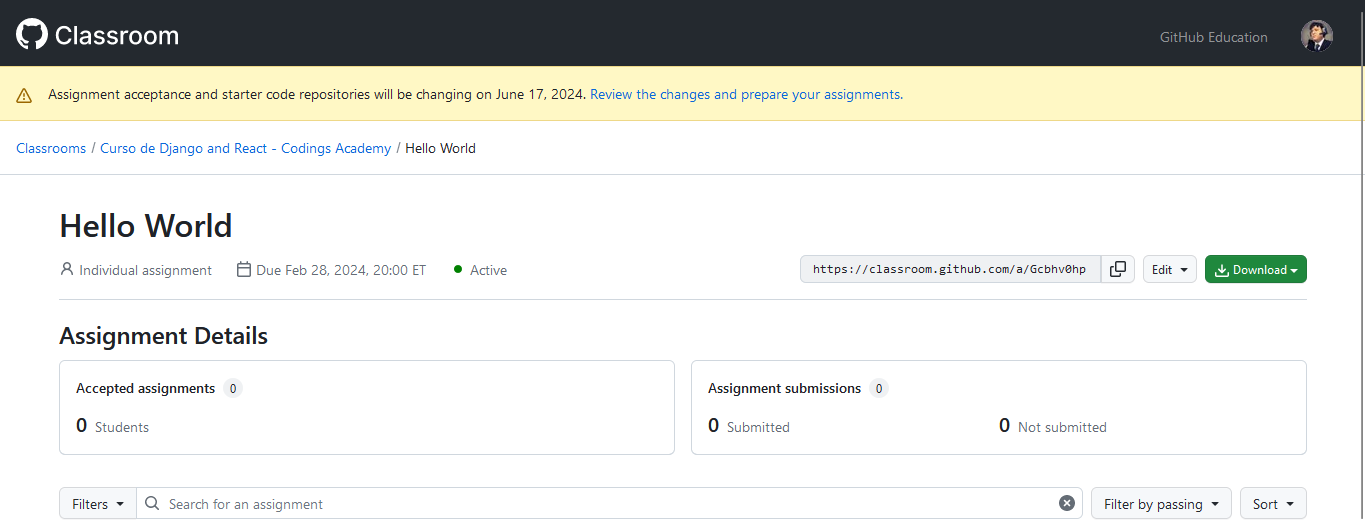
\includegraphics{unidades/unidad1/images/paste-2.png}
\end{center}

\textbf{Definir la Tarea:} Proporciona instrucciones claras y detalladas
sobre la tarea, incluyendo cualquier código base o recursos necesarios.
Establece los criterios de evaluación para guiar a los estudiantes.

\begin{center}
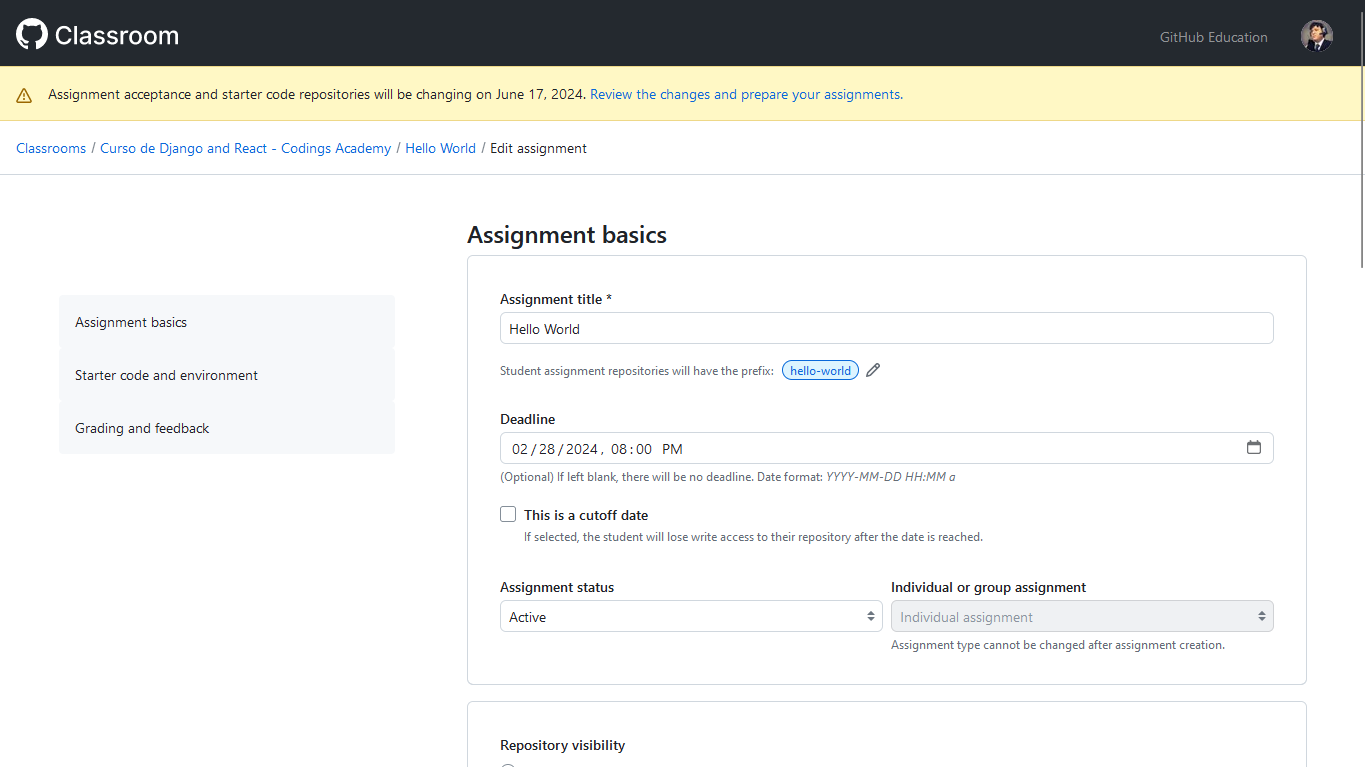
\includegraphics{unidades/unidad1/images/paste-1.png}
\end{center}

\textbf{Configurar la Plantilla:} Selecciona una plantilla de
repositorio existente o crea una nueva plantilla que servirá como base
para los repositorios de los estudiantes.

\begin{center}
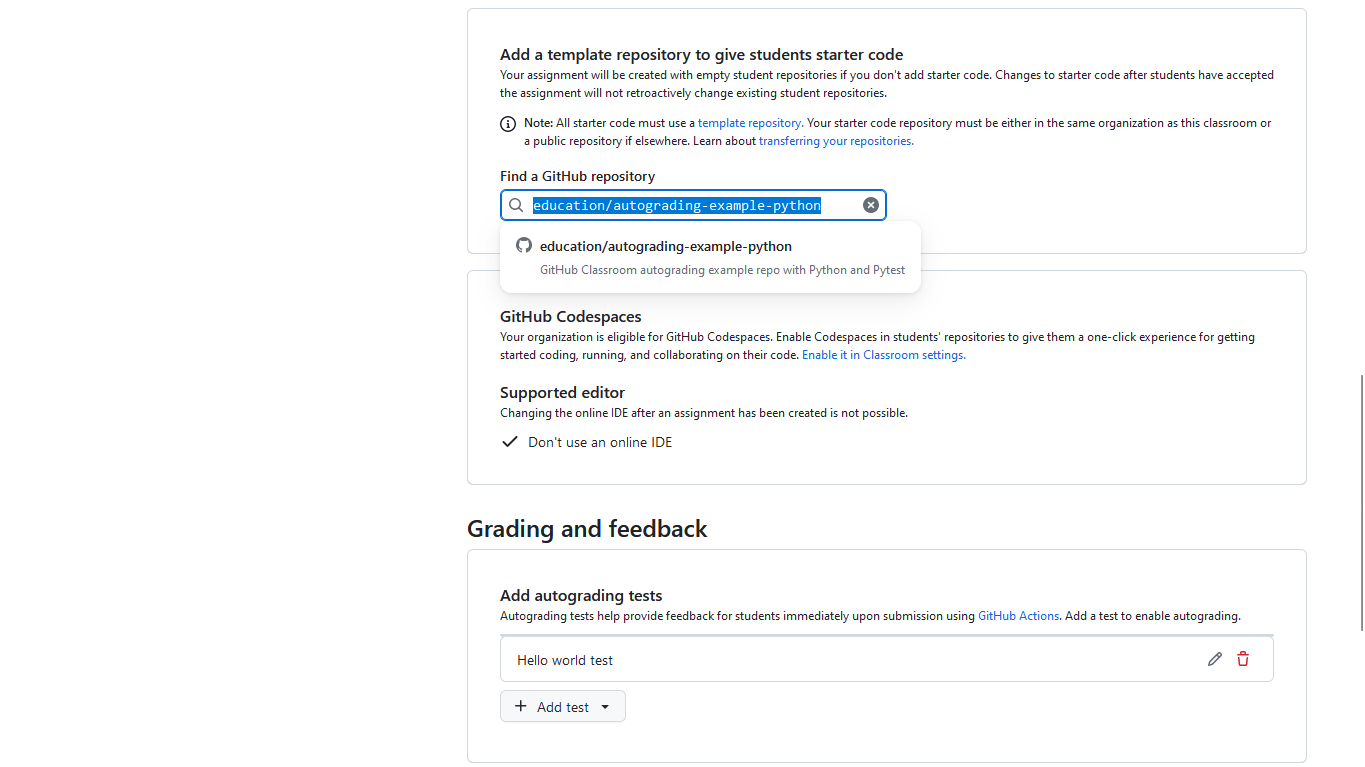
\includegraphics{unidades/unidad1/images/paste-3.png}
\end{center}

\textbf{Distribuir la Asignación:} Una vez configurada la asignación,
comparte el enlace generado con tus estudiantes para que puedan acceder
a sus repositorios privados.

\begin{center}

\includegraphics{unidades/unidad1/images/paste-4.png}
\end{center}

\section{Trabajo de los Estudiantes
🧑‍💻}\label{trabajo-de-los-estudiantes}

\textbf{Aceptar la Asignación:} Los estudiantes reciben el enlace de la
asignación y aceptan la tarea, lo que les permite crear un repositorio
privado basado en la plantilla proporcionada.

\begin{center}
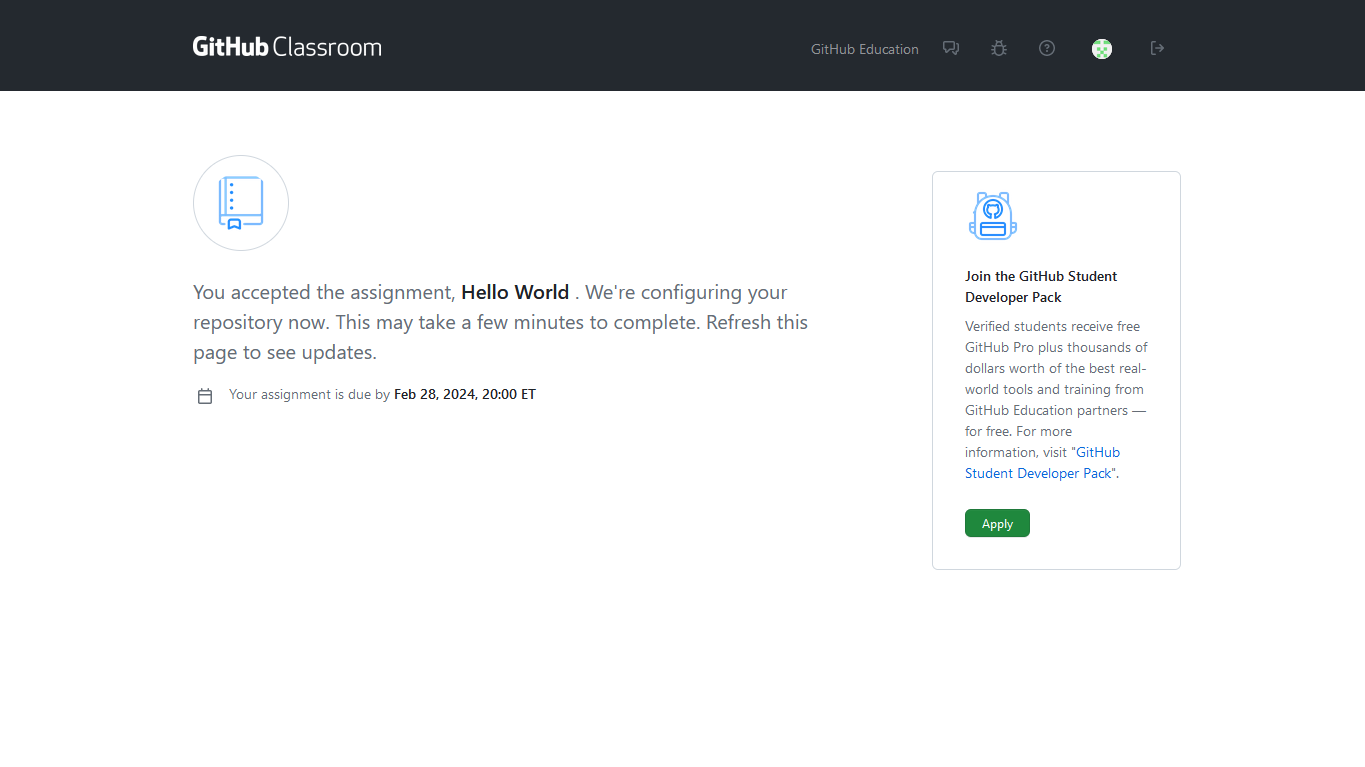
\includegraphics{unidades/unidad1/images/paste-6.png}
\end{center}

\textbf{Actualizar el Navegador:} Los estudiantes actualizan su
navegador para ver el nuevo repositorio creado en su cuenta de GitHub.

\begin{center}
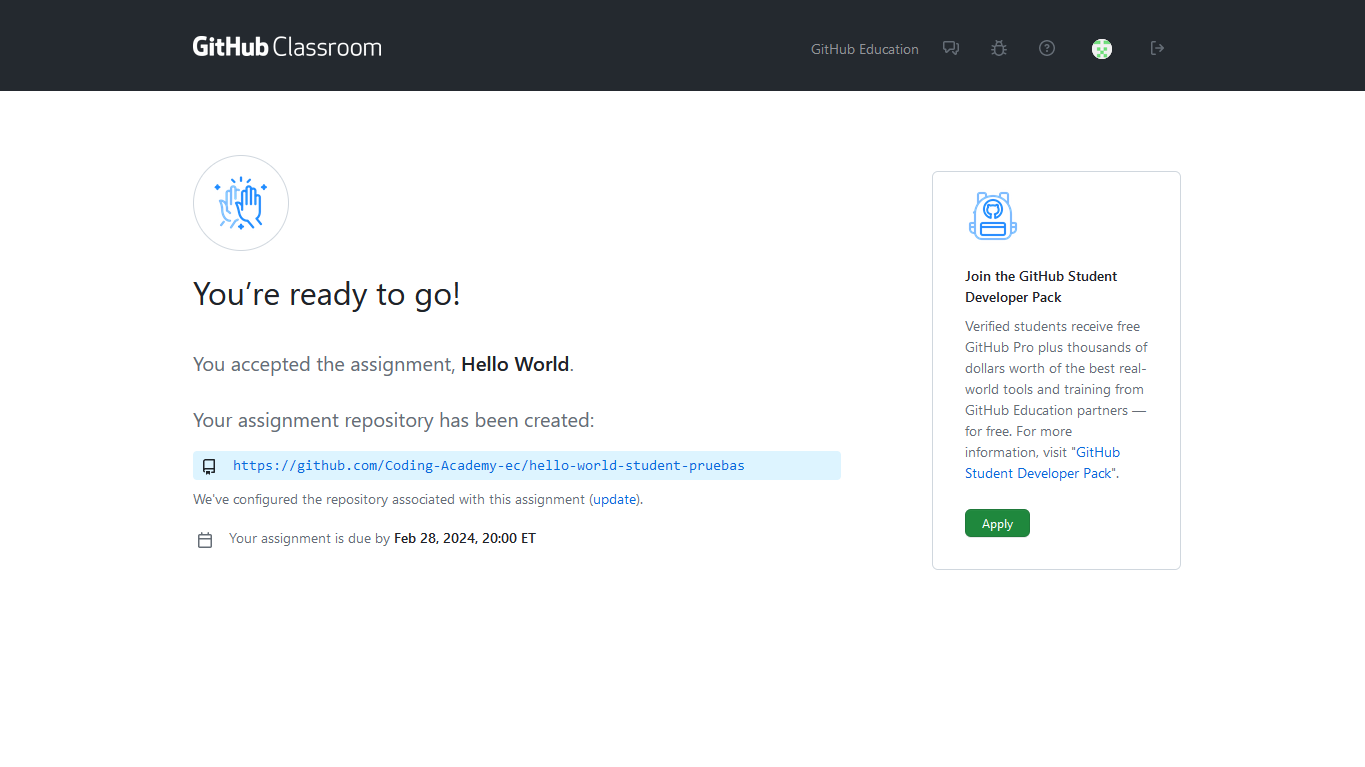
\includegraphics{unidades/unidad1/images/paste-8.png}
\end{center}

\textbf{Clonar el Repositorio:} Los estudiantes clonan el repositorio
asignado en su computadora local utilizando el enlace proporcionado.

\begin{center}
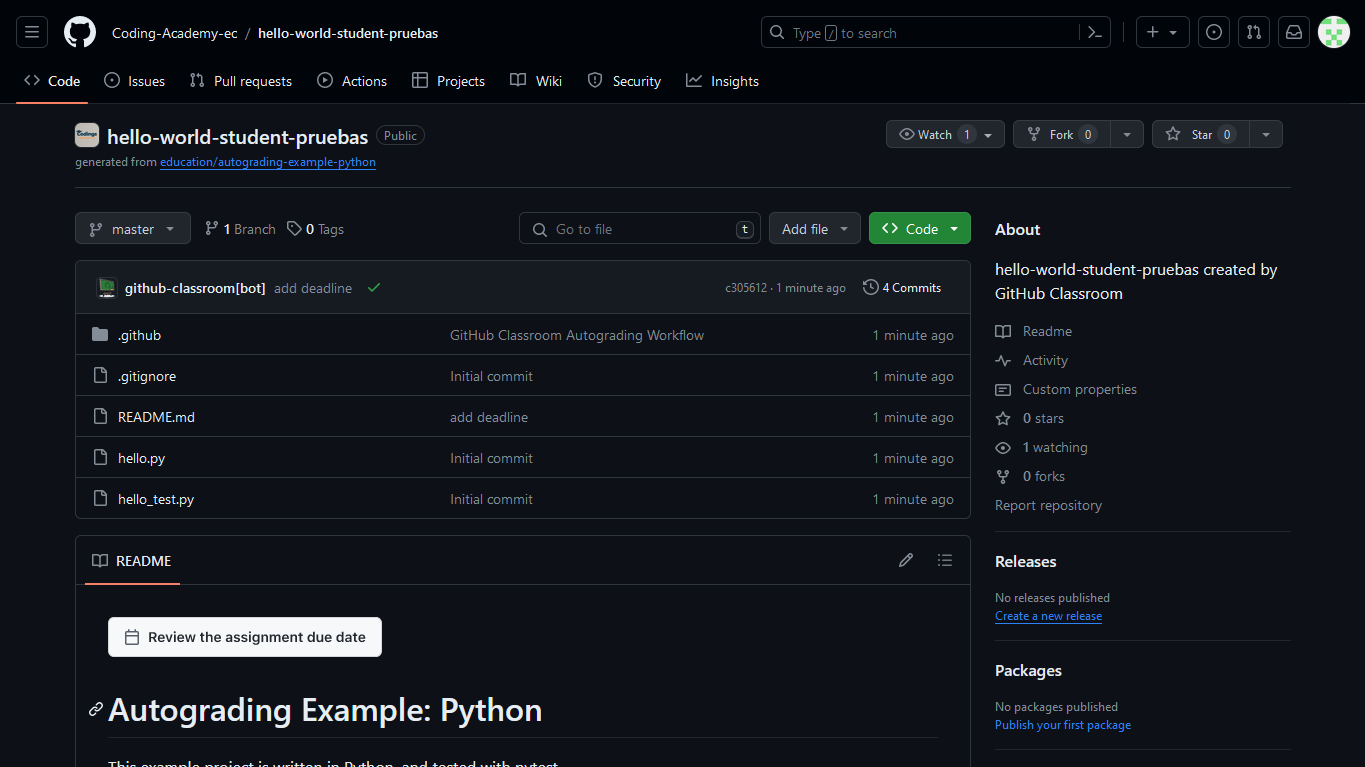
\includegraphics{unidades/unidad1/images/paste-9.png}
\end{center}

Utilizar el comando git clone: Aplique el comando git clone para clonar
el repositorio en su computadora local.

\begin{Shaded}
\begin{Highlighting}[]
\FunctionTok{git}\NormalTok{ clone }\OperatorTok{\textless{}}\NormalTok{enlace{-}del{-}repositorio}\OperatorTok{\textgreater{}}
\end{Highlighting}
\end{Shaded}

\begin{center}
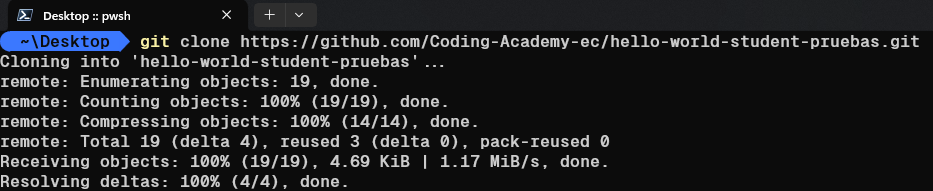
\includegraphics{unidades/unidad1/images/paste-10.png}
\end{center}

\textbf{Desarrollar la Tarea:} Los estudiantes trabajan en la tarea,
realizando los cambios necesarios y realizando commits de manera regular
para mantener un historial de su trabajo.

\begin{tcolorbox}[enhanced jigsaw, breakable, titlerule=0mm, colframe=quarto-callout-tip-color-frame, left=2mm, opacityback=0, rightrule=.15mm, colback=white, opacitybacktitle=0.6, title=\textcolor{quarto-callout-tip-color}{\faLightbulb}\hspace{0.5em}{Tip}, toprule=.15mm, bottomtitle=1mm, leftrule=.75mm, colbacktitle=quarto-callout-tip-color!10!white, toptitle=1mm, coltitle=black, arc=.35mm, bottomrule=.15mm]

Puedes probar el test incorporado con el comando \texttt{pytest} en la
terminal, para verificar que el código cumple con los requerimientos

\end{tcolorbox}

\begin{Shaded}
\begin{Highlighting}[]
\ExtensionTok{pytest}
\end{Highlighting}
\end{Shaded}

Una vez desarrollado el código de acuerdo a la asignación en local
deberían pasar el o los test

\begin{center}
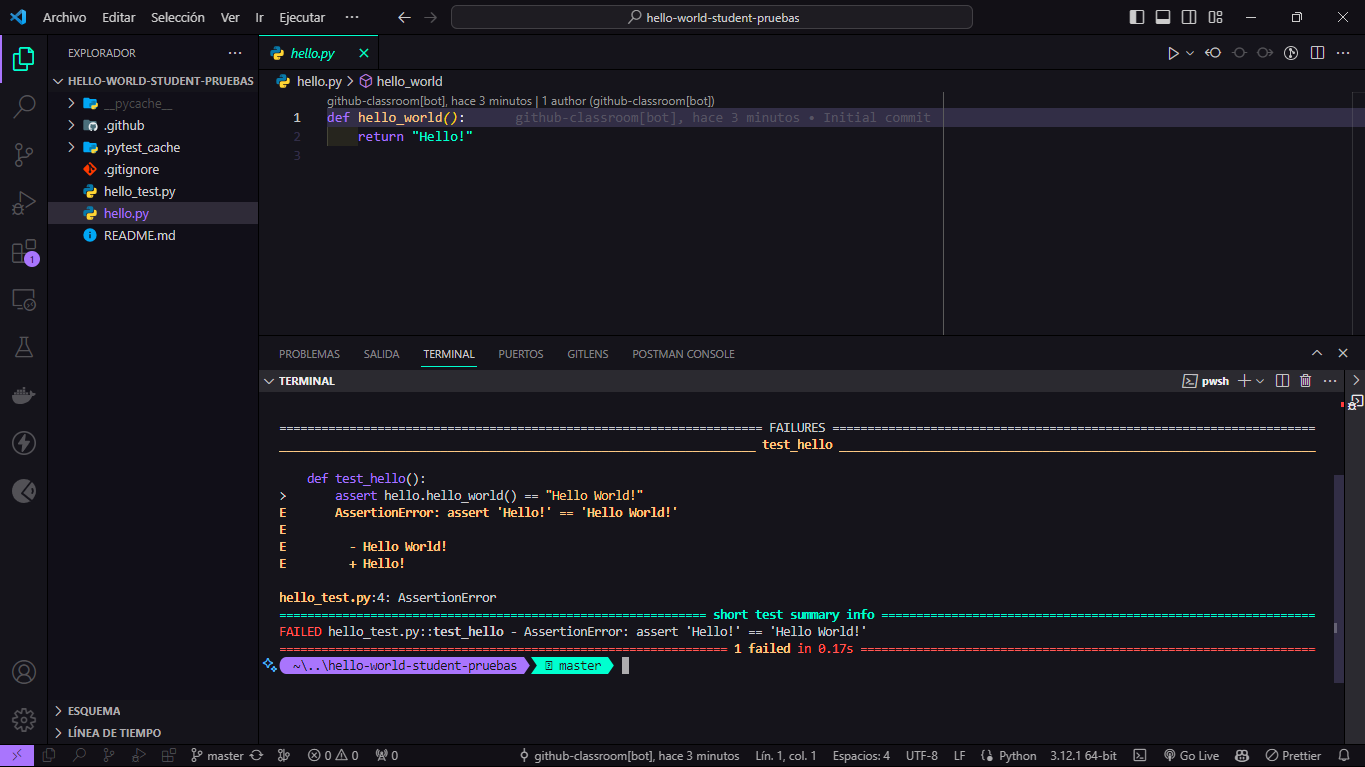
\includegraphics{unidades/unidad1/images/paste-11.png}
\end{center}

\textbf{Enviar la Solicitud de Extracción:} Una vez completada la tarea,
los estudiantes envían una solicitud de extracción desde su rama hacia
la rama principal del repositorio, solicitando la revisión del profesor.

\begin{center}
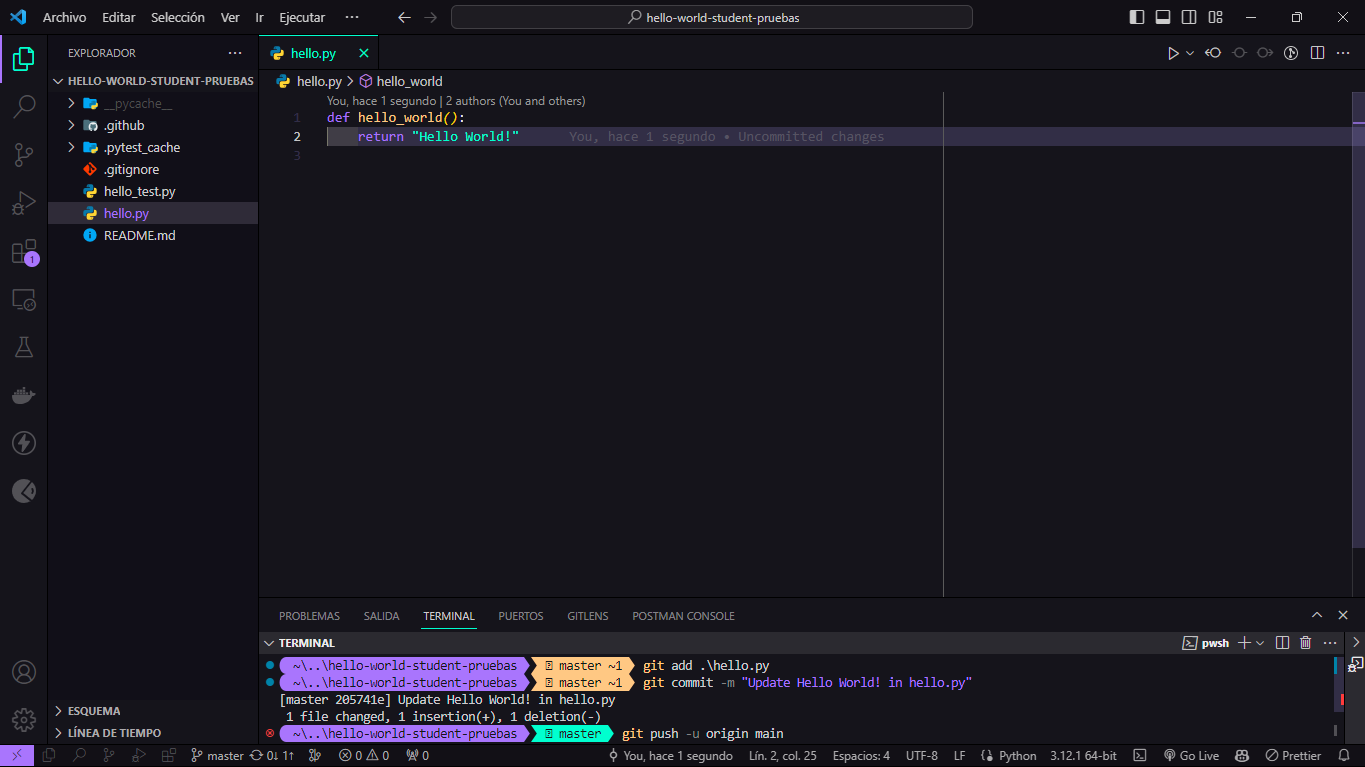
\includegraphics{unidades/unidad1/images/paste-12.png}
\end{center}

Una vez realizado el \texttt{push} se envía al respositorio principal y
se ejecutan los test en Github

\begin{tcolorbox}[enhanced jigsaw, breakable, titlerule=0mm, colframe=quarto-callout-tip-color-frame, left=2mm, opacityback=0, rightrule=.15mm, colback=white, opacitybacktitle=0.6, title=\textcolor{quarto-callout-tip-color}{\faLightbulb}\hspace{0.5em}{Tip}, toprule=.15mm, bottomtitle=1mm, leftrule=.75mm, colbacktitle=quarto-callout-tip-color!10!white, toptitle=1mm, coltitle=black, arc=.35mm, bottomrule=.15mm]

Se recomienda hacer las pruebas en local antes de enviar los cambios al
respositorio en Github

\end{tcolorbox}

\begin{center}
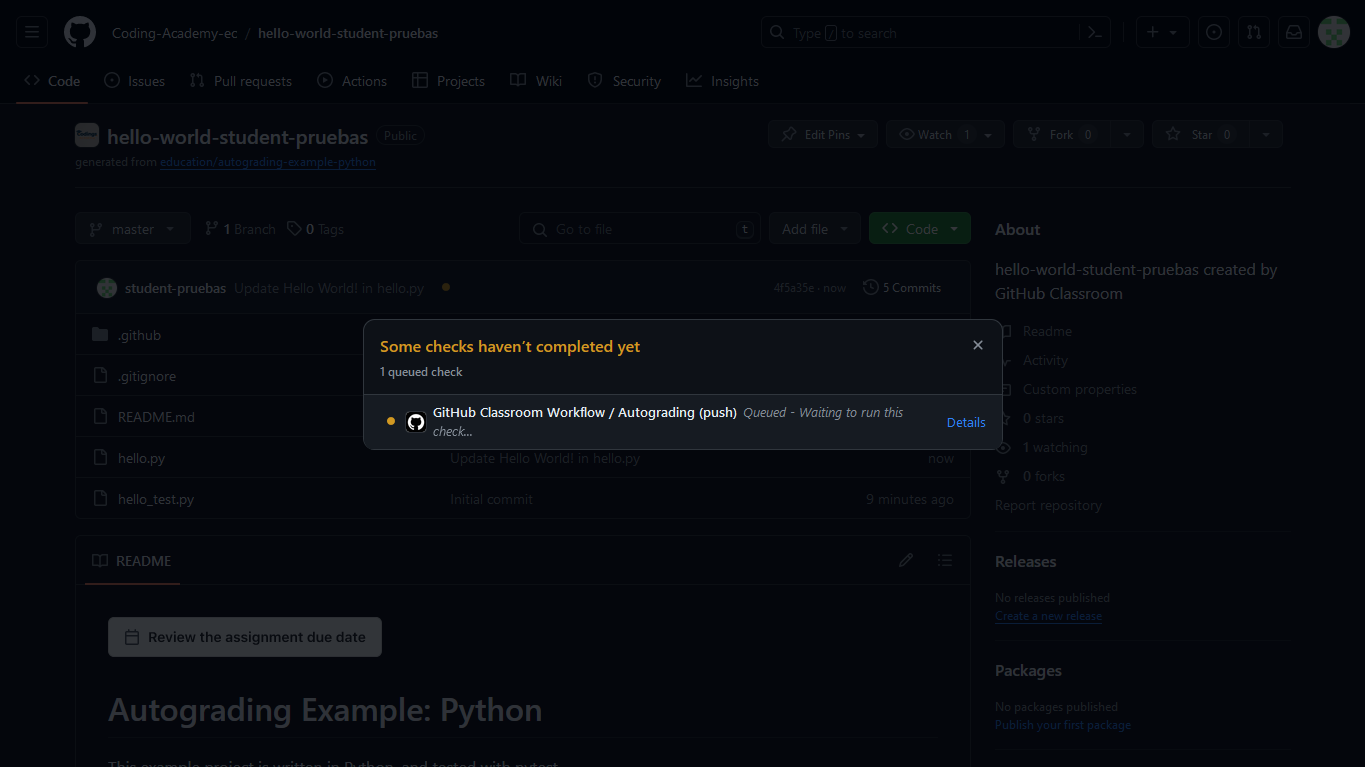
\includegraphics{unidades/unidad1/images/paste-13.png}
\end{center}

Este Action lo que hace es evaluar los cambios realizados

\begin{center}
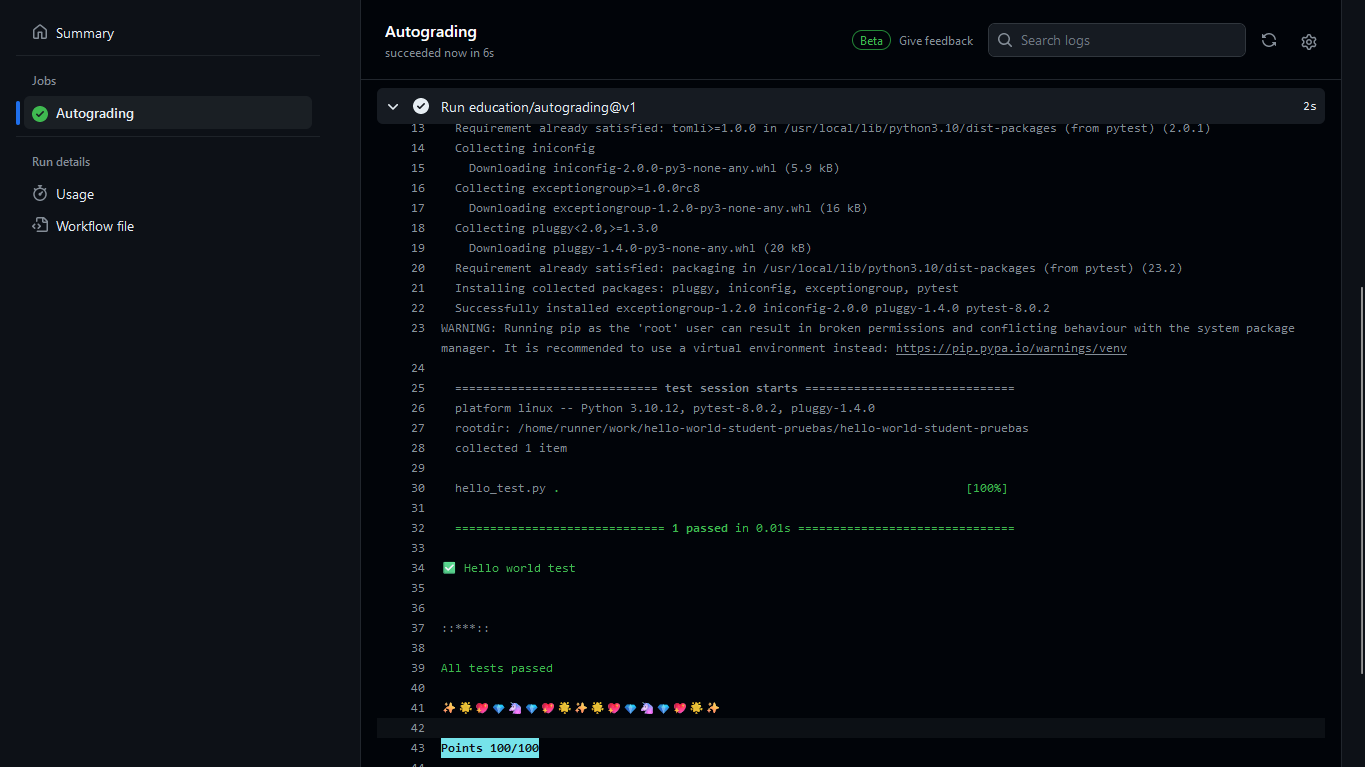
\includegraphics{unidades/unidad1/images/paste-14.png}
\end{center}

\begin{tcolorbox}[enhanced jigsaw, breakable, titlerule=0mm, colframe=quarto-callout-tip-color-frame, left=2mm, opacityback=0, rightrule=.15mm, colback=white, opacitybacktitle=0.6, title=\textcolor{quarto-callout-tip-color}{\faLightbulb}\hspace{0.5em}{Tip}, toprule=.15mm, bottomtitle=1mm, leftrule=.75mm, colbacktitle=quarto-callout-tip-color!10!white, toptitle=1mm, coltitle=black, arc=.35mm, bottomrule=.15mm]

Se recomienda hacer las pruebas en local antes de enviar los cambios al
respositorio en Github

\end{tcolorbox}

\textbf{Revisión y Retroalimentación:} Los profesores revisan las
solicitudes de extracción, proporcionan comentarios sobre el código y
evalúan el trabajo de los estudiantes según los criterios establecidos.

\begin{center}
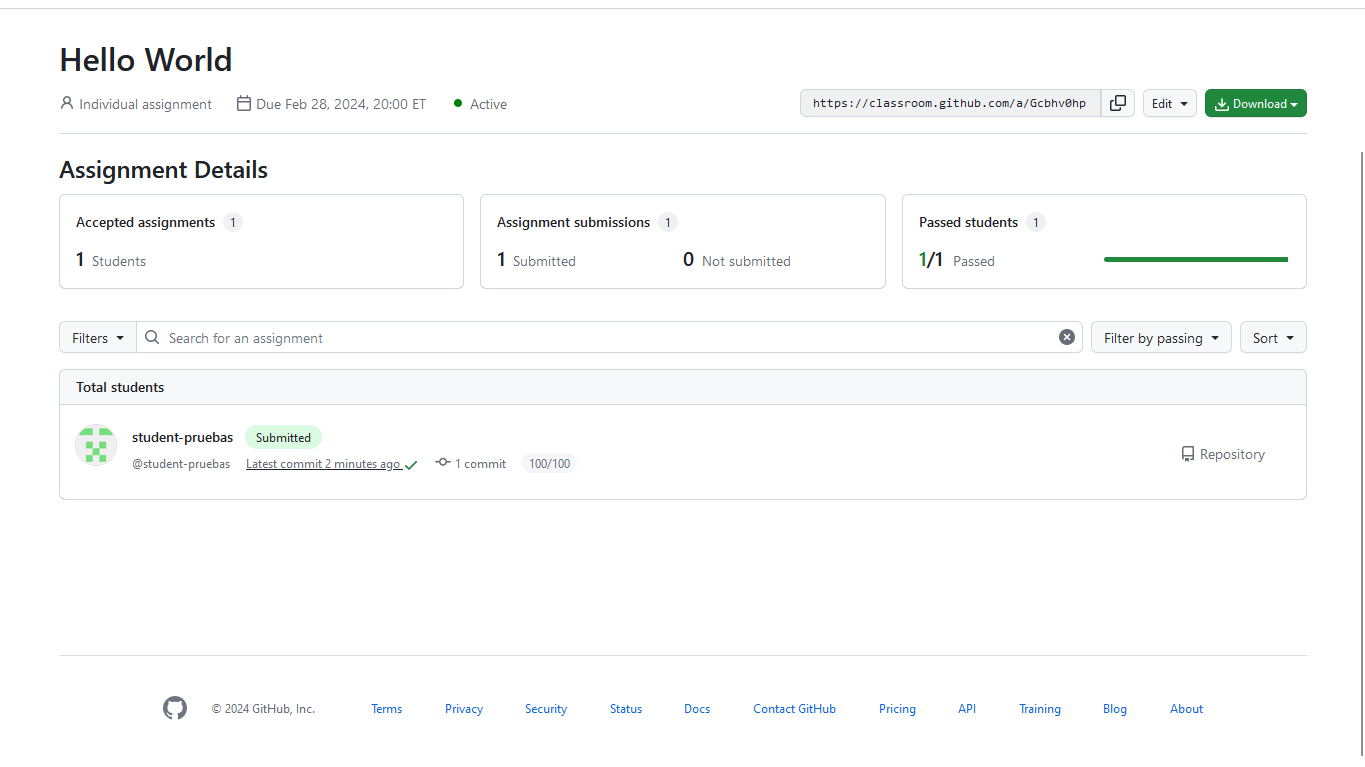
\includegraphics{unidades/unidad1/images/paste-15.png}
\end{center}

\begin{tcolorbox}[enhanced jigsaw, breakable, titlerule=0mm, colframe=quarto-callout-tip-color-frame, left=2mm, opacityback=0, rightrule=.15mm, colback=white, opacitybacktitle=0.6, title=\textcolor{quarto-callout-tip-color}{\faLightbulb}\hspace{0.5em}{Tip}, toprule=.15mm, bottomtitle=1mm, leftrule=.75mm, colbacktitle=quarto-callout-tip-color!10!white, toptitle=1mm, coltitle=black, arc=.35mm, bottomrule=.15mm]

\textbf{GitHub Classroom} ofrece una manera eficiente y organizada de
administrar tareas y asignaciones en entornos educativos, fomentando la
colaboración, el aprendizaje y la retroalimentación efectiva entre
profesores y estudiantes.

\end{tcolorbox}

\chapter{Docker 🐋}\label{docker}

\begin{figure}[H]

{\centering 
\includegraphics[width=1.04167in,height=\textheight]{unidades/unidad1/../../images/docker-logo.png}

}

\caption{Docker}

\end{figure}%

Docker es una plataforma de código abierto que permite a los
desarrolladores empaquetar, distribuir y ejecutar aplicaciones en
contenedores. Los contenedores son entornos ligeros y portátiles que
incluyen todo lo necesario para ejecutar una aplicación de forma
consistente en cualquier entorno.

\chapter{Conceptos Básicos de Docker
📒}\label{conceptos-buxe1sicos-de-docker}

\section{Imagen}\label{imagen}

\begin{Shaded}
\begin{Highlighting}[]
\ExtensionTok{docker}\NormalTok{ pull python:3.9{-}slim}
\end{Highlighting}
\end{Shaded}

Una imagen de Docker es un paquete de software ligero y portátil que
incluye todo lo necesario para ejecutar una aplicación, incluidos el
código, las bibliotecas y las dependencias. Las imágenes se utilizan
como plantillas para crear contenedores.

\section{Contenedor 📦}\label{contenedor}

\begin{Shaded}
\begin{Highlighting}[]
\ExtensionTok{docker}\NormalTok{ run }\AttributeTok{{-}d} \AttributeTok{{-}p}\NormalTok{ 5000:5000 myapp}
\end{Highlighting}
\end{Shaded}

Un contenedor de Docker es una instancia en tiempo de ejecución de una
imagen de Docker. Los contenedores son entornos aislados que ejecutan
aplicaciones de forma independiente y comparten recursos del sistema
operativo subyacente. Cada contenedor está aislado del entorno de host y
otros contenedores, lo que garantiza la consistencia y la portabilidad
de las aplicaciones.

\section{Dockerfile 📘}\label{dockerfile}

\begin{Shaded}
\begin{Highlighting}[]
\CommentTok{\# Dockerfile}
\CommentTok{\# Define la imagen base}
\KeywordTok{FROM}\NormalTok{ python:3.9{-}slim}

\CommentTok{\# Instala las dependencias necesarias}
\KeywordTok{RUN} \ExtensionTok{apt{-}get}\NormalTok{ update }\KeywordTok{\&\&} \ExtensionTok{apt{-}get}\NormalTok{ install }\AttributeTok{{-}y} \DataTypeTok{\textbackslash{}}
\NormalTok{    build{-}essential }\DataTypeTok{\textbackslash{}}
\NormalTok{    libpq{-}dev }\DataTypeTok{\textbackslash{}}
\NormalTok{    libffi{-}dev }\DataTypeTok{\textbackslash{}}
    \KeywordTok{\&\&} \FunctionTok{rm} \AttributeTok{{-}rf}\NormalTok{ /var/lib/apt/lists/}\PreprocessorTok{*}

\CommentTok{\# Establece el directorio de trabajo}
\KeywordTok{WORKDIR}\NormalTok{ /app}

\CommentTok{\# Copia los archivos de la aplicación al contenedor}
\KeywordTok{COPY}\NormalTok{ . .}

\CommentTok{\# Instala las dependencias de Python}
\KeywordTok{RUN} \ExtensionTok{pip}\NormalTok{ install }\AttributeTok{{-}{-}no{-}cache{-}dir} \AttributeTok{{-}r}\NormalTok{ requirements.txt}

\CommentTok{\# Establece el comando por defecto para ejecutar la aplicación}
\KeywordTok{CMD}\NormalTok{ [}\StringTok{"python"}\NormalTok{, }\StringTok{"app.py"}\NormalTok{]}
\end{Highlighting}
\end{Shaded}

Un Dockerfile es un archivo de texto que contiene instrucciones para
construir una imagen de Docker. Especifica qué software se instalará en
la imagen y cómo configurar el entorno de ejecución. Los Dockerfiles
permiten a los desarrolladores definir de manera reproducible el entorno
de ejecución de sus aplicaciones y automatizar el proceso de
construcción de imágenes.

\section{Docker Compose 📙}\label{docker-compose}

\begin{Shaded}
\begin{Highlighting}[]
\CommentTok{\# docker{-}compose.yml}
\FunctionTok{version}\KeywordTok{:}\AttributeTok{ }\StringTok{\textquotesingle{}3\textquotesingle{}}
\FunctionTok{services}\KeywordTok{:}
\AttributeTok{  }\FunctionTok{web}\KeywordTok{:}
\AttributeTok{    }\FunctionTok{build}\KeywordTok{:}\AttributeTok{ .}
\AttributeTok{    }\FunctionTok{ports}\KeywordTok{:}
\AttributeTok{      }\KeywordTok{{-}}\AttributeTok{ }\StringTok{"5000:5000"}
\AttributeTok{    }\FunctionTok{volumes}\KeywordTok{:}
\AttributeTok{      }\KeywordTok{{-}}\AttributeTok{ .:/app}
\AttributeTok{    }\FunctionTok{environment}\KeywordTok{:}
\AttributeTok{      }\FunctionTok{FLASK\_ENV}\KeywordTok{:}\AttributeTok{ development}
\end{Highlighting}
\end{Shaded}

Docker Compose es una herramienta que permite definir y ejecutar
aplicaciones Docker multi-contenedor. Permite gestionar la configuración
de varios contenedores como un solo servicio, lo que facilita el
despliegue y la gestión de aplicaciones complejas que constan de
múltiples componentes.

\chapter{Uso de Docker 🐋}\label{uso-de-docker}

\section{Definir un Dockerfile 📘}\label{definir-un-dockerfile}

\begin{Shaded}
\begin{Highlighting}[]
\CommentTok{\# Dockerfile}
\CommentTok{\# Define la imagen base}
\KeywordTok{FROM}\NormalTok{ python:3.9{-}slim}

\CommentTok{\# Instala las dependencias necesarias}
\KeywordTok{RUN} \ExtensionTok{apt{-}get}\NormalTok{ update }\KeywordTok{\&\&} \ExtensionTok{apt{-}get}\NormalTok{ install }\AttributeTok{{-}y} \DataTypeTok{\textbackslash{}}
\NormalTok{    build{-}essential }\DataTypeTok{\textbackslash{}}
\NormalTok{    libpq{-}dev }\DataTypeTok{\textbackslash{}}
\NormalTok{    libffi{-}dev }\DataTypeTok{\textbackslash{}}
    \KeywordTok{\&\&} \FunctionTok{rm} \AttributeTok{{-}rf}\NormalTok{ /var/lib/apt/lists/}\PreprocessorTok{*}

\CommentTok{\# Establece el directorio de trabajo}
\KeywordTok{WORKDIR}\NormalTok{ /app}

\CommentTok{\# Copia los archivos de la aplicación al contenedor}
\KeywordTok{COPY}\NormalTok{ . .}

\CommentTok{\# Instala las dependencias de Python}
\KeywordTok{RUN} \ExtensionTok{pip}\NormalTok{ install }\AttributeTok{{-}{-}no{-}cache{-}dir} \AttributeTok{{-}r}\NormalTok{ requirements.txt}

\CommentTok{\# Establece el comando por defecto para ejecutar la aplicación}
\KeywordTok{CMD}\NormalTok{ [}\StringTok{"python"}\NormalTok{, }\StringTok{"app.py"}\NormalTok{]}
\end{Highlighting}
\end{Shaded}

Para utilizar Docker, primero se crea un Dockerfile que especifica cómo
construir la imagen de Docker, incluidas las dependencias y la
configuración del entorno. El Dockerfile define las capas de la imagen y
las instrucciones para configurar el entorno de ejecución de la
aplicación.

\section{Construir la Imagen 💿}\label{construir-la-imagen}

\begin{Shaded}
\begin{Highlighting}[]
\ExtensionTok{docker}\NormalTok{ build }\AttributeTok{{-}t}\NormalTok{ myapp .}
\end{Highlighting}
\end{Shaded}

Una vez que se tiene el Dockerfile, se utiliza el comando docker build
para construir la imagen de Docker a partir del Dockerfile. Este comando
lee las instrucciones del Dockerfile y crea una imagen en función de
esas instrucciones. La imagen resultante se puede utilizar para crear y
ejecutar contenedores.

\section{Ejecutar un Contenedor 🖥️}\label{ejecutar-un-contenedor}

\begin{Shaded}
\begin{Highlighting}[]
\ExtensionTok{docker}\NormalTok{ run }\AttributeTok{{-}d} \AttributeTok{{-}p}\NormalTok{ 5000:5000 myapp}
\end{Highlighting}
\end{Shaded}

Después de construir la imagen, se ejecuta un contenedor utilizando el
comando docker run, especificando la imagen que se utilizará y cualquier
configuración adicional necesaria, como puertos expuestos, variables de
entorno y volúmenes montados. El contenedor se ejecuta en un entorno
aislado y se puede acceder a través de la red local o de Internet, según
la configuración.

\section{Gestionar Contenedores 📦}\label{gestionar-contenedores}

\begin{Shaded}
\begin{Highlighting}[]
\ExtensionTok{docker}\NormalTok{ ps}
\ExtensionTok{docker}\NormalTok{ stop }\OperatorTok{\textless{}}\NormalTok{container\_id}\OperatorTok{\textgreater{}}
\ExtensionTok{docker}\NormalTok{ rm }\OperatorTok{\textless{}}\NormalTok{container\_id}\OperatorTok{\textgreater{}}
\end{Highlighting}
\end{Shaded}

Docker proporciona varios comandos para gestionar contenedores, como
docker ps para ver contenedores en ejecución, docker stop para detener
un contenedor y docker rm para eliminar un contenedor. Estos comandos
permiten a los usuarios administrar y controlar el ciclo de vida de los
contenedores de manera eficiente.

\section{Docker Compose 📙}\label{docker-compose-1}

\begin{Shaded}
\begin{Highlighting}[]
\CommentTok{\# docker{-}compose.yml}
\FunctionTok{version}\KeywordTok{:}\AttributeTok{ }\StringTok{\textquotesingle{}3\textquotesingle{}}
\FunctionTok{services}\KeywordTok{:}
\AttributeTok{  }\FunctionTok{web}\KeywordTok{:}
\AttributeTok{    }\FunctionTok{build}\KeywordTok{:}\AttributeTok{ .}
\AttributeTok{    }\FunctionTok{ports}\KeywordTok{:}
\AttributeTok{      }\KeywordTok{{-}}\AttributeTok{ }\StringTok{"5000:5000"}
\AttributeTok{    }\FunctionTok{volumes}\KeywordTok{:}
\AttributeTok{      }\KeywordTok{{-}}\AttributeTok{ .:/app}
\AttributeTok{    }\FunctionTok{environment}\KeywordTok{:}
\AttributeTok{      }\FunctionTok{FLASK\_ENV}\KeywordTok{:}\AttributeTok{ development}
\end{Highlighting}
\end{Shaded}

Para aplicaciones más complejas que requieren múltiples contenedores, se
utiliza Docker Compose para definir y gestionar la configuración de los
contenedores en un archivo YAML. Luego, se utiliza el comando
docker-compose para gestionar los servicios definidos en el archivo
YAML, lo que simplifica el despliegue y la gestión de aplicaciones
multi-contenedor.

\part{Unidad 2: Python Básico}

\chapter{Hola Mundo en Python}\label{hola-mundo-en-python}

\chapter{Introdución 🫥}\label{introduciuxf3n}

En este tutorial aprenderemos los conceptos básicos necesarios para
configurar nuestro entorno de desarrollo y escribir código en Python.
Comenzaremos con la instalación de Python en Windows y luego veremos
cómo escribir y ejecutar nuestro primer programa en Python utilizando
Visual Studio Code como nuestro editor de texto.

\subsection{Paso 1: Instalación de Python
🐍}\label{paso-1-instalaciuxf3n-de-python}

Para poder escribir y ejecutar programas en Python, primero necesitamos
instalar Python en nuestra computadora. Python es un lenguaje de
programación de alto nivel que es ampliamente utilizado en el desarrollo
de aplicaciones web, desarrollo de software, análisis de datos,
inteligencia artificial, etc.

\begin{tcolorbox}[enhanced jigsaw, breakable, titlerule=0mm, colframe=quarto-callout-note-color-frame, left=2mm, opacityback=0, rightrule=.15mm, colback=white, opacitybacktitle=0.6, title=\textcolor{quarto-callout-note-color}{\faInfo}\hspace{0.5em}{Note}, toprule=.15mm, bottomtitle=1mm, leftrule=.75mm, colbacktitle=quarto-callout-note-color!10!white, toptitle=1mm, coltitle=black, arc=.35mm, bottomrule=.15mm]

Python se puede instalar en Windows, Mac y Linux. En este tutorial,
veremos cómo instalar Python en Windows.

\end{tcolorbox}

\subsection{Paso 2: Instalación de Python en Windows
🪟}\label{paso-2-instalaciuxf3n-de-python-en-windows}

\begin{enumerate}
\def\labelenumi{\arabic{enumi}.}
\tightlist
\item
  \textbf{Descargar Python}
\end{enumerate}

Para instalar Python en Windows, primero necesitamos descargar el
instalador de Python desde el sitio web oficial de Python. Para hacer
esto, abra su navegador web y vaya a la página de descargas de Python en
el siguiente enlace:

\url{https://www.python.org/downloads/}

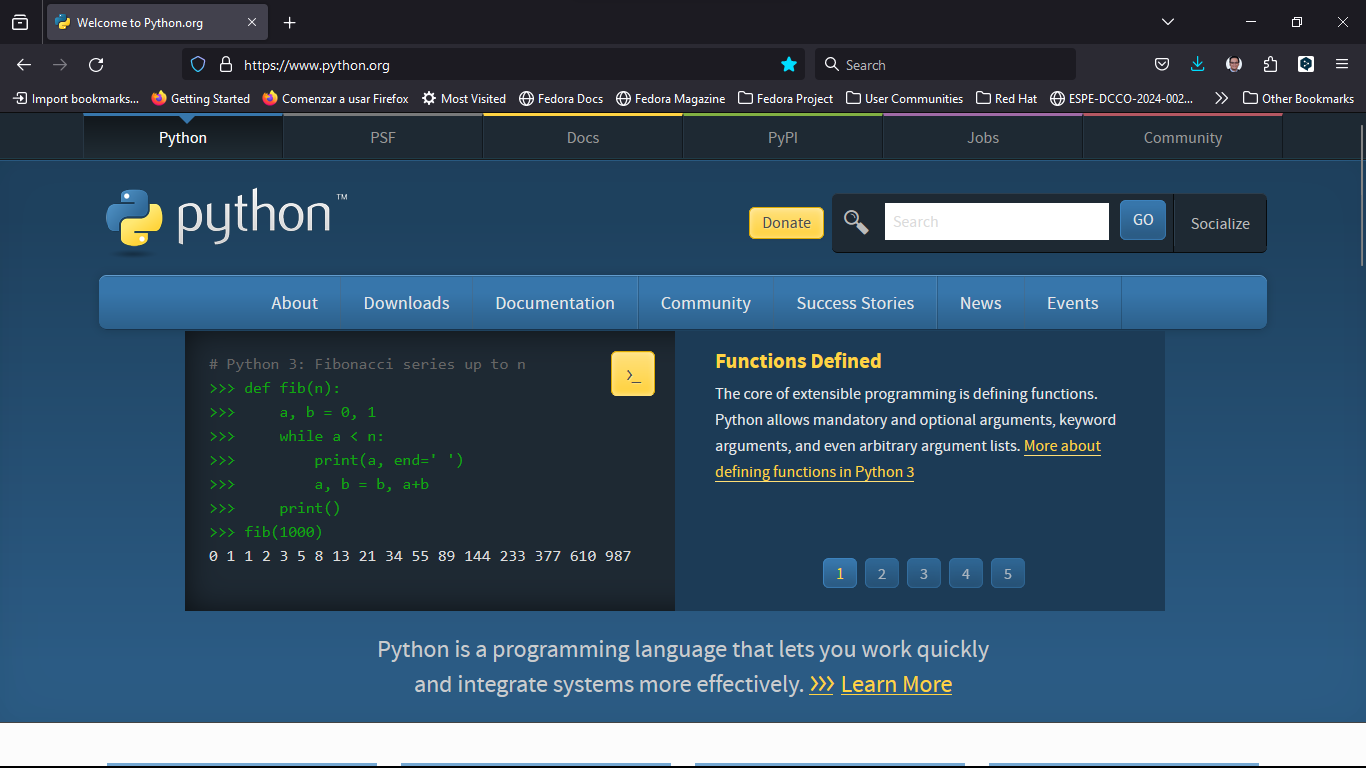
\includegraphics{unidades/unidad2/images/paste-1.png}

En la página de descargas, haga clic en el botón de descarga para la
última versión de Python. En el momento de escribir este tutorial, la
última versión de Python es 3.12.1

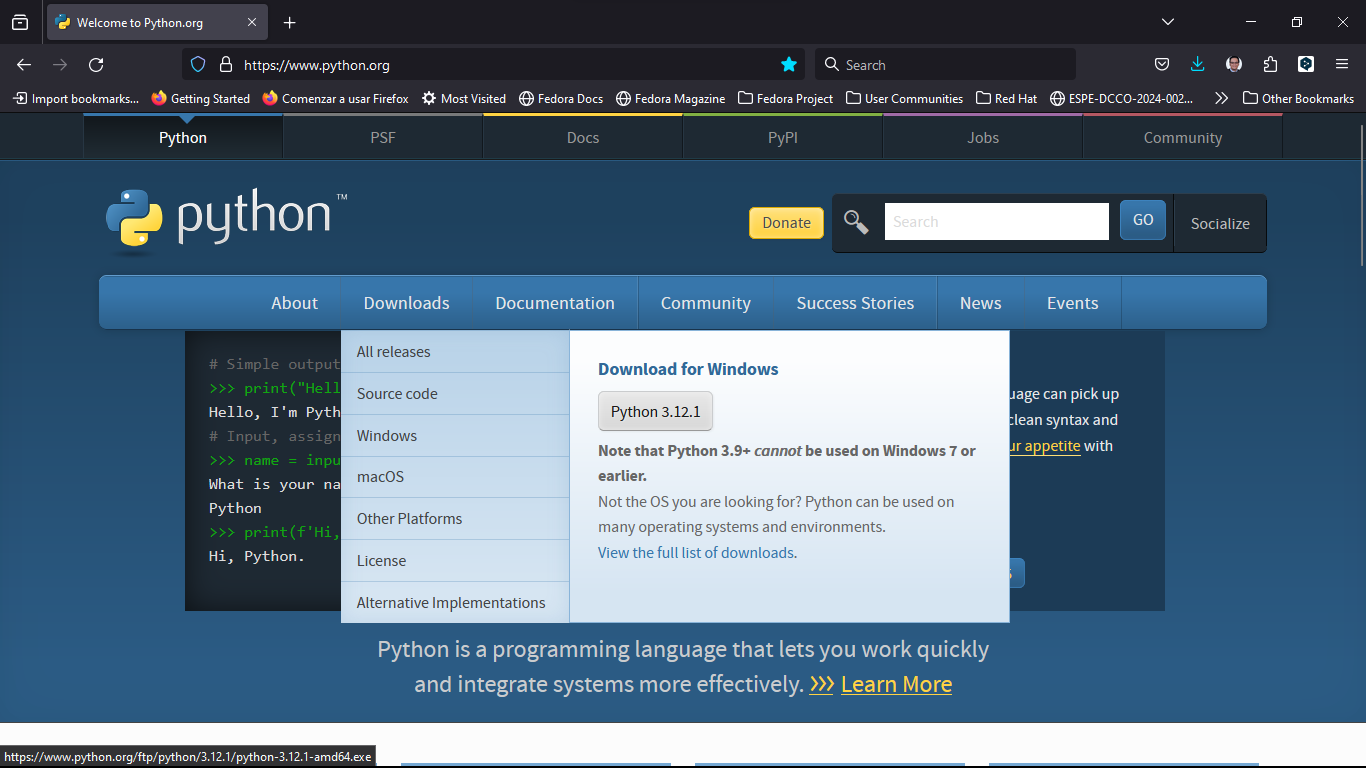
\includegraphics{unidades/unidad2/images/paste-2.png}

Excelente, ahora que hemos descargado el instalador de Python, podemos
continuar con la instalación de Python en Windows.

\begin{enumerate}
\def\labelenumi{\arabic{enumi}.}
\setcounter{enumi}{1}
\tightlist
\item
  \textbf{Instalar Python}
\end{enumerate}

Una vez que el instalador de Python se haya descargado, haga doble clic
en el archivo de instalación para iniciar el proceso de instalación.
Asegúrese de marcar la casilla que dice ``Add Python 3.12 to PATH''
antes de hacer clic en el botón ``Install Now''.


\includegraphics{unidades/unidad2/images/paste-4.png}

Ahora que hemos instalado Python en nuestra computadora, podemos
continuar con la configuración de nuestro entorno de desarrollo para
escribir y ejecutar programas en Python.

\begin{enumerate}
\def\labelenumi{\arabic{enumi}.}
\setcounter{enumi}{2}
\tightlist
\item
  \textbf{Comprobar que tenemos instalado Python}
\end{enumerate}

Para comprobar que Python se ha instalado correctamente en nuestra
computadora, abra una ventana de comandos y escriba el siguiente
comando:

\begin{Shaded}
\begin{Highlighting}[]
\ExtensionTok{python} \AttributeTok{{-}{-}version}
\end{Highlighting}
\end{Shaded}

\begin{enumerate}
\def\labelenumi{\arabic{enumi}.}
\setcounter{enumi}{3}
\tightlist
\item
  \textbf{Impresion de la versión de Python}
\end{enumerate}

Este comando imprimirá la versión de Python que está instalada en su
computadora. En mi caso, la versión de Python es 3.12.1.

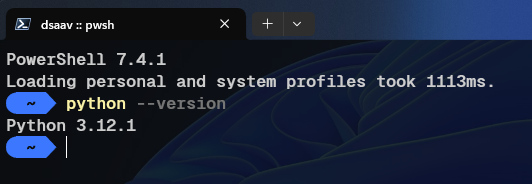
\includegraphics{unidades/unidad2/images/paste-5.png}

\subsection{Paso 3: Crear nuestro primer ``Hola Mundo'' en Python
🗺️.}\label{paso-3-crear-nuestro-primer-hola-mundo-en-python-.}

Ahora que hemos instalado Python en nuestra computadora, podemos
comenzar a escribir y ejecutar programas en Python. Para hacer esto,
necesitamos un editor de texto para escribir nuestro código y un
intérprete de Python para ejecutar nuestro código.

En este tutorial, usaremos Visual Studio Code como nuestro editor de
texto y el intérprete de Python que instalamos en el paso anterior.

\begin{enumerate}
\def\labelenumi{\arabic{enumi}.}
\tightlist
\item
  \textbf{Instalar Visual Studio Code}
\end{enumerate}

Para instalar Visual Studio Code, vaya al sitio web oficial de Visual
Studio Code en el siguiente enlace:

\url{https://code.visualstudio.com/}

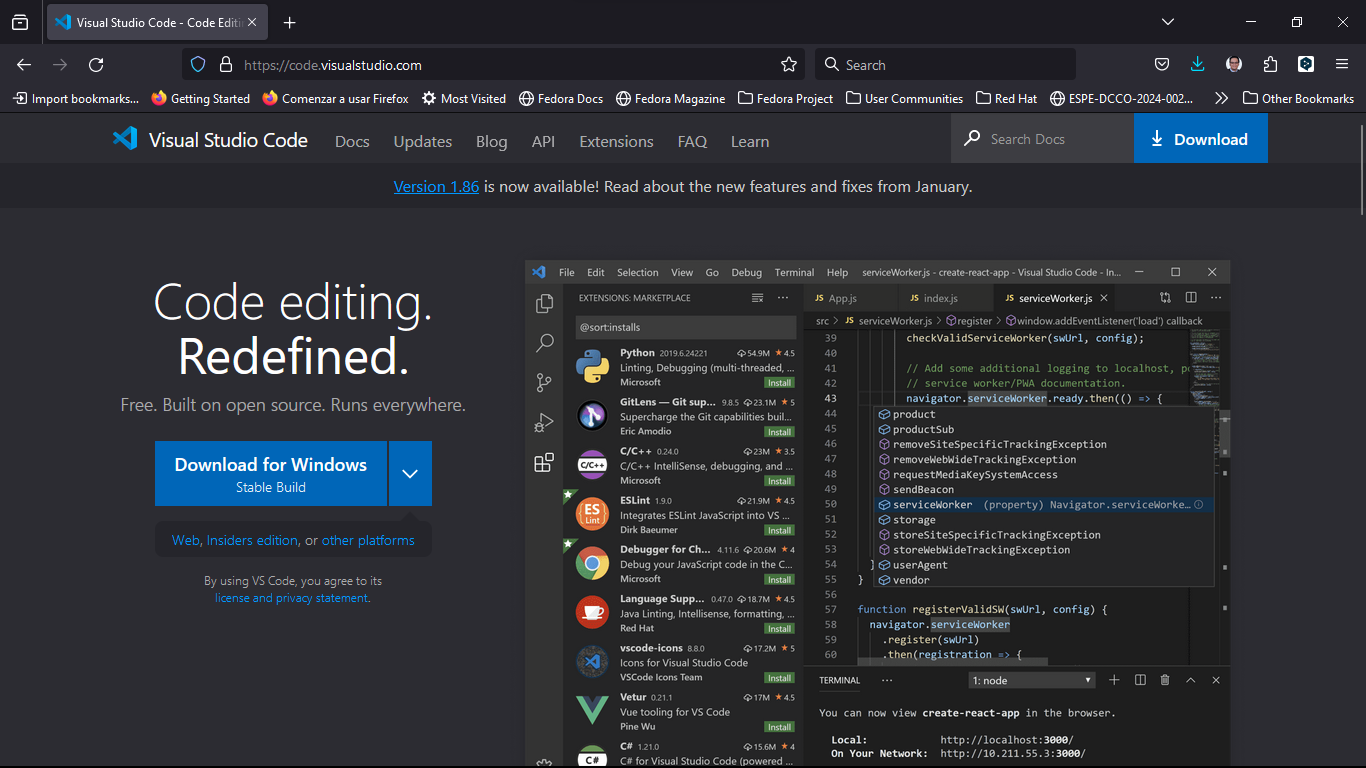
\includegraphics{unidades/unidad2/images/paste-6.png}

En la página de descargas, haga clic en el botón de descarga para su
sistema operativo. En el momento de escribir este tutorial, la última
versión de Visual Studio Code es 1.85.2.

Una vez que el instalador de Visual Studio Code se haya descargado, haga
doble clic en el archivo de instalación para iniciar el proceso de
instalación. Siga las instrucciones en pantalla para completar la
instalación.

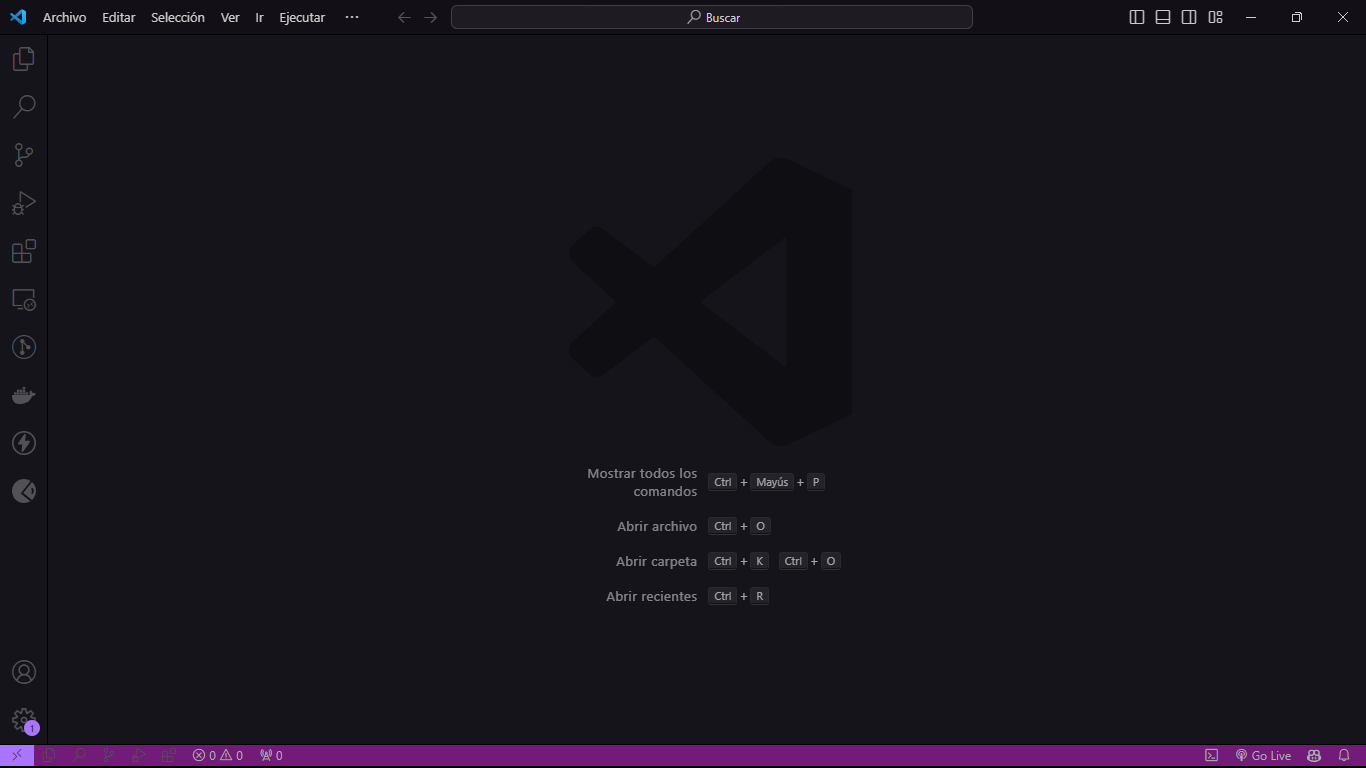
\includegraphics{unidades/unidad2/images/paste-7.png}

\begin{enumerate}
\def\labelenumi{\arabic{enumi}.}
\setcounter{enumi}{1}
\tightlist
\item
  \textbf{Crear un nuevo archivo de Python}
\end{enumerate}

Para crear un nuevo archivo de Python en Visual Studio Code, abra Visual
Studio Code y haga clic en el botón ``New File'' en la barra de
herramientas. Luego, escriba el siguiente código en el archivo:

\begin{Shaded}
\begin{Highlighting}[]
\BuiltInTok{print}\NormalTok{(}\StringTok{"Hola Mundo"}\NormalTok{)}
\end{Highlighting}
\end{Shaded}

\begin{enumerate}
\def\labelenumi{\arabic{enumi}.}
\setcounter{enumi}{2}
\tightlist
\item
  Este código imprimirá ``Hola Mundo'' en la consola.
\end{enumerate}

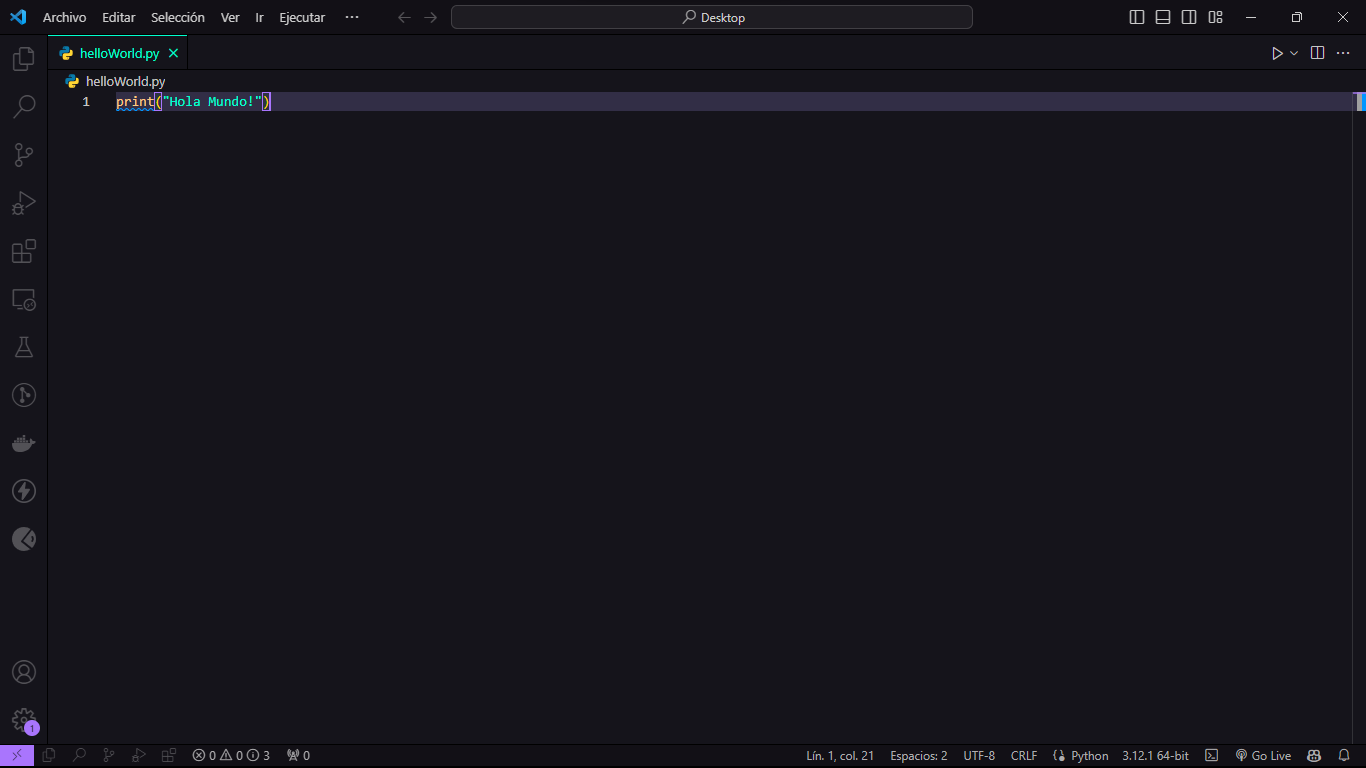
\includegraphics{unidades/unidad2/images/paste-8.png}

\begin{enumerate}
\def\labelenumi{\arabic{enumi}.}
\setcounter{enumi}{3}
\tightlist
\item
  Ejecutar el programa
\end{enumerate}

Para ejecutar el programa, haga clic en el botón ``Run'' en la barra de
herramientas. Esto ejecutará el programa y mostrará ``Hola Mundo'' en la
consola.

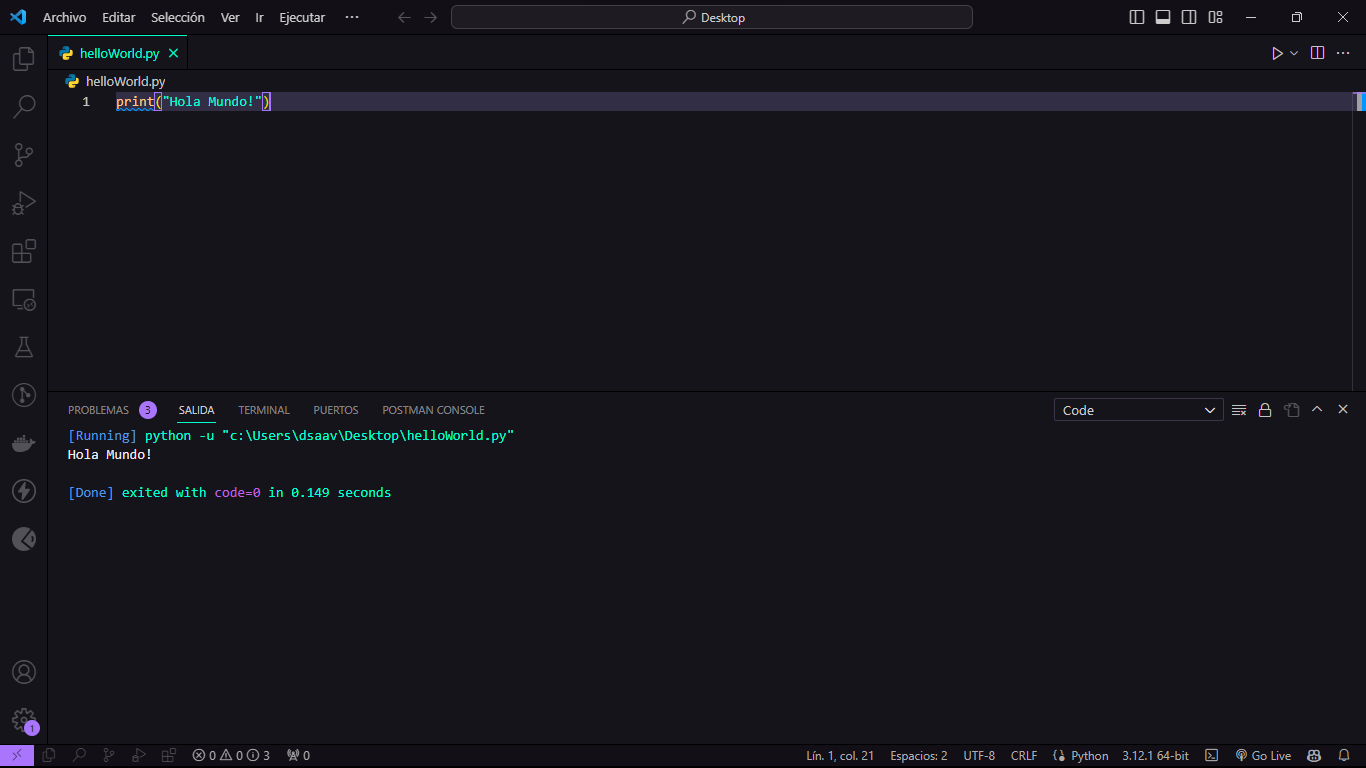
\includegraphics{unidades/unidad2/images/paste-9.png}

¡Felicidades!

Acabas de escribir y ejecutar tu primer programa en Python. Ahora que
has configurado tu entorno de desarrollo y has escrito tu primer
programa en Python, puedes comenzar a explorar el lenguaje de
programación Python y aprender a escribir programas más complejos.

\chapter{Sintaxis Básica}\label{sintaxis-buxe1sica}

\begin{figure}[H]

{\centering 
\includegraphics[width=2.08333in,height=\textheight]{unidades/unidad2/../../images/python-logo.png}

}

\caption{Python}

\end{figure}%

\phantomsection\label{annotated-cell-25}%
\begin{Shaded}
\begin{Highlighting}[]
\ControlFlowTok{if} \DecValTok{5} \OperatorTok{\textgreater{}} \DecValTok{2}\NormalTok{:}
  \BuiltInTok{print}\NormalTok{(}\StringTok{"Cinco es mayor que dos"}\NormalTok{) }\hspace*{\fill}\NormalTok{\circled{1}}
\end{Highlighting}
\end{Shaded}

\begin{description}
\tightlist
\item[\circled{1}]
En el ejemplo anterior, la instrucción \textbf{print} está indentada, es
decir, tiene un espacio al principio de la línea. Esto es necesario para
que el código funcione correctamente.
\end{description}

Además de la indentación, en python se utilizan los dos puntos
\textbf{:} para indicar que se va a escribir un bloque de código.

\phantomsection\label{annotated-cell-26}%
\begin{Shaded}
\begin{Highlighting}[]
\ControlFlowTok{if} \DecValTok{5} \OperatorTok{\textgreater{}} \DecValTok{2}\NormalTok{: }\hspace*{\fill}\NormalTok{\circled{1}}
  \BuiltInTok{print}\NormalTok{(}\StringTok{"Cinco es mayor que dos"}\NormalTok{) }
\end{Highlighting}
\end{Shaded}

\begin{description}
\tightlist
\item[\circled{1}]
En este caso, el \textbf{:} indica que se va a escribir un bloque de
código, el bloque de código que se ejecutará si la condición es
verdadera.
\end{description}

\chapter{Comentarios}\label{comentarios}

Los comentarios en python se escriben con el símbolo \textbf{\#}.

\phantomsection\label{annotated-cell-27}%
\begin{Shaded}
\begin{Highlighting}[]
\CommentTok{\# Este es un comentario}
\BuiltInTok{print}\NormalTok{(}\StringTok{"Hola Mundo"}\NormalTok{) }\hspace*{\fill}\NormalTok{\circled{1}}
\end{Highlighting}
\end{Shaded}

\begin{description}
\tightlist
\item[\circled{1}]
En este caso, el comentario está al final de la línea de código.
\end{description}

\chapter{Variables y Tipos de Datos}\label{variables-y-tipos-de-datos}

\begin{tcolorbox}[enhanced jigsaw, breakable, titlerule=0mm, colframe=quarto-callout-tip-color-frame, left=2mm, opacityback=0, rightrule=.15mm, colback=white, opacitybacktitle=0.6, title=\textcolor{quarto-callout-tip-color}{\faLightbulb}\hspace{0.5em}{Tip}, toprule=.15mm, bottomtitle=1mm, leftrule=.75mm, colbacktitle=quarto-callout-tip-color!10!white, toptitle=1mm, coltitle=black, arc=.35mm, bottomrule=.15mm]

Existe la forma de declarar variables de python con su tipo de dato

Ejemplo:

\phantomsection\label{annotated-cell-185}%
\begin{Shaded}
\begin{Highlighting}[]
\NormalTok{x: }\BuiltInTok{int} \OperatorTok{=} \DecValTok{5} \hspace*{\fill}\NormalTok{\circled{1}}
\NormalTok{y: }\BuiltInTok{str} \OperatorTok{=} \StringTok{"Hola Mundo"} \hspace*{\fill}\NormalTok{\circled{2}}
\end{Highlighting}
\end{Shaded}

\begin{description}
\tightlist
\item[\circled{1}]
En este caso, la variable \textbf{x} es de tipo entero.
\item[\circled{2}]
En este caso, la variable \textbf{y} es de tipo cadena de texto.
\end{description}

\end{tcolorbox}

En python, las variables se definen de la siguiente manera:

\phantomsection\label{annotated-cell-28}%
\begin{Shaded}
\begin{Highlighting}[]
\NormalTok{x }\OperatorTok{=} \DecValTok{5} \hspace*{\fill}\NormalTok{\circled{1}}
\NormalTok{y }\OperatorTok{=} \StringTok{"Hola Mundo"} \hspace*{\fill}\NormalTok{\circled{2}}
\end{Highlighting}
\end{Shaded}

\begin{description}
\tightlist
\item[\circled{1}]
En este caso, la variable \textbf{x} es de tipo entero.
\item[\circled{2}]
En este caso, la variable \textbf{y} es de tipo cadena de texto.
\end{description}

\chapter{Tipos de Datos}\label{tipos-de-datos}

En python, los tipos de datos más comunes son:

\begin{itemize}
\tightlist
\item
  \textbf{int}: Entero
\end{itemize}

Ejemplo:

\phantomsection\label{annotated-cell-29}%
\begin{Shaded}
\begin{Highlighting}[]
\NormalTok{x }\OperatorTok{=} \DecValTok{5} \hspace*{\fill}\NormalTok{\circled{1}}
\end{Highlighting}
\end{Shaded}

\begin{description}
\tightlist
\item[\circled{1}]
La variable \textbf{x} es de tipo entero.
\end{description}

\begin{itemize}
\tightlist
\item
  \textbf{float}: Flotante
\end{itemize}

Ejemplo:

\phantomsection\label{annotated-cell-30}%
\begin{Shaded}
\begin{Highlighting}[]
\NormalTok{y }\OperatorTok{=} \FloatTok{5.0} \hspace*{\fill}\NormalTok{\circled{1}}
\end{Highlighting}
\end{Shaded}

\begin{description}
\tightlist
\item[\circled{1}]
La variable \textbf{y} es de tipo flotante.
\end{description}

\begin{itemize}
\tightlist
\item
  \textbf{str}: Cadena de texto
\end{itemize}

Ejemplo:

\phantomsection\label{annotated-cell-31}%
\begin{Shaded}
\begin{Highlighting}[]
\NormalTok{z }\OperatorTok{=} \StringTok{"Hola Mundo"} \hspace*{\fill}\NormalTok{\circled{1}}
\end{Highlighting}
\end{Shaded}

\begin{itemize}
\tightlist
\item
  \textbf{bool}: Booleano
\end{itemize}

Ejemplo:

\phantomsection\label{annotated-cell-32}%
\begin{Shaded}
\begin{Highlighting}[]
\NormalTok{a }\OperatorTok{=} \VariableTok{True} \hspace*{\fill}\NormalTok{\circled{1}}
\end{Highlighting}
\end{Shaded}

\begin{description}
\tightlist
\item[\circled{1}]
La variable \textbf{a} es de tipo booleano.
\end{description}

\begin{itemize}
\tightlist
\item
  \textbf{list}: Lista
\end{itemize}

Ejemplo:

\phantomsection\label{annotated-cell-33}%
\begin{Shaded}
\begin{Highlighting}[]
\NormalTok{b }\OperatorTok{=}\NormalTok{ [}\DecValTok{1}\NormalTok{, }\DecValTok{2}\NormalTok{, }\DecValTok{3}\NormalTok{] }\hspace*{\fill}\NormalTok{\circled{1}}
\end{Highlighting}
\end{Shaded}

\begin{itemize}
\tightlist
\item
  \textbf{tuple}: Tupla
\end{itemize}

Ejemplo:

\phantomsection\label{annotated-cell-34}%
\begin{Shaded}
\begin{Highlighting}[]
\NormalTok{c }\OperatorTok{=}\NormalTok{ (}\DecValTok{1}\NormalTok{, }\DecValTok{2}\NormalTok{, }\DecValTok{3}\NormalTok{) }\hspace*{\fill}\NormalTok{\circled{1}}
\end{Highlighting}
\end{Shaded}

\begin{itemize}
\tightlist
\item
  \textbf{dict}: Diccionario
\end{itemize}

Ejemplo:

\phantomsection\label{annotated-cell-35}%
\begin{Shaded}
\begin{Highlighting}[]
\NormalTok{d }\OperatorTok{=}\NormalTok{ \{}\StringTok{"nombre"}\NormalTok{: }\StringTok{"Juan"}\NormalTok{, }\StringTok{"edad"}\NormalTok{: }\DecValTok{25}\NormalTok{\} }\hspace*{\fill}\NormalTok{\circled{1}}
\end{Highlighting}
\end{Shaded}

\begin{itemize}
\tightlist
\item
  \textbf{set}: Conjunto
\end{itemize}

Ejemplo:

\phantomsection\label{annotated-cell-36}%
\begin{Shaded}
\begin{Highlighting}[]
\NormalTok{e }\OperatorTok{=}\NormalTok{ \{}\DecValTok{1}\NormalTok{, }\DecValTok{2}\NormalTok{, }\DecValTok{3}\NormalTok{\} }\hspace*{\fill}\NormalTok{\circled{1}}
\end{Highlighting}
\end{Shaded}

\begin{description}
\tightlist
\item[\circled{1}]
La variable \textbf{e} es de tipo conjunto.
\end{description}

\begin{itemize}
\tightlist
\item
  \textbf{None}: Nulo
\end{itemize}

Ejemplo:

\phantomsection\label{annotated-cell-37}%
\begin{Shaded}
\begin{Highlighting}[]
\NormalTok{f }\OperatorTok{=} \VariableTok{None} \hspace*{\fill}\NormalTok{\circled{1}}
\end{Highlighting}
\end{Shaded}

\begin{description}
\tightlist
\item[\circled{1}]
La variable \textbf{f} es de tipo \textbf{None}.
\end{description}

\chapter{Operadores}\label{operadores}

En python, los operadores más comunes son:

\begin{itemize}
\tightlist
\item
  \textbf{+}: Suma
\end{itemize}

Ejemplo:

\phantomsection\label{annotated-cell-38}%
\begin{Shaded}
\begin{Highlighting}[]
\NormalTok{x }\OperatorTok{=} \DecValTok{5}
\NormalTok{y }\OperatorTok{=} \DecValTok{2}
\NormalTok{z }\OperatorTok{=}\NormalTok{ x }\OperatorTok{+}\NormalTok{ y }\hspace*{\fill}\NormalTok{\circled{1}}
\end{Highlighting}
\end{Shaded}

\begin{description}
\tightlist
\item[\circled{1}]
La variable \textbf{z} es igual a la suma de \textbf{x} y \textbf{y}.
\end{description}

\begin{itemize}
\tightlist
\item
  \textbf{-}: Resta
\end{itemize}

Ejemplo:

\phantomsection\label{annotated-cell-39}%
\begin{Shaded}
\begin{Highlighting}[]
\NormalTok{x }\OperatorTok{=} \DecValTok{5}
\NormalTok{y }\OperatorTok{=} \DecValTok{2}
\NormalTok{a }\OperatorTok{=}\NormalTok{ x }\OperatorTok{{-}}\NormalTok{ y }\hspace*{\fill}\NormalTok{\circled{1}}
\end{Highlighting}
\end{Shaded}

\begin{description}
\tightlist
\item[\circled{1}]
La variable \textbf{a} es igual a la resta de \textbf{x} y \textbf{y}.
\end{description}

\begin{itemize}
\tightlist
\item
  **``*``**: Multiplicación
\end{itemize}

Ejemplo:

\phantomsection\label{annotated-cell-40}%
\begin{Shaded}
\begin{Highlighting}[]
\NormalTok{x }\OperatorTok{=} \DecValTok{5}
\NormalTok{y }\OperatorTok{=} \DecValTok{2}
\NormalTok{b }\OperatorTok{=}\NormalTok{ x }\OperatorTok{*}\NormalTok{ y }\hspace*{\fill}\NormalTok{\circled{1}}
\end{Highlighting}
\end{Shaded}

\begin{description}
\tightlist
\item[\circled{1}]
La variable \textbf{b} es igual a la multiplicación de \textbf{x} y
\textbf{y}.
\end{description}

\begin{itemize}
\tightlist
\item
  \textbf{/}: División
\end{itemize}

Ejemplo:

\phantomsection\label{annotated-cell-41}%
\begin{Shaded}
\begin{Highlighting}[]
\NormalTok{x }\OperatorTok{=} \DecValTok{5}
\NormalTok{y }\OperatorTok{=} \DecValTok{2}
\NormalTok{c }\OperatorTok{=}\NormalTok{ x }\OperatorTok{/}\NormalTok{ y }\hspace*{\fill}\NormalTok{\circled{1}}
\end{Highlighting}
\end{Shaded}

\begin{description}
\tightlist
\item[\circled{1}]
La variable \textbf{c} es igual a la división de \textbf{x} y
\textbf{y}.
\end{description}

\begin{itemize}
\tightlist
\item
  \textbf{//}: División entera
\end{itemize}

Ejemplo:

\phantomsection\label{annotated-cell-42}%
\begin{Shaded}
\begin{Highlighting}[]
\NormalTok{x }\OperatorTok{=} \DecValTok{5}
\NormalTok{y }\OperatorTok{=} \DecValTok{2}
\NormalTok{d }\OperatorTok{=}\NormalTok{ x }\OperatorTok{//}\NormalTok{ y }\hspace*{\fill}\NormalTok{\circled{1}}
\end{Highlighting}
\end{Shaded}

\begin{description}
\tightlist
\item[\circled{1}]
La variable \textbf{d} es igual a la división entera de \textbf{x} y
\textbf{y}.
\end{description}

\begin{itemize}
\tightlist
\item
  \textbf{\%}: Módulo
\end{itemize}

Ejemplo:

\phantomsection\label{annotated-cell-43}%
\begin{Shaded}
\begin{Highlighting}[]
\NormalTok{x }\OperatorTok{=} \DecValTok{5}
\NormalTok{y }\OperatorTok{=} \DecValTok{2}
\NormalTok{e }\OperatorTok{=}\NormalTok{ x }\OperatorTok{\%}\NormalTok{ y }\hspace*{\fill}\NormalTok{\circled{1}}
\end{Highlighting}
\end{Shaded}

\begin{description}
\tightlist
\item[\circled{1}]
La variable \textbf{e} es igual al módulo de \textbf{x} y \textbf{y}.
\end{description}

\begin{itemize}
\tightlist
\item
  \textbf{``}''**: Potencia
\end{itemize}

Ejemplo:

\phantomsection\label{annotated-cell-44}%
\begin{Shaded}
\begin{Highlighting}[]
\NormalTok{x }\OperatorTok{=} \DecValTok{5}
\NormalTok{y }\OperatorTok{=} \DecValTok{2}
\NormalTok{f }\OperatorTok{=}\NormalTok{ x }\OperatorTok{**}\NormalTok{ y }\hspace*{\fill}\NormalTok{\circled{1}}
\end{Highlighting}
\end{Shaded}

\begin{description}
\tightlist
\item[\circled{1}]
La variable \textbf{f} es igual a la potencia de \textbf{x} y
\textbf{y}.
\end{description}

\begin{itemize}
\tightlist
\item
  \textbf{==}: Igualdad
\end{itemize}

Ejemplo:

\phantomsection\label{annotated-cell-45}%
\begin{Shaded}
\begin{Highlighting}[]
\NormalTok{x }\OperatorTok{=} \DecValTok{5}
\NormalTok{y }\OperatorTok{=} \DecValTok{2}
\NormalTok{g }\OperatorTok{=}\NormalTok{ x }\OperatorTok{==}\NormalTok{ y }\hspace*{\fill}\NormalTok{\circled{1}}
\end{Highlighting}
\end{Shaded}

\begin{description}
\tightlist
\item[\circled{1}]
La variable \textbf{g} es igual a la comparación de igualdad entre
\textbf{x} y \textbf{y}.
\end{description}

\begin{itemize}
\tightlist
\item
  \textbf{!=}: Diferente
\end{itemize}

Ejemplo:

\phantomsection\label{annotated-cell-46}%
\begin{Shaded}
\begin{Highlighting}[]
\NormalTok{x }\OperatorTok{=} \DecValTok{5}
\NormalTok{y }\OperatorTok{=} \DecValTok{2}
\NormalTok{h }\OperatorTok{=}\NormalTok{ x }\OperatorTok{!=}\NormalTok{ y }\hspace*{\fill}\NormalTok{\circled{1}}
\end{Highlighting}
\end{Shaded}

\begin{description}
\tightlist
\item[\circled{1}]
La variable \textbf{h} es igual a la comparación de diferencia entre
\textbf{x} y \textbf{y}.
\end{description}

\begin{itemize}
\tightlist
\item
  \textbf{\textgreater{}}: Mayor que
\end{itemize}

Ejemplo:

\phantomsection\label{annotated-cell-47}%
\begin{Shaded}
\begin{Highlighting}[]
\NormalTok{x }\OperatorTok{=} \DecValTok{5}
\NormalTok{y }\OperatorTok{=} \DecValTok{2}
\NormalTok{i }\OperatorTok{=}\NormalTok{ x }\OperatorTok{\textgreater{}}\NormalTok{ y }\hspace*{\fill}\NormalTok{\circled{1}}
\end{Highlighting}
\end{Shaded}

\begin{itemize}
\tightlist
\item
  \textbf{\textless{}}: Menor que
\end{itemize}

Ejemplo:

\phantomsection\label{annotated-cell-48}%
\begin{Shaded}
\begin{Highlighting}[]
\NormalTok{x }\OperatorTok{=} \DecValTok{5}
\NormalTok{y }\OperatorTok{=} \DecValTok{2}
\NormalTok{j }\OperatorTok{=}\NormalTok{ x }\OperatorTok{\textless{}}\NormalTok{ y }\hspace*{\fill}\NormalTok{\circled{1}}
\end{Highlighting}
\end{Shaded}

\begin{description}
\tightlist
\item[\circled{1}]
La variable \textbf{j} es igual a la comparación de menor que entre
\textbf{x} y \textbf{y}.
\end{description}

\begin{itemize}
\tightlist
\item
  \textbf{\textgreater=}: Mayor
\end{itemize}

Ejemplo:

\phantomsection\label{annotated-cell-49}%
\begin{Shaded}
\begin{Highlighting}[]
\NormalTok{x }\OperatorTok{=} \DecValTok{5}
\NormalTok{y }\OperatorTok{=} \DecValTok{2}
\NormalTok{k }\OperatorTok{=}\NormalTok{ x }\OperatorTok{\textgreater{}=}\NormalTok{ y }\hspace*{\fill}\NormalTok{\circled{1}}
\end{Highlighting}
\end{Shaded}

\begin{description}
\tightlist
\item[\circled{1}]
La variable \textbf{k} es igual a la comparación de mayor o igual que
entre \textbf{x} y \textbf{y}.
\end{description}

\begin{itemize}
\tightlist
\item
  \textbf{\textless=}: Menor
\end{itemize}

Ejemplo:

\phantomsection\label{annotated-cell-50}%
\begin{Shaded}
\begin{Highlighting}[]
\NormalTok{x }\OperatorTok{=} \DecValTok{5}
\NormalTok{y }\OperatorTok{=} \DecValTok{2}
\NormalTok{l }\OperatorTok{=}\NormalTok{ x }\OperatorTok{\textless{}=}\NormalTok{ y }\hspace*{\fill}\NormalTok{\circled{1}}
\end{Highlighting}
\end{Shaded}

\begin{description}
\tightlist
\item[\circled{1}]
La variable \textbf{l} es igual a la comparación de menor o igual que
entre \textbf{x} y \textbf{y}.
\end{description}

\begin{itemize}
\tightlist
\item
  \textbf{and}: Y
\end{itemize}

Ejemplo:

\phantomsection\label{annotated-cell-51}%
\begin{Shaded}
\begin{Highlighting}[]
\NormalTok{x }\OperatorTok{=} \DecValTok{5}
\NormalTok{y }\OperatorTok{=} \DecValTok{2}
\NormalTok{m }\OperatorTok{=}\NormalTok{ x }\KeywordTok{and}\NormalTok{ y }\hspace*{\fill}\NormalTok{\circled{1}}
\end{Highlighting}
\end{Shaded}

\begin{itemize}
\tightlist
\item
  \textbf{or}: O
\end{itemize}

Ejemplo:

\phantomsection\label{annotated-cell-52}%
\begin{Shaded}
\begin{Highlighting}[]
\NormalTok{x }\OperatorTok{=} \DecValTok{5}
\NormalTok{y }\OperatorTok{=} \DecValTok{2}
\NormalTok{n }\OperatorTok{=}\NormalTok{ x }\KeywordTok{or}\NormalTok{ y }\hspace*{\fill}\NormalTok{\circled{1}}
\end{Highlighting}
\end{Shaded}

\begin{description}
\tightlist
\item[\circled{1}]
La variable \textbf{n} es igual a la comparación lógica \textbf{or}
entre \textbf{x} y \textbf{y}.
\end{description}

\begin{itemize}
\tightlist
\item
  \textbf{not}: Negación
\end{itemize}

Ejemplo:

\phantomsection\label{annotated-cell-53}%
\begin{Shaded}
\begin{Highlighting}[]
\NormalTok{x }\OperatorTok{=} \DecValTok{5}
\NormalTok{o }\OperatorTok{=} \KeywordTok{not}\NormalTok{ x }\hspace*{\fill}\NormalTok{\circled{1}}
\end{Highlighting}
\end{Shaded}

\begin{description}
\tightlist
\item[\circled{1}]
La variable \textbf{o} es igual a la negación de \textbf{x}.
\end{description}

\chapter{Estructura de Control}\label{estructura-de-control}

En python, las estructuras de control más comunes son:

\begin{itemize}
\tightlist
\item
  \textbf{if}: Si
\end{itemize}

Ejemplo:

\phantomsection\label{annotated-cell-54}%
\begin{Shaded}
\begin{Highlighting}[]
\ControlFlowTok{if} \DecValTok{5} \OperatorTok{\textgreater{}} \DecValTok{2}\NormalTok{: }\hspace*{\fill}\NormalTok{\circled{1}}
  \BuiltInTok{print}\NormalTok{(}\StringTok{"Cinco es mayor que dos"}\NormalTok{) }\hspace*{\fill}\NormalTok{\circled{2}}
\end{Highlighting}
\end{Shaded}

\begin{description}
\tightlist
\item[\circled{1}]
En este caso, se evalúa si 5 es mayor que 2.
\item[\circled{2}]
Si la condición es verdadera, se imprime el mensaje ``Cinco es mayor que
dos''.
\end{description}

\begin{itemize}
\tightlist
\item
  \textbf{elif}: Si no
\end{itemize}

Ejemplo:

\phantomsection\label{annotated-cell-55}%
\begin{Shaded}
\begin{Highlighting}[]
\NormalTok{x }\OperatorTok{=} \DecValTok{5}
\NormalTok{y }\OperatorTok{=} \DecValTok{2}
\ControlFlowTok{if}\NormalTok{ x }\OperatorTok{\textgreater{}}\NormalTok{ y: }\hspace*{\fill}\NormalTok{\circled{1}}
  \BuiltInTok{print}\NormalTok{(}\StringTok{"X es mayor que Y"}\NormalTok{) }\hspace*{\fill}\NormalTok{\circled{2}}
\ControlFlowTok{elif}\NormalTok{ x }\OperatorTok{\textless{}}\NormalTok{ y: }\hspace*{\fill}\NormalTok{\circled{3}}
  \BuiltInTok{print}\NormalTok{(}\StringTok{"X es menor que Y"}\NormalTok{) }\hspace*{\fill}\NormalTok{\circled{4}}
\end{Highlighting}
\end{Shaded}

\begin{description}
\tightlist
\item[\circled{1}]
En este caso, se evalúa si \textbf{x} es mayor que \textbf{y}.
\item[\circled{2}]
Si la condición es verdadera, se imprime el mensaje ``X es mayor que
Y''.
\item[\circled{3}]
Si la condición anterior es falsa, se evalúa si \textbf{x} es menor que
\textbf{y}.
\item[\circled{4}]
Si la condición es verdadera, se imprime el mensaje ``X es menor que
Y''.
\end{description}

\begin{itemize}
\tightlist
\item
  \textbf{else}: Si no
\end{itemize}

Ejemplo:

\phantomsection\label{annotated-cell-56}%
\begin{Shaded}
\begin{Highlighting}[]
\NormalTok{x }\OperatorTok{=} \DecValTok{5}
\NormalTok{y }\OperatorTok{=} \DecValTok{2}
\ControlFlowTok{if}\NormalTok{ x }\OperatorTok{\textgreater{}}\NormalTok{ y: }\hspace*{\fill}\NormalTok{\circled{1}}
  \BuiltInTok{print}\NormalTok{(}\StringTok{"X es mayor que Y"}\NormalTok{) }\hspace*{\fill}\NormalTok{\circled{2}}
\ControlFlowTok{elif}\NormalTok{ x }\OperatorTok{\textless{}}\NormalTok{ y: }\hspace*{\fill}\NormalTok{\circled{3}}
  \BuiltInTok{print}\NormalTok{(}\StringTok{"X es menor que Y"}\NormalTok{) }\hspace*{\fill}\NormalTok{\circled{4}}
\ControlFlowTok{else}\NormalTok{: }\hspace*{\fill}\NormalTok{\circled{5}}
  \BuiltInTok{print}\NormalTok{(}\StringTok{"X es igual a Y"}\NormalTok{) }\hspace*{\fill}\NormalTok{\circled{6}}
\end{Highlighting}
\end{Shaded}

\begin{description}
\tightlist
\item[\circled{1}]
En este caso, se evalúa si \textbf{x} es mayor que \textbf{y}.
\item[\circled{2}]
Si la condición es verdadera, se imprime el mensaje ``X es mayor que
Y''.
\item[\circled{3}]
Si la condición anterior es falsa, se evalúa si \textbf{x} es menor que
\textbf{y}.
\item[\circled{4}]
Si la condición es verdadera, se imprime el mensaje ``X es menor que
Y''.
\item[\circled{5}]
Si las condiciones anteriores son falsas, se ejecuta el bloque de código
del \textbf{else}.
\item[\circled{6}]
En este caso, se imprime el mensaje ``X es igual a Y''.
\end{description}

\begin{itemize}
\tightlist
\item
  \textbf{for}: Para
\end{itemize}

Ejemplo:

\phantomsection\label{annotated-cell-57}%
\begin{Shaded}
\begin{Highlighting}[]
\ControlFlowTok{for}\NormalTok{ x }\KeywordTok{in} \BuiltInTok{range}\NormalTok{(}\DecValTok{5}\NormalTok{): }\hspace*{\fill}\NormalTok{\circled{1}}
  \BuiltInTok{print}\NormalTok{(x) }\hspace*{\fill}\NormalTok{\circled{2}}
\end{Highlighting}
\end{Shaded}

\begin{description}
\tightlist
\item[\circled{1}]
En este caso, se recorre un rango de 0 a 5.
\item[\circled{2}]
En cada iteración, se imprime el valor de \textbf{x}.
\end{description}

\begin{itemize}
\tightlist
\item
  \textbf{while}: Mientras
\end{itemize}

Ejemplo:

\phantomsection\label{annotated-cell-58}%
\begin{Shaded}
\begin{Highlighting}[]
\NormalTok{x }\OperatorTok{=} \DecValTok{0}
\ControlFlowTok{while}\NormalTok{ x }\OperatorTok{\textless{}} \DecValTok{5}\NormalTok{: }\hspace*{\fill}\NormalTok{\circled{1}}
  \BuiltInTok{print}\NormalTok{(x) }\hspace*{\fill}\NormalTok{\circled{2}}
\NormalTok{  x }\OperatorTok{+=} \DecValTok{1} \hspace*{\fill}\NormalTok{\circled{3}}
\end{Highlighting}
\end{Shaded}

\begin{description}
\tightlist
\item[\circled{1}]
En este caso, se evalúa si \textbf{x} es menor que 5.
\item[\circled{2}]
En cada iteración, se imprime el valor de \textbf{x}.
\item[\circled{3}]
En cada iteración, se incrementa el valor de \textbf{x}.
\end{description}

\begin{itemize}
\tightlist
\item
  \textbf{break}: Romper
\end{itemize}

Ejemplo:

\phantomsection\label{annotated-cell-59}%
\begin{Shaded}
\begin{Highlighting}[]
\NormalTok{x }\OperatorTok{=} \DecValTok{0}
\ControlFlowTok{while}\NormalTok{ x }\OperatorTok{\textless{}} \DecValTok{5}\NormalTok{: }\hspace*{\fill}\NormalTok{\circled{1}}
  \BuiltInTok{print}\NormalTok{(x) }\hspace*{\fill}\NormalTok{\circled{2}}
\NormalTok{  x }\OperatorTok{+=} \DecValTok{1} \hspace*{\fill}\NormalTok{\circled{3}}
  \ControlFlowTok{if}\NormalTok{ x }\OperatorTok{==} \DecValTok{3}\NormalTok{: }\hspace*{\fill}\NormalTok{\circled{4}}
    \ControlFlowTok{break} \hspace*{\fill}\NormalTok{\circled{5}}
\end{Highlighting}
\end{Shaded}

\begin{description}
\tightlist
\item[\circled{1}]
En este caso, se evalúa si \textbf{x} es menor que 5.
\item[\circled{2}]
En cada iteración, se imprime el valor de \textbf{x}.
\item[\circled{3}]
En cada iteración, se incrementa el valor de \textbf{x}.
\item[\circled{4}]
En cada iteración, se evalúa si \textbf{x} es igual a 3.
\item[\circled{5}]
Si la condición es verdadera, se rompe el ciclo.
\end{description}

\begin{itemize}
\tightlist
\item
  \textbf{continue}: Continuar
\end{itemize}

Ejemplo:

\phantomsection\label{annotated-cell-60}%
\begin{Shaded}
\begin{Highlighting}[]
\NormalTok{x }\OperatorTok{=} \DecValTok{0}
\ControlFlowTok{while}\NormalTok{ x }\OperatorTok{\textless{}} \DecValTok{5}\NormalTok{: }\hspace*{\fill}\NormalTok{\circled{1}}
\NormalTok{  x }\OperatorTok{+=} \DecValTok{1} \hspace*{\fill}\NormalTok{\circled{2}}
  \ControlFlowTok{if}\NormalTok{ x }\OperatorTok{==} \DecValTok{3}\NormalTok{: }\hspace*{\fill}\NormalTok{\circled{3}}
    \ControlFlowTok{continue} \hspace*{\fill}\NormalTok{\circled{4}}
  \BuiltInTok{print}\NormalTok{(x) }\hspace*{\fill}\NormalTok{\circled{5}}
\end{Highlighting}
\end{Shaded}

\begin{description}
\tightlist
\item[\circled{1}]
En este caso, se evalúa si \textbf{x} es menor que 5.
\item[\circled{2}]
En cada iteración, se incrementa el valor de \textbf{x}.
\item[\circled{3}]
En cada iteración, se evalúa si \textbf{x} es igual a 3.
\item[\circled{4}]
Si la condición es verdadera, se continúa con la siguiente iteración.
\item[\circled{5}]
En cada iteración, se imprime el valor de \textbf{x}.
\end{description}

\begin{itemize}
\tightlist
\item
  \textbf{pass}: Pasar
\end{itemize}

Ejemplo:

\phantomsection\label{annotated-cell-61}%
\begin{Shaded}
\begin{Highlighting}[]
\NormalTok{x }\OperatorTok{=} \DecValTok{0}
\ControlFlowTok{if}\NormalTok{ x }\OperatorTok{==} \DecValTok{0}\NormalTok{: }\hspace*{\fill}\NormalTok{\circled{1}}
  \ControlFlowTok{pass} \hspace*{\fill}\NormalTok{\circled{2}}
\end{Highlighting}
\end{Shaded}

\begin{description}
\tightlist
\item[\circled{1}]
En este caso, se evalúa si \textbf{x} es igual a 0.
\item[\circled{2}]
Si la condición es verdadera, no se hace nada.
\end{description}

\begin{itemize}
\tightlist
\item
  \textbf{return}: Retornar
\end{itemize}

Ejemplo:

\phantomsection\label{annotated-cell-62}%
\begin{Shaded}
\begin{Highlighting}[]
\KeywordTok{def}\NormalTok{ suma(x, y): }\hspace*{\fill}\NormalTok{\circled{1}}
  \ControlFlowTok{return}\NormalTok{ x }\OperatorTok{+}\NormalTok{ y }\hspace*{\fill}\NormalTok{\circled{2}}
\end{Highlighting}
\end{Shaded}

\begin{description}
\tightlist
\item[\circled{1}]
En este caso, se define una función llamada \textbf{suma} que recibe dos
parámetros \textbf{x} y \textbf{y}.
\item[\circled{2}]
La función retorna la suma de \textbf{x} y \textbf{y}.
\end{description}

\begin{itemize}
\tightlist
\item
  \textbf{def}: Definir
\end{itemize}

Ejemplo:

\phantomsection\label{annotated-cell-63}%
\begin{Shaded}
\begin{Highlighting}[]
\KeywordTok{def}\NormalTok{ suma(x, y): }\hspace*{\fill}\NormalTok{\circled{1}}
  \ControlFlowTok{return}\NormalTok{ x }\OperatorTok{+}\NormalTok{ y }\hspace*{\fill}\NormalTok{\circled{2}}
\end{Highlighting}
\end{Shaded}

\begin{description}
\tightlist
\item[\circled{1}]
En este caso, se define una función llamada \textbf{suma} que recibe dos
parámetros \textbf{x} y \textbf{y}.
\item[\circled{2}]
La función retorna la suma de \textbf{x} y \textbf{y}.
\end{description}

\begin{itemize}
\tightlist
\item
  \textbf{try}: Intentar
\end{itemize}

Ejemplo:

\phantomsection\label{annotated-cell-64}%
\begin{Shaded}
\begin{Highlighting}[]
\ControlFlowTok{try}\NormalTok{: }\hspace*{\fill}\NormalTok{\circled{1}}
  \BuiltInTok{print}\NormalTok{(x) }\hspace*{\fill}\NormalTok{\circled{2}}
\ControlFlowTok{except}\NormalTok{: }\hspace*{\fill}\NormalTok{\circled{3}}
  \BuiltInTok{print}\NormalTok{(}\StringTok{"Ocurrió un error"}\NormalTok{) }\hspace*{\fill}\NormalTok{\circled{4}}
\end{Highlighting}
\end{Shaded}

\begin{description}
\tightlist
\item[\circled{1}]
En este caso, se intenta ejecutar el bloque de código.
\item[\circled{2}]
Si ocurre un error, se ejecuta el bloque de código del \textbf{except}.
\item[\circled{3}]
En este caso, se imprime el mensaje ``Ocurrió un error''.
\item[\circled{4}]
Si no ocurre un error, se continúa con la ejecución del código.
\end{description}

\begin{itemize}
\tightlist
\item
  \textbf{except}: Excepto
\end{itemize}

Ejemplo:

\phantomsection\label{annotated-cell-65}%
\begin{Shaded}
\begin{Highlighting}[]
\ControlFlowTok{try}\NormalTok{: }\hspace*{\fill}\NormalTok{\circled{1}}
  \BuiltInTok{print}\NormalTok{(x) }\hspace*{\fill}\NormalTok{\circled{2}}
\ControlFlowTok{except}\NormalTok{: }\hspace*{\fill}\NormalTok{\circled{3}}
  \BuiltInTok{print}\NormalTok{(}\StringTok{"Ocurrió un error"}\NormalTok{) }\hspace*{\fill}\NormalTok{\circled{4}}
\end{Highlighting}
\end{Shaded}

\begin{description}
\tightlist
\item[\circled{1}]
En este caso, se intenta ejecutar el bloque de código.
\item[\circled{2}]
Si ocurre un error, se ejecuta el bloque de código del \textbf{except}.
\item[\circled{3}]
En este caso, se imprime el mensaje ``Ocurrió un error''.
\item[\circled{4}]
Si no ocurre un error, se continúa con la ejecución del código.
\end{description}

\begin{itemize}
\tightlist
\item
  \textbf{finally}: Finalmente
\end{itemize}

Ejemplo:

\phantomsection\label{annotated-cell-66}%
\begin{Shaded}
\begin{Highlighting}[]
\ControlFlowTok{try}\NormalTok{: }\hspace*{\fill}\NormalTok{\circled{1}}
  \BuiltInTok{print}\NormalTok{(x) }\hspace*{\fill}\NormalTok{\circled{2}}
\ControlFlowTok{except}\NormalTok{: }\hspace*{\fill}\NormalTok{\circled{3}}
  \BuiltInTok{print}\NormalTok{(}\StringTok{"Ocurrió un error"}\NormalTok{) }\hspace*{\fill}\NormalTok{\circled{4}}
\ControlFlowTok{finally}\NormalTok{: }\hspace*{\fill}\NormalTok{\circled{5}}
  \BuiltInTok{print}\NormalTok{(}\StringTok{"Finalizó la ejecución"}\NormalTok{) }\hspace*{\fill}\NormalTok{\circled{6}}
\end{Highlighting}
\end{Shaded}

\begin{description}
\tightlist
\item[\circled{1}]
En este caso, se intenta ejecutar el bloque de código.
\item[\circled{2}]
Si ocurre un error, se ejecuta el bloque de código del \texttt{except}.
\item[\circled{3}]
En este caso, se imprime el mensaje ``Ocurrió un error''.
\item[\circled{4}]
Si no ocurre un error, se continúa con la ejecución del código.
\item[\circled{5}]
Al finalizar la ejecución del bloque de código, se ejecuta el bloque de
código del \texttt{finally}.
\item[\circled{6}]
En este caso, se imprime el mensaje ``Finalizó la ejecución''.
\end{description}

\begin{itemize}
\tightlist
\item
  \textbf{raise}: Lanzar
\end{itemize}

Ejemplo:

\phantomsection\label{annotated-cell-67}%
\begin{Shaded}
\begin{Highlighting}[]
\ControlFlowTok{if}\NormalTok{ x }\OperatorTok{\textless{}} \DecValTok{0}\NormalTok{: }\hspace*{\fill}\NormalTok{\circled{1}}
  \ControlFlowTok{raise} \PreprocessorTok{Exception}\NormalTok{(}\StringTok{"El número no puede ser negativo"}\NormalTok{) }\hspace*{\fill}\NormalTok{\circled{2}}
\end{Highlighting}
\end{Shaded}

\begin{description}
\tightlist
\item[\circled{1}]
En este caso, se evalúa si \texttt{x} es menor que 0.
\item[\circled{2}]
Si la condición es verdadera, se lanza una excepción con el mensaje ``El
número no puede ser negativo''.
\end{description}

\begin{itemize}
\tightlist
\item
  \textbf{assert}: Afirmar
\end{itemize}

Ejemplo:

\phantomsection\label{annotated-cell-68}%
\begin{Shaded}
\begin{Highlighting}[]
\ControlFlowTok{assert}\NormalTok{ x }\OperatorTok{\textgreater{}} \DecValTok{0}\NormalTok{, }\StringTok{"El número no puede ser negativo"} \hspace*{\fill}\NormalTok{\circled{1}}
\end{Highlighting}
\end{Shaded}

\begin{description}
\tightlist
\item[\circled{1}]
En este caso, se evalúa si \texttt{x} es mayor que 0.
\end{description}

\begin{itemize}
\tightlist
\item
  \textbf{import}: Importar
\end{itemize}

Ejemplo:

\phantomsection\label{annotated-cell-69}%
\begin{Shaded}
\begin{Highlighting}[]
\ImportTok{import}\NormalTok{ math }\hspace*{\fill}\NormalTok{\circled{1}}
\end{Highlighting}
\end{Shaded}

\begin{description}
\tightlist
\item[\circled{1}]
En este caso, se importa el módulo \textbf{math}.
\end{description}

\begin{itemize}
\tightlist
\item
  \textbf{from}: Desde
\end{itemize}

Ejemplo:

\phantomsection\label{annotated-cell-70}%
\begin{Shaded}
\begin{Highlighting}[]
\ImportTok{from}\NormalTok{ math }\ImportTok{import}\NormalTok{ sqrt }\hspace*{\fill}\NormalTok{\circled{1}}
\end{Highlighting}
\end{Shaded}

\begin{description}
\tightlist
\item[\circled{1}]
En este caso, se importa la función \textbf{sqrt} del módulo
\textbf{math}.
\end{description}

\begin{itemize}
\tightlist
\item
  \textbf{as}: Como
\end{itemize}

Ejemplo:

\phantomsection\label{annotated-cell-71}%
\begin{Shaded}
\begin{Highlighting}[]
\ImportTok{import}\NormalTok{ math }\ImportTok{as}\NormalTok{ m }\hspace*{\fill}\NormalTok{\circled{1}}
\end{Highlighting}
\end{Shaded}

\begin{description}
\tightlist
\item[\circled{1}]
En este caso, se importa el módulo \textbf{math} como \textbf{m}.
\end{description}

\chapter{Funciones}\label{funciones}

En python, las funciones se definen de la siguiente manera:

\phantomsection\label{annotated-cell-72}%
\begin{Shaded}
\begin{Highlighting}[]
\KeywordTok{def}\NormalTok{ suma(x, y): }\hspace*{\fill}\NormalTok{\circled{1}}
  \ControlFlowTok{return}\NormalTok{ x }\OperatorTok{+}\NormalTok{ y }\hspace*{\fill}\NormalTok{\circled{2}}
\end{Highlighting}
\end{Shaded}

\begin{description}
\tightlist
\item[\circled{1}]
En este caso, se define una función llamada \textbf{suma} que recibe dos
parámetros \textbf{x} y \textbf{y}.
\item[\circled{2}]
La función retorna la suma de \textbf{x} y \textbf{y}.
\end{description}

\chapter{Llamada a Funciones}\label{llamada-a-funciones}

En python, las funciones se llaman de la siguiente manera:

\phantomsection\label{annotated-cell-73}%
\begin{Shaded}
\begin{Highlighting}[]
\NormalTok{z }\OperatorTok{=}\NormalTok{ suma(}\DecValTok{5}\NormalTok{, }\DecValTok{2}\NormalTok{) }\hspace*{\fill}\NormalTok{\circled{1}}
\end{Highlighting}
\end{Shaded}

\begin{description}
\tightlist
\item[\circled{1}]
En este caso, se llama a la función \textbf{suma} con los argumentos
\textbf{5} y \textbf{2}.
\end{description}

\chapter{Parámetros y Argumentos}\label{paruxe1metros-y-argumentos}

En python, los parámetros y argumentos se definen de la siguiente
manera:

\phantomsection\label{annotated-cell-74}%
\begin{Shaded}
\begin{Highlighting}[]
\KeywordTok{def}\NormalTok{ suma(x, y): }\hspace*{\fill}\NormalTok{\circled{1}}
  \ControlFlowTok{return}\NormalTok{ x }\OperatorTok{+}\NormalTok{ y }\hspace*{\fill}\NormalTok{\circled{2}}

\NormalTok{z }\OperatorTok{=}\NormalTok{ suma(}\DecValTok{5}\NormalTok{, }\DecValTok{2}\NormalTok{) }\hspace*{\fill}\NormalTok{\circled{3}}
\end{Highlighting}
\end{Shaded}

\begin{description}
\tightlist
\item[\circled{1}]
En este caso, se define una función llamada \textbf{suma} que recibe dos
parámetros \textbf{x} y \textbf{y}.
\item[\circled{2}]
La función retorna la suma de \textbf{x} y \textbf{y}.
\item[\circled{3}]
En este caso, se llama a la función \textbf{suma} con los argumentos
\textbf{5} y \textbf{2}.
\end{description}

\chapter{Retorno}\label{retorno}

En python, el retorno se realiza de la siguiente manera:

\phantomsection\label{annotated-cell-75}%
\begin{Shaded}
\begin{Highlighting}[]
\KeywordTok{def}\NormalTok{ suma(x, y): }\hspace*{\fill}\NormalTok{\circled{1}}
  \ControlFlowTok{return}\NormalTok{ x }\OperatorTok{+}\NormalTok{ y }\hspace*{\fill}\NormalTok{\circled{2}}

\NormalTok{z }\OperatorTok{=}\NormalTok{ suma(}\DecValTok{5}\NormalTok{, }\DecValTok{2}\NormalTok{) }\hspace*{\fill}\NormalTok{\circled{3}}
\end{Highlighting}
\end{Shaded}

\begin{description}
\tightlist
\item[\circled{1}]
En este caso, se define una función llamada \textbf{suma} que recibe dos
parámetros \textbf{x} y \textbf{y}.
\item[\circled{2}]
La función retorna la suma de \textbf{x} y \textbf{y}.
\item[\circled{3}]
En este caso, se llama a la función \textbf{suma} con los argumentos
\textbf{5} y \textbf{2}.
\end{description}

\chapter{Ejemplo}\label{ejemplo}

El programa \textbf{Calculadora de propinas} es un ejemplo práctico que
permite calcular la propina a dejar en un restaurante.

El funcionamiento del programa es el siguiente:

\begin{enumerate}
\def\labelenumi{\arabic{enumi}.}
\tightlist
\item
  El usuario ingresa el monto total de la cuenta del restaurante.
\item
  Luego, el usuario selecciona el porcentaje de propina que desea dejar.
  Por ejemplo, puede elegir un 10\%, 15\% o 20\%.
\item
  El programa calcula la cantidad de propina a partir del monto total de
  la cuenta y el porcentaje seleccionado.
\item
  Finalmente, el programa muestra al usuario el monto total de la
  cuenta, la cantidad de propina a dejar y el monto total a pagar (suma
  del monto total de la cuenta y la propina).
\end{enumerate}

Este programa es útil para aquellos que deseen calcular rápidamente la
cantidad de propina a dejar en un restaurante, sin tener que hacer los
cálculos manualmente. Además, puede ser una buena práctica para
familiarizarse con el uso de variables y el control de flujo en la
programación.

Ver Código

\phantomsection\label{annotated-cell-76}%
\begin{Shaded}
\begin{Highlighting}[]
\CommentTok{\# Ejemplo práctico: Calculadora de propinas}

\KeywordTok{def}\NormalTok{ calcular\_propina(total, porcentaje): }\hspace*{\fill}\NormalTok{\circled{1}}
\NormalTok{    propina }\OperatorTok{=}\NormalTok{ total }\OperatorTok{*}\NormalTok{ (porcentaje }\OperatorTok{/} \DecValTok{100}\NormalTok{) }\hspace*{\fill}\NormalTok{\circled{2}}
    \ControlFlowTok{return}\NormalTok{ propina }\hspace*{\fill}\NormalTok{\circled{3}}

\KeywordTok{def}\NormalTok{ calcular\_total\_con\_propina(total, porcentaje):}
\NormalTok{    propina }\OperatorTok{=}\NormalTok{ calcular\_propina(total, porcentaje)}
\NormalTok{    total\_con\_propina }\OperatorTok{=}\NormalTok{ total }\OperatorTok{+}\NormalTok{ propina}
    \ControlFlowTok{return}\NormalTok{ total\_con\_propina}

\KeywordTok{def}\NormalTok{ main(): }\hspace*{\fill}\NormalTok{\circled{4}}
    \BuiltInTok{print}\NormalTok{(}\StringTok{"Bienvenido a la calculadora de propinas"}\NormalTok{) }\hspace*{\fill}\NormalTok{\circled{5}}
\NormalTok{    total }\OperatorTok{=} \BuiltInTok{float}\NormalTok{(}\BuiltInTok{input}\NormalTok{(}\StringTok{"Ingrese el total de la cuenta: "}\NormalTok{)) }\hspace*{\fill}\NormalTok{\circled{6}}
\NormalTok{    porcentaje }\OperatorTok{=} \BuiltInTok{float}\NormalTok{(}\BuiltInTok{input}\NormalTok{(}\StringTok{"Ingrese el porcentaje de propina que desea dejar: "}\NormalTok{)) }\hspace*{\fill}\NormalTok{\circled{7}}
    
\NormalTok{    propina }\OperatorTok{=}\NormalTok{ calcular\_propina(total, porcentaje) }\hspace*{\fill}\NormalTok{\circled{8}}
\NormalTok{    total\_con\_propina }\OperatorTok{=}\NormalTok{ calcular\_total\_con\_propina(total, porcentaje) }\hspace*{\fill}\NormalTok{\circled{9}}
    
    \BuiltInTok{print}\NormalTok{(}\SpecialStringTok{f"La propina a dejar es: }\SpecialCharTok{\{}\NormalTok{propina}\SpecialCharTok{\}}\SpecialStringTok{"}\NormalTok{) }\hspace*{\fill}\NormalTok{\circled{10}}
    \BuiltInTok{print}\NormalTok{(}\SpecialStringTok{f"El total con propina es: }\SpecialCharTok{\{}\NormalTok{total\_con\_propina}\SpecialCharTok{\}}\SpecialStringTok{"}\NormalTok{) }\hspace*{\fill}\NormalTok{\circled{11}}

\ControlFlowTok{if} \VariableTok{\_\_name\_\_} \OperatorTok{==} \StringTok{"\_\_main\_\_"}\NormalTok{: }\hspace*{\fill}\NormalTok{\circled{12}}
\NormalTok{    main() }\hspace*{\fill}\NormalTok{\circled{13}}
\end{Highlighting}
\end{Shaded}

\begin{description}
\tightlist
\item[\circled{1}]
En este caso, se define una función llamada \textbf{calcular\_propina}
que recibe dos parámetros \textbf{total} y \textbf{porcentaje}.
\item[\circled{2}]
La función calcula la propina a partir del total y el porcentaje.
\item[\circled{3}]
La función retorna la propina.
\item[\circled{4}]
En este caso, se define una función llamada \textbf{main}.
\item[\circled{5}]
Se imprime un mensaje de bienvenida.
\item[\circled{6}]
Se solicita al usuario que ingrese el total de la cuenta.
\item[\circled{7}]
Se solicita al usuario que ingrese el porcentaje de propina que desea
dejar.
\item[\circled{8}]
Se calcula la propina a partir del total y el porcentaje.
\item[\circled{9}]
Se calcula el total con propina.
\item[\circled{10}]
Se imprime la propina a dejar.
\item[\circled{11}]
Se imprime el total con propina.
\end{description}

\chapter{Asignación}\label{asignaciuxf3n-1}

A continuación se sugiere realizar los siguientes ejercicios para
practicar la sintaxis y estructura de Python.

\href{https://classroom.github.com/a/LtHIKsxr}{Ejercicios Python Básico}

\section{Objetivo}\label{objetivo}

El objetivo de este repositorio es proporcionar una serie de ejercicios
de Python básico para que los principiantes en Python puedan practicar y
adquirir experiencia en la sintaxis y estructura de Python.

\section{¿Qué debes hacer?}\label{quuxe9-debes-hacer}

Debes Completar cada uno de los ejercicios propuetos a continuación cada
uno en su respectivo archivo, el objetivo es adquirir práctica en la
sintaxis y estructura de Python. Ejercicios

\begin{itemize}
\tightlist
\item
  \textbf{Imprimir Nombre:} Un programa simple que imprime tu nombre en
  la pantalla.
\item
  \textbf{Suma de los Números del 1 al 10:} Un programa que calcula la
  suma de los números del 1 al 10.
\item
  \textbf{Datos Personales:} Un programa que almacena tu edad, nombre y
  estatura en variables y las imprime en pantalla.
\item
  \textbf{Par o Impar:} Un programa que determina si un número ingresado
  por el usuario es par o impar.
\item
  \textbf{Área de un Círculo:} Una función que calcula el área de un
  círculo dado su radio.
\item
  \textbf{Suma de Dos Números:} Una función que recibe dos números como
  argumentos y devuelve su suma.
\item
  \textbf{Área de un Círculo con Parámetro:} Modificación de la función
  de área de un círculo para recibir el radio como parámetro.
\item
  \textbf{Conversión de Temperatura:} Un programa que convierte grados
  Celsius a Fahrenheit y viceversa.
\end{itemize}

\section{Pruebas}\label{pruebas}

Cada ejercicio tiene su archivo de prueba en el que se utilizan las
aserciones de pytest para verificar su correcto funcionamiento. Si por
ejemplo quiero aplicar el test del primer ejercicio debo completar el
primer ejercicio y comentar los demás, luego ejecutar el comando pytest
test\_1.py para verificar que el programa funciona correctamente, luego
continuar con cada uno de ellos e ir aplicando los test, hasta que al
final todos los test pasen y completar la tarea

\section{Ejecución}\label{ejecuciuxf3n}

Para ejecutar cada programa, simplemente ejecute el archivo
\textbf{programa.py}. Los archivos de prueba se pueden ejecutar con el
comando \textbf{pytest}.

\part{Unidad 3: Python Intermedio}

\chapter{Listas}\label{listas}

Las listas son un tipo de dato que nos permite almacenar diferentes
valores, en una sola variable.

\begin{itemize}
\tightlist
\item
  Las listas \textbf{son mutables}, es decir, podemos modificar su
  contenido.
\end{itemize}

Ejemplo:

\begin{Shaded}
\begin{Highlighting}[]
\NormalTok{mi\_lista }\OperatorTok{=}\NormalTok{ [}\DecValTok{1}\NormalTok{, }\DecValTok{2}\NormalTok{, }\DecValTok{3}\NormalTok{, }\DecValTok{4}\NormalTok{, }\DecValTok{5}\NormalTok{]}
\end{Highlighting}
\end{Shaded}

Ejercicio:

Crear una lista con los números del 1 al 10, y mostrarla en pantalla.

Solución

\begin{Shaded}
\begin{Highlighting}[]
\NormalTok{  mi\_lista }\OperatorTok{=}\NormalTok{ [}\DecValTok{1}\NormalTok{, }\DecValTok{2}\NormalTok{, }\DecValTok{3}\NormalTok{, }\DecValTok{4}\NormalTok{, }\DecValTok{5}\NormalTok{, }\DecValTok{6}\NormalTok{, }\DecValTok{7}\NormalTok{, }\DecValTok{8}\NormalTok{, }\DecValTok{9}\NormalTok{, }\DecValTok{10}\NormalTok{]}
  \BuiltInTok{print}\NormalTok{(mi\_lista)}
\end{Highlighting}
\end{Shaded}

\chapter{Tuplas}\label{tuplas}

Las tuplas son un tipo de dato que nos permite almacenar diferentes
valores, en una sola variable.

\begin{itemize}
\tightlist
\item
  Las tuplas \textbf{son inmutables}, es decir, no podemos modificar su
  contenido.
\end{itemize}

Ejemplo:

\begin{Shaded}
\begin{Highlighting}[]
\NormalTok{mi\_tupla }\OperatorTok{=}\NormalTok{ (}\DecValTok{1}\NormalTok{, }\DecValTok{2}\NormalTok{, }\DecValTok{3}\NormalTok{, }\DecValTok{4}\NormalTok{, }\DecValTok{5}\NormalTok{)}
\end{Highlighting}
\end{Shaded}

Ejercicio:

Crear una tupla con los números del 1 al 10, y mostrarla en pantalla.

Solución

\begin{Shaded}
\begin{Highlighting}[]
\NormalTok{  mi\_tupla }\OperatorTok{=}\NormalTok{ (}\DecValTok{1}\NormalTok{, }\DecValTok{2}\NormalTok{, }\DecValTok{3}\NormalTok{, }\DecValTok{4}\NormalTok{, }\DecValTok{5}\NormalTok{, }\DecValTok{6}\NormalTok{, }\DecValTok{7}\NormalTok{, }\DecValTok{8}\NormalTok{, }\DecValTok{9}\NormalTok{, }\DecValTok{10}\NormalTok{)}
  \BuiltInTok{print}\NormalTok{(mi\_tupla)}
\end{Highlighting}
\end{Shaded}

\chapter{Manipulación de Listas y
Tuplas}\label{manipulaciuxf3n-de-listas-y-tuplas}

Para modificar una \textbf{lista} se puede realizar diferentes
operaciones, como agregar, eliminar, modificar, y acceder a los
elementos de la lista o tupla.

Ejemplo:

\phantomsection\label{annotated-cell-81}%
\begin{Shaded}
\begin{Highlighting}[]
\NormalTok{mi\_lista }\OperatorTok{=}\NormalTok{ [}\DecValTok{1}\NormalTok{, }\DecValTok{2}\NormalTok{, }\DecValTok{3}\NormalTok{, }\DecValTok{4}\NormalTok{, }\DecValTok{5}\NormalTok{] }\hspace*{\fill}\NormalTok{\circled{1}}
\NormalTok{mi\_lista.append(}\DecValTok{6}\NormalTok{) }\hspace*{\fill}\NormalTok{\circled{2}}
\NormalTok{mi\_lista.remove(}\DecValTok{3}\NormalTok{) }\hspace*{\fill}\NormalTok{\circled{3}}
\NormalTok{mi\_lista[}\DecValTok{0}\NormalTok{] }\OperatorTok{=} \DecValTok{10} \hspace*{\fill}\NormalTok{\circled{4}}
\BuiltInTok{print}\NormalTok{(mi\_lista) }\hspace*{\fill}\NormalTok{\circled{5}}
\end{Highlighting}
\end{Shaded}

\begin{description}
\tightlist
\item[\circled{1}]
Creamos una lista con los números del 1 al 5.
\item[\circled{2}]
Agregamos el número 6 al final de la lista.
\item[\circled{3}]
Eliminamos el número 3 de la lista.
\item[\circled{4}]
Modificamos el primer elemento de la lista por el número 10.
\item[\circled{5}]
Mostramos la lista en pantalla.
\end{description}

Ejercicio:

Crear una lista con los números del 1 al 10, y mostrarla en pantalla.
Luego, agregar el número 11 al final de la lista, y mostrarla en
pantalla. Finalmente, eliminar el número 5 de la lista, y mostrarla en
pantalla.

Solución

\begin{Shaded}
\begin{Highlighting}[]
\NormalTok{  mi\_lista }\OperatorTok{=}\NormalTok{ [}\DecValTok{1}\NormalTok{, }\DecValTok{2}\NormalTok{, }\DecValTok{3}\NormalTok{, }\DecValTok{4}\NormalTok{, }\DecValTok{5}\NormalTok{, }\DecValTok{6}\NormalTok{, }\DecValTok{7}\NormalTok{, }\DecValTok{8}\NormalTok{, }\DecValTok{9}\NormalTok{, }\DecValTok{10}\NormalTok{]}
  \BuiltInTok{print}\NormalTok{(mi\_lista)}
\NormalTok{  mi\_lista.append(}\DecValTok{11}\NormalTok{)}
  \BuiltInTok{print}\NormalTok{(mi\_lista)}
\NormalTok{  mi\_lista.remove(}\DecValTok{5}\NormalTok{)}
  \BuiltInTok{print}\NormalTok{(mi\_lista)}
\end{Highlighting}
\end{Shaded}

\begin{tcolorbox}[enhanced jigsaw, breakable, titlerule=0mm, colframe=quarto-callout-tip-color-frame, left=2mm, opacityback=0, rightrule=.15mm, colback=white, opacitybacktitle=0.6, title=\textcolor{quarto-callout-tip-color}{\faLightbulb}\hspace{0.5em}{Tip}, toprule=.15mm, bottomtitle=1mm, leftrule=.75mm, colbacktitle=quarto-callout-tip-color!10!white, toptitle=1mm, coltitle=black, arc=.35mm, bottomrule=.15mm]

La caracteristica principal de las tuplas es que son inmutables, por lo
que no se pueden modificar.

\end{tcolorbox}

\chapter{Funciones ingegradas para Listas y
Tuplas}\label{funciones-ingegradas-para-listas-y-tuplas}

Python cuenta con funciones integradas que nos permiten realizar
diferentes operaciones con listas y tuplas.

Ejemplo:

\phantomsection\label{annotated-cell-83}%
\begin{Shaded}
\begin{Highlighting}[]
\NormalTok{mi\_lista }\OperatorTok{=}\NormalTok{ [}\DecValTok{1}\NormalTok{, }\DecValTok{2}\NormalTok{, }\DecValTok{3}\NormalTok{, }\DecValTok{4}\NormalTok{, }\DecValTok{5}\NormalTok{]}
\NormalTok{mi\_tupla }\OperatorTok{=}\NormalTok{ (}\DecValTok{1}\NormalTok{, }\DecValTok{2}\NormalTok{, }\DecValTok{3}\NormalTok{, }\DecValTok{4}\NormalTok{, }\DecValTok{5}\NormalTok{)}

\BuiltInTok{print}\NormalTok{(}\BuiltInTok{len}\NormalTok{(mi\_lista)) }\hspace*{\fill}\NormalTok{\circled{1}}
\BuiltInTok{print}\NormalTok{(}\BuiltInTok{len}\NormalTok{(mi\_tupla)) }\hspace*{\fill}\NormalTok{\circled{2}}
\BuiltInTok{print}\NormalTok{(}\BuiltInTok{max}\NormalTok{(mi\_lista)) }\hspace*{\fill}\NormalTok{\circled{3}}
\BuiltInTok{print}\NormalTok{(}\BuiltInTok{max}\NormalTok{(mi\_tupla)) }\hspace*{\fill}\NormalTok{\circled{4}}
\BuiltInTok{print}\NormalTok{(}\BuiltInTok{min}\NormalTok{(mi\_lista)) }\hspace*{\fill}\NormalTok{\circled{5}}
\BuiltInTok{print}\NormalTok{(}\BuiltInTok{min}\NormalTok{(mi\_tupla)) }\hspace*{\fill}\NormalTok{\circled{6}}
\BuiltInTok{print}\NormalTok{(}\BuiltInTok{sum}\NormalTok{(mi\_lista)) }\hspace*{\fill}\NormalTok{\circled{7}}
\end{Highlighting}
\end{Shaded}

\begin{description}
\tightlist
\item[\circled{1}]
Mostramos la longitud de la lista.
\item[\circled{2}]
Mostramos la longitud de la tupla.
\item[\circled{3}]
Mostramos el número mayor de la lista.
\item[\circled{4}]
Mostramos el número mayor de la tupla.
\item[\circled{5}]
Mostramos el número menor de la lista.
\item[\circled{6}]
Mostramos el número menor de la tupla.
\item[\circled{7}]
Mostramos la suma de los elementos de la lista.
\end{description}

Ejercicio:

Crear una lista con los números del 1 al 10, y mostrar la longitud de la
lista. Luego, mostrar el número mayor y menor de la lista, y finalmente
mostrar la suma de los elementos de la lista.

Solución

\begin{Shaded}
\begin{Highlighting}[]
\NormalTok{  mi\_lista }\OperatorTok{=}\NormalTok{ [}\DecValTok{1}\NormalTok{, }\DecValTok{2}\NormalTok{, }\DecValTok{3}\NormalTok{, }\DecValTok{4}\NormalTok{, }\DecValTok{5}\NormalTok{, }\DecValTok{6}\NormalTok{, }\DecValTok{7}\NormalTok{, }\DecValTok{8}\NormalTok{, }\DecValTok{9}\NormalTok{, }\DecValTok{10}\NormalTok{]}
  \BuiltInTok{print}\NormalTok{(}\BuiltInTok{len}\NormalTok{(mi\_lista))}
  \BuiltInTok{print}\NormalTok{(}\BuiltInTok{max}\NormalTok{(mi\_lista))}
  \BuiltInTok{print}\NormalTok{(}\BuiltInTok{min}\NormalTok{(mi\_lista))}
  \BuiltInTok{print}\NormalTok{(}\BuiltInTok{sum}\NormalTok{(mi\_lista))}
\end{Highlighting}
\end{Shaded}

\chapter{Listas Anidadas}\label{listas-anidadas}

Las listas anidadas son listas que contienen otras listas.

Ejemplo:

\begin{Shaded}
\begin{Highlighting}[]
\NormalTok{mi\_lista }\OperatorTok{=}\NormalTok{ [[}\DecValTok{1}\NormalTok{, }\DecValTok{2}\NormalTok{, }\DecValTok{3}\NormalTok{], [}\DecValTok{4}\NormalTok{, }\DecValTok{5}\NormalTok{, }\DecValTok{6}\NormalTok{], [}\DecValTok{7}\NormalTok{, }\DecValTok{8}\NormalTok{, }\DecValTok{9}\NormalTok{]]}
\BuiltInTok{print}\NormalTok{(mi\_lista)}
\end{Highlighting}
\end{Shaded}

Ejercicio:

Crear una lista anidada con los números del 1 al 9, y mostrarla en
pantalla.

Solución

\begin{Shaded}
\begin{Highlighting}[]
\NormalTok{  mi\_lista }\OperatorTok{=}\NormalTok{ [[}\DecValTok{1}\NormalTok{, }\DecValTok{2}\NormalTok{, }\DecValTok{3}\NormalTok{], [}\DecValTok{4}\NormalTok{, }\DecValTok{5}\NormalTok{, }\DecValTok{6}\NormalTok{], [}\DecValTok{7}\NormalTok{, }\DecValTok{8}\NormalTok{, }\DecValTok{9}\NormalTok{]]}
  \BuiltInTok{print}\NormalTok{(mi\_lista)}
\end{Highlighting}
\end{Shaded}

\chapter{Listas y Tuplas como Argumentos de
Funciones}\label{listas-y-tuplas-como-argumentos-de-funciones}

Las listas y tuplas pueden ser utilizadas como argumentos de funciones.

Ejemplo:

\begin{Shaded}
\begin{Highlighting}[]
\KeywordTok{def}\NormalTok{ mostrar\_lista(lista):}
    \ControlFlowTok{for}\NormalTok{ elemento }\KeywordTok{in}\NormalTok{ lista:}
        \BuiltInTok{print}\NormalTok{(elemento)}

\NormalTok{mi\_lista }\OperatorTok{=}\NormalTok{ [}\DecValTok{1}\NormalTok{, }\DecValTok{2}\NormalTok{, }\DecValTok{3}\NormalTok{, }\DecValTok{4}\NormalTok{, }\DecValTok{5}\NormalTok{]}
\NormalTok{mostrar\_lista(mi\_lista)}
\end{Highlighting}
\end{Shaded}

Ejercicio:

Crear una función que reciba una lista como argumento, y muestre en
pantalla los elementos de la lista.

Solución

\begin{Shaded}
\begin{Highlighting}[]
  \KeywordTok{def}\NormalTok{ mostrar\_lista(lista):}
      \ControlFlowTok{for}\NormalTok{ elemento }\KeywordTok{in}\NormalTok{ lista:}
          \BuiltInTok{print}\NormalTok{(elemento)}

\NormalTok{  mi\_lista }\OperatorTok{=}\NormalTok{ [}\DecValTok{1}\NormalTok{, }\DecValTok{2}\NormalTok{, }\DecValTok{3}\NormalTok{, }\DecValTok{4}\NormalTok{, }\DecValTok{5}\NormalTok{]}
\NormalTok{  mostrar\_lista(mi\_lista)}
\end{Highlighting}
\end{Shaded}

\chapter{Listas y Tuplas como Retorno de
Funciones}\label{listas-y-tuplas-como-retorno-de-funciones}

Las listas y tuplas pueden ser utilizadas como retorno de funciones.

Ejemplo:

\begin{Shaded}
\begin{Highlighting}[]
\KeywordTok{def}\NormalTok{ crear\_lista():}
    \ControlFlowTok{return}\NormalTok{ [}\DecValTok{1}\NormalTok{, }\DecValTok{2}\NormalTok{, }\DecValTok{3}\NormalTok{, }\DecValTok{4}\NormalTok{, }\DecValTok{5}\NormalTok{]}

\NormalTok{mi\_lista }\OperatorTok{=}\NormalTok{ crear\_lista()}
\BuiltInTok{print}\NormalTok{(mi\_lista)}
\end{Highlighting}
\end{Shaded}

Ejercicio:

Crear una función que retorne una lista con los números del 1 al 10, y
mostrarla en pantalla.

Solución

\begin{Shaded}
\begin{Highlighting}[]
  \KeywordTok{def}\NormalTok{ crear\_lista():}
      \ControlFlowTok{return}\NormalTok{ [}\DecValTok{1}\NormalTok{, }\DecValTok{2}\NormalTok{, }\DecValTok{3}\NormalTok{, }\DecValTok{4}\NormalTok{, }\DecValTok{5}\NormalTok{, }\DecValTok{6}\NormalTok{, }\DecValTok{7}\NormalTok{, }\DecValTok{8}\NormalTok{, }\DecValTok{9}\NormalTok{, }\DecValTok{10}\NormalTok{]}

\NormalTok{  mi\_lista }\OperatorTok{=}\NormalTok{ crear\_lista()}
  \BuiltInTok{print}\NormalTok{(mi\_lista)}
\end{Highlighting}
\end{Shaded}

\chapter{Asignación}\label{asignaciuxf3n-2}

\href{https://classroom.github.com/a/nN7ahXDy}{https://classroom.github.com/a/207M40z1}

Este repositorio contiene una asignación para el curso de programación
en Python. La asignación es sobre la manipulación de listas y tuplas en
Python.

\section{Descripción de la
Asignación}\label{descripciuxf3n-de-la-asignaciuxf3n}

El archivo ejercicio.py contiene un script que pide al usuario que
ingrese una lista de compras. El usuario debe ingresar los elementos de
la lista separados por comas. El script luego imprime la lista de
compras.

Además, el script contiene una función llamada
convertir\_lista\_a\_tupla() que está destinada a convertir la lista de
compras en una tupla. Esta función aún no está completa.

\section{Tarea Pendiente:}\label{tarea-pendiente}

\begin{itemize}
\tightlist
\item
  Completar la función convertir\_lista\_a\_tupla() para que convierta
  la lista de compras en una tupla.
\end{itemize}

\section{Cómo Ejecutar el Código}\label{cuxf3mo-ejecutar-el-cuxf3digo}

Para ejecutar el test puedes utilizar el siguiente comando en tu
terminal:

\begin{Shaded}
\begin{Highlighting}[]
\ExtensionTok{pytest} \AttributeTok{{-}s}
\end{Highlighting}
\end{Shaded}

Pytest es una biblioteca que facilita la escritura de pruebas en Python.
El parámetro -s se utiliza para mostrar la salida de la prueba en la
terminal.

\section{Ejemplo de salida:}\label{ejemplo-de-salida}

\begin{Shaded}
\begin{Highlighting}[]
\ExtensionTok{$}\NormalTok{ pytest }\AttributeTok{{-}s}
\ExtensionTok{=================================================}\NormalTok{ test session starts =================================================}
\ExtensionTok{platform}\NormalTok{ linux }\AttributeTok{{-}{-}}\NormalTok{ Python 3.8.10, pytest{-}6.2.4, pluggy{-}0.13.1}
\ExtensionTok{rootdir:}\NormalTok{ /home/user/Documentos/Python/Asignacion\_Lista\_Compras}
\ExtensionTok{collected}\NormalTok{ 1 item}

\ExtensionTok{test\_ejercicio.py}\NormalTok{ Lista de Compras: [manzanas, peras, plátanos, uvas]}

\ExtensionTok{==================================================}\NormalTok{ 1 passed in 0.01s ==================================================}
\end{Highlighting}
\end{Shaded}

\begin{tcolorbox}[enhanced jigsaw, breakable, titlerule=0mm, colframe=quarto-callout-tip-color-frame, left=2mm, opacityback=0, rightrule=.15mm, colback=white, opacitybacktitle=0.6, title=\textcolor{quarto-callout-tip-color}{\faLightbulb}\hspace{0.5em}{Tip}, toprule=.15mm, bottomtitle=1mm, leftrule=.75mm, colbacktitle=quarto-callout-tip-color!10!white, toptitle=1mm, coltitle=black, arc=.35mm, bottomrule=.15mm]

Se sugiere que practique la sección \textbf{Ejercicios Python - Nivel 3
}para reforzar los conocimientos adquiridos.

\end{tcolorbox}

\chapter{Diccionarios}\label{diccionarios}

Los diccionarios son una estructura de datos que nos permite almacenar
información en pares clave-valor. La clave es un identificador único que
nos permite acceder al valor asociado a ella. Los diccionarios son
mutables, es decir, podemos modificar su contenido.

Para crear un diccionario, utilizamos llaves \textbf{\{\}} y separamos
cada par clave-valor con dos puntos \textbf{:}. Las claves y los valores
pueden ser de cualquier tipo de dato.

Ejemplo:

\begin{Shaded}
\begin{Highlighting}[]
\NormalTok{mi\_diccionario }\OperatorTok{=}\NormalTok{ \{}
    \StringTok{"nombre"}\NormalTok{: }\StringTok{"Juan"}\NormalTok{,}
    \StringTok{"edad"}\NormalTok{: }\DecValTok{25}\NormalTok{,}
    \StringTok{"ciudad"}\NormalTok{: }\StringTok{"Bogotá"}
\NormalTok{\}}
\end{Highlighting}
\end{Shaded}

Ejercicio:

\begin{itemize}
\tightlist
\item
  Crear un diccionario con las siguientes claves y valores:

  \begin{itemize}
  \tightlist
  \item
    ``nombre'': ``Juan''
  \item
    ``edad'': 25
  \item
    ``ciudad'': ``Bogotá''
  \end{itemize}
\end{itemize}

Respuesta

\begin{Shaded}
\begin{Highlighting}[]
\NormalTok{mi\_diccionario }\OperatorTok{=}\NormalTok{ \{}
    \StringTok{"nombre"}\NormalTok{: }\StringTok{"Juan"}\NormalTok{,}
    \StringTok{"edad"}\NormalTok{: }\DecValTok{25}\NormalTok{,}
    \StringTok{"ciudad"}\NormalTok{: }\StringTok{"Bogotá"}
\NormalTok{\}}
\end{Highlighting}
\end{Shaded}

Para acceder a un valor de un diccionario, utilizamos la clave
correspondiente entre corchetes \textbf{{[}{]}}.

Ejemplo:

\begin{Shaded}
\begin{Highlighting}[]
\BuiltInTok{print}\NormalTok{(mi\_diccionario[}\StringTok{"nombre"}\NormalTok{])  }\CommentTok{\# Juan}

\NormalTok{nombre }\OperatorTok{=}\NormalTok{ mi\_diccionario[}\StringTok{"nombre"}\NormalTok{]}
\BuiltInTok{print}\NormalTok{(nombre)  }\CommentTok{\# Juan}
\end{Highlighting}
\end{Shaded}

Ejercicio:

\begin{itemize}
\tightlist
\item
  Imprimir el valor de la clave ``edad'' del diccionario
  \textbf{mi\_diccionario}.
\item
  Guardar el valor de la clave ``ciudad'' del diccionario
  \textbf{mi\_diccionario} en una variable llamada \textbf{ciudad}.
\item
  Imprimir la variable \textbf{ciudad}.
\item
  Imprimir el valor de la clave ``nombre'' del diccionario
  \textbf{mi\_diccionario}.
\item
  Guardar el valor de la clave ``edad'' del diccionario
  \textbf{mi\_diccionario} en una variable llamada \textbf{edad}.
\end{itemize}

Respuesta

\begin{Shaded}
\begin{Highlighting}[]
\BuiltInTok{print}\NormalTok{(mi\_diccionario[}\StringTok{"edad"}\NormalTok{])  }\CommentTok{\# 25}

\NormalTok{ciudad }\OperatorTok{=}\NormalTok{ mi\_diccionario[}\StringTok{"ciudad"}\NormalTok{]}

\BuiltInTok{print}\NormalTok{(ciudad)  }\CommentTok{\# Bogotá}

\BuiltInTok{print}\NormalTok{(mi\_diccionario[}\StringTok{"nombre"}\NormalTok{])  }\CommentTok{\# Juan}

\NormalTok{edad }\OperatorTok{=}\NormalTok{ mi\_diccionario[}\StringTok{"edad"}\NormalTok{]}

\BuiltInTok{print}\NormalTok{(edad)  }\CommentTok{\# 25}
\end{Highlighting}
\end{Shaded}

Para modificar un valor de un diccionario, utilizamos la clave
correspondiente entre corchetes \textbf{{[}{]}} y le asignamos el nuevo
valor.

Ejemplo:

\begin{Shaded}
\begin{Highlighting}[]
\NormalTok{mi\_diccionario[}\StringTok{"edad"}\NormalTok{] }\OperatorTok{=} \DecValTok{30}
\BuiltInTok{print}\NormalTok{(mi\_diccionario)  }\CommentTok{\# \{\textquotesingle{}nombre\textquotesingle{}: \textquotesingle{}Juan\textquotesingle{}, \textquotesingle{}edad\textquotesingle{}: 30, \textquotesingle{}ciudad\textquotesingle{}: \textquotesingle{}Bogotá\textquotesingle{}\}}
\end{Highlighting}
\end{Shaded}

Ejercicio:

\begin{itemize}
\tightlist
\item
  Modificar el valor de la clave ``edad'' del diccionario
  \textbf{mi\_diccionario} a 30.
\end{itemize}

Respuesta

\begin{Shaded}
\begin{Highlighting}[]
\NormalTok{mi\_diccionario[}\StringTok{"edad"}\NormalTok{] }\OperatorTok{=} \DecValTok{30}
\BuiltInTok{print}\NormalTok{(mi\_diccionario)  }\CommentTok{\# \{\textquotesingle{}nombre\textquotesingle{}: \textquotesingle{}Juan\textquotesingle{}, \textquotesingle{}edad\textquotesingle{}: 30, \textquotesingle{}ciudad\textquotesingle{}: \textquotesingle{}Bogotá\textquotesingle{}\}}
\end{Highlighting}
\end{Shaded}

Para agregar un nuevo par clave-valor a un diccionario, utilizamos la
clave correspondiente entre corchetes \textbf{{[}{]}} y le asignamos el
nuevo valor.

Ejemplo:

\begin{Shaded}
\begin{Highlighting}[]
\NormalTok{mi\_diccionario[}\StringTok{"profesion"}\NormalTok{] }\OperatorTok{=} \StringTok{"Ingeniero"}
\BuiltInTok{print}\NormalTok{(mi\_diccionario)  }\CommentTok{\# \{\textquotesingle{}nombre\textquotesingle{}: \textquotesingle{}Juan\textquotesingle{}, \textquotesingle{}edad\textquotesingle{}: 30, \textquotesingle{}ciudad\textquotesingle{}: \textquotesingle{}Bogotá\textquotesingle{}, \textquotesingle{}profesion\textquotesingle{}: \textquotesingle{}Ingeniero\textquotesingle{}\}}
\end{Highlighting}
\end{Shaded}

Ejercicio:

\begin{itemize}
\tightlist
\item
  Agregar un nuevo par clave-valor al diccionario
  \textbf{mi\_diccionario} con la clave ``profesion'' y el valor
  ``Ingeniero''.
\item
  Imprimir el diccionario \textbf{mi\_diccionario}.
\end{itemize}

Respuesta

\begin{Shaded}
\begin{Highlighting}[]
\NormalTok{mi\_diccionario[}\StringTok{"profesion"}\NormalTok{] }\OperatorTok{=} \StringTok{"Ingeniero"}
\BuiltInTok{print}\NormalTok{(mi\_diccionario)  }\CommentTok{\# \{\textquotesingle{}nombre\textquotesingle{}: \textquotesingle{}Juan\textquotesingle{}, \textquotesingle{}edad\textquotesingle{}: 30, \textquotesingle{}ciudad\textquotesingle{}: \textquotesingle{}Bogotá\textquotesingle{}, \textquotesingle{}profesion\textquotesingle{}: \textquotesingle{}Ingeniero\textquotesingle{}\}}
\end{Highlighting}
\end{Shaded}

Respuesta

\begin{Shaded}
\begin{Highlighting}[]
\NormalTok{mi\_diccionario[}\StringTok{"profesion"}\NormalTok{] }\OperatorTok{=} \StringTok{"Ingeniero"}
\BuiltInTok{print}\NormalTok{(mi\_diccionario)  }\CommentTok{\# \{\textquotesingle{}nombre\textquotesingle{}: \textquotesingle{}Juan\textquotesingle{}, \textquotesingle{}edad\textquotesingle{}: 30, \textquotesingle{}ciudad\textquotesingle{}: \textquotesingle{}Bogotá\textquotesingle{}, \textquotesingle{}profesion\textquotesingle{}: \textquotesingle{}Ingeniero\textquotesingle{}\}}
\end{Highlighting}
\end{Shaded}

Para eliminar un par clave-valor de un diccionario, utilizamos la
palabra reservada \textbf{del} seguida de la clave correspondiente entre
corchetes \textbf{{[}{]}}.

Ejemplo:

\begin{Shaded}
\begin{Highlighting}[]
\KeywordTok{del}\NormalTok{ mi\_diccionario[}\StringTok{"edad"}\NormalTok{]}
\BuiltInTok{print}\NormalTok{(mi\_diccionario)  }\CommentTok{\# \{\textquotesingle{}nombre\textquotesingle{}: \textquotesingle{}Juan\textquotesingle{}, \textquotesingle{}ciudad\textquotesingle{}: \textquotesingle{}Bogotá\textquotesingle{}, \textquotesingle{}profesion\textquotesingle{}: \textquotesingle{}Ingeniero\textquotesingle{}\}}
\end{Highlighting}
\end{Shaded}

Ejercicio:

\begin{itemize}
\tightlist
\item
  Eliminar la clave ``edad'' del diccionario \textbf{mi\_diccionario}.
\end{itemize}

Respuesta

\begin{Shaded}
\begin{Highlighting}[]
\KeywordTok{del}\NormalTok{ mi\_diccionario[}\StringTok{"edad"}\NormalTok{]}
\BuiltInTok{print}\NormalTok{(mi\_diccionario)  }\CommentTok{\# \{\textquotesingle{}nombre\textquotesingle{}: \textquotesingle{}Juan\textquotesingle{}, \textquotesingle{}ciudad\textquotesingle{}: \textquotesingle{}Bogotá\textquotesingle{}, \textquotesingle{}profesion\textquotesingle{}: \textquotesingle{}Ingeniero\textquotesingle{}\}}
\end{Highlighting}
\end{Shaded}

Para recorrer un diccionario, podemos utilizar un ciclo \textbf{for} que
recorra las claves del diccionario.

Ejemplo:

\begin{Shaded}
\begin{Highlighting}[]
\ControlFlowTok{for}\NormalTok{ clave }\KeywordTok{in}\NormalTok{ mi\_diccionario:}
    \BuiltInTok{print}\NormalTok{(clave)}

\CommentTok{\# nombre}
\CommentTok{\# ciudad}
\CommentTok{\# profesion}
\end{Highlighting}
\end{Shaded}

Ejercicio:

\begin{itemize}
\tightlist
\item
  Recorrer el diccionario \textbf{mi\_diccionario} e imprimir las
  claves.
\end{itemize}

Respuesta

\begin{Shaded}
\begin{Highlighting}[]
\ControlFlowTok{for}\NormalTok{ clave }\KeywordTok{in}\NormalTok{ mi\_diccionario:}
    \BuiltInTok{print}\NormalTok{(clave)}

\CommentTok{\# nombre}
\CommentTok{\# ciudad}
\CommentTok{\# profesion}
\end{Highlighting}
\end{Shaded}

Para recorrer un diccionario y obtener tanto las claves como los
valores, podemos utilizar el método \textbf{items()}.

Ejemplo:

\begin{Shaded}
\begin{Highlighting}[]
\ControlFlowTok{for}\NormalTok{ clave, valor }\KeywordTok{in}\NormalTok{ mi\_diccionario.items():}
    \BuiltInTok{print}\NormalTok{(clave, valor)}

\CommentTok{\# nombre Juan}
\CommentTok{\# ciudad Bogotá}
\CommentTok{\# profesion Ingeniero}
\end{Highlighting}
\end{Shaded}

Ejercicio:

\begin{itemize}
\tightlist
\item
  Recorrer el diccionario \textbf{mi\_diccionario} e imprimir las claves
  y los valores.
\item
  Imprimir el valor de la clave ``nombre'' del diccionario
  \textbf{mi\_diccionario}.
\item
  Imprimir el valor de la clave ``ciudad'' del diccionario
  \textbf{mi\_diccionario}.
\item
  Imprimir el valor de la clave ``profesion'' del diccionario
  \textbf{mi\_diccionario}.
\end{itemize}

Respuesta

\begin{Shaded}
\begin{Highlighting}[]
\ControlFlowTok{for}\NormalTok{ clave, valor }\KeywordTok{in}\NormalTok{ mi\_diccionario.items():}
    \BuiltInTok{print}\NormalTok{(clave, valor)}

\CommentTok{\# nombre Juan}
\CommentTok{\# ciudad Bogotá}
\CommentTok{\# profesion Ingeniero}

\BuiltInTok{print}\NormalTok{(mi\_diccionario[}\StringTok{"nombre"}\NormalTok{])  }\CommentTok{\# Juan}
\BuiltInTok{print}\NormalTok{(mi\_diccionario[}\StringTok{"ciudad"}\NormalTok{])  }\CommentTok{\# Bogotá}
\BuiltInTok{print}\NormalTok{(mi\_diccionario[}\StringTok{"profesion"}\NormalTok{])  }\CommentTok{\# Ingeniero}
\end{Highlighting}
\end{Shaded}

Para verificar si una clave se encuentra en un diccionario, podemos
utilizar la palabra reservada \textbf{in}.

Ejemplo:

\begin{Shaded}
\begin{Highlighting}[]
\ControlFlowTok{if} \StringTok{"nombre"} \KeywordTok{in}\NormalTok{ mi\_diccionario:}
    \BuiltInTok{print}\NormalTok{(}\StringTok{"La clave \textquotesingle{}nombre\textquotesingle{} se encuentra en el diccionario"}\NormalTok{)}

\ControlFlowTok{if} \StringTok{"apellido"} \KeywordTok{not} \KeywordTok{in}\NormalTok{ mi\_diccionario:}
    \BuiltInTok{print}\NormalTok{(}\StringTok{"La clave \textquotesingle{}apellido\textquotesingle{} no se encuentra en el diccionario"}\NormalTok{)}
\end{Highlighting}
\end{Shaded}

Ejercicio:

\begin{itemize}
\tightlist
\item
  Verificar si la clave ``nombre'' se encuentra en el diccionario
  \textbf{mi\_diccionario}.
\item
  Verificar si la clave ``apellido'' no se encuentra en el diccionario
  \textbf{mi\_diccionario}.
\item
  Verificar si la clave ``ciudad'' se encuentra en el diccionario
  \textbf{mi\_diccionario}.
\item
  Verificar si la clave ``profesion'' no se encuentra en el diccionario
  \textbf{mi\_diccionario}.
\item
  Verificar si la clave ``edad'' se encuentra en el diccionario
  \textbf{mi\_diccionario}.
\item
  Verificar si la clave ``telefono'' no se encuentra en el diccionario
  \textbf{mi\_diccionario}.
\end{itemize}

Respuesta

\begin{Shaded}
\begin{Highlighting}[]
\ControlFlowTok{if} \StringTok{"nombre"} \KeywordTok{in}\NormalTok{ mi\_diccionario:}
    \BuiltInTok{print}\NormalTok{(}\StringTok{"La clave \textquotesingle{}nombre\textquotesingle{} se encuentra en el diccionario"}\NormalTok{)}

\ControlFlowTok{if} \StringTok{"apellido"} \KeywordTok{not} \KeywordTok{in}\NormalTok{ mi\_diccionario:}
    \BuiltInTok{print}\NormalTok{(}\StringTok{"La clave \textquotesingle{}apellido\textquotesingle{} no se encuentra en el diccionario"}\NormalTok{)}

\ControlFlowTok{if} \StringTok{"ciudad"} \KeywordTok{in}\NormalTok{ mi\_diccionario:}
    \BuiltInTok{print}\NormalTok{(}\StringTok{"La clave \textquotesingle{}ciudad\textquotesingle{} se encuentra en el diccionario"}\NormalTok{)}

\ControlFlowTok{if} \StringTok{"profesion"} \KeywordTok{not} \KeywordTok{in}\NormalTok{ mi\_diccionario:}
    \BuiltInTok{print}\NormalTok{(}\StringTok{"La clave \textquotesingle{}profesion\textquotesingle{} no se encuentra en el diccionario"}\NormalTok{)}

\ControlFlowTok{if} \StringTok{"edad"} \KeywordTok{in}\NormalTok{ mi\_diccionario:}
    \BuiltInTok{print}\NormalTok{(}\StringTok{"La clave \textquotesingle{}edad\textquotesingle{} se encuentra en el diccionario"}\NormalTok{)}
\ControlFlowTok{else}\NormalTok{:}
    \BuiltInTok{print}\NormalTok{(}\StringTok{"La clave \textquotesingle{}edad\textquotesingle{} no se encuentra en el diccionario"}\NormalTok{)}

\ControlFlowTok{if} \StringTok{"telefono"} \KeywordTok{not} \KeywordTok{in}\NormalTok{ mi\_diccionario:}
    \BuiltInTok{print}\NormalTok{(}\StringTok{"La clave \textquotesingle{}telefono\textquotesingle{} no se encuentra en el diccionario"}\NormalTok{)}
\ControlFlowTok{else}\NormalTok{:}
    \BuiltInTok{print}\NormalTok{(}\StringTok{"La clave \textquotesingle{}telefono\textquotesingle{} se encuentra en el diccionario"}\NormalTok{)}
\end{Highlighting}
\end{Shaded}

\chapter{Conjuntos}\label{conjuntos}

Los conjuntos son una estructura de datos que nos permite almacenar
elementos únicos. Los conjuntos son mutables, es decir, podemos
modificar su contenido.

Para crear un conjunto, utilizamos llaves \textbf{\{\}} y separamos cada
elemento con comas \textbf{,}.

Ejemplo:

\begin{Shaded}
\begin{Highlighting}[]
\NormalTok{mi\_conjunto }\OperatorTok{=}\NormalTok{ \{}\DecValTok{1}\NormalTok{, }\DecValTok{2}\NormalTok{, }\DecValTok{3}\NormalTok{, }\DecValTok{4}\NormalTok{, }\DecValTok{5}\NormalTok{\}}
\end{Highlighting}
\end{Shaded}

Ejercicio:

\begin{itemize}
\tightlist
\item
  Crear un conjunto con los siguientes elementos: 1, 2, 3, 4, 5, 6
\end{itemize}

Respuesta

\begin{Shaded}
\begin{Highlighting}[]
\NormalTok{mi\_conjunto }\OperatorTok{=}\NormalTok{ \{}\DecValTok{1}\NormalTok{, }\DecValTok{2}\NormalTok{, }\DecValTok{3}\NormalTok{, }\DecValTok{4}\NormalTok{, }\DecValTok{5}\NormalTok{, }\DecValTok{6}\NormalTok{\}}
\end{Highlighting}
\end{Shaded}

Para agregar un elemento a un conjunto, utilizamos el método
\textbf{add()}.

Ejemplo:

\begin{Shaded}
\begin{Highlighting}[]
\NormalTok{mi\_conjunto.add(}\DecValTok{7}\NormalTok{)}
\BuiltInTok{print}\NormalTok{(mi\_conjunto)  }\CommentTok{\# \{1, 2, 3, 4, 5, 6, 7\}}
\end{Highlighting}
\end{Shaded}

Ejercicio:

\begin{itemize}
\tightlist
\item
  Agregar el número 8 al conjunto \textbf{mi\_conjunto}.
\item
  Imprimir el conjunto \textbf{mi\_conjunto}.
\item
  Agregar el número 9 al conjunto \textbf{mi\_conjunto}.
\item
  Imprimir el conjunto \textbf{mi\_conjunto}.
\item
  Agregar el número 10 al conjunto \textbf{mi\_conjunto}.
\item
  Imprimir el conjunto \textbf{mi\_conjunto}.
\item
  Agregar el número 11 al conjunto \textbf{mi\_conjunto}.
\item
  Imprimir el conjunto \textbf{mi\_conjunto}.
\item
  Agregar el número 12 al conjunto \textbf{mi\_conjunto}.
\item
  Imprimir el conjunto \textbf{mi\_conjunto}.
\end{itemize}

Respuesta

\begin{Shaded}
\begin{Highlighting}[]
\NormalTok{mi\_conjunto.add(}\DecValTok{8}\NormalTok{)}
\BuiltInTok{print}\NormalTok{(mi\_conjunto)  }\CommentTok{\# \{1, 2, 3, 4, 5, 6, 7, 8\}}

\NormalTok{mi\_conjunto.add(}\DecValTok{9}\NormalTok{)}
\BuiltInTok{print}\NormalTok{(mi\_conjunto)  }\CommentTok{\# \{1, 2, 3, 4, 5, 6, 7, 8, 9\}}

\NormalTok{mi\_conjunto.add(}\DecValTok{10}\NormalTok{)}
\BuiltInTok{print}\NormalTok{(mi\_conjunto)  }\CommentTok{\# \{1, 2, 3, 4, 5, 6, 7, 8, 9, 10\}}

\NormalTok{mi\_conjunto.add(}\DecValTok{11}\NormalTok{)}
\BuiltInTok{print}\NormalTok{(mi\_conjunto)  }\CommentTok{\# \{1, 2, 3, 4, 5, 6, 7, 8, 9, 10, 11\}}

\NormalTok{mi\_conjunto.add(}\DecValTok{12}\NormalTok{)}
\BuiltInTok{print}\NormalTok{(mi\_conjunto)  }\CommentTok{\# \{1, 2, 3, 4, 5, 6, 7, 8, 9, 10, 11, 12\}}
\end{Highlighting}
\end{Shaded}

Para eliminar un elemento de un conjunto, utilizamos el método
\textbf{remove()}.

Ejemplo:

\begin{Shaded}
\begin{Highlighting}[]
\NormalTok{mi\_conjunto.remove(}\DecValTok{7}\NormalTok{)}
\BuiltInTok{print}\NormalTok{(mi\_conjunto)  }\CommentTok{\# \{1, 2, 3, 4, 5, 6\}}
\end{Highlighting}
\end{Shaded}

Ejercicio:

\begin{itemize}
\tightlist
\item
  Eliminar el número 12 del conjunto \textbf{mi\_conjunto}.
\item
  Imprimir el conjunto \textbf{mi\_conjunto}.
\end{itemize}

Respuesta

\begin{Shaded}
\begin{Highlighting}[]
\NormalTok{mi\_conjunto.remove(}\DecValTok{12}\NormalTok{)}
\BuiltInTok{print}\NormalTok{(mi\_conjunto)  }\CommentTok{\# \{1, 2, 3, 4, 5, 6, 7, 8, 9, 10, 11\}}
\end{Highlighting}
\end{Shaded}

Para recorrer un conjunto, podemos utilizar un ciclo \textbf{for}.

Ejemplo:

\begin{Shaded}
\begin{Highlighting}[]
\ControlFlowTok{for}\NormalTok{ elemento }\KeywordTok{in}\NormalTok{ mi\_conjunto:}
    \BuiltInTok{print}\NormalTok{(elemento)}

\CommentTok{\# 1}
\CommentTok{\# 2}
\CommentTok{\# 3}
\CommentTok{\# 4}
\CommentTok{\# 5}
\CommentTok{\# 6}
\CommentTok{\# 7}
\CommentTok{\# 8}
\CommentTok{\# 9}
\CommentTok{\# 10}
\CommentTok{\# 11}
\end{Highlighting}
\end{Shaded}

Ejercicio:

\begin{itemize}
\tightlist
\item
  Recorrer el conjunto mi\_conjunto e imprimir los elementos.
\end{itemize}

Respuesta

\begin{Shaded}
\begin{Highlighting}[]
\ControlFlowTok{for}\NormalTok{ elemento }\KeywordTok{in}\NormalTok{ mi\_conjunto:}
    \BuiltInTok{print}\NormalTok{(elemento)}
\end{Highlighting}
\end{Shaded}

Para verificar si un elemento se encuentra en un conjunto, podemos
utilizar la palabra reservada \textbf{in}.

Ejemplo:

\begin{Shaded}
\begin{Highlighting}[]
\ControlFlowTok{if} \DecValTok{1} \KeywordTok{in}\NormalTok{ mi\_conjunto:}
    \BuiltInTok{print}\NormalTok{(}\StringTok{"El número 1 se encuentra en el conjunto"}\NormalTok{)}

\ControlFlowTok{if} \DecValTok{7} \KeywordTok{not} \KeywordTok{in}\NormalTok{ mi\_conjunto:}
    \BuiltInTok{print}\NormalTok{(}\StringTok{"El número 7 no se encuentra en el conjunto"}\NormalTok{)}

\ControlFlowTok{if} \DecValTok{10} \KeywordTok{in}\NormalTok{ mi\_conjunto:}
    \BuiltInTok{print}\NormalTok{(}\StringTok{"El número 10 se encuentra en el conjunto"}\NormalTok{)}

\ControlFlowTok{if} \DecValTok{15} \KeywordTok{not} \KeywordTok{in}\NormalTok{ mi\_conjunto:}
    \BuiltInTok{print}\NormalTok{(}\StringTok{"El número 15 no se encuentra en el conjunto"}\NormalTok{)}

\ControlFlowTok{if} \DecValTok{20} \KeywordTok{in}\NormalTok{ mi\_conjunto:}
    \BuiltInTok{print}\NormalTok{(}\StringTok{"El número 20 se encuentra en el conjunto"}\NormalTok{)}

\ControlFlowTok{if} \DecValTok{25} \KeywordTok{not} \KeywordTok{in}\NormalTok{ mi\_conjunto:}
    \BuiltInTok{print}\NormalTok{(}\StringTok{"El número 25 no se encuentra en el conjunto"}\NormalTok{)}
\end{Highlighting}
\end{Shaded}

Ejercicio:

\begin{itemize}
\tightlist
\item
  Verificar si el número 30 se encuentra en el conjunto mi\_conjunto.
\item
  Verificar si el número 35 no se encuentra en el conjunto mi\_conjunto.
\item
  Verificar si el número 40 se encuentra en el conjunto mi\_conjunto.
\end{itemize}

Respuesta

\begin{Shaded}
\begin{Highlighting}[]
\ControlFlowTok{if} \DecValTok{30} \KeywordTok{in}\NormalTok{ mi\_conjunto:}
    \BuiltInTok{print}\NormalTok{(}\StringTok{"El número 30 se encuentra en el conjunto"}\NormalTok{)}
\ControlFlowTok{else}\NormalTok{:}
    \BuiltInTok{print}\NormalTok{(}\StringTok{"El número 30 no se encuentra en el conjunto"}\NormalTok{)}

\ControlFlowTok{if} \DecValTok{35} \KeywordTok{not} \KeywordTok{in}\NormalTok{ mi\_conjunto:}
    \BuiltInTok{print}\NormalTok{(}\StringTok{"El número 35 no se encuentra en el conjunto"}\NormalTok{)}
\ControlFlowTok{else}\NormalTok{:}
    \BuiltInTok{print}\NormalTok{(}\StringTok{"El número 35 se encuentra en el conjunto"}\NormalTok{)}

\ControlFlowTok{if} \DecValTok{40} \KeywordTok{in}\NormalTok{ mi\_conjunto:}
    \BuiltInTok{print}\NormalTok{(}\StringTok{"El número 40 se encuentra en el conjunto"}\NormalTok{)}
\ControlFlowTok{else}\NormalTok{:}
    \BuiltInTok{print}\NormalTok{(}\StringTok{"El número 40 no se encuentra en el conjunto"}\NormalTok{)}
\end{Highlighting}
\end{Shaded}

\chapter{Operaciones con Diccionarios y
Conjuntos}\label{operaciones-con-diccionarios-y-conjuntos}

Para realizar operaciones con diccionarios y conjuntos, podemos utilizar
los métodos y funciones que nos proporciona Python.

Ejercicio:

\begin{itemize}
\tightlist
\item
  Crear un diccionario con las siguientes claves y valores:

  \begin{itemize}
  \tightlist
  \item
    ``nombre'': ``Diego''
  \item
    ``edad'': 36
  \item
    ``ciudad'': ``Quito''
  \item
    ``profesion'': ``Ingeniero''
  \item
    ``telefono'': ``1234567890''
  \item
    ``email'': ``dsaavedra88@gmail.com''
  \item
    ``direccion'': ``Calle 123 \# 45-67''
  \item
    ``pais'': ``Ecuador''
  \item
    Crear un conjunto con los siguientes elementos:

    \begin{itemize}
    \tightlist
    \item
      1, 2, 3, 4, 5, 6, 7, 8, 9, 10, 11
    \end{itemize}
  \end{itemize}
\end{itemize}

Respuesta

\begin{Shaded}
\begin{Highlighting}[]
\NormalTok{mi\_diccionario }\OperatorTok{=}\NormalTok{ \{}
    \StringTok{"nombre"}\NormalTok{: }\StringTok{"Diego"}\NormalTok{,}
    \StringTok{"edad"}\NormalTok{: }\DecValTok{36}\NormalTok{,}
    \StringTok{"ciudad"}\NormalTok{: }\StringTok{"Quito"}\NormalTok{,}
    \StringTok{"profesion"}\NormalTok{: }\StringTok{"Ingeniero"}\NormalTok{,}
    \StringTok{"telefono"}\NormalTok{: }\StringTok{"1234567890"}\NormalTok{,}
    \StringTok{"email"}\NormalTok{: }\StringTok{"}
\ErrorTok{    "direccion": "Calle 123 \# 45{-}67",}
    \StringTok{"pais"}\NormalTok{: }\StringTok{"Ecuador"}
\NormalTok{\}}

\NormalTok{mi\_conjunto }\OperatorTok{=}\NormalTok{ \{}\DecValTok{1}\NormalTok{, }\DecValTok{2}\NormalTok{, }\DecValTok{3}\NormalTok{, }\DecValTok{4}\NormalTok{, }\DecValTok{5}\NormalTok{, }\DecValTok{6}\NormalTok{, }\DecValTok{7}\NormalTok{, }\DecValTok{8}\NormalTok{, }\DecValTok{9}\NormalTok{, }\DecValTok{10}\NormalTok{, }\DecValTok{11}\NormalTok{\}}
\end{Highlighting}
\end{Shaded}

Otra operación que podemos realizar con diccionarios y conjuntos es la
unión. Para unir dos diccionarios, utilizamos el método
\textbf{update()}. Para unir dos conjuntos, utilizamos el método
\textbf{union()}.

Ejercicio:

\begin{itemize}
\tightlist
\item
  Crear un diccionario con las siguientes claves y valores:

  \begin{itemize}
  \tightlist
  \item
    ``apellido'': ``Saavedra''
  \item
    ``genero'': ``Masculino''
  \item
    ``estado\_civil'': ``Soltero''
  \item
    ``hijos'': 0
  \item
    ``mascotas'': 1
  \item
    Crear un conjunto con los siguientes elementos:

    \begin{itemize}
    \tightlist
    \item
      12, 13, 14, 15, 16, 17, 18, 19, 20, 21, 22
    \end{itemize}
  \end{itemize}
\end{itemize}

Respuesta

\begin{Shaded}
\begin{Highlighting}[]
\NormalTok{mi\_diccionario.update(\{}
    \StringTok{"apellido"}\NormalTok{: }\StringTok{"Saavedra"}\NormalTok{,}
    \StringTok{"genero"}\NormalTok{: }\StringTok{"Masculino"}\NormalTok{,}
    \StringTok{"estado\_civil"}\NormalTok{: }\StringTok{"Soltero"}\NormalTok{,}
    \StringTok{"hijos"}\NormalTok{: }\DecValTok{0}\NormalTok{,}
    \StringTok{"mascotas"}\NormalTok{: }\DecValTok{1}
\NormalTok{\})}

\NormalTok{mi\_conjunto.union(\{}\DecValTok{12}\NormalTok{, }\DecValTok{13}\NormalTok{, }\DecValTok{14}\NormalTok{, }\DecValTok{15}\NormalTok{, }\DecValTok{16}\NormalTok{, }\DecValTok{17}\NormalTok{, }\DecValTok{18}\NormalTok{, }\DecValTok{19}\NormalTok{, }\DecValTok{20}\NormalTok{, }\DecValTok{21}\NormalTok{, }\DecValTok{22}\NormalTok{\})}
\end{Highlighting}
\end{Shaded}

\chapter{Asignación}\label{asignaciuxf3n-3}

\href{https://classroom.github.com/a/fLX28sJ9}{https://classroom.github.com/a/93tJXiLB}

\section{Descripción}\label{descripciuxf3n}

Esta asignación consiste en corregir y ejecutar un test unitario para un
diccionario de frutas. Instrucciones

\begin{enumerate}
\def\labelenumi{\arabic{enumi}.}
\tightlist
\item
  Abre el archivo \textbf{ejercicio.py}.
\item
  Corrige el diccionario frutas para que tenga las siguientes parejas
  \textbf{clave-valor}:
\end{enumerate}

\begin{Shaded}
\begin{Highlighting}[]
\CommentTok{"manzana"} \OperatorTok{{-}} \StringTok{"roja"}
\CommentTok{"banana"} \OperatorTok{{-}} \StringTok{"amarilla"}
\CommentTok{"pera"} \OperatorTok{{-}} \StringTok{"verde"}
\CommentTok{"naranja"} \OperatorTok{{-}} \StringTok{"naranja"}
\end{Highlighting}
\end{Shaded}

\begin{enumerate}
\def\labelenumi{\arabic{enumi}.}
\setcounter{enumi}{2}
\tightlist
\item
  Guarda y cierra el archivo \textbf{ejercicio.py}.
\item
  Ejecuta el test unitario test\_ejercicio en tu terminal con el
  comando:
\end{enumerate}

\begin{Shaded}
\begin{Highlighting}[]
\ExtensionTok{python} \AttributeTok{{-}m}\NormalTok{ unittest test\_ejercicio.py}
\end{Highlighting}
\end{Shaded}

\begin{enumerate}
\def\labelenumi{\arabic{enumi}.}
\setcounter{enumi}{4}
\tightlist
\item
  Si el \textbf{test unitario} se ejecuta sin errores, habrás
  \textbf{completado la asignación}.
\item
  Si el \textbf{test unitario} arroja errores, \textbf{corrige} el
  \textbf{diccionario frutas} en \textbf{ejercicio.py} y \textbf{vuelve}
  a \textbf{ejecutar el test unitario}.
\item
  Repite los pasos 4 a 6 hasta que el test unitario se ejecute sin
  errores.
\end{enumerate}

\section{Criterios de Evaluación}\label{criterios-de-evaluaciuxf3n}

\begin{itemize}
\tightlist
\item
  El diccionario frutas en \textbf{ejercicio.py} tiene las parejas
  clave-valor correctas.
\item
  El test unitario test\_frutas en \textbf{test\_ejercicio.py} se
  ejecuta sin errores.
\end{itemize}

\begin{tcolorbox}[enhanced jigsaw, breakable, titlerule=0mm, colframe=quarto-callout-tip-color-frame, left=2mm, opacityback=0, rightrule=.15mm, colback=white, opacitybacktitle=0.6, title=\textcolor{quarto-callout-tip-color}{\faLightbulb}\hspace{0.5em}{Tip}, toprule=.15mm, bottomtitle=1mm, leftrule=.75mm, colbacktitle=quarto-callout-tip-color!10!white, toptitle=1mm, coltitle=black, arc=.35mm, bottomrule=.15mm]

Se sugiere revisar la sección de \textbf{Ejercicios Python - Nivel 4}
para poder reforzar los conocimientos necesarios para completar esta
sección.

\part{Unidad 4: Python Avanzado}

\chapter{Programación Orientada a
Objetos}\label{programaciuxf3n-orientada-a-objetos}

La programación orientada a objetos (POO) es un paradigma de
programación que usa ``objetos'' para diseñar aplicaciones y programas
informáticos.

Un objeto es una entidad que agrupa un estado (atributos) y un
comportamiento (métodos). Por ejemplo, un objeto podría representar a
una persona con atributos como nombre, edad, género, etc., y
comportamientos como caminar, hablar, respirar, etc.

La programación orientada a objetos se basa en varios conceptos
fundamentales:

\begin{itemize}
\tightlist
\item
  Clases
\item
  Objetos
\item
  Atributos
\item
  Métodos
\item
  Herencia
\item
  Polimorfismo
\item
  Abstracción
\item
  Encapsulamiento
\end{itemize}

Estos conceptos se explican a continuación.

\begin{itemize}
\tightlist
\item
  Clases: Una clase es un plano para los objetos. Es un diseño que
  define un objeto. Una clase puede contener atributos y métodos. Por
  ejemplo, la clase ``Perro'' puede tener atributos como raza, color,
  edad, y métodos como ladrar, comer, dormir, etc.
\end{itemize}

Ejemlo:

\begin{Shaded}
\begin{Highlighting}[]
\KeywordTok{class}\NormalTok{ Perro:}
    \KeywordTok{def} \FunctionTok{\_\_init\_\_}\NormalTok{(}\VariableTok{self}\NormalTok{, raza, color, edad):}
        \VariableTok{self}\NormalTok{.raza }\OperatorTok{=}\NormalTok{ raza}
        \VariableTok{self}\NormalTok{.color }\OperatorTok{=}\NormalTok{ color}
        \VariableTok{self}\NormalTok{.edad }\OperatorTok{=}\NormalTok{ edad}

    \KeywordTok{def}\NormalTok{ ladrar(}\VariableTok{self}\NormalTok{):}
        \BuiltInTok{print}\NormalTok{(}\StringTok{"Guau! Guau!"}\NormalTok{)}
\end{Highlighting}
\end{Shaded}

Ejericio:

Crear una clase llamada ``Persona'' con los atributos ``nombre'',
``edad'' y ``género''. La clase debe tener un método llamado ``hablar''
que imprime ``Hola, mi nombre es {[}nombre{]}''.

Ver respuesta

\begin{Shaded}
\begin{Highlighting}[]
\KeywordTok{class}\NormalTok{ Persona:}
    \KeywordTok{def} \FunctionTok{\_\_init\_\_}\NormalTok{(}\VariableTok{self}\NormalTok{, nombre, edad, genero):}
        \VariableTok{self}\NormalTok{.nombre }\OperatorTok{=}\NormalTok{ nombre}
        \VariableTok{self}\NormalTok{.edad }\OperatorTok{=}\NormalTok{ edad}
        \VariableTok{self}\NormalTok{.genero }\OperatorTok{=}\NormalTok{ genero}

    \KeywordTok{def}\NormalTok{ hablar(}\VariableTok{self}\NormalTok{):}
        \BuiltInTok{print}\NormalTok{(}\SpecialStringTok{f"Hola, mi nombre es }\SpecialCharTok{\{}\VariableTok{self}\SpecialCharTok{.}\NormalTok{nombre}\SpecialCharTok{\}}\SpecialStringTok{"}\NormalTok{)}
\end{Highlighting}
\end{Shaded}

\begin{itemize}
\tightlist
\item
  Objetos: Un objeto es una instancia de una clase. Cuando se crea un
  objeto, se reserva memoria para el objeto y se inicializa. Un objeto
  puede tener atributos y métodos. Por ejemplo, si ``Perro'' es una
  clase, entonces ``Perro Labrador'' es un objeto de la clase ``Perro''.
\end{itemize}

Ejemplo:

\begin{Shaded}
\begin{Highlighting}[]
\NormalTok{perro1 }\OperatorTok{=}\NormalTok{ Perro(}\StringTok{"Labrador"}\NormalTok{, }\StringTok{"Dorado"}\NormalTok{, }\DecValTok{5}\NormalTok{)}
\NormalTok{perro2 }\OperatorTok{=}\NormalTok{ Perro(}\StringTok{"Bulldog"}\NormalTok{, }\StringTok{"Blanco"}\NormalTok{, }\DecValTok{3}\NormalTok{)}
\end{Highlighting}
\end{Shaded}

Ejercicio:

Crear un objeto de la clase ``Persona'' con nombre ``Juan'', edad 25 y
género ``Masculino''.

Ver respuesta

\begin{Shaded}
\begin{Highlighting}[]
\NormalTok{juan }\OperatorTok{=}\NormalTok{ Persona(}\StringTok{"Juan"}\NormalTok{, }\DecValTok{25}\NormalTok{, }\StringTok{"Masculino"}\NormalTok{)}
\end{Highlighting}
\end{Shaded}

\begin{itemize}
\tightlist
\item
  Atributos: Los atributos son variables que pertenecen a un objeto. Los
  atributos definen las características de un objeto. Por ejemplo,
  ``raza'', ``color'' y ``edad'' son atributos de la clase ``Perro''.
\end{itemize}

Ejemplo:

\begin{Shaded}
\begin{Highlighting}[]
\BuiltInTok{print}\NormalTok{(perro1.raza)  }\CommentTok{\# Labrador}
\BuiltInTok{print}\NormalTok{(perro2.color)  }\CommentTok{\# Blanco}
\end{Highlighting}
\end{Shaded}

Ejericio:

Imprimir el nombre de la persona ``Juan''.

Ver respuesta

\begin{Shaded}
\begin{Highlighting}[]
\BuiltInTok{print}\NormalTok{(juan.nombre)  }\CommentTok{\# Juan}
\end{Highlighting}
\end{Shaded}

\begin{itemize}
\tightlist
\item
  Métodos: Los métodos son funciones que pertenecen a un objeto. Los
  métodos definen el comportamiento de un objeto. Por ejemplo,
  ``ladrar'' y ``comer'' son métodos de la clase ``Perro''.
\end{itemize}

Ejemplo:

\begin{Shaded}
\begin{Highlighting}[]
\NormalTok{perro1.ladrar()  }\CommentTok{\# Guau! Guau!}
\end{Highlighting}
\end{Shaded}

Ejercicio:

Llamar al método ``hablar'' del objeto ``juan''.

Ver respuesta

\begin{Shaded}
\begin{Highlighting}[]
\NormalTok{juan.hablar()  }\CommentTok{\# Hola, mi nombre es Juan}
\end{Highlighting}
\end{Shaded}

\begin{itemize}
\tightlist
\item
  Herencia: La herencia es un mecanismo en el que una clase adquiere las
  propiedades y el comportamiento de otra clase. La clase que hereda se
  llama clase derivada o subclase, y la clase de la que se hereda se
  llama clase base o superclase. La herencia permite la reutilización
  del código y la creación de una jerarquía de clases.
\end{itemize}

Ejemplo:

\begin{Shaded}
\begin{Highlighting}[]
\KeywordTok{class}\NormalTok{ Animal:}
    \KeywordTok{def} \FunctionTok{\_\_init\_\_}\NormalTok{(}\VariableTok{self}\NormalTok{, nombre):}
        \VariableTok{self}\NormalTok{.nombre }\OperatorTok{=}\NormalTok{ nombre}

    \KeywordTok{def}\NormalTok{ comer(}\VariableTok{self}\NormalTok{):}
        \BuiltInTok{print}\NormalTok{(}\StringTok{"Comiendo..."}\NormalTok{)}

\KeywordTok{class}\NormalTok{ Perro(Animal):}
    \KeywordTok{def}\NormalTok{ ladrar(}\VariableTok{self}\NormalTok{):}
        \BuiltInTok{print}\NormalTok{(}\StringTok{"Guau! Guau!"}\NormalTok{)}

\NormalTok{perro }\OperatorTok{=}\NormalTok{ Perro(}\StringTok{"Firulais"}\NormalTok{)}
\NormalTok{perro.comer()  }\CommentTok{\# Comiendo...}
\NormalTok{perro.ladrar()  }\CommentTok{\# Guau! Guau!}
\end{Highlighting}
\end{Shaded}

Ejercicio:

Crear una clase ``Estudiante'' que herede de la clase ``Persona''. La
clase ``Estudiante'' debe tener un atributo adicional llamado
``carrera'' y un método llamado ``estudiar'' que imprime
``Estudiando\ldots{}''.

Ver respuesta

\begin{Shaded}
\begin{Highlighting}[]
\KeywordTok{class}\NormalTok{ Estudiante(Persona):}
    \KeywordTok{def} \FunctionTok{\_\_init\_\_}\NormalTok{(}\VariableTok{self}\NormalTok{, nombre, edad, genero, carrera):}
        \BuiltInTok{super}\NormalTok{().}\FunctionTok{\_\_init\_\_}\NormalTok{(nombre, edad, genero)}
        \VariableTok{self}\NormalTok{.carrera }\OperatorTok{=}\NormalTok{ carrera}

    \KeywordTok{def}\NormalTok{ estudiar(}\VariableTok{self}\NormalTok{):}
        \BuiltInTok{print}\NormalTok{(}\StringTok{"Estudiando..."}\NormalTok{)}
\end{Highlighting}
\end{Shaded}

\begin{itemize}
\tightlist
\item
  Polimorfismo: El polimorfismo es la capacidad de un objeto para tomar
  muchas formas. En Python, el polimorfismo se logra mediante el uso de
  métodos con el mismo nombre en diferentes clases. El polimorfismo
  permite que un objeto se comporte de diferentes maneras según el
  contexto.
\end{itemize}

Ejemplo:

\begin{Shaded}
\begin{Highlighting}[]
\KeywordTok{class}\NormalTok{ Animal:}
    \KeywordTok{def}\NormalTok{ hablar(}\VariableTok{self}\NormalTok{):}
        \ControlFlowTok{pass}

\KeywordTok{class}\NormalTok{ Perro(Animal):}
    \KeywordTok{def}\NormalTok{ hablar(}\VariableTok{self}\NormalTok{):}
        \BuiltInTok{print}\NormalTok{(}\StringTok{"Guau! Guau!"}\NormalTok{)}

\KeywordTok{class}\NormalTok{ Gato(Animal):}
    \KeywordTok{def}\NormalTok{ hablar(}\VariableTok{self}\NormalTok{):}
        \BuiltInTok{print}\NormalTok{(}\StringTok{"Miau! Miau!"}\NormalTok{)}

\NormalTok{animales }\OperatorTok{=}\NormalTok{ [Perro(), Gato()]}

\ControlFlowTok{for}\NormalTok{ animal }\KeywordTok{in}\NormalTok{ animales:}
\NormalTok{    animal.hablar()}
\end{Highlighting}
\end{Shaded}

Ejercicio:

Crear una clase ``Profesor'' con un método ``enseñar'' que imprime
``Enseñando\ldots{}''. Luego, crear una lista de objetos que contenga un
objeto de la clase ``Estudiante'' y un objeto de la clase ``Profesor''.
Llamar al método ``hablar'' de cada objeto en la lista.

Ver respuesta

\begin{Shaded}
\begin{Highlighting}[]
\KeywordTok{class}\NormalTok{ Profesor:}
    \KeywordTok{def}\NormalTok{ enseñar(}\VariableTok{self}\NormalTok{):}
        \BuiltInTok{print}\NormalTok{(}\StringTok{"Enseñando..."}\NormalTok{)}

\NormalTok{profesor }\OperatorTok{=}\NormalTok{ Profesor()}
\NormalTok{estudiante }\OperatorTok{=}\NormalTok{ Estudiante(}\StringTok{"Ana"}\NormalTok{, }\DecValTok{20}\NormalTok{, }\StringTok{"Femenino"}\NormalTok{, }\StringTok{"Ingeniería"}\NormalTok{)}

\NormalTok{personas }\OperatorTok{=}\NormalTok{ [profesor, estudiante]}

\ControlFlowTok{for}\NormalTok{ persona }\KeywordTok{in}\NormalTok{ personas:}
\NormalTok{    persona.hablar()}
\end{Highlighting}
\end{Shaded}

\begin{itemize}
\tightlist
\item
  Abstracción: La abstracción es el proceso de ocultar los detalles de
  implementación y mostrar solo la funcionalidad al usuario. En Python,
  la abstracción se logra mediante el uso de clases y métodos. Los
  usuarios pueden interactuar con los objetos sin conocer los detalles
  internos de cómo funcionan.
\end{itemize}

Ejemplo:

\begin{Shaded}
\begin{Highlighting}[]
\KeywordTok{class}\NormalTok{ Coche:}
    \KeywordTok{def} \FunctionTok{\_\_init\_\_}\NormalTok{(}\VariableTok{self}\NormalTok{, marca, modelo):}
        \VariableTok{self}\NormalTok{.marca }\OperatorTok{=}\NormalTok{ marca}
        \VariableTok{self}\NormalTok{.modelo }\OperatorTok{=}\NormalTok{ modelo}

    \KeywordTok{def}\NormalTok{ arrancar(}\VariableTok{self}\NormalTok{):}
        \BuiltInTok{print}\NormalTok{(}\StringTok{"Arrancando..."}\NormalTok{)}
\end{Highlighting}
\end{Shaded}

Ejercicio:

Crear una clase ``Círculo'' con un atributo ``radio'' y un método
``calcular\_area'' que imprime el área del círculo. Luego, crear un
objeto de la clase ``Círculo'' con radio 5 y llamar al método
``calcular\_area''.

Ver respuesta

\begin{Shaded}
\begin{Highlighting}[]
\ImportTok{import}\NormalTok{ math}

\KeywordTok{class}\NormalTok{ Circulo:}
    \KeywordTok{def} \FunctionTok{\_\_init\_\_}\NormalTok{(}\VariableTok{self}\NormalTok{, radio):}
        \VariableTok{self}\NormalTok{.radio }\OperatorTok{=}\NormalTok{ radio}

    \KeywordTok{def}\NormalTok{ calcular\_area(}\VariableTok{self}\NormalTok{):}
\NormalTok{        area }\OperatorTok{=}\NormalTok{ math.pi }\OperatorTok{*} \VariableTok{self}\NormalTok{.radio }\OperatorTok{**} \DecValTok{2}
        \BuiltInTok{print}\NormalTok{(}\SpecialStringTok{f"El área del círculo es }\SpecialCharTok{\{}\NormalTok{area}\SpecialCharTok{\}}\SpecialStringTok{"}\NormalTok{)}

\NormalTok{circulo }\OperatorTok{=}\NormalTok{ Circulo(}\DecValTok{5}\NormalTok{)}
\NormalTok{circulo.calcular\_area()}
\end{Highlighting}
\end{Shaded}

\begin{itemize}
\tightlist
\item
  Encapsulamiento: El encapsulamiento es el proceso de ocultar los
  detalles de implementación de un objeto y restringir el acceso a
  ciertos componentes. En Python, el encapsulamiento se logra mediante
  el uso de métodos y atributos privados. Los métodos y atributos
  privados no se pueden acceder directamente desde fuera de la clase.
\end{itemize}

Ejemplo:

\begin{Shaded}
\begin{Highlighting}[]
\KeywordTok{class}\NormalTok{ Coche:}
    \KeywordTok{def} \FunctionTok{\_\_init\_\_}\NormalTok{(}\VariableTok{self}\NormalTok{, marca, modelo):}
        \VariableTok{self}\NormalTok{.marca }\OperatorTok{=}\NormalTok{ marca}
        \VariableTok{self}\NormalTok{.modelo }\OperatorTok{=}\NormalTok{ modelo}
        \VariableTok{self}\NormalTok{.\_\_velocidad }\OperatorTok{=} \DecValTok{0}

    \KeywordTok{def}\NormalTok{ acelerar(}\VariableTok{self}\NormalTok{):}
        \VariableTok{self}\NormalTok{.\_\_velocidad }\OperatorTok{+=} \DecValTok{10}

    \KeywordTok{def}\NormalTok{ frenar(}\VariableTok{self}\NormalTok{):}
        \VariableTok{self}\NormalTok{.\_\_velocidad }\OperatorTok{{-}=} \DecValTok{10}

    \KeywordTok{def}\NormalTok{ get\_velocidad(}\VariableTok{self}\NormalTok{):}
        \ControlFlowTok{return} \VariableTok{self}\NormalTok{.\_\_velocidad}

\NormalTok{coche }\OperatorTok{=}\NormalTok{ Coche(}\StringTok{"Toyota"}\NormalTok{, }\StringTok{"Corolla"}\NormalTok{)}
\NormalTok{coche.acelerar()}
\BuiltInTok{print}\NormalTok{(coche.get\_velocidad())  }\CommentTok{\# 10}
\NormalTok{coche.frenar()}

\CommentTok{\# Intentar acceder al atributo privado directamente}
\CommentTok{\# print(coche.\_\_velocidad)  \# Error}
\end{Highlighting}
\end{Shaded}

Ejercicio:

Modificar la clase ``Círculo'' para que el atributo ``radio'' sea
privado. Agregar métodos ``get\_radio'' y ``set\_radio'' para obtener y
establecer el valor del radio. Luego, crear un objeto de la clase
``Círculo'' con radio 5, cambiar el radio a 10 y llamar al método
``calcular\_area''.

Ver respuesta

\begin{Shaded}
\begin{Highlighting}[]
\ImportTok{import}\NormalTok{ math}

\KeywordTok{class}\NormalTok{ Circulo:}
    \KeywordTok{def} \FunctionTok{\_\_init\_\_}\NormalTok{(}\VariableTok{self}\NormalTok{, radio):}
        \VariableTok{self}\NormalTok{.\_\_radio }\OperatorTok{=}\NormalTok{ radio}

    \KeywordTok{def}\NormalTok{ calcular\_area(}\VariableTok{self}\NormalTok{):}
\NormalTok{        area }\OperatorTok{=}\NormalTok{ math.pi }\OperatorTok{*} \VariableTok{self}\NormalTok{.\_\_radio }\OperatorTok{**} \DecValTok{2}
        \BuiltInTok{print}\NormalTok{(}\SpecialStringTok{f"El área del círculo es }\SpecialCharTok{\{}\NormalTok{area}\SpecialCharTok{\}}\SpecialStringTok{"}\NormalTok{)}

    \KeywordTok{def}\NormalTok{ get\_radio(}\VariableTok{self}\NormalTok{):}
        \ControlFlowTok{return} \VariableTok{self}\NormalTok{.\_\_radio}

    \KeywordTok{def}\NormalTok{ set\_radio(}\VariableTok{self}\NormalTok{, radio):}
        \VariableTok{self}\NormalTok{.\_\_radio }\OperatorTok{=}\NormalTok{ radio}
        
\NormalTok{circulo }\OperatorTok{=}\NormalTok{ Circulo(}\DecValTok{5}\NormalTok{)}
\NormalTok{circulo.set\_radio(}\DecValTok{10}\NormalTok{)}
\NormalTok{circulo.calcular\_area()}
\end{Highlighting}
\end{Shaded}

La programación orientada a objetos es un concepto fundamental en Python
y en muchos otros lenguajes de programación. Al comprender los conceptos
de clases, objetos, atributos, métodos, herencia, polimorfismo,
abstracción y encapsulamiento, puedes diseñar y desarrollar aplicaciones
y programas más eficientes y reutilizables.

\section{Asignación}\label{asignaciuxf3n-4}

\href{https://classroom.github.com/a/nSsw5Xmn}{https://classroom.github.com/a/LVvqQCln}

En esta asignación, aprenderás sobre los conceptos básicos de
\textbf{Programación Orientada a Objetos (POO)} mediante la
implementación de clases en Python.

\section{Instrucciones}\label{instrucciones}

\begin{enumerate}
\def\labelenumi{\arabic{enumi}.}
\tightlist
\item
  Lee cuidadosamente el contenido de este repositorio.
\item
  Implementa las clases solicitadas en el archivo main.py.
\item
  Realiza los commits y push necesarios para subir tus cambios a este
  repositorio.
\item
  Verifica que tus cambios pasen todas las pruebas.
\end{enumerate}

\section{Contenido del Repositorio}\label{contenido-del-repositorio}

\begin{itemize}
\tightlist
\item
  \textbf{main.py}: Archivo principal donde implementarás tus clases.
\item
  \textbf{test\_main.py}: Archivo de pruebas unitarias.
\item
  \textbf{README.md}: Este archivo con las instrucciones de la
  asignación.
\end{itemize}

\section{Cómo Ejecutar las Pruebas}\label{cuxf3mo-ejecutar-las-pruebas}

\begin{itemize}
\tightlist
\item
  Asegúrate de tener Python instalado en tu sistema.
\item
  Abre una terminal y navega hasta la ubicación de este repositorio.
\item
  Ejecuta \textbf{python -m unittest} para correr las pruebas.
\end{itemize}

\chapter{Módulos}\label{muxf3dulos}

Un módulo es un archivo que contiene definiciones y declaraciones de
Python. El archivo debe tener una extensión .py. Las definiciones de un
módulo pueden ser importadas a otros módulos o al programa principal.

Ejemplo:

\begin{Shaded}
\begin{Highlighting}[]
\CommentTok{\# modulo.py}
\KeywordTok{def}\NormalTok{ saludar():}
    \BuiltInTok{print}\NormalTok{(}\StringTok{"Hola, bienvenido a Python"}\NormalTok{)}
\end{Highlighting}
\end{Shaded}

\begin{Shaded}
\begin{Highlighting}[]
\CommentTok{\# programa.py}
\ImportTok{import}\NormalTok{ modulo}

\NormalTok{modulo.saludar()}
\end{Highlighting}
\end{Shaded}

Ejercicio:

Crear un módulo llamado operaciones.py que contenga las siguientes
funciones:

\begin{itemize}
\tightlist
\item
  suma(a, b): Retorna la suma de a y b
\item
  resta(a, b): Retorna la resta de a y b
\item
  multiplicacion(a, b): Retorna la multiplicación de a y b
\item
  division(a, b): Retorna la división de a y b
\end{itemize}

Ver respuesta

operaciones.py

\begin{Shaded}
\begin{Highlighting}[]
\KeywordTok{def}\NormalTok{ suma(a, b):}
    \ControlFlowTok{return}\NormalTok{ a }\OperatorTok{+}\NormalTok{ b}

\KeywordTok{def}\NormalTok{ resta(a, b):}
    \ControlFlowTok{return}\NormalTok{ a }\OperatorTok{{-}}\NormalTok{ b}

\KeywordTok{def}\NormalTok{ multiplicacion(a, b):}
    \ControlFlowTok{return}\NormalTok{ a }\OperatorTok{*}\NormalTok{ b}

\KeywordTok{def}\NormalTok{ division(a, b):}
    \ControlFlowTok{return}\NormalTok{ a }\OperatorTok{/}\NormalTok{ b}
\end{Highlighting}
\end{Shaded}

programa.py

\begin{Shaded}
\begin{Highlighting}[]

\ImportTok{import}\NormalTok{ operaciones}

\NormalTok{a }\OperatorTok{=} \DecValTok{10}
\NormalTok{b }\OperatorTok{=} \DecValTok{5}

\BuiltInTok{print}\NormalTok{(operaciones.suma(a, b))}
\BuiltInTok{print}\NormalTok{(operaciones.resta(a, b))}
\BuiltInTok{print}\NormalTok{(operaciones.multiplicacion(a, b))}
\BuiltInTok{print}\NormalTok{(operaciones.division(a, b))}
\end{Highlighting}
\end{Shaded}

\chapter{Paquetes}\label{paquetes}

Un paquete es un conjunto de módulos organizados en un directorio. Un
paquete debe contener un archivo llamado \textbf{\_\_init\_\_.py}.py.
Este archivo puede estar vacío o contener código de inicialización del
paquete.

Ejemplo:

\begin{verbatim}
paquete/
    __init__.py
    modulo1.py
    modulo2.py
\end{verbatim}

\begin{Shaded}
\begin{Highlighting}[]
\CommentTok{\# modulo1.py}
\KeywordTok{def}\NormalTok{ saludar():}
    \BuiltInTok{print}\NormalTok{(}\StringTok{"Hola, bienvenido a Python"}\NormalTok{)}
\end{Highlighting}
\end{Shaded}

\begin{Shaded}
\begin{Highlighting}[]
\CommentTok{\# modulo2.py}
\KeywordTok{def}\NormalTok{ despedir():}
    \BuiltInTok{print}\NormalTok{(}\StringTok{"Adiós, hasta luego"}\NormalTok{)}
\end{Highlighting}
\end{Shaded}

\begin{Shaded}
\begin{Highlighting}[]
\CommentTok{\# programa.py}
\ImportTok{from}\NormalTok{ paquete }\ImportTok{import}\NormalTok{ modulo1, modulo2}

\NormalTok{modulo1.saludar()}
\NormalTok{modulo2.despedir()}
\end{Highlighting}
\end{Shaded}

Ejercicio:

Crear un paquete llamado operaciones que contenga los módulos suma.py,
resta.py, multiplicacion.py y division.py. Cada módulo debe contener una
función que realice la operación correspondiente.

Ver respuesta

operaciones/ \textbf{init}.py suma.py resta.py multiplicacion.py
division.py

suma.py

\begin{Shaded}
\begin{Highlighting}[]
\KeywordTok{def}\NormalTok{ suma(a, b):}
    \ControlFlowTok{return}\NormalTok{ a }\OperatorTok{+}\NormalTok{ b}
\end{Highlighting}
\end{Shaded}

resta.py

\begin{Shaded}
\begin{Highlighting}[]
\KeywordTok{def}\NormalTok{ resta(a, b):}
    \ControlFlowTok{return}\NormalTok{ a }\OperatorTok{{-}}\NormalTok{ b}
\end{Highlighting}
\end{Shaded}

multiplicacion.py

\begin{Shaded}
\begin{Highlighting}[]
\KeywordTok{def}\NormalTok{ multiplicacion(a, b):}
    \ControlFlowTok{return}\NormalTok{ a }\OperatorTok{*}\NormalTok{ b}
\end{Highlighting}
\end{Shaded}

division.py

\begin{Shaded}
\begin{Highlighting}[]
\KeywordTok{def}\NormalTok{ division(a, b):}
    \ControlFlowTok{return}\NormalTok{ a }\OperatorTok{/}\NormalTok{ b}
\end{Highlighting}
\end{Shaded}

programa.py

\begin{Shaded}
\begin{Highlighting}[]
\ImportTok{from}\NormalTok{ operaciones }\ImportTok{import}\NormalTok{ suma, resta, multiplicacion, division}

\NormalTok{a }\OperatorTok{=} \DecValTok{10}
\NormalTok{b }\OperatorTok{=} \DecValTok{5}

\BuiltInTok{print}\NormalTok{(suma.suma(a, b))}
\BuiltInTok{print}\NormalTok{(resta.resta(a, b))}
\BuiltInTok{print}\NormalTok{(multiplicacion.multiplicacion(a, b))}
\BuiltInTok{print}\NormalTok{(division.division(a, b))}
\end{Highlighting}
\end{Shaded}

\chapter{Creación y Uso de
Módulos}\label{creaciuxf3n-y-uso-de-muxf3dulos}

\begin{tcolorbox}[enhanced jigsaw, breakable, titlerule=0mm, colframe=quarto-callout-tip-color-frame, left=2mm, opacityback=0, rightrule=.15mm, colback=white, opacitybacktitle=0.6, title=\textcolor{quarto-callout-tip-color}{\faLightbulb}\hspace{0.5em}{Tip}, toprule=.15mm, bottomtitle=1mm, leftrule=.75mm, colbacktitle=quarto-callout-tip-color!10!white, toptitle=1mm, coltitle=black, arc=.35mm, bottomrule=.15mm]

La diferencia principal entre paquetes y módulos es que los paquetes son
directorios que contienen módulos y un archivo \_\_\_\_init\_\_.py,
mientras que los módulos son archivos individuales que contienen
funciones y variables.

\end{tcolorbox}

\section{Creación de Módulos}\label{creaciuxf3n-de-muxf3dulos}

Para crear un módulo, simplemente se crea un archivo con extensión .py y
se definen las funciones y variables que se desean exportar.

Ejemplo:

\begin{Shaded}
\begin{Highlighting}[]
\CommentTok{\# modulo.py}
\KeywordTok{def}\NormalTok{ saludar():}
    \BuiltInTok{print}\NormalTok{(}\StringTok{"Hola, bienvenido a Python"}\NormalTok{)}
\end{Highlighting}
\end{Shaded}

\section{Uso de Módulos}\label{uso-de-muxf3dulos}

Para usar un módulo, se utiliza la palabra reservada import seguida del
nombre del módulo.

Ejemplo:

\begin{Shaded}
\begin{Highlighting}[]
\CommentTok{\# programa.py}
\ImportTok{import}\NormalTok{ modulo}

\NormalTok{modulo.saludar()}
\end{Highlighting}
\end{Shaded}

\section{Importar Funciones
Específicas}\label{importar-funciones-especuxedficas}

También es posible importar funciones específicas de un módulo.

Ejemplo:

\begin{Shaded}
\begin{Highlighting}[]
\CommentTok{\# programa.py}
\ImportTok{from}\NormalTok{ modulo }\ImportTok{import}\NormalTok{ saludar}

\NormalTok{saludar()}
\end{Highlighting}
\end{Shaded}

\section{Importar con Alias}\label{importar-con-alias}

Es posible importar un módulo o función con un alias.

Ejemplo:

\begin{Shaded}
\begin{Highlighting}[]
\CommentTok{\# programa.py}

\ImportTok{import}\NormalTok{ modulo }\ImportTok{as}\NormalTok{ m}

\NormalTok{m.saludar()}
\end{Highlighting}
\end{Shaded}

\section{Importar Todas las
Funciones}\label{importar-todas-las-funciones}

También es posible importar todas las funciones de un módulo.

Ejemplo:

\begin{Shaded}
\begin{Highlighting}[]
\CommentTok{\# programa.py}

\ImportTok{from}\NormalTok{ modulo }\ImportTok{import} \OperatorTok{*}

\NormalTok{saludar()}
\end{Highlighting}
\end{Shaded}

\chapter{Creación y Uso de
Paquetes}\label{creaciuxf3n-y-uso-de-paquetes}

\section{Creación de Paquetes}\label{creaciuxf3n-de-paquetes}

Para crear un paquete, se crea un directorio con el nombre del paquete y
se agregan los módulos necesarios. Además, se debe crear un archivo
\_\_\_\_init\_\_.py en el directorio del paquete.

Ejemplo:

\begin{verbatim}
paquete/
    __init__.py
    modulo1.py
    modulo2.py
\end{verbatim}

\section{Uso de Paquetes}\label{uso-de-paquetes}

Para usar un paquete, se utiliza la palabra reservada import seguida del
nombre del paquete y el nombre del módulo.

Ejemplo:

\begin{Shaded}
\begin{Highlighting}[]
\CommentTok{\# programa.py}

\ImportTok{from}\NormalTok{ paquete }\ImportTok{import}\NormalTok{ modulo1, modulo2}

\NormalTok{modulo1.saludar()}
\NormalTok{modulo2.despedir()}
\end{Highlighting}
\end{Shaded}

\section{Importar con Alias}\label{importar-con-alias-1}

Es posible importar un paquete o módulo con un alias.

Ejemplo:

\begin{Shaded}
\begin{Highlighting}[]

\ImportTok{from}\NormalTok{ paquete }\ImportTok{import}\NormalTok{ modulo1 }\ImportTok{as}\NormalTok{ m1, modulo2 }\ImportTok{as}\NormalTok{ m2}

\NormalTok{m1.saludar()}
\NormalTok{m2.despedir()}
\end{Highlighting}
\end{Shaded}

\section{Importar Todas las
Funciones}\label{importar-todas-las-funciones-1}

También es posible importar todas las funciones de un módulo.

Ejemplo:

\begin{Shaded}
\begin{Highlighting}[]
\CommentTok{\# programa.py}

\ImportTok{from}\NormalTok{ paquete.modulo1 }\ImportTok{import} \OperatorTok{*}

\NormalTok{saludar()}
\end{Highlighting}
\end{Shaded}

\chapter{Asignación Calculadora
Pythonica}\label{asignaciuxf3n-calculadora-pythonica}

\url{https://classroom.github.com/a/Kyffdibl}

En esta asignación, aprenderás sobre la creación y uso de módulos y
paquetes en Python.

\section{Instrucciones}\label{instrucciones-1}

\begin{enumerate}
\def\labelenumi{\arabic{enumi}.}
\tightlist
\item
  Lee cuidadosamente el contenido de este repositorio.
\item
  Implementa las funciones solicitadas en el archivo
  \textbf{operaciones.py}.
\item
  Completa el programa principal en el archivo \textbf{programa.py}.
\item
  Realiza los commits y push necesarios para subir tus cambios a este
  repositorio.
\item
  Verifica que tus cambios funcionen correctamente.
\end{enumerate}

\section{Contenido del Repositorio}\label{contenido-del-repositorio-1}

\begin{itemize}
\tightlist
\item
  \textbf{operaciones.py}: Archivo de módulo que contiene las funciones
  para realizar operaciones matemáticas.
\item
  \textbf{programa.py}: Archivo principal donde se utiliza el módulo
  operaciones.py.
\item
  \textbf{test\_operaciones.py}: Archivo de pruebas unitarias para
  verificar las funciones del módulo \textbf{operaciones.py}.
\item
  \textbf{.gitignore}: Archivo que indica a Git qué archivos y
  directorios debe ignorar al rastrear los cambios en el repositorio.
\item
  \textbf{requirements.txt}: Archivo que especifica las dependencias del
  proyecto.
\end{itemize}

\section{Ejercicio}\label{ejercicio}

Crear un módulo llamado operaciones.py que contenga las siguientes
funciones:

\begin{enumerate}
\def\labelenumi{\arabic{enumi}.}
\tightlist
\item
  \textbf{suma(a, b):} Retorna la \textbf{suma} de \textbf{a} y
  \textbf{b}.
\item
  \textbf{resta(a, b):} Retorna la \textbf{resta} de \textbf{a} y
  \textbf{b}.
\item
  \textbf{multiplicacion(a, b):} Retorna la \textbf{multiplicación} de
  \textbf{a} y \textbf{b}.
\item
  \textbf{division(a, b):} Retorna la \textbf{división} de \textbf{a} y
  \textbf{b}. Si \textbf{b} es \textbf{cero}, \textbf{retorna} un
  \textbf{mensaje de error}.
\end{enumerate}

\section{Cómo Ejecutar el Programa}\label{cuxf3mo-ejecutar-el-programa}

\begin{itemize}
\tightlist
\item
  Asegúrate de tener Python instalado en tu sistema.
\item
  Abre una terminal y navega hasta la ubicación de este repositorio.
\item
  Instala las dependencias ejecutando pip install -r requirements.txt.
\item
  Ejecuta python programa.py para ver los resultados de las operaciones.
\end{itemize}

\section{Cómo Ejecutar las
Pruebas}\label{cuxf3mo-ejecutar-las-pruebas-1}

\begin{itemize}
\tightlist
\item
  Asegúrate de tener Python instalado en tu sistema.
\item
  Abre una terminal y navega hasta la ubicación de este repositorio.
\item
  Ejecuta \textbf{python -m unittest} para correr las pruebas.
\end{itemize}

\chapter{Uso de Pypi}\label{uso-de-pypi}

Pypi es un repositorio de software para Python. Es un lugar donde los
desarrolladores pueden publicar y compartir sus paquetes de Python.

\chapter{Utilizar algún paquete de
Pypi}\label{utilizar-alguxfan-paquete-de-pypi}

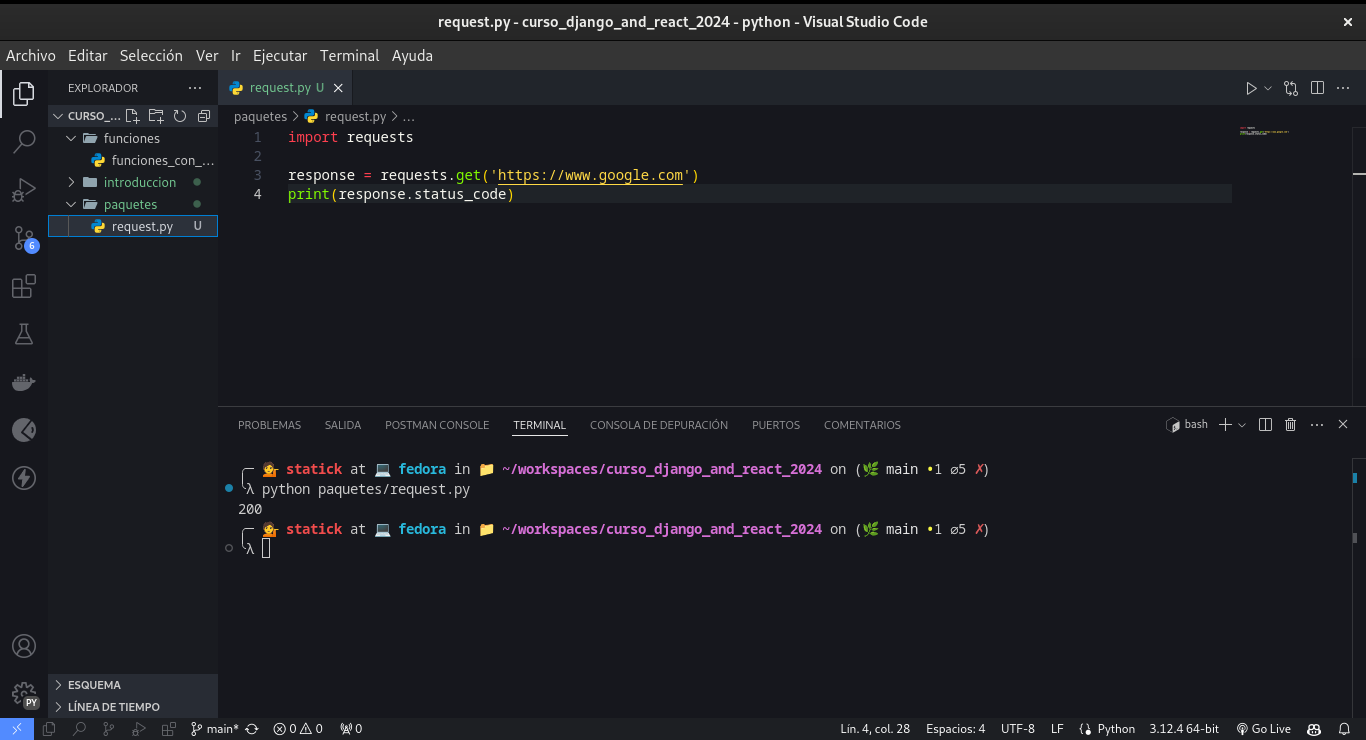
\includegraphics{unidades/unidad4/images/paste-1.png}

Para utilizar un paquete de Pypi, primero debes instalarlo usando
\textbf{pip}. Por ejemplo, si quieres instalar el paquete
\textbf{requests}, puedes hacerlo de la siguiente manera:

\begin{Shaded}
\begin{Highlighting}[]
\ExtensionTok{pip}\NormalTok{ install requests}
\end{Highlighting}
\end{Shaded}

Una vez que hayas instalado el paquete, puedes importarlo en tu código
de Python y utilizarlo. Por ejemplo:

\begin{Shaded}
\begin{Highlighting}[]
\ImportTok{import}\NormalTok{ requests}

\NormalTok{response }\OperatorTok{=}\NormalTok{ requests.get(}\StringTok{\textquotesingle{}https://www.google.com\textquotesingle{}}\NormalTok{)}
\BuiltInTok{print}\NormalTok{(response.status\_code)}
\end{Highlighting}
\end{Shaded}

Otro ejemplo es por ejemplo el paquete emoji, que te permite utilizar
emojis en tus programas de Python.

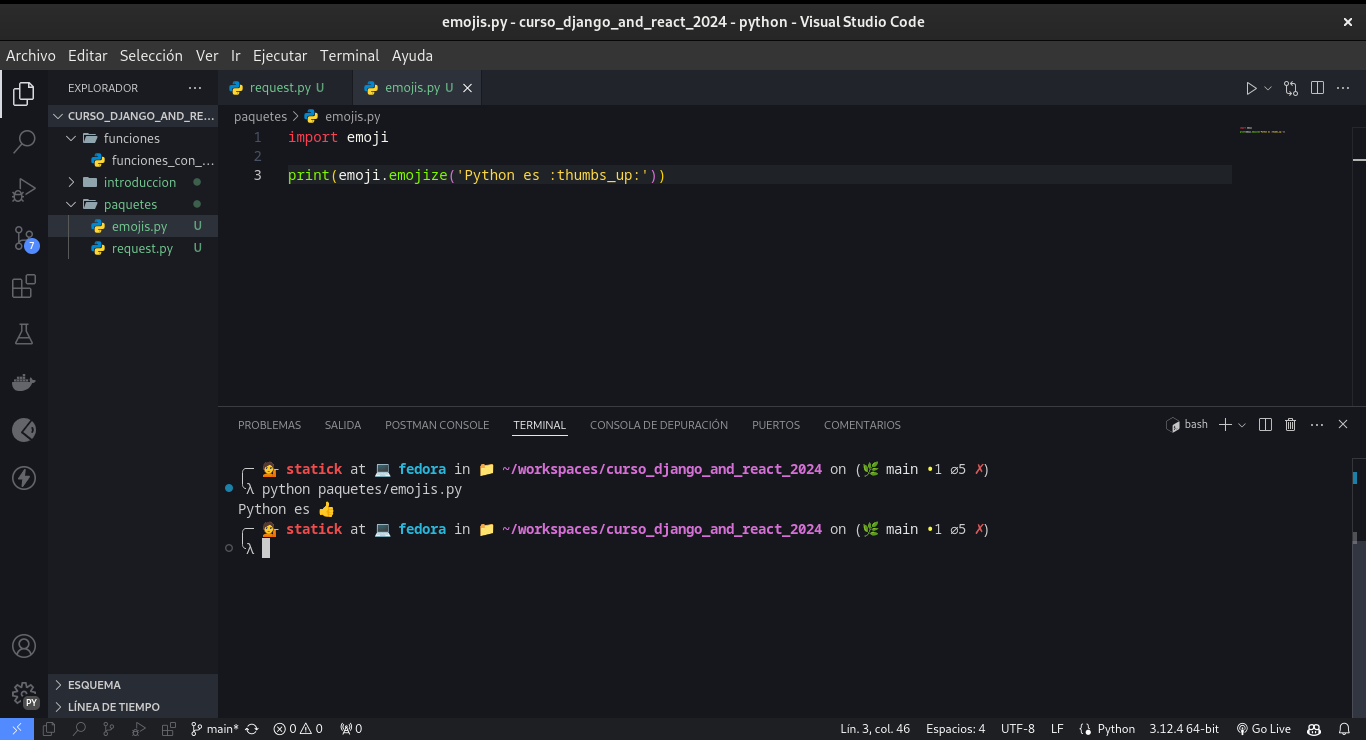
\includegraphics{unidades/unidad4/images/paste-2.png}

\begin{Shaded}
\begin{Highlighting}[]
\ExtensionTok{pip}\NormalTok{ install emoji}
\end{Highlighting}
\end{Shaded}

\begin{Shaded}
\begin{Highlighting}[]
\ImportTok{import}\NormalTok{ emoji}

\BuiltInTok{print}\NormalTok{(emoji.emojize(}\StringTok{\textquotesingle{}Python es :thumbs\_up:\textquotesingle{}}\NormalTok{))}
\end{Highlighting}
\end{Shaded}

¡Y eso es todo! Ahora puedes utilizar cualquier paquete de Python
disponible en Pypi en tus proyectos.

Algunos paquetes pueden ser muy importantes para tu proyecto, así que
asegúrate de revisar Pypi para encontrar los paquetes que necesitas.

\chapter{Conclusión}\label{conclusiuxf3n-1}

Pypi es un recurso valioso para los desarrolladores de Python. Te
permite compartir tus paquetes con otros desarrolladores y utilizar los
paquetes de otros desarrolladores en tus proyectos.

\chapter{Públicar un paquete en
Pypi}\label{puxfablicar-un-paquete-en-pypi}

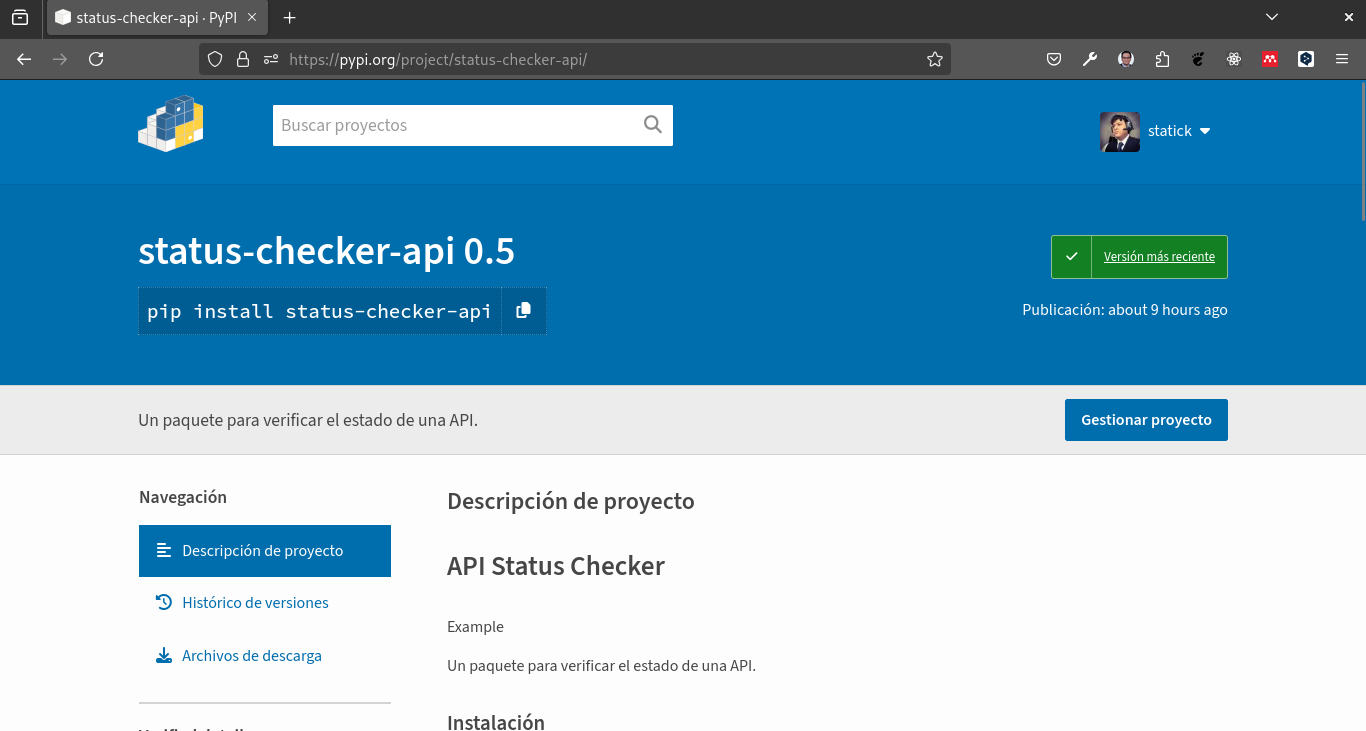
\includegraphics{unidades/unidad4/images/paste-10.png}

En este tutorial vamos a publicar un paquete llamado
\textbf{status-checker-api} en Pypi.

Si has creado un paquete de Python y quieres compartirlo con otros
desarrolladores, puedes publicarlo en Pypi.

Para ello vamos a crear un repositorio en \textbf{GitHub} y subir
nuestro paquete, esta práctica es importante para poder compartir
nuestro paquete con otros desarrolladores.

En el caso de este tutorial, el repositorio se encuentra en
\href{https://github.com/statick88/status_checker_api}{status\_checker\_api}

Lo más importante es tener el o los scripts que contienen el código que
queremos convertir a paquete.

Para ello vamos a empezar creando un directorio con el nombre de nuestro
paquete, por ejemplo \textbf{status\_checker\_api}.

A continuación se visualiza la estructura de nuestro paquete.

\begin{Shaded}
\begin{Highlighting}[]
\NormalTok{├── dist}
\NormalTok{│   ├── status\_checker\_api{-}0.5{-}py3{-}none{-}any.whl}
\NormalTok{│   └── status\_checker\_api{-}0.5.tar.gz}
\NormalTok{├── img}
\NormalTok{│   └── paste{-}5.png}
\NormalTok{├── LICENSE}
\NormalTok{├── README.md}
\NormalTok{├── setup.py}
\NormalTok{└── src}
\NormalTok{    ├── status\_checker\_api}
\NormalTok{    │   ├── \_\_init\_\_.py}
\NormalTok{    │   ├── \_\_main\_\_.py}
\NormalTok{    │   └── \_\_pycache\_\_}
\NormalTok{    │       ├── \_\_init\_\_.cpython{-}312.pyc}
\NormalTok{    │       └── \_\_main\_\_.cpython{-}312.pyc}
\NormalTok{    ├── status\_checker\_api.egg{-}info}
\NormalTok{    │   ├── dependency\_links.txt}
\NormalTok{    │   ├── entry\_points.txt}
\NormalTok{    │   ├── PKG{-}INFO}
\NormalTok{    │   ├── requires.txt}
\NormalTok{    │   ├── SOURCES.txt}
\NormalTok{    │   └── top\_level.txt}
\NormalTok{    └── tests}
\NormalTok{        ├── \_\_init\_\_.py}
\NormalTok{        ├── \_\_pycache\_\_}
\NormalTok{        │   ├── \_\_init\_\_.cpython{-}312.pyc}
\NormalTok{        │   └── test\_status\_checker\_api.cpython{-}312{-}pytest{-}8.3.2.pyc}
\NormalTok{        └── test\_status\_checker\_api.py}
\end{Highlighting}
\end{Shaded}

Dentro de este \textbf{status\_checker\_api} vamos a crear un directorio
llamado \textbf{src} y dentro de este directorio vamos a crear un
archivo llamado \textbf{\_\_init\_\_.py}, en este ejemplo tambien
crearemos el archivo \textbf{\_\_main\_\_.py}.

Para poder publicar nuestro paquete en Pypi, necesitamos crear un
archivo llamado \textbf{setup.py} en el directorio raíz de nuestro
paquete. Este archivo contiene la información necesaria para empaquetar
nuestro paquete y publicarlo en Pypi.

\begin{Shaded}
\begin{Highlighting}[]
\ImportTok{from}\NormalTok{ setuptools }\ImportTok{import}\NormalTok{ setup, find\_packages}

\ControlFlowTok{with} \BuiltInTok{open}\NormalTok{(}\StringTok{\textquotesingle{}README.md\textquotesingle{}}\NormalTok{, }\StringTok{\textquotesingle{}r\textquotesingle{}}\NormalTok{, encoding}\OperatorTok{=}\StringTok{"utf{-}8"}\NormalTok{) }\ImportTok{as}\NormalTok{ fh:}
\NormalTok{    long\_description }\OperatorTok{=}\NormalTok{ fh.read()}

\NormalTok{setup(}
\NormalTok{    name}\OperatorTok{=}\StringTok{\textquotesingle{}status\_checker\_api\textquotesingle{}}\NormalTok{,}
\NormalTok{    version}\OperatorTok{=}\StringTok{\textquotesingle{}0.5\textquotesingle{}}\NormalTok{,}
\NormalTok{    packages}\OperatorTok{=}\NormalTok{find\_packages(where}\OperatorTok{=}\StringTok{\textquotesingle{}src\textquotesingle{}}\NormalTok{),}
\NormalTok{    package\_dir}\OperatorTok{=}\NormalTok{\{}\StringTok{\textquotesingle{}\textquotesingle{}}\NormalTok{: }\StringTok{\textquotesingle{}src\textquotesingle{}}\NormalTok{\},}
\NormalTok{    install\_requires}\OperatorTok{=}\NormalTok{[}
        \StringTok{\textquotesingle{}requests\textquotesingle{}}\NormalTok{,}
\NormalTok{    ],}
\NormalTok{    entry\_points}\OperatorTok{=}\NormalTok{\{}
        \StringTok{\textquotesingle{}console\_scripts\textquotesingle{}}\NormalTok{: [}
            \StringTok{\textquotesingle{}status{-}checker{-}api=status\_checker\_api.\_\_main\_\_:main\textquotesingle{}}\NormalTok{,}
\NormalTok{        ],}
\NormalTok{    \},}
\NormalTok{    author}\OperatorTok{=}\StringTok{\textquotesingle{}Diego Saavedra\textquotesingle{}}\NormalTok{,}
\NormalTok{    author\_email}\OperatorTok{=}\StringTok{\textquotesingle{}dsaavedra88@gmail.com\textquotesingle{}}\NormalTok{,}
\NormalTok{    description}\OperatorTok{=}\StringTok{\textquotesingle{}Un paquete para verificar el estado de una API.\textquotesingle{}}\NormalTok{,}
\NormalTok{    long\_description}\OperatorTok{=}\NormalTok{long\_description,}
\NormalTok{    long\_description\_content\_type}\OperatorTok{=}\StringTok{\textquotesingle{}text/markdown\textquotesingle{}}\NormalTok{,}
\NormalTok{    url}\OperatorTok{=}\StringTok{\textquotesingle{}https://github.com/statick88/status\_checker\_api\textquotesingle{}}\NormalTok{,}
\NormalTok{    classifiers}\OperatorTok{=}\NormalTok{[}
        \StringTok{\textquotesingle{}Programming Language :: Python :: 3\textquotesingle{}}\NormalTok{,}
        \StringTok{\textquotesingle{}License :: OSI Approved :: MIT License\textquotesingle{}}\NormalTok{,}
        \StringTok{\textquotesingle{}Operating System :: OS Independent\textquotesingle{}}\NormalTok{,}
\NormalTok{    ],}
\NormalTok{    options}\OperatorTok{=}\NormalTok{\{}
        \StringTok{\textquotesingle{}egg\_info\textquotesingle{}}\NormalTok{: \{}
            \StringTok{\textquotesingle{}egg\_base\textquotesingle{}}\NormalTok{: }\StringTok{\textquotesingle{}src\textquotesingle{}}
\NormalTok{        \}}
\NormalTok{    \},}
\NormalTok{    python\_requires}\OperatorTok{=}\StringTok{\textquotesingle{}\textgreater{}=3.12\textquotesingle{}}\NormalTok{,}
\NormalTok{)}
\end{Highlighting}
\end{Shaded}

\chapter{Creación del archivo
README.md}\label{creaciuxf3n-del-archivo-readme.md}

\begin{Shaded}
\begin{Highlighting}[]
\FunctionTok{\# status\_checker\_api}

\NormalTok{Un paquete para verificar el estado de una API.}

\FunctionTok{\#\# Instalación}

\NormalTok{pip install status\_checker\_api}

\FunctionTok{\#\# Uso}

\NormalTok{api{-}status{-}checker}

\NormalTok{Ingrese la URL de la API: https://www.google.com}

\NormalTok{El status de la API es: 200}

\FunctionTok{\#\# Licencia}

\NormalTok{MIT License}

\FunctionTok{\#\# Autor}

\NormalTok{Diego Saavedra}
\end{Highlighting}
\end{Shaded}

El código del paquete se encuentra en el directorio \textbf{src}. Para
poder ejecutar el paquete, necesitamos un archivo llamado
\textbf{\_\_init\_\_.py} en el directorio \textbf{status\_checker\_api}.

\begin{Shaded}
\begin{Highlighting}[]
\ImportTok{import}\NormalTok{ requests}
\ImportTok{from}\NormalTok{ urllib.parse }\ImportTok{import}\NormalTok{ urlparse}

\KeywordTok{def}\NormalTok{ check\_status(url):}
    \CommentTok{\# Asegúrate de que la URL tenga un esquema (http o https)}
\NormalTok{    parsed\_url }\OperatorTok{=}\NormalTok{ urlparse(url)}
    \ControlFlowTok{if} \KeywordTok{not}\NormalTok{ parsed\_url.scheme:}
\NormalTok{        url }\OperatorTok{=} \StringTok{\textquotesingle{}https://\textquotesingle{}} \OperatorTok{+}\NormalTok{ url}
    
    \ControlFlowTok{try}\NormalTok{:}
\NormalTok{        response }\OperatorTok{=}\NormalTok{ requests.get(url)}
        \ControlFlowTok{return} \SpecialStringTok{f"La URL está activa con código de estado: }\SpecialCharTok{\{}\NormalTok{response}\SpecialCharTok{.}\NormalTok{status\_code}\SpecialCharTok{\}}\SpecialStringTok{"}  \CommentTok{\# Devuelve el mensaje con el código de estado}
    \ControlFlowTok{except}\NormalTok{ requests.exceptions.RequestException }\ImportTok{as}\NormalTok{ e:}
        \ControlFlowTok{return} \SpecialStringTok{f"Error: }\SpecialCharTok{\{}\NormalTok{e}\SpecialCharTok{\}}\SpecialStringTok{"}  \CommentTok{\# Devuelve el mensaje de error con una x}
\end{Highlighting}
\end{Shaded}

Analizando el código anterior, podemos ver que el paquete
\textbf{status\_checker\_api} contiene una función llamada
\textbf{check\_status} que verifica el estado de una API. La función
toma una URL como argumento y devuelve un mensaje con el estado de la
API.

\chapter{Creación del archivo
\_\_main\_\_.py}\label{creaciuxf3n-del-archivo-__main__.py}

\begin{Shaded}
\begin{Highlighting}[]
\ImportTok{from}\NormalTok{ status\_checker\_api }\ImportTok{import}\NormalTok{ check\_status}

\KeywordTok{def}\NormalTok{ main():}
\NormalTok{    url }\OperatorTok{=} \BuiltInTok{input}\NormalTok{(}\StringTok{\textquotesingle{}Ingrese la URL de la API: \textquotesingle{}}\NormalTok{)}
\NormalTok{    status }\OperatorTok{=}\NormalTok{ check\_status(url)}
    \BuiltInTok{print}\NormalTok{(}\SpecialStringTok{f\textquotesingle{}El status de la API es: }\SpecialCharTok{\{}\NormalTok{status}\SpecialCharTok{\}}\SpecialStringTok{\textquotesingle{}}\NormalTok{)}

\ControlFlowTok{if} \VariableTok{\_\_name\_\_} \OperatorTok{==} \StringTok{"\_\_main\_\_"}\NormalTok{:}
\NormalTok{    main()}
\end{Highlighting}
\end{Shaded}

El archivo \textbf{\_\_main\_\_.py} contiene el código principal del
paquete. Este archivo importa la función \textbf{check\_status} del
paquete \textbf{status\_checker\_api} y la utiliza para verificar el
estado de una API.

\chapter{Creación del archivo
LICENSE}\label{creaciuxf3n-del-archivo-license}

\begin{Shaded}
\begin{Highlighting}[]
\NormalTok{MIT License}

\NormalTok{Copyright (c) 2024 Diego Saavedra}

\NormalTok{Permission is hereby granted, free of charge, to any person obtaining a copy}
\NormalTok{of this software and associated documentation files (the "Software"), to deal}
\NormalTok{in the Software without restriction, including without limitation the rights}
\NormalTok{to use, copy, modify, merge, publish, distribute, sublicense, and/or sell}
\NormalTok{copies of the Software, and to permit persons to whom the Software is}
\NormalTok{furnished to do so, subject to the following conditions:}

\NormalTok{The above copyright notice and this permission notice shall be included in all}

\NormalTok{copies or substantial portions of the Software.}
\end{Highlighting}
\end{Shaded}

El archivo \textbf{LICENSE} contiene la licencia del paquete. En este
caso, utilizamos la licencia MIT.

\chapter{Creación del archivo
.gitignore}\label{creaciuxf3n-del-archivo-.gitignore}

\begin{Shaded}
\begin{Highlighting}[]
\NormalTok{\# Byte{-}compiled / optimized / DLL files}
\NormalTok{\_\_pycache\_\_/}
\NormalTok{*.py[cod]}
\NormalTok{*$py.class}

\NormalTok{\# C extensions}
\NormalTok{*.so}

\NormalTok{\# Distribution / packaging}
\NormalTok{dist/}
\NormalTok{build/}
\NormalTok{*.egg{-}info/}
\NormalTok{*.egg}

\NormalTok{\# Virtual environments}
\NormalTok{venv/}
\NormalTok{env/}
\NormalTok{ENV/}

\NormalTok{\# IDEs / Editors}
\NormalTok{.idea/}
\NormalTok{.vscode/}
\NormalTok{*.sublime{-}project}
\NormalTok{*.sublime{-}workspace}

\NormalTok{\# Miscellaneous}
\NormalTok{*.swp}
\NormalTok{.DS\_Store}
\end{Highlighting}
\end{Shaded}

El archivo \textbf{.gitignore} contiene los archivos y directorios que
no queremos incluir en nuestro repositorio de Git. En este caso,
ignoramos los archivos y directorios generados por Python y los entornos
virtuales.

\chapter{Creación de la cuenta en
Pypi}\label{creaciuxf3n-de-la-cuenta-en-pypi}

Para poder publicar nuestro paquete en Pypi, necesitamos crear una
cuenta en \href{https://pypi.org/account/register/}{Pypi}.

\begin{tcolorbox}[enhanced jigsaw, breakable, titlerule=0mm, colframe=quarto-callout-tip-color-frame, left=2mm, opacityback=0, rightrule=.15mm, colback=white, opacitybacktitle=0.6, title=\textcolor{quarto-callout-tip-color}{\faLightbulb}\hspace{0.5em}{Tip}, toprule=.15mm, bottomtitle=1mm, leftrule=.75mm, colbacktitle=quarto-callout-tip-color!10!white, toptitle=1mm, coltitle=black, arc=.35mm, bottomrule=.15mm]

Una vez creada la cuenta en Pypi, necesitamos verificarla a través de un
correo electrónico que nos enviarán. Adicional a ello es necesario
configurar un factor de doble autenticación. Esto es indispensable para
poder crear un token de acceso. El mismo que nos permitirá subir nuestro
paquete a Pypi.

\end{tcolorbox}

Una vez que hayamos creado la cuenta, necesitamos crear un archivo
llamado \textbf{.pypirc} en nuestro directorio de usuario con la
siguiente información:

\begin{Shaded}
\begin{Highlighting}[]
\NormalTok{[pypi]}
\NormalTok{  username = statick}
\NormalTok{  password = pypi{-}token}
\end{Highlighting}
\end{Shaded}

En el archivo \textbf{.pypirc}, reemplazamos \textbf{username} con
nuestro nombre de usuario de Pypi y \textbf{password} con nuestro token
de acceso de Pypi.

\begin{tcolorbox}[enhanced jigsaw, breakable, titlerule=0mm, colframe=quarto-callout-tip-color-frame, left=2mm, opacityback=0, rightrule=.15mm, colback=white, opacitybacktitle=0.6, title=\textcolor{quarto-callout-tip-color}{\faLightbulb}\hspace{0.5em}{Tip}, toprule=.15mm, bottomtitle=1mm, leftrule=.75mm, colbacktitle=quarto-callout-tip-color!10!white, toptitle=1mm, coltitle=black, arc=.35mm, bottomrule=.15mm]

En sistemas operativos basados en Unix, el archivo \textbf{.pypirc} se
encuentra en el directorio de usuario \textbf{.pypirc}.

En sistemas operativos basados en Windows, el archivo \textbf{.pypirc}
se encuentra en el directorio de usuario \textbf{C:} / Users / username
/ --\textgreater{} en este directorio se almacena el archivo
\textbf{.pypirc}.

\end{tcolorbox}

\chapter{Publicar el paquete en Pypi}\label{publicar-el-paquete-en-pypi}

Para publicar nuestro paquete en Pypi, necesitamos instalar el paquete
\textbf{twine}.

Twine es una herramienta que nos permite subir paquetes de Python a
Pypi.

\begin{Shaded}
\begin{Highlighting}[]
\ExtensionTok{pip}\NormalTok{ install twine}
\end{Highlighting}
\end{Shaded}

Es recomandable que tengamos la última versión de \textbf{twine}.

\begin{Shaded}
\begin{Highlighting}[]
\ExtensionTok{pip}\NormalTok{ install }\AttributeTok{{-}{-}upgrade}\NormalTok{ twine}
\end{Highlighting}
\end{Shaded}

Una vez que hayamos instalado y actualizado \textbf{twine}, podemos
publicar nuestro paquete en Pypi de la siguiente manera:

\begin{Shaded}
\begin{Highlighting}[]
\ExtensionTok{python} \AttributeTok{{-}m}\NormalTok{ pip install }\AttributeTok{{-}{-}upgrade}\NormalTok{ build}
\end{Highlighting}
\end{Shaded}

El comando anterior instala el paquete \textbf{build} que necesitamos
para construir nuestro paquete.

\begin{Shaded}
\begin{Highlighting}[]
\ExtensionTok{python} \AttributeTok{{-}m}\NormalTok{ build}
\end{Highlighting}
\end{Shaded}

El comando anterior crea un archivo \textbf{dist} en el directorio raíz
de nuestro paquete. Este archivo contiene el paquete que vamos a
publicar en Pypi. Es decir los archivos \textbf{.tar.gz} y
\textbf{.whl}.

Estos archivos son los que vamos a subir a Pypi.

\begin{Shaded}
\begin{Highlighting}[]
\ExtensionTok{python} \AttributeTok{{-}m}\NormalTok{ twine upload }\AttributeTok{{-}{-}repository}\NormalTok{ pypi dist/}\PreprocessorTok{*} \AttributeTok{{-}{-}verbose}
\end{Highlighting}
\end{Shaded}

El comando anterior sube nuestro paquete a Pypi. El archivo
\textbf{.pypirc} contiene la información de autenticación que
necesitamos para subir nuestro paquete.

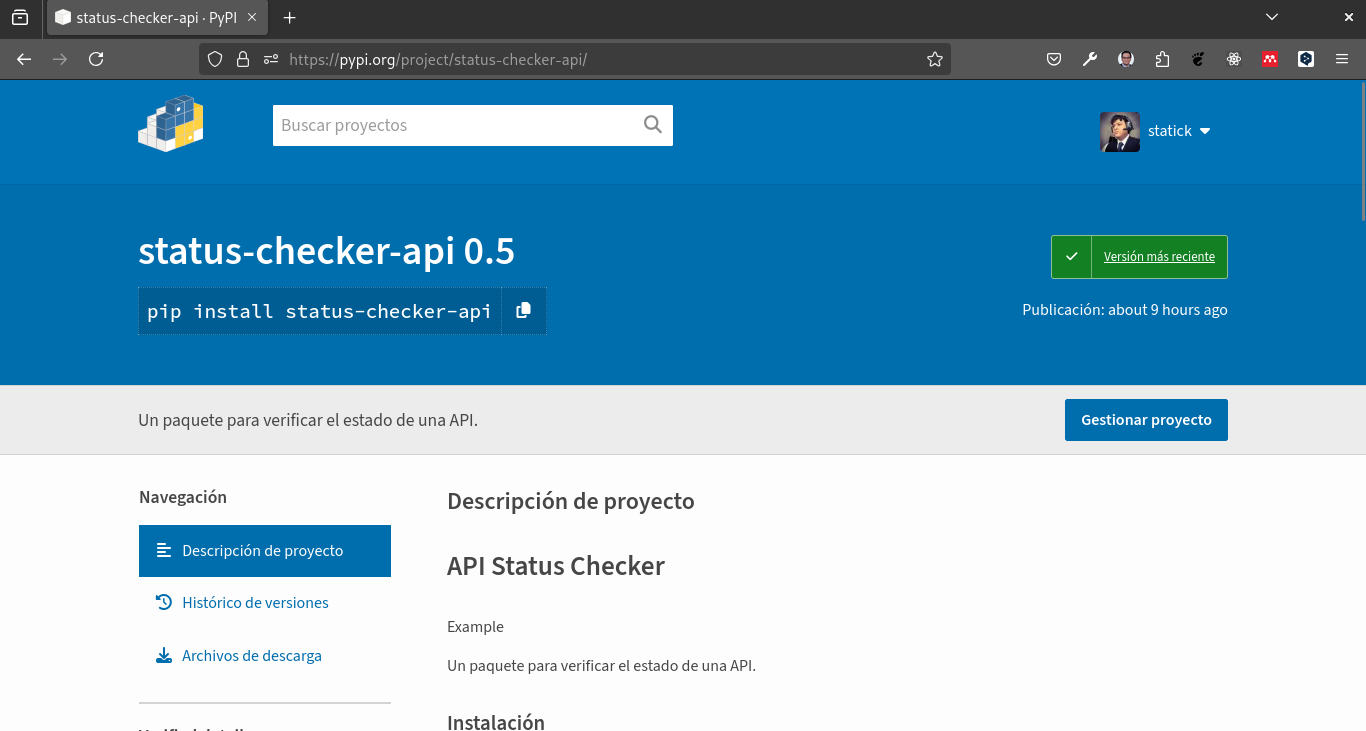
\includegraphics{unidades/unidad4/images/paste-10.png}

¡Y eso es todo! Ahora puedes compartir tu paquete de Python con otros
desarrolladores en Pypi. En el caso de este paquete la url es
\href{https://pypi.org/project/status-checker-api/}{status\_checker\_api}.

\chapter{Instalar el paquete}\label{instalar-el-paquete}

Para instalar el paquete que acabamos de publicar en Pypi, necesitamos
usar \textbf{pip}.

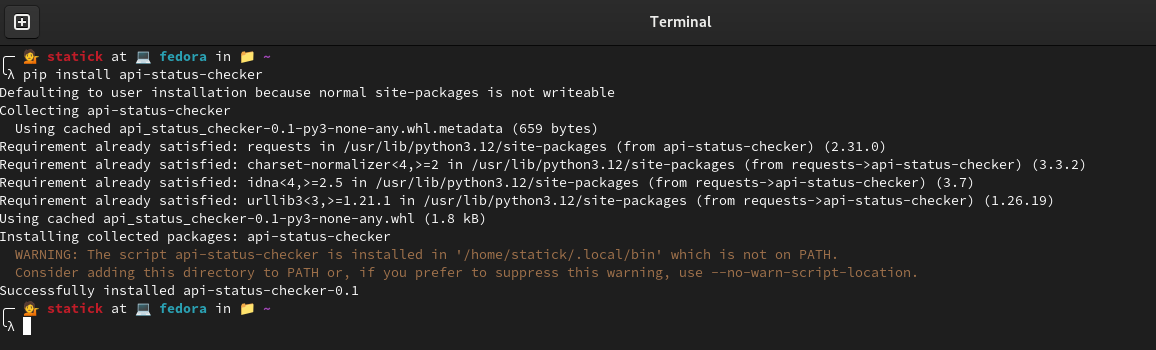
\includegraphics{unidades/unidad4/images/paste-4.png}

\begin{Shaded}
\begin{Highlighting}[]
\ExtensionTok{pip}\NormalTok{ install status\_checker\_api}
\end{Highlighting}
\end{Shaded}

Una vez que hayamos instalado el paquete, podemos utilizarlo en nuestro
código de Python.

\chapter{Uso del paquete}\label{uso-del-paquete}

\begin{Shaded}
\begin{Highlighting}[]
\ExtensionTok{api{-}status{-}checker}
\end{Highlighting}
\end{Shaded}

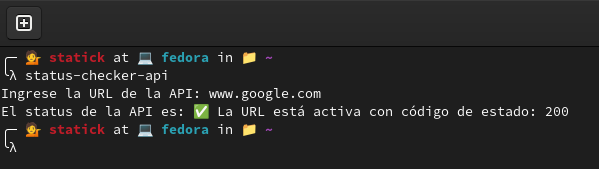
\includegraphics{unidades/unidad4/images/paste-11.png}

Es necesario ingresar la URL de la API que queremos verificar.

\textbf{Ingrese la URL de la API:} https://www.google.com

\textbf{El status de la API es:} 200

¡Y eso es todo! Ahora puedes actualizar tu paquete de Python en Pypi.

\begin{tcolorbox}[enhanced jigsaw, breakable, titlerule=0mm, colframe=quarto-callout-tip-color-frame, left=2mm, opacityback=0, rightrule=.15mm, colback=white, opacitybacktitle=0.6, title=\textcolor{quarto-callout-tip-color}{\faLightbulb}\hspace{0.5em}{Tip}, toprule=.15mm, bottomtitle=1mm, leftrule=.75mm, colbacktitle=quarto-callout-tip-color!10!white, toptitle=1mm, coltitle=black, arc=.35mm, bottomrule=.15mm]

No olvides cambiar la versión de tu paquete en el archivo
\textbf{setup.py} antes de subirlo a Pypi si realizas alguna
actualización.

\end{tcolorbox}

Si decidimos actualizar el paquete en Pypi, necesitamos seguir los
mismos pasos que hemos visto en este tutorial.

Sin embargo solo necesitaremos 2 comandos:

\begin{Shaded}
\begin{Highlighting}[]
\ExtensionTok{python} \AttributeTok{{-}m}\NormalTok{ build}
\end{Highlighting}
\end{Shaded}

\begin{Shaded}
\begin{Highlighting}[]
\ExtensionTok{python} \AttributeTok{{-}m}\NormalTok{ twine upload }\AttributeTok{{-}{-}repository}\NormalTok{ pypi dist/}\PreprocessorTok{*} \AttributeTok{{-}{-}verbose}
\end{Highlighting}
\end{Shaded}

\begin{tcolorbox}[enhanced jigsaw, breakable, titlerule=0mm, colframe=quarto-callout-tip-color-frame, left=2mm, opacityback=0, rightrule=.15mm, colback=white, opacitybacktitle=0.6, title=\textcolor{quarto-callout-tip-color}{\faLightbulb}\hspace{0.5em}{Tip}, toprule=.15mm, bottomtitle=1mm, leftrule=.75mm, colbacktitle=quarto-callout-tip-color!10!white, toptitle=1mm, coltitle=black, arc=.35mm, bottomrule=.15mm]

En el directorio dist se generan los archivos \textbf{.tar.gz} y
\textbf{.whl} que son los que vamos a subir a Pypi. Es necesario
eliminar los archivos anteriores antes de subir los nuevos en este
directorio, mi recomendación es eliminar el directorio \textbf{dist} y
volver a ejecutar el comando \textbf{python -m build}.

\end{tcolorbox}

\chapter{Conclusión}\label{conclusiuxf3n-2}

En este tutorial aprendimos cómo publicar un paquete de Python en Pypi.
Pudimos ver cómo crear un paquete de Python, subirlo a Pypi y
compartirlo con otros desarrolladores.

\chapter{Desarrollo de un Sistema de Gestión de Inventarios en
Python}\label{desarrollo-de-un-sistema-de-gestiuxf3n-de-inventarios-en-python}

Este laboratorio tiene como objetivo guiarte en el desarrollo de un
sistema de gestión de inventarios utilizando el lenguaje de programación
Python. A través de esta actividad, aprenderás a implementar
funcionalidades clave en un proyecto práctico que puedes utilizar como
base para futuros desarrollos.

\section{Objetivos}\label{objetivos}

\begin{itemize}
\item
  \textbf{Diseño de la estructura de datos:} Aprenderás a diseñar y
  crear una estructura de datos para almacenar la información de los
  productos, incluyendo atributos como nombre, descripción, precio, y
  cantidad disponible.
\item
  \textbf{Agregar productos:} Implementarás la funcionalidad para
  agregar nuevos productos al inventario.
\item
  \textbf{Búsqueda y filtrado:} Aprenderás a implementar funciones de
  búsqueda y filtrado para encontrar productos específicos basados en
  diferentes criterios.
\item
  \textbf{Actualización de inventario:} Desarrollarás funciones para
  manejar la compra y venta de productos, permitiendo ajustar la
  cantidad disponible en el inventario.
\item
  \textbf{Generación de informes:} Crearás funciones para generar
  informes sobre el estado del inventario, tales como productos
  disponibles, productos más vendidos, y productos con bajo stock.
\end{itemize}

\section{Entregables}\label{entregables}

\begin{itemize}
\tightlist
\item
  \textbf{Código fuente del proyecto:} Estructurado y organizado de
  manera coherente.
\item
  \textbf{Documentación del proyecto:} Incluyendo instrucciones de
  instalación, uso, y una breve explicación del diseño de la solución
  (Esto se sugiere generar en el \textbf{Readme.md} del proyecto).
\item
  \textbf{Pruebas unitarias:} Implementación de pruebas para verificar
  que las funcionalidades clave del sistema funcionan correctamente.
\end{itemize}

\section{Instrucciones}\label{instrucciones-2}

\subsection{1. Crear la Estructura de
Datos}\label{crear-la-estructura-de-datos}

Diseña una clase Producto que contenga los atributos básicos como
nombre, descripción, precio, y cantidad disponible. Implementa un método
\textbf{str} para imprimir la información del producto de manera
legible.

Solución

\begin{Shaded}
\begin{Highlighting}[]
\KeywordTok{class}\NormalTok{ Producto:}
    \KeywordTok{def} \FunctionTok{\_\_init\_\_}\NormalTok{(}\VariableTok{self}\NormalTok{, nombre, descripcion, precio, cantidad):}
        \VariableTok{self}\NormalTok{.nombre }\OperatorTok{=}\NormalTok{ nombre}
        \VariableTok{self}\NormalTok{.descripcion }\OperatorTok{=}\NormalTok{ descripcion}
        \VariableTok{self}\NormalTok{.precio }\OperatorTok{=}\NormalTok{ precio}
        \VariableTok{self}\NormalTok{.cantidad }\OperatorTok{=}\NormalTok{ cantidad}

    \KeywordTok{def} \FunctionTok{\_\_str\_\_}\NormalTok{(}\VariableTok{self}\NormalTok{):}
        \ControlFlowTok{return} \SpecialStringTok{f"Producto: }\SpecialCharTok{\{}\VariableTok{self}\SpecialCharTok{.}\NormalTok{nombre}\SpecialCharTok{\}}\SpecialStringTok{, Precio: }\SpecialCharTok{\{}\VariableTok{self}\SpecialCharTok{.}\NormalTok{precio}\SpecialCharTok{\}}\SpecialStringTok{, Cantidad: }\SpecialCharTok{\{}\VariableTok{self}\SpecialCharTok{.}\NormalTok{cantidad}\SpecialCharTok{\}}\SpecialStringTok{"}
\end{Highlighting}
\end{Shaded}

\subsection{2. Agregar Productos}\label{agregar-productos}

Implementa una función que permita agregar nuevos productos a una lista
que actúe como el inventario.

Solución

\begin{Shaded}
\begin{Highlighting}[]
\NormalTok{inventario }\OperatorTok{=}\NormalTok{ []}

\KeywordTok{def}\NormalTok{ agregar\_producto(producto):}
\NormalTok{    inventario.append(producto)}
    \BuiltInTok{print}\NormalTok{(}\SpecialStringTok{f"}\SpecialCharTok{\{}\NormalTok{producto}\SpecialCharTok{.}\NormalTok{nombre}\SpecialCharTok{\}}\SpecialStringTok{ ha sido añadido al inventario."}\NormalTok{)}
\end{Highlighting}
\end{Shaded}

\subsection{3. Búsqueda y Filtrado}\label{buxfasqueda-y-filtrado}

Crea funciones para buscar productos por nombre, categoría o rango de
precios.

Solución

\begin{Shaded}
\begin{Highlighting}[]
\KeywordTok{def}\NormalTok{ buscar\_producto\_por\_nombre(nombre):}
    \ControlFlowTok{return}\NormalTok{ [p }\ControlFlowTok{for}\NormalTok{ p }\KeywordTok{in}\NormalTok{ inventario }\ControlFlowTok{if}\NormalTok{ nombre.lower() }\KeywordTok{in}\NormalTok{ p.nombre.lower()]}

\KeywordTok{def}\NormalTok{ buscar\_producto\_por\_precio(min\_precio, max\_precio):}
    \ControlFlowTok{return}\NormalTok{ [p }\ControlFlowTok{for}\NormalTok{ p }\KeywordTok{in}\NormalTok{ inventario }\ControlFlowTok{if}\NormalTok{ min\_precio }\OperatorTok{\textless{}=}\NormalTok{ p.precio }\OperatorTok{\textless{}=}\NormalTok{ max\_precio]}
\end{Highlighting}
\end{Shaded}

\subsection{4. Actualización de
Inventario}\label{actualizaciuxf3n-de-inventario}

Implementa funciones para aumentar o disminuir la cantidad de productos
en el inventario, simulando la compra o venta de productos.

Solución

\begin{Shaded}
\begin{Highlighting}[]
\KeywordTok{def}\NormalTok{ actualizar\_cantidad(nombre, cantidad):}
    \ControlFlowTok{for}\NormalTok{ producto }\KeywordTok{in}\NormalTok{ inventario:}
        \ControlFlowTok{if}\NormalTok{ producto.nombre }\OperatorTok{==}\NormalTok{ nombre:}
\NormalTok{            producto.cantidad }\OperatorTok{+=}\NormalTok{ cantidad}
            \BuiltInTok{print}\NormalTok{(}\SpecialStringTok{f"Cantidad actualizada: }\SpecialCharTok{\{}\NormalTok{producto}\SpecialCharTok{.}\NormalTok{nombre}\SpecialCharTok{\}}\SpecialStringTok{ ahora tiene }\SpecialCharTok{\{}\NormalTok{producto}\SpecialCharTok{.}\NormalTok{cantidad}\SpecialCharTok{\}}\SpecialStringTok{ unidades."}\NormalTok{)}
            \ControlFlowTok{return}
    \BuiltInTok{print}\NormalTok{(}\StringTok{"Producto no encontrado."}\NormalTok{)}
\end{Highlighting}
\end{Shaded}

\subsection{5. Generación de Informes}\label{generaciuxf3n-de-informes}

Crea funciones para generar informes del estado del inventario.

Solución

\begin{Shaded}
\begin{Highlighting}[]
\KeywordTok{def}\NormalTok{ generar\_informe\_productos\_disponibles():}
    \ControlFlowTok{return}\NormalTok{ [p }\ControlFlowTok{for}\NormalTok{ p }\KeywordTok{in}\NormalTok{ inventario }\ControlFlowTok{if}\NormalTok{ p.cantidad }\OperatorTok{\textgreater{}} \DecValTok{0}\NormalTok{]}

\KeywordTok{def}\NormalTok{ generar\_informe\_productos\_bajo\_stock(limite):}
    \ControlFlowTok{return}\NormalTok{ [p }\ControlFlowTok{for}\NormalTok{ p }\KeywordTok{in}\NormalTok{ inventario }\ControlFlowTok{if}\NormalTok{ p.cantidad }\OperatorTok{\textless{}=}\NormalTok{ limite]}
\end{Highlighting}
\end{Shaded}

\subsection{6. Pruebas Unitarias}\label{pruebas-unitarias}

Escribe pruebas para cada una de las funciones clave utilizando
unittest.

Solución

\begin{Shaded}
\begin{Highlighting}[]
\ImportTok{import}\NormalTok{ unittest}

\KeywordTok{class}\NormalTok{ TestInventario(unittest.TestCase):}
    \KeywordTok{def}\NormalTok{ test\_agregar\_producto(}\VariableTok{self}\NormalTok{):}
\NormalTok{        producto }\OperatorTok{=}\NormalTok{ Producto(}\StringTok{"Test"}\NormalTok{, }\StringTok{"Descripcion"}\NormalTok{, }\FloatTok{10.0}\NormalTok{, }\DecValTok{5}\NormalTok{)}
\NormalTok{        agregar\_producto(producto)}
        \VariableTok{self}\NormalTok{.assertIn(producto, inventario)}
\end{Highlighting}
\end{Shaded}

\subsection{7. Documentación y GitHub
Classroom}\label{documentaciuxf3n-y-github-classroom}

Documenta el código fuente, incluyendo instrucciones sobre cómo ejecutar
el programa y las pruebas.

Configura tu repositorio de GitHub Classroom y sube todo el código y
documentación.

\subsection{Evaluación}\label{evaluaciuxf3n}

\begin{enumerate}
\def\labelenumi{\arabic{enumi}.}
\item
  \textbf{Funcionalidad (40\%):} El sistema implementa correctamente las
  funcionalidades solicitadas.
\item
  \textbf{Calidad del Código (30\%):} El código es claro, bien
  estructurado, y sigue buenas prácticas de programación.
\item
  \textbf{Pruebas (20\%):} Las pruebas cubren las funcionalidades clave
  y se ejecutan correctamente.
\item
  \textbf{Documentación (10\%):} La documentación es clara y proporciona
  una guía adecuada para el usuario.
\end{enumerate}

¡Buena suerte!

\section{Asignación}\label{asignaciuxf3n-5}

\url{https://classroom.github.com/a/OVCpAmrV}

Aprenderás a desarrollar un proyecto de utilizando el lenguaje de
programación Python.

Un sistema de gestión de inventarios es una herramienta que permite
realizar un seguimiento y control de los productos o artículos
almacenados en un negocio o empresa.

Aprenderás a utilizar diferentes conceptos y técnicas de programación
para implementar las funcionalidades clave de este sistema.

Algunas de las funcionalidades que implementaremos incluyen:

Aprenderás a crear una estructura de datos para almacenar la información
de los productos, como su nombre, descripción, precio, cantidad
disponible, etc. También aprenderás a agregar nuevos productos al
sistema.

Te enseñaré cómo implementar funciones de búsqueda y filtrado para
encontrar productos específicos en base a diferentes criterios, como el
nombre, la categoría o el precio.

Aprenderás a manejar las actualizaciones de inventario, como la compra o
venta de productos. Implementaremos funciones que permitan aumentar o
disminuir la cantidad disponible de un producto y mantener un registro
de estas transacciones.

Te mostraré cómo generar informes sobre el estado del inventario, como
la lista de productos disponibles, los productos más vendidos, los
productos con bajo stock, etc. Utilizaremos técnicas de manipulación de
datos y generación de informes para presentar esta información de manera
clara y concisa.

\end{tcolorbox}

\part{Unidad 5: Django}

\chapter{Introducción a Django}\label{introducciuxf3n-a-django}

\begin{figure}[H]

{\centering 
\includegraphics[width=2.08333in,height=\textheight]{images/django-logo.png}

}

\caption{Django Framework}

\end{figure}%

Django es un framework web de alto nivel que fomenta el desarrollo
rápido y limpio. Es un framework web de alto nivel que fomenta el
desarrollo rápido y limpio. Diseñado por desarrolladores experimentados,
Django se encarga de gran parte de la molestia del desarrollo web, por
lo que puedes concentrarte en escribir tu aplicación sin necesidad de
reinventar la rueda. Es gratuito y de código abierto, tiene una
comunidad activa y amigable, y es utilizado por algunas de las mayores
empresas del mundo.

\section{Conceptos Importantes}\label{conceptos-importantes}

\begin{tcolorbox}[enhanced jigsaw, breakable, titlerule=0mm, colframe=quarto-callout-tip-color-frame, left=2mm, opacityback=0, rightrule=.15mm, colback=white, opacitybacktitle=0.6, title=\textcolor{quarto-callout-tip-color}{\faLightbulb}\hspace{0.5em}{Tip}, toprule=.15mm, bottomtitle=1mm, leftrule=.75mm, colbacktitle=quarto-callout-tip-color!10!white, toptitle=1mm, coltitle=black, arc=.35mm, bottomrule=.15mm]

Antes de iniciar con Django es necesario conocer el concepto de
\textbf{Entornos Virtuales}.

\end{tcolorbox}

\subsection{Entornos Virtuales}\label{entornos-virtuales}

\begin{figure}[H]

{\centering 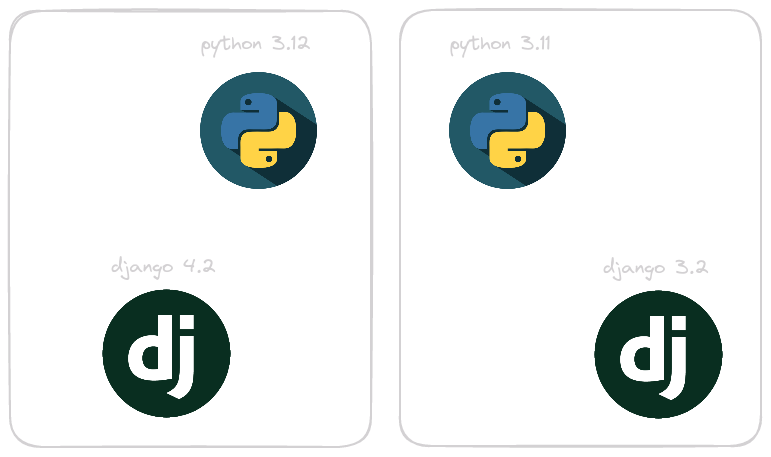
\includegraphics[width=4.16667in,height=\textheight]{images/python-venv.png}

}

\caption{Virtual Enviroment}

\end{figure}%

Un entorno virtual es un \textbf{entorno de desarrollo aislado }que
permite \textbf{instalar paquetes de Python sin afectar al sistema
global}. Los entornos virtuales son útiles para gestionar las
dependencias de un proyecto y para evitar conflictos entre diferentes
versiones de los paquetes.

\subsubsection{Crear un entorno virtual}\label{crear-un-entorno-virtual}

Para crear un entorno virtual, se puede utilizar la herramienta
\textbf{venv} de Python.

\begin{Shaded}
\begin{Highlighting}[]
\ExtensionTok{python} \AttributeTok{{-}m}\NormalTok{ venv env}
\end{Highlighting}
\end{Shaded}

Este comando creará un directorio llamado \textbf{env} en el directorio
actual con el entorno virtual.

\begin{tcolorbox}[enhanced jigsaw, breakable, titlerule=0mm, colframe=quarto-callout-tip-color-frame, left=2mm, opacityback=0, rightrule=.15mm, colback=white, opacitybacktitle=0.6, title=\textcolor{quarto-callout-tip-color}{\faLightbulb}\hspace{0.5em}{Tip}, toprule=.15mm, bottomtitle=1mm, leftrule=.75mm, colbacktitle=quarto-callout-tip-color!10!white, toptitle=1mm, coltitle=black, arc=.35mm, bottomrule=.15mm]

Tambien se puede utilizar
\href{https://pypi.org/project/virtualenv/}{virtualenv} para crear
entornos virtuales.

\end{tcolorbox}

\subsection{Modelo Template View (MTV)}\label{modelo-template-view-mtv}

\begin{figure}[H]

{\centering 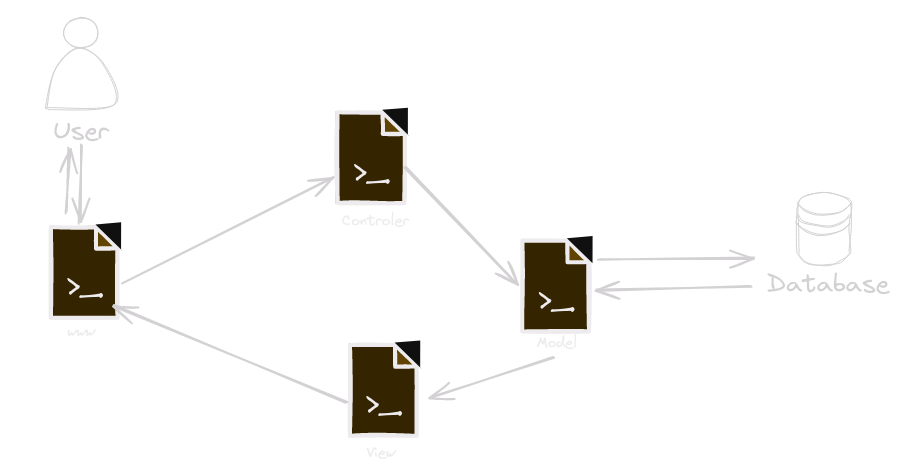
\includegraphics[width=4.16667in,height=\textheight]{images/model-view-controller.png}

}

\caption{Model View Controller}

\end{figure}%

\begin{figure}[H]

{\centering 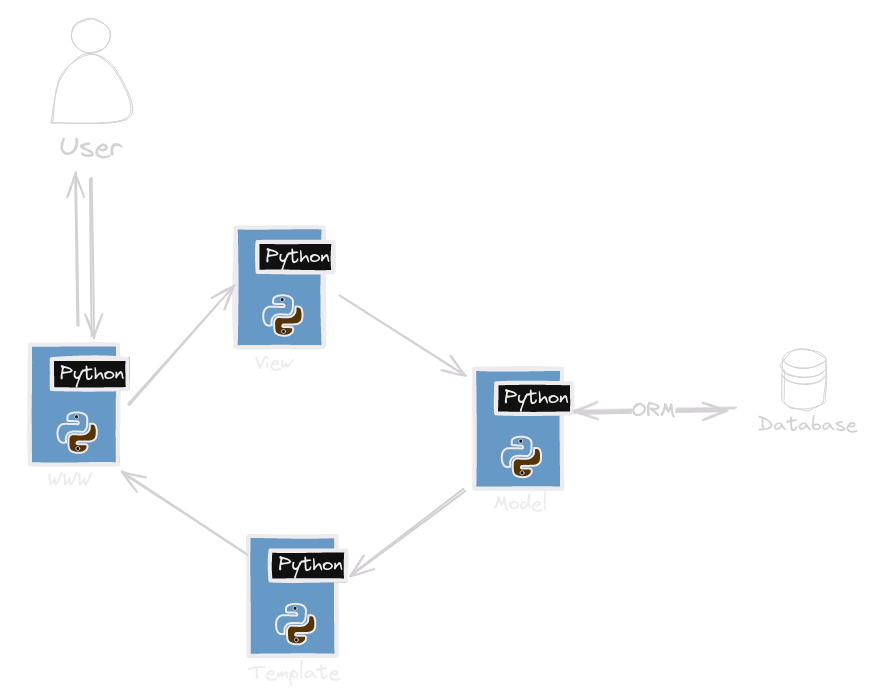
\includegraphics[width=4.16667in,height=\textheight]{images/model-template-view.png}

}

\caption{Model View Template}

\end{figure}%

Django sigue el patrón de diseño Modelo Vista Template (MVT). Este
patrón de diseño separa la lógica de la aplicación en tres componentes
principales: Modelo, Vista y Template.

\begin{tcolorbox}[enhanced jigsaw, breakable, titlerule=0mm, colframe=quarto-callout-tip-color-frame, left=2mm, opacityback=0, rightrule=.15mm, colback=white, opacitybacktitle=0.6, title=\textcolor{quarto-callout-tip-color}{\faLightbulb}\hspace{0.5em}{Tip}, toprule=.15mm, bottomtitle=1mm, leftrule=.75mm, colbacktitle=quarto-callout-tip-color!10!white, toptitle=1mm, coltitle=black, arc=.35mm, bottomrule=.15mm]

El archivo URLs.py es el encargado de mapear las URLs de la aplicación a
las vistas correspondientes.

\end{tcolorbox}

\begin{itemize}
\item
  \textbf{Modelo}: Es la representación de los datos de la aplicación y
  las reglas para manipular esos datos. Django utiliza un ORM
  (Object-Relational Mapping) para interactuar con la base de datos.
\item
  \textbf{Vista}: Es la capa de presentación de la aplicación. Se
  encarga de mostrar los datos al usuario y de interpretar las acciones
  del usuario.
\item
  \textbf{Template}: Es la capa de presentación de la aplicación. Define
  cómo se muestra la información al usuario. Django utiliza el motor de
  plantillas Jinja2 para renderizar los templates.
\end{itemize}

\subsection{Formularios}\label{formularios}

\begin{figure}[H]

{\centering 
\includegraphics{images/python-form.png}

}

\caption{Django Forms}

\end{figure}%

Los formularios son una parte importante de cualquier aplicación web.
Django proporciona una forma sencilla de crear y procesar formularios en
las vistas.

\subsection{Administrador de Django}\label{administrador-de-django}

\begin{figure}[H]

{\centering 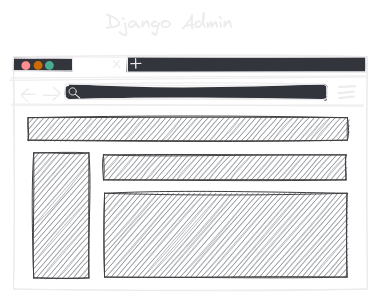
\includegraphics{images/django-admin.png}

}

\caption{Django Admin}

\end{figure}%

El administrador de Django es una interfaz de administración que permite
gestionar los datos de la aplicación de forma sencilla. Django genera
automáticamente una interfaz de administración basada en los modelos de
la aplicación.

\subsection{Middleware}\label{middleware}

El middleware es una capa de procesamiento que se ejecuta antes y
después de cada petición HTTP. Django proporciona un conjunto de
middlewares que se pueden utilizar para añadir funcionalidades a la
aplicación.

\subsection{Autenticación y
Autorización}\label{autenticaciuxf3n-y-autorizaciuxf3n}

Django proporciona un sistema de autenticación y autorización que
permite gestionar los usuarios y los permisos de la aplicación de forma
sencilla.

\subsection{Internacionalización}\label{internacionalizaciuxf3n}

Django proporciona soporte para la internacionalización de la
aplicación. Permite traducir la aplicación a diferentes idiomas y
gestionar las traducciones de forma sencilla.

\subsection{Seguridad}\label{seguridad}

Django proporciona un conjunto de medidas de seguridad para proteger la
aplicación contra ataques comunes, como la inyección de SQL, la
falsificación de solicitudes entre sitios (CSRF) y la inyección de
código.

\subsection{Testing}\label{testing}

Django proporciona un conjunto de herramientas para realizar pruebas
unitarias y de integración en la aplicación. Permite probar la lógica de
la aplicación y asegurarse de que funciona correctamente.

\subsection{Despliegue}\label{despliegue}

Django proporciona un conjunto de herramientas para desplegar la
aplicación en un servidor de producción. Permite configurar el entorno
de producción y gestionar las actualizaciones de la aplicación de forma
sencilla.

\chapter{Configuración inicial de un
proyecto.}\label{configuraciuxf3n-inicial-de-un-proyecto.}

\section{1. Crear un entorno virtual}\label{crear-un-entorno-virtual-1}

\begin{figure}[H]

{\centering 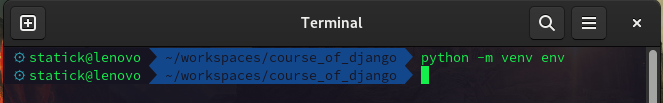
\includegraphics{images/creacion_entorno_virtual.png}

}

\caption{Creación de entorno Virtual}

\end{figure}%

\begin{Shaded}
\begin{Highlighting}[]
\ExtensionTok{python3} \AttributeTok{{-}m}\NormalTok{ venv env}
\end{Highlighting}
\end{Shaded}

El comando anterior creará un directorio llamado \textbf{env} en el
directorio actual, que contendrá un entorno virtual de Python.

\section{2. Activar el entorno
virtual}\label{activar-el-entorno-virtual}

\begin{figure}[H]

{\centering 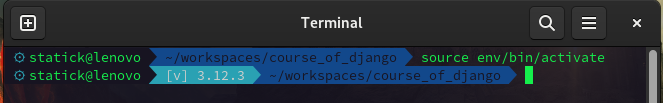
\includegraphics{images/activacion_entorno_virtual.png}

}

\caption{Activación de entorno Virtual}

\end{figure}%

\begin{Shaded}
\begin{Highlighting}[]
\BuiltInTok{source}\NormalTok{ env/bin/activate}
\end{Highlighting}
\end{Shaded}

El comando anterior activará el entorno virtual en sistemas Unix. En
Windows, el comando es:

\begin{Shaded}
\begin{Highlighting}[]
\FunctionTok{env}\DataTypeTok{\textbackslash{}S}\NormalTok{cripts}\DataTypeTok{\textbackslash{}a}\NormalTok{ctivate}
\end{Highlighting}
\end{Shaded}

Este comando tambien se puede dividir en 2 partes:

\begin{Shaded}
\begin{Highlighting}[]
\BuiltInTok{cd}\NormalTok{ env/Scripts/}
\ExtensionTok{activate}
\end{Highlighting}
\end{Shaded}

Para desactivar el entorno virtual, simplemente ejecute:

\begin{Shaded}
\begin{Highlighting}[]
\ExtensionTok{deactivate}
\end{Highlighting}
\end{Shaded}

\section{3. Instalar Django}\label{instalar-django}

\begin{figure}[H]

{\centering 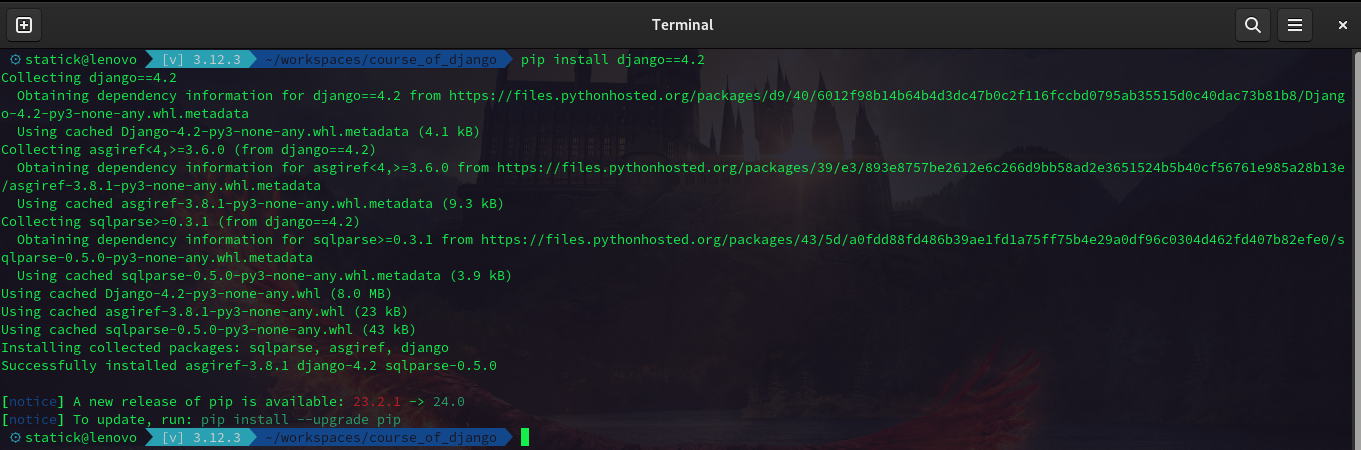
\includegraphics{images/instalacion_django.png}

}

\caption{Instalación de Django}

\end{figure}%

\begin{Shaded}
\begin{Highlighting}[]
\ExtensionTok{pip}\NormalTok{ install django==4.2}
\end{Highlighting}
\end{Shaded}

El comando anterior instalará la última versión de Django en el entorno
virtual.

\section{4. Crear un proyecto de
Django}\label{crear-un-proyecto-de-django}

\begin{figure}[H]

{\centering 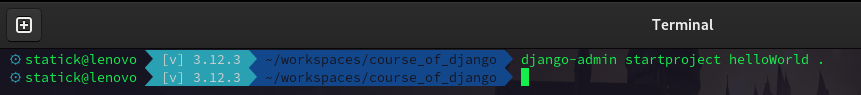
\includegraphics{images/creacion_project_django.png}

}

\caption{Creación de un Proyecto en Django}

\end{figure}%

\begin{Shaded}
\begin{Highlighting}[]
\ExtensionTok{django{-}admin}\NormalTok{ startproject helloWorld .}
\end{Highlighting}
\end{Shaded}

El comando anterior creará un nuevo directorio llamado
\textbf{helloWorld} en el directorio actual, que contendrá un proyecto
de Django.

\section{5. Crear una aplicación de
Django}\label{crear-una-aplicaciuxf3n-de-django}

\begin{figure}[H]

{\centering \includegraphics{images/creacion_app_django.png}

}

\caption{Creación de una App en Django}

\end{figure}%

\begin{Shaded}
\begin{Highlighting}[]
\ExtensionTok{python}\NormalTok{ manage.py startapp hello}
\end{Highlighting}
\end{Shaded}

El comando anterior creará un nuevo directorio llamado \textbf{hello} en
el directorio actual, que contendrá una aplicación de Django.

\begin{tcolorbox}[enhanced jigsaw, breakable, titlerule=0mm, colframe=quarto-callout-tip-color-frame, left=2mm, opacityback=0, rightrule=.15mm, colback=white, opacitybacktitle=0.6, title=\textcolor{quarto-callout-tip-color}{\faLightbulb}\hspace{0.5em}{Tip}, toprule=.15mm, bottomtitle=1mm, leftrule=.75mm, colbacktitle=quarto-callout-tip-color!10!white, toptitle=1mm, coltitle=black, arc=.35mm, bottomrule=.15mm]

Recerda que puedes abrir el editor de código Visual Studio Code con el
comando \textbf{code .}

\end{tcolorbox}

\section{6. Crear una vista}\label{crear-una-vista}

\begin{figure}[H]

{\centering \includegraphics{images/views_hello.png}

}

\caption{Vistas en Django}

\end{figure}%

\begin{Shaded}
\begin{Highlighting}[]
\CommentTok{\# hello/views.py}

\ImportTok{from}\NormalTok{ django.http }\ImportTok{import}\NormalTok{ HttpResponse}

\KeywordTok{def}\NormalTok{ index(request):}
    \ControlFlowTok{return}\NormalTok{ HttpResponse(}\StringTok{"Hello, World!"}\NormalTok{)}
\end{Highlighting}
\end{Shaded}

\section{7. Configurar las URL}\label{configurar-las-url}

\begin{figure}[H]

{\centering \includegraphics{images/urls_app_django.png}

}

\caption{URLs de la App en Django}

\end{figure}%

\begin{Shaded}
\begin{Highlighting}[]
\CommentTok{\# helloWorld/urls.py}

\ImportTok{from}\NormalTok{ django.contrib }\ImportTok{import}\NormalTok{ admin}
\ImportTok{from}\NormalTok{ django.urls }\ImportTok{import}\NormalTok{ include, path}

\NormalTok{urlpatterns }\OperatorTok{=}\NormalTok{ [}
\NormalTok{    path(}\StringTok{""}\NormalTok{, include(}\StringTok{"hello.urls"}\NormalTok{)),}
\NormalTok{    path(}\StringTok{"admin/"}\NormalTok{, admin.site.urls),}
\NormalTok{]}
\end{Highlighting}
\end{Shaded}

\section{8. Ejecutar el servidor de
desarrollo}\label{ejecutar-el-servidor-de-desarrollo}

\begin{figure}[H]

{\centering \includegraphics{images/servidor_desarrollo_django.png}

}

\caption{Servidor de Desarrollo en Django}

\end{figure}%

\begin{Shaded}
\begin{Highlighting}[]
\ExtensionTok{python}\NormalTok{ manage.py runserver}
\end{Highlighting}
\end{Shaded}

El comando anterior ejecutará el servidor de desarrollo de Django. Para
acceder al servidor, abra un navegador web y vaya a la dirección
\textbf{\url{http://0.0.0.0:8000/}}.

\begin{figure}[H]

{\centering \includegraphics{images/navegador_django.png}

}

\caption{Visualizar el servidor corriendo desde el navegador}

\end{figure}%

\begin{tcolorbox}[enhanced jigsaw, breakable, titlerule=0mm, colframe=quarto-callout-tip-color-frame, left=2mm, opacityback=0, rightrule=.15mm, colback=white, opacitybacktitle=0.6, title=\textcolor{quarto-callout-tip-color}{\faLightbulb}\hspace{0.5em}{Tip}, toprule=.15mm, bottomtitle=1mm, leftrule=.75mm, colbacktitle=quarto-callout-tip-color!10!white, toptitle=1mm, coltitle=black, arc=.35mm, bottomrule=.15mm]

Para detener el servidor de desarrollo, presione \textbf{Ctrl + C} en la
terminal.

\end{tcolorbox}

\section{9. Crear una migración}\label{crear-una-migraciuxf3n}

\begin{figure}[H]

{\centering \includegraphics{images/preparacion_migraciones_django.png}

}

\caption{Preparación de las Migraciones en Django}

\end{figure}%

\begin{Shaded}
\begin{Highlighting}[]
\ExtensionTok{python}\NormalTok{ manage.py makemigrations}
\end{Highlighting}
\end{Shaded}

El comando anterior creará una migración para los cambios en los modelos
de la base de datos.

\section{10. Aplicar una migración}\label{aplicar-una-migraciuxf3n}

\begin{figure}[H]

{\centering \includegraphics{images/migraciones_django.png}

}

\caption{Preparación de las Migraciones en Django}

\end{figure}%

\begin{Shaded}
\begin{Highlighting}[]
\ExtensionTok{python}\NormalTok{ manage.py migrate}
\end{Highlighting}
\end{Shaded}

El comando anterior aplicará la migración a la base de datos.

\section{12. Crear un superusuario}\label{crear-un-superusuario}

\begin{figure}[H]

{\centering \includegraphics{images/creacion_superusuario_django.png}

}

\caption{Creación de un Superusuario en Django}

\end{figure}%

\begin{Shaded}
\begin{Highlighting}[]
\ExtensionTok{python}\NormalTok{ manage.py createsuperuser}
\end{Highlighting}
\end{Shaded}

El comando anterior creará un superusuario para acceder al panel de
administración de Django.

\section{13. Acceder al panel de
administración}\label{acceder-al-panel-de-administraciuxf3n}

\begin{figure}[H]

{\centering \includegraphics{images/login_admin_django.png}

}

\caption{Login Admin en Django}

\end{figure}%

Para acceder al panel de administración de Django, abra un navegador web
y vaya a la dirección \textbf{\url{http://127.0.0.1:8000/admin/}}.
Inicie sesión con el superusuario creado en el paso anterior.

\begin{figure}[H]

{\centering \includegraphics{images/admin_django.png}

}

\caption{Admin en Django}

\end{figure}%

\chapter{Ejercicio}\label{ejercicio-1}

Crear un proyecto de Django llamado \textbf{helloWorld} con una
aplicación llamada \textbf{hello} que muestre un mensaje de bienvenida
en la página de inicio.

Ver solución

\phantomsection\label{annotated-cell-139}%
\begin{Shaded}
\begin{Highlighting}[]
\ExtensionTok{python3} \AttributeTok{{-}m}\NormalTok{ venv env }\hspace*{\fill}\NormalTok{\circled{1}}
\BuiltInTok{source}\NormalTok{ env/bin/activate }\hspace*{\fill}\NormalTok{\circled{2}}
\ExtensionTok{pip}\NormalTok{ install django==4.2 }\hspace*{\fill}\NormalTok{\circled{3}}
\ExtensionTok{django{-}admin}\NormalTok{ startproject helloWorld . }\hspace*{\fill}\NormalTok{\circled{4}}
\ExtensionTok{python}\NormalTok{ manage.py startapp hello }\hspace*{\fill}\NormalTok{\circled{5}}
\end{Highlighting}
\end{Shaded}

\begin{description}
\tightlist
\item[\circled{1}]
Crear un entorno virtual.
\item[\circled{2}]
Activar el entorno virtual.
\item[\circled{3}]
Instalar Django.
\item[\circled{4}]
Crear un proyecto de Django.
\item[\circled{5}]
Crear una aplicación de Django.
\end{description}

\phantomsection\label{annotated-cell-140}%
\begin{Shaded}
\begin{Highlighting}[]
\CommentTok{\# hello/views.py}

\ImportTok{from}\NormalTok{ django.http }\ImportTok{import}\NormalTok{ HttpResponse }\hspace*{\fill}\NormalTok{\circled{1}}

\KeywordTok{def}\NormalTok{ index(request): }\hspace*{\fill}\NormalTok{\circled{2}}
    \ControlFlowTok{return}\NormalTok{ HttpResponse(}\StringTok{"Hello, World!"}\NormalTok{) }\hspace*{\fill}\NormalTok{\circled{3}}
\end{Highlighting}
\end{Shaded}

\begin{description}
\tightlist
\item[\circled{1}]
Importar la clase \textbf{HttpResponse} de \textbf{django.http}.
\item[\circled{2}]
Crear una vista llamada \textbf{index}.
\item[\circled{3}]
Devolver un mensaje de bienvenida.
\end{description}

\phantomsection\label{annotated-cell-141}%
\begin{Shaded}
\begin{Highlighting}[]
\CommentTok{\# helloWorld/urls.py}

\ImportTok{from}\NormalTok{ django.urls }\ImportTok{import}\NormalTok{ path }\hspace*{\fill}\NormalTok{\circled{1}}
\ImportTok{from}\NormalTok{ hello }\ImportTok{import}\NormalTok{ views }\hspace*{\fill}\NormalTok{\circled{2}}

\NormalTok{urlpatterns }\OperatorTok{=}\NormalTok{ [ }\hspace*{\fill}\NormalTok{\circled{3}}
\NormalTok{    path(}\StringTok{""}\NormalTok{, views.index), }\hspace*{\fill}\NormalTok{\circled{4}}
\NormalTok{]}
\end{Highlighting}
\end{Shaded}

\begin{description}
\tightlist
\item[\circled{1}]
Importar la función \textbf{path} de \textbf{django.urls}.
\item[\circled{2}]
Importar el módulo \textbf{views} de la aplicación \textbf{hello}.
\item[\circled{3}]
Crear una lista de rutas.
\item[\circled{4}]
Asociar la ruta raíz con la vista \textbf{index}.
\end{description}

\phantomsection\label{annotated-cell-142}%
\begin{Shaded}
\begin{Highlighting}[]
\CommentTok{\# helloWorld/urls.py}

\ImportTok{from}\NormalTok{ django.contrib }\ImportTok{import}\NormalTok{ admin }\hspace*{\fill}\NormalTok{\circled{1}}
\ImportTok{from}\NormalTok{ django.urls }\ImportTok{import}\NormalTok{ include, path }\hspace*{\fill}\NormalTok{\circled{2}}

\NormalTok{urlpatterns }\OperatorTok{=}\NormalTok{ [ }\hspace*{\fill}\NormalTok{\circled{3}}
\NormalTok{    path(}\StringTok{""}\NormalTok{, include(}\StringTok{"hello.urls"}\NormalTok{)), }\hspace*{\fill}\NormalTok{\circled{4}}
\NormalTok{    path(}\StringTok{"admin/"}\NormalTok{, admin.site.urls), }\hspace*{\fill}\NormalTok{\circled{5}}
\NormalTok{]}
\end{Highlighting}
\end{Shaded}

\begin{description}
\tightlist
\item[\circled{1}]
Importar el módulo \textbf{admin} de \textbf{django.contrib}.
\item[\circled{2}]
Importar la función \textbf{include} y la clase \textbf{path} de
\textbf{django.urls}.
\item[\circled{3}]
Crear una lista de rutas.
\item[\circled{4}]
Incluir las rutas de la aplicación \textbf{hello}.
\item[\circled{5}]
Incluir las rutas del panel de administración.
\end{description}

\phantomsection\label{annotated-cell-143}%
\begin{Shaded}
\begin{Highlighting}[]
\ExtensionTok{python}\NormalTok{ manage.py runserver }\hspace*{\fill}\NormalTok{\circled{1}}
\end{Highlighting}
\end{Shaded}

\begin{description}
\tightlist
\item[\circled{1}]
Ejecutar el servidor de desarrollo.
\end{description}

\chapter{Asignación}\label{asignaciuxf3n-6}

Desarrolla una aplicación web que muestre una lista de productos en la
página de inicio. Cada producto debe tener un nombre, una descripción y
un precio. Además, la aplicación debe tener un panel de administración
donde se puedan agregar, editar y eliminar productos.

\chapter{Estructura de archivos y
carpetas}\label{estructura-de-archivos-y-carpetas}

Django tiene una estructura de archivos y carpetas que se debe seguir
para que el proyecto funcione correctamente. A continuación se muestra
la estructura de archivos y carpetas de un proyecto Django:

\begin{tcolorbox}[enhanced jigsaw, breakable, titlerule=0mm, colframe=quarto-callout-tip-color-frame, left=2mm, opacityback=0, rightrule=.15mm, colback=white, opacitybacktitle=0.6, title=\textcolor{quarto-callout-tip-color}{\faLightbulb}\hspace{0.5em}{Tip}, toprule=.15mm, bottomtitle=1mm, leftrule=.75mm, colbacktitle=quarto-callout-tip-color!10!white, toptitle=1mm, coltitle=black, arc=.35mm, bottomrule=.15mm]

Recuerda crear el entorno virtual y activarlo antes de ejecutar el
comando.

\begin{Shaded}
\begin{Highlighting}[]
\ExtensionTok{python} \AttributeTok{{-}m}\NormalTok{ venv venv}
\BuiltInTok{source}\NormalTok{ venv/bin/activate}
\end{Highlighting}
\end{Shaded}

Creamos un directorio con el siguiente comando:

\begin{Shaded}
\begin{Highlighting}[]
\FunctionTok{mkdir}\NormalTok{ myproject}
\BuiltInTok{cd}\NormalTok{ myproject}
\end{Highlighting}
\end{Shaded}

Instalamos Django con el siguiente comando:

\begin{Shaded}
\begin{Highlighting}[]
\ExtensionTok{pip}\NormalTok{ install django==4.2.0}
\end{Highlighting}
\end{Shaded}

Creamos el proyecto con el siguiente comando:

\begin{Shaded}
\begin{Highlighting}[]
\ExtensionTok{django{-}admin}\NormalTok{ startproject myproject .}
\end{Highlighting}
\end{Shaded}

\end{tcolorbox}

\phantomsection\label{annotated-cell-144}%
\begin{Shaded}
\begin{Highlighting}[]
\NormalTok{├── manage.py \# \textless{}1\textgreater{}}
\NormalTok{└── myproject \# \textless{}2\textgreater{}}
\NormalTok{    ├── asgi.py \# \textless{}3\textgreater{}}
\NormalTok{    ├── \_\_init\_\_.py \# \textless{}4\textgreater{}}
\NormalTok{    ├── settings.py \# \textless{}5\textgreater{}}
\NormalTok{    ├── urls.py \# \textless{}6\textgreater{}}
\NormalTok{    └── wsgi.py \# \textless{}7\textgreater{}}
\end{Highlighting}
\end{Shaded}

1.- Archivo de gestión del proyecto.

2.- Carpeta del proyecto.

3.- Archivo de configuración de ASGI.

4.- Archivo de inicialización del proyecto.

5.- Archivo de configuración del proyecto.

6.- Archivo de configuración de las rutas del proyecto.

7.- Archivo de configuración de WSGI.

\chapter{Creación de una aplicación
Django}\label{creaciuxf3n-de-una-aplicaciuxf3n-django}

Para crear una aplicación Django se debe ejecutar el siguiente comando:

\phantomsection\label{annotated-cell-145}%
\begin{Shaded}
\begin{Highlighting}[]
\ExtensionTok{python}\NormalTok{ manage.py startapp myapp }\hspace*{\fill}\NormalTok{\circled{1}}
\end{Highlighting}
\end{Shaded}

\begin{description}
\tightlist
\item[\circled{1}]
Nombre de la aplicación.
\end{description}

\chapter{Configuración de la base de
datos}\label{configuraciuxf3n-de-la-base-de-datos}

Para configurar la base de datos se debe modificar el archivo
\texttt{settings.py} del proyecto. A continuación se muestra un ejemplo
de configuración de la base de datos:

\phantomsection\label{annotated-cell-146}%
\begin{Shaded}
\begin{Highlighting}[]
\NormalTok{DATABASES }\OperatorTok{=}\NormalTok{ \{}
    \StringTok{\textquotesingle{}default\textquotesingle{}}\NormalTok{: \{}
        \StringTok{\textquotesingle{}ENGINE\textquotesingle{}}\NormalTok{: }\StringTok{\textquotesingle{}django.db.backends.sqlite3\textquotesingle{}}\NormalTok{, }\hspace*{\fill}\NormalTok{\circled{1}}
        \StringTok{\textquotesingle{}NAME\textquotesingle{}}\NormalTok{: BASE\_DIR }\OperatorTok{/} \StringTok{\textquotesingle{}db.sqlite3\textquotesingle{}}\NormalTok{, }\hspace*{\fill}\NormalTok{\circled{2}}
\NormalTok{    \}}
\NormalTok{\}}
\end{Highlighting}
\end{Shaded}

\begin{description}
\tightlist
\item[\circled{1}]
Motor de base de datos.
\item[\circled{2}]
Ruta del archivo de la base de datos.
\end{description}

\textbf{Ejemplo}

En este ejemplo crearemos una aplicación que muestre un mensaje en la
página principal. Para ello, se deben seguir los siguientes pasos:

\begin{enumerate}
\def\labelenumi{\arabic{enumi}.}
\tightlist
\item
  Crear una vista.
\item
  Crear una plantilla.
\item
  Configurar las rutas.
\end{enumerate}

\chapter{Crear una vista}\label{crear-una-vista-1}

Para crear una vista se debe modificar el archivo \textbf{views.py} de
la aplicación. A continuación se muestra un ejemplo de vista:

\begin{Shaded}
\begin{Highlighting}[]
\ImportTok{from}\NormalTok{ django.http }\ImportTok{import}\NormalTok{ HttpResponse}

\KeywordTok{def}\NormalTok{ index(request):}
    \ControlFlowTok{return}\NormalTok{ HttpResponse(}\StringTok{"Hello, world!"}\NormalTok{)}
\end{Highlighting}
\end{Shaded}

\chapter{Crear una plantilla}\label{crear-una-plantilla}

Para crear una plantilla se debe crear una carpeta llamada
\textbf{templates} en la carpeta de la aplicación. A continuación se
muestra un ejemplo de plantilla:

\begin{Shaded}
\begin{Highlighting}[]
\DataTypeTok{\textless{}!DOCTYPE}\NormalTok{ html}\DataTypeTok{\textgreater{}}
\DataTypeTok{\textless{}}\KeywordTok{html}\DataTypeTok{\textgreater{}}
\DataTypeTok{\textless{}}\KeywordTok{head}\DataTypeTok{\textgreater{}}
    \DataTypeTok{\textless{}}\KeywordTok{title}\DataTypeTok{\textgreater{}}\NormalTok{MyApp}\DataTypeTok{\textless{}/}\KeywordTok{title}\DataTypeTok{\textgreater{}}
\DataTypeTok{\textless{}/}\KeywordTok{head}\DataTypeTok{\textgreater{}}
\DataTypeTok{\textless{}}\KeywordTok{body}\DataTypeTok{\textgreater{}}
    \DataTypeTok{\textless{}}\KeywordTok{h1}\DataTypeTok{\textgreater{}}\NormalTok{Hello, world!}\DataTypeTok{\textless{}/}\KeywordTok{h1}\DataTypeTok{\textgreater{}}
\DataTypeTok{\textless{}/}\KeywordTok{body}\DataTypeTok{\textgreater{}}
\DataTypeTok{\textless{}/}\KeywordTok{html}\DataTypeTok{\textgreater{}}
\end{Highlighting}
\end{Shaded}

Para que Django pueda encontrar la plantilla, se debe configurar la ruta
de la plantilla en el archivo \textbf{settings.py} del proyecto. A
continuación se muestra un ejemplo de configuración de la ruta de la
plantilla:

\phantomsection\label{annotated-cell-255}%
\begin{Shaded}
\begin{Highlighting}[]

\NormalTok{TEMPLATES }\OperatorTok{=}\NormalTok{ [}
\NormalTok{    \{}
        \StringTok{\textquotesingle{}BACKEND\textquotesingle{}}\NormalTok{: }\StringTok{\textquotesingle{}django.template.backends.django.DjangoTemplates\textquotesingle{}}\NormalTok{,}
        \StringTok{\textquotesingle{}DIRS\textquotesingle{}}\NormalTok{: [BASE\_DIR }\OperatorTok{/} \StringTok{\textquotesingle{}templates\textquotesingle{}}\NormalTok{], }\hspace*{\fill}\NormalTok{\circled{1}}
        \StringTok{\textquotesingle{}APP\_DIRS\textquotesingle{}}\NormalTok{: }\VariableTok{True}\NormalTok{,}
        \StringTok{\textquotesingle{}OPTIONS\textquotesingle{}}\NormalTok{: \{}
            \StringTok{\textquotesingle{}context\_processors\textquotesingle{}}\NormalTok{: [}
                \StringTok{\textquotesingle{}django.template.context\_processors.debug\textquotesingle{}}\NormalTok{,}
                \StringTok{\textquotesingle{}django.template.context\_processors.request\textquotesingle{}}\NormalTok{,}
                \StringTok{\textquotesingle{}django.contrib.auth.context\_processors.auth\textquotesingle{}}\NormalTok{,}
                \StringTok{\textquotesingle{}django.contrib.messages.context\_processors.messages\textquotesingle{}}\NormalTok{,}
\NormalTok{            ],}
\NormalTok{        \},}
\NormalTok{    \},}
\NormalTok{]}
\end{Highlighting}
\end{Shaded}

\begin{description}
\tightlist
\item[\circled{1}]
Ruta de la plantilla.
\end{description}

\chapter{Configurar las rutas}\label{configurar-las-rutas}

Para configurar las rutas se debe modificar el archivo \textbf{urls.py}
de la aplicación. A continuación se muestra un ejemplo de configuración
de las rutas:

\begin{Shaded}
\begin{Highlighting}[]
\ImportTok{from}\NormalTok{ django.urls }\ImportTok{import}\NormalTok{ path}
\ImportTok{from}\NormalTok{ . }\ImportTok{import}\NormalTok{ views}

\NormalTok{urlpatterns }\OperatorTok{=}\NormalTok{ [}
\NormalTok{    path(}\StringTok{\textquotesingle{}\textquotesingle{}}\NormalTok{, views.index, name}\OperatorTok{=}\StringTok{\textquotesingle{}index\textquotesingle{}}\NormalTok{),}
\NormalTok{]}
\end{Highlighting}
\end{Shaded}

\chapter{Correr el servidor de
desarrollo}\label{correr-el-servidor-de-desarrollo}

Para correr el servidor de desarrollo se debe ejecutar el siguiente
comando:

\begin{Shaded}
\begin{Highlighting}[]
\ExtensionTok{python}\NormalTok{ manage.py runserver}
\end{Highlighting}
\end{Shaded}

\chapter{Acceder a la aplicación}\label{acceder-a-la-aplicaciuxf3n}

Para acceder a la aplicación se debe abrir un navegador web y escribir
la siguiente URL:

\url{http://127.0.0.1:8000/}

Posiblemente sea necesario preparar las migraciones y aplicarlas a la
base de datos:

\phantomsection\label{annotated-cell-151}%
\begin{Shaded}
\begin{Highlighting}[]
\ExtensionTok{python}\NormalTok{ manage.py makemigrations }\hspace*{\fill}\NormalTok{\circled{1}}
\ExtensionTok{python}\NormalTok{ manage.py migrate }\hspace*{\fill}\NormalTok{\circled{2}}
\end{Highlighting}
\end{Shaded}

\begin{description}
\tightlist
\item[\circled{1}]
Prepara las migraciones.
\item[\circled{2}]
Aplica las migraciones a la base de datos.
\end{description}

\chapter{Acceder a la aplicación}\label{acceder-a-la-aplicaciuxf3n-1}

Para acceder a la aplicación se debe abrir un navegador web y escribir
la siguiente URL:

\href{http://127.0.0.1:8000/}{http://127.0.0.0.1:8000/}

Muy bien hecho! Has creado tu primera aplicación Django. Ahora puedes
seguir explorando la documentación oficial de Django para aprender más
sobre el framework.

\chapter{Asignación}\label{asignaciuxf3n-7}

Seguir cada uno de los pasos de esta sección para crear una aplicación
Django que muestre un mensaje en la página principal. La aplicación debe
tener los siguientes archivos y carpetas:

\phantomsection\label{annotated-cell-152}%
\begin{Shaded}
\begin{Highlighting}[]
\NormalTok{├── manage.py \# \textless{}1\textgreater{}}
\NormalTok{├── myproject \# \textless{}2\textgreater{}}
\NormalTok{│   ├── asgi.py \# \textless{}3\textgreater{}}
\NormalTok{│   ├── \_\_init\_\_.py \# \textless{}4\textgreater{}}
\NormalTok{│   ├── settings.py \# \textless{}5\textgreater{}}
\NormalTok{│   ├── urls.py \# \textless{}6\textgreater{}}
\NormalTok{│   └── wsgi.py \# \textless{}7\textgreater{}}
\NormalTok{└── myapp \# \textless{}8\textgreater{}}
\NormalTok{    ├── \_\_init\_\_.py \# \textless{}9\textgreater{}}
\NormalTok{    ├── admin.py \# \textless{}10\textgreater{}}
\NormalTok{    ├── apps.py \# \textless{}11\textgreater{}}
\NormalTok{    ├── migrations \# \textless{}12\textgreater{}}
\NormalTok{    │   └── \_\_init\_\_.py \# \textless{}13\textgreater{}}
\NormalTok{    ├── models.py \# \textless{}14\textgreater{}}
\NormalTok{    ├── tests.py \# \textless{}15\textgreater{}}
\NormalTok{    ├── views.py \# \textless{}16\textgreater{}}
\NormalTok{    └── templates \# \textless{}17\textgreater{}}
\NormalTok{        └── index.html \# \textless{}18\textgreater{}}
\end{Highlighting}
\end{Shaded}

1.- Archivo de gestión del proyecto.

2.- Carpeta del proyecto.

3.- Archivo de configuración de ASGI.

4.- Archivo de inicialización del proyecto.

5.- Archivo de configuración del proyecto.

6.- Archivo de configuración de las rutas del proyecto.

7.- Archivo de configuración de WSGI.

8.- Carpeta de la aplicación.

9.- Archivo de inicialización de la aplicación.

10.- Archivo de configuración del administrador de Django.

11.- Archivo de configuración de la aplicación.

12.- Carpeta de migraciones de la aplicación.

13.- Archivo de inicialización de las migraciones.

14.- Archivo de configuración de los modelos de la aplicación.

15.- Archivo de pruebas de la aplicación.

16.- Archivo de configuración de las vistas de la aplicación.

17.- Carpeta de plantillas de la aplicación.

18.- Archivo de la plantilla de la aplicación.

Recuerda que para que Django pueda encontrar la plantilla, se debe
configurar la ruta de la plantilla en el archivo \textbf{settings.py}
del proyecto. A continuación se muestra un ejemplo de configuración de
la ruta de la plantilla:

\phantomsection\label{annotated-cell-256}%
\begin{Shaded}
\begin{Highlighting}[]

\NormalTok{TEMPLATES }\OperatorTok{=}\NormalTok{ [}
\NormalTok{    \{}
        \StringTok{\textquotesingle{}BACKEND\textquotesingle{}}\NormalTok{: }\StringTok{\textquotesingle{}django.template.backends.django.DjangoTemplates\textquotesingle{}}\NormalTok{,}
        \StringTok{\textquotesingle{}DIRS\textquotesingle{}}\NormalTok{: [BASE\_DIR }\OperatorTok{/} \StringTok{\textquotesingle{}templates\textquotesingle{}}\NormalTok{], }\hspace*{\fill}\NormalTok{\circled{1}}
        \StringTok{\textquotesingle{}APP\_DIRS\textquotesingle{}}\NormalTok{: }\VariableTok{True}\NormalTok{,}
        \StringTok{\textquotesingle{}OPTIONS\textquotesingle{}}\NormalTok{: \{}
            \StringTok{\textquotesingle{}context\_processors\textquotesingle{}}\NormalTok{: [}
                \StringTok{\textquotesingle{}django.template.context\_processors.debug\textquotesingle{}}\NormalTok{,}
                \StringTok{\textquotesingle{}django.template.context\_processors.request\textquotesingle{}}\NormalTok{,}
                \StringTok{\textquotesingle{}django.contrib.auth.context\_processors.auth\textquotesingle{}}\NormalTok{,}
                \StringTok{\textquotesingle{}django.contrib.messages.context\_processors.messages\textquotesingle{}}\NormalTok{,}
\NormalTok{            ],}
\NormalTok{        \},}
\NormalTok{    \},}
\NormalTok{]}
\end{Highlighting}
\end{Shaded}

\begin{description}
\tightlist
\item[\circled{1}]
Ruta de la plantilla.
\end{description}

\chapter{Referencias}\label{referencias}

\begin{itemize}
\tightlist
\item
  \href{https://www.djangoproject}{Django}
\end{itemize}

\chapter{Modelos}\label{modelos}

Para entender este tema crearemos un sistema de gestión de inventario de
productos. Para ello, crearemos una clase \textbf{Producto} que
representará un producto en el inventario. Cada producto tendrá un
nombre, un precio y una cantidad en inventario.

Empezaremos creando un entorno virtual e instalando Django.

\begin{Shaded}
\begin{Highlighting}[]
\ExtensionTok{python} \AttributeTok{{-}m}\NormalTok{ venv env}
\end{Highlighting}
\end{Shaded}

Ahora activaremos el entorno virtual.

\begin{Shaded}
\begin{Highlighting}[]
\BuiltInTok{source}\NormalTok{ env/bin/activate}
\end{Highlighting}
\end{Shaded}

crearemos un directorio llamado \textbf{inventario} y nos moveremos a
ese directorio.

\begin{Shaded}
\begin{Highlighting}[]
\FunctionTok{mkdir}\NormalTok{ inventario}
\end{Highlighting}
\end{Shaded}

\begin{Shaded}
\begin{Highlighting}[]
\BuiltInTok{cd}\NormalTok{ inventario}
\end{Highlighting}
\end{Shaded}

Una vez activado el entorno y creando el directorio \textbf{inventario},
instalaremos Django.

\begin{Shaded}
\begin{Highlighting}[]
\ExtensionTok{pip}\NormalTok{ install django==4.2.0}
\end{Highlighting}
\end{Shaded}

\begin{tcolorbox}[enhanced jigsaw, breakable, titlerule=0mm, colframe=quarto-callout-tip-color-frame, left=2mm, opacityback=0, rightrule=.15mm, colback=white, opacitybacktitle=0.6, title=\textcolor{quarto-callout-tip-color}{\faLightbulb}\hspace{0.5em}{Tip}, toprule=.15mm, bottomtitle=1mm, leftrule=.75mm, colbacktitle=quarto-callout-tip-color!10!white, toptitle=1mm, coltitle=black, arc=.35mm, bottomrule=.15mm]

\textbf{Tip:} Para crear un proyecto de Django, utilizamos el comando
\textbf{django-admin startproject}. En este caso utilizamos la versión
LTS, recuerda que puedes consultar la versión más reciente en la
\href{https://www.djangoproject.com/download/}{página oficial de
Django}. Sin embargo en este caso utilizaremos la versión 4.2.0.

\end{tcolorbox}

Ahora crearemos un \textbf{\emph{proyecto}} de Django llamado
\textbf{inventario}

\begin{Shaded}
\begin{Highlighting}[]
\ExtensionTok{django{-}admin}\NormalTok{ startproject inventario .}
\end{Highlighting}
\end{Shaded}

Luego crearemos una aplicación llamada \textbf{productos}

\begin{Shaded}
\begin{Highlighting}[]
\ExtensionTok{python}\NormalTok{ manage.py startapp productos}
\end{Highlighting}
\end{Shaded}

\textbf{Info:} En Django, un proyecto es un conjunto de aplicaciones web
y un proyecto puede contener múltiples aplicaciones.

Para que la app productos funcione, debemos registrarla en el archivo
\textbf{settings.py} del proyecto \textbf{inventario}.

\begin{Shaded}
\begin{Highlighting}[]
\NormalTok{INSTALLED\_APPS }\OperatorTok{=}\NormalTok{ [}
\NormalTok{    ...}
    \StringTok{"productos"}\NormalTok{,}
\NormalTok{]}
\end{Highlighting}
\end{Shaded}

Ahora crearemos la clase \textbf{Producto} en el archivo
\textbf{models.py} de la aplicación \textbf{productos}.

\begin{Shaded}
\begin{Highlighting}[]
\ImportTok{from}\NormalTok{ django.db }\ImportTok{import}\NormalTok{ models}

\KeywordTok{class}\NormalTok{ Producto(models.Model):}
\NormalTok{    nombre }\OperatorTok{=}\NormalTok{ models.CharField(max\_length}\OperatorTok{=}\DecValTok{100}\NormalTok{)}
\NormalTok{    precio }\OperatorTok{=}\NormalTok{ models.DecimalField(max\_digits}\OperatorTok{=}\DecValTok{10}\NormalTok{, decimal\_places}\OperatorTok{=}\DecValTok{2}\NormalTok{)}
\NormalTok{    cantidad }\OperatorTok{=}\NormalTok{ models.IntegerField()}

    \KeywordTok{def} \FunctionTok{\_\_str\_\_}\NormalTok{(}\VariableTok{self}\NormalTok{):}
        \ControlFlowTok{return} \VariableTok{self}\NormalTok{.nombre}
\end{Highlighting}
\end{Shaded}

\begin{tcolorbox}[enhanced jigsaw, breakable, titlerule=0mm, colframe=quarto-callout-tip-color-frame, left=2mm, opacityback=0, rightrule=.15mm, colback=white, opacitybacktitle=0.6, title=\textcolor{quarto-callout-tip-color}{\faLightbulb}\hspace{0.5em}{Tip}, toprule=.15mm, bottomtitle=1mm, leftrule=.75mm, colbacktitle=quarto-callout-tip-color!10!white, toptitle=1mm, coltitle=black, arc=.35mm, bottomrule=.15mm]

\textbf{Tip:} La función \textbf{\_\_str\_\_} es una función especial
que se llama cuando se convierte un objeto a una cadena de texto.

Los modelos en Django son clases que representan tablas en la base de
datos. Cada atributo de la clase representa una columna en la tabla y
cada instancia de la clase representa una fila en la tabla.

\end{tcolorbox}

\chapter{Registramos la aplicacion en
admin.py}\label{registramos-la-aplicacion-en-admin.py}

Para que Django reconozca la clase \textbf{Producto}, debemos
registrarla en el archivo \textbf{admin.py} de la aplicación
\textbf{productos}.

\phantomsection\label{annotated-cell-266}%
\begin{Shaded}
\begin{Highlighting}[]
\ImportTok{from}\NormalTok{ django.contrib }\ImportTok{import}\NormalTok{ admin}
\ImportTok{from}\NormalTok{ .models }\ImportTok{import}\NormalTok{ Producto }\hspace*{\fill}\NormalTok{\circled{1}}

\NormalTok{admin.site.register(Producto) }\hspace*{\fill}\NormalTok{\circled{2}}
\end{Highlighting}
\end{Shaded}

\begin{description}
\tightlist
\item[\circled{1}]
Importamos la clase \textbf{Producto}.
\item[\circled{2}]
Registramos la clase \textbf{Producto} en el panel de administración de
Django.
\end{description}

\chapter{Vistas en Django}\label{vistas-en-django}

Ahora crearemos las vistas de nuestro sistema en Django. Para ello,
crearemos una función para cada vista que renderizará una plantilla
HTML. Por lo tanto nuestras vistas están basadas en funciones. Sin
embargo tambien existen vistas basadas en clases.

\begin{tcolorbox}[enhanced jigsaw, breakable, titlerule=0mm, colframe=quarto-callout-tip-color-frame, left=2mm, opacityback=0, rightrule=.15mm, colback=white, opacitybacktitle=0.6, title=\textcolor{quarto-callout-tip-color}{\faLightbulb}\hspace{0.5em}{Tip}, toprule=.15mm, bottomtitle=1mm, leftrule=.75mm, colbacktitle=quarto-callout-tip-color!10!white, toptitle=1mm, coltitle=black, arc=.35mm, bottomrule=.15mm]

En Django, una vista es una función que recibe una petición HTTP y
devuelve una respuesta HTTP.

\end{tcolorbox}

\begin{tcolorbox}[enhanced jigsaw, breakable, titlerule=0mm, colframe=quarto-callout-tip-color-frame, left=2mm, opacityback=0, rightrule=.15mm, colback=white, opacitybacktitle=0.6, title=\textcolor{quarto-callout-tip-color}{\faLightbulb}\hspace{0.5em}{Tip}, toprule=.15mm, bottomtitle=1mm, leftrule=.75mm, colbacktitle=quarto-callout-tip-color!10!white, toptitle=1mm, coltitle=black, arc=.35mm, bottomrule=.15mm]

\textbf{¿Qué es un CRUD?}

Un CRUD es un acrónimo que significa \textbf{Crear}, \textbf{Leer},
\textbf{Actualizar} y \textbf{Eliminar}. Es un conjunto de operaciones
básicas que se pueden realizar en una base de datos o en un sistema de
gestión de datos.

\end{tcolorbox}

\section{Listar productos}\label{listar-productos}

Para listar los productos en inventario, crearemos una función
\textbf{listar\_productos} que renderizará la plantilla
\textbf{listar.html} con la lista de productos.

\begin{Shaded}
\begin{Highlighting}[]
\ImportTok{from}\NormalTok{ pyexpat.errors }\ImportTok{import}\NormalTok{ messages}
\ImportTok{from}\NormalTok{ django.shortcuts }\ImportTok{import}\NormalTok{ render, redirect, get\_object\_or\_404}
\ImportTok{from}\NormalTok{ .models }\ImportTok{import}\NormalTok{ Producto}
\ImportTok{from}\NormalTok{ django.urls }\ImportTok{import}\NormalTok{ reverse }

\NormalTok{productos }\OperatorTok{=}\NormalTok{ []}

\KeywordTok{def}\NormalTok{ listar\_productos(request):}
\NormalTok{    productos }\OperatorTok{=}\NormalTok{ Producto.objects.}\BuiltInTok{all}\NormalTok{()}
    \ControlFlowTok{return}\NormalTok{ render(request, }\StringTok{\textquotesingle{}listar.html\textquotesingle{}}\NormalTok{, \{}\StringTok{\textquotesingle{}productos\textquotesingle{}}\NormalTok{: productos\})}
\end{Highlighting}
\end{Shaded}

\section{Agregar producto}\label{agregar-producto}

Para agregar un producto al inventario, crearemos una función
\textbf{agregar\_producto} que recibe los datos del producto a agregar y
lo agrega a la lista de productos.

\begin{Shaded}
\begin{Highlighting}[]
\KeywordTok{def}\NormalTok{ agregar\_producto(request):}
    \ControlFlowTok{if}\NormalTok{ request.method }\OperatorTok{==} \StringTok{"POST"}\NormalTok{:}
\NormalTok{        nombre }\OperatorTok{=}\NormalTok{ request.POST.get(}\StringTok{"nombre"}\NormalTok{)}
\NormalTok{        precio }\OperatorTok{=}\NormalTok{ request.POST.get(}\StringTok{"precio"}\NormalTok{)}
\NormalTok{        cantidad }\OperatorTok{=}\NormalTok{ request.POST.get(}\StringTok{"cantidad"}\NormalTok{)}
\NormalTok{        Producto.objects.create(nombre}\OperatorTok{=}\NormalTok{nombre, precio}\OperatorTok{=}\NormalTok{precio, cantidad}\OperatorTok{=}\NormalTok{cantidad) }
        \ControlFlowTok{return}\NormalTok{ redirect(}\StringTok{\textquotesingle{}productos:listar\_productos\textquotesingle{}}\NormalTok{)}
    \ControlFlowTok{return}\NormalTok{ render(request, }\StringTok{"agregar.html"}\NormalTok{)}
\end{Highlighting}
\end{Shaded}

\section{Actualizar producto}\label{actualizar-producto}

Para actualizar un producto en el inventario, crearemos una función
\textbf{actualizar\_producto} que recibe los datos del producto a
actualizar y actualiza el precio y la cantidad del producto.

\begin{Shaded}
\begin{Highlighting}[]
\KeywordTok{def}\NormalTok{ actualizar\_producto(request, }\BuiltInTok{id}\NormalTok{):}
\NormalTok{    producto }\OperatorTok{=}\NormalTok{ get\_object\_or\_404(Producto, pk}\OperatorTok{=}\BuiltInTok{id}\NormalTok{)}
    \ControlFlowTok{if}\NormalTok{ request.method }\OperatorTok{==} \StringTok{\textquotesingle{}POST\textquotesingle{}}\NormalTok{:}
\NormalTok{        nombre }\OperatorTok{=}\NormalTok{ request.POST.get(}\StringTok{\textquotesingle{}nombre\textquotesingle{}}\NormalTok{)}
\NormalTok{        precio }\OperatorTok{=}\NormalTok{ request.POST.get(}\StringTok{\textquotesingle{}precio\textquotesingle{}}\NormalTok{)}
\NormalTok{        cantidad }\OperatorTok{=}\NormalTok{ request.POST.get(}\StringTok{\textquotesingle{}cantidad\textquotesingle{}}\NormalTok{)}
        
        \CommentTok{\# Actualiza los campos del producto}
\NormalTok{        producto.nombre }\OperatorTok{=}\NormalTok{ nombre}
\NormalTok{        producto.precio }\OperatorTok{=}\NormalTok{ precio}
\NormalTok{        producto.cantidad }\OperatorTok{=}\NormalTok{ cantidad}
\NormalTok{        producto.save()}
        
        \ControlFlowTok{return}\NormalTok{ redirect(}\StringTok{\textquotesingle{}productos:listar\_productos\textquotesingle{}}\NormalTok{)}
    \ControlFlowTok{else}\NormalTok{:}
        \ControlFlowTok{return}\NormalTok{ render(request, }\StringTok{\textquotesingle{}actualizar.html\textquotesingle{}}\NormalTok{, \{}\StringTok{\textquotesingle{}producto\textquotesingle{}}\NormalTok{: producto\})}
\end{Highlighting}
\end{Shaded}

\section{Eliminar producto}\label{eliminar-producto}

Para eliminar un producto del inventario, crearemos una función
\textbf{eliminar\_producto} que recibe el nombre del producto a eliminar
y lo elimina de la lista de productos.

\begin{Shaded}
\begin{Highlighting}[]
\KeywordTok{def}\NormalTok{ eliminar\_producto(request):}
    \ControlFlowTok{if}\NormalTok{ request.method }\OperatorTok{==} \StringTok{"POST"}\NormalTok{:}
\NormalTok{        nombre }\OperatorTok{=}\NormalTok{ request.POST.get(}\StringTok{"nombre"}\NormalTok{)}
        \ControlFlowTok{try}\NormalTok{:}
\NormalTok{            producto }\OperatorTok{=}\NormalTok{ Producto.objects.get(nombre}\OperatorTok{=}\NormalTok{nombre)}
\NormalTok{            producto.delete()}
        \ControlFlowTok{except}\NormalTok{ Producto.DoesNotExist:}
            \ControlFlowTok{pass}
        
        \ControlFlowTok{return}\NormalTok{ redirect(}\StringTok{\textquotesingle{}productos:listar\_productos\textquotesingle{}}\NormalTok{)}
    \ControlFlowTok{return}\NormalTok{ render(request, }\StringTok{"eliminar.html"}\NormalTok{)}
\end{Highlighting}
\end{Shaded}

\section{Buscar producto}\label{buscar-producto}

Para buscar un producto en el inventario, crearemos una función
\textbf{buscar\_producto} que recibe el nombre del producto a buscar y
renderiza la plantilla \textbf{buscar.html} con el producto encontrado.

\begin{Shaded}
\begin{Highlighting}[]
\KeywordTok{def}\NormalTok{ buscar\_producto(request):}
    \ControlFlowTok{if}\NormalTok{ request.method }\OperatorTok{==} \StringTok{"POST"}\NormalTok{:}
\NormalTok{        nombre }\OperatorTok{=}\NormalTok{ request.POST.get(}\StringTok{"nombre"}\NormalTok{)}
        \ControlFlowTok{try}\NormalTok{:}
\NormalTok{            producto }\OperatorTok{=}\NormalTok{ Producto.objects.get(nombre}\OperatorTok{=}\NormalTok{nombre)}
            \ControlFlowTok{return}\NormalTok{ render(request, }\StringTok{"buscar.html"}\NormalTok{, \{}\StringTok{"producto"}\NormalTok{: producto\})}
        \ControlFlowTok{except}\NormalTok{ Producto.DoesNotExist:}
            \ControlFlowTok{return}\NormalTok{ render(request, }\StringTok{"buscar.html"}\NormalTok{, \{}\StringTok{"producto"}\NormalTok{: }\VariableTok{None}\NormalTok{\})}
    \ControlFlowTok{return}\NormalTok{ render(request, }\StringTok{"buscar.html"}\NormalTok{)}
\end{Highlighting}
\end{Shaded}

\chapter{Templates}\label{templates}

Django utiliza un sistema de herencia de plantillas llamado Jinja2.
Adicional a ello uilizaremos un framework de CSS llamado Bootstrap.

\begin{tcolorbox}[enhanced jigsaw, breakable, titlerule=0mm, colframe=quarto-callout-tip-color-frame, left=2mm, opacityback=0, rightrule=.15mm, colback=white, opacitybacktitle=0.6, title=\textcolor{quarto-callout-tip-color}{\faLightbulb}\hspace{0.5em}{Tip}, toprule=.15mm, bottomtitle=1mm, leftrule=.75mm, colbacktitle=quarto-callout-tip-color!10!white, toptitle=1mm, coltitle=black, arc=.35mm, bottomrule=.15mm]

\textbf{Jinja2} es un motor de plantillas para Python que se utiliza en
Django para renderizar plantillas HTML.

\end{tcolorbox}

\begin{tcolorbox}[enhanced jigsaw, breakable, titlerule=0mm, colframe=quarto-callout-tip-color-frame, left=2mm, opacityback=0, rightrule=.15mm, colback=white, opacitybacktitle=0.6, title=\textcolor{quarto-callout-tip-color}{\faLightbulb}\hspace{0.5em}{Tip}, toprule=.15mm, bottomtitle=1mm, leftrule=.75mm, colbacktitle=quarto-callout-tip-color!10!white, toptitle=1mm, coltitle=black, arc=.35mm, bottomrule=.15mm]

\textbf{Bootstrap} es un framework de CSS que se utiliza para crear
sitios web y aplicaciones web responsivos y móviles.

\end{tcolorbox}

Para crear las plantillas de nuestro sistema, crearemos una carpeta
llamada \textbf{templates} en el directorio de la aplicación
\textbf{productos}.

Teniendo la siguiente estructura:

\begin{Shaded}
\begin{Highlighting}[]
\NormalTok{productos/}
\NormalTok{    migrations/}
\NormalTok{    templates/}
\NormalTok{        productos/}
\NormalTok{            base.html}
\NormalTok{            listar.html}
\NormalTok{            agregar.html}
\NormalTok{            actualizar.html}
\NormalTok{            eliminar.html}
\NormalTok{            buscar.html}
\NormalTok{    \_\_init\_\_.py}
\NormalTok{    admin.py}
\NormalTok{    apps.py}
\NormalTok{    models.py}
\NormalTok{    tests.py}
\NormalTok{    views.py}
\end{Highlighting}
\end{Shaded}

\section{Base}\label{base}

Crearemos un archivo \textbf{base.html} que contendrá la estructura base
de todas las páginas de nuestro sistema.

\begin{Shaded}
\begin{Highlighting}[]
\DataTypeTok{\textless{}!DOCTYPE}\NormalTok{ html}\DataTypeTok{\textgreater{}}
\DataTypeTok{\textless{}}\KeywordTok{html}\OtherTok{ lang}\OperatorTok{=}\StringTok{"es"}\DataTypeTok{\textgreater{}}
\DataTypeTok{\textless{}}\KeywordTok{head}\DataTypeTok{\textgreater{}}
    \DataTypeTok{\textless{}}\KeywordTok{meta}\OtherTok{ charset}\OperatorTok{=}\StringTok{"UTF{-}8"}\DataTypeTok{\textgreater{}}
    \DataTypeTok{\textless{}}\KeywordTok{meta}\OtherTok{ name}\OperatorTok{=}\StringTok{"viewport"}\OtherTok{ content}\OperatorTok{=}\StringTok{"width=device{-}width, initial{-}scale=1.0"}\DataTypeTok{\textgreater{}}
    \DataTypeTok{\textless{}}\KeywordTok{title}\DataTypeTok{\textgreater{}}
\NormalTok{        \{\% block title \%\}}
\NormalTok{        Inventario}
\NormalTok{        \{\% endblock \%\}}
    \DataTypeTok{\textless{}/}\KeywordTok{title}\DataTypeTok{\textgreater{}}
    \DataTypeTok{\textless{}}\KeywordTok{link}\OtherTok{ href}\OperatorTok{=}\StringTok{"https://cdn.jsdelivr.net/npm/bootstrap@5.3.3/dist/css/bootstrap.min.css"}\OtherTok{ rel}\OperatorTok{=}\StringTok{"stylesheet"}\OtherTok{ integrity}\OperatorTok{=}\StringTok{"sha384{-}QWTKZyjpPEjISv5WaRU9OFeRpok6YctnYmDr5pNlyT2bRjXh0JMhjY6hW+ALEwIH"}\OtherTok{ crossorigin}\OperatorTok{=}\StringTok{"anonymous"}\DataTypeTok{\textgreater{}}
\DataTypeTok{\textless{}/}\KeywordTok{head}\DataTypeTok{\textgreater{}}
\DataTypeTok{\textless{}}\KeywordTok{body}\DataTypeTok{\textgreater{}}
    \DataTypeTok{\textless{}}\KeywordTok{div}\OtherTok{ class}\OperatorTok{=}\StringTok{"container"}\DataTypeTok{\textgreater{}}
\NormalTok{        \{\% block content \%\} }
\NormalTok{        \{\% endblock \%\}}
    \DataTypeTok{\textless{}/}\KeywordTok{div}\DataTypeTok{\textgreater{}}
\DataTypeTok{\textless{}}\KeywordTok{script}\OtherTok{ src}\OperatorTok{=}\StringTok{"https://cdn.jsdelivr.net/npm/bootstrap@5.3.3/dist/js/bootstrap.bundle.min.js"}\OtherTok{ integrity}\OperatorTok{=}\StringTok{"sha384{-}YvpcrYf0tY3lHB60NNkmXc5s9fDVZLESaAA55NDzOxhy9GkcIdslK1eN7N6jIeHz"}\OtherTok{ crossorigin}\OperatorTok{=}\StringTok{"anonymous"}\DataTypeTok{\textgreater{}\textless{}/}\KeywordTok{script}\DataTypeTok{\textgreater{}}
\DataTypeTok{\textless{}/}\KeywordTok{body}\DataTypeTok{\textgreater{}}
\DataTypeTok{\textless{}/}\KeywordTok{html}\DataTypeTok{\textgreater{}}
\end{Highlighting}
\end{Shaded}

\section{Listar}\label{listar}

Crearemos un archivo \textbf{listar.html} que contendrá la lista de
productos en inventario.

\begin{Shaded}
\begin{Highlighting}[]
\NormalTok{\{\% extends "base.html" \%\}}

\NormalTok{\{\% block title \%\} Listar Productos \{\% endblock \%\}}

\NormalTok{\{\% block content\%\}}
\DataTypeTok{\textless{}}\KeywordTok{h1}\DataTypeTok{\textgreater{}}\NormalTok{Listar Productos}\DataTypeTok{\textless{}/}\KeywordTok{h1}\DataTypeTok{\textgreater{}}
\DataTypeTok{\textless{}}\KeywordTok{ul}\OtherTok{ class}\OperatorTok{=}\StringTok{"list{-}group"}\DataTypeTok{\textgreater{}}
\NormalTok{    \{\% for producto in productos \%\}}
    \DataTypeTok{\textless{}}\KeywordTok{li}\OtherTok{ class}\OperatorTok{=}\StringTok{"list{-}group{-}item"}\DataTypeTok{\textgreater{}} 
\NormalTok{        \{\{ producto.nombre \}\} {-} \{\{ producto.precio \}\} {-} \{\{ producto.cantidad \}\}}
    \DataTypeTok{\textless{}/}\KeywordTok{li}\DataTypeTok{\textgreater{}}
\NormalTok{    \{\% endfor \%\}}
\DataTypeTok{\textless{}/}\KeywordTok{ul}\DataTypeTok{\textgreater{}}
\NormalTok{\{\% endblock\%\}}
\end{Highlighting}
\end{Shaded}

\section{Agregar}\label{agregar}

Crearemos un archivo \textbf{agregar.html} que contendrá un formulario
para agregar un producto al inventario.

\begin{Shaded}
\begin{Highlighting}[]
\NormalTok{\{\% extends "base.html" \%\}}

\NormalTok{\{\% block title \%\}Agregar producto\{\% endblock \%\}}

\NormalTok{\{\% block content \%\}}
\DataTypeTok{\textless{}}\KeywordTok{h1}\DataTypeTok{\textgreater{}}\NormalTok{Agregar producto}\DataTypeTok{\textless{}/}\KeywordTok{h1}\DataTypeTok{\textgreater{}}

\DataTypeTok{\textless{}}\KeywordTok{form}\OtherTok{ action}\OperatorTok{=}\StringTok{"\{\% url \textquotesingle{}productos:agregar\_producto\textquotesingle{} \%\}"}\OtherTok{ method}\OperatorTok{=}\StringTok{"post"}\DataTypeTok{\textgreater{}}
\NormalTok{    \{\% csrf\_token \%\}}
    \DataTypeTok{\textless{}}\KeywordTok{div}\OtherTok{ class}\OperatorTok{=}\StringTok{"mb{-}3"}\DataTypeTok{\textgreater{}}
        \DataTypeTok{\textless{}}\KeywordTok{label}\OtherTok{ for}\OperatorTok{=}\StringTok{"nombre"}\OtherTok{ class}\OperatorTok{=}\StringTok{"form{-}label"}\DataTypeTok{\textgreater{}}\NormalTok{Nombre}\DataTypeTok{\textless{}/}\KeywordTok{label}\DataTypeTok{\textgreater{}}
        \DataTypeTok{\textless{}}\KeywordTok{input}\OtherTok{ type}\OperatorTok{=}\StringTok{"text"}\OtherTok{ class}\OperatorTok{=}\StringTok{"form{-}control"}\OtherTok{ id}\OperatorTok{=}\StringTok{"nombre"}\OtherTok{ name}\OperatorTok{=}\StringTok{"nombre"}\DataTypeTok{\textgreater{}}
    \DataTypeTok{\textless{}/}\KeywordTok{div}\DataTypeTok{\textgreater{}}
    \DataTypeTok{\textless{}}\KeywordTok{div}\OtherTok{ class}\OperatorTok{=}\StringTok{"mb{-}3"}\DataTypeTok{\textgreater{}}
        \DataTypeTok{\textless{}}\KeywordTok{label}\OtherTok{ for}\OperatorTok{=}\StringTok{"precio"}\OtherTok{ class}\OperatorTok{=}\StringTok{"form{-}label"}\DataTypeTok{\textgreater{}}\NormalTok{Precio}\DataTypeTok{\textless{}/}\KeywordTok{label}\DataTypeTok{\textgreater{}}
        \DataTypeTok{\textless{}}\KeywordTok{input}\OtherTok{ type}\OperatorTok{=}\StringTok{"number"}\OtherTok{ class}\OperatorTok{=}\StringTok{"form{-}control"}\OtherTok{ id}\OperatorTok{=}\StringTok{"precio"}\OtherTok{ name}\OperatorTok{=}\StringTok{"precio"}\DataTypeTok{\textgreater{}}
    \DataTypeTok{\textless{}/}\KeywordTok{div}\DataTypeTok{\textgreater{}}
    \DataTypeTok{\textless{}}\KeywordTok{div}\OtherTok{ class}\OperatorTok{=}\StringTok{"mb{-}3"}\DataTypeTok{\textgreater{}}
        \DataTypeTok{\textless{}}\KeywordTok{label}\OtherTok{ for}\OperatorTok{=}\StringTok{"cantidad"}\OtherTok{ class}\OperatorTok{=}\StringTok{"form{-}label"}\DataTypeTok{\textgreater{}}\NormalTok{Cantidad}\DataTypeTok{\textless{}/}\KeywordTok{label}\DataTypeTok{\textgreater{}}
        \DataTypeTok{\textless{}}\KeywordTok{input}\OtherTok{ type}\OperatorTok{=}\StringTok{"number"}\OtherTok{ class}\OperatorTok{=}\StringTok{"form{-}control"}\OtherTok{ id}\OperatorTok{=}\StringTok{"cantidad"}\OtherTok{ name}\OperatorTok{=}\StringTok{"cantidad"}\DataTypeTok{\textgreater{}}
    \DataTypeTok{\textless{}/}\KeywordTok{div}\DataTypeTok{\textgreater{}}
    \DataTypeTok{\textless{}}\KeywordTok{button}\OtherTok{ type}\OperatorTok{=}\StringTok{"submit"}\OtherTok{ class}\OperatorTok{=}\StringTok{"btn btn{-}primary"}\DataTypeTok{\textgreater{}}\NormalTok{Agregar}\DataTypeTok{\textless{}/}\KeywordTok{button}\DataTypeTok{\textgreater{}}
\DataTypeTok{\textless{}/}\KeywordTok{form}\DataTypeTok{\textgreater{}}
\NormalTok{\{\% endblock \%\}}
\end{Highlighting}
\end{Shaded}

\section{Actualizar}\label{actualizar}

Crearemos un archivo \textbf{actualizar.html} que contendrá un
formulario para actualizar un producto en el inventario.

\begin{Shaded}
\begin{Highlighting}[]
\NormalTok{\{\% extends "base.html" \%\}}

\NormalTok{\{\% block title \%\}Actualizar producto\{\% endblock \%\}}

\NormalTok{\{\% block content \%\}}
\DataTypeTok{\textless{}}\KeywordTok{h1}\DataTypeTok{\textgreater{}}\NormalTok{Actualizar producto}\DataTypeTok{\textless{}/}\KeywordTok{h1}\DataTypeTok{\textgreater{}}
\DataTypeTok{\textless{}}\KeywordTok{form}\OtherTok{ action}\OperatorTok{=}\StringTok{"\{\% url \textquotesingle{}productos:actualizar\_producto\textquotesingle{} producto.id \%\}"}\OtherTok{ method}\OperatorTok{=}\StringTok{"post"}\DataTypeTok{\textgreater{}}
\NormalTok{    \{\% csrf\_token \%\}}
    \DataTypeTok{\textless{}}\KeywordTok{input}\OtherTok{ type}\OperatorTok{=}\StringTok{"hidden"}\OtherTok{ name}\OperatorTok{=}\StringTok{"nombre"}\OtherTok{ value}\OperatorTok{=}\StringTok{"\{\{ producto.nombre \}\}"}\DataTypeTok{\textgreater{}}
    \DataTypeTok{\textless{}}\KeywordTok{input}\OtherTok{ type}\OperatorTok{=}\StringTok{"hidden"}\OtherTok{ name}\OperatorTok{=}\StringTok{"id"}\OtherTok{ value}\OperatorTok{=}\StringTok{"\{\{ producto.id \}\}"}\DataTypeTok{\textgreater{}}\NormalTok{ \{\# Agregamos un campo oculto para el ID del producto \#\}}
    \DataTypeTok{\textless{}}\KeywordTok{div}\OtherTok{ class}\OperatorTok{=}\StringTok{"mb{-}3"}\DataTypeTok{\textgreater{}}
        \DataTypeTok{\textless{}}\KeywordTok{label}\OtherTok{ for}\OperatorTok{=}\StringTok{"precio"}\OtherTok{ class}\OperatorTok{=}\StringTok{"form{-}label"}\DataTypeTok{\textgreater{}}\NormalTok{Precio}\DataTypeTok{\textless{}/}\KeywordTok{label}\DataTypeTok{\textgreater{}}
        \DataTypeTok{\textless{}}\KeywordTok{input}\OtherTok{ type}\OperatorTok{=}\StringTok{"number"}\OtherTok{ class}\OperatorTok{=}\StringTok{"form{-}control"}\OtherTok{ id}\OperatorTok{=}\StringTok{"precio"}\OtherTok{ name}\OperatorTok{=}\StringTok{"precio"}\OtherTok{ value}\OperatorTok{=}\StringTok{"\{\{ producto.precio \}\}"}\DataTypeTok{\textgreater{}}
    \DataTypeTok{\textless{}/}\KeywordTok{div}\DataTypeTok{\textgreater{}}
    \DataTypeTok{\textless{}}\KeywordTok{div}\OtherTok{ class}\OperatorTok{=}\StringTok{"mb{-}3"}\DataTypeTok{\textgreater{}}
        \DataTypeTok{\textless{}}\KeywordTok{label}\OtherTok{ for}\OperatorTok{=}\StringTok{"cantidad"}\OtherTok{ class}\OperatorTok{=}\StringTok{"form{-}label"}\DataTypeTok{\textgreater{}}\NormalTok{Cantidad}\DataTypeTok{\textless{}/}\KeywordTok{label}\DataTypeTok{\textgreater{}}
        \DataTypeTok{\textless{}}\KeywordTok{input}\OtherTok{ type}\OperatorTok{=}\StringTok{"number"}\OtherTok{ class}\OperatorTok{=}\StringTok{"form{-}control"}\OtherTok{ id}\OperatorTok{=}\StringTok{"cantidad"}\OtherTok{ name}\OperatorTok{=}\StringTok{"cantidad"}\OtherTok{ value}\OperatorTok{=}\StringTok{"\{\{ producto.cantidad \}\}"}\DataTypeTok{\textgreater{}}
    \DataTypeTok{\textless{}/}\KeywordTok{div}\DataTypeTok{\textgreater{}}
    \DataTypeTok{\textless{}}\KeywordTok{button}\OtherTok{ type}\OperatorTok{=}\StringTok{"submit"}\OtherTok{ class}\OperatorTok{=}\StringTok{"btn btn{-}primary"}\DataTypeTok{\textgreater{}}\NormalTok{Actualizar}\DataTypeTok{\textless{}/}\KeywordTok{button}\DataTypeTok{\textgreater{}}
\DataTypeTok{\textless{}/}\KeywordTok{form}\DataTypeTok{\textgreater{}}
\NormalTok{\{\% endblock \%\}}
\end{Highlighting}
\end{Shaded}

\section{Eliminar}\label{eliminar}

Crearemos un archivo \textbf{eliminar.html} que contendrá un formulario
para eliminar un producto del inventario.

\begin{Shaded}
\begin{Highlighting}[]
\NormalTok{\{\% extends "base.html" \%\}}

\NormalTok{\{\% block title \%\}Eliminar producto\{\% endblock \%\}}

\NormalTok{\{\% block content \%\}}
\DataTypeTok{\textless{}}\KeywordTok{h1}\DataTypeTok{\textgreater{}}\NormalTok{Eliminar producto}\DataTypeTok{\textless{}/}\KeywordTok{h1}\DataTypeTok{\textgreater{}}
\DataTypeTok{\textless{}}\KeywordTok{form}\OtherTok{ action}\OperatorTok{=}\StringTok{"\{\% url \textquotesingle{}productos:eliminar\_producto\textquotesingle{} \%\}"}\OtherTok{ method}\OperatorTok{=}\StringTok{"post"}\DataTypeTok{\textgreater{}}
\NormalTok{    \{\% csrf\_token \%\}  }\CommentTok{\textless{}!{-}{-} Agrega el token CSRF aquí {-}{-}\textgreater{}}
    \DataTypeTok{\textless{}}\KeywordTok{div}\OtherTok{ class}\OperatorTok{=}\StringTok{"mb{-}3"}\DataTypeTok{\textgreater{}}
        \DataTypeTok{\textless{}}\KeywordTok{label}\OtherTok{ for}\OperatorTok{=}\StringTok{"nombre"}\OtherTok{ class}\OperatorTok{=}\StringTok{"form{-}label"}\DataTypeTok{\textgreater{}}\NormalTok{Nombre}\DataTypeTok{\textless{}/}\KeywordTok{label}\DataTypeTok{\textgreater{}}
        \DataTypeTok{\textless{}}\KeywordTok{input}\OtherTok{ type}\OperatorTok{=}\StringTok{"text"}\OtherTok{ class}\OperatorTok{=}\StringTok{"form{-}control"}\OtherTok{ id}\OperatorTok{=}\StringTok{"nombre"}\OtherTok{ name}\OperatorTok{=}\StringTok{"nombre"}\DataTypeTok{\textgreater{}}
    \DataTypeTok{\textless{}/}\KeywordTok{div}\DataTypeTok{\textgreater{}}
    \DataTypeTok{\textless{}}\KeywordTok{button}\OtherTok{ type}\OperatorTok{=}\StringTok{"submit"}\OtherTok{ class}\OperatorTok{=}\StringTok{"btn btn{-}primary"}\DataTypeTok{\textgreater{}}\NormalTok{Eliminar}\DataTypeTok{\textless{}/}\KeywordTok{button}\DataTypeTok{\textgreater{}}
\DataTypeTok{\textless{}/}\KeywordTok{form}\DataTypeTok{\textgreater{}}
\NormalTok{\{\% endblock \%\}}
\end{Highlighting}
\end{Shaded}

\section{Buscar}\label{buscar}

Crearemos un archivo \textbf{buscar.html} que contendrá un formulario
para buscar un producto en el inventario.

\begin{Shaded}
\begin{Highlighting}[]
\NormalTok{\{\% extends "base.html" \%\}}

\NormalTok{\{\% block title \%\}Buscar producto\{\% endblock \%\}}

\NormalTok{\{\% block content \%\}}
\DataTypeTok{\textless{}}\KeywordTok{h1}\DataTypeTok{\textgreater{}}\NormalTok{Buscar producto}\DataTypeTok{\textless{}/}\KeywordTok{h1}\DataTypeTok{\textgreater{}}
\DataTypeTok{\textless{}}\KeywordTok{form}\OtherTok{ action}\OperatorTok{=}\StringTok{"\{\% url \textquotesingle{}productos:buscar\_producto\textquotesingle{} \%\}"}\OtherTok{ method}\OperatorTok{=}\StringTok{"post"}\DataTypeTok{\textgreater{}}
\NormalTok{    \{\% csrf\_token \%\}}
    \DataTypeTok{\textless{}}\KeywordTok{div}\OtherTok{ class}\OperatorTok{=}\StringTok{"mb{-}3"}\DataTypeTok{\textgreater{}}
        \DataTypeTok{\textless{}}\KeywordTok{label}\OtherTok{ for}\OperatorTok{=}\StringTok{"nombre"}\OtherTok{ class}\OperatorTok{=}\StringTok{"form{-}label"}\DataTypeTok{\textgreater{}}\NormalTok{Nombre}\DataTypeTok{\textless{}/}\KeywordTok{label}\DataTypeTok{\textgreater{}}
        \DataTypeTok{\textless{}}\KeywordTok{input}\OtherTok{ type}\OperatorTok{=}\StringTok{"text"}\OtherTok{ class}\OperatorTok{=}\StringTok{"form{-}control"}\OtherTok{ id}\OperatorTok{=}\StringTok{"nombre"}\OtherTok{ name}\OperatorTok{=}\StringTok{"nombre"}\DataTypeTok{\textgreater{}}
    \DataTypeTok{\textless{}/}\KeywordTok{div}\DataTypeTok{\textgreater{}}
    \DataTypeTok{\textless{}}\KeywordTok{button}\OtherTok{ type}\OperatorTok{=}\StringTok{"submit"}\OtherTok{ class}\OperatorTok{=}\StringTok{"btn btn{-}primary"}\DataTypeTok{\textgreater{}}\NormalTok{Buscar}\DataTypeTok{\textless{}/}\KeywordTok{button}\DataTypeTok{\textgreater{}}
\DataTypeTok{\textless{}/}\KeywordTok{form}\DataTypeTok{\textgreater{}}

\NormalTok{\{\% if producto \%\}}
\DataTypeTok{\textless{}}\KeywordTok{div}\OtherTok{ class}\OperatorTok{=}\StringTok{"mt{-}3"}\DataTypeTok{\textgreater{}}
    \DataTypeTok{\textless{}}\KeywordTok{h2}\DataTypeTok{\textgreater{}}\NormalTok{Información del producto:}\DataTypeTok{\textless{}/}\KeywordTok{h2}\DataTypeTok{\textgreater{}}
    \DataTypeTok{\textless{}}\KeywordTok{p}\DataTypeTok{\textgreater{}}\NormalTok{Nombre: \{\{ producto.nombre \}\}}\DataTypeTok{\textless{}/}\KeywordTok{p}\DataTypeTok{\textgreater{}}
    \DataTypeTok{\textless{}}\KeywordTok{p}\DataTypeTok{\textgreater{}}\NormalTok{Precio: \{\{ producto.precio \}\}}\DataTypeTok{\textless{}/}\KeywordTok{p}\DataTypeTok{\textgreater{}}
    \DataTypeTok{\textless{}}\KeywordTok{p}\DataTypeTok{\textgreater{}}\NormalTok{Cantidad: \{\{ producto.cantidad \}\}}\DataTypeTok{\textless{}/}\KeywordTok{p}\DataTypeTok{\textgreater{}}
\DataTypeTok{\textless{}/}\KeywordTok{div}\DataTypeTok{\textgreater{}}
\NormalTok{\{\% endif \%\}}
\NormalTok{\{\% endblock \%\}}
\end{Highlighting}
\end{Shaded}

\chapter{URLs}\label{urls}

Para que nuestro sistema funcione, necesitamos definir las URLs que se
utilizarán para acceder a las diferentes vistas.

\section{URLs en la aplicación y el
proyecto}\label{urls-en-la-aplicaciuxf3n-y-el-proyecto}

En el archivo \textbf{urls.py} de la aplicación \textbf{productos}
definiremos las URLs de las vistas de nuestro sistema.

\begin{Shaded}
\begin{Highlighting}[]
\ImportTok{from}\NormalTok{ django.urls }\ImportTok{import}\NormalTok{ path}
\ImportTok{from}\NormalTok{ . }\ImportTok{import}\NormalTok{ views}

\NormalTok{app\_name }\OperatorTok{=} \StringTok{\textquotesingle{}productos\textquotesingle{}}

\NormalTok{urlpatterns }\OperatorTok{=}\NormalTok{ [}
\NormalTok{    path(}\StringTok{\textquotesingle{}\textquotesingle{}}\NormalTok{, views.listar\_productos, name}\OperatorTok{=}\StringTok{\textquotesingle{}listar\_productos\textquotesingle{}}\NormalTok{),}
\NormalTok{    path(}\StringTok{\textquotesingle{}agregar/\textquotesingle{}}\NormalTok{, views.agregar\_producto, name}\OperatorTok{=}\StringTok{\textquotesingle{}agregar\_producto\textquotesingle{}}\NormalTok{),}
\NormalTok{    path(}\StringTok{\textquotesingle{}actualizar/\textless{}int:id\textgreater{}/\textquotesingle{}}\NormalTok{, views.actualizar\_producto, name}\OperatorTok{=}\StringTok{\textquotesingle{}actualizar\_producto\textquotesingle{}}\NormalTok{),}
\NormalTok{    path(}\StringTok{\textquotesingle{}eliminar/\textquotesingle{}}\NormalTok{, views.eliminar\_producto, name}\OperatorTok{=}\StringTok{\textquotesingle{}eliminar\_producto\textquotesingle{}}\NormalTok{),}
\NormalTok{    path(}\StringTok{\textquotesingle{}buscar/\textquotesingle{}}\NormalTok{, views.buscar\_producto, name}\OperatorTok{=}\StringTok{\textquotesingle{}buscar\_producto\textquotesingle{}}\NormalTok{),}
\NormalTok{]}
\end{Highlighting}
\end{Shaded}

En el archivo \textbf{urls.py} del proyecto \textbf{inventario}
incluiremos las URLs de la aplicación \textbf{productos}.

\begin{Shaded}
\begin{Highlighting}[]
\ImportTok{from}\NormalTok{ django.contrib }\ImportTok{import}\NormalTok{ admin}
\ImportTok{from}\NormalTok{ django.urls }\ImportTok{import}\NormalTok{ path, include}

\NormalTok{urlpatterns }\OperatorTok{=}\NormalTok{ [}
\NormalTok{    path(}\StringTok{\textquotesingle{}admin/\textquotesingle{}}\NormalTok{, admin.site.urls),}
\NormalTok{    path(}\StringTok{\textquotesingle{}\textquotesingle{}}\NormalTok{, include(}\StringTok{\textquotesingle{}productos.urls\textquotesingle{}}\NormalTok{)),}
\NormalTok{]}
\end{Highlighting}
\end{Shaded}

\begin{tcolorbox}[enhanced jigsaw, breakable, titlerule=0mm, colframe=quarto-callout-tip-color-frame, left=2mm, opacityback=0, rightrule=.15mm, colback=white, opacitybacktitle=0.6, title=\textcolor{quarto-callout-tip-color}{\faLightbulb}\hspace{0.5em}{Tip}, toprule=.15mm, bottomtitle=1mm, leftrule=.75mm, colbacktitle=quarto-callout-tip-color!10!white, toptitle=1mm, coltitle=black, arc=.35mm, bottomrule=.15mm]

\textbf{Tip:} Para acceder al panel de administración de Django, debemos
crear un superusuario con el siguiente comando.

\begin{Shaded}
\begin{Highlighting}[]
\ExtensionTok{python}\NormalTok{ manage.py createsuperuser}
\end{Highlighting}
\end{Shaded}

\end{tcolorbox}

\begin{tcolorbox}[enhanced jigsaw, breakable, titlerule=0mm, colframe=quarto-callout-tip-color-frame, left=2mm, opacityback=0, rightrule=.15mm, colback=white, opacitybacktitle=0.6, title=\textcolor{quarto-callout-tip-color}{\faLightbulb}\hspace{0.5em}{Tip}, toprule=.15mm, bottomtitle=1mm, leftrule=.75mm, colbacktitle=quarto-callout-tip-color!10!white, toptitle=1mm, coltitle=black, arc=.35mm, bottomrule=.15mm]

Si realizamos modificaciones en el modelo de datos, debemos aplicar las
migraciones con el siguiente comando.

\phantomsection\label{annotated-cell-284}%
\begin{Shaded}
\begin{Highlighting}[]
\ExtensionTok{python}\NormalTok{ manage.py makemigrations }\hspace*{\fill}\NormalTok{\circled{1}}
\ExtensionTok{python}\NormalTok{ manage.py migrate }\hspace*{\fill}\NormalTok{\circled{2}}
\end{Highlighting}
\end{Shaded}

\begin{description}
\tightlist
\item[\circled{1}]
Crea las migraciones.
\item[\circled{2}]
Aplica las migraciones.
\end{description}

\end{tcolorbox}

\begin{tcolorbox}[enhanced jigsaw, breakable, titlerule=0mm, colframe=quarto-callout-tip-color-frame, left=2mm, opacityback=0, rightrule=.15mm, colback=white, opacitybacktitle=0.6, title=\textcolor{quarto-callout-tip-color}{\faLightbulb}\hspace{0.5em}{Tip}, toprule=.15mm, bottomtitle=1mm, leftrule=.75mm, colbacktitle=quarto-callout-tip-color!10!white, toptitle=1mm, coltitle=black, arc=.35mm, bottomrule=.15mm]

\textbf{Tip:} Para acceder a las vistas de nuestro sistema, debemos
definir las URLs en el archivo \textbf{urls.py} de la aplicación y el
proyecto.

En Django, las URLs se definen en el archivo \textbf{urls.py} de la
aplicación y el proyecto. Las URLs se utilizan para acceder a las vistas
de nuestro sistema.

\end{tcolorbox}

Es necesario realizar una modificación en el archivo
\textbf{settings.py} del proyecto \textbf{inventario} para que Django
pueda encontrar las plantillas de nuestro sistema.

\phantomsection\label{annotated-cell-281}%
\begin{Shaded}
\begin{Highlighting}[]
\NormalTok{TEMPLATES }\OperatorTok{=}\NormalTok{ [}
\NormalTok{    \{}
\NormalTok{        ...}
        \StringTok{\textquotesingle{}DIRS\textquotesingle{}}\NormalTok{: [os.path.join(BASE\_DIR, }\StringTok{\textquotesingle{}templates\textquotesingle{}}\NormalTok{)], }\hspace*{\fill}\NormalTok{\circled{1}}
\NormalTok{        ...}
\NormalTok{    \},}
\NormalTok{]}
\end{Highlighting}
\end{Shaded}

\begin{description}
\tightlist
\item[\circled{1}]
Agregamos la ruta de la carpeta \textbf{templates} al directorio de
plantillas.
\end{description}

\chapter{Ejecutar el servidor}\label{ejecutar-el-servidor}

Para ejecutar el servidor de desarrollo de Django, utilizaremos el
siguiente comando.

\begin{Shaded}
\begin{Highlighting}[]
\ExtensionTok{python}\NormalTok{ manage.py runserver}
\end{Highlighting}
\end{Shaded}

Con esto hemos creado un sistema de gestión de inventario de productos
con Django. Ahora podemos listar, agregar, actualizar, eliminar y buscar
productos en el inventario y hemos utilizado el sistema de plantillas de
Django para crear las vistas de nuestro sistema. Adicional a ello
tambien hemos utilizado el framework de CSS Bootstrap para darle estilo
a nuestro sistema.

\chapter{Conclusiones}\label{conclusiones}

En este tema hemos aprendido a crear un sistema de gestión de inventario
de productos con Django. Hemos creado un modelo de datos para
representar los productos en el inventario y hemos creado vistas para
listar, agregar, actualizar, eliminar y buscar productos en el
inventario. Adicional a ello tambien hemos creado plantillas HTML para
renderizar las vistas de nuestro sistema.

\chapter{Django Rest Framework}\label{django-rest-framework}

\textbf{Django Rest Framework} más que una \textbf{librearía} es un
\textbf{framework} que nos permite crear \textbf{APIs REST} de forma
rápida y sencilla.

\section{¿Qué es una API REST?}\label{quuxe9-es-una-api-rest}

Una \textbf{API REST} (Representational State Transfer) es una
\textbf{interfaz de programación de aplicaciones} que utiliza los
métodos HTTP para realizar operaciones CRUD (Crear, Leer, Actualizar,
Eliminar) en recursos.

\section{Instalación}\label{instalaciuxf3n}

Para instalar Django Rest Framework, ejecutamos el siguiente comando:

\begin{Shaded}
\begin{Highlighting}[]
\ExtensionTok{pip}\NormalTok{ install djangorestframework}
\end{Highlighting}
\end{Shaded}

Una vez instalado, añadimos \textbf{`rest\_framework'} a la lista de
aplicaciones instaladas en el archivo settings.py:

\begin{Shaded}
\begin{Highlighting}[]
\NormalTok{INSTALLED\_APPS }\OperatorTok{=}\NormalTok{ [}
\NormalTok{    ...}
    \StringTok{\textquotesingle{}rest\_framework\textquotesingle{}}\NormalTok{,}
\NormalTok{]}
\end{Highlighting}
\end{Shaded}

\section{Actualizar el archivo
requirements.txt}\label{actualizar-el-archivo-requirements.txt}

Es necesario \textbf{eliminar} el archivo \textbf{requirements.txt} y
volver a crearlo con el siguiente comando:

\begin{Shaded}
\begin{Highlighting}[]
\ExtensionTok{pip}\NormalTok{ freeze }\OperatorTok{\textgreater{}}\NormalTok{ requirements.txt}
\end{Highlighting}
\end{Shaded}

\section{Serializers}\label{serializers}

Los serializadores nos permiten convertir los datos de nuestro modelo en
un formato que pueda ser fácilmente consumido por una API REST.

Para crear un serializador, creamos un archivo serializers.py en la
carpeta de nuestra aplicación y añadimos el siguiente código:

\phantomsection\label{annotated-cell-156}%
\begin{Shaded}
\begin{Highlighting}[]
\ImportTok{from}\NormalTok{ rest\_framework }\ImportTok{import}\NormalTok{ serializers }\hspace*{\fill}\NormalTok{\circled{1}}
\ImportTok{from}\NormalTok{ .models }\ImportTok{import}\NormalTok{ Producto}

\KeywordTok{class}\NormalTok{ ProductoSerializer(serializers.ModelSerializer): }\hspace*{\fill}\NormalTok{\circled{2}}
    \KeywordTok{class}\NormalTok{ Meta: }\hspace*{\fill}\NormalTok{\circled{3}}
\NormalTok{        model }\OperatorTok{=}\NormalTok{ Producto }\hspace*{\fill}\NormalTok{\circled{4}}
\NormalTok{        fields }\OperatorTok{=} \StringTok{\textquotesingle{}\_\_all\_\_\textquotesingle{}} \hspace*{\fill}\NormalTok{\circled{5}}
\end{Highlighting}
\end{Shaded}

\begin{description}
\tightlist
\item[\circled{1}]
Importamos el módulo serializers de Django Rest Framework.
\item[\circled{2}]
Creamos un serializador ProductoSerializer que hereda de
serializers.ModelSerializer.
\item[\circled{3}]
Definimos la clase Meta para configurar el serializador.
\item[\circled{4}]
Especificamos el modelo Producto que queremos serializar.
\item[\circled{5}]
Indicamos que queremos serializar todos los campos del modelo Producto.
\end{description}

\section{Views}\label{views}

Las vistas en Django Rest Framework son similares a las vistas en
Django. En lugar de devolver una \textbf{respuesta HTML}, devuelven una
\textbf{respuesta JSON} que puede ser consumida por una \textbf{API
REST}.

Para crear una vista, creamos un archivo \textbf{views.py} en la carpeta
de nuestra aplicación y añadimos el siguiente código:

\phantomsection\label{annotated-cell-157}%
\begin{Shaded}
\begin{Highlighting}[]
\ImportTok{from}\NormalTok{ rest\_framework }\ImportTok{import}\NormalTok{ viewsets }\hspace*{\fill}\NormalTok{\circled{1}}
\ImportTok{from}\NormalTok{ .serializers }\ImportTok{import}\NormalTok{ ProductoSerializer }\hspace*{\fill}\NormalTok{\circled{2}}
\ImportTok{from}\NormalTok{ .models }\ImportTok{import}\NormalTok{ Producto}

\KeywordTok{class}\NormalTok{ ProductoViewSet(viewsets.ModelViewSet): }\hspace*{\fill}\NormalTok{\circled{3}}
\NormalTok{    queryset }\OperatorTok{=}\NormalTok{ Producto.objects.}\BuiltInTok{all}\NormalTok{() }\hspace*{\fill}\NormalTok{\circled{4}}
\NormalTok{    serializer\_class }\OperatorTok{=}\NormalTok{ ProductoSerializer }\hspace*{\fill}\NormalTok{\circled{5}}
\end{Highlighting}
\end{Shaded}

\begin{description}
\tightlist
\item[\circled{1}]
Importamos el módulo viewsets de Django Rest Framework.
\item[\circled{2}]
Importamos el serializador ProductoSerializer que creamos anteriormente.
\item[\circled{3}]
Creamos una vista ProductoViewSet que hereda de viewsets.ModelViewSet.
\end{description}

\section{URLs de la Aplicación}\label{urls-de-la-aplicaciuxf3n}

Para conectar nuestras vistas con las URLs de nuestra aplicación,
creamos un archivo urls.py en la carpeta de nuestra aplicación y
añadimos el siguiente código:

\phantomsection\label{annotated-cell-158}%
\begin{Shaded}
\begin{Highlighting}[]
\ImportTok{from}\NormalTok{ django.urls }\ImportTok{import}\NormalTok{ path}
\ImportTok{from}\NormalTok{ .views }\ImportTok{import}\NormalTok{ ProductoViewSet }\hspace*{\fill}\NormalTok{\circled{1}}

\NormalTok{urlpatterns }\OperatorTok{=}\NormalTok{ [}
\NormalTok{    path(}\StringTok{\textquotesingle{}api/productos/\textquotesingle{}}\NormalTok{, ProductoViewSet.as\_view(\{}\StringTok{\textquotesingle{}get\textquotesingle{}}\NormalTok{: }\StringTok{\textquotesingle{}list\textquotesingle{}}\NormalTok{, }\StringTok{\textquotesingle{}post\textquotesingle{}}\NormalTok{: }\StringTok{\textquotesingle{}create\textquotesingle{}}\NormalTok{\}), name}\OperatorTok{=}\StringTok{\textquotesingle{}api{-}productos\textquotesingle{}}\NormalTok{), }\hspace*{\fill}\NormalTok{\circled{2}}
\NormalTok{    path(}\StringTok{\textquotesingle{}api/productos/\textless{}int:pk\textgreater{}/\textquotesingle{}}\NormalTok{, ProductoViewSet.as\_view(\{}\StringTok{\textquotesingle{}get\textquotesingle{}}\NormalTok{: }\StringTok{\textquotesingle{}retrieve\textquotesingle{}}\NormalTok{, }\StringTok{\textquotesingle{}put\textquotesingle{}}\NormalTok{: }\StringTok{\textquotesingle{}update\textquotesingle{}}\NormalTok{, }\StringTok{\textquotesingle{}delete\textquotesingle{}}\NormalTok{: }\StringTok{\textquotesingle{}destroy\textquotesingle{}}\NormalTok{\}), name}\OperatorTok{=}\StringTok{\textquotesingle{}api{-}producto{-}detail\textquotesingle{}}\NormalTok{), }\hspace*{\fill}\NormalTok{\circled{3}}
\NormalTok{]}
\end{Highlighting}
\end{Shaded}

\begin{description}
\tightlist
\item[\circled{1}]
Importamos la vista ProductoViewSet que creamos anteriormente.
\item[\circled{2}]
Configuramos la URL `/api/productos/' para listar y crear productos.
\item[\circled{3}]
Configuramos la URL `/api/productos/\textless int:pk\textgreater/' para
ver, actualizar y eliminar un producto específico.
\end{description}

\section{Configuración URLs del
Proyecto}\label{configuraciuxf3n-urls-del-proyecto}

Para configurar nuestra API REST, añadimos las URLs de nuestra
aplicación a las URLs del proyecto en el archivo urls.py de la carpeta
del proyecto:

\begin{Shaded}
\begin{Highlighting}[]
\ImportTok{from}\NormalTok{ django.contrib }\ImportTok{import}\NormalTok{ admin}
\ImportTok{from}\NormalTok{ django.urls }\ImportTok{import}\NormalTok{ path, include}
\ImportTok{from}\NormalTok{ rest\_framework }\ImportTok{import}\NormalTok{ routers}
\ImportTok{from}\NormalTok{ productos.views }\ImportTok{import}\NormalTok{ ProductoViewSet}

\CommentTok{\# Creamos un enrutador para las vistas de Django REST Framework}
\NormalTok{router }\OperatorTok{=}\NormalTok{ routers.DefaultRouter()}
\NormalTok{router.register(}\VerbatimStringTok{r\textquotesingle{}productos\textquotesingle{}}\NormalTok{, ProductoViewSet)}

\NormalTok{urlpatterns }\OperatorTok{=}\NormalTok{ [}
\NormalTok{    path(}\StringTok{\textquotesingle{}admin/\textquotesingle{}}\NormalTok{, admin.site.urls),}
\NormalTok{    path(}\StringTok{\textquotesingle{}\textquotesingle{}}\NormalTok{, include(}\StringTok{\textquotesingle{}productos.urls\textquotesingle{}}\NormalTok{)),}
\NormalTok{    path(}\StringTok{\textquotesingle{}api/\textquotesingle{}}\NormalTok{, include(router.urls)),}
\NormalTok{]}
\end{Highlighting}
\end{Shaded}

\section{Migraciones}\label{migraciones}

Antes de utilizar nuestra API REST, debemos aplicar las migraciones
necesarias para crear las tablas en la base de datos:

\begin{Shaded}
\begin{Highlighting}[]
\ExtensionTok{python}\NormalTok{ manage.py makemigrations}
\ExtensionTok{python}\NormalTok{ manage.py migrate}
\end{Highlighting}
\end{Shaded}

\section{Instalación de setuptools}\label{instalaciuxf3n-de-setuptools}

Para instalar setuptools, ejecutamos el siguiente comando:

\begin{Shaded}
\begin{Highlighting}[]
\ExtensionTok{pip}\NormalTok{ install setuptools}
\end{Highlighting}
\end{Shaded}

Es necesario la instalación de setuptools para poder instalar las
dependencias necesarias para el proyecto.

\section{Ejecución}\label{ejecuciuxf3n-1}

Una vez configurada nuestra API REST, podemos ejecutar el servidor de
desarrollo de Django y acceder a la API a través de un navegador o una
herramienta como Postman:

\begin{Shaded}
\begin{Highlighting}[]
\ExtensionTok{python}\NormalTok{ manage.py runserver}
\end{Highlighting}
\end{Shaded}

En este caso, la API estará disponible en la ruta
`http://127.0.0.1:8000/api/productos/'.

\chapter{Documentación de la API con
drf-yasg}\label{documentaciuxf3n-de-la-api-con-drf-yasg}

Primero instalamos el paquete de documentación de la API:

\begin{Shaded}
\begin{Highlighting}[]
\ExtensionTok{pip}\NormalTok{ install drf{-}yasg}
\end{Highlighting}
\end{Shaded}

Luego, añadimos `drf\_yasg' a la lista de aplicaciones instaladas en el
archivo settings.py:

\begin{Shaded}
\begin{Highlighting}[]
\NormalTok{INSTALLED\_APPS }\OperatorTok{=}\NormalTok{ [}
\NormalTok{    ...}
    \StringTok{\textquotesingle{}drf\_yasg\textquotesingle{}}\NormalTok{,}
\NormalTok{]}
\end{Highlighting}
\end{Shaded}

Añadimos las URLs de la documentación de la API a las URLs del proyecto
en el archivo urls.py de la carpeta del proyecto:

\begin{Shaded}
\begin{Highlighting}[]
\ImportTok{from}\NormalTok{ django.urls }\ImportTok{import}\NormalTok{ path, include}
\ImportTok{from}\NormalTok{ rest\_framework }\ImportTok{import}\NormalTok{ routers}
\ImportTok{from}\NormalTok{ productos.views }\ImportTok{import}\NormalTok{ ProductoViewSet}
\ImportTok{from}\NormalTok{ rest\_framework.permissions }\ImportTok{import}\NormalTok{ AllowAny}
\ImportTok{from}\NormalTok{ drf\_yasg.views }\ImportTok{import}\NormalTok{ get\_schema\_view}
\ImportTok{from}\NormalTok{ drf\_yasg }\ImportTok{import}\NormalTok{ openapi}

\NormalTok{router }\OperatorTok{=}\NormalTok{ routers.DefaultRouter()}
\NormalTok{router.register(}\VerbatimStringTok{r\textquotesingle{}productos\textquotesingle{}}\NormalTok{, ProductoViewSet)}

\NormalTok{schema\_view }\OperatorTok{=}\NormalTok{ get\_schema\_view(}
\NormalTok{   openapi.Info(}
\NormalTok{      title}\OperatorTok{=}\StringTok{"API de Productos"}\NormalTok{,}
\NormalTok{      default\_version}\OperatorTok{=}\StringTok{\textquotesingle{}v1\textquotesingle{}}\NormalTok{,}
\NormalTok{      description}\OperatorTok{=}\StringTok{"Documentación de la API de Productos"}\NormalTok{,}
\NormalTok{      terms\_of\_service}\OperatorTok{=}\StringTok{"https://www.google.com/policies/terms/"}\NormalTok{,}
\NormalTok{      contact}\OperatorTok{=}\NormalTok{openapi.Contact(email}\OperatorTok{=}\StringTok{"contact@example.com"}\NormalTok{),}
\NormalTok{      license}\OperatorTok{=}\NormalTok{openapi.License(name}\OperatorTok{=}\StringTok{"BSD License"}\NormalTok{),}
\NormalTok{   ),}
\NormalTok{   public}\OperatorTok{=}\VariableTok{True}\NormalTok{,}
\NormalTok{   permission\_classes}\OperatorTok{=}\NormalTok{(AllowAny,),}
\NormalTok{)}

\NormalTok{urlpatterns }\OperatorTok{=}\NormalTok{ [}
\NormalTok{    path(}\StringTok{\textquotesingle{}admin/\textquotesingle{}}\NormalTok{, admin.site.urls),}
\NormalTok{    path(}\StringTok{\textquotesingle{}\textquotesingle{}}\NormalTok{, include(}\StringTok{\textquotesingle{}productos.urls\textquotesingle{}}\NormalTok{)),}
\NormalTok{    path(}\StringTok{\textquotesingle{}api/\textquotesingle{}}\NormalTok{, include(router.urls)),}
\NormalTok{    path(}\StringTok{\textquotesingle{}swagger/\textquotesingle{}}\NormalTok{, schema\_view.with\_ui(}\StringTok{\textquotesingle{}swagger\textquotesingle{}}\NormalTok{, cache\_timeout}\OperatorTok{=}\DecValTok{0}\NormalTok{), name}\OperatorTok{=}\StringTok{\textquotesingle{}schema{-}swagger{-}ui\textquotesingle{}}\NormalTok{),}
\NormalTok{    path(}\StringTok{\textquotesingle{}redoc/\textquotesingle{}}\NormalTok{, schema\_view.with\_ui(}\StringTok{\textquotesingle{}redoc\textquotesingle{}}\NormalTok{, cache\_timeout}\OperatorTok{=}\DecValTok{0}\NormalTok{), name}\OperatorTok{=}\StringTok{\textquotesingle{}schema{-}redoc\textquotesingle{}}\NormalTok{),}
\NormalTok{]}
\end{Highlighting}
\end{Shaded}

Una vez configurada la documentación de la API, podemos ejecutar el
servidor de desarrollo de Django y acceder a la documentación de la API
a través de un navegador:

\begin{Shaded}
\begin{Highlighting}[]
\ExtensionTok{python}\NormalTok{ manage.py runserver}
\end{Highlighting}
\end{Shaded}

\chapter{Documentación de la API con
CoreAPI}\label{documentaciuxf3n-de-la-api-con-coreapi}

CoreAPI es una biblioteca que facilita la creación y el consumo de APIs.

\section{Primero instalamos CoreAPI:}\label{primero-instalamos-coreapi}

\begin{Shaded}
\begin{Highlighting}[]
\ExtensionTok{pip}\NormalTok{ install coreapi}
\end{Highlighting}
\end{Shaded}

Para generar la documentación automáticamente, agregamos la
configuración en settings.py:

\begin{Shaded}
\begin{Highlighting}[]
\NormalTok{REST\_FRAMEWORK }\OperatorTok{=}\NormalTok{ \{}
    \StringTok{\textquotesingle{}DEFAULT\_SCHEMA\_CLASS\textquotesingle{}}\NormalTok{: }\StringTok{\textquotesingle{}rest\_framework.schemas.coreapi.AutoSchema\textquotesingle{}}
\NormalTok{\}}
\end{Highlighting}
\end{Shaded}

Luego, añadimos la vista de esquema en el archivo urls.py de la carpeta
del proyecto:

\begin{Shaded}
\begin{Highlighting}[]
\ImportTok{from}\NormalTok{ rest\_framework.schemas }\ImportTok{import}\NormalTok{ get\_schema\_view}

\NormalTok{schema\_view }\OperatorTok{=}\NormalTok{ get\_schema\_view(title}\OperatorTok{=}\StringTok{\textquotesingle{}API de Productos\textquotesingle{}}\NormalTok{)}

\NormalTok{urlpatterns }\OperatorTok{+=}\NormalTok{ [}
\NormalTok{    path(}\StringTok{\textquotesingle{}docs/\textquotesingle{}}\NormalTok{, schema\_view, name}\OperatorTok{=}\StringTok{\textquotesingle{}api{-}docs\textquotesingle{}}\NormalTok{),}
\NormalTok{]}
\end{Highlighting}
\end{Shaded}

Ahora podemos ejecutar el servidor de desarrollo y acceder a la
documentación generada por CoreAPI en la ruta `/docs/':

\begin{Shaded}
\begin{Highlighting}[]
\ExtensionTok{python}\NormalTok{ manage.py runserver}
\end{Highlighting}
\end{Shaded}

Con estos pasos, hemos integrado Django Rest Framework, documentado
nuestra API con drf-yasg y CoreAPI.

\chapter{Bases de Dato en Django}\label{bases-de-dato-en-django}

\includegraphics{unidades/unidad5/images/paste-1.png}

En este capítulo, aprenderemos a trabajar con bases de datos en Django.
Crearemos un modelo de base de datos para almacenar información sobre
productos y luego lo expondremos a través de una API REST.

Utilizaremos tanto bases de datos relacionales como no relacionales para
almacenar información sobre productos. Crearemos un modelo de base de
datos para almacenar información sobre productos y luego lo expondremos
a través de una API REST.

Utilizaremos un entorno docker para ejecutar una base de datos
PostgreSQL y otra base de datos MongoDB. Luego, configuraremos Django
para conectarse a estas bases de datos y almacenar información sobre
productos.

Para ello iniciaremos un nuevo proyecto donde crearemos un sistema que
permita administrar una biblioteca de libros. Crearemos dos modelos de
base de datos: uno para almacenar información sobre los libros y otro
para almacenar información sobre los autores.

\section{Objetivos}\label{objetivos-1}

\begin{itemize}
\item
  \textbf{Modelos de Base de Datos:} Crear modelos de base de datos para
  almacenar información sobre libros y autores.
\item
  \textbf{API REST:} Exponer los modelos de base de datos a través de
  una API REST utilizando Django REST Framework.
\item
  \textbf{Migraciones:} Aplicar migraciones para crear las tablas en la
  base de datos.
\item
  \textbf{Documentación de la API:} Documentar la API utilizando
  drf-yasg.
\end{itemize}

\chapter{Creación del Entorno
Virtual}\label{creaciuxf3n-del-entorno-virtual}

Para comenzar, crearemos un nuevo entorno virtual para nuestro proyecto.
Utilizaremos \textbf{virtualenv} para crear un entorno virtual llamado
\textbf{biblioteca}.

\begin{Shaded}
\begin{Highlighting}[]
\ExtensionTok{python} \AttributeTok{{-}m}\NormalTok{ venv env}
\end{Highlighting}
\end{Shaded}

Luego, activaremos el entorno virtual:

\begin{itemize}
\tightlist
\item
  En Windows:
\end{itemize}

\begin{Shaded}
\begin{Highlighting}[]
\FunctionTok{env}\DataTypeTok{\textbackslash{}S}\NormalTok{cripts}\DataTypeTok{\textbackslash{}a}\NormalTok{ctivate}
\end{Highlighting}
\end{Shaded}

\begin{itemize}
\tightlist
\item
  En macOS y Linux:
\end{itemize}

\begin{Shaded}
\begin{Highlighting}[]
\BuiltInTok{source}\NormalTok{ env/bin/activate}
\end{Highlighting}
\end{Shaded}

\chapter{Instalación de Django}\label{instalaciuxf3n-de-django}

A continuación, instalaremos Django en nuestro entorno virtual:

\begin{Shaded}
\begin{Highlighting}[]
\ExtensionTok{pip}\NormalTok{ install django==4.2.0}
\end{Highlighting}
\end{Shaded}

\chapter{Creación del Proyecto}\label{creaciuxf3n-del-proyecto}

Crearemos un nuevo proyecto de Django llamado \textbf{biblioteca}:

\begin{Shaded}
\begin{Highlighting}[]
\ExtensionTok{django{-}admin}\NormalTok{ startproject biblioteca .}
\end{Highlighting}
\end{Shaded}

Luego, crearemos una nueva aplicación llamada \textbf{libros}:

\begin{Shaded}
\begin{Highlighting}[]
\ExtensionTok{python}\NormalTok{ manage.py startapp libros}
\end{Highlighting}
\end{Shaded}

\chapter{Configuración de la Base de
Datos}\label{configuraciuxf3n-de-la-base-de-datos-1}

\section{Base de Datos Relacional
(PostgreSQL)}\label{base-de-datos-relacional-postgresql}

\begin{tcolorbox}[enhanced jigsaw, breakable, titlerule=0mm, colframe=quarto-callout-tip-color-frame, left=2mm, opacityback=0, rightrule=.15mm, colback=white, opacitybacktitle=0.6, title=\textcolor{quarto-callout-tip-color}{\faLightbulb}\hspace{0.5em}{Tip}, toprule=.15mm, bottomtitle=1mm, leftrule=.75mm, colbacktitle=quarto-callout-tip-color!10!white, toptitle=1mm, coltitle=black, arc=.35mm, bottomrule=.15mm]

Para crear el contenedor de Docker con PostgreSQL, utilizaremos
variables de entorno para configurar la base de datos. En este caso,
configuraremos la base de datos con el nombre \textbf{biblioteca}, el
usuario \textbf{admin}, y la contraseña \textbf{admin}.

\end{tcolorbox}

Para trabajar con una base de datos relacional, utilizaremos PostgreSQL.
Crearemos un contenedor de Docker con PostgreSQL y configuraremos Django
para conectarse a esta base de datos.

Para trabajar con la base de datos no relacional, utilizaremos MongoDB.
Crearemos un contenedor de Docker con MongoDB y configuraremos Django
para conectarse a esta base de datos.

Primero, crearemos un archivo \textbf{docker-compose.yml} en la raíz del
proyecto con la siguiente configuración:

\begin{Shaded}
\begin{Highlighting}[]
\FunctionTok{services}\KeywordTok{:}
\AttributeTok{  }\FunctionTok{postgres}\KeywordTok{:}
\AttributeTok{    }\FunctionTok{image}\KeywordTok{:}\AttributeTok{ postgres:13}
\AttributeTok{    }\FunctionTok{environment}\KeywordTok{:}
\AttributeTok{      }\FunctionTok{POSTGRES\_DB}\KeywordTok{:}\AttributeTok{ biblioteca}
\AttributeTok{      }\FunctionTok{POSTGRES\_USER}\KeywordTok{:}\AttributeTok{ admin}
\AttributeTok{      }\FunctionTok{POSTGRES\_PASSWORD}\KeywordTok{:}\AttributeTok{ admin}
\AttributeTok{    }\FunctionTok{ports}\KeywordTok{:}
\AttributeTok{      }\KeywordTok{{-}}\AttributeTok{ }\StringTok{"5432:5432"}
\AttributeTok{    }\FunctionTok{volumes}\KeywordTok{:}
\AttributeTok{      }\KeywordTok{{-}}\AttributeTok{ postgres\_data:/var/lib/postgresql/data}

\AttributeTok{  }\FunctionTok{mongo}\KeywordTok{:}
\AttributeTok{    }\FunctionTok{image}\KeywordTok{:}\AttributeTok{ mongo:4.4}
\AttributeTok{    }\FunctionTok{environment}\KeywordTok{:}
\AttributeTok{      }\FunctionTok{MONGO\_INITDB\_DATABASE}\KeywordTok{:}\AttributeTok{ biblioteca}
\AttributeTok{      }\FunctionTok{MONGO\_INITDB\_ROOT\_USERNAME}\KeywordTok{:}\AttributeTok{ admin}
\AttributeTok{      }\FunctionTok{MONGO\_INITDB\_ROOT\_PASSWORD}\KeywordTok{:}\AttributeTok{ admin}
\AttributeTok{    }\FunctionTok{ports}\KeywordTok{:}
\AttributeTok{      }\KeywordTok{{-}}\AttributeTok{ }\StringTok{"27017:27017"}
\AttributeTok{    }\FunctionTok{volumes}\KeywordTok{:}
\AttributeTok{      }\KeywordTok{{-}}\AttributeTok{ mongo\_data:/data/db}

\FunctionTok{volumes}\KeywordTok{:}
\AttributeTok{  }\FunctionTok{postgres\_data}\KeywordTok{:}
\AttributeTok{  }\FunctionTok{mongo\_data}\KeywordTok{:}
\end{Highlighting}
\end{Shaded}

Con el comando anterior, creamos un contenedor de Docker con PostgreSQL
y otro con MongoDB. Configuramos la base de datos con el nombre
\textbf{biblioteca}, el usuario \textbf{admin}, y la contraseña
\textbf{admin}.

\chapter{Creación de las variables de
entorno}\label{creaciuxf3n-de-las-variables-de-entorno}

Para cargar las variables de entorno desde un archivo, utilizaremos el
paquete \textbf{python-dotenv}. A continuación, instalaremos
\textbf{python-dotenv} en nuestro entorno virtual:

\begin{Shaded}
\begin{Highlighting}[]
\ExtensionTok{pip}\NormalTok{ install python{-}dotenv}
\end{Highlighting}
\end{Shaded}

Luego, crearemos un archivo \textbf{.env} en la raíz del proyecto con
las siguientes variables de entorno:

\begin{Shaded}
\begin{Highlighting}[]
\NormalTok{POSTGRES\_DB=biblioteca}
\NormalTok{POSTGRES\_USER=admin}
\NormalTok{POSTGRES\_PASSWORD=admin}

\NormalTok{MONGO\_INITDB\_DATABASE=biblioteca}
\NormalTok{MONGO\_INITDB\_ROOT\_USERNAME=admin}
\NormalTok{MONGO\_INITDB\_ROOT\_PASSWORD=admin}
\end{Highlighting}
\end{Shaded}

Luego, iniciaremos el contenedor de Docker con PostgreSQL y MongoDB
utilizando el siguiente comando:

\includegraphics{unidades/unidad5/images/paste-2.png}

\begin{Shaded}
\begin{Highlighting}[]
\ExtensionTok{docker}\NormalTok{ compose up }\AttributeTok{{-}{-}build} \AttributeTok{{-}d}
\end{Highlighting}
\end{Shaded}

Para conectarnos a las bases de datos PostgreSQL y MongoDB, utilizaremos
las siguientes credenciales:

\begin{itemize}
\tightlist
\item
  \textbf{PostgreSQL:}

  \begin{itemize}
  \tightlist
  \item
    \textbf{Usuario:} admin
  \item
    \textbf{Contraseña:} admin
  \item
    \textbf{Base de Datos:} biblioteca
  \end{itemize}
\item
  \textbf{MongoDB:}

  \begin{itemize}
  \tightlist
  \item
    \textbf{Usuario:} admin
  \item
    \textbf{Contraseña:} admin
  \item
    \textbf{Base de Datos:} biblioteca
  \end{itemize}
\end{itemize}

Estos datos los utilizamos en el archivo \textbf{settings.py} para
configurar la conexión a la base de datos.

\section{Configuración de la Base de Datos en
Django}\label{configuraciuxf3n-de-la-base-de-datos-en-django}

Para configurar Django para conectarse a la base de datos PostgreSQL, y
MongoDB, añadiremos las siguientes configuraciones al archivo
\textbf{settings.py}:

\begin{Shaded}
\begin{Highlighting}[]
\ImportTok{import}\NormalTok{ os}
\ImportTok{from}\NormalTok{ dotenv }\ImportTok{import}\NormalTok{ load\_dotenv}

\NormalTok{load\_dotenv()}

\NormalTok{DATABASES }\OperatorTok{=}\NormalTok{ \{}
    \StringTok{\textquotesingle{}default\textquotesingle{}}\NormalTok{: \{}
        \StringTok{\textquotesingle{}ENGINE\textquotesingle{}}\NormalTok{: }\StringTok{\textquotesingle{}django.db.backends.postgresql\textquotesingle{}}\NormalTok{,}
        \StringTok{\textquotesingle{}NAME\textquotesingle{}}\NormalTok{: os.getenv(}\StringTok{\textquotesingle{}POSTGRES\_DB\textquotesingle{}}\NormalTok{),}
        \StringTok{\textquotesingle{}USER\textquotesingle{}}\NormalTok{: os.getenv(}\StringTok{\textquotesingle{}POSTGRES\_USER\textquotesingle{}}\NormalTok{),}
        \StringTok{\textquotesingle{}PASSWORD\textquotesingle{}}\NormalTok{: os.getenv(}\StringTok{\textquotesingle{}POSTGRES\_PASSWORD\textquotesingle{}}\NormalTok{),}
        \StringTok{\textquotesingle{}HOST\textquotesingle{}}\NormalTok{: }\StringTok{\textquotesingle{}localhost\textquotesingle{}}\NormalTok{,}
        \StringTok{\textquotesingle{}PORT\textquotesingle{}}\NormalTok{: }\StringTok{\textquotesingle{}5432\textquotesingle{}}\NormalTok{,}
\NormalTok{    \},}
    \StringTok{\textquotesingle{}mongodb\textquotesingle{}}\NormalTok{: \{}
        \StringTok{\textquotesingle{}ENGINE\textquotesingle{}}\NormalTok{: }\StringTok{\textquotesingle{}djongo\textquotesingle{}}\NormalTok{,}
        \StringTok{\textquotesingle{}NAME\textquotesingle{}}\NormalTok{: os.getenv(}\StringTok{\textquotesingle{}MONGO\_INITDB\_DATABASE\textquotesingle{}}\NormalTok{),}
        \StringTok{\textquotesingle{}ENFORCE\_SCHEMA\textquotesingle{}}\NormalTok{: }\VariableTok{False}\NormalTok{,}
        \StringTok{\textquotesingle{}CLIENT\textquotesingle{}}\NormalTok{: \{}
            \StringTok{\textquotesingle{}host\textquotesingle{}}\NormalTok{: }\SpecialStringTok{f"mongodb://}\SpecialCharTok{\{}\NormalTok{os}\SpecialCharTok{.}\NormalTok{getenv(}\StringTok{\textquotesingle{}MONGO\_INITDB\_ROOT\_USERNAME\textquotesingle{}}\NormalTok{)}\SpecialCharTok{\}}\SpecialStringTok{:}\SpecialCharTok{\{}\NormalTok{os}\SpecialCharTok{.}\NormalTok{getenv(}\StringTok{\textquotesingle{}MONGO\_INITDB\_ROOT\_PASSWORD\textquotesingle{}}\NormalTok{)}\SpecialCharTok{\}}\SpecialStringTok{@localhost:27017/}\SpecialCharTok{\{}\NormalTok{os}\SpecialCharTok{.}\NormalTok{getenv(}\StringTok{\textquotesingle{}MONGO\_INITDB\_DATABASE\textquotesingle{}}\NormalTok{)}\SpecialCharTok{\}}\SpecialStringTok{"}
\NormalTok{        \}}
\NormalTok{    \}}
\NormalTok{\}}
\end{Highlighting}
\end{Shaded}

\includegraphics{unidades/unidad5/images/paste-3.png}

\chapter{Instalación de los drivers de PostgreSQL y
MongoDB}\label{instalaciuxf3n-de-los-drivers-de-postgresql-y-mongodb}

Para conectarnos a la base de datos PostgreSQL y MongoDB, necesitamos
instalar los drivers correspondientes. A continuación, instalaremos los
drivers necesarios en nuestro entorno virtual:

\begin{Shaded}
\begin{Highlighting}[]
\ExtensionTok{pip}\NormalTok{ install psycopg2{-}binary djongo}
\end{Highlighting}
\end{Shaded}

Con esta configuración, Django se conectará a la base de datos
PostgreSQL y MongoDB utilizando las variables de entorno definidas en el
archivo \textbf{.env}.

Finalmente, crearemos una nueva base de datos llamada
\textbf{biblioteca}.

\chapter{Modelos de Base de Datos}\label{modelos-de-base-de-datos}

\section{Modelo de Libro}\label{modelo-de-libro}

Comenzaremos creando un modelo de base de datos para almacenar
información sobre los libros. Abriremos el archivo
\textbf{libros/models.py} y definiremos el modelo de libro de la
siguiente manera:

\begin{Shaded}
\begin{Highlighting}[]
\ImportTok{from}\NormalTok{ django.db }\ImportTok{import}\NormalTok{ models}

\KeywordTok{class}\NormalTok{ Libro(models.Model):}
\NormalTok{    titulo }\OperatorTok{=}\NormalTok{ models.CharField(max\_length}\OperatorTok{=}\DecValTok{100}\NormalTok{)}
\NormalTok{    autor }\OperatorTok{=}\NormalTok{ models.CharField(max\_length}\OperatorTok{=}\DecValTok{100}\NormalTok{)}
\NormalTok{    editorial }\OperatorTok{=}\NormalTok{ models.CharField(max\_length}\OperatorTok{=}\DecValTok{100}\NormalTok{)}
\NormalTok{    fecha\_publicacion }\OperatorTok{=}\NormalTok{ models.DateField()}

    \KeywordTok{def} \FunctionTok{\_\_str\_\_}\NormalTok{(}\VariableTok{self}\NormalTok{):}
        \ControlFlowTok{return} \VariableTok{self}\NormalTok{.titulo}
\end{Highlighting}
\end{Shaded}

Luego, registraremos el modelo en el archivo \textbf{libros/admin.py}
para poder administrarlo a través del panel de administración de Django:

\begin{Shaded}
\begin{Highlighting}[]
\ImportTok{from}\NormalTok{ django.contrib }\ImportTok{import}\NormalTok{ admin}
\ImportTok{from}\NormalTok{ .models }\ImportTok{import}\NormalTok{ Libro}

\NormalTok{admin.site.register(Libro)}
\end{Highlighting}
\end{Shaded}

\section{Modelo de Autor}\label{modelo-de-autor}

A continuación, crearemos un modelo de base de datos para almacenar
información sobre los autores. Abriremos el archivo
\textbf{libros/models.py} y definiremos el modelo de autor de la
siguiente manera:

\begin{Shaded}
\begin{Highlighting}[]
\KeywordTok{class}\NormalTok{ Autor (models.Model):}
\NormalTok{    nombre }\OperatorTok{=}\NormalTok{ models.CharField(max\_length}\OperatorTok{=}\DecValTok{100}\NormalTok{)}
\NormalTok{    apellido }\OperatorTok{=}\NormalTok{ models.CharField(max\_length}\OperatorTok{=}\DecValTok{100}\NormalTok{)}
\NormalTok{    fecha\_nacimiento }\OperatorTok{=}\NormalTok{ models.DateField()}
    
    \KeywordTok{def} \FunctionTok{\_\_str\_\_}\NormalTok{(}\VariableTok{self}\NormalTok{):}
        \ControlFlowTok{return} \VariableTok{self}\NormalTok{.nombre }\OperatorTok{+} \StringTok{\textquotesingle{} \textquotesingle{}} \OperatorTok{+} \VariableTok{self}\NormalTok{.apellido}
\end{Highlighting}
\end{Shaded}

Luego, registraremos el modelo en el archivo \textbf{libros/admin.py}:

\begin{Shaded}
\begin{Highlighting}[]
\ImportTok{from}\NormalTok{ .models }\ImportTok{import}\NormalTok{ Autor}

\NormalTok{admin.site.register(Autor)}
\end{Highlighting}
\end{Shaded}

\chapter{Migraciones}\label{migraciones-1}

Antes de utilizar nuestra API REST, debemos aplicar las migraciones
necesarias para crear las tablas en la base de datos:

\begin{Shaded}
\begin{Highlighting}[]
\ExtensionTok{python}\NormalTok{ manage.py makemigrations}
\ExtensionTok{python}\NormalTok{ manage.py migrate}
\end{Highlighting}
\end{Shaded}

\chapter{Django REST Framework}\label{django-rest-framework-1}

A continuación, instalaremos Django REST Framework en nuestro entorno
virtual:

\begin{Shaded}
\begin{Highlighting}[]
\ExtensionTok{pip}\NormalTok{ install djangorestframework}
\end{Highlighting}
\end{Shaded}

Luego, añadiremos \textbf{rest\_framework} a la lista de aplicaciones
instaladas en el archivo \textbf{settings.py}:

\begin{Shaded}
\begin{Highlighting}[]
\NormalTok{INSTALLED\_APPS }\OperatorTok{=}\NormalTok{ [}
\NormalTok{    ...}
    \StringTok{\textquotesingle{}rest\_framework\textquotesingle{}}\NormalTok{,}
\NormalTok{]}
\end{Highlighting}
\end{Shaded}

\chapter{Serializadores}\label{serializadores}

Para exponer los modelos de base de datos a través de una API REST,
crearemos serializadores para los modelos de libro y autor. Crearemos un
archivo \textbf{libros/serializers.py} y definiremos los serializadores
de la siguiente manera:

\begin{Shaded}
\begin{Highlighting}[]
\ImportTok{from}\NormalTok{ rest\_framework }\ImportTok{import}\NormalTok{ serializers}
\ImportTok{from}\NormalTok{ .models }\ImportTok{import}\NormalTok{ Libro, Autor}

\KeywordTok{class}\NormalTok{ LibroSerializer(serializers.ModelSerializer):}
    \KeywordTok{class}\NormalTok{ Meta:}
\NormalTok{        model }\OperatorTok{=}\NormalTok{ Libro}
\NormalTok{        fields }\OperatorTok{=} \StringTok{\textquotesingle{}\_\_all\_\_\textquotesingle{}}

\KeywordTok{class}\NormalTok{ AutorSerializer(serializers.ModelSerializer):}
    \KeywordTok{class}\NormalTok{ Meta:}
\NormalTok{        model }\OperatorTok{=}\NormalTok{ Autor}
\NormalTok{        fields }\OperatorTok{=} \StringTok{\textquotesingle{}\_\_all\_\_\textquotesingle{}}
\end{Highlighting}
\end{Shaded}

\chapter{Vistas}\label{vistas}

A continuación, crearemos vistas utilizando Django REST Framework para
exponer los modelos de libro y autor a través de una API REST. Crearemos
un archivo \textbf{libros/views.py} y definiremos las vistas de la
siguiente manera:

\begin{Shaded}
\begin{Highlighting}[]
\ImportTok{from}\NormalTok{ rest\_framework }\ImportTok{import}\NormalTok{ viewsets}
\ImportTok{from}\NormalTok{ .models }\ImportTok{import}\NormalTok{ Libro, Autor}
\ImportTok{from}\NormalTok{ .serializers }\ImportTok{import}\NormalTok{ LibroSerializer, AutorSerializer}

\KeywordTok{class}\NormalTok{ LibroViewSet(viewsets.ModelViewSet):}
\NormalTok{    queryset }\OperatorTok{=}\NormalTok{ Libro.objects.}\BuiltInTok{all}\NormalTok{()}
\NormalTok{    serializer\_class }\OperatorTok{=}\NormalTok{ LibroSerializer}

\KeywordTok{class}\NormalTok{ AutorViewSet(viewsets.ModelViewSet):}
\NormalTok{    queryset }\OperatorTok{=}\NormalTok{ Autor.objects.}\BuiltInTok{all}\NormalTok{()}
\NormalTok{    serializer\_class }\OperatorTok{=}\NormalTok{ AutorSerializer}
\end{Highlighting}
\end{Shaded}

\chapter{Rutas}\label{rutas}

Finalmente, crearemos rutas para acceder a los modelos de libro y autor
a través de la API REST. Abriremos el archivo
\textbf{biblioteca/urls.py} y definiremos las rutas de la siguiente
manera:

\begin{Shaded}
\begin{Highlighting}[]
\ImportTok{from}\NormalTok{ django.urls }\ImportTok{import}\NormalTok{ path, include}
\ImportTok{from}\NormalTok{ rest\_framework.routers }\ImportTok{import}\NormalTok{ DefaultRouter}
\ImportTok{from}\NormalTok{ libros.views }\ImportTok{import}\NormalTok{ LibroViewSet, AutorViewSet}
\ImportTok{from}\NormalTok{ drf\_yasg.views }\ImportTok{import}\NormalTok{ get\_schema\_view}
\ImportTok{from}\NormalTok{ drf\_yasg }\ImportTok{import}\NormalTok{ openapi}

\NormalTok{schema\_view }\OperatorTok{=}\NormalTok{ get\_schema\_view(}
\NormalTok{    openapi.Info(}
\NormalTok{        title}\OperatorTok{=}\StringTok{"API de Biblioteca"}\NormalTok{,}
\NormalTok{        default\_version}\OperatorTok{=}\StringTok{\textquotesingle{}v1\textquotesingle{}}\NormalTok{,}
\NormalTok{        description}\OperatorTok{=}\StringTok{"API para administrar una biblioteca de libros y autores."}\NormalTok{,}
\NormalTok{    ),}
\NormalTok{    public}\OperatorTok{=}\VariableTok{True}\NormalTok{,}
\NormalTok{)}

\NormalTok{router }\OperatorTok{=}\NormalTok{ DefaultRouter()}
\NormalTok{router.register(}\VerbatimStringTok{r\textquotesingle{}libros\textquotesingle{}}\NormalTok{, LibroViewSet)}
\NormalTok{router.register(}\VerbatimStringTok{r\textquotesingle{}autores\textquotesingle{}}\NormalTok{, AutorViewSet)}

\NormalTok{urlpatterns }\OperatorTok{=}\NormalTok{ [}
\NormalTok{    path(}\StringTok{\textquotesingle{}\textquotesingle{}}\NormalTok{, include(router.urls)),}
\NormalTok{    path(}\StringTok{\textquotesingle{}swagger/\textquotesingle{}}\NormalTok{, schema\_view.with\_ui(}\StringTok{\textquotesingle{}swagger\textquotesingle{}}\NormalTok{, cache\_timeout}\OperatorTok{=}\DecValTok{0}\NormalTok{), name}\OperatorTok{=}\StringTok{\textquotesingle{}schema{-}swagger{-}ui\textquotesingle{}}\NormalTok{),}
\NormalTok{    path(}\StringTok{\textquotesingle{}redoc/\textquotesingle{}}\NormalTok{, schema\_view.with\_ui(}\StringTok{\textquotesingle{}redoc\textquotesingle{}}\NormalTok{, cache\_timeout}\OperatorTok{=}\DecValTok{0}\NormalTok{), name}\OperatorTok{=}\StringTok{\textquotesingle{}schema{-}redoc\textquotesingle{}}\NormalTok{),}
\NormalTok{]}
\end{Highlighting}
\end{Shaded}

\chapter{Documentación de la API}\label{documentaciuxf3n-de-la-api}

Para documentar la API REST, utilizaremos \textbf{drf-yasg}. A
continuación, instalaremos \textbf{drf-yasg} en nuestro entorno virtual:

\begin{Shaded}
\begin{Highlighting}[]
\ExtensionTok{pip}\NormalTok{ install drf{-}yasg}
\end{Highlighting}
\end{Shaded}

Luego, añadiremos \textbf{drf\_yasg} a la lista de aplicaciones
instaladas en el archivo \textbf{settings.py}:

\begin{Shaded}
\begin{Highlighting}[]
\NormalTok{INSTALLED\_APPS }\OperatorTok{=}\NormalTok{ [}
\NormalTok{    ...}
    \StringTok{\textquotesingle{}drf\_yasg\textquotesingle{}}\NormalTok{,}
\NormalTok{]}
\end{Highlighting}
\end{Shaded}

Añadiremos las URLs de la documentación de la API a las URLs del
proyecto en el archivo \textbf{biblioteca/urls.py}:

\begin{Shaded}
\begin{Highlighting}[]
\ImportTok{from}\NormalTok{ django.urls }\ImportTok{import}\NormalTok{ path, include}
\ImportTok{from}\NormalTok{ rest\_framework.routers }\ImportTok{import}\NormalTok{ DefaultRouter}
\ImportTok{from}\NormalTok{ libros.views }\ImportTok{import}\NormalTok{ LibroViewSet, AutorViewSet}
\ImportTok{from}\NormalTok{ drf\_yasg.views }\ImportTok{import}\NormalTok{ get\_schema\_view}
\ImportTok{from}\NormalTok{ drf\_yasg }\ImportTok{import}\NormalTok{ openapi}

\NormalTok{schema\_view }\OperatorTok{=}\NormalTok{ get\_schema\_view(}
\NormalTok{    openapi.Info(}
\NormalTok{        title}\OperatorTok{=}\StringTok{"API de Biblioteca"}\NormalTok{,}
\NormalTok{        default\_version}\OperatorTok{=}\StringTok{\textquotesingle{}v1\textquotesingle{}}\NormalTok{,}
\NormalTok{        description}\OperatorTok{=}\StringTok{"API para administrar una biblioteca de libros y autores."}\NormalTok{,}
\NormalTok{    ),}
\NormalTok{    public}\OperatorTok{=}\VariableTok{True}\NormalTok{,}
\NormalTok{)}

\NormalTok{router }\OperatorTok{=}\NormalTok{ DefaultRouter()}
\NormalTok{router.register(}\VerbatimStringTok{r\textquotesingle{}libros\textquotesingle{}}\NormalTok{, LibroViewSet)}
\NormalTok{router.register(}\VerbatimStringTok{r\textquotesingle{}autores\textquotesingle{}}\NormalTok{, AutorViewSet)}

\NormalTok{urlpatterns }\OperatorTok{=}\NormalTok{ [}
\NormalTok{     path(}\StringTok{\textquotesingle{}\textquotesingle{}}\NormalTok{, include(router.urls)),}
\NormalTok{     path(}\StringTok{\textquotesingle{}swagger/\textquotesingle{}}\NormalTok{, schema\_view.with\_ui(}\StringTok{\textquotesingle{}swagger\textquotesingle{}}\NormalTok{, cache\_timeout}\OperatorTok{=}\DecValTok{0}\NormalTok{), name}\OperatorTok{=}\StringTok{\textquotesingle{}schema{-}swagger{-}ui\textquotesingle{}}\NormalTok{),}
\NormalTok{     path(}\StringTok{\textquotesingle{}redoc/\textquotesingle{}}\NormalTok{, schema\_view.with\_ui(}\StringTok{\textquotesingle{}redoc\textquotesingle{}}\NormalTok{, cache\_timeout}\OperatorTok{=}\DecValTok{0}\NormalTok{), name}\OperatorTok{=}\StringTok{\textquotesingle{}schema{-}redoc\textquotesingle{}}\NormalTok{),}
\NormalTok{]}
\end{Highlighting}
\end{Shaded}

\chapter{Instalación de
setuptools}\label{instalaciuxf3n-de-setuptools-1}

Para instalar el paquete de setuptools, ejecutaremos el siguiente
comando:

\begin{Shaded}
\begin{Highlighting}[]
\ExtensionTok{pip}\NormalTok{ install setuptools}
\end{Highlighting}
\end{Shaded}

\chapter{Actualización de
requirements.txt}\label{actualizaciuxf3n-de-requirements.txt}

Finalmente, actualizaremos el archivo \textbf{requirements.txt} con las
dependencias necesarias para nuestro proyecto, recuerda que es necesario
tener el archivo \textbf{requirements.txt} en la raíz del proyecto.:

\begin{Shaded}
\begin{Highlighting}[]
\ExtensionTok{pip}\NormalTok{ freeze update }\OperatorTok{\textgreater{}}\NormalTok{ requirements.txt}
\end{Highlighting}
\end{Shaded}

\chapter{Ejecución del Servidor}\label{ejecuciuxf3n-del-servidor}

Finalmente, ejecutaremos el servidor de desarrollo de Django para probar
nuestra API REST:

\begin{Shaded}
\begin{Highlighting}[]
\ExtensionTok{python}\NormalTok{ manage.py runserver}
\end{Highlighting}
\end{Shaded}

Podremos acceder a la documentación de la API a través de un navegador:

\begin{itemize}
\item
  \textbf{Swagger:} http://127.0.0.1:8000/swagger/
\item
  \textbf{Redoc:} http://127.0.0.1:8000/redoc/
\end{itemize}

Con esto, hemos creado un sistema para administrar una biblioteca de
libros utilizando Django y bases de datos relacionales y no
relacionales.

\chapter{Probar la API con Thunder
Client}\label{probar-la-api-con-thunder-client}

Para probar la API REST, utilizaremos la extensión \textbf{Thunder
Client} para Visual Studio Code. Crearemos una nueva solicitud para
obtener una lista de libros:

\begin{itemize}
\tightlist
\item
  \textbf{Método:} GET
\item
  \textbf{URL:} http://127.0.0.1:8000/libros/
\end{itemize}

Luego, enviaremos la solicitud y veremos la lista de libros en formato
JSON.

\includegraphics{unidades/unidad5/images/paste-5.png}

\begin{itemize}
\item
  \textbf{Método:} POST
\item
  \textbf{URL:} http://127.0.0.1:8000/libros/
\item
  \textbf{Cuerpo:}
\end{itemize}

\begin{Shaded}
\begin{Highlighting}[]
\FunctionTok{\{}
    \DataTypeTok{"titulo"}\FunctionTok{:} \StringTok{"El Quijote"}\FunctionTok{,}
    \DataTypeTok{"autor"}\FunctionTok{:} \StringTok{"Miguel de Cervantes"}\FunctionTok{,}
    \DataTypeTok{"editorial"}\FunctionTok{:} \StringTok{"Editorial Cervantes"}\FunctionTok{,}
    \DataTypeTok{"fecha\_publicacion"}\FunctionTok{:} \StringTok{"1605{-}01{-}01"}
\FunctionTok{\}}
\end{Highlighting}
\end{Shaded}

Con esto, hemos creado un sistema para administrar una biblioteca de
libros utilizando Django y bases de datos relacionales y no
relacionales.

\begin{itemize}
\item
  \textbf{Método:} Put
\item
  \textbf{URL:} http://127.0.0.1:8000/libros/1/
\item
  \textbf{Cuerpo:}
\end{itemize}

\begin{Shaded}
\begin{Highlighting}[]
\FunctionTok{\{}
    \DataTypeTok{"titulo"}\FunctionTok{:} \StringTok{"El Quijote 1"}\FunctionTok{,}
    \DataTypeTok{"autor"}\FunctionTok{:} \StringTok{"Miguel de Cervantes"}\FunctionTok{,}
    \DataTypeTok{"editorial"}\FunctionTok{:} \StringTok{"Editorial Cervantes"}\FunctionTok{,}
    \DataTypeTok{"fecha\_publicacion"}\FunctionTok{:} \StringTok{"1605{-}01{-}01"}
\FunctionTok{\}}
\end{Highlighting}
\end{Shaded}

\begin{itemize}
\tightlist
\item
  \textbf{Método:} DELETE
\item
  \textbf{URL:} http://127.0.0.1:8000/libros/1/
\end{itemize}

Con esto, hemos creado un sistema para administrar una biblioteca de
libros utilizando Django y bases de datos relacionales y no
relacionales.

\chapter{Reto}\label{reto}

\begin{enumerate}
\def\labelenumi{\arabic{enumi}.}
\item
  \textbf{Modelos de Base de Datos:} Crea un modelo de base de datos
  para almacenar información sobre préstamos de libros en la biblioteca.
\item
  \textbf{API REST:} Expon los modelos de base de datos a través de una
  API REST utilizando Django REST Framework.
\item
  \textbf{Migraciones:} Aplica las migraciones necesarias para crear las
  tablas en la base de datos.
\item
  \textbf{Documentación de la API:} Documenta la API utilizando
  drf-yasg.
\end{enumerate}

\chapter{Conclusión}\label{conclusiuxf3n-3}

En este capítulo, aprendimos a trabajar con bases de datos en Django.
Creamos un modelo de base de datos para almacenar información sobre
libros y autores y lo expusimos a través de una API REST utilizando
Django REST Framework. Utilizamos tanto bases de datos relacionales como
no relacionales para almacenar información sobre productos. Configuramos
Django para conectarse a bases de datos PostgreSQL y MongoDB y almacenar
información sobre libros y autores. Finalmente, documentamos la API
utilizando drf-yasg y probamos la API utilizando Thunder Client.

\chapter{Testing}\label{testing-1}

Vamos a empezar la parte de testing para ello vamos a crear en la ruta
raiz el archivo pytest.ini

\begin{Shaded}
\begin{Highlighting}[]
\KeywordTok{[pytest]}

\DataTypeTok{DJANGO\_SETTINGS\_MODULE }\OtherTok{=}\StringTok{ inventario.test\_settings}

\DataTypeTok{python\_files }\OtherTok{=}\StringTok{ tests.py test\_*.py *\_tests.py}
\end{Highlighting}
\end{Shaded}

Ahora vamos a crear el archivo test\_settings.py en la carpeta
inventario

\begin{Shaded}
\begin{Highlighting}[]
\ImportTok{from}\NormalTok{ .settings }\ImportTok{import} \OperatorTok{*}

\CommentTok{\# Configuraciones adicionales para el entorno de prueba}
\NormalTok{DATABASES }\OperatorTok{=}\NormalTok{ \{}
    \StringTok{\textquotesingle{}default\textquotesingle{}}\NormalTok{: \{}
        \StringTok{\textquotesingle{}ENGINE\textquotesingle{}}\NormalTok{: }\StringTok{\textquotesingle{}django.db.backends.sqlite3\textquotesingle{}}\NormalTok{,}
        \StringTok{\textquotesingle{}NAME\textquotesingle{}}\NormalTok{: }\StringTok{\textquotesingle{}:memory:\textquotesingle{}}\NormalTok{,}
\NormalTok{    \}}
\NormalTok{\}}
\end{Highlighting}
\end{Shaded}

Ahora vamos a crear el archivo test\_productos.py en la carpeta
inventario

\begin{Shaded}
\begin{Highlighting}[]
\ImportTok{import}\NormalTok{ pytest}
\ImportTok{from}\NormalTok{ productos.models }\ImportTok{import}\NormalTok{ Producto}

\AttributeTok{@pytest.mark.django\_db}
\KeywordTok{def}\NormalTok{ test\_crear\_producto():}
\NormalTok{    producto }\OperatorTok{=}\NormalTok{ Producto.objects.create(}
\NormalTok{        nombre}\OperatorTok{=}\StringTok{"Producto de prueba"}\NormalTok{,}
\NormalTok{        precio}\OperatorTok{=}\FloatTok{10.00}\NormalTok{,}
\NormalTok{        cantidad}\OperatorTok{=}\DecValTok{5}
\NormalTok{    )}
    \ControlFlowTok{assert}\NormalTok{ producto.nombre }\OperatorTok{==} \StringTok{"Producto de prueba"}
    \ControlFlowTok{assert}\NormalTok{ producto.precio }\OperatorTok{==} \FloatTok{10.00}
    \ControlFlowTok{assert}\NormalTok{ producto.cantidad }\OperatorTok{==} \DecValTok{5}

\AttributeTok{@pytest.mark.django\_db}
\KeywordTok{def}\NormalTok{ test\_str\_producto():}
\NormalTok{    producto }\OperatorTok{=}\NormalTok{ Producto.objects.create(}
\NormalTok{        nombre}\OperatorTok{=}\StringTok{"Producto de prueba"}\NormalTok{,}
\NormalTok{        precio}\OperatorTok{=}\FloatTok{10.00}\NormalTok{,}
\NormalTok{        cantidad}\OperatorTok{=}\DecValTok{5}
\NormalTok{    )}
    \ControlFlowTok{assert} \BuiltInTok{str}\NormalTok{(producto) }\OperatorTok{==} \StringTok{"Producto de prueba"}
\end{Highlighting}
\end{Shaded}

Ahora vamos a ejecutar el comando pytest

\begin{Shaded}
\begin{Highlighting}[]
\ExtensionTok{pytest}
\end{Highlighting}
\end{Shaded}

Si todo esta correcto deberiamos ver algo como esto

\begin{Shaded}
\begin{Highlighting}[]
\ExtensionTok{======================================================}\NormalTok{ test session starts ======================================================}
\ExtensionTok{platform}\NormalTok{ linux }\AttributeTok{{-}{-}}\NormalTok{ Python 3.12.3, pytest{-}8.2.0, pluggy{-}1.5.0}
\ExtensionTok{django:}\NormalTok{ version: 4.2, settings: inventario.test\_settings }\ErrorTok{(}\ExtensionTok{from}\NormalTok{ ini}\KeywordTok{)}
\ExtensionTok{rootdir:}\NormalTok{ /home/statick/workspaces/Curso\_django\_and\_react/inventario\_django}
\ExtensionTok{configfile:}\NormalTok{ pytest.ini}
\ExtensionTok{plugins:}\NormalTok{ django{-}4.8.0}
\ExtensionTok{collected}\NormalTok{ 2 items                                                                                                               }

\ExtensionTok{productos/tests/test\_productos.py}\NormalTok{ ..                                                                                      }\PreprocessorTok{[}\SpecialStringTok{100\%}\PreprocessorTok{]}

\ExtensionTok{=======================================================}\NormalTok{ warnings summary ========================================================}
\end{Highlighting}
\end{Shaded}

Con esto podemos ver que los test han pasado correctamente.

Podemos ver que pytest.ini tiene la configuracion de
DJANGO\_SETTINGS\_MODULE = inventario.test\_settings, esto es para que
pytest pueda encontrar las configuraciones de django.

\chapter{Corrección de tests en Django Rest
Framework}\label{correcciuxf3n-de-tests-en-django-rest-framework}

\section{Introducción}\label{introducciuxf3n-1}

En este documento se describen los pasos necesarios para corregir los
tests de Django Rest Framework.

Actualmente tenemos el siguiente error en los tests:

\begin{Shaded}
\begin{Highlighting}[]
\NormalTok{================================================== test session starts ===================================================}
\NormalTok{platform linux {-}{-} Python 3.12.3, pytest{-}8.2.0, pluggy{-}1.5.0}
\NormalTok{rootdir: /home/statick/workspaces/Curso\_django\_and\_react/inventario\_django}
\NormalTok{collected 0 items / 1 error                                                                                              }

\NormalTok{========================================================= ERRORS =========================================================}
\NormalTok{\_\_\_\_\_\_\_\_\_\_\_\_\_\_\_\_\_\_\_\_\_\_\_\_\_\_\_\_\_\_\_\_\_\_\_\_\_\_\_\_ ERROR collecting productos/test\_views.py \_\_\_\_\_\_\_\_\_\_\_\_\_\_\_\_\_\_\_\_\_\_\_\_\_\_\_\_\_\_\_\_\_\_\_\_\_\_\_\_}
\NormalTok{ImportError while importing test module \textquotesingle{}/home/statick/workspaces/Curso\_django\_and\_react/inventario\_django/productos/test\_views.py\textquotesingle{}.}
\NormalTok{Hint: make sure your test modules/packages have valid Python names.}
\NormalTok{Traceback:}
\NormalTok{/usr/lib64/python3.12/importlib/\_\_init\_\_.py:90: in import\_module}
\NormalTok{    return \_bootstrap.\_gcd\_import(name[level:], package, level)}
\NormalTok{productos/test\_views.py:1: in \textless{}module\textgreater{}}
\NormalTok{    from django.urls import reverse}
\NormalTok{E   ModuleNotFoundError: No module named \textquotesingle{}django\textquotesingle{}}
\NormalTok{================================================ short test summary info =================================================}
\NormalTok{ERROR productos/test\_views.py}
\NormalTok{!!!!!!!!!!!!!!!!!!!!!!!!!!!!!!!!!!!!!!!!! Interrupted: 1 error during collection !!!!!!!!!!!!!!!!!!!!!!!!!!!!!!!!!!!!!!!!!}
\NormalTok{==================================================== 1 error in 0.07s ====================================================}
\end{Highlighting}
\end{Shaded}

\section{Pasos}\label{pasos}

\subsection{1. Crear un entorno
virtual}\label{crear-un-entorno-virtual-2}

\begin{Shaded}
\begin{Highlighting}[]
\NormalTok{python3 {-}m venv venv}
\end{Highlighting}
\end{Shaded}

\subsection{2. Activar el entorno
virtual}\label{activar-el-entorno-virtual-1}

\begin{Shaded}
\begin{Highlighting}[]
\NormalTok{source venv/bin/activate}
\end{Highlighting}
\end{Shaded}

\subsection{3. Instalar las
dependencias}\label{instalar-las-dependencias}

\begin{Shaded}
\begin{Highlighting}[]
\NormalTok{pip install {-}r requirements.txt}
\end{Highlighting}
\end{Shaded}

\subsection{4. Correr los tests}\label{correr-los-tests}

\begin{Shaded}
\begin{Highlighting}[]
\NormalTok{pytest}
\end{Highlighting}
\end{Shaded}

\subsection{5. Corregir los tests}\label{corregir-los-tests}

Para corregir los tests, se debe modificar el archivo
\texttt{productos/test\_views.py} y corregir el error de importación.

\subsection{6. Correr los tests
nuevamente}\label{correr-los-tests-nuevamente}

\begin{Shaded}
\begin{Highlighting}[]
\NormalTok{pytest}
\end{Highlighting}
\end{Shaded}

\subsection{7. Desactivar el entorno
virtual}\label{desactivar-el-entorno-virtual}

\begin{Shaded}
\begin{Highlighting}[]
\NormalTok{deactivate}
\end{Highlighting}
\end{Shaded}

\section{Conclusión}\label{conclusiuxf3n-4}

Una vez corregidos los tests, se debe hacer un pull request al
repositorio original.

\section{Referencias}\label{referencias-1}

\begin{itemize}
\tightlist
\item
  \href{https://www.django-rest-framework.org/}{Django Rest Framework}
\item
  \href{https://www.djangoproject.com/}{Django}
\item
  \href{https://docs.pytest.org/en/latest/}{pytest}
\item
  \href{https://virtualenv.pypa.io/en/latest/}{Virtualenv}
\item
  \href{https://www.python.org/}{Python}
\item
  \href{https://git-scm.com/}{Git}
\item
  \href{https://www.github.com/}{GitHub}
\item
  \href{https://www.markdownguide.org/}{Markdown}
\item
  \href{https://pypi.org/project/pip/}{Pip}
\end{itemize}

\part{Unidad 6: Frontend}

\chapter{HTML}\label{html}

Este capítulo de HTML para desarrolladores web proporciona una sólida
visión general para desarrolladores, desde principiantes hasta expertos
en HTML.

Bienvenido a HTML!

\textbf{HyperText Markup Language}, o HTML, es la columna vertebral de
la web, proporcionando el contenido, así como la estructura de ese
contenido, que se muestra en tu navegador web.

A menos que estés leyendo un PDF o una versión impresa de esta página,
este contenido está compuesto por varios elementos y texto HTML. HTML es
la capa de contenido de la web. Los elementos HTML son los nodos que
componen el Modelo de Objetos del Documento.

Las \textbf{Hojas de Estilo en Cascada} proporcionan el aspecto y la
apariencia, o capa de presentación de la página. \textbf{JavaScript es
la capa de comportamiento}, a menudo utilizado para manipular los
objetos dentro de un documento. Los sitios web que se construyen con
frameworks de JavaScript realmente están manipulando HTML. A su vez, es
importante marcar tu HTML de una manera que los scripts puedan analizar
fácilmente y que las tecnologías de asistencia puedan entender
fácilmente. Esto significa escribir código HTML con estándares modernos.

\chapter{Resumen}\label{resumen}

Este capítulo de HTML para desarrolladores web proporciona una sólida
visión general para desarrolladores, desde principiantes hasta expertos
en HTML. Si eres completamente nuevo en HTML, aprenderás cómo construir
contenido estructuralmente sólido. Si has estado construyendo sitios web
durante años, este curso puede llenar lagunas de conocimiento que ni
siquiera sabías que tenías.

A lo largo de este viaje, estaremos construyendo la estructura para
MachineLearningWorkshop.com. Ninguna máquina resultó dañada en la
creación de esta serie.

Esto no es una referencia completa. Cada sección presenta el tema de la
sección con explicaciones breves y ejemplos, brindándote la oportunidad
de explorar más a fondo. Habrá enlaces a referencias de temas, como las
especificaciones de MDN y WHATWG, y otros artículos de web.dev. Si bien
este no es un curso de accesibilidad, cada sección incluirá las mejores
prácticas de accesibilidad y problemas específicos, con enlaces a
investigaciones más profundas sobre el tema. Cada sección tendrá una
breve evaluación para ayudar a las personas a confirmar su comprensión.

\section{Visión general de HTML}\label{visiuxf3n-general-de-html}

HTML es el lenguaje de marcado estándar para crear páginas web. HTML
significa Lenguaje de Marcado de Hipertexto. Un lenguaje de marcado es
un conjunto de etiquetas que se utilizan para definir la estructura de
una página web. El contenido de una página web se define con HTML. Los
elementos HTML son los bloques de construcción de las páginas HTML.

\section{Una breve introducción a los conceptos clave en
HTML.}\label{una-breve-introducciuxf3n-a-los-conceptos-clave-en-html.}

HTML es un lenguaje de marcado que define la estructura de tu contenido,
consta de una serie de elementos que rodean o envuelven el contenido
para que se muestre o actúe de una manera particular.

Los elementos HTML son los bloques de construcción de las páginas HTML.
Los elementos HTML se representan mediante etiquetas. Las etiquetas HTML
etiquetan piezas de contenido como ``encabezado'', ``párrafo'',
``tabla'' y así sucesivamente. Browsers web renderizan el contenido HTML
en una página web.

\subsection{Encabezado de un documento
HTML}\label{encabezado-de-un-documento-html}

\begin{Shaded}
\begin{Highlighting}[]
\DataTypeTok{\textless{}!DOCTYPE}\NormalTok{ html}\DataTypeTok{\textgreater{}}
\DataTypeTok{\textless{}}\KeywordTok{html}\DataTypeTok{\textgreater{}}
\DataTypeTok{\textless{}}\KeywordTok{head}\DataTypeTok{\textgreater{}}
\DataTypeTok{\textless{}}\KeywordTok{title}\DataTypeTok{\textgreater{}}\NormalTok{Título de la página}\DataTypeTok{\textless{}/}\KeywordTok{title}\DataTypeTok{\textgreater{}}
\DataTypeTok{\textless{}/}\KeywordTok{head}\DataTypeTok{\textgreater{}}
\DataTypeTok{\textless{}}\KeywordTok{body}\DataTypeTok{\textgreater{}}
\NormalTok{El contenido de la página va aquí.}
\DataTypeTok{\textless{}/}\KeywordTok{body}\DataTypeTok{\textgreater{}}
\DataTypeTok{\textless{}/}\KeywordTok{html}\DataTypeTok{\textgreater{}}
\end{Highlighting}
\end{Shaded}

\subsection{Párrafo}\label{puxe1rrafo}

\begin{Shaded}
\begin{Highlighting}[]
\DataTypeTok{\textless{}}\KeywordTok{p}\DataTypeTok{\textgreater{}}\NormalTok{Este es un párrafo.}\DataTypeTok{\textless{}/}\KeywordTok{p}\DataTypeTok{\textgreater{}}
\end{Highlighting}
\end{Shaded}

\subsection{Tabla}\label{tabla}

\begin{Shaded}
\begin{Highlighting}[]
\DataTypeTok{\textless{}}\KeywordTok{table}\DataTypeTok{\textgreater{}}
  \DataTypeTok{\textless{}}\KeywordTok{tr}\DataTypeTok{\textgreater{}}
    \DataTypeTok{\textless{}}\KeywordTok{th}\DataTypeTok{\textgreater{}}\NormalTok{Encabezado de la tabla}\DataTypeTok{\textless{}/}\KeywordTok{th}\DataTypeTok{\textgreater{}}
  \DataTypeTok{\textless{}/}\KeywordTok{tr}\DataTypeTok{\textgreater{}}
  \DataTypeTok{\textless{}}\KeywordTok{tr}\DataTypeTok{\textgreater{}}
    \DataTypeTok{\textless{}}\KeywordTok{td}\DataTypeTok{\textgreater{}}\NormalTok{Dato de la tabla}\DataTypeTok{\textless{}/}\KeywordTok{td}\DataTypeTok{\textgreater{}}
  \DataTypeTok{\textless{}/}\KeywordTok{tr}\DataTypeTok{\textgreater{}}
\DataTypeTok{\textless{}/}\KeywordTok{table}\DataTypeTok{\textgreater{}}
\end{Highlighting}
\end{Shaded}

\section{Estructura del documento}\label{estructura-del-documento}

\subsection{Aprende cómo estructurar tus documentos HTML con una base
sólida.}\label{aprende-cuxf3mo-estructurar-tus-documentos-html-con-una-base-suxf3lida.}

Un documento HTML consta de una serie de elementos HTML anidados. Un
documento HTML comienza con un elemento raíz **

\textbf{, seguido de un elemento }

** y un elemento **

\textbf{. El elemento }

** contiene metadatos sobre el documento, como el título de la página.
El elemento **

** contiene el contenido de la página.

\begin{Shaded}
\begin{Highlighting}[]
\DataTypeTok{\textless{}!DOCTYPE}\NormalTok{ html}\DataTypeTok{\textgreater{}}
\DataTypeTok{\textless{}}\KeywordTok{html}\DataTypeTok{\textgreater{}}
\DataTypeTok{\textless{}}\KeywordTok{head}\DataTypeTok{\textgreater{}}
\DataTypeTok{\textless{}}\KeywordTok{title}\DataTypeTok{\textgreater{}}\NormalTok{Título de la página}\DataTypeTok{\textless{}/}\KeywordTok{title}\DataTypeTok{\textgreater{}}
\DataTypeTok{\textless{}/}\KeywordTok{head}\DataTypeTok{\textgreater{}}
\DataTypeTok{\textless{}}\KeywordTok{body}\DataTypeTok{\textgreater{}}
\NormalTok{El contenido de la página va aquí.}
\DataTypeTok{\textless{}/}\KeywordTok{body}\DataTypeTok{\textgreater{}}
\DataTypeTok{\textless{}/}\KeywordTok{html}\DataTypeTok{\textgreater{}}
\end{Highlighting}
\end{Shaded}

\section{Metadatos}\label{metadatos}

\subsection{Cómo utilizar etiquetas meta para proporcionar información
sobre tus
documentos.}\label{cuxf3mo-utilizar-etiquetas-meta-para-proporcionar-informaciuxf3n-sobre-tus-documentos.}

Las etiquetas meta proporcionan información sobre el documento HTML. Los
metadatos no se muestran en la página web, pero son importantes para los
motores de búsqueda y otros servicios web.

\begin{Shaded}
\begin{Highlighting}[]
\DataTypeTok{\textless{}!DOCTYPE}\NormalTok{ html}\DataTypeTok{\textgreater{}}
\DataTypeTok{\textless{}}\KeywordTok{html}\DataTypeTok{\textgreater{}}
\DataTypeTok{\textless{}}\KeywordTok{head}\DataTypeTok{\textgreater{}}
\DataTypeTok{\textless{}}\KeywordTok{meta}\OtherTok{ charset}\OperatorTok{=}\StringTok{"UTF{-}8"}\DataTypeTok{\textgreater{}}
\DataTypeTok{\textless{}}\KeywordTok{meta}\OtherTok{ name}\OperatorTok{=}\StringTok{"description"}\OtherTok{ content}\OperatorTok{=}\StringTok{"Descripción de la página"}\DataTypeTok{\textgreater{}}
\DataTypeTok{\textless{}}\KeywordTok{meta}\OtherTok{ name}\OperatorTok{=}\StringTok{"keywords"}\OtherTok{ content}\OperatorTok{=}\StringTok{"Palabras clave, separadas por comas"}\DataTypeTok{\textgreater{}}
\DataTypeTok{\textless{}}\KeywordTok{meta}\OtherTok{ name}\OperatorTok{=}\StringTok{"author"}\OtherTok{ content}\OperatorTok{=}\StringTok{"Nombre del autor"}\DataTypeTok{\textgreater{}}
\DataTypeTok{\textless{}/}\KeywordTok{head}\DataTypeTok{\textgreater{}}
\DataTypeTok{\textless{}}\KeywordTok{body}\DataTypeTok{\textgreater{}}
\NormalTok{El contenido de la página va aquí.}
\DataTypeTok{\textless{}/}\KeywordTok{body}\DataTypeTok{\textgreater{}}
\DataTypeTok{\textless{}/}\KeywordTok{html}\DataTypeTok{\textgreater{}}
\end{Highlighting}
\end{Shaded}

En el ejemplo anterior se utilizan las etiquetas meta para proporcionar
información sobre el documento HTML, como la codificación de caracteres,
la descripción de la página, las palabras clave y el autor.

\section{HTML semántico}\label{html-semuxe1ntico}

\subsection{Usar los elementos HTML correctos para describir el
contenido de tu
documento.}\label{usar-los-elementos-html-correctos-para-describir-el-contenido-de-tu-documento.}

HTML semántico es un enfoque de escribir HTML que hace que el código sea
más claro y legible tanto para los humanos como para las máquinas. Los
elementos HTML semánticos describen el significado del contenido en
lugar de su apariencia.

\begin{Shaded}
\begin{Highlighting}[]
\DataTypeTok{\textless{}!DOCTYPE}\NormalTok{ html}\DataTypeTok{\textgreater{}}
\DataTypeTok{\textless{}}\KeywordTok{html}\DataTypeTok{\textgreater{}}
\DataTypeTok{\textless{}}\KeywordTok{head}\DataTypeTok{\textgreater{}}
\DataTypeTok{\textless{}}\KeywordTok{title}\DataTypeTok{\textgreater{}}\NormalTok{Título de la página}\DataTypeTok{\textless{}/}\KeywordTok{title}\DataTypeTok{\textgreater{}}
\DataTypeTok{\textless{}/}\KeywordTok{head}\DataTypeTok{\textgreater{}}
\DataTypeTok{\textless{}}\KeywordTok{body}\DataTypeTok{\textgreater{}}
\DataTypeTok{\textless{}}\KeywordTok{header}\DataTypeTok{\textgreater{}}
\DataTypeTok{\textless{}}\KeywordTok{h1}\DataTypeTok{\textgreater{}}\NormalTok{Encabezado de la página}\DataTypeTok{\textless{}/}\KeywordTok{h1}\DataTypeTok{\textgreater{}}
\DataTypeTok{\textless{}/}\KeywordTok{header}\DataTypeTok{\textgreater{}}
\DataTypeTok{\textless{}}\KeywordTok{nav}\DataTypeTok{\textgreater{}}
\DataTypeTok{\textless{}}\KeywordTok{ul}\DataTypeTok{\textgreater{}}
\DataTypeTok{\textless{}}\KeywordTok{li}\DataTypeTok{\textgreater{}\textless{}}\KeywordTok{a}\OtherTok{ href}\OperatorTok{=}\StringTok{"\#"}\DataTypeTok{\textgreater{}}\NormalTok{Enlace 1}\DataTypeTok{\textless{}/}\KeywordTok{a}\DataTypeTok{\textgreater{}\textless{}/}\KeywordTok{li}\DataTypeTok{\textgreater{}}
\DataTypeTok{\textless{}}\KeywordTok{li}\DataTypeTok{\textgreater{}\textless{}}\KeywordTok{a}\OtherTok{ href}\OperatorTok{=}\StringTok{"\#"}\DataTypeTok{\textgreater{}}\NormalTok{Enlace 2}\DataTypeTok{\textless{}/}\KeywordTok{a}\DataTypeTok{\textgreater{}\textless{}/}\KeywordTok{li}\DataTypeTok{\textgreater{}}
\DataTypeTok{\textless{}}\KeywordTok{li}\DataTypeTok{\textgreater{}\textless{}}\KeywordTok{a}\OtherTok{ href}\OperatorTok{=}\StringTok{"\#"}\DataTypeTok{\textgreater{}}\NormalTok{Enlace 3}\DataTypeTok{\textless{}/}\KeywordTok{a}\DataTypeTok{\textgreater{}\textless{}/}\KeywordTok{li}\DataTypeTok{\textgreater{}}
\DataTypeTok{\textless{}/}\KeywordTok{ul}\DataTypeTok{\textgreater{}}
\DataTypeTok{\textless{}/}\KeywordTok{nav}\DataTypeTok{\textgreater{}}
\DataTypeTok{\textless{}}\KeywordTok{section}\DataTypeTok{\textgreater{}}
\DataTypeTok{\textless{}}\KeywordTok{h2}\DataTypeTok{\textgreater{}}\NormalTok{Sección 1}\DataTypeTok{\textless{}/}\KeywordTok{h2}\DataTypeTok{\textgreater{}}
\DataTypeTok{\textless{}}\KeywordTok{p}\DataTypeTok{\textgreater{}}\NormalTok{Contenido de la sección 1.}\DataTypeTok{\textless{}/}\KeywordTok{p}\DataTypeTok{\textgreater{}}
\DataTypeTok{\textless{}/}\KeywordTok{section}\DataTypeTok{\textgreater{}}
\DataTypeTok{\textless{}}\KeywordTok{section}\DataTypeTok{\textgreater{}}
\DataTypeTok{\textless{}}\KeywordTok{h2}\DataTypeTok{\textgreater{}}\NormalTok{Sección 2}\DataTypeTok{\textless{}/}\KeywordTok{h2}\DataTypeTok{\textgreater{}}
\DataTypeTok{\textless{}}\KeywordTok{p}\DataTypeTok{\textgreater{}}\NormalTok{Contenido de la sección 2.}\DataTypeTok{\textless{}/}\KeywordTok{p}\DataTypeTok{\textgreater{}}
\DataTypeTok{\textless{}/}\KeywordTok{section}\DataTypeTok{\textgreater{}}
\DataTypeTok{\textless{}}\KeywordTok{footer}\DataTypeTok{\textgreater{}}
\DataTypeTok{\textless{}}\KeywordTok{p}\DataTypeTok{\textgreater{}}\NormalTok{Pie de página}\DataTypeTok{\textless{}/}\KeywordTok{p}\DataTypeTok{\textgreater{}}
\DataTypeTok{\textless{}/}\KeywordTok{footer}\DataTypeTok{\textgreater{}}
\DataTypeTok{\textless{}/}\KeywordTok{body}\DataTypeTok{\textgreater{}}
\DataTypeTok{\textless{}/}\KeywordTok{html}\DataTypeTok{\textgreater{}}
\end{Highlighting}
\end{Shaded}

En el ejemplo anterior se utilizan elementos HTML semánticos como
\textbf{\textless header\textgreater{}},
\textbf{\textless nav\textgreater{}},
\textbf{\textless section\textgreater{}} y
\textbf{\textless footer\textgreater{}} para describir el contenido de
la página.

\section{Encabezados y secciones}\label{encabezados-y-secciones}

\subsection{Cómo utilizar correctamente los elementos de sección para
darle significado a tu
contenido.}\label{cuxf3mo-utilizar-correctamente-los-elementos-de-secciuxf3n-para-darle-significado-a-tu-contenido.}

Los elementos de sección en HTML son elementos que definen secciones de
contenido en un documento HTML. Los elementos de sección ayudan a
organizar y estructurar el contenido de una página web.

\begin{Shaded}
\begin{Highlighting}[]
\DataTypeTok{\textless{}!DOCTYPE}\NormalTok{ html}\DataTypeTok{\textgreater{}}
\DataTypeTok{\textless{}}\KeywordTok{html}\DataTypeTok{\textgreater{}}
\DataTypeTok{\textless{}}\KeywordTok{head}\DataTypeTok{\textgreater{}}
\DataTypeTok{\textless{}}\KeywordTok{title}\DataTypeTok{\textgreater{}}\NormalTok{Título de la página}\DataTypeTok{\textless{}/}\KeywordTok{title}\DataTypeTok{\textgreater{}}
\DataTypeTok{\textless{}/}\KeywordTok{head}\DataTypeTok{\textgreater{}}
\DataTypeTok{\textless{}}\KeywordTok{body}\DataTypeTok{\textgreater{}}
\DataTypeTok{\textless{}}\KeywordTok{h1}\DataTypeTok{\textgreater{}}\NormalTok{Encabezado de nivel 1}\DataTypeTok{\textless{}/}\KeywordTok{h1}\DataTypeTok{\textgreater{}}
\DataTypeTok{\textless{}}\KeywordTok{section}\DataTypeTok{\textgreater{}}
\DataTypeTok{\textless{}}\KeywordTok{h2}\DataTypeTok{\textgreater{}}\NormalTok{Sección 1}\DataTypeTok{\textless{}/}\KeywordTok{h2}\DataTypeTok{\textgreater{}}
\DataTypeTok{\textless{}}\KeywordTok{p}\DataTypeTok{\textgreater{}}\NormalTok{Contenido de la sección 1.}\DataTypeTok{\textless{}/}\KeywordTok{p}\DataTypeTok{\textgreater{}}
\DataTypeTok{\textless{}/}\KeywordTok{section}\DataTypeTok{\textgreater{}}
\DataTypeTok{\textless{}}\KeywordTok{section}\DataTypeTok{\textgreater{}}
\DataTypeTok{\textless{}}\KeywordTok{h2}\DataTypeTok{\textgreater{}}\NormalTok{Sección 2}\DataTypeTok{\textless{}/}\KeywordTok{h2}\DataTypeTok{\textgreater{}}
\DataTypeTok{\textless{}}\KeywordTok{p}\DataTypeTok{\textgreater{}}\NormalTok{Contenido de la sección 2.}\DataTypeTok{\textless{}/}\KeywordTok{p}\DataTypeTok{\textgreater{}}
\DataTypeTok{\textless{}/}\KeywordTok{section}\DataTypeTok{\textgreater{}}
\DataTypeTok{\textless{}/}\KeywordTok{body}\DataTypeTok{\textgreater{}}
\DataTypeTok{\textless{}/}\KeywordTok{html}\DataTypeTok{\textgreater{}}
\end{Highlighting}
\end{Shaded}

En el ejemplo anterior se utilizan elementos de sección como
\textbf{\textless section\textgreater{}} y
\textbf{\textless h2\textgreater{}} para organizar y estructurar el
contenido de la página.

\section{Atributos}\label{atributos}

\subsection{Aprende sobre los diferentes atributos globales junto con
los atributos específicos de elementos HTML
particulares.}\label{aprende-sobre-los-diferentes-atributos-globales-junto-con-los-atributos-especuxedficos-de-elementos-html-particulares.}

Los atributos HTML proporcionan información adicional sobre los
elementos HTML. Los atributos pueden ser globales o específicos de un
elemento.

\begin{Shaded}
\begin{Highlighting}[]
\DataTypeTok{\textless{}!DOCTYPE}\NormalTok{ html}\DataTypeTok{\textgreater{}}
\DataTypeTok{\textless{}}\KeywordTok{html}\DataTypeTok{\textgreater{}}
\DataTypeTok{\textless{}}\KeywordTok{head}\DataTypeTok{\textgreater{}}
\DataTypeTok{\textless{}}\KeywordTok{title}\DataTypeTok{\textgreater{}}\NormalTok{Título de la página}\DataTypeTok{\textless{}/}\KeywordTok{title}\DataTypeTok{\textgreater{}}
\DataTypeTok{\textless{}/}\KeywordTok{head}\DataTypeTok{\textgreater{}}
\DataTypeTok{\textless{}}\KeywordTok{body}\DataTypeTok{\textgreater{}}
\DataTypeTok{\textless{}}\KeywordTok{img}\OtherTok{ src}\OperatorTok{=}\StringTok{"imagen.jpg"}\OtherTok{ alt}\OperatorTok{=}\StringTok{"Texto alternativo"}\DataTypeTok{\textgreater{}}
\DataTypeTok{\textless{}}\KeywordTok{a}\OtherTok{ href}\OperatorTok{=}\StringTok{"https://www.ejemplo.com"}\DataTypeTok{\textgreater{}}\NormalTok{Enlace}\DataTypeTok{\textless{}/}\KeywordTok{a}\DataTypeTok{\textgreater{}}
\DataTypeTok{\textless{}/}\KeywordTok{body}\DataTypeTok{\textgreater{}}
\DataTypeTok{\textless{}/}\KeywordTok{html}\DataTypeTok{\textgreater{}}
\end{Highlighting}
\end{Shaded}

En el ejemplo anterior se utilizan los atributos \textbf{src} y
\textbf{alt} en el elemento \textbf{\textless img\textgreater{}} y el
atributo \textbf{href} en el elemento
\textbf{\textless a\textgreater{}}.

\section{HTML particulares.}\label{html-particulares.}

\subsection{Aprende sobre los diferentes atributos globales junto con
los atributos específicos de elementos HTML
particulares.}\label{aprende-sobre-los-diferentes-atributos-globales-junto-con-los-atributos-especuxedficos-de-elementos-html-particulares.-1}

Los atributos HTML proporcionan información adicional sobre los
elementos HTML. Los atributos pueden ser globales o específicos de un
elemento.

\begin{Shaded}
\begin{Highlighting}[]
\DataTypeTok{\textless{}!DOCTYPE}\NormalTok{ html}\DataTypeTok{\textgreater{}}
\DataTypeTok{\textless{}}\KeywordTok{html}\DataTypeTok{\textgreater{}}
\DataTypeTok{\textless{}}\KeywordTok{head}\DataTypeTok{\textgreater{}}
\DataTypeTok{\textless{}}\KeywordTok{title}\DataTypeTok{\textgreater{}}\NormalTok{Título de la página}\DataTypeTok{\textless{}/}\KeywordTok{title}\DataTypeTok{\textgreater{}}
\DataTypeTok{\textless{}/}\KeywordTok{head}\DataTypeTok{\textgreater{}}
\DataTypeTok{\textless{}}\KeywordTok{body}\DataTypeTok{\textgreater{}}
\DataTypeTok{\textless{}}\KeywordTok{img}\OtherTok{ src}\OperatorTok{=}\StringTok{"imagen.jpg"}\OtherTok{ alt}\OperatorTok{=}\StringTok{"Texto alternativo"}\DataTypeTok{\textgreater{}}
\DataTypeTok{\textless{}}\KeywordTok{a}\OtherTok{ href}\OperatorTok{=}\StringTok{"https://www.ejemplo.com"}\DataTypeTok{\textgreater{}}\NormalTok{Enlace}\DataTypeTok{\textless{}/}\KeywordTok{a}\DataTypeTok{\textgreater{}}
\DataTypeTok{\textless{}/}\KeywordTok{body}\DataTypeTok{\textgreater{}}
\DataTypeTok{\textless{}/}\KeywordTok{html}\DataTypeTok{\textgreater{}}
\end{Highlighting}
\end{Shaded}

En el ejemplo anterior se utilizan los atributos \textbf{src} y
\textbf{alt} en el elemento \textbf{\textless img\textgreater{}} y el
atributo \textbf{href} en el elemento
\textbf{\textless a\textgreater{}}.

\section{Conceptos básicos de
texto}\label{conceptos-buxe1sicos-de-texto}

\subsection{Cómo formatear texto utilizando
HTML.}\label{cuxf3mo-formatear-texto-utilizando-html.}

HTML proporciona una serie de elementos para formatear texto, como
\textbf{\textless strong\textgreater{}},
\textbf{\textless em\textgreater{}}, \textbf{\textless u\textgreater{}},
\textbf{\textless s\textgreater{}}, \textbf{\textless sub\textgreater{}}
y \textbf{\textless sup\textgreater{}}.

\begin{Shaded}
\begin{Highlighting}[]
\DataTypeTok{\textless{}!DOCTYPE}\NormalTok{ html}\DataTypeTok{\textgreater{}}
\DataTypeTok{\textless{}}\KeywordTok{html}\DataTypeTok{\textgreater{}}
\DataTypeTok{\textless{}}\KeywordTok{head}\DataTypeTok{\textgreater{}}
\DataTypeTok{\textless{}}\KeywordTok{title}\DataTypeTok{\textgreater{}}\NormalTok{Título de la página}\DataTypeTok{\textless{}/}\KeywordTok{title}\DataTypeTok{\textgreater{}}
\DataTypeTok{\textless{}/}\KeywordTok{head}\DataTypeTok{\textgreater{}}
\DataTypeTok{\textless{}}\KeywordTok{body}\DataTypeTok{\textgreater{}}
\DataTypeTok{\textless{}}\KeywordTok{p}\DataTypeTok{\textgreater{}}\NormalTok{Este es un }\DataTypeTok{\textless{}}\KeywordTok{strong}\DataTypeTok{\textgreater{}}\NormalTok{párrafo}\DataTypeTok{\textless{}/}\KeywordTok{strong}\DataTypeTok{\textgreater{}}\NormalTok{ con texto en negrita.}\DataTypeTok{\textless{}/}\KeywordTok{p}\DataTypeTok{\textgreater{}}
\DataTypeTok{\textless{}}\KeywordTok{p}\DataTypeTok{\textgreater{}}\NormalTok{Este es un }\DataTypeTok{\textless{}}\KeywordTok{em}\DataTypeTok{\textgreater{}}\NormalTok{párrafo}\DataTypeTok{\textless{}/}\KeywordTok{em}\DataTypeTok{\textgreater{}}\NormalTok{ con texto en cursiva.}\DataTypeTok{\textless{}/}\KeywordTok{p}\DataTypeTok{\textgreater{}}
\DataTypeTok{\textless{}}\KeywordTok{p}\DataTypeTok{\textgreater{}}\NormalTok{Este es un }\DataTypeTok{\textless{}}\KeywordTok{u}\DataTypeTok{\textgreater{}}\NormalTok{párrafo}\DataTypeTok{\textless{}/}\KeywordTok{u}\DataTypeTok{\textgreater{}}\NormalTok{ con texto subrayado.}\DataTypeTok{\textless{}/}\KeywordTok{p}\DataTypeTok{\textgreater{}}
\DataTypeTok{\textless{}}\KeywordTok{p}\DataTypeTok{\textgreater{}}\NormalTok{Este es un }\DataTypeTok{\textless{}}\KeywordTok{s}\DataTypeTok{\textgreater{}}\NormalTok{párrafo}\DataTypeTok{\textless{}/}\KeywordTok{s}\DataTypeTok{\textgreater{}}\NormalTok{ con texto tachado.}\DataTypeTok{\textless{}/}\KeywordTok{p}\DataTypeTok{\textgreater{}}
\DataTypeTok{\textless{}}\KeywordTok{p}\DataTypeTok{\textgreater{}}\NormalTok{Este es un }\DataTypeTok{\textless{}}\KeywordTok{sub}\DataTypeTok{\textgreater{}}\NormalTok{párrafo}\DataTypeTok{\textless{}/}\KeywordTok{sub}\DataTypeTok{\textgreater{}}\NormalTok{ con texto subíndice.}\DataTypeTok{\textless{}/}\KeywordTok{p}\DataTypeTok{\textgreater{}}
\DataTypeTok{\textless{}}\KeywordTok{p}\DataTypeTok{\textgreater{}}\NormalTok{Este es un }\DataTypeTok{\textless{}}\KeywordTok{sup}\DataTypeTok{\textgreater{}}\NormalTok{párrafo}\DataTypeTok{\textless{}/}\KeywordTok{sup}\DataTypeTok{\textgreater{}}\NormalTok{ con texto superíndice.}\DataTypeTok{\textless{}/}\KeywordTok{p}\DataTypeTok{\textgreater{}}
\DataTypeTok{\textless{}/}\KeywordTok{body}\DataTypeTok{\textgreater{}}
\DataTypeTok{\textless{}/}\KeywordTok{html}\DataTypeTok{\textgreater{}}
\end{Highlighting}
\end{Shaded}

En el ejemplo anterior se utilizan elementos HTML como
\textbf{\textless strong\textgreater{}},
\textbf{\textless em\textgreater{}}, \textbf{\textless u\textgreater{}},
\textbf{\textless s\textgreater{}}, \textbf{\textless sub\textgreater{}}
y \textbf{\textless sup\textgreater{}} para formatear texto.

\section{Enlaces}\label{enlaces}

\subsection{Todo lo que necesitas saber sobre
enlaces.}\label{todo-lo-que-necesitas-saber-sobre-enlaces.}

Los enlaces HTML se crean con el elemento
\textbf{\textless a\textgreater{}}. El atributo \textbf{href} especifica
la URL de la página a la que enlaza el enlace.

\begin{Shaded}
\begin{Highlighting}[]
\DataTypeTok{\textless{}!DOCTYPE}\NormalTok{ html}\DataTypeTok{\textgreater{}}
\DataTypeTok{\textless{}}\KeywordTok{html}\DataTypeTok{\textgreater{}}
\DataTypeTok{\textless{}}\KeywordTok{head}\DataTypeTok{\textgreater{}}
\DataTypeTok{\textless{}}\KeywordTok{title}\DataTypeTok{\textgreater{}}\NormalTok{Título de la página}\DataTypeTok{\textless{}/}\KeywordTok{title}\DataTypeTok{\textgreater{}}
\DataTypeTok{\textless{}/}\KeywordTok{head}\DataTypeTok{\textgreater{}}
\DataTypeTok{\textless{}}\KeywordTok{body}\DataTypeTok{\textgreater{}}
\DataTypeTok{\textless{}}\KeywordTok{a}\OtherTok{ href}\OperatorTok{=}\StringTok{"https://www.ejemplo.com"}\DataTypeTok{\textgreater{}}\NormalTok{Enlace a ejemplo.com}\DataTypeTok{\textless{}/}\KeywordTok{a}\DataTypeTok{\textgreater{}}
\DataTypeTok{\textless{}/}\KeywordTok{body}\DataTypeTok{\textgreater{}}
\DataTypeTok{\textless{}/}\KeywordTok{html}\DataTypeTok{\textgreater{}}
\end{Highlighting}
\end{Shaded}

En el ejemplo anterior se utiliza el elemento
\textbf{\textless a\textgreater{}} con el atributo \textbf{href} para
crear un enlace a una página web.

\section{Listas}\label{listas-1}

\subsection{Cómo crear listas en
HTML.}\label{cuxf3mo-crear-listas-en-html.}

HTML proporciona elementos para crear listas ordenadas
(\textbf{\textless ol\textgreater{}}), listas desordenadas
(\textbf{\textless ul\textgreater{}}) y listas de definición
(\textbf{\textless dl\textgreater{}}).

\begin{Shaded}
\begin{Highlighting}[]
\DataTypeTok{\textless{}!DOCTYPE}\NormalTok{ html}\DataTypeTok{\textgreater{}}
\DataTypeTok{\textless{}}\KeywordTok{html}\DataTypeTok{\textgreater{}}
\DataTypeTok{\textless{}}\KeywordTok{head}\DataTypeTok{\textgreater{}}
\DataTypeTok{\textless{}}\KeywordTok{title}\DataTypeTok{\textgreater{}}\NormalTok{Título de la página}\DataTypeTok{\textless{}/}\KeywordTok{title}\DataTypeTok{\textgreater{}}
\DataTypeTok{\textless{}/}\KeywordTok{head}\DataTypeTok{\textgreater{}}
\DataTypeTok{\textless{}}\KeywordTok{body}\DataTypeTok{\textgreater{}}
\DataTypeTok{\textless{}}\KeywordTok{h2}\DataTypeTok{\textgreater{}}\NormalTok{Listas ordenadas}\DataTypeTok{\textless{}/}\KeywordTok{h2}\DataTypeTok{\textgreater{}}
\DataTypeTok{\textless{}}\KeywordTok{ol}\DataTypeTok{\textgreater{}}
\DataTypeTok{\textless{}}\KeywordTok{li}\DataTypeTok{\textgreater{}}\NormalTok{Elemento 1}\DataTypeTok{\textless{}/}\KeywordTok{li}\DataTypeTok{\textgreater{}}
\DataTypeTok{\textless{}}\KeywordTok{li}\DataTypeTok{\textgreater{}}\NormalTok{Elemento 2}\DataTypeTok{\textless{}/}\KeywordTok{li}\DataTypeTok{\textgreater{}}
\DataTypeTok{\textless{}}\KeywordTok{li}\DataTypeTok{\textgreater{}}\NormalTok{Elemento 3}\DataTypeTok{\textless{}/}\KeywordTok{li}\DataTypeTok{\textgreater{}}
\DataTypeTok{\textless{}/}\KeywordTok{ol}\DataTypeTok{\textgreater{}}
\DataTypeTok{\textless{}}\KeywordTok{h2}\DataTypeTok{\textgreater{}}\NormalTok{Listas desordenadas}\DataTypeTok{\textless{}/}\KeywordTok{h2}\DataTypeTok{\textgreater{}}
\DataTypeTok{\textless{}}\KeywordTok{ul}\DataTypeTok{\textgreater{}}
\DataTypeTok{\textless{}}\KeywordTok{li}\DataTypeTok{\textgreater{}}\NormalTok{Elemento 1}\DataTypeTok{\textless{}/}\KeywordTok{li}\DataTypeTok{\textgreater{}}
\DataTypeTok{\textless{}}\KeywordTok{li}\DataTypeTok{\textgreater{}}\NormalTok{Elemento 2}\DataTypeTok{\textless{}/}\KeywordTok{li}\DataTypeTok{\textgreater{}}
\DataTypeTok{\textless{}}\KeywordTok{li}\DataTypeTok{\textgreater{}}\NormalTok{Elemento 3}\DataTypeTok{\textless{}/}\KeywordTok{li}\DataTypeTok{\textgreater{}}
\DataTypeTok{\textless{}/}\KeywordTok{ul}\DataTypeTok{\textgreater{}}
\DataTypeTok{\textless{}}\KeywordTok{h2}\DataTypeTok{\textgreater{}}\NormalTok{Listas de definición}\DataTypeTok{\textless{}/}\KeywordTok{h2}\DataTypeTok{\textgreater{}}
\DataTypeTok{\textless{}}\KeywordTok{dl}\DataTypeTok{\textgreater{}}
\DataTypeTok{\textless{}}\KeywordTok{dt}\DataTypeTok{\textgreater{}}\NormalTok{Término 1}\DataTypeTok{\textless{}/}\KeywordTok{dt}\DataTypeTok{\textgreater{}}
\DataTypeTok{\textless{}}\KeywordTok{dd}\DataTypeTok{\textgreater{}}\NormalTok{Definición 1}\DataTypeTok{\textless{}/}\KeywordTok{dd}\DataTypeTok{\textgreater{}}
\DataTypeTok{\textless{}}\KeywordTok{dt}\DataTypeTok{\textgreater{}}\NormalTok{Término 2}\DataTypeTok{\textless{}/}\KeywordTok{dt}\DataTypeTok{\textgreater{}}
\DataTypeTok{\textless{}}\KeywordTok{dd}\DataTypeTok{\textgreater{}}\NormalTok{Definición 2}\DataTypeTok{\textless{}/}\KeywordTok{dd}\DataTypeTok{\textgreater{}}
\DataTypeTok{\textless{}/}\KeywordTok{dl}\DataTypeTok{\textgreater{}}
\DataTypeTok{\textless{}/}\KeywordTok{body}\DataTypeTok{\textgreater{}}
\DataTypeTok{\textless{}/}\KeywordTok{html}\DataTypeTok{\textgreater{}}
\end{Highlighting}
\end{Shaded}

En el ejemplo anterior se utilizan elementos HTML como
\textbf{\textless ol\textgreater{}},
\textbf{\textless ul\textgreater{}},
\textbf{\textless li\textgreater{}},
\textbf{\textless dl\textgreater{}}, \textbf{\textless dt\textgreater{}}
y \textbf{\textless dd\textgreater{}} para crear listas.

\section{Navegación}\label{navegaciuxf3n}

\subsection{La navegación es un elemento clave de cualquier sitio o
aplicación, y comienza con
HTML.}\label{la-navegaciuxf3n-es-un-elemento-clave-de-cualquier-sitio-o-aplicaciuxf3n-y-comienza-con-html.}

La navegación en HTML se puede crear con elementos como
\textbf{\textless nav\textgreater{}},
\textbf{\textless ul\textgreater{}} y
\textbf{\textless li\textgreater{}}.

\begin{Shaded}
\begin{Highlighting}[]
\DataTypeTok{\textless{}!DOCTYPE}\NormalTok{ html}\DataTypeTok{\textgreater{}}
\DataTypeTok{\textless{}}\KeywordTok{html}\DataTypeTok{\textgreater{}}
\DataTypeTok{\textless{}}\KeywordTok{head}\DataTypeTok{\textgreater{}}
\DataTypeTok{\textless{}}\KeywordTok{title}\DataTypeTok{\textgreater{}}\NormalTok{Título de la página}\DataTypeTok{\textless{}/}\KeywordTok{title}\DataTypeTok{\textgreater{}}
\DataTypeTok{\textless{}/}\KeywordTok{head}\DataTypeTok{\textgreater{}}
\DataTypeTok{\textless{}}\KeywordTok{body}\DataTypeTok{\textgreater{}}
\DataTypeTok{\textless{}}\KeywordTok{nav}\DataTypeTok{\textgreater{}}
\DataTypeTok{\textless{}}\KeywordTok{ul}\DataTypeTok{\textgreater{}}
\DataTypeTok{\textless{}}\KeywordTok{li}\DataTypeTok{\textgreater{}\textless{}}\KeywordTok{a}\OtherTok{ href}\OperatorTok{=}\StringTok{"\#"}\DataTypeTok{\textgreater{}}\NormalTok{Inicio}\DataTypeTok{\textless{}/}\KeywordTok{a}\DataTypeTok{\textgreater{}\textless{}/}\KeywordTok{li}\DataTypeTok{\textgreater{}}
\DataTypeTok{\textless{}}\KeywordTok{li}\DataTypeTok{\textgreater{}\textless{}}\KeywordTok{a}\OtherTok{ href}\OperatorTok{=}\StringTok{"\#"}\DataTypeTok{\textgreater{}}\NormalTok{Acerca de}\DataTypeTok{\textless{}/}\KeywordTok{a}\DataTypeTok{\textgreater{}\textless{}/}\KeywordTok{li}\DataTypeTok{\textgreater{}}
\DataTypeTok{\textless{}}\KeywordTok{li}\DataTypeTok{\textgreater{}\textless{}}\KeywordTok{a}\OtherTok{ href}\OperatorTok{=}\StringTok{"\#"}\DataTypeTok{\textgreater{}}\NormalTok{Servicios}\DataTypeTok{\textless{}/}\KeywordTok{a}\DataTypeTok{\textgreater{}\textless{}/}\KeywordTok{li}\DataTypeTok{\textgreater{}}
\DataTypeTok{\textless{}}\KeywordTok{li}\DataTypeTok{\textgreater{}\textless{}}\KeywordTok{a}\OtherTok{ href}\OperatorTok{=}\StringTok{"\#"}\DataTypeTok{\textgreater{}}\NormalTok{Contacto}\DataTypeTok{\textless{}/}\KeywordTok{a}\DataTypeTok{\textgreater{}\textless{}/}\KeywordTok{li}\DataTypeTok{\textgreater{}}
\DataTypeTok{\textless{}/}\KeywordTok{ul}\DataTypeTok{\textgreater{}}
\DataTypeTok{\textless{}/}\KeywordTok{nav}\DataTypeTok{\textgreater{}}
\DataTypeTok{\textless{}/}\KeywordTok{body}\DataTypeTok{\textgreater{}}
\DataTypeTok{\textless{}/}\KeywordTok{html}\DataTypeTok{\textgreater{}}
\end{Highlighting}
\end{Shaded}

En el ejemplo anterior se utiliza el elemento
\textbf{\textless nav\textgreater{}} con elementos
\textbf{\textless ul\textgreater{}} y
\textbf{\textless li\textgreater{}} para crear una barra de navegación.

\section{Tablas}\label{tablas}

\subsection{Comprender cómo utilizar tablas para marcar datos
tabulares.}\label{comprender-cuxf3mo-utilizar-tablas-para-marcar-datos-tabulares.}

Las tablas en HTML se crean con elementos como
\textbf{\textless table\textgreater{}},
\textbf{\textless tr\textgreater{}}, \textbf{\textless th\textgreater{}}
y \textbf{\textless td\textgreater{}}.

\begin{Shaded}
\begin{Highlighting}[]
\DataTypeTok{\textless{}!DOCTYPE}\NormalTok{ html}\DataTypeTok{\textgreater{}}
\DataTypeTok{\textless{}}\KeywordTok{html}\DataTypeTok{\textgreater{}}
\DataTypeTok{\textless{}}\KeywordTok{head}\DataTypeTok{\textgreater{}}
\DataTypeTok{\textless{}}\KeywordTok{title}\DataTypeTok{\textgreater{}}\NormalTok{Título de la página}\DataTypeTok{\textless{}/}\KeywordTok{title}\DataTypeTok{\textgreater{}}
\DataTypeTok{\textless{}/}\KeywordTok{head}\DataTypeTok{\textgreater{}}
\DataTypeTok{\textless{}}\KeywordTok{body}\DataTypeTok{\textgreater{}}
\DataTypeTok{\textless{}}\KeywordTok{table}\DataTypeTok{\textgreater{}}
\DataTypeTok{\textless{}}\KeywordTok{tr}\DataTypeTok{\textgreater{}}
\DataTypeTok{\textless{}}\KeywordTok{th}\DataTypeTok{\textgreater{}}\NormalTok{Encabezado 1}\DataTypeTok{\textless{}/}\KeywordTok{th}\DataTypeTok{\textgreater{}}
\DataTypeTok{\textless{}}\KeywordTok{th}\DataTypeTok{\textgreater{}}\NormalTok{Encabezado 2}\DataTypeTok{\textless{}/}\KeywordTok{th}\DataTypeTok{\textgreater{}}
\DataTypeTok{\textless{}/}\KeywordTok{tr}\DataTypeTok{\textgreater{}}
\DataTypeTok{\textless{}}\KeywordTok{tr}\DataTypeTok{\textgreater{}}
\DataTypeTok{\textless{}}\KeywordTok{td}\DataTypeTok{\textgreater{}}\NormalTok{Dato 1}\DataTypeTok{\textless{}/}\KeywordTok{td}\DataTypeTok{\textgreater{}}
\DataTypeTok{\textless{}}\KeywordTok{td}\DataTypeTok{\textgreater{}}\NormalTok{Dato 2}\DataTypeTok{\textless{}/}\KeywordTok{td}\DataTypeTok{\textgreater{}}
\DataTypeTok{\textless{}/}\KeywordTok{tr}\DataTypeTok{\textgreater{}}
\DataTypeTok{\textless{}}\KeywordTok{tr}\DataTypeTok{\textgreater{}}
\DataTypeTok{\textless{}}\KeywordTok{td}\DataTypeTok{\textgreater{}}\NormalTok{Dato 3}\DataTypeTok{\textless{}/}\KeywordTok{td}\DataTypeTok{\textgreater{}}
\DataTypeTok{\textless{}}\KeywordTok{td}\DataTypeTok{\textgreater{}}\NormalTok{Dato 4}\DataTypeTok{\textless{}/}\KeywordTok{td}\DataTypeTok{\textgreater{}}
\DataTypeTok{\textless{}/}\KeywordTok{tr}\DataTypeTok{\textgreater{}}
\DataTypeTok{\textless{}/}\KeywordTok{table}\DataTypeTok{\textgreater{}}
\DataTypeTok{\textless{}/}\KeywordTok{body}\DataTypeTok{\textgreater{}}
\DataTypeTok{\textless{}/}\KeywordTok{html}\DataTypeTok{\textgreater{}}
\end{Highlighting}
\end{Shaded}

En el ejemplo anterior se utiliza el elemento
\textbf{\textless table\textgreater{}} con elementos
\textbf{\textless tr\textgreater{}}, \textbf{\textless th\textgreater{}}
y \textbf{\textless td\textgreater{}} para crear una tabla.

\section{Formularios}\label{formularios-1}

\subsection{Una visión general de los formularios en
HTML.}\label{una-visiuxf3n-general-de-los-formularios-en-html.}

Los formularios en HTML se crean con elementos como
\textbf{\textless form\textgreater{}},
\textbf{\textless input\textgreater{}},
\textbf{\textless textarea\textgreater{}} y
\textbf{\textless button\textgreater{}}.

\begin{Shaded}
\begin{Highlighting}[]
\DataTypeTok{\textless{}!DOCTYPE}\NormalTok{ html}\DataTypeTok{\textgreater{}}
\DataTypeTok{\textless{}}\KeywordTok{html}\DataTypeTok{\textgreater{}}
\DataTypeTok{\textless{}}\KeywordTok{head}\DataTypeTok{\textgreater{}}
\DataTypeTok{\textless{}}\KeywordTok{title}\DataTypeTok{\textgreater{}}\NormalTok{Título de la página}\DataTypeTok{\textless{}/}\KeywordTok{title}\DataTypeTok{\textgreater{}}
\DataTypeTok{\textless{}/}\KeywordTok{head}\DataTypeTok{\textgreater{}}
\DataTypeTok{\textless{}}\KeywordTok{body}\DataTypeTok{\textgreater{}}
\DataTypeTok{\textless{}}\KeywordTok{form}\DataTypeTok{\textgreater{}}
\DataTypeTok{\textless{}}\KeywordTok{label}\OtherTok{ for}\OperatorTok{=}\StringTok{"nombre"}\DataTypeTok{\textgreater{}}\NormalTok{Nombre:}\DataTypeTok{\textless{}/}\KeywordTok{label}\DataTypeTok{\textgreater{}}
\DataTypeTok{\textless{}}\KeywordTok{input}\OtherTok{ type}\OperatorTok{=}\StringTok{"text"}\OtherTok{ id}\OperatorTok{=}\StringTok{"nombre"}\OtherTok{ name}\OperatorTok{=}\StringTok{"nombre"}\DataTypeTok{\textgreater{}}
\DataTypeTok{\textless{}}\KeywordTok{label}\OtherTok{ for}\OperatorTok{=}\StringTok{"correo"}\DataTypeTok{\textgreater{}}\NormalTok{Correo:}\DataTypeTok{\textless{}/}\KeywordTok{label}\DataTypeTok{\textgreater{}}
\DataTypeTok{\textless{}}\KeywordTok{input}\OtherTok{ type}\OperatorTok{=}\StringTok{"email"}\OtherTok{ id}\OperatorTok{=}\StringTok{"correo"}\OtherTok{ name}\OperatorTok{=}\StringTok{"correo"}\DataTypeTok{\textgreater{}}
\DataTypeTok{\textless{}}\KeywordTok{label}\OtherTok{ for}\OperatorTok{=}\StringTok{"mensaje"}\DataTypeTok{\textgreater{}}\NormalTok{Mensaje:}\DataTypeTok{\textless{}/}\KeywordTok{label}\DataTypeTok{\textgreater{}}
\DataTypeTok{\textless{}}\KeywordTok{textarea}\OtherTok{ id}\OperatorTok{=}\StringTok{"mensaje"}\OtherTok{ name}\OperatorTok{=}\StringTok{"mensaje"}\DataTypeTok{\textgreater{}\textless{}/}\KeywordTok{textarea}\DataTypeTok{\textgreater{}}
\DataTypeTok{\textless{}}\KeywordTok{button}\OtherTok{ type}\OperatorTok{=}\StringTok{"submit"}\DataTypeTok{\textgreater{}}\NormalTok{Enviar}\DataTypeTok{\textless{}/}\KeywordTok{button}\DataTypeTok{\textgreater{}}
\DataTypeTok{\textless{}/}\KeywordTok{form}\DataTypeTok{\textgreater{}}
\DataTypeTok{\textless{}/}\KeywordTok{body}\DataTypeTok{\textgreater{}}
\DataTypeTok{\textless{}/}\KeywordTok{html}\DataTypeTok{\textgreater{}}
\end{Highlighting}
\end{Shaded}

En el ejemplo anterior se utiliza el elemento
\textbf{\textless form\textgreater{}} con elementos
\textbf{\textless input\textgreater{}},
\textbf{\textless textarea\textgreater{}} y
\textbf{\textless button\textgreater{}} para crear un formulario.

\section{Imágenes}\label{imuxe1genes}

\subsection{Una visión general de las imágenes en
HTML.}\label{una-visiuxf3n-general-de-las-imuxe1genes-en-html.}

Las imágenes en HTML se crean con el elemento
\textbf{\textless img\textgreater{}}. El atributo \textbf{src}
especifica la URL de la imagen.

\begin{Shaded}
\begin{Highlighting}[]
\DataTypeTok{\textless{}!DOCTYPE}\NormalTok{ html}\DataTypeTok{\textgreater{}}
\DataTypeTok{\textless{}}\KeywordTok{html}\DataTypeTok{\textgreater{}}
\DataTypeTok{\textless{}}\KeywordTok{head}\DataTypeTok{\textgreater{}}
\DataTypeTok{\textless{}}\KeywordTok{title}\DataTypeTok{\textgreater{}}\NormalTok{Título de la página}\DataTypeTok{\textless{}/}\KeywordTok{title}\DataTypeTok{\textgreater{}}
\DataTypeTok{\textless{}/}\KeywordTok{head}\DataTypeTok{\textgreater{}}
\DataTypeTok{\textless{}}\KeywordTok{body}\DataTypeTok{\textgreater{}}
\DataTypeTok{\textless{}}\KeywordTok{img}\OtherTok{ src}\OperatorTok{=}\StringTok{"imagen.jpg"}\OtherTok{ alt}\OperatorTok{=}\StringTok{"Texto alternativo"}\DataTypeTok{\textgreater{}}
\DataTypeTok{\textless{}/}\KeywordTok{body}\DataTypeTok{\textgreater{}}
\DataTypeTok{\textless{}/}\KeywordTok{html}\DataTypeTok{\textgreater{}}
\end{Highlighting}
\end{Shaded}

En el ejemplo anterior se utiliza el elemento
\textbf{\textless img\textgreater{}} con el atributo \textbf{src} para
mostrar una imagen en la página.

\section{Audio y video}\label{audio-y-video}

\subsection{Descubre cómo trabajar con medios HTML como audio y
video.}\label{descubre-cuxf3mo-trabajar-con-medios-html-como-audio-y-video.}

Los elementos de audio y video en HTML se crean con los elementos
\textbf{\textless audio\textgreater{}} y
\textbf{\textless video\textgreater{}}. Los atributos \textbf{src} y
\textbf{controls} son comunes a ambos elementos.

\begin{Shaded}
\begin{Highlighting}[]
\DataTypeTok{\textless{}!DOCTYPE}\NormalTok{ html}\DataTypeTok{\textgreater{}}
\DataTypeTok{\textless{}}\KeywordTok{html}\DataTypeTok{\textgreater{}}
\DataTypeTok{\textless{}}\KeywordTok{head}\DataTypeTok{\textgreater{}}
\DataTypeTok{\textless{}}\KeywordTok{title}\DataTypeTok{\textgreater{}}\NormalTok{Título de la página}\DataTypeTok{\textless{}/}\KeywordTok{title}\DataTypeTok{\textgreater{}}
\DataTypeTok{\textless{}/}\KeywordTok{head}\DataTypeTok{\textgreater{}}
\DataTypeTok{\textless{}}\KeywordTok{body}\DataTypeTok{\textgreater{}}
\DataTypeTok{\textless{}}\KeywordTok{audio}\OtherTok{ src}\OperatorTok{=}\StringTok{"audio.mp3"}\OtherTok{ controls}\DataTypeTok{\textgreater{}\textless{}/}\KeywordTok{audio}\DataTypeTok{\textgreater{}}
\DataTypeTok{\textless{}}\KeywordTok{video}\OtherTok{ src}\OperatorTok{=}\StringTok{"video.mp4"}\OtherTok{ controls}\DataTypeTok{\textgreater{}\textless{}/}\KeywordTok{video}\DataTypeTok{\textgreater{}}
\DataTypeTok{\textless{}/}\KeywordTok{body}\DataTypeTok{\textgreater{}}
\DataTypeTok{\textless{}/}\KeywordTok{html}\DataTypeTok{\textgreater{}}
\end{Highlighting}
\end{Shaded}

En el ejemplo anterior se utilizan los elementos
\textbf{\textless audio\textgreater{}} y
\textbf{\textless video\textgreater{}} con los atributos \textbf{src} y
\textbf{controls} para reproducir audio y video en la página.

\section{Plantilla, ranura y sombra}\label{plantilla-ranura-y-sombra}

\subsection{Una explicación de plantilla, ranura y
sombra.}\label{una-explicaciuxf3n-de-plantilla-ranura-y-sombra.}

Los elementos de plantilla, ranura y sombra en HTML se utilizan para
crear contenido reutilizable y encapsulado.

\begin{Shaded}
\begin{Highlighting}[]
\DataTypeTok{\textless{}!DOCTYPE}\NormalTok{ html}\DataTypeTok{\textgreater{}}
\DataTypeTok{\textless{}}\KeywordTok{html}\DataTypeTok{\textgreater{}}
\DataTypeTok{\textless{}}\KeywordTok{head}\DataTypeTok{\textgreater{}}
\DataTypeTok{\textless{}}\KeywordTok{title}\DataTypeTok{\textgreater{}}\NormalTok{Título de la página}\DataTypeTok{\textless{}/}\KeywordTok{title}\DataTypeTok{\textgreater{}}
\DataTypeTok{\textless{}/}\KeywordTok{head}\DataTypeTok{\textgreater{}}
\DataTypeTok{\textless{}}\KeywordTok{body}\DataTypeTok{\textgreater{}}
\DataTypeTok{\textless{}}\KeywordTok{template}\DataTypeTok{\textgreater{}}
\DataTypeTok{\textless{}}\KeywordTok{p}\DataTypeTok{\textgreater{}}\NormalTok{Este es un contenido de plantilla.}\DataTypeTok{\textless{}/}\KeywordTok{p}\DataTypeTok{\textgreater{}}
\DataTypeTok{\textless{}/}\KeywordTok{template}\DataTypeTok{\textgreater{}}
\DataTypeTok{\textless{}}\KeywordTok{slot}\DataTypeTok{\textgreater{}\textless{}/}\KeywordTok{slot}\DataTypeTok{\textgreater{}}
\DataTypeTok{\textless{}/}\KeywordTok{body}\DataTypeTok{\textgreater{}}
\DataTypeTok{\textless{}/}\KeywordTok{html}\DataTypeTok{\textgreater{}}
\end{Highlighting}
\end{Shaded}

En el ejemplo anterior se utilizan los elementos
\textbf{\textless template\textgreater{}} y
\textbf{\textless slot\textgreater{}} para crear contenido reutilizable
y encapsulado.

\section{APIs de HTML}\label{apis-de-html}

\subsection{Aprende cómo se puede exponer y manipular información HTML
utilizando
JavaScript.}\label{aprende-cuxf3mo-se-puede-exponer-y-manipular-informaciuxf3n-html-utilizando-javascript.}

Las APIs de HTML proporcionan una forma de interactuar con el contenido
HTML utilizando JavaScript.

\begin{Shaded}
\begin{Highlighting}[]
\DataTypeTok{\textless{}!DOCTYPE}\NormalTok{ html}\DataTypeTok{\textgreater{}}
\DataTypeTok{\textless{}}\KeywordTok{html}\DataTypeTok{\textgreater{}}
\DataTypeTok{\textless{}}\KeywordTok{head}\DataTypeTok{\textgreater{}}
\DataTypeTok{\textless{}}\KeywordTok{title}\DataTypeTok{\textgreater{}}\NormalTok{Título de la página}\DataTypeTok{\textless{}/}\KeywordTok{title}\DataTypeTok{\textgreater{}}
\DataTypeTok{\textless{}/}\KeywordTok{head}\DataTypeTok{\textgreater{}}
\DataTypeTok{\textless{}}\KeywordTok{body}\DataTypeTok{\textgreater{}}
\DataTypeTok{\textless{}}\KeywordTok{p}\OtherTok{ id}\OperatorTok{=}\StringTok{"parrafo"}\DataTypeTok{\textgreater{}}\NormalTok{Este es un párrafo.}\DataTypeTok{\textless{}/}\KeywordTok{p}\DataTypeTok{\textgreater{}}
\DataTypeTok{\textless{}}\KeywordTok{script}\DataTypeTok{\textgreater{}}
\BuiltInTok{document}\OperatorTok{.}\FunctionTok{getElementById}\NormalTok{(}\StringTok{"parrafo"}\NormalTok{)}\OperatorTok{.}\AttributeTok{innerHTML} \OperatorTok{=} \StringTok{"Este es un nuevo párrafo."}\OperatorTok{;}
\DataTypeTok{\textless{}/}\KeywordTok{script}\DataTypeTok{\textgreater{}}
\DataTypeTok{\textless{}/}\KeywordTok{body}\DataTypeTok{\textgreater{}}
\DataTypeTok{\textless{}/}\KeywordTok{html}\DataTypeTok{\textgreater{}}
\end{Highlighting}
\end{Shaded}

En el ejemplo anterior se utiliza el método \textbf{getElementById} para
seleccionar un elemento HTML y cambiar su contenido.

\section{Enfoque}\label{enfoque}

\subsection{Cómo gestionar el orden de enfoque en tus documentos
HTML.}\label{cuxf3mo-gestionar-el-orden-de-enfoque-en-tus-documentos-html.}

El enfoque en HTML se puede gestionar con el atributo \textbf{tabindex}
y el método \textbf{focus()} en JavaScript.

\begin{Shaded}
\begin{Highlighting}[]
\DataTypeTok{\textless{}!DOCTYPE}\NormalTok{ html}\DataTypeTok{\textgreater{}}
\DataTypeTok{\textless{}}\KeywordTok{html}\DataTypeTok{\textgreater{}}
\DataTypeTok{\textless{}}\KeywordTok{head}\DataTypeTok{\textgreater{}}
\DataTypeTok{\textless{}}\KeywordTok{title}\DataTypeTok{\textgreater{}}\NormalTok{Título de la página}\DataTypeTok{\textless{}/}\KeywordTok{title}\DataTypeTok{\textgreater{}}
\DataTypeTok{\textless{}/}\KeywordTok{head}\DataTypeTok{\textgreater{}}
\DataTypeTok{\textless{}}\KeywordTok{body}\DataTypeTok{\textgreater{}}
\DataTypeTok{\textless{}}\KeywordTok{input}\OtherTok{ type}\OperatorTok{=}\StringTok{"text"}\OtherTok{ id}\OperatorTok{=}\StringTok{"campo1"}\OtherTok{ tabindex}\OperatorTok{=}\StringTok{"1"}\DataTypeTok{\textgreater{}}
\DataTypeTok{\textless{}}\KeywordTok{input}\OtherTok{ type}\OperatorTok{=}\StringTok{"text"}\OtherTok{ id}\OperatorTok{=}\StringTok{"campo2"}\OtherTok{ tabindex}\OperatorTok{=}\StringTok{"2"}\DataTypeTok{\textgreater{}}
\DataTypeTok{\textless{}}\KeywordTok{input}\OtherTok{ type}\OperatorTok{=}\StringTok{"text"}\OtherTok{ id}\OperatorTok{=}\StringTok{"campo3"}\OtherTok{ tabindex}\OperatorTok{=}\StringTok{"3"}\DataTypeTok{\textgreater{}}
\DataTypeTok{\textless{}}\KeywordTok{script}\DataTypeTok{\textgreater{}}
\BuiltInTok{document}\OperatorTok{.}\FunctionTok{getElementById}\NormalTok{(}\StringTok{"campo2"}\NormalTok{)}\OperatorTok{.}\FunctionTok{focus}\NormalTok{()}\OperatorTok{;}
\DataTypeTok{\textless{}/}\KeywordTok{script}\DataTypeTok{\textgreater{}}
\DataTypeTok{\textless{}/}\KeywordTok{body}\DataTypeTok{\textgreater{}}
\DataTypeTok{\textless{}/}\KeywordTok{html}\DataTypeTok{\textgreater{}}
\end{Highlighting}
\end{Shaded}

En el ejemplo anterior se utiliza el atributo \textbf{tabindex} y el
método \textbf{focus()} para gestionar el orden de enfoque en los campos
de texto.

\section{Otros elementos de texto en
línea}\label{otros-elementos-de-texto-en-luxednea}

\subsection{Una introducción a la variedad de elementos utilizados para
marcar
texto.}\label{una-introducciuxf3n-a-la-variedad-de-elementos-utilizados-para-marcar-texto.}

HTML proporciona una variedad de elementos para marcar texto, como
\textbf{\textless a\textgreater{}},
\textbf{\textless strong\textgreater{}},
\textbf{\textless em\textgreater{}}, \textbf{\textless u\textgreater{}},
\textbf{\textless s\textgreater{}}, \textbf{\textless sub\textgreater{}}
y \textbf{\textless sup\textgreater{}}.

\begin{Shaded}
\begin{Highlighting}[]
\DataTypeTok{\textless{}!DOCTYPE}\NormalTok{ html}\DataTypeTok{\textgreater{}}
\DataTypeTok{\textless{}}\KeywordTok{html}\DataTypeTok{\textgreater{}}
\DataTypeTok{\textless{}}\KeywordTok{head}\DataTypeTok{\textgreater{}}
\DataTypeTok{\textless{}}\KeywordTok{title}\DataTypeTok{\textgreater{}}\NormalTok{Título de la página}\DataTypeTok{\textless{}/}\KeywordTok{title}\DataTypeTok{\textgreater{}}
\DataTypeTok{\textless{}/}\KeywordTok{head}\DataTypeTok{\textgreater{}}
\DataTypeTok{\textless{}}\KeywordTok{body}\DataTypeTok{\textgreater{}}
\DataTypeTok{\textless{}}\KeywordTok{p}\DataTypeTok{\textgreater{}}\NormalTok{Este es un }\DataTypeTok{\textless{}}\KeywordTok{a}\OtherTok{ href}\OperatorTok{=}\StringTok{"\#"}\DataTypeTok{\textgreater{}}\NormalTok{enlace}\DataTypeTok{\textless{}/}\KeywordTok{a}\DataTypeTok{\textgreater{}}\NormalTok{.}\DataTypeTok{\textless{}/}\KeywordTok{p}\DataTypeTok{\textgreater{}}
\DataTypeTok{\textless{}}\KeywordTok{p}\DataTypeTok{\textgreater{}}\NormalTok{Este es un }\DataTypeTok{\textless{}}\KeywordTok{strong}\DataTypeTok{\textgreater{}}\NormalTok{texto en negrita}\DataTypeTok{\textless{}/}\KeywordTok{strong}\DataTypeTok{\textgreater{}}\NormalTok{.}\DataTypeTok{\textless{}/}\KeywordTok{p}\DataTypeTok{\textgreater{}}
\DataTypeTok{\textless{}}\KeywordTok{p}\DataTypeTok{\textgreater{}}\NormalTok{Este es un }\DataTypeTok{\textless{}}\KeywordTok{em}\DataTypeTok{\textgreater{}}\NormalTok{texto en cursiva}\DataTypeTok{\textless{}/}\KeywordTok{em}\DataTypeTok{\textgreater{}}\NormalTok{.}\DataTypeTok{\textless{}/}\KeywordTok{p}\DataTypeTok{\textgreater{}}
\DataTypeTok{\textless{}}\KeywordTok{p}\DataTypeTok{\textgreater{}}\NormalTok{Este es un }\DataTypeTok{\textless{}}\KeywordTok{u}\DataTypeTok{\textgreater{}}\NormalTok{texto subrayado}\DataTypeTok{\textless{}/}\KeywordTok{u}\DataTypeTok{\textgreater{}}\NormalTok{.}\DataTypeTok{\textless{}/}\KeywordTok{p}\DataTypeTok{\textgreater{}}
\DataTypeTok{\textless{}}\KeywordTok{p}\DataTypeTok{\textgreater{}}\NormalTok{Este es un }\DataTypeTok{\textless{}}\KeywordTok{s}\DataTypeTok{\textgreater{}}\NormalTok{texto tachado}\DataTypeTok{\textless{}/}\KeywordTok{s}\DataTypeTok{\textgreater{}}\NormalTok{.}\DataTypeTok{\textless{}/}\KeywordTok{p}\DataTypeTok{\textgreater{}}
\DataTypeTok{\textless{}}\KeywordTok{p}\DataTypeTok{\textgreater{}}\NormalTok{Este es un }\DataTypeTok{\textless{}}\KeywordTok{sub}\DataTypeTok{\textgreater{}}\NormalTok{texto subíndice}\DataTypeTok{\textless{}/}\KeywordTok{sub}\DataTypeTok{\textgreater{}}\NormalTok{.}\DataTypeTok{\textless{}/}\KeywordTok{p}\DataTypeTok{\textgreater{}}
\DataTypeTok{\textless{}}\KeywordTok{p}\DataTypeTok{\textgreater{}}\NormalTok{Este es un }\DataTypeTok{\textless{}}\KeywordTok{sup}\DataTypeTok{\textgreater{}}\NormalTok{texto superíndice}\DataTypeTok{\textless{}/}\KeywordTok{sup}\DataTypeTok{\textgreater{}}\NormalTok{.}\DataTypeTok{\textless{}/}\KeywordTok{p}\DataTypeTok{\textgreater{}}
\DataTypeTok{\textless{}/}\KeywordTok{body}\DataTypeTok{\textgreater{}}
\DataTypeTok{\textless{}/}\KeywordTok{html}\DataTypeTok{\textgreater{}}
\end{Highlighting}
\end{Shaded}

En el ejemplo anterior se utilizan elementos HTML como
\textbf{\textless a\textgreater{}},
\textbf{\textless strong\textgreater{}},
\textbf{\textless em\textgreater{}}, \textbf{\textless u\textgreater{}},
\textbf{\textless s\textgreater{}}, \textbf{\textless sub\textgreater{}}
y \textbf{\textless sup\textgreater{}} para marcar texto.

\section{Detalles y resumen}\label{detalles-y-resumen}

\subsection{Descubre cómo funcionan los elementos de detalles y resumen,
muy útiles, y dónde
usarlos.}\label{descubre-cuxf3mo-funcionan-los-elementos-de-detalles-y-resumen-muy-uxfatiles-y-duxf3nde-usarlos.}

Los elementos de detalles y resumen en HTML se utilizan para crear un
widget de detalles que se puede mostrar u ocultar.

\begin{Shaded}
\begin{Highlighting}[]
\DataTypeTok{\textless{}!DOCTYPE}\NormalTok{ html}\DataTypeTok{\textgreater{}}
\DataTypeTok{\textless{}}\KeywordTok{html}\DataTypeTok{\textgreater{}}
\DataTypeTok{\textless{}}\KeywordTok{head}\DataTypeTok{\textgreater{}}
\DataTypeTok{\textless{}}\KeywordTok{title}\DataTypeTok{\textgreater{}}\NormalTok{Título de la página}\DataTypeTok{\textless{}/}\KeywordTok{title}\DataTypeTok{\textgreater{}}
\DataTypeTok{\textless{}/}\KeywordTok{head}\DataTypeTok{\textgreater{}}
\DataTypeTok{\textless{}}\KeywordTok{body}\DataTypeTok{\textgreater{}}
\DataTypeTok{\textless{}}\KeywordTok{details}\DataTypeTok{\textgreater{}}
\DataTypeTok{\textless{}}\KeywordTok{summary}\DataTypeTok{\textgreater{}}\NormalTok{Detalles}\DataTypeTok{\textless{}/}\KeywordTok{summary}\DataTypeTok{\textgreater{}}
\DataTypeTok{\textless{}}\KeywordTok{p}\DataTypeTok{\textgreater{}}\NormalTok{Este es un contenido de detalles.}\DataTypeTok{\textless{}/}\KeywordTok{p}\DataTypeTok{\textgreater{}}
\DataTypeTok{\textless{}/}\KeywordTok{details}\DataTypeTok{\textgreater{}}
\DataTypeTok{\textless{}/}\KeywordTok{body}\DataTypeTok{\textgreater{}}
\DataTypeTok{\textless{}/}\KeywordTok{html}\DataTypeTok{\textgreater{}}
\end{Highlighting}
\end{Shaded}

En el ejemplo anterior se utilizan los elementos
\textbf{\textless details\textgreater{}} y
\textbf{\textless summary\textgreater{}} para crear un widget de
detalles.

\section{Diálogo}\label{diuxe1logo}

\subsection{\texorpdfstring{El elemento es un elemento útil para
representar cualquier tipo de diálogo en HTML, descubre cómo
funciona.}{El elemento  es un elemento útil para representar cualquier tipo de diálogo en HTML, descubre cómo funciona.}}\label{el-elemento-es-un-elemento-uxfatil-para-representar-cualquier-tipo-de-diuxe1logo-en-html-descubre-cuxf3mo-funciona.}

El elemento \textbf{\textless dialog\textgreater{}} en HTML se utiliza
para representar cualquier tipo de diálogo, como una ventana emergente o
un cuadro de diálogo.

\begin{Shaded}
\begin{Highlighting}[]
\DataTypeTok{\textless{}!DOCTYPE}\NormalTok{ html}\DataTypeTok{\textgreater{}}
\DataTypeTok{\textless{}}\KeywordTok{html}\DataTypeTok{\textgreater{}}
\DataTypeTok{\textless{}}\KeywordTok{head}\DataTypeTok{\textgreater{}}
\DataTypeTok{\textless{}}\KeywordTok{title}\DataTypeTok{\textgreater{}}\NormalTok{Título de la página}\DataTypeTok{\textless{}/}\KeywordTok{title}\DataTypeTok{\textgreater{}}
\DataTypeTok{\textless{}/}\KeywordTok{head}\DataTypeTok{\textgreater{}}
\DataTypeTok{\textless{}}\KeywordTok{body}\DataTypeTok{\textgreater{}}
\DataTypeTok{\textless{}}\KeywordTok{dialog}\OtherTok{ open}\DataTypeTok{\textgreater{}}
\DataTypeTok{\textless{}}\KeywordTok{p}\DataTypeTok{\textgreater{}}\NormalTok{Este es un contenido de diálogo.}\DataTypeTok{\textless{}/}\KeywordTok{p}\DataTypeTok{\textgreater{}}
\DataTypeTok{\textless{}}\KeywordTok{button}\DataTypeTok{\textgreater{}}\NormalTok{Botón de cierre}\DataTypeTok{\textless{}/}\KeywordTok{button}\DataTypeTok{\textgreater{}}
\DataTypeTok{\textless{}/}\KeywordTok{dialog}\DataTypeTok{\textgreater{}}
\DataTypeTok{\textless{}/}\KeywordTok{body}\DataTypeTok{\textgreater{}}
\DataTypeTok{\textless{}/}\KeywordTok{html}\DataTypeTok{\textgreater{}}
\end{Highlighting}
\end{Shaded}

En el ejemplo anterior se utiliza el elemento
\textbf{\textless dialog\textgreater{}} para representar un diálogo con
un botón de cierre.

\section{Elementos de agrupación}\label{elementos-de-agrupaciuxf3n}

\subsection{Descubre cómo utilizar los elementos de agrupación en
HTML.}\label{descubre-cuxf3mo-utilizar-los-elementos-de-agrupaciuxf3n-en-html.}

Los elementos de agrupación en HTML se utilizan para agrupar elementos
relacionados juntos.

\begin{Shaded}
\begin{Highlighting}[]
\DataTypeTok{\textless{}!DOCTYPE}\NormalTok{ html}\DataTypeTok{\textgreater{}}
\DataTypeTok{\textless{}}\KeywordTok{html}\DataTypeTok{\textgreater{}}
\DataTypeTok{\textless{}}\KeywordTok{head}\DataTypeTok{\textgreater{}}
\DataTypeTok{\textless{}}\KeywordTok{title}\DataTypeTok{\textgreater{}}\NormalTok{Título de la página}\DataTypeTok{\textless{}/}\KeywordTok{title}\DataTypeTok{\textgreater{}}
\DataTypeTok{\textless{}/}\KeywordTok{head}\DataTypeTok{\textgreater{}}
\DataTypeTok{\textless{}}\KeywordTok{body}\DataTypeTok{\textgreater{}}
\DataTypeTok{\textless{}}\KeywordTok{fieldset}\DataTypeTok{\textgreater{}}
\DataTypeTok{\textless{}}\KeywordTok{legend}\DataTypeTok{\textgreater{}}\NormalTok{Grupo de campos}\DataTypeTok{\textless{}/}\KeywordTok{legend}\DataTypeTok{\textgreater{}}
\DataTypeTok{\textless{}}\KeywordTok{input}\OtherTok{ type}\OperatorTok{=}\StringTok{"text"}\OtherTok{ id}\OperatorTok{=}\StringTok{"campo1"}\DataTypeTok{\textgreater{}}
\DataTypeTok{\textless{}}\KeywordTok{input}\OtherTok{ type}\OperatorTok{=}\StringTok{"text"}\OtherTok{ id}\OperatorTok{=}\StringTok{"campo2"}\DataTypeTok{\textgreater{}}
\DataTypeTok{\textless{}}\KeywordTok{input}\OtherTok{ type}\OperatorTok{=}\StringTok{"text"}\OtherTok{ id}\OperatorTok{=}\StringTok{"campo3"}\DataTypeTok{\textgreater{}}
\DataTypeTok{\textless{}/}\KeywordTok{fieldset}\DataTypeTok{\textgreater{}}
\DataTypeTok{\textless{}/}\KeywordTok{body}\DataTypeTok{\textgreater{}}
\DataTypeTok{\textless{}/}\KeywordTok{html}\DataTypeTok{\textgreater{}}
\end{Highlighting}
\end{Shaded}

En el ejemplo anterior se utilizan los elementos
\textbf{\textless fieldset\textgreater{}} y
\textbf{\textless legend\textgreater{}} para agrupar campos de
formulario relacionados juntos.

\section{Elementos de contenido
incrustado}\label{elementos-de-contenido-incrustado}

\subsection{Descubre cómo incrustar contenido en tu documento
HTML.}\label{descubre-cuxf3mo-incrustar-contenido-en-tu-documento-html.}

Los elementos de contenido incrustado en HTML se utilizan para incrustar
contenido de otros documentos o fuentes.

\begin{Shaded}
\begin{Highlighting}[]
\DataTypeTok{\textless{}!DOCTYPE}\NormalTok{ html}\DataTypeTok{\textgreater{}}
\DataTypeTok{\textless{}}\KeywordTok{html}\DataTypeTok{\textgreater{}}
\DataTypeTok{\textless{}}\KeywordTok{head}\DataTypeTok{\textgreater{}}
\DataTypeTok{\textless{}}\KeywordTok{title}\DataTypeTok{\textgreater{}}\NormalTok{Título de la página}\DataTypeTok{\textless{}/}\KeywordTok{title}\DataTypeTok{\textgreater{}}
\DataTypeTok{\textless{}/}\KeywordTok{head}\DataTypeTok{\textgreater{}}
\DataTypeTok{\textless{}}\KeywordTok{body}\DataTypeTok{\textgreater{}}
\DataTypeTok{\textless{}}\KeywordTok{iframe}\OtherTok{ src}\OperatorTok{=}\StringTok{"https://www.ejemplo.com"}\DataTypeTok{\textgreater{}\textless{}/}\KeywordTok{iframe}\DataTypeTok{\textgreater{}}
\DataTypeTok{\textless{}}\KeywordTok{object}\OtherTok{ data}\OperatorTok{=}\StringTok{"archivo.pdf"}\OtherTok{ type}\OperatorTok{=}\StringTok{"application/pdf"}\DataTypeTok{\textgreater{}\textless{}/}\KeywordTok{object}\DataTypeTok{\textgreater{}}
\DataTypeTok{\textless{}}\KeywordTok{embed}\OtherTok{ src}\OperatorTok{=}\StringTok{"archivo.swf"}\OtherTok{ type}\OperatorTok{=}\StringTok{"application/x{-}shockwave{-}flash"}\DataTypeTok{\textgreater{}}
\DataTypeTok{\textless{}/}\KeywordTok{body}\DataTypeTok{\textgreater{}}
\DataTypeTok{\textless{}/}\KeywordTok{html}\DataTypeTok{\textgreater{}}
\end{Highlighting}
\end{Shaded}

En el ejemplo anterior se utilizan los elementos
\textbf{\textless iframe\textgreater{}},
\textbf{\textless object\textgreater{}} y
\textbf{\textless embed\textgreater{}} para incrustar contenido en la
página.

\section{Elementos de formulario}\label{elementos-de-formulario}

\subsection{Descubre cómo utilizar los elementos de formulario en
HTML.}\label{descubre-cuxf3mo-utilizar-los-elementos-de-formulario-en-html.}

Los elementos de formulario en HTML se utilizan para crear formularios
interactivos en una página web.

\begin{Shaded}
\begin{Highlighting}[]
\DataTypeTok{\textless{}!DOCTYPE}\NormalTok{ html}\DataTypeTok{\textgreater{}}
\DataTypeTok{\textless{}}\KeywordTok{html}\DataTypeTok{\textgreater{}}
\DataTypeTok{\textless{}}\KeywordTok{head}\DataTypeTok{\textgreater{}}
\DataTypeTok{\textless{}}\KeywordTok{title}\DataTypeTok{\textgreater{}}\NormalTok{Título de la página}\DataTypeTok{\textless{}/}\KeywordTok{title}\DataTypeTok{\textgreater{}}
\DataTypeTok{\textless{}/}\KeywordTok{head}\DataTypeTok{\textgreater{}}
\DataTypeTok{\textless{}}\KeywordTok{body}\DataTypeTok{\textgreater{}}
\DataTypeTok{\textless{}}\KeywordTok{form}\DataTypeTok{\textgreater{}}
\DataTypeTok{\textless{}}\KeywordTok{label}\OtherTok{ for}\OperatorTok{=}\StringTok{"nombre"}\DataTypeTok{\textgreater{}}\NormalTok{Nombre:}\DataTypeTok{\textless{}/}\KeywordTok{label}\DataTypeTok{\textgreater{}}
\DataTypeTok{\textless{}}\KeywordTok{input}\OtherTok{ type}\OperatorTok{=}\StringTok{"text"}\OtherTok{ id}\OperatorTok{=}\StringTok{"nombre"}\OtherTok{ name}\OperatorTok{=}\StringTok{"nombre"}\DataTypeTok{\textgreater{}}
\DataTypeTok{\textless{}}\KeywordTok{label}\OtherTok{ for}\OperatorTok{=}\StringTok{"correo"}\DataTypeTok{\textgreater{}}\NormalTok{Correo:}\DataTypeTok{\textless{}/}\KeywordTok{label}\DataTypeTok{\textgreater{}}
\DataTypeTok{\textless{}}\KeywordTok{input}\OtherTok{ type}\OperatorTok{=}\StringTok{"email"}\OtherTok{ id}\OperatorTok{=}\StringTok{"correo"}\OtherTok{ name}\OperatorTok{=}\StringTok{"correo"}\DataTypeTok{\textgreater{}}
\DataTypeTok{\textless{}}\KeywordTok{label}\OtherTok{ for}\OperatorTok{=}\StringTok{"mensaje"}\DataTypeTok{\textgreater{}}\NormalTok{Mensaje:}\DataTypeTok{\textless{}/}\KeywordTok{label}\DataTypeTok{\textgreater{}}
\DataTypeTok{\textless{}}\KeywordTok{textarea}\OtherTok{ id}\OperatorTok{=}\StringTok{"mensaje"}\OtherTok{ name}\OperatorTok{=}\StringTok{"mensaje"}\DataTypeTok{\textgreater{}\textless{}/}\KeywordTok{textarea}\DataTypeTok{\textgreater{}}
\DataTypeTok{\textless{}}\KeywordTok{button}\OtherTok{ type}\OperatorTok{=}\StringTok{"submit"}\DataTypeTok{\textgreater{}}\NormalTok{Enviar}\DataTypeTok{\textless{}/}\KeywordTok{button}\DataTypeTok{\textgreater{}}
\DataTypeTok{\textless{}/}\KeywordTok{form}\DataTypeTok{\textgreater{}}
\DataTypeTok{\textless{}/}\KeywordTok{body}\DataTypeTok{\textgreater{}}
\DataTypeTok{\textless{}/}\KeywordTok{html}\DataTypeTok{\textgreater{}}
\end{Highlighting}
\end{Shaded}

En el ejemplo anterior se utilizan los elementos
\textbf{\textless form\textgreater{}},
\textbf{\textless input\textgreater{}},
\textbf{\textless textarea\textgreater{}} y \textbf{} para crear un
formulario interactivo.

\section{Elementos de marco}\label{elementos-de-marco}

\subsection{Descubre cómo utilizar los elementos de marco en
HTML.}\label{descubre-cuxf3mo-utilizar-los-elementos-de-marco-en-html.}

Los elementos de marco en HTML se utilizan para dividir una página en
secciones independientes.

\begin{Shaded}
\begin{Highlighting}[]
\DataTypeTok{\textless{}!DOCTYPE}\NormalTok{ html}\DataTypeTok{\textgreater{}}
\DataTypeTok{\textless{}}\KeywordTok{html}\DataTypeTok{\textgreater{}}
\DataTypeTok{\textless{}}\KeywordTok{head}\DataTypeTok{\textgreater{}}
\DataTypeTok{\textless{}}\KeywordTok{title}\DataTypeTok{\textgreater{}}\NormalTok{Título de la página}\DataTypeTok{\textless{}/}\KeywordTok{title}\DataTypeTok{\textgreater{}}
\DataTypeTok{\textless{}/}\KeywordTok{head}\DataTypeTok{\textgreater{}}
\DataTypeTok{\textless{}}\KeywordTok{frameset}\OtherTok{ cols}\OperatorTok{=}\StringTok{"25\%, 75\%"}\DataTypeTok{\textgreater{}}
\DataTypeTok{\textless{}}\KeywordTok{frame}\OtherTok{ src}\OperatorTok{=}\StringTok{"menu.html"}\DataTypeTok{\textgreater{}}
\DataTypeTok{\textless{}}\KeywordTok{frame}\OtherTok{ src}\OperatorTok{=}\StringTok{"contenido.html"}\DataTypeTok{\textgreater{}}
\DataTypeTok{\textless{}/}\KeywordTok{frameset}\DataTypeTok{\textgreater{}}
\DataTypeTok{\textless{}/}\KeywordTok{html}\DataTypeTok{\textgreater{}}
\end{Highlighting}
\end{Shaded}

En el ejemplo anterior se utilizan los elementos
\textbf{\textless frameset\textgreater{}} y
\textbf{\textless frame\textgreater{}} para dividir una página en
secciones independientes.

\section{Elementos de interacción}\label{elementos-de-interacciuxf3n}

\subsection{Descubre cómo utilizar los elementos de interacción en
HTML.}\label{descubre-cuxf3mo-utilizar-los-elementos-de-interacciuxf3n-en-html.}

Los elementos de interacción en HTML se utilizan para crear elementos
interactivos en una página web.

\begin{Shaded}
\begin{Highlighting}[]
\DataTypeTok{\textless{}!DOCTYPE}\NormalTok{ html}\DataTypeTok{\textgreater{}}
\DataTypeTok{\textless{}}\KeywordTok{html}\DataTypeTok{\textgreater{}}
\DataTypeTok{\textless{}}\KeywordTok{head}\DataTypeTok{\textgreater{}}
\DataTypeTok{\textless{}}\KeywordTok{title}\DataTypeTok{\textgreater{}}\NormalTok{Título de la página}\DataTypeTok{\textless{}/}\KeywordTok{title}\DataTypeTok{\textgreater{}}
\DataTypeTok{\textless{}/}\KeywordTok{head}\DataTypeTok{\textgreater{}}
\DataTypeTok{\textless{}}\KeywordTok{body}\DataTypeTok{\textgreater{}}
\DataTypeTok{\textless{}}\KeywordTok{button}\DataTypeTok{\textgreater{}}\NormalTok{Botón}\DataTypeTok{\textless{}/}\KeywordTok{button}\DataTypeTok{\textgreater{}}
\DataTypeTok{\textless{}}\KeywordTok{input}\OtherTok{ type}\OperatorTok{=}\StringTok{"text"}\DataTypeTok{\textgreater{}}
\DataTypeTok{\textless{}}\KeywordTok{select}\DataTypeTok{\textgreater{}}
\DataTypeTok{\textless{}}\KeywordTok{option}\DataTypeTok{\textgreater{}}\NormalTok{Elemento 1}\DataTypeTok{\textless{}/}\KeywordTok{option}\DataTypeTok{\textgreater{}}
\DataTypeTok{\textless{}}\KeywordTok{option}\DataTypeTok{\textgreater{}}\NormalTok{Elemento 2}\DataTypeTok{\textless{}/}\KeywordTok{option}\DataTypeTok{\textgreater{}}
\DataTypeTok{\textless{}}\KeywordTok{option}\DataTypeTok{\textgreater{}}\NormalTok{Elemento 3}\DataTypeTok{\textless{}/}\KeywordTok{option}\DataTypeTok{\textgreater{}}
\DataTypeTok{\textless{}/}\KeywordTok{select}\DataTypeTok{\textgreater{}}
\DataTypeTok{\textless{}/}\KeywordTok{body}\DataTypeTok{\textgreater{}}
\DataTypeTok{\textless{}/}\KeywordTok{html}\DataTypeTok{\textgreater{}}
\end{Highlighting}
\end{Shaded}

En el ejemplo anterior se utilizan los elementos
\textbf{\textless button\textgreater{}},
\textbf{\textless input\textgreater{}} y
\textbf{\textless select\textgreater{}} para crear elementos
interactivos en la página.

\section{Elementos de lista}\label{elementos-de-lista}

\subsection{Descubre cómo utilizar los elementos de lista en
HTML.}\label{descubre-cuxf3mo-utilizar-los-elementos-de-lista-en-html.}

Los elementos de lista en HTML se utilizan para crear listas de
elementos.

\begin{Shaded}
\begin{Highlighting}[]
\DataTypeTok{\textless{}!DOCTYPE}\NormalTok{ html}\DataTypeTok{\textgreater{}}
\DataTypeTok{\textless{}}\KeywordTok{html}\DataTypeTok{\textgreater{}}
\DataTypeTok{\textless{}}\KeywordTok{head}\DataTypeTok{\textgreater{}}
\DataTypeTok{\textless{}}\KeywordTok{title}\DataTypeTok{\textgreater{}}\NormalTok{Título de la página}\DataTypeTok{\textless{}/}\KeywordTok{title}\DataTypeTok{\textgreater{}}
\DataTypeTok{\textless{}/}\KeywordTok{head}\DataTypeTok{\textgreater{}}
\DataTypeTok{\textless{}}\KeywordTok{body}\DataTypeTok{\textgreater{}}
\DataTypeTok{\textless{}}\KeywordTok{ul}\DataTypeTok{\textgreater{}}
\DataTypeTok{\textless{}}\KeywordTok{li}\DataTypeTok{\textgreater{}}\NormalTok{Elemento 1}\DataTypeTok{\textless{}/}\KeywordTok{li}\DataTypeTok{\textgreater{}}
\DataTypeTok{\textless{}}\KeywordTok{li}\DataTypeTok{\textgreater{}}\NormalTok{Elemento 2}\DataTypeTok{\textless{}/}\KeywordTok{li}\DataTypeTok{\textgreater{}}
\DataTypeTok{\textless{}}\KeywordTok{li}\DataTypeTok{\textgreater{}}\NormalTok{Elemento 3}\DataTypeTok{\textless{}/}\KeywordTok{li}\DataTypeTok{\textgreater{}}
\DataTypeTok{\textless{}/}\KeywordTok{ul}\DataTypeTok{\textgreater{}}
\DataTypeTok{\textless{}}\KeywordTok{ol}\DataTypeTok{\textgreater{}}
\DataTypeTok{\textless{}}\KeywordTok{li}\DataTypeTok{\textgreater{}}\NormalTok{Elemento 1}\DataTypeTok{\textless{}/}\KeywordTok{li}\DataTypeTok{\textgreater{}}
\DataTypeTok{\textless{}}\KeywordTok{li}\DataTypeTok{\textgreater{}}\NormalTok{Elemento 2}\DataTypeTok{\textless{}/}\KeywordTok{li}\DataTypeTok{\textgreater{}}
\DataTypeTok{\textless{}}\KeywordTok{li}\DataTypeTok{\textgreater{}}\NormalTok{Elemento 3}\DataTypeTok{\textless{}/}\KeywordTok{li}\DataTypeTok{\textgreater{}}
\DataTypeTok{\textless{}/}\KeywordTok{ol}\DataTypeTok{\textgreater{}}
\DataTypeTok{\textless{}/}\KeywordTok{body}\DataTypeTok{\textgreater{}}
\DataTypeTok{\textless{}/}\KeywordTok{html}\DataTypeTok{\textgreater{}}
\end{Highlighting}
\end{Shaded}

En el ejemplo anterior se utilizan los elementos
\textbf{\textless ul\textgreater{}} y
\textbf{\textless ol\textgreater{}} para crear listas de elementos.

\chapter{Reto}\label{reto-1}

Crea una página web con los siguientes elementos:

\begin{enumerate}
\def\labelenumi{\arabic{enumi}.}
\tightlist
\item
  Un encabezado con el título de la página.
\item
  Un párrafo con el contenido de la página.
\item
  Una lista ordenada con al menos tres elementos.
\item
  Una lista desordenada con al menos tres elementos.
\item
  Una tabla con al menos tres filas y dos columnas.
\item
  Un formulario con al menos tres campos de entrada y un botón de envío.
\item
  Una imagen incrustada en la página.
\item
  Un enlace a una página web externa.
\end{enumerate}

¡Buena suerte!

Ver solución

\begin{Shaded}
\begin{Highlighting}[]
\DataTypeTok{\textless{}!DOCTYPE}\NormalTok{ html}\DataTypeTok{\textgreater{}}
\DataTypeTok{\textless{}}\KeywordTok{html}\DataTypeTok{\textgreater{}}
\DataTypeTok{\textless{}}\KeywordTok{head}\DataTypeTok{\textgreater{}}
\DataTypeTok{\textless{}}\KeywordTok{title}\DataTypeTok{\textgreater{}}\NormalTok{Página de ejemplo}\DataTypeTok{\textless{}/}\KeywordTok{title}\DataTypeTok{\textgreater{}}
\DataTypeTok{\textless{}/}\KeywordTok{head}\DataTypeTok{\textgreater{}}
\DataTypeTok{\textless{}}\KeywordTok{body}\DataTypeTok{\textgreater{}}
\DataTypeTok{\textless{}}\KeywordTok{h1}\DataTypeTok{\textgreater{}}\NormalTok{Encabezado de la página}\DataTypeTok{\textless{}/}\KeywordTok{h1}\DataTypeTok{\textgreater{}}
\DataTypeTok{\textless{}}\KeywordTok{p}\DataTypeTok{\textgreater{}}\NormalTok{Este es un párrafo de ejemplo.}\DataTypeTok{\textless{}/}\KeywordTok{p}\DataTypeTok{\textgreater{}}
\DataTypeTok{\textless{}}\KeywordTok{h2}\DataTypeTok{\textgreater{}}\NormalTok{Lista ordenada}\DataTypeTok{\textless{}/}\KeywordTok{h2}\DataTypeTok{\textgreater{}}
\DataTypeTok{\textless{}}\KeywordTok{ol}\DataTypeTok{\textgreater{}}
\DataTypeTok{\textless{}}\KeywordTok{li}\DataTypeTok{\textgreater{}}\NormalTok{Elemento 1}\DataTypeTok{\textless{}/}\KeywordTok{li}\DataTypeTok{\textgreater{}}
\DataTypeTok{\textless{}}\KeywordTok{li}\DataTypeTok{\textgreater{}}\NormalTok{Elemento 2}\DataTypeTok{\textless{}/}\KeywordTok{li}\DataTypeTok{\textgreater{}}
\DataTypeTok{\textless{}}\KeywordTok{li}\DataTypeTok{\textgreater{}}\NormalTok{Elemento 3}\DataTypeTok{\textless{}/}\KeywordTok{li}\DataTypeTok{\textgreater{}}
\DataTypeTok{\textless{}/}\KeywordTok{ol}\DataTypeTok{\textgreater{}}
\DataTypeTok{\textless{}}\KeywordTok{h2}\DataTypeTok{\textgreater{}}\NormalTok{Lista desordenada}\DataTypeTok{\textless{}/}\KeywordTok{h2}\DataTypeTok{\textgreater{}}
\DataTypeTok{\textless{}}\KeywordTok{ul}\DataTypeTok{\textgreater{}}
\DataTypeTok{\textless{}}\KeywordTok{li}\DataTypeTok{\textgreater{}}\NormalTok{Elemento 1}\DataTypeTok{\textless{}/}\KeywordTok{li}\DataTypeTok{\textgreater{}}
\DataTypeTok{\textless{}}\KeywordTok{li}\DataTypeTok{\textgreater{}}\NormalTok{Elemento 2}\DataTypeTok{\textless{}/}\KeywordTok{li}\DataTypeTok{\textgreater{}}
\DataTypeTok{\textless{}}\KeywordTok{li}\DataTypeTok{\textgreater{}}\NormalTok{Elemento 3}\DataTypeTok{\textless{}/}\KeywordTok{li}\DataTypeTok{\textgreater{}}
\DataTypeTok{\textless{}/}\KeywordTok{ul}\DataTypeTok{\textgreater{}}
\DataTypeTok{\textless{}}\KeywordTok{h2}\DataTypeTok{\textgreater{}}\NormalTok{Tabla}\DataTypeTok{\textless{}/}\KeywordTok{h2}\DataTypeTok{\textgreater{}}
\DataTypeTok{\textless{}}\KeywordTok{table}\DataTypeTok{\textgreater{}}
\DataTypeTok{\textless{}}\KeywordTok{tr}\DataTypeTok{\textgreater{}}
\DataTypeTok{\textless{}}\KeywordTok{th}\DataTypeTok{\textgreater{}}\NormalTok{Encabezado 1}\DataTypeTok{\textless{}/}\KeywordTok{th}\DataTypeTok{\textgreater{}}
\DataTypeTok{\textless{}}\KeywordTok{th}\DataTypeTok{\textgreater{}}\NormalTok{Encabezado 2}\DataTypeTok{\textless{}/}\KeywordTok{th}\DataTypeTok{\textgreater{}}
\DataTypeTok{\textless{}/}\KeywordTok{tr}\DataTypeTok{\textgreater{}}
\DataTypeTok{\textless{}}\KeywordTok{tr}\DataTypeTok{\textgreater{}}
\DataTypeTok{\textless{}}\KeywordTok{td}\DataTypeTok{\textgreater{}}\NormalTok{Dato 1}\DataTypeTok{\textless{}/}\KeywordTok{td}\DataTypeTok{\textgreater{}}
\DataTypeTok{\textless{}}\KeywordTok{td}\DataTypeTok{\textgreater{}}\NormalTok{Dato 2}\DataTypeTok{\textless{}/}\KeywordTok{td}\DataTypeTok{\textgreater{}}
\DataTypeTok{\textless{}/}\KeywordTok{tr}\DataTypeTok{\textgreater{}}
\DataTypeTok{\textless{}}\KeywordTok{tr}\DataTypeTok{\textgreater{}}
\DataTypeTok{\textless{}}\KeywordTok{td}\DataTypeTok{\textgreater{}}\NormalTok{Dato 3}\DataTypeTok{\textless{}/}\KeywordTok{td}\DataTypeTok{\textgreater{}}
\DataTypeTok{\textless{}}\KeywordTok{td}\DataTypeTok{\textgreater{}}\NormalTok{Dato 4}\DataTypeTok{\textless{}/}\KeywordTok{td}\DataTypeTok{\textgreater{}}
\DataTypeTok{\textless{}/}\KeywordTok{tr}\DataTypeTok{\textgreater{}}
\DataTypeTok{\textless{}/}\KeywordTok{table}\DataTypeTok{\textgreater{}}
\DataTypeTok{\textless{}}\KeywordTok{h2}\DataTypeTok{\textgreater{}}\NormalTok{Formulario}\DataTypeTok{\textless{}/}\KeywordTok{h2}\DataTypeTok{\textgreater{}}
\DataTypeTok{\textless{}}\KeywordTok{form}\DataTypeTok{\textgreater{}}
\DataTypeTok{\textless{}}\KeywordTok{label}\OtherTok{ for}\OperatorTok{=}\StringTok{"nombre"}\DataTypeTok{\textgreater{}}\NormalTok{Nombre:}\DataTypeTok{\textless{}/}\KeywordTok{label}\DataTypeTok{\textgreater{}}
\DataTypeTok{\textless{}}\KeywordTok{input}\OtherTok{ type}\OperatorTok{=}\StringTok{"text"}\OtherTok{ id}\OperatorTok{=}\StringTok{"nombre"}\OtherTok{ name}\OperatorTok{=}\StringTok{"nombre"}\DataTypeTok{\textgreater{}}
\DataTypeTok{\textless{}}\KeywordTok{label}\OtherTok{ for}\OperatorTok{=}\StringTok{"correo"}\DataTypeTok{\textgreater{}}\NormalTok{Correo:}\DataTypeTok{\textless{}/}\KeywordTok{label}\DataTypeTok{\textgreater{}}
\DataTypeTok{\textless{}}\KeywordTok{input}\OtherTok{ type}\OperatorTok{=}\StringTok{"email"}\OtherTok{ id}\OperatorTok{=}\StringTok{"correo"}\OtherTok{ name}\OperatorTok{=}\StringTok{"correo"}\DataTypeTok{\textgreater{}}
\DataTypeTok{\textless{}}\KeywordTok{label}\OtherTok{ for}\OperatorTok{=}\StringTok{"mensaje"}\DataTypeTok{\textgreater{}}\NormalTok{Mensaje:}\DataTypeTok{\textless{}/}\KeywordTok{label}\DataTypeTok{\textgreater{}}
\DataTypeTok{\textless{}}\KeywordTok{textarea}\OtherTok{ id}\OperatorTok{=}\StringTok{"mensaje"}\OtherTok{ name}\OperatorTok{=}\StringTok{"mensaje"}\DataTypeTok{\textgreater{}\textless{}/}\KeywordTok{textarea}\DataTypeTok{\textgreater{}}
\DataTypeTok{\textless{}}\KeywordTok{button}\OtherTok{ type}\OperatorTok{=}\StringTok{"submit"}\DataTypeTok{\textgreater{}}\NormalTok{Enviar}\DataTypeTok{\textless{}/}\KeywordTok{button}\DataTypeTok{\textgreater{}}
\DataTypeTok{\textless{}/}\KeywordTok{form}\DataTypeTok{\textgreater{}}
\DataTypeTok{\textless{}}\KeywordTok{h2}\DataTypeTok{\textgreater{}}\NormalTok{Imagen}\DataTypeTok{\textless{}/}\KeywordTok{h2}\DataTypeTok{\textgreater{}}
\DataTypeTok{\textless{}}\KeywordTok{img}\OtherTok{ src}\OperatorTok{=}\StringTok{"imagen.jpg"}\OtherTok{ alt}\OperatorTok{=}\StringTok{"Texto alternativo"}\DataTypeTok{\textgreater{}}
\DataTypeTok{\textless{}}\KeywordTok{h2}\DataTypeTok{\textgreater{}}\NormalTok{Enlace}\DataTypeTok{\textless{}/}\KeywordTok{h2}\DataTypeTok{\textgreater{}}
\DataTypeTok{\textless{}}\KeywordTok{a}\OtherTok{ href}\OperatorTok{=}\StringTok{"https://www.ejemplo.com"}\DataTypeTok{\textgreater{}}\NormalTok{Enlace a ejemplo.com}\DataTypeTok{\textless{}/}\KeywordTok{a}\DataTypeTok{\textgreater{}}
\DataTypeTok{\textless{}/}\KeywordTok{body}\DataTypeTok{\textgreater{}}
\DataTypeTok{\textless{}/}\KeywordTok{html}\DataTypeTok{\textgreater{}}
\end{Highlighting}
\end{Shaded}

\chapter{Conclusiones}\label{conclusiones-1}

HTML es un lenguaje de marcado que define la estructura de tu contenido.
Los elementos HTML son los bloques de construcción de las páginas HTML.
HTML proporciona una serie de elementos para crear contenido
estructurado, como encabezados, párrafos, listas, tablas, formularios,
imágenes, audio y video. HTML también proporciona elementos para
formatear texto, crear enlaces, navegar por el contenido, agrupar
elementos y crear contenido incrustado. HTML es un lenguaje poderoso que
te permite crear páginas web interactivas y atractivas.

:::

\chapter{CSS}\label{css}

CSS signifíca Cascading Style Sheets, es un lenguaje de diseño gráfico
para definir la presentación de documentos HTML. CSS describe cómo los
elementos HTML deben ser mostrados en la pantalla, en papel, o en otras
formas de medios. CSS ahorra mucho trabajo. Puede controlar el diseño de
varias páginas a la vez. CSS puede ser almacenado en archivos externos,
lo que permite actualizar un sitio web entero simplemente actualizando
un archivo. CSS hace que el sitio web sea más accesible para los
visitantes con discapacidades. CSS es fácil de aprender y entender, pero
también es poderoso.

Para utilizar CSS en un documento HTML, se puede hacer de tres maneras:

\begin{enumerate}
\def\labelenumi{\arabic{enumi}.}
\tightlist
\item
  \textbf{CSS Externo}: Se crea un archivo con extensión \textbf{.css} y
  se enlaza al documento HTML con la etiqueta
  \textbf{\textless link\textgreater{}}.
\end{enumerate}

Ejemplo:

\begin{Shaded}
\begin{Highlighting}[]
\DataTypeTok{\textless{}!DOCTYPE}\NormalTok{ html}\DataTypeTok{\textgreater{}}
\DataTypeTok{\textless{}}\KeywordTok{html}\DataTypeTok{\textgreater{}}
\DataTypeTok{\textless{}}\KeywordTok{head}\DataTypeTok{\textgreater{}}
    \DataTypeTok{\textless{}}\KeywordTok{link}\OtherTok{ rel}\OperatorTok{=}\StringTok{"stylesheet"}\OtherTok{ type}\OperatorTok{=}\StringTok{"text/css"}\OtherTok{ href}\OperatorTok{=}\StringTok{"styles.css"}\DataTypeTok{\textgreater{}}
\DataTypeTok{\textless{}/}\KeywordTok{head}\DataTypeTok{\textgreater{}}
\DataTypeTok{\textless{}}\KeywordTok{body}\DataTypeTok{\textgreater{}}
    \DataTypeTok{\textless{}}\KeywordTok{h1}\DataTypeTok{\textgreater{}}\NormalTok{Este es un título}\DataTypeTok{\textless{}/}\KeywordTok{h1}\DataTypeTok{\textgreater{}}
    \DataTypeTok{\textless{}}\KeywordTok{p}\DataTypeTok{\textgreater{}}\NormalTok{Este es un párrafo}\DataTypeTok{\textless{}/}\KeywordTok{p}\DataTypeTok{\textgreater{}}
\DataTypeTok{\textless{}/}\KeywordTok{body}\DataTypeTok{\textgreater{}}
\DataTypeTok{\textless{}/}\KeywordTok{html}\DataTypeTok{\textgreater{}}
\end{Highlighting}
\end{Shaded}

En el archivo \textbf{styles.css} se pueden definir los estilos de los
elementos HTML.

\section{Actividad}\label{actividad}

\begin{itemize}
\item
  Crear un archivo \textbf{styles.css}.
\item
  Definir los estilos de los elementos HTML.
\item
  Enlazar el archivo \textbf{styles.css} al documento HTML.
\end{itemize}

Ver respuesta

\begin{Shaded}
\begin{Highlighting}[]
\DataTypeTok{\textless{}!DOCTYPE}\NormalTok{ html}\DataTypeTok{\textgreater{}}
\DataTypeTok{\textless{}}\KeywordTok{html}\DataTypeTok{\textgreater{}}
\DataTypeTok{\textless{}}\KeywordTok{head}\DataTypeTok{\textgreater{}}
    \DataTypeTok{\textless{}}\KeywordTok{link}\OtherTok{ rel}\OperatorTok{=}\StringTok{"stylesheet"}\OtherTok{ type}\OperatorTok{=}\StringTok{"text/css"}\OtherTok{ href}\OperatorTok{=}\StringTok{"styles.css"}\DataTypeTok{\textgreater{}}
\DataTypeTok{\textless{}/}\KeywordTok{head}\DataTypeTok{\textgreater{}}
\DataTypeTok{\textless{}}\KeywordTok{body}\DataTypeTok{\textgreater{}}
    \DataTypeTok{\textless{}}\KeywordTok{h1}\DataTypeTok{\textgreater{}}\NormalTok{Este es un título}\DataTypeTok{\textless{}/}\KeywordTok{h1}\DataTypeTok{\textgreater{}}
    \DataTypeTok{\textless{}}\KeywordTok{p}\DataTypeTok{\textgreater{}}\NormalTok{Este es un párrafo}\DataTypeTok{\textless{}/}\KeywordTok{p}\DataTypeTok{\textgreater{}}
\DataTypeTok{\textless{}/}\KeywordTok{body}\DataTypeTok{\textgreater{}}
\DataTypeTok{\textless{}/}\KeywordTok{html}\DataTypeTok{\textgreater{}}
\end{Highlighting}
\end{Shaded}

\begin{Shaded}
\begin{Highlighting}[]
\NormalTok{h1 \{}
    \KeywordTok{color}\CharTok{:} \ConstantTok{blue}\OperatorTok{;}
\NormalTok{\}}
\NormalTok{p \{}
    \KeywordTok{color}\CharTok{:} \ConstantTok{red}\OperatorTok{;}
\NormalTok{\}}
\end{Highlighting}
\end{Shaded}

\begin{enumerate}
\def\labelenumi{\arabic{enumi}.}
\setcounter{enumi}{1}
\tightlist
\item
  \textbf{CSS Interno}: Se utiliza la etiqueta
  \textbf{\textless style\textgreater{}} dentro del documento HTML.
\end{enumerate}

Ejemplo:

\begin{Shaded}
\begin{Highlighting}[]
\DataTypeTok{\textless{}!DOCTYPE}\NormalTok{ html}\DataTypeTok{\textgreater{}}
\DataTypeTok{\textless{}}\KeywordTok{html}\DataTypeTok{\textgreater{}}
\DataTypeTok{\textless{}}\KeywordTok{head}\DataTypeTok{\textgreater{}}
    \DataTypeTok{\textless{}}\KeywordTok{style}\DataTypeTok{\textgreater{}}
\NormalTok{        h1 \{}
            \KeywordTok{color}\CharTok{:} \ConstantTok{blue}\OperatorTok{;}
\NormalTok{        \}}
\NormalTok{        p \{}
            \KeywordTok{color}\CharTok{:} \ConstantTok{red}\OperatorTok{;}
\NormalTok{        \}}
    \DataTypeTok{\textless{}/}\KeywordTok{style}\DataTypeTok{\textgreater{}}
\DataTypeTok{\textless{}/}\KeywordTok{head}\DataTypeTok{\textgreater{}}
\DataTypeTok{\textless{}}\KeywordTok{body}\DataTypeTok{\textgreater{}}
    \DataTypeTok{\textless{}}\KeywordTok{h1}\DataTypeTok{\textgreater{}}\NormalTok{Este es un título}\DataTypeTok{\textless{}/}\KeywordTok{h1}\DataTypeTok{\textgreater{}}
    \DataTypeTok{\textless{}}\KeywordTok{p}\DataTypeTok{\textgreater{}}\NormalTok{Este es un párrafo}\DataTypeTok{\textless{}/}\KeywordTok{p}\DataTypeTok{\textgreater{}}
\DataTypeTok{\textless{}/}\KeywordTok{body}\DataTypeTok{\textgreater{}}
\DataTypeTok{\textless{}/}\KeywordTok{html}\DataTypeTok{\textgreater{}}
\end{Highlighting}
\end{Shaded}

\section{Actividad}\label{actividad-1}

\begin{itemize}
\tightlist
\item
  Definir los estilos de los elementos HTML dentro del documento HTML.
\end{itemize}

Ver respuesta

\begin{Shaded}
\begin{Highlighting}[]
\DataTypeTok{\textless{}!DOCTYPE}\NormalTok{ html}\DataTypeTok{\textgreater{}}
\DataTypeTok{\textless{}}\KeywordTok{html}\DataTypeTok{\textgreater{}}
\DataTypeTok{\textless{}}\KeywordTok{head}\DataTypeTok{\textgreater{}}
    \DataTypeTok{\textless{}}\KeywordTok{style}\DataTypeTok{\textgreater{}}
\NormalTok{        h1 \{}
            \KeywordTok{color}\CharTok{:} \ConstantTok{blue}\OperatorTok{;}
\NormalTok{        \}}
\NormalTok{        p \{}
            \KeywordTok{color}\CharTok{:} \ConstantTok{red}\OperatorTok{;}
\NormalTok{        \}}
    \DataTypeTok{\textless{}/}\KeywordTok{style}\DataTypeTok{\textgreater{}}
\DataTypeTok{\textless{}/}\KeywordTok{head}\DataTypeTok{\textgreater{}}
\DataTypeTok{\textless{}}\KeywordTok{body}\DataTypeTok{\textgreater{}}
    \DataTypeTok{\textless{}}\KeywordTok{h1}\DataTypeTok{\textgreater{}}\NormalTok{Este es un título}\DataTypeTok{\textless{}/}\KeywordTok{h1}\DataTypeTok{\textgreater{}}
    \DataTypeTok{\textless{}}\KeywordTok{p}\DataTypeTok{\textgreater{}}\NormalTok{Este es un párrafo}\DataTypeTok{\textless{}/}\KeywordTok{p}\DataTypeTok{\textgreater{}}
\DataTypeTok{\textless{}/}\KeywordTok{body}\DataTypeTok{\textgreater{}}
\DataTypeTok{\textless{}/}\KeywordTok{html}\DataTypeTok{\textgreater{}}
\end{Highlighting}
\end{Shaded}

\begin{enumerate}
\def\labelenumi{\arabic{enumi}.}
\setcounter{enumi}{2}
\tightlist
\item
  \textbf{CSS en línea}: Se utiliza el atributo \textbf{style} en los
  elementos HTML.
\end{enumerate}

Ejemplo:

\begin{Shaded}
\begin{Highlighting}[]
\DataTypeTok{\textless{}!DOCTYPE}\NormalTok{ html}\DataTypeTok{\textgreater{}}
\DataTypeTok{\textless{}}\KeywordTok{html}\DataTypeTok{\textgreater{}}
\DataTypeTok{\textless{}}\KeywordTok{body}\DataTypeTok{\textgreater{}}
    \DataTypeTok{\textless{}}\KeywordTok{h1}\OtherTok{ style}\OperatorTok{=}\StringTok{"color: blue;"}\DataTypeTok{\textgreater{}}\NormalTok{Este es un título}\DataTypeTok{\textless{}/}\KeywordTok{h1}\DataTypeTok{\textgreater{}}
    \DataTypeTok{\textless{}}\KeywordTok{p}\OtherTok{ style}\OperatorTok{=}\StringTok{"color: red;"}\DataTypeTok{\textgreater{}}\NormalTok{Este es un párrafo}\DataTypeTok{\textless{}/}\KeywordTok{p}\DataTypeTok{\textgreater{}}
\DataTypeTok{\textless{}/}\KeywordTok{body}\DataTypeTok{\textgreater{}}
\DataTypeTok{\textless{}/}\KeywordTok{html}\DataTypeTok{\textgreater{}}
\end{Highlighting}
\end{Shaded}

\section{Actividad}\label{actividad-2}

\begin{itemize}
\tightlist
\item
  Definir los estilos de los elementos HTML utilizando el atributo
  \textbf{style}.
\end{itemize}

Ver respuesta

\begin{Shaded}
\begin{Highlighting}[]
\DataTypeTok{\textless{}!DOCTYPE}\NormalTok{ html}\DataTypeTok{\textgreater{}}
\DataTypeTok{\textless{}}\KeywordTok{html}\DataTypeTok{\textgreater{}}
\DataTypeTok{\textless{}}\KeywordTok{body}\DataTypeTok{\textgreater{}}
    \DataTypeTok{\textless{}}\KeywordTok{h1}\OtherTok{ style}\OperatorTok{=}\StringTok{"color: blue;"}\DataTypeTok{\textgreater{}}\NormalTok{Este es un título}\DataTypeTok{\textless{}/}\KeywordTok{h1}\DataTypeTok{\textgreater{}}
    \DataTypeTok{\textless{}}\KeywordTok{p}\OtherTok{ style}\OperatorTok{=}\StringTok{"color: red;"}\DataTypeTok{\textgreater{}}\NormalTok{Este es un párrafo}\DataTypeTok{\textless{}/}\KeywordTok{p}\DataTypeTok{\textgreater{}}
\DataTypeTok{\textless{}/}\KeywordTok{body}\DataTypeTok{\textgreater{}}
\DataTypeTok{\textless{}/}\KeywordTok{html}\DataTypeTok{\textgreater{}}
\end{Highlighting}
\end{Shaded}

En este capítulo se utilizará CSS Externo para definir los estilos de
los elementos HTML.

Ahora que hemos aprendido cómo se puede utilizar CSS en un documento
HTML, vamos a ver cómo se pueden definir los estilos de los elementos
HTML.

Para comprender mejor el tema de CSS vamos a utilizar varios ejemplos
que permitirán conocer cada uno de los conceptos necesarios para poder
aplicar estilos a los elementos HTML.

\chapter{Selectores}\label{selectores}

Los selectores son patrones que se utilizan para seleccionar los
elementos a los que se les aplicarán los estilos. Existen varios tipos
de selectores, los más comunes son:

\begin{enumerate}
\def\labelenumi{\arabic{enumi}.}
\tightlist
\item
  Selector de tipo
\item
  Selector de clase
\item
  Selector de ID
\item
  Selector de atributo
\item
  Selector universal
\end{enumerate}

A continuación se describen brevemente cada uno de los selectores:

\begin{enumerate}
\def\labelenumi{\arabic{enumi}.}
\tightlist
\item
  \textbf{Selector de tipo}: Selecciona todos los elementos de un tipo
  específico.
\end{enumerate}

Ejemplo:

\begin{Shaded}
\begin{Highlighting}[]
\NormalTok{p \{}
    \KeywordTok{color}\CharTok{:} \ConstantTok{red}\OperatorTok{;}
\NormalTok{\}}
\end{Highlighting}
\end{Shaded}

\begin{enumerate}
\def\labelenumi{\arabic{enumi}.}
\setcounter{enumi}{1}
\tightlist
\item
  \textbf{Selector de clase}: Selecciona todos los elementos que tienen
  un atributo \textbf{class} específico.
\end{enumerate}

Ejemplo:

\begin{Shaded}
\begin{Highlighting}[]
\FunctionTok{.texto{-}rojo}\NormalTok{ \{}
    \KeywordTok{color}\CharTok{:} \ConstantTok{red}\OperatorTok{;}
\NormalTok{\}}
\end{Highlighting}
\end{Shaded}

\begin{enumerate}
\def\labelenumi{\arabic{enumi}.}
\setcounter{enumi}{2}
\tightlist
\item
  \textbf{Selector de ID}: Selecciona un único elemento que tiene un
  atributo \textbf{id} específico.
\end{enumerate}

Ejemplo:

\begin{Shaded}
\begin{Highlighting}[]
\PreprocessorTok{\#titulo}\NormalTok{ \{}
    \KeywordTok{color}\CharTok{:} \ConstantTok{blue}\OperatorTok{;}
\NormalTok{\}}
\end{Highlighting}
\end{Shaded}

\begin{enumerate}
\def\labelenumi{\arabic{enumi}.}
\setcounter{enumi}{3}
\tightlist
\item
  \textbf{Selector de atributo}: Selecciona todos los elementos que
  tienen un atributo específico.
\end{enumerate}

Ejemplo:

\begin{Shaded}
\begin{Highlighting}[]
\ExtensionTok{[}\SpecialStringTok{title}\ExtensionTok{]}\NormalTok{ \{}
    \KeywordTok{color}\CharTok{:} \ConstantTok{green}\OperatorTok{;}
\NormalTok{\}}
\end{Highlighting}
\end{Shaded}

\begin{enumerate}
\def\labelenumi{\arabic{enumi}.}
\setcounter{enumi}{4}
\tightlist
\item
  \textbf{Selector universal}: Selecciona todos los elementos de la
  página.
\end{enumerate}

Ejemplo:

\begin{Shaded}
\begin{Highlighting}[]
\OperatorTok{*}\NormalTok{ \{}
    \KeywordTok{color}\CharTok{:} \ConstantTok{black}\OperatorTok{;}
\NormalTok{\}}
\end{Highlighting}
\end{Shaded}

\section{Actividad}\label{actividad-3}

\begin{itemize}
\item
  Crear un archivo \textbf{styles.css}.
\item
  Definir los estilos de los elementos HTML utilizando los selectores de
  tipo, clase, ID, atributo y universal.
\item
  Enlazar el archivo \textbf{styles.css} al documento HTML.
\end{itemize}

Ver respuesta

\begin{Shaded}
\begin{Highlighting}[]
\DataTypeTok{\textless{}!DOCTYPE}\NormalTok{ html}\DataTypeTok{\textgreater{}}
\DataTypeTok{\textless{}}\KeywordTok{html}\DataTypeTok{\textgreater{}}
\DataTypeTok{\textless{}}\KeywordTok{head}\DataTypeTok{\textgreater{}}
    \DataTypeTok{\textless{}}\KeywordTok{link}\OtherTok{ rel}\OperatorTok{=}\StringTok{"stylesheet"}\OtherTok{ type}\OperatorTok{=}\StringTok{"text/css"}\OtherTok{ href}\OperatorTok{=}\StringTok{"styles.css"}\DataTypeTok{\textgreater{}}
\DataTypeTok{\textless{}/}\KeywordTok{head}\DataTypeTok{\textgreater{}}
\DataTypeTok{\textless{}}\KeywordTok{body}\DataTypeTok{\textgreater{}}
    \DataTypeTok{\textless{}}\KeywordTok{h1}\OtherTok{ id}\OperatorTok{=}\StringTok{"titulo"}\DataTypeTok{\textgreater{}}\NormalTok{Este es un título}\DataTypeTok{\textless{}/}\KeywordTok{h1}\DataTypeTok{\textgreater{}}
    \DataTypeTok{\textless{}}\KeywordTok{p}\OtherTok{ class}\OperatorTok{=}\StringTok{"texto{-}rojo"}\DataTypeTok{\textgreater{}}\NormalTok{Este es un párrafo}\DataTypeTok{\textless{}/}\KeywordTok{p}\DataTypeTok{\textgreater{}}
    \DataTypeTok{\textless{}}\KeywordTok{p}\OtherTok{ title}\OperatorTok{=}\StringTok{"Este es un párrafo con título"}\DataTypeTok{\textgreater{}}\NormalTok{Este es un párrafo con título}\DataTypeTok{\textless{}/}\KeywordTok{p}\DataTypeTok{\textgreater{}}
    \DataTypeTok{\textless{}}\KeywordTok{p}\DataTypeTok{\textgreater{}}\NormalTok{Este es un párrafo sin título}\DataTypeTok{\textless{}/}\KeywordTok{p}\DataTypeTok{\textgreater{}}
\DataTypeTok{\textless{}/}\KeywordTok{body}\DataTypeTok{\textgreater{}}
\DataTypeTok{\textless{}/}\KeywordTok{html}\DataTypeTok{\textgreater{}}
\end{Highlighting}
\end{Shaded}

\begin{Shaded}
\begin{Highlighting}[]
\NormalTok{h1 \{}
    \KeywordTok{color}\CharTok{:} \ConstantTok{blue}\OperatorTok{;}
\NormalTok{\}}

\FunctionTok{.texto{-}rojo}\NormalTok{ \{}
    \KeywordTok{color}\CharTok{:} \ConstantTok{red}\OperatorTok{;}
\NormalTok{\}}

\PreprocessorTok{\#titulo}\NormalTok{ \{}
    \KeywordTok{color}\CharTok{:} \ConstantTok{green}\OperatorTok{;}
\NormalTok{\}}

\ExtensionTok{[}\SpecialStringTok{title}\ExtensionTok{]}\NormalTok{ \{}
    \KeywordTok{color}\CharTok{:} \ConstantTok{purple}\OperatorTok{;}
\NormalTok{\}}

\OperatorTok{*}\NormalTok{ \{}
    \KeywordTok{color}\CharTok{:} \ConstantTok{black}\OperatorTok{;}
\NormalTok{\}}
\end{Highlighting}
\end{Shaded}

En los siguientes ejemplos se verán más detalles sobre cómo se pueden
utilizar los selectores para aplicar estilos a los elementos HTML.

\chapter{Comentarios}\label{comentarios-1}

Para añadir comentarios en un archivo CSS se utiliza la siguiente
sintaxis:

\begin{Shaded}
\begin{Highlighting}[]
\CommentTok{/* Este es un comentario */}
\end{Highlighting}
\end{Shaded}

Los comentarios en CSS se utilizan para explicar el código y hacerlo más
fácil de entender.

\section{Actividad}\label{actividad-4}

\begin{itemize}
\tightlist
\item
  Añadir comentarios en el archivo \textbf{styles.css}.
\end{itemize}

Ver respuesta

\begin{Shaded}
\begin{Highlighting}[]
\CommentTok{/* Este es un comentario */}

\NormalTok{h1 \{}
    \KeywordTok{color}\CharTok{:} \ConstantTok{blue}\OperatorTok{;} \CommentTok{/* Este es un comentario */}
\NormalTok{\}}

\FunctionTok{.texto{-}rojo}\NormalTok{ \{}
    \KeywordTok{color}\CharTok{:} \ConstantTok{red}\OperatorTok{;} \CommentTok{/* Este es un comentario */}
\NormalTok{\}}

\PreprocessorTok{\#titulo}\NormalTok{ \{}
    \KeywordTok{color}\CharTok{:} \ConstantTok{green}\OperatorTok{;} \CommentTok{/* Este es un comentario */}
\NormalTok{\}}

\ExtensionTok{[}\SpecialStringTok{title}\ExtensionTok{]}\NormalTok{ \{}
    \KeywordTok{color}\CharTok{:} \ConstantTok{purple}\OperatorTok{;} \CommentTok{/* Este es un comentario */}
\NormalTok{\}}

\OperatorTok{*}\NormalTok{ \{}
    \KeywordTok{color}\CharTok{:} \ConstantTok{black}\OperatorTok{;} \CommentTok{/* Este es un comentario */}
\NormalTok{\}}
\end{Highlighting}
\end{Shaded}

Los comentarios son útiles para explicar el código y hacerlo más fácil
de entender.

\chapter{Colores, valores y
convenciones}\label{colores-valores-y-convenciones}

Par entender acerca de este tema crearemos un archivo
\textbf{styles.css} y lo enlazaremos a un archivo \textbf{index.html}.

Ejemplo:

\begin{Shaded}
\begin{Highlighting}[]
\DataTypeTok{\textless{}!DOCTYPE}\NormalTok{ html}\DataTypeTok{\textgreater{}}
\DataTypeTok{\textless{}}\KeywordTok{html}\DataTypeTok{\textgreater{}}
\DataTypeTok{\textless{}}\KeywordTok{head}\DataTypeTok{\textgreater{}}
    \DataTypeTok{\textless{}}\KeywordTok{link}\OtherTok{ rel}\OperatorTok{=}\StringTok{"stylesheet"}\OtherTok{ type}\OperatorTok{=}\StringTok{"text/css"}\OtherTok{ href}\OperatorTok{=}\StringTok{"styles.css"}\DataTypeTok{\textgreater{}}
\DataTypeTok{\textless{}/}\KeywordTok{head}\DataTypeTok{\textgreater{}}
\DataTypeTok{\textless{}}\KeywordTok{body}\DataTypeTok{\textgreater{}}
    \DataTypeTok{\textless{}}\KeywordTok{h1}\DataTypeTok{\textgreater{}}\NormalTok{Este es un título}\DataTypeTok{\textless{}/}\KeywordTok{h1}\DataTypeTok{\textgreater{}}
    \DataTypeTok{\textless{}}\KeywordTok{p}\DataTypeTok{\textgreater{}}\NormalTok{Este es un párrafo}\DataTypeTok{\textless{}/}\KeywordTok{p}\DataTypeTok{\textgreater{}}
\DataTypeTok{\textless{}/}\KeywordTok{body}\DataTypeTok{\textgreater{}}
\DataTypeTok{\textless{}/}\KeywordTok{html}\DataTypeTok{\textgreater{}}
\end{Highlighting}
\end{Shaded}

En el archivo \textbf{styles.css} se pueden definir los estilos de los
elementos HTML.

Ejemplo:

\begin{Shaded}
\begin{Highlighting}[]
\NormalTok{h1 \{}
    \KeywordTok{color}\CharTok{:} \ConstantTok{blue}\OperatorTok{;}
\NormalTok{\}}
\NormalTok{p \{}
    \KeywordTok{color}\CharTok{:} \ConstantTok{red}\OperatorTok{;}
\NormalTok{\}}
\end{Highlighting}
\end{Shaded}

En este ejemplo, el título se mostrará en color azul y el párrafo en
color rojo.

\section{Actividad}\label{actividad-5}

\begin{itemize}
\item
  Crear un archivo \textbf{styles.css}.
\item
  Definir los estilos de los elementos HTML.
\item
  Enlazar el archivo \textbf{styles.css} al documento HTML.
\end{itemize}

Ver respuesta

\begin{Shaded}
\begin{Highlighting}[]
\DataTypeTok{\textless{}!DOCTYPE}\NormalTok{ html}\DataTypeTok{\textgreater{}}
\DataTypeTok{\textless{}}\KeywordTok{html}\DataTypeTok{\textgreater{}}
\DataTypeTok{\textless{}}\KeywordTok{head}\DataTypeTok{\textgreater{}}
    \DataTypeTok{\textless{}}\KeywordTok{link}\OtherTok{ rel}\OperatorTok{=}\StringTok{"stylesheet"}\OtherTok{ type}\OperatorTok{=}\StringTok{"text/css"}\OtherTok{ href}\OperatorTok{=}\StringTok{"styles.css"}\DataTypeTok{\textgreater{}}
\DataTypeTok{\textless{}/}\KeywordTok{head}\DataTypeTok{\textgreater{}}
\DataTypeTok{\textless{}}\KeywordTok{body}\DataTypeTok{\textgreater{}}
    \DataTypeTok{\textless{}}\KeywordTok{h1}\DataTypeTok{\textgreater{}}\NormalTok{Este es un título}\DataTypeTok{\textless{}/}\KeywordTok{h1}\DataTypeTok{\textgreater{}}
    \DataTypeTok{\textless{}}\KeywordTok{p}\DataTypeTok{\textgreater{}}\NormalTok{Este es un párrafo}\DataTypeTok{\textless{}/}\KeywordTok{p}\DataTypeTok{\textgreater{}}
\DataTypeTok{\textless{}/}\KeywordTok{body}\DataTypeTok{\textgreater{}}
\DataTypeTok{\textless{}/}\KeywordTok{html}\DataTypeTok{\textgreater{}}
\end{Highlighting}
\end{Shaded}

\begin{Shaded}
\begin{Highlighting}[]
\NormalTok{h1 \{}
    \KeywordTok{color}\CharTok{:} \ConstantTok{blue}\OperatorTok{;}
\NormalTok{\}}

\NormalTok{p \{}
    \KeywordTok{color}\CharTok{:} \ConstantTok{red}\OperatorTok{;}
\NormalTok{\}}
\end{Highlighting}
\end{Shaded}

En CSS se pueden utilizar varios tipos de valores para definir los
estilos de los elementos HTML. Algunos de los valores más comunes son:

\begin{enumerate}
\def\labelenumi{\arabic{enumi}.}
\tightlist
\item
  \textbf{Colores}: Se pueden utilizar nombres de colores, códigos
  hexadecimales, códigos RGB, códigos RGBA, códigos HSL y códigos HSLA.
\end{enumerate}

Ejemplo:

\begin{Shaded}
\begin{Highlighting}[]
\NormalTok{h1 \{}
    \KeywordTok{color}\CharTok{:} \ConstantTok{blue}\OperatorTok{;} \CommentTok{/* Nombre de color */}
    \KeywordTok{color}\CharTok{:} \ConstantTok{\#ff0000}\OperatorTok{;} \CommentTok{/* Código hexadecimal */}
    \KeywordTok{color}\CharTok{:} \FunctionTok{rgb(}\DecValTok{255}\OperatorTok{,} \DecValTok{0}\OperatorTok{,} \DecValTok{0}\FunctionTok{)}\OperatorTok{;} \CommentTok{/* Código RGB */}
    \KeywordTok{color}\CharTok{:} \FunctionTok{rgba(}\DecValTok{255}\OperatorTok{,} \DecValTok{0}\OperatorTok{,} \DecValTok{0}\OperatorTok{,} \DecValTok{0.5}\FunctionTok{)}\OperatorTok{;} \CommentTok{/* Código RGBA */}
    \KeywordTok{color}\CharTok{:} \FunctionTok{hsl(}\DecValTok{0}\OperatorTok{,} \DecValTok{100}\DataTypeTok{\%}\OperatorTok{,} \DecValTok{50}\DataTypeTok{\%}\FunctionTok{)}\OperatorTok{;} \CommentTok{/* Código HSL */}
    \KeywordTok{color}\CharTok{:} \FunctionTok{hsla(}\DecValTok{0}\OperatorTok{,} \DecValTok{100}\DataTypeTok{\%}\OperatorTok{,} \DecValTok{50}\DataTypeTok{\%}\OperatorTok{,} \DecValTok{0.5}\FunctionTok{)}\OperatorTok{;} \CommentTok{/* Código HSLA */}
\NormalTok{\}}
\end{Highlighting}
\end{Shaded}

\begin{enumerate}
\def\labelenumi{\arabic{enumi}.}
\setcounter{enumi}{1}
\tightlist
\item
  \textbf{Tamaños}: Se pueden utilizar valores en píxeles, porcentajes,
  ems, rems, etc.
\end{enumerate}

Ejemplo:

\begin{Shaded}
\begin{Highlighting}[]
\NormalTok{h1 \{}
    \KeywordTok{font{-}size}\CharTok{:} \DecValTok{24}\DataTypeTok{px}\OperatorTok{;} \CommentTok{/* Tamaño en píxeles */}
    \KeywordTok{font{-}size}\CharTok{:} \DecValTok{150}\DataTypeTok{\%}\OperatorTok{;} \CommentTok{/* Tamaño en porcentaje */}
    \KeywordTok{font{-}size}\CharTok{:} \DecValTok{1.5}\DataTypeTok{em}\OperatorTok{;} \CommentTok{/* Tamaño en ems */}
    \KeywordTok{font{-}size}\CharTok{:} \DecValTok{1.5}\DataTypeTok{rem}\OperatorTok{;} \CommentTok{/* Tamaño en rems */}
\NormalTok{\}}
\end{Highlighting}
\end{Shaded}

\begin{enumerate}
\def\labelenumi{\arabic{enumi}.}
\setcounter{enumi}{2}
\tightlist
\item
  \textbf{Unidades de medida}: Se pueden utilizar diferentes unidades de
  medida como píxeles, porcentajes, ems, rems, etc.
\end{enumerate}

Ejemplo:

\begin{Shaded}
\begin{Highlighting}[]
\NormalTok{h1 \{}
    \KeywordTok{margin}\CharTok{:} \DecValTok{10}\DataTypeTok{px}\OperatorTok{;} \CommentTok{/* Margen en píxeles */}
    \KeywordTok{margin}\CharTok{:} \DecValTok{10}\DataTypeTok{\%}\OperatorTok{;} \CommentTok{/* Margen en porcentaje */}
    \KeywordTok{margin}\CharTok{:} \DecValTok{1}\DataTypeTok{em}\OperatorTok{;} \CommentTok{/* Margen en ems */}
    \KeywordTok{margin}\CharTok{:} \DecValTok{1}\DataTypeTok{rem}\OperatorTok{;} \CommentTok{/* Margen en rems */}
\NormalTok{\}}
\end{Highlighting}
\end{Shaded}

\begin{enumerate}
\def\labelenumi{\arabic{enumi}.}
\setcounter{enumi}{3}
\tightlist
\item
  \textbf{Fuentes}: Se pueden utilizar diferentes fuentes para los
  textos.
\end{enumerate}

Ejemplo:

\begin{Shaded}
\begin{Highlighting}[]
\NormalTok{h1 \{}
    \KeywordTok{font{-}family}\CharTok{:} \DecValTok{Arial}\OperatorTok{,} \DecValTok{sans{-}serif}\OperatorTok{;} \CommentTok{/* Fuente Arial */}
\NormalTok{\}}
\end{Highlighting}
\end{Shaded}

\chapter{Border}\label{border}

\begin{enumerate}
\def\labelenumi{\arabic{enumi}.}
\setcounter{enumi}{4}
\tightlist
\item
  \textbf{Bordes}: Se pueden utilizar diferentes estilos de bordes.
\end{enumerate}

Ejemplo:

\begin{Shaded}
\begin{Highlighting}[]
\NormalTok{h1 \{}
    \KeywordTok{border}\CharTok{:} \DecValTok{1}\DataTypeTok{px} \DecValTok{solid} \ConstantTok{black}\OperatorTok{;} \CommentTok{/* Borde sólido de 1 píxel de ancho y color */}
\NormalTok{\}}
\end{Highlighting}
\end{Shaded}

\section{Actividad}\label{actividad-6}

\begin{itemize}
\item
  Crear un archivo \textbf{styles.css}.
\item
  Definir los estilos de los elementos HTML utilizando colores, tamaños,
  unidades de medida y fuentes.
\item
  Enlazar el archivo \textbf{styles.css} al documento HTML.
\end{itemize}

Ver respuesta

\begin{Shaded}
\begin{Highlighting}[]
\DataTypeTok{\textless{}!DOCTYPE}\NormalTok{ html}\DataTypeTok{\textgreater{}}
\DataTypeTok{\textless{}}\KeywordTok{html}\DataTypeTok{\textgreater{}}
\DataTypeTok{\textless{}}\KeywordTok{head}\DataTypeTok{\textgreater{}}
    \DataTypeTok{\textless{}}\KeywordTok{link}\OtherTok{ rel}\OperatorTok{=}\StringTok{"stylesheet"}\OtherTok{ type}\OperatorTok{=}\StringTok{"text/css"}\OtherTok{ href}\OperatorTok{=}\StringTok{"styles.css"}\DataTypeTok{\textgreater{}}
\DataTypeTok{\textless{}/}\KeywordTok{head}\DataTypeTok{\textgreater{}}
\DataTypeTok{\textless{}}\KeywordTok{body}\DataTypeTok{\textgreater{}}
    \DataTypeTok{\textless{}}\KeywordTok{h1}\DataTypeTok{\textgreater{}}\NormalTok{Este es un título}\DataTypeTok{\textless{}/}\KeywordTok{h1}\DataTypeTok{\textgreater{}}
    \DataTypeTok{\textless{}}\KeywordTok{p}\DataTypeTok{\textgreater{}}\NormalTok{Este es un párrafo}\DataTypeTok{\textless{}/}\KeywordTok{p}\DataTypeTok{\textgreater{}}
\DataTypeTok{\textless{}/}\KeywordTok{body}\DataTypeTok{\textgreater{}}
\DataTypeTok{\textless{}/}\KeywordTok{html}\DataTypeTok{\textgreater{}}
\end{Highlighting}
\end{Shaded}

\begin{Shaded}
\begin{Highlighting}[]
\NormalTok{h1 \{}
    \KeywordTok{color}\CharTok{:} \ConstantTok{blue}\OperatorTok{;} \CommentTok{/* Nombre de color */}
    \KeywordTok{font{-}size}\CharTok{:} \DecValTok{24}\DataTypeTok{px}\OperatorTok{;} \CommentTok{/* Tamaño en píxeles */}
    \KeywordTok{margin}\CharTok{:} \DecValTok{10}\DataTypeTok{px}\OperatorTok{;} \CommentTok{/* Margen en píxeles */}
    \KeywordTok{font{-}family}\CharTok{:} \DecValTok{Arial}\OperatorTok{,} \DecValTok{sans{-}serif}\OperatorTok{;} \CommentTok{/* Fuente Arial */}
\NormalTok{\}}

\NormalTok{p \{}
    \KeywordTok{color}\CharTok{:} \ConstantTok{red}\OperatorTok{;} \CommentTok{/* Nombre de color */}
    \KeywordTok{font{-}size}\CharTok{:} \DecValTok{18}\DataTypeTok{px}\OperatorTok{;} \CommentTok{/* Tamaño en píxeles */}
    \KeywordTok{margin}\CharTok{:} \DecValTok{5}\DataTypeTok{px}\OperatorTok{;} \CommentTok{/* Margen en píxeles */}
    \KeywordTok{font{-}family}\CharTok{:} \DecValTok{Verdana}\OperatorTok{,} \DecValTok{sans{-}serif}\OperatorTok{;} \CommentTok{/* Fuente Verdana */}
\NormalTok{\}}
\end{Highlighting}
\end{Shaded}

En los siguientes ejemplos se verán más detalles sobre cómo se pueden
utilizar los valores y convenciones para aplicar estilos a los elementos
HTML.

\chapter{Border en profundidad}\label{border-en-profundidad}

Los bordes son una parte importante de la presentación de un sitio web.
Se pueden utilizar para resaltar elementos, crear separaciones entre
elementos, etc.

En CSS se pueden definir los bordes de un elemento utilizando la
propiedad \textbf{border}. La propiedad \textbf{border} tiene tres
sub-propiedades que se pueden utilizar para definir el ancho, el estilo
y el color del borde.

Ejemplo:

\begin{Shaded}
\begin{Highlighting}[]
\NormalTok{h1 \{}
    \KeywordTok{border}\CharTok{:} \DecValTok{1}\DataTypeTok{px} \DecValTok{solid} \ConstantTok{black}\OperatorTok{;}
\NormalTok{\}}
\end{Highlighting}
\end{Shaded}

En este ejemplo, se define un borde de 1 píxel de ancho, de estilo
sólido y black.

La propiedad \textbf{border} también se puede dividir en tres
sub-propiedades: \textbf{border-width}, \textbf{border-style} y
\textbf{border-color}.

Ejemplo:

\begin{Shaded}
\begin{Highlighting}[]
\NormalTok{h1 \{}
    \KeywordTok{border{-}width}\CharTok{:} \DecValTok{1}\DataTypeTok{px}\OperatorTok{;}
    \KeywordTok{border{-}style}\CharTok{:} \DecValTok{solid}\OperatorTok{;}
    \KeywordTok{border{-}color}\CharTok{:} \ConstantTok{black}\OperatorTok{;}
\NormalTok{\}}
\end{Highlighting}
\end{Shaded}

En este ejemplo, se define un borde de 1 píxel de ancho, de estilo
sólido y black.

La propiedad \textbf{border} también se puede dividir en cuatro
sub-propiedades: \textbf{border-top}, \textbf{border-right},
\textbf{border-bottom} y \textbf{border-left}.

Ejemplo:

\begin{Shaded}
\begin{Highlighting}[]
\NormalTok{h1 \{}
    \KeywordTok{border{-}top}\CharTok{:} \DecValTok{1}\DataTypeTok{px} \DecValTok{solid} \ConstantTok{black}\OperatorTok{;}
    \KeywordTok{border{-}right}\CharTok{:} \DecValTok{2}\DataTypeTok{px} \DecValTok{dashed} \ConstantTok{red}\OperatorTok{;}
    \KeywordTok{border{-}bottom}\CharTok{:} \DecValTok{3}\DataTypeTok{px} \DecValTok{dotted} \ConstantTok{blue}\OperatorTok{;}
    \KeywordTok{border{-}left}\CharTok{:} \DecValTok{4}\DataTypeTok{px} \DecValTok{double} \ConstantTok{green}\OperatorTok{;}
\NormalTok{\}}
\end{Highlighting}
\end{Shaded}

En este ejemplo, se definen bordes diferentes para cada lado del
elemento.

\section{Actividad}\label{actividad-7}

\begin{itemize}
\item
  Crear un archivo \textbf{styles.css}.
\item
  Definir los estilos de los elementos HTML utilizando bordes.
\item
  Enlazar el archivo \textbf{styles.css} al documento HTML.
\end{itemize}

Ver respuesta

\begin{Shaded}
\begin{Highlighting}[]
\DataTypeTok{\textless{}!DOCTYPE}\NormalTok{ html}\DataTypeTok{\textgreater{}}
\DataTypeTok{\textless{}}\KeywordTok{html}\DataTypeTok{\textgreater{}}
\DataTypeTok{\textless{}}\KeywordTok{head}\DataTypeTok{\textgreater{}}
    \DataTypeTok{\textless{}}\KeywordTok{link}\OtherTok{ rel}\OperatorTok{=}\StringTok{"stylesheet"}\OtherTok{ type}\OperatorTok{=}\StringTok{"text/css"}\OtherTok{ href}\OperatorTok{=}\StringTok{"styles.css"}\DataTypeTok{\textgreater{}}
\DataTypeTok{\textless{}/}\KeywordTok{head}\DataTypeTok{\textgreater{}}
\DataTypeTok{\textless{}}\KeywordTok{body}\DataTypeTok{\textgreater{}}
    \DataTypeTok{\textless{}}\KeywordTok{h1}\DataTypeTok{\textgreater{}}\NormalTok{Este es un título}\DataTypeTok{\textless{}/}\KeywordTok{h1}\DataTypeTok{\textgreater{}}
    \DataTypeTok{\textless{}}\KeywordTok{p}\DataTypeTok{\textgreater{}}\NormalTok{Este es un párrafo}\DataTypeTok{\textless{}/}\KeywordTok{p}\DataTypeTok{\textgreater{}}
\DataTypeTok{\textless{}/}\KeywordTok{body}\DataTypeTok{\textgreater{}}
\DataTypeTok{\textless{}/}\KeywordTok{html}\DataTypeTok{\textgreater{}}
\end{Highlighting}
\end{Shaded}

\begin{Shaded}
\begin{Highlighting}[]
\NormalTok{h1 \{}
    \KeywordTok{border{-}top}\CharTok{:} \DecValTok{1}\DataTypeTok{px} \DecValTok{solid} \ConstantTok{black}\OperatorTok{;}
    \KeywordTok{border{-}right}\CharTok{:} \DecValTok{2}\DataTypeTok{px} \DecValTok{dashed} \ConstantTok{red}\OperatorTok{;}
    \KeywordTok{border{-}bottom}\CharTok{:} \DecValTok{3}\DataTypeTok{px} \DecValTok{dotted} \ConstantTok{blue}\OperatorTok{;}
    \KeywordTok{border{-}left}\CharTok{:} \DecValTok{4}\DataTypeTok{px} \DecValTok{double} \ConstantTok{green}\OperatorTok{;}
\NormalTok{\}}

\NormalTok{p \{}
    \KeywordTok{border{-}top}\CharTok{:} \DecValTok{1}\DataTypeTok{px} \DecValTok{solid} \ConstantTok{black}\OperatorTok{;}
    \KeywordTok{border{-}right}\CharTok{:} \DecValTok{2}\DataTypeTok{px} \DecValTok{dashed} \ConstantTok{red}\OperatorTok{;}
    \KeywordTok{border{-}bottom}\CharTok{:} \DecValTok{3}\DataTypeTok{px} \DecValTok{dotted} \ConstantTok{blue}\OperatorTok{;}
    \KeywordTok{border{-}left}\CharTok{:} \DecValTok{4}\DataTypeTok{px} \DecValTok{double} \ConstantTok{green}\OperatorTok{;}
\NormalTok{\}}
\end{Highlighting}
\end{Shaded}

\chapter{Unidades de medida}\label{unidades-de-medida}

Las unidades de medida son una parte importante de la presentación de un
sitio web. Se pueden utilizar para definir tamaños, márgenes, rellenos,
etc.

En CSS se pueden utilizar diferentes unidades de medida como píxeles,
porcentajes, ems, rems, etc.

Ejemplo:

\begin{Shaded}
\begin{Highlighting}[]
\NormalTok{h1 \{}
    \KeywordTok{font{-}size}\CharTok{:} \DecValTok{24}\DataTypeTok{px}\OperatorTok{;} \CommentTok{/* Tamaño en píxeles */}
    \KeywordTok{margin}\CharTok{:} \DecValTok{10}\DataTypeTok{px}\OperatorTok{;} \CommentTok{/* Margen en píxeles */}
    \KeywordTok{padding}\CharTok{:} \DecValTok{5}\DataTypeTok{\%}\OperatorTok{;} \CommentTok{/* Relleno en porcentaje */}
    \KeywordTok{width}\CharTok{:} \DecValTok{50}\DataTypeTok{em}\OperatorTok{;} \CommentTok{/* Ancho en ems */}
    \KeywordTok{height}\CharTok{:} \DecValTok{100}\DataTypeTok{\%}\OperatorTok{;} \CommentTok{/* Altura en porcentaje */}
\NormalTok{\}}
\end{Highlighting}
\end{Shaded}

\section{Actividad}\label{actividad-8}

\begin{itemize}
\item
  Crear un archivo \textbf{styles.css}.
\item
  Definir los estilos de los elementos HTML utilizando diferentes
  unidades de medida.
\item
  Enlazar el archivo \textbf{styles.css} al documento HTML.
\end{itemize}

Ver respuesta

\begin{Shaded}
\begin{Highlighting}[]
\DataTypeTok{\textless{}!DOCTYPE}\NormalTok{ html}\DataTypeTok{\textgreater{}}
\DataTypeTok{\textless{}}\KeywordTok{html}\DataTypeTok{\textgreater{}}
\DataTypeTok{\textless{}}\KeywordTok{head}\DataTypeTok{\textgreater{}}
    \DataTypeTok{\textless{}}\KeywordTok{link}\OtherTok{ rel}\OperatorTok{=}\StringTok{"stylesheet"}\OtherTok{ type}\OperatorTok{=}\StringTok{"text/css"}\OtherTok{ href}\OperatorTok{=}\StringTok{"styles.css"}\DataTypeTok{\textgreater{}}
\DataTypeTok{\textless{}/}\KeywordTok{head}\DataTypeTok{\textgreater{}}
\DataTypeTok{\textless{}}\KeywordTok{body}\DataTypeTok{\textgreater{}}
    \DataTypeTok{\textless{}}\KeywordTok{h1}\DataTypeTok{\textgreater{}}\NormalTok{Este es un título}\DataTypeTok{\textless{}/}\KeywordTok{h1}\DataTypeTok{\textgreater{}}
    \DataTypeTok{\textless{}}\KeywordTok{p}\DataTypeTok{\textgreater{}}\NormalTok{Este es un párrafo}\DataTypeTok{\textless{}/}\KeywordTok{p}\DataTypeTok{\textgreater{}}
\DataTypeTok{\textless{}/}\KeywordTok{body}\DataTypeTok{\textgreater{}}
\DataTypeTok{\textless{}/}\KeywordTok{html}\DataTypeTok{\textgreater{}}
\end{Highlighting}
\end{Shaded}

\begin{Shaded}
\begin{Highlighting}[]
\NormalTok{h1 \{}
    \KeywordTok{font{-}size}\CharTok{:} \DecValTok{24}\DataTypeTok{px}\OperatorTok{;} \CommentTok{/* Tamaño en píxeles */}
    \KeywordTok{margin}\CharTok{:} \DecValTok{10}\DataTypeTok{px}\OperatorTok{;} \CommentTok{/* Margen en píxeles */}
    \KeywordTok{padding}\CharTok{:} \DecValTok{5}\DataTypeTok{\%}\OperatorTok{;} \CommentTok{/* Relleno en porcentaje */}
    \KeywordTok{width}\CharTok{:} \DecValTok{50}\DataTypeTok{em}\OperatorTok{;} \CommentTok{/* Ancho en ems */}
    \KeywordTok{height}\CharTok{:} \DecValTok{100}\DataTypeTok{\%}\OperatorTok{;} \CommentTok{/* Altura en porcentaje */}
\NormalTok{\}}

\NormalTok{p \{}
    \KeywordTok{font{-}size}\CharTok{:} \DecValTok{18}\DataTypeTok{px}\OperatorTok{;} \CommentTok{/* Tamaño en píxeles */}
    \KeywordTok{margin}\CharTok{:} \DecValTok{5}\DataTypeTok{px}\OperatorTok{;} \CommentTok{/* Margen en píxeles */}
    \KeywordTok{padding}\CharTok{:} \DecValTok{2}\DataTypeTok{\%}\OperatorTok{;} \CommentTok{/* Relleno en porcentaje */}
    \KeywordTok{width}\CharTok{:} \DecValTok{30}\DataTypeTok{em}\OperatorTok{;} \CommentTok{/* Ancho en ems */}
    \KeywordTok{height}\CharTok{:} \DecValTok{50}\DataTypeTok{\%}\OperatorTok{;} \CommentTok{/* Altura en porcentaje */}
\NormalTok{\}}
\end{Highlighting}
\end{Shaded}

En este ejemplo, se utilizan diferentes unidades de medida para definir
el tamaño de la fuente, el margen, el relleno, el ancho y la altura de
un elemento.

\chapter{Background}\label{background}

El Background es una parte importante de la presentación de un sitio
web. Se puede utilizar para definir el color de fondo, una imagen de
fondo, etc.

En CSS se pueden definir el color de fondo de un elemento utilizando la
propiedad \textbf{background-color}.

Ejemplo:

\begin{Shaded}
\begin{Highlighting}[]
\NormalTok{h1 \{}
    \KeywordTok{background{-}color}\CharTok{:} \ConstantTok{yellow}\OperatorTok{;}
\NormalTok{\}}
\end{Highlighting}
\end{Shaded}

En este ejemplo, se define el color de fondo del elemento h1 como
amarillo.

\section{Actividad}\label{actividad-9}

\begin{itemize}
\item
  Crear un archivo \textbf{styles.css}.
\item
  Definir los estilos de los elementos HTML utilizando el color de
  fondo.
\item
  Enlazar el archivo \textbf{styles.css} al documento HTML.
\end{itemize}

Ver respuesta

\begin{Shaded}
\begin{Highlighting}[]
\DataTypeTok{\textless{}!DOCTYPE}\NormalTok{ html}\DataTypeTok{\textgreater{}}
\DataTypeTok{\textless{}}\KeywordTok{html}\DataTypeTok{\textgreater{}}
\DataTypeTok{\textless{}}\KeywordTok{head}\DataTypeTok{\textgreater{}}
    \DataTypeTok{\textless{}}\KeywordTok{link}\OtherTok{ rel}\OperatorTok{=}\StringTok{"stylesheet"}\OtherTok{ type}\OperatorTok{=}\StringTok{"text/css"}\OtherTok{ href}\OperatorTok{=}\StringTok{"styles.css"}\DataTypeTok{\textgreater{}}
\DataTypeTok{\textless{}/}\KeywordTok{head}\DataTypeTok{\textgreater{}}
\DataTypeTok{\textless{}}\KeywordTok{body}\DataTypeTok{\textgreater{}}
    \DataTypeTok{\textless{}}\KeywordTok{h1}\DataTypeTok{\textgreater{}}\NormalTok{Este es un título}\DataTypeTok{\textless{}/}\KeywordTok{h1}\DataTypeTok{\textgreater{}}
    \DataTypeTok{\textless{}}\KeywordTok{p}\DataTypeTok{\textgreater{}}\NormalTok{Este es un párrafo}\DataTypeTok{\textless{}/}\KeywordTok{p}\DataTypeTok{\textgreater{}}
\DataTypeTok{\textless{}/}\KeywordTok{body}\DataTypeTok{\textgreater{}}
\DataTypeTok{\textless{}/}\KeywordTok{html}\DataTypeTok{\textgreater{}}
\end{Highlighting}
\end{Shaded}

\begin{Shaded}
\begin{Highlighting}[]

\NormalTok{h1 \{}
    \KeywordTok{background{-}color}\CharTok{:} \ConstantTok{yellow}\OperatorTok{;}
\NormalTok{\}}

\NormalTok{p \{}
    \KeywordTok{background{-}color}\CharTok{:} \ConstantTok{lightblue}\OperatorTok{;}
\NormalTok{\}}
\end{Highlighting}
\end{Shaded}

\chapter{Box model, margin, padding,
overflow}\label{box-model-margin-padding-overflow}

El Box Model es una parte importante de la presentación de un sitio web.
Se puede utilizar para definir el tamaño, el margen, el relleno, etc. de
un elemento.

En CSS se pueden definir el tamaño de un elemento utilizando las
propiedades \textbf{width} y \textbf{height}.

Ejemplo:

\begin{Shaded}
\begin{Highlighting}[]
\NormalTok{h1 \{}
    \KeywordTok{width}\CharTok{:} \DecValTok{200}\DataTypeTok{px}\OperatorTok{;}
    \KeywordTok{height}\CharTok{:} \DecValTok{100}\DataTypeTok{px}\OperatorTok{;}
\NormalTok{\}}
\end{Highlighting}
\end{Shaded}

En este ejemplo, se define el ancho del elemento h1 como 200 píxeles y
la altura como 100 píxeles.

También se pueden definir el margen y el relleno de un elemento
utilizando las propiedades \textbf{margin} y \textbf{padding}.

Ejemplo:

\begin{Shaded}
\begin{Highlighting}[]
\NormalTok{h1 \{}
    \KeywordTok{margin}\CharTok{:} \DecValTok{10}\DataTypeTok{px}\OperatorTok{;}
    \KeywordTok{padding}\CharTok{:} \DecValTok{5}\DataTypeTok{px}\OperatorTok{;}
\NormalTok{\}}
\end{Highlighting}
\end{Shaded}

En este ejemplo, se define un margen de 10 píxeles y un relleno de 5
píxeles para el elemento h1.

La propiedad \textbf{overflow} se utiliza para definir cómo se comporta
un elemento cuando su contenido es más grande que su tamaño.

Ejemplo:

\begin{Shaded}
\begin{Highlighting}[]
\NormalTok{h1 \{}
    \KeywordTok{width}\CharTok{:} \DecValTok{200}\DataTypeTok{px}\OperatorTok{;}
    \KeywordTok{height}\CharTok{:} \DecValTok{100}\DataTypeTok{px}\OperatorTok{;}
    \KeywordTok{overflow}\CharTok{:} \DecValTok{hidden}\OperatorTok{;}
\NormalTok{\}}
\end{Highlighting}
\end{Shaded}

En este ejemplo, se define que el contenido del elemento h1 se ocultará
si es más grande que su tamaño.

\section{Actividad}\label{actividad-10}

\begin{itemize}
\item
  Crear un archivo \textbf{styles.css}.
\item
  Definir los estilos de los elementos HTML utilizando el Box Model, el
  margen, el relleno y el overflow.
\item
  Enlazar el archivo \textbf{styles.css} al documento HTML.
\end{itemize}

Ver respuesta

\begin{Shaded}
\begin{Highlighting}[]
\DataTypeTok{\textless{}!DOCTYPE}\NormalTok{ html}\DataTypeTok{\textgreater{}}
\DataTypeTok{\textless{}}\KeywordTok{html}\DataTypeTok{\textgreater{}}
\DataTypeTok{\textless{}}\KeywordTok{head}\DataTypeTok{\textgreater{}}
    \DataTypeTok{\textless{}}\KeywordTok{link}\OtherTok{ rel}\OperatorTok{=}\StringTok{"stylesheet"}\OtherTok{ type}\OperatorTok{=}\StringTok{"text/css"}\OtherTok{ href}\OperatorTok{=}\StringTok{"styles.css"}\DataTypeTok{\textgreater{}}
\DataTypeTok{\textless{}/}\KeywordTok{head}\DataTypeTok{\textgreater{}}
\DataTypeTok{\textless{}}\KeywordTok{body}\DataTypeTok{\textgreater{}}
    \DataTypeTok{\textless{}}\KeywordTok{h1}\DataTypeTok{\textgreater{}}\NormalTok{Este es un título}\DataTypeTok{\textless{}/}\KeywordTok{h1}\DataTypeTok{\textgreater{}}
    \DataTypeTok{\textless{}}\KeywordTok{p}\DataTypeTok{\textgreater{}}\NormalTok{Este es un párrafo}\DataTypeTok{\textless{}/}\KeywordTok{p}\DataTypeTok{\textgreater{}}
\DataTypeTok{\textless{}/}\KeywordTok{body}\DataTypeTok{\textgreater{}}
\DataTypeTok{\textless{}/}\KeywordTok{html}\DataTypeTok{\textgreater{}}
\end{Highlighting}
\end{Shaded}

\begin{Shaded}
\begin{Highlighting}[]
\NormalTok{h1 \{}
    \KeywordTok{width}\CharTok{:} \DecValTok{200}\DataTypeTok{px}\OperatorTok{;}
    \KeywordTok{height}\CharTok{:} \DecValTok{100}\DataTypeTok{px}\OperatorTok{;}
    \KeywordTok{margin}\CharTok{:} \DecValTok{10}\DataTypeTok{px}\OperatorTok{;}
    \KeywordTok{padding}\CharTok{:} \DecValTok{5}\DataTypeTok{px}\OperatorTok{;}
    \KeywordTok{overflow}\CharTok{:} \DecValTok{hidden}\OperatorTok{;}
\NormalTok{\}}

\NormalTok{p \{}
    \KeywordTok{width}\CharTok{:} \DecValTok{300}\DataTypeTok{px}\OperatorTok{;}
    \KeywordTok{height}\CharTok{:} \DecValTok{150}\DataTypeTok{px}\OperatorTok{;}
    \KeywordTok{margin}\CharTok{:} \DecValTok{20}\DataTypeTok{px}\OperatorTok{;}
    \KeywordTok{padding}\CharTok{:} \DecValTok{10}\DataTypeTok{px}\OperatorTok{;}
    \KeywordTok{overflow}\CharTok{:} \BuiltInTok{auto}\OperatorTok{;}
\NormalTok{\}}
\end{Highlighting}
\end{Shaded}

\chapter{Outline, text-align, text-decoration,
text-shadow}\label{outline-text-align-text-decoration-text-shadow}

Outline es una parte importante de la presentación de un sitio web. Se
puede utilizar para definir un contorno alrededor de un elemento.

En CSS se puede definir un contorno alrededor de un elemento utilizando
la propiedad \textbf{outline}.

Ejemplo:

\begin{Shaded}
\begin{Highlighting}[]
\NormalTok{h1 \{}
    \KeywordTok{outline}\CharTok{:} \DecValTok{1}\DataTypeTok{px} \DecValTok{solid} \ConstantTok{black}\OperatorTok{;}
\NormalTok{\}}
\end{Highlighting}
\end{Shaded}

En este ejemplo, se define un contorno de 1 píxel de ancho

Otros estilos de contorno son \textbf{dotted}, \textbf{dashed},
\textbf{double}, \textbf{groove}, \textbf{ridge}, \textbf{inset},
\textbf{outset}.

Ejemplo:

\begin{Shaded}
\begin{Highlighting}[]
\NormalTok{h1 \{}
    \KeywordTok{outline}\CharTok{:} \DecValTok{1}\DataTypeTok{px} \DecValTok{dotted} \ConstantTok{black}\OperatorTok{;}
\NormalTok{\}}

\NormalTok{h2 \{}
    \KeywordTok{outline}\CharTok{:} \DecValTok{2}\DataTypeTok{px} \DecValTok{dashed} \ConstantTok{red}\OperatorTok{;}
\NormalTok{\}}

\NormalTok{h3 \{}
    \KeywordTok{outline}\CharTok{:} \DecValTok{3}\DataTypeTok{px} \DecValTok{double} \ConstantTok{blue}\OperatorTok{;}
\NormalTok{\}}

\NormalTok{h4 \{}
    \KeywordTok{outline}\CharTok{:} \DecValTok{4}\DataTypeTok{px} \DecValTok{groove} \ConstantTok{green}\OperatorTok{;}
\NormalTok{\}}

\NormalTok{h5 \{}
    \KeywordTok{outline}\CharTok{:} \DecValTok{5}\DataTypeTok{px} \DecValTok{ridge} \ConstantTok{orange}\OperatorTok{;}
\NormalTok{\}}

\NormalTok{h6 \{}
    \KeywordTok{outline}\CharTok{:} \DecValTok{6}\DataTypeTok{px} \DecValTok{inset} \ConstantTok{purple}\OperatorTok{;}
\NormalTok{\}}

\NormalTok{p \{}
    \KeywordTok{outline}\CharTok{:} \DecValTok{7}\DataTypeTok{px} \DecValTok{outset} \ConstantTok{pink}\OperatorTok{;}
\NormalTok{\}}
\end{Highlighting}
\end{Shaded}

En este ejemplo, se definen diferentes estilos de contorno para los
elementos h1, h2, h3, h4, h5, h6 y p.

\section{Actividad}\label{actividad-11}

\begin{itemize}
\item
  Crear un archivo \textbf{styles.css}.
\item
  Definir los estilos de los elementos HTML utilizando el contorno.
\item
  Enlazar el archivo \textbf{styles.css} al documento HTML.
\end{itemize}

Ver respuesta

\begin{Shaded}
\begin{Highlighting}[]
\DataTypeTok{\textless{}!DOCTYPE}\NormalTok{ html}\DataTypeTok{\textgreater{}}
\DataTypeTok{\textless{}}\KeywordTok{html}\DataTypeTok{\textgreater{}}
\DataTypeTok{\textless{}}\KeywordTok{head}\DataTypeTok{\textgreater{}}
    \DataTypeTok{\textless{}}\KeywordTok{link}\OtherTok{ rel}\OperatorTok{=}\StringTok{"stylesheet"}\OtherTok{ type}\OperatorTok{=}\StringTok{"text/css"}\OtherTok{ href}\OperatorTok{=}\StringTok{"styles.css"}\DataTypeTok{\textgreater{}}
\DataTypeTok{\textless{}/}\KeywordTok{head}\DataTypeTok{\textgreater{}}
\DataTypeTok{\textless{}}\KeywordTok{body}\DataTypeTok{\textgreater{}}
    \DataTypeTok{\textless{}}\KeywordTok{h1}\DataTypeTok{\textgreater{}}\NormalTok{Este es un título}\DataTypeTok{\textless{}/}\KeywordTok{h1}\DataTypeTok{\textgreater{}}
    \DataTypeTok{\textless{}}\KeywordTok{h2}\DataTypeTok{\textgreater{}}\NormalTok{Este es un subtítulo}\DataTypeTok{\textless{}/}\KeywordTok{h2}\DataTypeTok{\textgreater{}}
    \DataTypeTok{\textless{}}\KeywordTok{h3}\DataTypeTok{\textgreater{}}\NormalTok{Este es un subtítulo}\DataTypeTok{\textless{}/}\KeywordTok{h3}\DataTypeTok{\textgreater{}}
    \DataTypeTok{\textless{}}\KeywordTok{h4}\DataTypeTok{\textgreater{}}\NormalTok{Este es un subtítulo}\DataTypeTok{\textless{}/}\KeywordTok{h4}\DataTypeTok{\textgreater{}}
    \DataTypeTok{\textless{}}\KeywordTok{h5}\DataTypeTok{\textgreater{}}\NormalTok{Este es un subtítulo}\DataTypeTok{\textless{}/}\KeywordTok{h5}\DataTypeTok{\textgreater{}}
    \DataTypeTok{\textless{}}\KeywordTok{h6}\DataTypeTok{\textgreater{}}\NormalTok{Este es un subtítulo}\DataTypeTok{\textless{}/}\KeywordTok{h6}\DataTypeTok{\textgreater{}}
    \DataTypeTok{\textless{}}\KeywordTok{p}\DataTypeTok{\textgreater{}}\NormalTok{Este es un párrafo}\DataTypeTok{\textless{}/}\KeywordTok{p}\DataTypeTok{\textgreater{}}
\DataTypeTok{\textless{}/}\KeywordTok{body}\DataTypeTok{\textgreater{}}
\DataTypeTok{\textless{}/}\KeywordTok{html}\DataTypeTok{\textgreater{}}
\end{Highlighting}
\end{Shaded}

\begin{Shaded}
\begin{Highlighting}[]
\NormalTok{h1 \{}
    \KeywordTok{outline}\CharTok{:} \DecValTok{1}\DataTypeTok{px} \DecValTok{dotted} \ConstantTok{black}\OperatorTok{;}
\NormalTok{\}}

\NormalTok{h2 \{}
    \KeywordTok{outline}\CharTok{:} \DecValTok{2}\DataTypeTok{px} \DecValTok{dashed} \ConstantTok{red}\OperatorTok{;}
\NormalTok{\}}

\NormalTok{h3 \{}
    \KeywordTok{outline}\CharTok{:} \DecValTok{3}\DataTypeTok{px} \DecValTok{double} \ConstantTok{blue}\OperatorTok{;}
\NormalTok{\}}

\NormalTok{h4 \{}
    \KeywordTok{outline}\CharTok{:} \DecValTok{4}\DataTypeTok{px} \DecValTok{groove} \ConstantTok{green}\OperatorTok{;}
\NormalTok{\}}

\NormalTok{h5 \{}
    \KeywordTok{outline}\CharTok{:} \DecValTok{5}\DataTypeTok{px} \DecValTok{ridge} \ConstantTok{orange}\OperatorTok{;}
\NormalTok{\}}

\NormalTok{h6 \{}
    \KeywordTok{outline}\CharTok{:} \DecValTok{6}\DataTypeTok{px} \DecValTok{inset} \ConstantTok{purple}\OperatorTok{;}
\NormalTok{\}}

\NormalTok{p \{}
    \KeywordTok{outline}\CharTok{:} \DecValTok{7}\DataTypeTok{px} \DecValTok{outset} \ConstantTok{pink}\OperatorTok{;}
\NormalTok{\}}
\end{Highlighting}
\end{Shaded}

\chapter{Fuentes custom}\label{fuentes-custom}

Las fuentes personalizadas son una parte importante de la presentación
de un sitio web. Se pueden utilizar para definir una fuente
personalizada para los textos.

En CSS se puede definir una fuente personalizada para los textos
utilizando la propiedad \textbf{font-family}.

Ejemplo:

\begin{Shaded}
\begin{Highlighting}[]
\NormalTok{h1 \{}
    \KeywordTok{font{-}family}\CharTok{:} \DecValTok{Arial}\OperatorTok{,} \DecValTok{sans{-}serif}\OperatorTok{;}
\NormalTok{\}}
\end{Highlighting}
\end{Shaded}

En este ejemplo, se define la fuente Arial para el elemento h1.

También se pueden utilizar fuentes personalizadas de Google Fonts.

Ejemplo:

\begin{Shaded}
\begin{Highlighting}[]
\NormalTok{h1 \{}
    \KeywordTok{font{-}family}\CharTok{:} \StringTok{\textquotesingle{}Roboto\textquotesingle{}}\OperatorTok{,} \DecValTok{sans{-}serif}\OperatorTok{;}
\NormalTok{\}}
\end{Highlighting}
\end{Shaded}

En este ejemplo, se define la fuente Roboto de Google Fonts para el
elemento h1.

\section{Actividad}\label{actividad-12}

\begin{itemize}
\item
  Crear un archivo \textbf{styles.css}.
\item
  Definir los estilos de los elementos HTML utilizando fuentes
  personalizadas.
\item
  Enlazar el archivo \textbf{styles.css} al documento HTML.
\end{itemize}

Ver respuesta

\begin{Shaded}
\begin{Highlighting}[]
\DataTypeTok{\textless{}!DOCTYPE}\NormalTok{ html}\DataTypeTok{\textgreater{}}
\DataTypeTok{\textless{}}\KeywordTok{html}\DataTypeTok{\textgreater{}}
\DataTypeTok{\textless{}}\KeywordTok{head}\DataTypeTok{\textgreater{}}
    \DataTypeTok{\textless{}}\KeywordTok{link}\OtherTok{ rel}\OperatorTok{=}\StringTok{"stylesheet"}\OtherTok{ type}\OperatorTok{=}\StringTok{"text/css"}\OtherTok{ href}\OperatorTok{=}\StringTok{"styles.css"}\DataTypeTok{\textgreater{}}
\DataTypeTok{\textless{}/}\KeywordTok{head}\DataTypeTok{\textgreater{}}
\DataTypeTok{\textless{}}\KeywordTok{body}\DataTypeTok{\textgreater{}}
    \DataTypeTok{\textless{}}\KeywordTok{h1}\DataTypeTok{\textgreater{}}\NormalTok{Este es un título}\DataTypeTok{\textless{}/}\KeywordTok{h1}\DataTypeTok{\textgreater{}}
    \DataTypeTok{\textless{}}\KeywordTok{p}\DataTypeTok{\textgreater{}}\NormalTok{Este es un párrafo}\DataTypeTok{\textless{}/}\KeywordTok{p}\DataTypeTok{\textgreater{}}
\DataTypeTok{\textless{}/}\KeywordTok{body}\DataTypeTok{\textgreater{}}
\DataTypeTok{\textless{}/}\KeywordTok{html}\DataTypeTok{\textgreater{}}
\end{Highlighting}
\end{Shaded}

\begin{Shaded}
\begin{Highlighting}[]
\NormalTok{h1 \{}
    \KeywordTok{font{-}family}\CharTok{:} \DecValTok{Arial}\OperatorTok{,} \DecValTok{sans{-}serif}\OperatorTok{;}
\NormalTok{\}}

\NormalTok{p \{}
    \KeywordTok{font{-}family}\CharTok{:} \StringTok{\textquotesingle{}Roboto\textquotesingle{}}\OperatorTok{,} \DecValTok{sans{-}serif}\OperatorTok{;}
\NormalTok{\}}
\end{Highlighting}
\end{Shaded}

\chapter{Links y sus estados}\label{links-y-sus-estados}

Los Links son una parte importante de la presentación de un sitio web.
Se pueden utilizar para definir el estilo de los enlaces.

En CSS se pueden definir los estilos de los enlaces utilizando los
selectores \textbf{a}, \textbf{a:link}, \textbf{a:visited},
\textbf{a:hover} y \textbf{a:active}.

Ejemplo:

\begin{Shaded}
\begin{Highlighting}[]
\NormalTok{a \{}
    \KeywordTok{color}\CharTok{:} \ConstantTok{blue}\OperatorTok{;}
    \KeywordTok{text{-}decoration}\CharTok{:} \DecValTok{none}\OperatorTok{;}
\NormalTok{\}}

\NormalTok{a}\InformationTok{:link}\NormalTok{ \{}
    \KeywordTok{color}\CharTok{:} \ConstantTok{blue}\OperatorTok{;}
    \KeywordTok{text{-}decoration}\CharTok{:} \DecValTok{none}\OperatorTok{;}
\NormalTok{\}}

\NormalTok{a}\InformationTok{:visited}\NormalTok{ \{}
    \KeywordTok{color}\CharTok{:} \ConstantTok{purple}\OperatorTok{;}
    \KeywordTok{text{-}decoration}\CharTok{:} \DecValTok{none}\OperatorTok{;}
\NormalTok{\}}

\NormalTok{a}\InformationTok{:hover}\NormalTok{ \{}
    \KeywordTok{color}\CharTok{:} \ConstantTok{red}\OperatorTok{;}
    \KeywordTok{text{-}decoration}\CharTok{:} \DecValTok{underline}\OperatorTok{;}
\NormalTok{\}}

\NormalTok{a}\InformationTok{:active}\NormalTok{ \{}
    \KeywordTok{color}\CharTok{:} \ConstantTok{green}\OperatorTok{;}
    \KeywordTok{text{-}decoration}\CharTok{:} \DecValTok{underline}\OperatorTok{;}
\NormalTok{\}}
\end{Highlighting}
\end{Shaded}

En este ejemplo, se definen los estilos de los enlaces, los enlaces
visitados, los enlaces al pasar el ratón por encima y los enlaces
activos.

\section{Actividad}\label{actividad-13}

\begin{itemize}
\item
  Crear un archivo \textbf{styles.css}.
\item
  Definir los estilos de los enlaces utilizando los selectores
  \textbf{a}, \textbf{a:link}, \textbf{a:visited}, \textbf{a:hover} y
  \textbf{a:active}.
\item
  Enlazar el archivo \textbf{styles.css} al documento HTML.
\end{itemize}

Ver respuesta

\begin{Shaded}
\begin{Highlighting}[]
\DataTypeTok{\textless{}!DOCTYPE}\NormalTok{ html}\DataTypeTok{\textgreater{}}
\DataTypeTok{\textless{}}\KeywordTok{html}\DataTypeTok{\textgreater{}}
\DataTypeTok{\textless{}}\KeywordTok{head}\DataTypeTok{\textgreater{}}
    \DataTypeTok{\textless{}}\KeywordTok{link}\OtherTok{ rel}\OperatorTok{=}\StringTok{"stylesheet"}\OtherTok{ type}\OperatorTok{=}\StringTok{"text/css"}\OtherTok{ href}\OperatorTok{=}\StringTok{"styles.css"}\DataTypeTok{\textgreater{}}
\DataTypeTok{\textless{}/}\KeywordTok{head}\DataTypeTok{\textgreater{}}
\DataTypeTok{\textless{}}\KeywordTok{body}\DataTypeTok{\textgreater{}}
    \DataTypeTok{\textless{}}\KeywordTok{a}\OtherTok{ href}\OperatorTok{=}\StringTok{"\#"}\DataTypeTok{\textgreater{}}\NormalTok{Este es un enlace}\DataTypeTok{\textless{}/}\KeywordTok{a}\DataTypeTok{\textgreater{}}
\DataTypeTok{\textless{}/}\KeywordTok{body}\DataTypeTok{\textgreater{}}
\DataTypeTok{\textless{}/}\KeywordTok{html}\DataTypeTok{\textgreater{}}
\end{Highlighting}
\end{Shaded}

\begin{Shaded}
\begin{Highlighting}[]
\NormalTok{a \{}
    \KeywordTok{color}\CharTok{:} \ConstantTok{blue}\OperatorTok{;}
    \KeywordTok{text{-}decoration}\CharTok{:} \DecValTok{none}\OperatorTok{;}
\NormalTok{\}}

\NormalTok{a}\InformationTok{:link}\NormalTok{ \{}
    \KeywordTok{color}\CharTok{:} \ConstantTok{blue}\OperatorTok{;}
    \KeywordTok{text{-}decoration}\CharTok{:} \DecValTok{none}\OperatorTok{;}
\NormalTok{\}}

\NormalTok{a}\InformationTok{:visited}\NormalTok{ \{}
    \KeywordTok{color}\CharTok{:} \ConstantTok{purple}\OperatorTok{;}
    \KeywordTok{text{-}decoration}\CharTok{:} \DecValTok{none}\OperatorTok{;}
\NormalTok{\}}

\NormalTok{a}\InformationTok{:hover}\NormalTok{ \{}
    \KeywordTok{color}\CharTok{:} \ConstantTok{red}\OperatorTok{;}
    \KeywordTok{text{-}decoration}\CharTok{:} \DecValTok{underline}\OperatorTok{;}
\NormalTok{\}}

\NormalTok{a}\InformationTok{:active}\NormalTok{ \{}
    \KeywordTok{color}\CharTok{:} \ConstantTok{green}\OperatorTok{;}
    \KeywordTok{text{-}decoration}\CharTok{:} \DecValTok{underline}\OperatorTok{;}
\NormalTok{\}}
\end{Highlighting}
\end{Shaded}

\chapter{Listas}\label{listas-2}

Las Listas son una parte importante de la presentación de un sitio web.
Se pueden utilizar para definir el estilo de las listas.

En CSS se pueden definir los estilos de las listas utilizando los
selectores \textbf{ul}, \textbf{ol} y \textbf{li}.

Ejemplo:

\begin{Shaded}
\begin{Highlighting}[]
\NormalTok{ul \{}
    \KeywordTok{list{-}style{-}type}\CharTok{:} \DecValTok{disc}\OperatorTok{;}
\NormalTok{\}}

\NormalTok{ol \{}
    \KeywordTok{list{-}style{-}type}\CharTok{:} \DecValTok{decimal}\OperatorTok{;}
\NormalTok{\}}

\NormalTok{li \{}
    \KeywordTok{color}\CharTok{:} \ConstantTok{blue}\OperatorTok{;}
\NormalTok{\}}

\NormalTok{li}\InformationTok{:first{-}child}\NormalTok{ \{}
    \KeywordTok{color}\CharTok{:} \ConstantTok{red}\OperatorTok{;}
\NormalTok{\}}

\NormalTok{li}\InformationTok{:last{-}child}\NormalTok{ \{}
    \KeywordTok{color}\CharTok{:} \ConstantTok{green}\OperatorTok{;}
\NormalTok{\}}

\NormalTok{li}\InformationTok{:nth{-}child(}\DecValTok{2}\InformationTok{)}\NormalTok{ \{}
    \KeywordTok{color}\CharTok{:} \ConstantTok{orange}\OperatorTok{;}
\NormalTok{\}}
\end{Highlighting}
\end{Shaded}

En este ejemplo, se definen los estilos de las listas no ordenadas, las
listas ordenadas y los elementos de la lista.

\section{Actividad}\label{actividad-14}

\begin{itemize}
\item
  Crear un archivo \textbf{styles.css}.
\item
  Definir los estilos de las listas utilizando los selectores
  \textbf{ul}, \textbf{ol} y \textbf{li}.
\item
  Enlazar el archivo \textbf{styles.css} al documento HTML.
\end{itemize}

Ver respuesta

\begin{Shaded}
\begin{Highlighting}[]
\DataTypeTok{\textless{}!DOCTYPE}\NormalTok{ html}\DataTypeTok{\textgreater{}}
\DataTypeTok{\textless{}}\KeywordTok{html}\DataTypeTok{\textgreater{}}
\DataTypeTok{\textless{}}\KeywordTok{head}\DataTypeTok{\textgreater{}}
    \DataTypeTok{\textless{}}\KeywordTok{link}\OtherTok{ rel}\OperatorTok{=}\StringTok{"stylesheet"}\OtherTok{ type}\OperatorTok{=}\StringTok{"text/css"}\OtherTok{ href}\OperatorTok{=}\StringTok{"styles.css"}\DataTypeTok{\textgreater{}}
\DataTypeTok{\textless{}/}\KeywordTok{head}\DataTypeTok{\textgreater{}}
\DataTypeTok{\textless{}}\KeywordTok{body}\DataTypeTok{\textgreater{}}
    \DataTypeTok{\textless{}}\KeywordTok{ul}\DataTypeTok{\textgreater{}}
        \DataTypeTok{\textless{}}\KeywordTok{li}\DataTypeTok{\textgreater{}}\NormalTok{Elemento 1}\DataTypeTok{\textless{}/}\KeywordTok{li}\DataTypeTok{\textgreater{}}
        \DataTypeTok{\textless{}}\KeywordTok{li}\DataTypeTok{\textgreater{}}\NormalTok{Elemento 2}\DataTypeTok{\textless{}/}\KeywordTok{li}\DataTypeTok{\textgreater{}}
        \DataTypeTok{\textless{}}\KeywordTok{li}\DataTypeTok{\textgreater{}}\NormalTok{Elemento 3}\DataTypeTok{\textless{}/}\KeywordTok{li}\DataTypeTok{\textgreater{}}
    \DataTypeTok{\textless{}/}\KeywordTok{ul}\DataTypeTok{\textgreater{}}
    \DataTypeTok{\textless{}}\KeywordTok{ol}\DataTypeTok{\textgreater{}}
        \DataTypeTok{\textless{}}\KeywordTok{li}\DataTypeTok{\textgreater{}}\NormalTok{Elemento 1}\DataTypeTok{\textless{}/}\KeywordTok{li}\DataTypeTok{\textgreater{}}
        \DataTypeTok{\textless{}}\KeywordTok{li}\DataTypeTok{\textgreater{}}\NormalTok{Elemento 2}\DataTypeTok{\textless{}/}\KeywordTok{li}\DataTypeTok{\textgreater{}}
        \DataTypeTok{\textless{}}\KeywordTok{li}\DataTypeTok{\textgreater{}}\NormalTok{Elemento 3}\DataTypeTok{\textless{}/}\KeywordTok{li}\DataTypeTok{\textgreater{}}
    \DataTypeTok{\textless{}/}\KeywordTok{ol}\DataTypeTok{\textgreater{}}
\DataTypeTok{\textless{}/}\KeywordTok{body}\DataTypeTok{\textgreater{}}
\DataTypeTok{\textless{}/}\KeywordTok{html}\DataTypeTok{\textgreater{}}
\end{Highlighting}
\end{Shaded}

\begin{Shaded}
\begin{Highlighting}[]
\NormalTok{ul \{}
    \KeywordTok{list{-}style{-}type}\CharTok{:} \DecValTok{disc}\OperatorTok{;}
\NormalTok{\}}

\NormalTok{ol \{}
    \KeywordTok{list{-}style{-}type}\CharTok{:} \DecValTok{decimal}\OperatorTok{;}
\NormalTok{\}}

\NormalTok{li \{}
    \KeywordTok{color}\CharTok{:} \ConstantTok{blue}\OperatorTok{;}
\NormalTok{\}}

\NormalTok{li}\InformationTok{:first{-}child}\NormalTok{ \{}
    \KeywordTok{color}\CharTok{:} \ConstantTok{red}\OperatorTok{;}
\NormalTok{\}}

\NormalTok{li}\InformationTok{:last{-}child}\NormalTok{ \{}
    \KeywordTok{color}\CharTok{:} \ConstantTok{green}\OperatorTok{;}
\NormalTok{\}}

\NormalTok{li}\InformationTok{:nth{-}child(}\DecValTok{2}\InformationTok{)}\NormalTok{ \{}
    \KeywordTok{color}\CharTok{:} \ConstantTok{orange}\OperatorTok{;}
\NormalTok{\}}
\end{Highlighting}
\end{Shaded}

\chapter{Tablas}\label{tablas-1}

Las Tablas son una parte importante de la presentación de un sitio web.
Se pueden utilizar para definir el estilo de las tablas.

En CSS se pueden definir los estilos de las tablas utilizando los
selectores \textbf{table}, \textbf{tr}, \textbf{th} y \textbf{td}.

Ejemplo:

\begin{Shaded}
\begin{Highlighting}[]
\NormalTok{table \{}
    \KeywordTok{border{-}collapse}\CharTok{:} \DecValTok{collapse}\OperatorTok{;}
\NormalTok{\}}

\NormalTok{th}\OperatorTok{,}\NormalTok{ td \{}
    \KeywordTok{border}\CharTok{:} \DecValTok{1}\DataTypeTok{px} \DecValTok{solid} \ConstantTok{black}\OperatorTok{;}
\NormalTok{\}}

\NormalTok{th \{}
    \KeywordTok{background{-}color}\CharTok{:} \ConstantTok{lightgray}\OperatorTok{;}
\NormalTok{\}}

\NormalTok{td \{}
    \KeywordTok{background{-}color}\CharTok{:} \ConstantTok{lightblue}\OperatorTok{;}
\NormalTok{\}}
\end{Highlighting}
\end{Shaded}

En este ejemplo, se definen los estilos de las tablas, las filas, las
celdas de encabezado y las celdas de datos.

\section{Actividad}\label{actividad-15}

\begin{itemize}
\item
  Crear un archivo \textbf{styles.css}.
\item
  Definir los estilos de las tablas utilizando los selectores
  \textbf{table}, \textbf{tr}, \textbf{th} y \textbf{td}.
\item
  Enlazar el archivo \textbf{styles.css} al documento HTML.
\end{itemize}

Ver respuesta

\begin{Shaded}
\begin{Highlighting}[]
\DataTypeTok{\textless{}!DOCTYPE}\NormalTok{ html}\DataTypeTok{\textgreater{}}
\DataTypeTok{\textless{}}\KeywordTok{html}\DataTypeTok{\textgreater{}}
\DataTypeTok{\textless{}}\KeywordTok{head}\DataTypeTok{\textgreater{}}
    \DataTypeTok{\textless{}}\KeywordTok{link}\OtherTok{ rel}\OperatorTok{=}\StringTok{"stylesheet"}\OtherTok{ type}\OperatorTok{=}\StringTok{"text/css"}\OtherTok{ href}\OperatorTok{=}\StringTok{"styles.css"}\DataTypeTok{\textgreater{}}
\DataTypeTok{\textless{}/}\KeywordTok{head}\DataTypeTok{\textgreater{}}
\DataTypeTok{\textless{}}\KeywordTok{body}\DataTypeTok{\textgreater{}}
    \DataTypeTok{\textless{}}\KeywordTok{table}\DataTypeTok{\textgreater{}}
        \DataTypeTok{\textless{}}\KeywordTok{tr}\DataTypeTok{\textgreater{}}
            \DataTypeTok{\textless{}}\KeywordTok{th}\DataTypeTok{\textgreater{}}\NormalTok{Encabezado 1}\DataTypeTok{\textless{}/}\KeywordTok{th}\DataTypeTok{\textgreater{}}
            \DataTypeTok{\textless{}}\KeywordTok{th}\DataTypeTok{\textgreater{}}\NormalTok{Encabezado 2}\DataTypeTok{\textless{}/}\KeywordTok{th}\DataTypeTok{\textgreater{}}
        \DataTypeTok{\textless{}/}\KeywordTok{tr}\DataTypeTok{\textgreater{}}
        \DataTypeTok{\textless{}}\KeywordTok{tr}\DataTypeTok{\textgreater{}}
            \DataTypeTok{\textless{}}\KeywordTok{td}\DataTypeTok{\textgreater{}}\NormalTok{Dato 1}\DataTypeTok{\textless{}/}\KeywordTok{td}\DataTypeTok{\textgreater{}}
            \DataTypeTok{\textless{}}\KeywordTok{td}\DataTypeTok{\textgreater{}}\NormalTok{Dato 2}\DataTypeTok{\textless{}/}\KeywordTok{td}\DataTypeTok{\textgreater{}}
        \DataTypeTok{\textless{}/}\KeywordTok{tr}\DataTypeTok{\textgreater{}}
    \DataTypeTok{\textless{}/}\KeywordTok{table}\DataTypeTok{\textgreater{}}
\DataTypeTok{\textless{}/}\KeywordTok{body}\DataTypeTok{\textgreater{}}
\DataTypeTok{\textless{}/}\KeywordTok{html}\DataTypeTok{\textgreater{}}
\end{Highlighting}
\end{Shaded}

\begin{Shaded}
\begin{Highlighting}[]
\NormalTok{table \{}
    \KeywordTok{border{-}collapse}\CharTok{:} \DecValTok{collapse}\OperatorTok{;}
\NormalTok{\}}

\NormalTok{th}\OperatorTok{,}\NormalTok{ td \{}
    \KeywordTok{border}\CharTok{:} \DecValTok{1}\DataTypeTok{px} \DecValTok{solid} \ConstantTok{black}\OperatorTok{;}
\NormalTok{\}}

\NormalTok{th \{}
    \KeywordTok{background{-}color}\CharTok{:} \ConstantTok{lightgray}\OperatorTok{;}
\NormalTok{\}}

\NormalTok{td \{}
    \KeywordTok{background{-}color}\CharTok{:} \ConstantTok{lightblue}\OperatorTok{;}
\NormalTok{\}}
\end{Highlighting}
\end{Shaded}

\chapter{Display, max-width y
position}\label{display-max-width-y-position}

Display es una parte importante de la presentación de un sitio web. Se
puede utilizar para definir el tipo de visualización de un elemento.

En CSS se puede definir el tipo de visualización de un elemento
utilizando la propiedad \textbf{display}.

Ejemplo:

\begin{Shaded}
\begin{Highlighting}[]
\NormalTok{h1 \{}
    \KeywordTok{display}\CharTok{:} \DecValTok{block}\OperatorTok{;}
\NormalTok{\}}

\NormalTok{p \{}
    \KeywordTok{display}\CharTok{:} \DecValTok{inline}\OperatorTok{;}
\NormalTok{\}}

\NormalTok{div \{}
    \KeywordTok{display}\CharTok{:} \DecValTok{inline{-}block}\OperatorTok{;}
\NormalTok{\}}

\NormalTok{span \{}
    \KeywordTok{display}\CharTok{:} \DecValTok{none}\OperatorTok{;}
\NormalTok{\}}

\NormalTok{img \{}
    \KeywordTok{display}\CharTok{:} \DecValTok{none}\OperatorTok{;}
\NormalTok{\}}

\NormalTok{a \{}
    \KeywordTok{display}\CharTok{:} \DecValTok{none}\OperatorTok{;}
\NormalTok{\}}

\NormalTok{ul \{}
    \KeywordTok{display}\CharTok{:} \DecValTok{none}\OperatorTok{;}
\NormalTok{\}}

\NormalTok{ol \{}
    \KeywordTok{display}\CharTok{:} \DecValTok{none}\OperatorTok{;}
\NormalTok{\}}

\NormalTok{li \{}
    \KeywordTok{display}\CharTok{:} \DecValTok{none}\OperatorTok{;}
\NormalTok{\}}

\NormalTok{table \{}
    \KeywordTok{display}\CharTok{:} \DecValTok{none}\OperatorTok{;}
\NormalTok{\}}

\NormalTok{tr \{}
    \KeywordTok{display}\CharTok{:} \DecValTok{none}\OperatorTok{;}
\NormalTok{\}}

\NormalTok{th \{}
    \KeywordTok{display}\CharTok{:} \DecValTok{none}\OperatorTok{;}
\NormalTok{\}}

\NormalTok{td \{}
    \KeywordTok{display}\CharTok{:} \DecValTok{none}\OperatorTok{;}
\NormalTok{\}}

\NormalTok{form \{}
    \KeywordTok{display}\CharTok{:} \DecValTok{none}\OperatorTok{;}
\NormalTok{\}}

\NormalTok{input \{}
    \KeywordTok{display}\CharTok{:} \DecValTok{none}\OperatorTok{;}
\NormalTok{\}}

\NormalTok{button \{}
    \KeywordTok{display}\CharTok{:} \DecValTok{none}\OperatorTok{;}
\NormalTok{\}}
\end{Highlighting}
\end{Shaded}

En este ejemplo, se definen los tipos de visualización de los elementos
h1, p, div, span, img, a, ul, ol, li, table, tr, th, td, form, input y
button.

La propiedad \textbf{max-width} se utiliza para definir el ancho máximo
de un elemento.

Ejemplo:

\begin{Shaded}
\begin{Highlighting}[]
\NormalTok{h1 \{}
    \KeywordTok{max{-}width}\CharTok{:} \DecValTok{200}\DataTypeTok{px}\OperatorTok{;}
\NormalTok{\}}

\NormalTok{p \{}
    \KeywordTok{max{-}width}\CharTok{:} \DecValTok{300}\DataTypeTok{px}\OperatorTok{;}
\NormalTok{\}}

\NormalTok{div \{}
    \KeywordTok{max{-}width}\CharTok{:} \DecValTok{400}\DataTypeTok{px}\OperatorTok{;}
\NormalTok{\}}

\NormalTok{span \{}
    \KeywordTok{max{-}width}\CharTok{:} \DecValTok{500}\DataTypeTok{px}\OperatorTok{;}
\NormalTok{\}}

\NormalTok{img \{}
    \KeywordTok{max{-}width}\CharTok{:} \DecValTok{600}\DataTypeTok{px}\OperatorTok{;}
\NormalTok{\}}

\NormalTok{a \{}
    \KeywordTok{max{-}width}\CharTok{:} \DecValTok{700}\DataTypeTok{px}\OperatorTok{;}
\NormalTok{\}}

\NormalTok{ul \{}
    \KeywordTok{max{-}width}\CharTok{:} \DecValTok{800}\DataTypeTok{px}\OperatorTok{;}
\NormalTok{\}}

\NormalTok{ol \{}
    \KeywordTok{max{-}width}\CharTok{:} \DecValTok{900}\DataTypeTok{px}\OperatorTok{;}
\NormalTok{\}}

\NormalTok{li \{}
    \KeywordTok{max{-}width}\CharTok{:} \DecValTok{1000}\DataTypeTok{px}\OperatorTok{;}
\NormalTok{\}}

\NormalTok{table \{}
    \KeywordTok{max{-}width}\CharTok{:} \DecValTok{1100}\DataTypeTok{px}\OperatorTok{;}
\NormalTok{\}}

\NormalTok{tr \{}
    \KeywordTok{max{-}width}\CharTok{:} \DecValTok{1200}\DataTypeTok{px}\OperatorTok{;}
\NormalTok{\}}

\NormalTok{th \{}
    \KeywordTok{max{-}width}\CharTok{:} \DecValTok{1300}\DataTypeTok{px}\OperatorTok{;}
\NormalTok{\}}

\NormalTok{td \{}
    \KeywordTok{max{-}width}\CharTok{:} \DecValTok{1400}\DataTypeTok{px}\OperatorTok{;}
\NormalTok{\}}

\NormalTok{form \{}
    \KeywordTok{max{-}width}\CharTok{:} \DecValTok{1500}\DataTypeTok{px}\OperatorTok{;}
\NormalTok{\}}

\NormalTok{input \{}
    \KeywordTok{max{-}width}\CharTok{:} \DecValTok{1600}\DataTypeTok{px}\OperatorTok{;}
\NormalTok{\}}

\NormalTok{button \{}
    \KeywordTok{max{-}width}\CharTok{:} \DecValTok{1700}\DataTypeTok{px}\OperatorTok{;}
\NormalTok{\}}

\NormalTok{clear \{}
    \KeywordTok{clear}\CharTok{:} \DecValTok{both}\OperatorTok{;}
\NormalTok{\}}

\NormalTok{clearfix \{}
    \KeywordTok{overflow}\CharTok{:} \DecValTok{hidden}\OperatorTok{;}
\NormalTok{\}}

\NormalTok{clearfix}\InformationTok{::after}\NormalTok{ \{}
    \KeywordTok{content}\CharTok{:} \StringTok{""}\OperatorTok{;}
    \KeywordTok{display}\CharTok{:} \DecValTok{table}\OperatorTok{;}
    \KeywordTok{clear}\CharTok{:} \DecValTok{both}\OperatorTok{;}
\NormalTok{\}}

\NormalTok{center \{}
    \KeywordTok{text{-}align}\CharTok{:} \DecValTok{center}\OperatorTok{;}
\NormalTok{\}}

\NormalTok{center img \{}
    \KeywordTok{display}\CharTok{:} \DecValTok{inline{-}block}\OperatorTok{;}
\NormalTok{\}}

\NormalTok{center p \{}
    \KeywordTok{display}\CharTok{:} \DecValTok{inline{-}block}\OperatorTok{;}
\NormalTok{\}}

\NormalTok{center div \{}
    \KeywordTok{display}\CharTok{:} \DecValTok{inline{-}block}\OperatorTok{;}
\NormalTok{\}}

\NormalTok{center span \{}
    \KeywordTok{display}\CharTok{:} \DecValTok{inline{-}block}\OperatorTok{;}
\NormalTok{\}}

\NormalTok{center a \{}
    \KeywordTok{display}\CharTok{:} \DecValTok{inline{-}block}\OperatorTok{;}
\NormalTok{\}}

\NormalTok{center ul \{}
    \KeywordTok{display}\CharTok{:} \DecValTok{inline{-}block}\OperatorTok{;}
\NormalTok{\}}

\NormalTok{center ol \{}
    \KeywordTok{display}\CharTok{:} \DecValTok{inline{-}block}\OperatorTok{;}
\NormalTok{\}}

\NormalTok{center li \{}
    \KeywordTok{display}\CharTok{:} \DecValTok{inline{-}block}\OperatorTok{;}
\NormalTok{\}}

\NormalTok{center table \{}
    \KeywordTok{display}\CharTok{:} \DecValTok{inline{-}block}\OperatorTok{;}
\NormalTok{\}}

\NormalTok{center tr \{}
    \KeywordTok{display}\CharTok{:} \DecValTok{inline{-}block}\OperatorTok{;}
\NormalTok{\}}

\NormalTok{center th \{}
    \KeywordTok{display}\CharTok{:} \DecValTok{inline{-}block}\OperatorTok{;}
\NormalTok{\}}
\end{Highlighting}
\end{Shaded}

La propiedad \textbf{position} se utiliza para definir la posición de un
elemento.

Ejemplo:

\begin{Shaded}
\begin{Highlighting}[]
\NormalTok{h1 \{}
    \KeywordTok{position}\CharTok{:} \DecValTok{static}\OperatorTok{;}
\NormalTok{\}}

\NormalTok{p \{}
    \KeywordTok{position}\CharTok{:} \DecValTok{relative}\OperatorTok{;}
\NormalTok{\}}

\NormalTok{div \{}
    \KeywordTok{position}\CharTok{:} \DecValTok{absolute}\OperatorTok{;}
\NormalTok{\}}

\NormalTok{span \{}
    \KeywordTok{position}\CharTok{:} \DecValTok{fixed}\OperatorTok{;}
\NormalTok{\}}

\NormalTok{img \{}
    \KeywordTok{position}\CharTok{:} \DecValTok{sticky}\OperatorTok{;}
\NormalTok{\}}

\NormalTok{a \{}
    \KeywordTok{position}\CharTok{:} \DecValTok{static}\OperatorTok{;}
\NormalTok{\}}

\NormalTok{ul \{}
    \KeywordTok{position}\CharTok{:} \DecValTok{relative}\OperatorTok{;}
\NormalTok{\}}

\NormalTok{ol \{}
    \KeywordTok{position}\CharTok{:} \DecValTok{absolute}\OperatorTok{;}
\NormalTok{\}}

\NormalTok{li \{}
    \KeywordTok{position}\CharTok{:} \DecValTok{fixed}\OperatorTok{;}
\NormalTok{\}}

\NormalTok{table \{}
    \KeywordTok{position}\CharTok{:} \DecValTok{sticky}\OperatorTok{;}
\NormalTok{\}}

\NormalTok{tr \{}
    \KeywordTok{position}\CharTok{:} \DecValTok{static}\OperatorTok{;}
\NormalTok{\}}

\NormalTok{th \{}
    \KeywordTok{position}\CharTok{:} \DecValTok{relative}\OperatorTok{;}
\NormalTok{\}}

\NormalTok{td \{}
    \KeywordTok{position}\CharTok{:} \DecValTok{absolute}\OperatorTok{;}
\NormalTok{\}}

\NormalTok{form \{}
    \KeywordTok{position}\CharTok{:} \DecValTok{fixed}\OperatorTok{;}
\NormalTok{\}}

\NormalTok{input \{}
    \KeywordTok{position}\CharTok{:} \DecValTok{sticky}\OperatorTok{;}
\NormalTok{\}}

\NormalTok{button \{}
    \KeywordTok{position}\CharTok{:} \DecValTok{static}\OperatorTok{;}
\NormalTok{\}}

\NormalTok{clear \{}
    \KeywordTok{clear}\CharTok{:} \DecValTok{both}\OperatorTok{;}
\NormalTok{\}}

\NormalTok{clearfix \{}
    \KeywordTok{overflow}\CharTok{:} \DecValTok{hidden}\OperatorTok{;}
\NormalTok{\}}

\NormalTok{clearfix}\InformationTok{::after}\NormalTok{ \{}
    \KeywordTok{content}\CharTok{:} \StringTok{""}\OperatorTok{;}
    \KeywordTok{display}\CharTok{:} \DecValTok{table}\OperatorTok{;}
    \KeywordTok{clear}\CharTok{:} \DecValTok{both}\OperatorTok{;}
\NormalTok{\}}

\NormalTok{center \{}
    \KeywordTok{text{-}align}\CharTok{:} \DecValTok{center}\OperatorTok{;}
\NormalTok{\}}

\NormalTok{center img \{}
    \KeywordTok{display}\CharTok{:} \DecValTok{inline{-}block}\OperatorTok{;}
\NormalTok{\}}

\NormalTok{center p \{}
    \KeywordTok{display}\CharTok{:} \DecValTok{inline{-}block}\OperatorTok{;}
\NormalTok{\}}

\NormalTok{center div \{}
    \KeywordTok{display}\CharTok{:} \DecValTok{inline{-}block}\OperatorTok{;}
\NormalTok{\}}

\NormalTok{center span \{}
    \KeywordTok{display}\CharTok{:} \DecValTok{inline{-}block}\OperatorTok{;}
\NormalTok{\}}

\NormalTok{center a \{}
    \KeywordTok{display}\CharTok{:} \DecValTok{inline{-}block}\OperatorTok{;}
\NormalTok{\}}

\NormalTok{center ul \{}
    \KeywordTok{display}\CharTok{:} \DecValTok{inline{-}block}\OperatorTok{;}
\NormalTok{\}}

\NormalTok{center ol \{}
    \KeywordTok{display}\CharTok{:} \DecValTok{inline{-}block}\OperatorTok{;}
\NormalTok{\}}

\NormalTok{center li \{}
    \KeywordTok{display}\CharTok{:} \DecValTok{inline{-}block}\OperatorTok{;}
\NormalTok{\}}

\NormalTok{center table \{}
    \KeywordTok{display}\CharTok{:} \DecValTok{inline{-}block}\OperatorTok{;}
\NormalTok{\}}

\NormalTok{center tr \{}
    \KeywordTok{display}\CharTok{:} \DecValTok{inline{-}block}\OperatorTok{;}
\NormalTok{\}}

\NormalTok{center th \{}
    \KeywordTok{display}\CharTok{:} \DecValTok{inline{-}block}\OperatorTok{;}
\NormalTok{\}}

\NormalTok{center td \{}
    \KeywordTok{display}\CharTok{:} \DecValTok{inline{-}block}\OperatorTok{;}
\NormalTok{\}}

\NormalTok{center form \{}
    \KeywordTok{display}\CharTok{:} \DecValTok{inline{-}block}\OperatorTok{;}
\NormalTok{\}}

\NormalTok{center input \{}
    \KeywordTok{display}\CharTok{:} \DecValTok{inline{-}block}\OperatorTok{;}
\NormalTok{\}}

\NormalTok{center button \{}
    \KeywordTok{display}\CharTok{:} \DecValTok{inline{-}block}\OperatorTok{;}
\NormalTok{\}}
\end{Highlighting}
\end{Shaded}

En este ejemplo, se definen las posiciones de los elementos h1, p, div,
span, img, a, ul, ol, li, table, tr, th, td, form, input y button.

\section{Actividad}\label{actividad-16}

\begin{itemize}
\item
  Crear un archivo \textbf{styles.css}.
\item
  Definir los estilos de los elementos HTML utilizando la propiedad
  \textbf{display}, \textbf{max-width} y \textbf{position}.
\item
  Enlazar el archivo \textbf{styles.css} al documento HTML.
\end{itemize}

Ver respuesta

\begin{Shaded}
\begin{Highlighting}[]
\DataTypeTok{\textless{}!DOCTYPE}\NormalTok{ html}\DataTypeTok{\textgreater{}}
\DataTypeTok{\textless{}}\KeywordTok{html}\DataTypeTok{\textgreater{}}
\DataTypeTok{\textless{}}\KeywordTok{head}\DataTypeTok{\textgreater{}}
    \DataTypeTok{\textless{}}\KeywordTok{link}\OtherTok{ rel}\OperatorTok{=}\StringTok{"stylesheet"}\OtherTok{ type}\OperatorTok{=}\StringTok{"text/css"}\OtherTok{ href}\OperatorTok{=}\StringTok{"styles.css"}\DataTypeTok{\textgreater{}}
\DataTypeTok{\textless{}/}\KeywordTok{head}\DataTypeTok{\textgreater{}}
\DataTypeTok{\textless{}}\KeywordTok{body}\DataTypeTok{\textgreater{}}
    \DataTypeTok{\textless{}}\KeywordTok{h1}\DataTypeTok{\textgreater{}}\NormalTok{Este es un título}\DataTypeTok{\textless{}/}\KeywordTok{h1}\DataTypeTok{\textgreater{}}
    \DataTypeTok{\textless{}}\KeywordTok{p}\DataTypeTok{\textgreater{}}\NormalTok{Este es un párrafo}\DataTypeTok{\textless{}/}\KeywordTok{p}\DataTypeTok{\textgreater{}}
    \DataTypeTok{\textless{}}\KeywordTok{div}\DataTypeTok{\textgreater{}}\NormalTok{Este es un div}\DataTypeTok{\textless{}/}\KeywordTok{div}\DataTypeTok{\textgreater{}}
    \DataTypeTok{\textless{}}\KeywordTok{span}\DataTypeTok{\textgreater{}}\NormalTok{Este es un span}\DataTypeTok{\textless{}/}\KeywordTok{span}\DataTypeTok{\textgreater{}}
    \DataTypeTok{\textless{}}\KeywordTok{img}\OtherTok{ src}\OperatorTok{=}\StringTok{"https://via.placeholder.com/150"}\OtherTok{ alt}\OperatorTok{=}\StringTok{"Imagen"}\DataTypeTok{\textgreater{}}
    \DataTypeTok{\textless{}}\KeywordTok{a}\OtherTok{ href}\OperatorTok{=}\StringTok{"\#"}\DataTypeTok{\textgreater{}}\NormalTok{Este es un enlace}\DataTypeTok{\textless{}/}\KeywordTok{a}\DataTypeTok{\textgreater{}}
    \DataTypeTok{\textless{}}\KeywordTok{ul}\DataTypeTok{\textgreater{}}
        \DataTypeTok{\textless{}}\KeywordTok{li}\DataTypeTok{\textgreater{}}\NormalTok{Elemento 1}\DataTypeTok{\textless{}/}\KeywordTok{li}\DataTypeTok{\textgreater{}}
        \DataTypeTok{\textless{}}\KeywordTok{li}\DataTypeTok{\textgreater{}}\NormalTok{Elemento 2}\DataTypeTok{\textless{}/}\KeywordTok{li}\DataTypeTok{\textgreater{}}
        \DataTypeTok{\textless{}}\KeywordTok{li}\DataTypeTok{\textgreater{}}\NormalTok{Elemento 3}\DataTypeTok{\textless{}/}\KeywordTok{li}\DataTypeTok{\textgreater{}}
    \DataTypeTok{\textless{}/}\KeywordTok{ul}\DataTypeTok{\textgreater{}}
    \DataTypeTok{\textless{}}\KeywordTok{ol}\DataTypeTok{\textgreater{}}
        \DataTypeTok{\textless{}}\KeywordTok{li}\DataTypeTok{\textgreater{}}\NormalTok{Elemento 1}\DataTypeTok{\textless{}/}\KeywordTok{li}\DataTypeTok{\textgreater{}}
        \DataTypeTok{\textless{}}\KeywordTok{li}\DataTypeTok{\textgreater{}}\NormalTok{Elemento 2}\DataTypeTok{\textless{}/}\KeywordTok{li}\DataTypeTok{\textgreater{}}
        \DataTypeTok{\textless{}}\KeywordTok{li}\DataTypeTok{\textgreater{}}\NormalTok{Elemento 3}\DataTypeTok{\textless{}/}\KeywordTok{li}\DataTypeTok{\textgreater{}}
    \DataTypeTok{\textless{}/}\KeywordTok{ol}\DataTypeTok{\textgreater{}}
    \DataTypeTok{\textless{}}\KeywordTok{table}\DataTypeTok{\textgreater{}}
        \DataTypeTok{\textless{}}\KeywordTok{tr}\DataTypeTok{\textgreater{}}
            \DataTypeTok{\textless{}}\KeywordTok{th}\DataTypeTok{\textgreater{}}\NormalTok{Encabezado 1}\DataTypeTok{\textless{}/}\KeywordTok{th}\DataTypeTok{\textgreater{}}
            \DataTypeTok{\textless{}}\KeywordTok{th}\DataTypeTok{\textgreater{}}\NormalTok{Encabezado 2}\DataTypeTok{\textless{}/}\KeywordTok{th}\DataTypeTok{\textgreater{}}
        \DataTypeTok{\textless{}/}\KeywordTok{tr}\DataTypeTok{\textgreater{}}
        \DataTypeTok{\textless{}}\KeywordTok{tr}\DataTypeTok{\textgreater{}}
            \DataTypeTok{\textless{}}\KeywordTok{td}\DataTypeTok{\textgreater{}}\NormalTok{Dato 1}\DataTypeTok{\textless{}/}\KeywordTok{td}\DataTypeTok{\textgreater{}}
            \DataTypeTok{\textless{}}\KeywordTok{td}\DataTypeTok{\textgreater{}}\NormalTok{Dato 2}\DataTypeTok{\textless{}/}\KeywordTok{td}\DataTypeTok{\textgreater{}}
        \DataTypeTok{\textless{}/}\KeywordTok{tr}\DataTypeTok{\textgreater{}}
    \DataTypeTok{\textless{}/}\KeywordTok{table}\DataTypeTok{\textgreater{}}
    \DataTypeTok{\textless{}}\KeywordTok{form}\DataTypeTok{\textgreater{}}
        \DataTypeTok{\textless{}}\KeywordTok{input}\OtherTok{ type}\OperatorTok{=}\StringTok{"text"}\OtherTok{ placeholder}\OperatorTok{=}\StringTok{"Texto"}\DataTypeTok{\textgreater{}}
        \DataTypeTok{\textless{}}\KeywordTok{button}\DataTypeTok{\textgreater{}}\NormalTok{Enviar}\DataTypeTok{\textless{}/}\KeywordTok{button}\DataTypeTok{\textgreater{}}
    \DataTypeTok{\textless{}/}\KeywordTok{form}\DataTypeTok{\textgreater{}}
\DataTypeTok{\textless{}/}\KeywordTok{body}\DataTypeTok{\textgreater{}}
\DataTypeTok{\textless{}/}\KeywordTok{html}\DataTypeTok{\textgreater{}}
\end{Highlighting}
\end{Shaded}

\begin{Shaded}
\begin{Highlighting}[]
\NormalTok{h1 \{}
    \KeywordTok{display}\CharTok{:} \DecValTok{block}\OperatorTok{;}
    \KeywordTok{max{-}width}\CharTok{:} \DecValTok{200}\DataTypeTok{px}\OperatorTok{;}
    \KeywordTok{position}\CharTok{:} \DecValTok{static}\OperatorTok{;}
\NormalTok{\}}

\NormalTok{p \{}
    \KeywordTok{display}\CharTok{:} \DecValTok{inline}\OperatorTok{;}
    \KeywordTok{max{-}width}\CharTok{:} \DecValTok{300}\DataTypeTok{px}\OperatorTok{;}
    \KeywordTok{position}\CharTok{:} \DecValTok{relative}\OperatorTok{;}
\NormalTok{\}}

\NormalTok{div \{}
    \KeywordTok{display}\CharTok{:} \DecValTok{inline{-}block}\OperatorTok{;}
    \KeywordTok{max{-}width}\CharTok{:} \DecValTok{400}\DataTypeTok{px}\OperatorTok{;}
    \KeywordTok{position}\CharTok{:} \DecValTok{absolute}\OperatorTok{;}
\NormalTok{\}}

\NormalTok{span \{}
    \KeywordTok{display}\CharTok{:} \DecValTok{none}\OperatorTok{;}
    \KeywordTok{max{-}width}\CharTok{:} \DecValTok{500}\DataTypeTok{px}\OperatorTok{;}
    \KeywordTok{position}\CharTok{:} \DecValTok{fixed}\OperatorTok{;}
\NormalTok{\}}

\NormalTok{img \{}
    \KeywordTok{display}\CharTok{:} \DecValTok{none}\OperatorTok{;}
    \KeywordTok{max{-}width}\CharTok{:} \DecValTok{600}\DataTypeTok{px}\OperatorTok{;}
    \KeywordTok{position}\CharTok{:} \DecValTok{sticky}\OperatorTok{;}
\NormalTok{\}}

\NormalTok{a \{}
    \KeywordTok{display}\CharTok{:} \DecValTok{none}\OperatorTok{;}
    \KeywordTok{max{-}width}\CharTok{:} \DecValTok{700}\DataTypeTok{px}\OperatorTok{;}
    \KeywordTok{position}\CharTok{:} \DecValTok{static}\OperatorTok{;}
\NormalTok{\}}

\NormalTok{ul \{}
    \KeywordTok{display}\CharTok{:} \DecValTok{none}\OperatorTok{;}
    \KeywordTok{max{-}width}\CharTok{:} \DecValTok{800}\DataTypeTok{px}\OperatorTok{;}
    \KeywordTok{position}\CharTok{:} \DecValTok{relative}\OperatorTok{;}
\NormalTok{\}}

\NormalTok{ol \{}
    \KeywordTok{display}\CharTok{:} \DecValTok{none}\OperatorTok{;}
    \KeywordTok{max{-}width}\CharTok{:} \DecValTok{900}\DataTypeTok{px}\OperatorTok{;}
    \KeywordTok{position}\CharTok{:} \DecValTok{absolute}\OperatorTok{;}
\NormalTok{\}}

\NormalTok{li \{}
    \KeywordTok{display}\CharTok{:} \DecValTok{none}\OperatorTok{;}
    \KeywordTok{max{-}width}\CharTok{:} \DecValTok{1000}\DataTypeTok{px}\OperatorTok{;}
    \KeywordTok{position}\CharTok{:} \DecValTok{fixed}\OperatorTok{;}
\NormalTok{\}}

\NormalTok{table \{}
    \KeywordTok{display}\CharTok{:} \DecValTok{none}\OperatorTok{;}
    \KeywordTok{max{-}width}\CharTok{:} \DecValTok{1100}\DataTypeTok{px}\OperatorTok{;}
    \KeywordTok{position}\CharTok{:} \DecValTok{sticky}\OperatorTok{;}
\NormalTok{\}}

\NormalTok{tr \{}
    \KeywordTok{display}\CharTok{:} \DecValTok{none}\OperatorTok{;}
    \KeywordTok{max{-}width}\CharTok{:} \DecValTok{1200}\DataTypeTok{px}\OperatorTok{;}
    \KeywordTok{position}\CharTok{:} \DecValTok{static}\OperatorTok{;}
\NormalTok{\}}

\NormalTok{th \{}
    \KeywordTok{display}\CharTok{:} \DecValTok{none}\OperatorTok{;}
    \KeywordTok{max{-}width}\CharTok{:} \DecValTok{1300}\DataTypeTok{px}\OperatorTok{;}
    \KeywordTok{position}\CharTok{:} \DecValTok{relative}\OperatorTok{;}
\NormalTok{\}}

\NormalTok{td \{}
    \KeywordTok{display}\CharTok{:} \DecValTok{none}\OperatorTok{;}
    \KeywordTok{max{-}width}\CharTok{:} \DecValTok{1400}\DataTypeTok{px}\OperatorTok{;}
    \KeywordTok{position}\CharTok{:} \DecValTok{absolute}\OperatorTok{;}
\NormalTok{\}}

\NormalTok{form \{}
    \KeywordTok{display}\CharTok{:} \DecValTok{none}\OperatorTok{;}
    \KeywordTok{max{-}width}\CharTok{:} \DecValTok{1500}\DataTypeTok{px}\OperatorTok{;}
    \KeywordTok{position}\CharTok{:} \DecValTok{fixed}\OperatorTok{;}
\NormalTok{\}}

\NormalTok{input \{}
    \KeywordTok{display}\CharTok{:} \DecValTok{none}\OperatorTok{;}
    \KeywordTok{max{-}width}\CharTok{:} \DecValTok{1600}\DataTypeTok{px}\OperatorTok{;}
    \KeywordTok{position}\CharTok{:} \DecValTok{sticky}\OperatorTok{;}
\NormalTok{\}}

\NormalTok{button \{}
    \KeywordTok{display}\CharTok{:} \DecValTok{none}\OperatorTok{;}
    \KeywordTok{max{-}width}\CharTok{:} \DecValTok{1700}\DataTypeTok{px}\OperatorTok{;}
    \KeywordTok{position}\CharTok{:} \DecValTok{static}\OperatorTok{;}
\NormalTok{\}}

\NormalTok{clear \{}
    \KeywordTok{clear}\CharTok{:} \DecValTok{both}\OperatorTok{;}
\NormalTok{\}}

\NormalTok{clearfix \{}
    \KeywordTok{overflow}\CharTok{:} \DecValTok{hidden}\OperatorTok{;}
\NormalTok{\}}

\NormalTok{clearfix}\InformationTok{::after}\NormalTok{ \{}
    \KeywordTok{content}\CharTok{:} \StringTok{""}\OperatorTok{;}
    \KeywordTok{display}\CharTok{:} \DecValTok{table}\OperatorTok{;}
    \KeywordTok{clear}\CharTok{:} \DecValTok{both}\OperatorTok{;}
\NormalTok{\}}

\NormalTok{center \{}
    \KeywordTok{text{-}align}\CharTok{:} \DecValTok{center}\OperatorTok{;}
\NormalTok{\}}

\NormalTok{center img \{}
    \KeywordTok{display}\CharTok{:} \DecValTok{inline{-}block}\OperatorTok{;}
\NormalTok{\}}

\NormalTok{center p \{}
    \KeywordTok{display}\CharTok{:} \DecValTok{inline{-}block}\OperatorTok{;}
\NormalTok{\}}

\NormalTok{center div \{}
    \KeywordTok{display}\CharTok{:} \DecValTok{inline{-}block}\OperatorTok{;}
\NormalTok{\}}

\NormalTok{center span \{}
    \KeywordTok{display}\CharTok{:} \DecValTok{inline{-}block}\OperatorTok{;}
\NormalTok{\}}

\NormalTok{center a \{}
    \KeywordTok{display}\CharTok{:} \DecValTok{inline{-}block}\OperatorTok{;}
\NormalTok{\}}

\NormalTok{center ul \{}
    \KeywordTok{display}\CharTok{:} \DecValTok{inline{-}block}\OperatorTok{;}
\NormalTok{\}}

\NormalTok{center ol \{}
    \KeywordTok{display}\CharTok{:} \DecValTok{inline{-}block}\OperatorTok{;}
\NormalTok{\}}

\NormalTok{center li \{}
    \KeywordTok{display}\CharTok{:} \DecValTok{inline{-}block}\OperatorTok{;}
\NormalTok{\}}

\NormalTok{center table \{}
    \KeywordTok{display}\CharTok{:} \DecValTok{inline{-}block}\OperatorTok{;}
\NormalTok{\}}

\NormalTok{center tr \{}
    \KeywordTok{display}\CharTok{:} \DecValTok{inline{-}block}\OperatorTok{;}
\NormalTok{\}}

\NormalTok{center th \{}
    \KeywordTok{display}\CharTok{:} \DecValTok{inline{-}block}\OperatorTok{;}
\NormalTok{\}}

\NormalTok{center td \{}
    \KeywordTok{display}\CharTok{:} \DecValTok{inline{-}block}\OperatorTok{;}
\NormalTok{\}}

\NormalTok{center form \{}
    \KeywordTok{display}\CharTok{:} \DecValTok{inline{-}block}\OperatorTok{;}
\NormalTok{\}}

\NormalTok{center input \{}
    \KeywordTok{display}\CharTok{:} \DecValTok{inline{-}block}\OperatorTok{;}
\NormalTok{\}}

\NormalTok{center button \{}
    \KeywordTok{display}\CharTok{:} \DecValTok{inline{-}block}\OperatorTok{;}
\NormalTok{\}}
\end{Highlighting}
\end{Shaded}

\chapter{Float}\label{float}

Float es una parte importante de la presentación de un sitio web. Se
puede utilizar para definir la posición de un elemento.

En CSS se puede definir la posición de un elemento utilizando la
propiedad \textbf{float}.

Ejemplo:

\begin{Shaded}
\begin{Highlighting}[]
\NormalTok{img \{}
    \KeywordTok{float}\CharTok{:} \DecValTok{left}\OperatorTok{;}
\NormalTok{\}}

\NormalTok{p \{}
    \KeywordTok{float}\CharTok{:} \DecValTok{right}\OperatorTok{;}
\NormalTok{\}}

\NormalTok{div \{}
    \KeywordTok{float}\CharTok{:} \DecValTok{none}\OperatorTok{;}
\NormalTok{\}}

\NormalTok{span \{}
    \KeywordTok{float}\CharTok{:} \DecValTok{none}\OperatorTok{;}
\NormalTok{\}}

\NormalTok{a \{}
    \KeywordTok{float}\CharTok{:} \DecValTok{none}\OperatorTok{;}
\NormalTok{\}}

\NormalTok{ul \{}
    \KeywordTok{float}\CharTok{:} \DecValTok{none}\OperatorTok{;}
\NormalTok{\}}

\NormalTok{ol \{}
    \KeywordTok{float}\CharTok{:} \DecValTok{none}\OperatorTok{;}
\NormalTok{\}}

\NormalTok{li \{}
    \KeywordTok{float}\CharTok{:} \DecValTok{none}\OperatorTok{;}
\NormalTok{\}}

\NormalTok{table \{}
    \KeywordTok{float}\CharTok{:} \DecValTok{none}\OperatorTok{;}
\NormalTok{\}}

\NormalTok{tr \{}
    \KeywordTok{float}\CharTok{:} \DecValTok{none}\OperatorTok{;}
\NormalTok{\}}

\NormalTok{th \{}
    \KeywordTok{float}\CharTok{:} \DecValTok{none}\OperatorTok{;}
\NormalTok{\}}

\NormalTok{td \{}
    \KeywordTok{float}\CharTok{:} \DecValTok{none}\OperatorTok{;}
\NormalTok{\}}

\NormalTok{form \{}
    \KeywordTok{float}\CharTok{:} \DecValTok{none}\OperatorTok{;}
\NormalTok{\}}

\NormalTok{input \{}
    \KeywordTok{float}\CharTok{:} \DecValTok{none}\OperatorTok{;}
\NormalTok{\}}

\NormalTok{button \{}
    \KeywordTok{float}\CharTok{:} \DecValTok{none}\OperatorTok{;}
\NormalTok{\}}

\NormalTok{clear \{}
    \KeywordTok{clear}\CharTok{:} \DecValTok{both}\OperatorTok{;}
\NormalTok{\}}

\NormalTok{clearfix \{}
    \KeywordTok{overflow}\CharTok{:} \DecValTok{hidden}\OperatorTok{;}
\NormalTok{\}}

\NormalTok{clearfix}\InformationTok{::after}\NormalTok{ \{}
    \KeywordTok{content}\CharTok{:} \StringTok{""}\OperatorTok{;}
    \KeywordTok{display}\CharTok{:} \DecValTok{table}\OperatorTok{;}
    \KeywordTok{clear}\CharTok{:} \DecValTok{both}\OperatorTok{;}
\NormalTok{\}}
\end{Highlighting}
\end{Shaded}

En este ejemplo, se definen las posiciones de los elementos img, p, div,
span, a, ul, ol, li, table, tr, th, td, form, input y button.

\section{Actividad}\label{actividad-17}

\begin{itemize}
\item
  Crear un archivo \textbf{styles.css}.
\item
  Definir los estilos de los elementos HTML utilizando la propiedad
  \textbf{float}.
\item
  Enlazar el archivo \textbf{styles.css} al documento HTML.
\end{itemize}

Ver respuesta

\begin{Shaded}
\begin{Highlighting}[]
\DataTypeTok{\textless{}!DOCTYPE}\NormalTok{ html}\DataTypeTok{\textgreater{}}
\DataTypeTok{\textless{}}\KeywordTok{html}\DataTypeTok{\textgreater{}}
\DataTypeTok{\textless{}}\KeywordTok{head}\DataTypeTok{\textgreater{}}
    \DataTypeTok{\textless{}}\KeywordTok{link}\OtherTok{ rel}\OperatorTok{=}\StringTok{"stylesheet"}\OtherTok{ type}\OperatorTok{=}\StringTok{"text/css"}\OtherTok{ href}\OperatorTok{=}\StringTok{"styles.css"}\DataTypeTok{\textgreater{}}
\DataTypeTok{\textless{}/}\KeywordTok{head}\DataTypeTok{\textgreater{}}
\DataTypeTok{\textless{}}\KeywordTok{body}\DataTypeTok{\textgreater{}}
    \DataTypeTok{\textless{}}\KeywordTok{img}\OtherTok{ src}\OperatorTok{=}\StringTok{"https://via.placeholder.com/150"}\OtherTok{ alt}\OperatorTok{=}\StringTok{"Imagen"}\DataTypeTok{\textgreater{}}
    \DataTypeTok{\textless{}}\KeywordTok{p}\DataTypeTok{\textgreater{}}\NormalTok{Este es un párrafo}\DataTypeTok{\textless{}/}\KeywordTok{p}\DataTypeTok{\textgreater{}}
    \DataTypeTok{\textless{}}\KeywordTok{div}\DataTypeTok{\textgreater{}}\NormalTok{Este es un div}\DataTypeTok{\textless{}/}\KeywordTok{div}\DataTypeTok{\textgreater{}}
    \DataTypeTok{\textless{}}\KeywordTok{span}\DataTypeTok{\textgreater{}}\NormalTok{Este es un span}\DataTypeTok{\textless{}/}\KeywordTok{span}\DataTypeTok{\textgreater{}}
    \DataTypeTok{\textless{}}\KeywordTok{a}\OtherTok{ href}\OperatorTok{=}\StringTok{"\#"}\DataTypeTok{\textgreater{}}\NormalTok{Este es un enlace}\DataTypeTok{\textless{}/}\KeywordTok{a}\DataTypeTok{\textgreater{}}
    \DataTypeTok{\textless{}}\KeywordTok{ul}\DataTypeTok{\textgreater{}}
        \DataTypeTok{\textless{}}\KeywordTok{li}\DataTypeTok{\textgreater{}}\NormalTok{Elemento 1}\DataTypeTok{\textless{}/}\KeywordTok{li}\DataTypeTok{\textgreater{}}
        \DataTypeTok{\textless{}}\KeywordTok{li}\DataTypeTok{\textgreater{}}\NormalTok{Elemento 2}\DataTypeTok{\textless{}/}\KeywordTok{li}\DataTypeTok{\textgreater{}}
        \DataTypeTok{\textless{}}\KeywordTok{li}\DataTypeTok{\textgreater{}}\NormalTok{Elemento 3}\DataTypeTok{\textless{}/}\KeywordTok{li}\DataTypeTok{\textgreater{}}
    \DataTypeTok{\textless{}/}\KeywordTok{ul}\DataTypeTok{\textgreater{}}
    \DataTypeTok{\textless{}}\KeywordTok{ol}\DataTypeTok{\textgreater{}}
        \DataTypeTok{\textless{}}\KeywordTok{li}\DataTypeTok{\textgreater{}}\NormalTok{Elemento 1}\DataTypeTok{\textless{}/}\KeywordTok{li}\DataTypeTok{\textgreater{}}
        \DataTypeTok{\textless{}}\KeywordTok{li}\DataTypeTok{\textgreater{}}\NormalTok{Elemento 2}\DataTypeTok{\textless{}/}\KeywordTok{li}\DataTypeTok{\textgreater{}}
        \DataTypeTok{\textless{}}\KeywordTok{li}\DataTypeTok{\textgreater{}}\NormalTok{Elemento 3}\DataTypeTok{\textless{}/}\KeywordTok{li}\DataTypeTok{\textgreater{}}
    \DataTypeTok{\textless{}/}\KeywordTok{ol}\DataTypeTok{\textgreater{}}
    \DataTypeTok{\textless{}}\KeywordTok{table}\DataTypeTok{\textgreater{}}
        \DataTypeTok{\textless{}}\KeywordTok{tr}\DataTypeTok{\textgreater{}}
            \DataTypeTok{\textless{}}\KeywordTok{th}\DataTypeTok{\textgreater{}}\NormalTok{Encabezado 1}\DataTypeTok{\textless{}/}\KeywordTok{th}\DataTypeTok{\textgreater{}}
            \DataTypeTok{\textless{}}\KeywordTok{th}\DataTypeTok{\textgreater{}}\NormalTok{Encabezado 2}\DataTypeTok{\textless{}/}\KeywordTok{th}\DataTypeTok{\textgreater{}}
        \DataTypeTok{\textless{}/}\KeywordTok{tr}\DataTypeTok{\textgreater{}}
        \DataTypeTok{\textless{}}\KeywordTok{tr}\DataTypeTok{\textgreater{}}
            \DataTypeTok{\textless{}}\KeywordTok{td}\DataTypeTok{\textgreater{}}\NormalTok{Dato 1}\DataTypeTok{\textless{}/}\KeywordTok{td}\DataTypeTok{\textgreater{}}
            \DataTypeTok{\textless{}}\KeywordTok{td}\DataTypeTok{\textgreater{}}\NormalTok{Dato 2}\DataTypeTok{\textless{}/}\KeywordTok{td}\DataTypeTok{\textgreater{}}
        \DataTypeTok{\textless{}/}\KeywordTok{tr}\DataTypeTok{\textgreater{}}
    \DataTypeTok{\textless{}/}\KeywordTok{table}\DataTypeTok{\textgreater{}}
    \DataTypeTok{\textless{}}\KeywordTok{form}\DataTypeTok{\textgreater{}}
        \DataTypeTok{\textless{}}\KeywordTok{input}\OtherTok{ type}\OperatorTok{=}\StringTok{"text"}\OtherTok{ placeholder}\OperatorTok{=}\StringTok{"Texto"}\DataTypeTok{\textgreater{}}
        \DataTypeTok{\textless{}}\KeywordTok{button}\DataTypeTok{\textgreater{}}\NormalTok{Enviar}\DataTypeTok{\textless{}/}\KeywordTok{button}\DataTypeTok{\textgreater{}}
    \DataTypeTok{\textless{}/}\KeywordTok{form}\DataTypeTok{\textgreater{}}
\DataTypeTok{\textless{}/}\KeywordTok{body}\DataTypeTok{\textgreater{}}
\DataTypeTok{\textless{}/}\KeywordTok{html}\DataTypeTok{\textgreater{}}
\end{Highlighting}
\end{Shaded}

\begin{Shaded}
\begin{Highlighting}[]
\NormalTok{img \{}
    \KeywordTok{float}\CharTok{:} \DecValTok{left}\OperatorTok{;}
\NormalTok{\}}

\NormalTok{p \{}
    \KeywordTok{float}\CharTok{:} \DecValTok{right}\OperatorTok{;}
\NormalTok{\}}

\NormalTok{div \{}
    \KeywordTok{float}\CharTok{:} \DecValTok{none}\OperatorTok{;}
\NormalTok{\}}

\NormalTok{span \{}
    \KeywordTok{float}\CharTok{:} \DecValTok{none}\OperatorTok{;}
\NormalTok{\}}

\NormalTok{a \{}
    \KeywordTok{float}\CharTok{:} \DecValTok{none}\OperatorTok{;}
\NormalTok{\}}

\NormalTok{ul \{}
    \KeywordTok{float}\CharTok{:} \DecValTok{none}\OperatorTok{;}
\NormalTok{\}}

\NormalTok{ol \{}
    \KeywordTok{float}\CharTok{:} \DecValTok{none}\OperatorTok{;}
\NormalTok{\}}

\NormalTok{li \{}
    \KeywordTok{float}\CharTok{:} \DecValTok{none}\OperatorTok{;}
\NormalTok{\}}

\NormalTok{table \{}
    \KeywordTok{float}\CharTok{:} \DecValTok{none}\OperatorTok{;}
\NormalTok{\}}

\NormalTok{tr \{}
    \KeywordTok{float}\CharTok{:} \DecValTok{none}\OperatorTok{;}
\NormalTok{\}}

\NormalTok{th \{}
    \KeywordTok{float}\CharTok{:} \DecValTok{none}\OperatorTok{;}
\NormalTok{\}}

\NormalTok{td \{}
    \KeywordTok{float}\CharTok{:} \DecValTok{none}\OperatorTok{;}
\NormalTok{\}}

\NormalTok{form \{}
    \KeywordTok{float}\CharTok{:} \DecValTok{none}\OperatorTok{;}
\NormalTok{\}}

\NormalTok{input \{}
    \KeywordTok{float}\CharTok{:} \DecValTok{none}\OperatorTok{;}
\NormalTok{\}}

\NormalTok{button \{}
    \KeywordTok{float}\CharTok{:} \DecValTok{none}\OperatorTok{;}
\NormalTok{\}}

\NormalTok{clear \{}
    \KeywordTok{clear}\CharTok{:} \DecValTok{both}\OperatorTok{;}
\NormalTok{\}}

\NormalTok{clearfix \{}
    \KeywordTok{overflow}\CharTok{:} \DecValTok{hidden}\OperatorTok{;}
\NormalTok{\}}

\NormalTok{clearfix}\InformationTok{::after}\NormalTok{ \{}
    \KeywordTok{content}\CharTok{:} \StringTok{""}\OperatorTok{;}
    \KeywordTok{display}\CharTok{:} \DecValTok{table}\OperatorTok{;}
    \KeywordTok{clear}\CharTok{:} \DecValTok{both}\OperatorTok{;}
\NormalTok{\}}

\NormalTok{center \{}
    \KeywordTok{text{-}align}\CharTok{:} \DecValTok{center}\OperatorTok{;}
\NormalTok{\}}

\NormalTok{center img \{}
    \KeywordTok{display}\CharTok{:} \DecValTok{inline{-}block}\OperatorTok{;}
\NormalTok{\}}

\NormalTok{center p \{}
    \KeywordTok{display}\CharTok{:} \DecValTok{inline{-}block}\OperatorTok{;}
\NormalTok{\}}

\NormalTok{center div \{}
    \KeywordTok{display}\CharTok{:} \DecValTok{inline{-}block}\OperatorTok{;}
\NormalTok{\}}

\NormalTok{center span \{}
    \KeywordTok{display}\CharTok{:} \DecValTok{inline{-}block}\OperatorTok{;}
\NormalTok{\}}

\NormalTok{center a \{}
    \KeywordTok{display}\CharTok{:} \DecValTok{inline{-}block}\OperatorTok{;}
\NormalTok{\}}

\NormalTok{center ul \{}
    \KeywordTok{display}\CharTok{:} \DecValTok{inline{-}block}\OperatorTok{;}
\NormalTok{\}}

\NormalTok{center ol \{}
    \KeywordTok{display}\CharTok{:} \DecValTok{inline{-}block}\OperatorTok{;}
\NormalTok{\}}

\NormalTok{center li \{}
    \KeywordTok{display}\CharTok{:} \DecValTok{inline{-}block}\OperatorTok{;}
\NormalTok{\}}

\NormalTok{center table \{}
    \KeywordTok{display}\CharTok{:} \DecValTok{inline{-}block}\OperatorTok{;}
\NormalTok{\}}

\NormalTok{center tr \{}
    \KeywordTok{display}\CharTok{:} \DecValTok{inline{-}block}\OperatorTok{;}
\NormalTok{\}}

\NormalTok{center th \{}
    \KeywordTok{display}\CharTok{:} \DecValTok{inline{-}block}\OperatorTok{;}
\NormalTok{\}}

\NormalTok{center td \{}
    \KeywordTok{display}\CharTok{:} \DecValTok{inline{-}block}\OperatorTok{;}
\NormalTok{\}}

\NormalTok{center form \{}
    \KeywordTok{display}\CharTok{:} \DecValTok{inline{-}block}\OperatorTok{;}
\NormalTok{\}}

\NormalTok{center input \{}
    \KeywordTok{display}\CharTok{:} \DecValTok{inline{-}block}\OperatorTok{;}
\NormalTok{\}}

\NormalTok{center button \{}
    \KeywordTok{display}\CharTok{:} \DecValTok{inline{-}block}\OperatorTok{;}
\NormalTok{\}}
\end{Highlighting}
\end{Shaded}

\chapter{inline-block}\label{inline-block}

Inline-block es una parte importante de la presentación de un sitio web.
Se puede utilizar para definir la posición de un elemento.

En CSS se puede definir la posición de un elemento utilizando la
propiedad \textbf{display} con el valor \textbf{inline-block}.

Ejemplo:

\begin{Shaded}
\begin{Highlighting}[]
\NormalTok{img \{}
    \KeywordTok{display}\CharTok{:} \DecValTok{inline{-}block}\OperatorTok{;}
\NormalTok{\}}

\NormalTok{p \{}
    \KeywordTok{display}\CharTok{:} \DecValTok{inline{-}block}\OperatorTok{;}
\NormalTok{\}}

\NormalTok{div \{}
    \KeywordTok{display}\CharTok{:} \DecValTok{inline{-}block}\OperatorTok{;}
\NormalTok{\}}

\NormalTok{span \{}
    \KeywordTok{display}\CharTok{:} \DecValTok{inline{-}block}\OperatorTok{;}
\NormalTok{\}}

\NormalTok{a \{}
    \KeywordTok{display}\CharTok{:} \DecValTok{inline{-}block}\OperatorTok{;}
\NormalTok{\}}

\NormalTok{ul \{}
    \KeywordTok{display}\CharTok{:} \DecValTok{inline{-}block}\OperatorTok{;}
\NormalTok{\}}

\NormalTok{ol \{}
    \KeywordTok{display}\CharTok{:} \DecValTok{inline{-}block}\OperatorTok{;}
\NormalTok{\}}

\NormalTok{li \{}
    \KeywordTok{display}\CharTok{:} \DecValTok{inline{-}block}\OperatorTok{;}
\NormalTok{\}}

\NormalTok{table \{}
    \KeywordTok{display}\CharTok{:} \DecValTok{inline{-}block}\OperatorTok{;}
\NormalTok{\}}

\NormalTok{tr \{}
    \KeywordTok{display}\CharTok{:} \DecValTok{inline{-}block}\OperatorTok{;}
\NormalTok{\}}

\NormalTok{th \{}
    \KeywordTok{display}\CharTok{:} \DecValTok{inline{-}block}\OperatorTok{;}
\NormalTok{\}}

\NormalTok{td \{}
    \KeywordTok{display}\CharTok{:} \DecValTok{inline{-}block}\OperatorTok{;}
\NormalTok{\}}

\NormalTok{form \{}
    \KeywordTok{display}\CharTok{:} \DecValTok{inline{-}block}\OperatorTok{;}
\NormalTok{\}}

\NormalTok{input \{}
    \KeywordTok{display}\CharTok{:} \DecValTok{inline{-}block}\OperatorTok{;}
\NormalTok{\}}

\NormalTok{button \{}
    \KeywordTok{display}\CharTok{:} \DecValTok{inline{-}block}\OperatorTok{;}
\NormalTok{\}}

\NormalTok{clear \{}
    \KeywordTok{clear}\CharTok{:} \DecValTok{both}\OperatorTok{;}
\NormalTok{\}}

\NormalTok{clearfix \{}
    \KeywordTok{overflow}\CharTok{:} \DecValTok{hidden}\OperatorTok{;}
\NormalTok{\}}

\NormalTok{clearfix}\InformationTok{::after}\NormalTok{ \{}
    \KeywordTok{content}\CharTok{:} \StringTok{""}\OperatorTok{;}
    \KeywordTok{display}\CharTok{:} \DecValTok{table}\OperatorTok{;}
    \KeywordTok{clear}\CharTok{:} \DecValTok{both}\OperatorTok{;}
\NormalTok{\}}
\end{Highlighting}
\end{Shaded}

En este ejemplo, se definen las posiciones de los elementos img, p, div,
span, a, ul, ol, li, table, tr, th, td, form, input y button.

\section{Actividad}\label{actividad-18}

\begin{itemize}
\item
  Crear un archivo \textbf{styles.css}.
\item
  Definir los estilos de los elementos HTML utilizando la propiedad
  \textbf{display} con el valor \textbf{inline-block}.
\item
  Enlazar el archivo \textbf{styles.css} al documento HTML.
\end{itemize}

Ver respuesta

\begin{Shaded}
\begin{Highlighting}[]
\DataTypeTok{\textless{}!DOCTYPE}\NormalTok{ html}\DataTypeTok{\textgreater{}}
\DataTypeTok{\textless{}}\KeywordTok{html}\DataTypeTok{\textgreater{}}
\DataTypeTok{\textless{}}\KeywordTok{head}\DataTypeTok{\textgreater{}}
    \DataTypeTok{\textless{}}\KeywordTok{link}\OtherTok{ rel}\OperatorTok{=}\StringTok{"stylesheet"}\OtherTok{ type}\OperatorTok{=}\StringTok{"text/css"}\OtherTok{ href}\OperatorTok{=}\StringTok{"styles.css"}\DataTypeTok{\textgreater{}}
\DataTypeTok{\textless{}/}\KeywordTok{head}\DataTypeTok{\textgreater{}}
\DataTypeTok{\textless{}}\KeywordTok{body}\DataTypeTok{\textgreater{}}
    \DataTypeTok{\textless{}}\KeywordTok{img}\OtherTok{ src}\OperatorTok{=}\StringTok{"https://via.placeholder.com/150"}\OtherTok{ alt}\OperatorTok{=}\StringTok{"Imagen"}\DataTypeTok{\textgreater{}}
    \DataTypeTok{\textless{}}\KeywordTok{p}\DataTypeTok{\textgreater{}}\NormalTok{Este es un párrafo}\DataTypeTok{\textless{}/}\KeywordTok{p}\DataTypeTok{\textgreater{}}
    \DataTypeTok{\textless{}}\KeywordTok{div}\DataTypeTok{\textgreater{}}\NormalTok{Este es un div}\DataTypeTok{\textless{}/}\KeywordTok{div}\DataTypeTok{\textgreater{}}
    \DataTypeTok{\textless{}}\KeywordTok{span}\DataTypeTok{\textgreater{}}\NormalTok{Este es un span}\DataTypeTok{\textless{}/}\KeywordTok{span}\DataTypeTok{\textgreater{}}
    \DataTypeTok{\textless{}}\KeywordTok{a}\OtherTok{ href}\OperatorTok{=}\StringTok{"\#"}\DataTypeTok{\textgreater{}}\NormalTok{Este es un enlace}\DataTypeTok{\textless{}/}\KeywordTok{a}\DataTypeTok{\textgreater{}}
    \DataTypeTok{\textless{}}\KeywordTok{ul}\DataTypeTok{\textgreater{}}
        \DataTypeTok{\textless{}}\KeywordTok{li}\DataTypeTok{\textgreater{}}\NormalTok{Elemento 1}\DataTypeTok{\textless{}/}\KeywordTok{li}\DataTypeTok{\textgreater{}}
        \DataTypeTok{\textless{}}\KeywordTok{li}\DataTypeTok{\textgreater{}}\NormalTok{Elemento 2}\DataTypeTok{\textless{}/}\KeywordTok{li}\DataTypeTok{\textgreater{}}
        \DataTypeTok{\textless{}}\KeywordTok{li}\DataTypeTok{\textgreater{}}\NormalTok{Elemento 3}\DataTypeTok{\textless{}/}\KeywordTok{li}\DataTypeTok{\textgreater{}}
    \DataTypeTok{\textless{}/}\KeywordTok{ul}\DataTypeTok{\textgreater{}}
    \DataTypeTok{\textless{}}\KeywordTok{ol}\DataTypeTok{\textgreater{}}
        \DataTypeTok{\textless{}}\KeywordTok{li}\DataTypeTok{\textgreater{}}\NormalTok{Elemento 1}\DataTypeTok{\textless{}/}\KeywordTok{li}\DataTypeTok{\textgreater{}}
        \DataTypeTok{\textless{}}\KeywordTok{li}\DataTypeTok{\textgreater{}}\NormalTok{Elemento 2}\DataTypeTok{\textless{}/}\KeywordTok{li}\DataTypeTok{\textgreater{}}
        \DataTypeTok{\textless{}}\KeywordTok{li}\DataTypeTok{\textgreater{}}\NormalTok{Elemento 3}\DataTypeTok{\textless{}/}\KeywordTok{li}\DataTypeTok{\textgreater{}}
    \DataTypeTok{\textless{}/}\KeywordTok{ol}\DataTypeTok{\textgreater{}}
    \DataTypeTok{\textless{}}\KeywordTok{table}\DataTypeTok{\textgreater{}}
        \DataTypeTok{\textless{}}\KeywordTok{tr}\DataTypeTok{\textgreater{}}
            \DataTypeTok{\textless{}}\KeywordTok{th}\DataTypeTok{\textgreater{}}\NormalTok{Encabezado 1}\DataTypeTok{\textless{}/}\KeywordTok{th}\DataTypeTok{\textgreater{}}
            \DataTypeTok{\textless{}}\KeywordTok{th}\DataTypeTok{\textgreater{}}\NormalTok{Encabezado 2}\DataTypeTok{\textless{}/}\KeywordTok{th}\DataTypeTok{\textgreater{}}
        \DataTypeTok{\textless{}/}\KeywordTok{tr}\DataTypeTok{\textgreater{}}
        \DataTypeTok{\textless{}}\KeywordTok{tr}\DataTypeTok{\textgreater{}}
            \DataTypeTok{\textless{}}\KeywordTok{td}\DataTypeTok{\textgreater{}}\NormalTok{Dato 1}\DataTypeTok{\textless{}/}\KeywordTok{td}\DataTypeTok{\textgreater{}}
            \DataTypeTok{\textless{}}\KeywordTok{td}\DataTypeTok{\textgreater{}}\NormalTok{Dato 2}\DataTypeTok{\textless{}/}\KeywordTok{td}\DataTypeTok{\textgreater{}}
        \DataTypeTok{\textless{}/}\KeywordTok{tr}\DataTypeTok{\textgreater{}}
    \DataTypeTok{\textless{}/}\KeywordTok{table}\DataTypeTok{\textgreater{}}
    \DataTypeTok{\textless{}}\KeywordTok{form}\DataTypeTok{\textgreater{}}
        \DataTypeTok{\textless{}}\KeywordTok{input}\OtherTok{ type}\OperatorTok{=}\StringTok{"text"}\OtherTok{ placeholder}\OperatorTok{=}\StringTok{"Texto"}\DataTypeTok{\textgreater{}}
        \DataTypeTok{\textless{}}\KeywordTok{button}\DataTypeTok{\textgreater{}}\NormalTok{Enviar}\DataTypeTok{\textless{}/}\KeywordTok{button}\DataTypeTok{\textgreater{}}
    \DataTypeTok{\textless{}/}\KeywordTok{form}\DataTypeTok{\textgreater{}}
\DataTypeTok{\textless{}/}\KeywordTok{body}\DataTypeTok{\textgreater{}}
\DataTypeTok{\textless{}/}\KeywordTok{html}\DataTypeTok{\textgreater{}}
\end{Highlighting}
\end{Shaded}

\begin{Shaded}
\begin{Highlighting}[]
\NormalTok{img \{}
    \KeywordTok{display}\CharTok{:} \DecValTok{inline{-}block}\OperatorTok{;}
\NormalTok{\}}

\NormalTok{p \{}
    \KeywordTok{display}\CharTok{:} \DecValTok{inline{-}block}\OperatorTok{;}
\NormalTok{\}}

\NormalTok{div \{}
    \KeywordTok{display}\CharTok{:} \DecValTok{inline{-}block}\OperatorTok{;}
\NormalTok{\}}

\NormalTok{span \{}
    \KeywordTok{display}\CharTok{:} \DecValTok{inline{-}block}\OperatorTok{;}
\NormalTok{\}}

\NormalTok{a \{}
    \KeywordTok{display}\CharTok{:} \DecValTok{inline{-}block}\OperatorTok{;}
\NormalTok{\}}

\NormalTok{ul \{}
    \KeywordTok{display}\CharTok{:} \DecValTok{inline{-}block}\OperatorTok{;}
\NormalTok{\}}

\NormalTok{ol \{}
    \KeywordTok{display}\CharTok{:} \DecValTok{inline{-}block}\OperatorTok{;}
\NormalTok{\}}

\NormalTok{li \{}
    \KeywordTok{display}\CharTok{:} \DecValTok{inline{-}block}\OperatorTok{;}
\NormalTok{\}}

\NormalTok{table \{}
    \KeywordTok{display}\CharTok{:} \DecValTok{inline{-}block}\OperatorTok{;}
\NormalTok{\}}

\NormalTok{tr \{}
    \KeywordTok{display}\CharTok{:} \DecValTok{inline{-}block}\OperatorTok{;}
\NormalTok{\}}

\NormalTok{th \{}
    \KeywordTok{display}\CharTok{:} \DecValTok{inline{-}block}\OperatorTok{;}
\NormalTok{\}}

\NormalTok{td \{}
    \KeywordTok{display}\CharTok{:} \DecValTok{inline{-}block}\OperatorTok{;}
\NormalTok{\}}

\NormalTok{form \{}
    \KeywordTok{display}\CharTok{:} \DecValTok{inline{-}block}\OperatorTok{;}
\NormalTok{\}}

\NormalTok{input \{}
    \KeywordTok{display}\CharTok{:} \DecValTok{inline{-}block}\OperatorTok{;}
\NormalTok{\}}

\NormalTok{button \{}
    \KeywordTok{display}\CharTok{:} \DecValTok{inline{-}block}\OperatorTok{;}
\NormalTok{\}}

\NormalTok{clear \{}
    \KeywordTok{clear}\CharTok{:} \DecValTok{both}\OperatorTok{;}
\NormalTok{\}}

\NormalTok{clearfix \{}
    \KeywordTok{overflow}\CharTok{:} \DecValTok{hidden}\OperatorTok{;}
\NormalTok{\}}

\NormalTok{clearfix}\InformationTok{::after}\NormalTok{ \{}
    \KeywordTok{content}\CharTok{:} \StringTok{""}\OperatorTok{;}
    \KeywordTok{display}\CharTok{:} \DecValTok{table}\OperatorTok{;}
    \KeywordTok{clear}\CharTok{:} \DecValTok{both}\OperatorTok{;}
\NormalTok{\}}

\NormalTok{center \{}
    \KeywordTok{text{-}align}\CharTok{:} \DecValTok{center}\OperatorTok{;}
\NormalTok{\}}

\NormalTok{center img \{}
    \KeywordTok{display}\CharTok{:} \DecValTok{inline{-}block}\OperatorTok{;}
\NormalTok{\}}

\NormalTok{center p \{}
    \KeywordTok{display}\CharTok{:} \DecValTok{inline{-}block}\OperatorTok{;}
\NormalTok{\}}

\NormalTok{center div \{}
    \KeywordTok{display}\CharTok{:} \DecValTok{inline{-}block}\OperatorTok{;}
\NormalTok{\}}

\NormalTok{center span \{}
    \KeywordTok{display}\CharTok{:} \DecValTok{inline{-}block}\OperatorTok{;}
\NormalTok{\}}

\NormalTok{center a \{}
    \KeywordTok{display}\CharTok{:} \DecValTok{inline{-}block}\OperatorTok{;}
\NormalTok{\}}

\NormalTok{center ul \{}
    \KeywordTok{display}\CharTok{:} \DecValTok{inline{-}block}\OperatorTok{;}
\NormalTok{\}}

\NormalTok{center ol \{}
    \KeywordTok{display}\CharTok{:} \DecValTok{inline{-}block}\OperatorTok{;}
\NormalTok{\}}

\NormalTok{center li \{}
    \KeywordTok{display}\CharTok{:} \DecValTok{inline{-}block}\OperatorTok{;}
\NormalTok{\}}

\NormalTok{center table \{}
    \KeywordTok{display}\CharTok{:} \DecValTok{inline{-}block}\OperatorTok{;}
\NormalTok{\}}

\NormalTok{center tr \{}
    \KeywordTok{display}\CharTok{:} \DecValTok{inline{-}block}\OperatorTok{;}
\NormalTok{\}}

\NormalTok{center th \{}
    \KeywordTok{display}\CharTok{:} \DecValTok{inline{-}block}\OperatorTok{;}
\NormalTok{\}}

\NormalTok{center td \{}
    \KeywordTok{display}\CharTok{:} \DecValTok{inline{-}block}\OperatorTok{;}
\NormalTok{\}}

\NormalTok{center form \{}
    \KeywordTok{display}\CharTok{:} \DecValTok{inline{-}block}\OperatorTok{;}
\NormalTok{\}}

\NormalTok{center input \{}
    \KeywordTok{display}\CharTok{:} \DecValTok{inline{-}block}\OperatorTok{;}
\NormalTok{\}}

\NormalTok{center button \{}
    \KeywordTok{display}\CharTok{:} \DecValTok{inline{-}block}\OperatorTok{;}
\NormalTok{\}}
\end{Highlighting}
\end{Shaded}

\chapter{Centrar un elemento}\label{centrar-un-elemento}

Centrar un elemento es una parte importante de la presentación de un
sitio web. Se puede utilizar para definir la posición de un elemento.

En CSS se puede definir la posición de un elemento utilizando la
propiedad \textbf{margin} con los valores \textbf{auto} y \textbf{0}.

Ejemplo:

\begin{Shaded}
\begin{Highlighting}[]
\NormalTok{img \{}
    \KeywordTok{display}\CharTok{:} \DecValTok{block}\OperatorTok{;}
    \KeywordTok{margin}\CharTok{:} \DecValTok{0} \BuiltInTok{auto}\OperatorTok{;}
\NormalTok{\}}

\NormalTok{p \{}
    \KeywordTok{display}\CharTok{:} \DecValTok{block}\OperatorTok{;}
    \KeywordTok{margin}\CharTok{:} \DecValTok{0} \BuiltInTok{auto}\OperatorTok{;}
\NormalTok{\}}

\NormalTok{div \{}
    \KeywordTok{display}\CharTok{:} \DecValTok{block}\OperatorTok{;}
    \KeywordTok{margin}\CharTok{:} \DecValTok{0} \BuiltInTok{auto}\OperatorTok{;}
\NormalTok{\}}

\NormalTok{span \{}
    \KeywordTok{display}\CharTok{:} \DecValTok{block}\OperatorTok{;}
    \KeywordTok{margin}\CharTok{:} \DecValTok{0} \BuiltInTok{auto}\OperatorTok{;}
\NormalTok{\}}

\NormalTok{a \{}
    \KeywordTok{display}\CharTok{:} \DecValTok{block}\OperatorTok{;}
    \KeywordTok{margin}\CharTok{:} \DecValTok{0} \BuiltInTok{auto}\OperatorTok{;}
\NormalTok{\}}

\NormalTok{ul \{}
    \KeywordTok{display}\CharTok{:} \DecValTok{block}\OperatorTok{;}
    \KeywordTok{margin}\CharTok{:} \DecValTok{0} \BuiltInTok{auto}\OperatorTok{;}
\NormalTok{\}}

\NormalTok{ol \{}
    \KeywordTok{display}\CharTok{:} \DecValTok{block}\OperatorTok{;}
    \KeywordTok{margin}\CharTok{:} \DecValTok{0} \BuiltInTok{auto}\OperatorTok{;}
\NormalTok{\}}

\NormalTok{li \{}
    \KeywordTok{display}\CharTok{:} \DecValTok{block}\OperatorTok{;}
    \KeywordTok{margin}\CharTok{:} \DecValTok{0} \BuiltInTok{auto}\OperatorTok{;}
\NormalTok{\}}

\NormalTok{table \{}
    \KeywordTok{display}\CharTok{:} \DecValTok{block}\OperatorTok{;}
    \KeywordTok{margin}\CharTok{:} \DecValTok{0} \BuiltInTok{auto}\OperatorTok{;}
\NormalTok{\}}

\NormalTok{tr \{}
    \KeywordTok{display}\CharTok{:} \DecValTok{block}\OperatorTok{;}
    \KeywordTok{margin}\CharTok{:} \DecValTok{0} \BuiltInTok{auto}\OperatorTok{;}
\NormalTok{\}}

\NormalTok{th \{}
    \KeywordTok{display}\CharTok{:} \DecValTok{block}\OperatorTok{;}
    \KeywordTok{margin}\CharTok{:} \DecValTok{0} \BuiltInTok{auto}\OperatorTok{;}
\NormalTok{\}}

\NormalTok{td \{}
    \KeywordTok{display}\CharTok{:} \DecValTok{block}\OperatorTok{;}
    \KeywordTok{margin}\CharTok{:} \DecValTok{0} \BuiltInTok{auto}\OperatorTok{;}
\NormalTok{\}}

\NormalTok{form \{}
    \KeywordTok{display}\CharTok{:} \DecValTok{block}\OperatorTok{;}
    \KeywordTok{margin}\CharTok{:} \DecValTok{0} \BuiltInTok{auto}\OperatorTok{;}
\NormalTok{\}}

\NormalTok{input \{}
    \KeywordTok{display}\CharTok{:} \DecValTok{block}\OperatorTok{;}
    \KeywordTok{margin}\CharTok{:} \DecValTok{0} \BuiltInTok{auto}\OperatorTok{;}
\NormalTok{\}}

\NormalTok{button \{}
    \KeywordTok{display}\CharTok{:} \DecValTok{block}\OperatorTok{;}
    \KeywordTok{margin}\CharTok{:} \DecValTok{0} \BuiltInTok{auto}\OperatorTok{;}
\NormalTok{\}}

\NormalTok{clear \{}
    \KeywordTok{clear}\CharTok{:} \DecValTok{both}\OperatorTok{;}
\NormalTok{\}}

\NormalTok{clearfix \{}
    \KeywordTok{overflow}\CharTok{:} \DecValTok{hidden}\OperatorTok{;}
\NormalTok{\}}

\NormalTok{clearfix}\InformationTok{::after}\NormalTok{ \{}
    \KeywordTok{content}\CharTok{:} \StringTok{""}\OperatorTok{;}
    \KeywordTok{display}\CharTok{:} \DecValTok{table}\OperatorTok{;}
    \KeywordTok{clear}\CharTok{:} \DecValTok{both}\OperatorTok{;}
\NormalTok{\}}

\NormalTok{center \{}
    \KeywordTok{text{-}align}\CharTok{:} \DecValTok{center}\OperatorTok{;}
\NormalTok{\}}

\NormalTok{center img \{}
    \KeywordTok{display}\CharTok{:} \DecValTok{inline{-}block}\OperatorTok{;}
\NormalTok{\}}

\NormalTok{center p \{}
    \KeywordTok{display}\CharTok{:} \DecValTok{inline{-}block}\OperatorTok{;}
\NormalTok{\}}

\NormalTok{center div \{}
    \KeywordTok{display}\CharTok{:} \DecValTok{inline{-}block}\OperatorTok{;}
\NormalTok{\}}

\NormalTok{center span \{}
    \KeywordTok{display}\CharTok{:} \DecValTok{inline{-}block}\OperatorTok{;}
\NormalTok{\}}

\NormalTok{center a \{}
    \KeywordTok{display}\CharTok{:} \DecValTok{inline{-}block}\OperatorTok{;}
\NormalTok{\}}

\NormalTok{center ul \{}
    \KeywordTok{display}\CharTok{:} \DecValTok{inline{-}block}\OperatorTok{;}
\NormalTok{\}}

\NormalTok{center ol \{}
    \KeywordTok{display}\CharTok{:} \DecValTok{inline{-}block}\OperatorTok{;}
\NormalTok{\}}

\NormalTok{center li \{}
    \KeywordTok{display}\CharTok{:} \DecValTok{inline{-}block}\OperatorTok{;}
\NormalTok{\}}

\NormalTok{center table \{}
    \KeywordTok{display}\CharTok{:} \DecValTok{inline{-}block}\OperatorTok{;}
\NormalTok{\}}

\NormalTok{center tr \{}
    \KeywordTok{display}\CharTok{:} \DecValTok{inline{-}block}\OperatorTok{;}
\NormalTok{\}}

\NormalTok{center th \{}
    \KeywordTok{display}\CharTok{:} \DecValTok{inline{-}block}\OperatorTok{;}
\NormalTok{\}}

\NormalTok{center td \{}
    \KeywordTok{display}\CharTok{:} \DecValTok{inline{-}block}\OperatorTok{;}
\NormalTok{\}}

\NormalTok{center form \{}
    \KeywordTok{display}\CharTok{:} \DecValTok{inline{-}block}\OperatorTok{;}
\NormalTok{\}}

\NormalTok{center input \{}
    \KeywordTok{display}\CharTok{:} \DecValTok{inline{-}block}\OperatorTok{;}
\NormalTok{\}}

\NormalTok{center button \{}
    \KeywordTok{display}\CharTok{:} \DecValTok{inline{-}block}\OperatorTok{;}
\NormalTok{\}}

\NormalTok{center clear \{}
    \KeywordTok{clear}\CharTok{:} \DecValTok{both}\OperatorTok{;}
\NormalTok{\}}

\NormalTok{center clearfix \{}
    \KeywordTok{overflow}\CharTok{:} \DecValTok{hidden}\OperatorTok{;}
\NormalTok{\}}

\NormalTok{center clearfix}\InformationTok{::after}\NormalTok{ \{}
    \KeywordTok{content}\CharTok{:} \StringTok{""}\OperatorTok{;}
    \KeywordTok{display}\CharTok{:} \DecValTok{table}\OperatorTok{;}
    \KeywordTok{clear}\CharTok{:} \DecValTok{both}\OperatorTok{;}
\NormalTok{\}}
\end{Highlighting}
\end{Shaded}

En este ejemplo, se definen las posiciones de los elementos img, p, div,
span, a, ul, ol, li, table, tr, th, td, form, input y button.

\section{Actividad}\label{actividad-19}

\begin{itemize}
\item
  Crear un archivo \textbf{styles.css}.
\item
  Definir los estilos de los elementos HTML utilizando la propiedad
  \textbf{margin} con los valores \textbf{auto} y \textbf{0}.
\item
  Enlazar el archivo \textbf{styles.css} al documento HTML.
\end{itemize}

Ver respuesta

\begin{Shaded}
\begin{Highlighting}[]
\DataTypeTok{\textless{}!DOCTYPE}\NormalTok{ html}\DataTypeTok{\textgreater{}}
\DataTypeTok{\textless{}}\KeywordTok{html}\DataTypeTok{\textgreater{}}
\DataTypeTok{\textless{}}\KeywordTok{head}\DataTypeTok{\textgreater{}}
    \DataTypeTok{\textless{}}\KeywordTok{link}\OtherTok{ rel}\OperatorTok{=}\StringTok{"stylesheet"}\OtherTok{ type}\OperatorTok{=}\StringTok{"text/css"}\OtherTok{ href}\OperatorTok{=}\StringTok{"styles.css"}\DataTypeTok{\textgreater{}}
\DataTypeTok{\textless{}/}\KeywordTok{head}\DataTypeTok{\textgreater{}}
\DataTypeTok{\textless{}}\KeywordTok{body}\DataTypeTok{\textgreater{}}
    \DataTypeTok{\textless{}}\KeywordTok{img}\OtherTok{ src}\OperatorTok{=}\StringTok{"https://via.placeholder.com/150"}\OtherTok{ alt}\OperatorTok{=}\StringTok{"Imagen"}\DataTypeTok{\textgreater{}}
    \DataTypeTok{\textless{}}\KeywordTok{p}\DataTypeTok{\textgreater{}}\NormalTok{Este es un párrafo}\DataTypeTok{\textless{}/}\KeywordTok{p}\DataTypeTok{\textgreater{}}
    \DataTypeTok{\textless{}}\KeywordTok{div}\DataTypeTok{\textgreater{}}\NormalTok{Este es un div}\DataTypeTok{\textless{}/}\KeywordTok{div}\DataTypeTok{\textgreater{}}
    \DataTypeTok{\textless{}}\KeywordTok{span}\DataTypeTok{\textgreater{}}\NormalTok{Este es un span}\DataTypeTok{\textless{}/}\KeywordTok{span}\DataTypeTok{\textgreater{}}
    \DataTypeTok{\textless{}}\KeywordTok{a}\OtherTok{ href}\OperatorTok{=}\StringTok{"\#"}\DataTypeTok{\textgreater{}}\NormalTok{Este es un enlace}\DataTypeTok{\textless{}/}\KeywordTok{a}\DataTypeTok{\textgreater{}}
    \DataTypeTok{\textless{}}\KeywordTok{ul}\DataTypeTok{\textgreater{}}
        \DataTypeTok{\textless{}}\KeywordTok{li}\DataTypeTok{\textgreater{}}\NormalTok{Elemento 1}\DataTypeTok{\textless{}/}\KeywordTok{li}\DataTypeTok{\textgreater{}}
        \DataTypeTok{\textless{}}\KeywordTok{li}\DataTypeTok{\textgreater{}}\NormalTok{Elemento 2}\DataTypeTok{\textless{}/}\KeywordTok{li}\DataTypeTok{\textgreater{}}
        \DataTypeTok{\textless{}}\KeywordTok{li}\DataTypeTok{\textgreater{}}\NormalTok{Elemento 3}\DataTypeTok{\textless{}/}\KeywordTok{li}\DataTypeTok{\textgreater{}}
    \DataTypeTok{\textless{}/}\KeywordTok{ul}\DataTypeTok{\textgreater{}}
    \DataTypeTok{\textless{}}\KeywordTok{ol}\DataTypeTok{\textgreater{}}
        \DataTypeTok{\textless{}}\KeywordTok{li}\DataTypeTok{\textgreater{}}\NormalTok{Elemento 1}\DataTypeTok{\textless{}/}\KeywordTok{li}\DataTypeTok{\textgreater{}}
        \DataTypeTok{\textless{}}\KeywordTok{li}\DataTypeTok{\textgreater{}}\NormalTok{Elemento 2}\DataTypeTok{\textless{}/}\KeywordTok{li}\DataTypeTok{\textgreater{}}
        \DataTypeTok{\textless{}}\KeywordTok{li}\DataTypeTok{\textgreater{}}\NormalTok{Elemento 3}\DataTypeTok{\textless{}/}\KeywordTok{li}\DataTypeTok{\textgreater{}}
    \DataTypeTok{\textless{}/}\KeywordTok{ol}\DataTypeTok{\textgreater{}}
    \DataTypeTok{\textless{}}\KeywordTok{table}\DataTypeTok{\textgreater{}}
        \DataTypeTok{\textless{}}\KeywordTok{tr}\DataTypeTok{\textgreater{}}
            \DataTypeTok{\textless{}}\KeywordTok{th}\DataTypeTok{\textgreater{}}\NormalTok{Encabezado 1}\DataTypeTok{\textless{}/}\KeywordTok{th}\DataTypeTok{\textgreater{}}
            \DataTypeTok{\textless{}}\KeywordTok{th}\DataTypeTok{\textgreater{}}\NormalTok{Encabezado 2}\DataTypeTok{\textless{}/}\KeywordTok{th}\DataTypeTok{\textgreater{}}
        \DataTypeTok{\textless{}/}\KeywordTok{tr}\DataTypeTok{\textgreater{}}
        \DataTypeTok{\textless{}}\KeywordTok{tr}\DataTypeTok{\textgreater{}}
            \DataTypeTok{\textless{}}\KeywordTok{td}\DataTypeTok{\textgreater{}}\NormalTok{Dato 1}\DataTypeTok{\textless{}/}\KeywordTok{td}\DataTypeTok{\textgreater{}}
            \DataTypeTok{\textless{}}\KeywordTok{td}\DataTypeTok{\textgreater{}}\NormalTok{Dato 2}\DataTypeTok{\textless{}/}\KeywordTok{td}\DataTypeTok{\textgreater{}}
        \DataTypeTok{\textless{}/}\KeywordTok{tr}\DataTypeTok{\textgreater{}}
    \DataTypeTok{\textless{}/}\KeywordTok{table}\DataTypeTok{\textgreater{}}
    \DataTypeTok{\textless{}}\KeywordTok{form}\DataTypeTok{\textgreater{}}
        \DataTypeTok{\textless{}}\KeywordTok{input}\OtherTok{ type}\OperatorTok{=}\StringTok{"text"}\OtherTok{ placeholder}\OperatorTok{=}\StringTok{"Texto"}\DataTypeTok{\textgreater{}}
        \DataTypeTok{\textless{}}\KeywordTok{button}\DataTypeTok{\textgreater{}}\NormalTok{Enviar}\DataTypeTok{\textless{}/}\KeywordTok{button}\DataTypeTok{\textgreater{}}
    \DataTypeTok{\textless{}/}\KeywordTok{form}\DataTypeTok{\textgreater{}}
\DataTypeTok{\textless{}/}\KeywordTok{body}\DataTypeTok{\textgreater{}}
\DataTypeTok{\textless{}/}\KeywordTok{html}\DataTypeTok{\textgreater{}}
\end{Highlighting}
\end{Shaded}

\begin{Shaded}
\begin{Highlighting}[]
\NormalTok{img \{}
    \KeywordTok{display}\CharTok{:} \DecValTok{block}\OperatorTok{;}
    \KeywordTok{margin}\CharTok{:} \DecValTok{0} \BuiltInTok{auto}\OperatorTok{;}
\NormalTok{\}}

\NormalTok{p \{}
    \KeywordTok{display}\CharTok{:} \DecValTok{block}\OperatorTok{;}
    \KeywordTok{margin}\CharTok{:} \DecValTok{0} \BuiltInTok{auto}\OperatorTok{;}
\NormalTok{\}}

\NormalTok{div \{}
    \KeywordTok{display}\CharTok{:} \DecValTok{block}\OperatorTok{;}
    \KeywordTok{margin}\CharTok{:} \DecValTok{0} \BuiltInTok{auto}\OperatorTok{;}
\NormalTok{\}}

\NormalTok{span \{}
    \KeywordTok{display}\CharTok{:} \DecValTok{block}\OperatorTok{;}
    \KeywordTok{margin}\CharTok{:} \DecValTok{0} \BuiltInTok{auto}\OperatorTok{;}
\NormalTok{\}}

\NormalTok{a \{}
    \KeywordTok{display}\CharTok{:} \DecValTok{block}\OperatorTok{;}
    \KeywordTok{margin}\CharTok{:} \DecValTok{0} \BuiltInTok{auto}\OperatorTok{;}
\NormalTok{\}}

\NormalTok{ul \{}
    \KeywordTok{display}\CharTok{:} \DecValTok{block}\OperatorTok{;}
    \KeywordTok{margin}\CharTok{:} \DecValTok{0} \BuiltInTok{auto}\OperatorTok{;}
\NormalTok{\}}

\NormalTok{ol \{}
    \KeywordTok{display}\CharTok{:} \DecValTok{block}\OperatorTok{;}
    \KeywordTok{margin}\CharTok{:} \DecValTok{0} \BuiltInTok{auto}\OperatorTok{;}
\NormalTok{\}}

\NormalTok{li \{}
    \KeywordTok{display}\CharTok{:} \DecValTok{block}\OperatorTok{;}
    \KeywordTok{margin}\CharTok{:} \DecValTok{0} \BuiltInTok{auto}\OperatorTok{;}
\NormalTok{\}}

\NormalTok{table \{}
    \KeywordTok{display}\CharTok{:} \DecValTok{block}\OperatorTok{;}
    \KeywordTok{margin}\CharTok{:} \DecValTok{0} \BuiltInTok{auto}\OperatorTok{;}
\NormalTok{\}}

\NormalTok{tr \{}
    \KeywordTok{display}\CharTok{:} \DecValTok{block}\OperatorTok{;}
    \KeywordTok{margin}\CharTok{:} \DecValTok{0} \BuiltInTok{auto}\OperatorTok{;}
\NormalTok{\}}

\NormalTok{th \{}
    \KeywordTok{display}\CharTok{:} \DecValTok{block}\OperatorTok{;}
    \KeywordTok{margin}\CharTok{:} \DecValTok{0} \BuiltInTok{auto}\OperatorTok{;}
\NormalTok{\}}

\NormalTok{td \{}
    \KeywordTok{display}\CharTok{:} \DecValTok{block}\OperatorTok{;}
    \KeywordTok{margin}\CharTok{:} \DecValTok{0} \BuiltInTok{auto}\OperatorTok{;}
\NormalTok{\}}

\NormalTok{form \{}
    \KeywordTok{display}\CharTok{:} \DecValTok{block}\OperatorTok{;}
    \KeywordTok{margin}\CharTok{:} \DecValTok{0} \BuiltInTok{auto}\OperatorTok{;}
\NormalTok{\}}

\NormalTok{input \{}
    \KeywordTok{display}\CharTok{:} \DecValTok{block}\OperatorTok{;}
    \KeywordTok{margin}\CharTok{:} \DecValTok{0} \BuiltInTok{auto}\OperatorTok{;}
\NormalTok{\}}

\NormalTok{button \{}
    \KeywordTok{display}\CharTok{:} \DecValTok{block}\OperatorTok{;}
    \KeywordTok{margin}\CharTok{:} \DecValTok{0} \BuiltInTok{auto}\OperatorTok{;}
\NormalTok{\}}

\NormalTok{clear \{}
    \KeywordTok{clear}\CharTok{:} \DecValTok{both}\OperatorTok{;}
\NormalTok{\}}

\NormalTok{clearfix \{}
    \KeywordTok{overflow}\CharTok{:} \DecValTok{hidden}\OperatorTok{;}
\NormalTok{\}}

\NormalTok{clearfix}\InformationTok{::after}\NormalTok{ \{}
    \KeywordTok{content}\CharTok{:} \StringTok{""}\OperatorTok{;}
    \KeywordTok{display}\CharTok{:} \DecValTok{table}\OperatorTok{;}
    \KeywordTok{clear}\CharTok{:} \DecValTok{both}\OperatorTok{;}
\NormalTok{\}}

\NormalTok{center \{}
    \KeywordTok{text{-}align}\CharTok{:} \DecValTok{center}\OperatorTok{;}
\NormalTok{\}}

\NormalTok{center img \{}
    \KeywordTok{display}\CharTok{:} \DecValTok{inline{-}block}\OperatorTok{;}
\NormalTok{\}}

\NormalTok{center p \{}
    \KeywordTok{display}\CharTok{:} \DecValTok{inline{-}block}\OperatorTok{;}
\NormalTok{\}}

\NormalTok{center div \{}
    \KeywordTok{display}\CharTok{:} \DecValTok{inline{-}block}\OperatorTok{;}
\NormalTok{\}}

\NormalTok{center span \{}
    \KeywordTok{display}\CharTok{:} \DecValTok{inline{-}block}\OperatorTok{;}
\NormalTok{\}}

\NormalTok{center a \{}
    \KeywordTok{display}\CharTok{:} \DecValTok{inline{-}block}\OperatorTok{;}
\NormalTok{\}}

\NormalTok{center ul \{}
    \KeywordTok{display}\CharTok{:} \DecValTok{inline{-}block}\OperatorTok{;}
\NormalTok{\}}

\NormalTok{center ol \{}
    \KeywordTok{display}\CharTok{:} \DecValTok{inline{-}block}\OperatorTok{;}
\NormalTok{\}}

\NormalTok{center li \{}
    \KeywordTok{display}\CharTok{:} \DecValTok{inline{-}block}\OperatorTok{;}
\NormalTok{\}}

\NormalTok{center table \{}
    \KeywordTok{display}\CharTok{:} \DecValTok{inline{-}block}\OperatorTok{;}
\NormalTok{\}}

\NormalTok{center tr \{}
    \KeywordTok{display}\CharTok{:} \DecValTok{inline{-}block}\OperatorTok{;}
\NormalTok{\}}

\NormalTok{center th \{}
    \KeywordTok{display}\CharTok{:} \DecValTok{inline{-}block}\OperatorTok{;}
\NormalTok{\}}

\NormalTok{center td \{}
    \KeywordTok{display}\CharTok{:} \DecValTok{inline{-}block}\OperatorTok{;}
\NormalTok{\}}

\NormalTok{center form \{}
    \KeywordTok{display}\CharTok{:} \DecValTok{inline{-}block}\OperatorTok{;}
\NormalTok{\}}

\NormalTok{center input \{}
    \KeywordTok{display}\CharTok{:} \DecValTok{inline{-}block}\OperatorTok{;}
\NormalTok{\}}

\NormalTok{center button \{}
    \KeywordTok{display}\CharTok{:} \DecValTok{inline{-}block}\OperatorTok{;}
\NormalTok{\}}

\NormalTok{center clear \{}
    \KeywordTok{clear}\CharTok{:} \DecValTok{both}\OperatorTok{;}
\NormalTok{\}}

\NormalTok{center clearfix \{}
    \KeywordTok{overflow}\CharTok{:} \DecValTok{hidden}\OperatorTok{;}
\NormalTok{\}}

\NormalTok{center clearfix}\InformationTok{::after}\NormalTok{ \{}
    \KeywordTok{content}\CharTok{:} \StringTok{""}\OperatorTok{;}
    \KeywordTok{display}\CharTok{:} \DecValTok{table}\OperatorTok{;}
    \KeywordTok{clear}\CharTok{:} \DecValTok{both}\OperatorTok{;}
\NormalTok{\}}
\end{Highlighting}
\end{Shaded}

\chapter{Proyecto: Danto estilo a un portafolio personal de
HTML}\label{proyecto-danto-estilo-a-un-portafolio-personal-de-html}

\includegraphics{unidades/unidad6/images/paste-24.png}

En el presente proyecto se aplicarán los conocimientos adquiridos en
este capítulo para dar estilo a un portafolio personal de HTML.

El portafolio personal de HTML se compone de las siguientes secciones:

\begin{enumerate}
\def\labelenumi{\arabic{enumi}.}
\item
  \textbf{Header}: Contiene el nombre del autor y una imagen de perfil.
\item
  \textbf{About}: Contiene una breve descripción del autor.
\item
  \textbf{Skills}: Contiene una lista de habilidades del autor.
\item
  \textbf{Projects}: Contiene una lista de proyectos del autor.
\item
  \textbf{Contact}: Contiene un formulario de contacto.
\end{enumerate}

En el archivo \textbf{index.html} se encuentra la estructura del
portafolio personal de HTML.

Ejemplo:

\begin{Shaded}
\begin{Highlighting}[]
\DataTypeTok{\textless{}!DOCTYPE}\NormalTok{ html}\DataTypeTok{\textgreater{}}
\DataTypeTok{\textless{}}\KeywordTok{html}\DataTypeTok{\textgreater{}}
\DataTypeTok{\textless{}}\KeywordTok{head}\DataTypeTok{\textgreater{}}
    \DataTypeTok{\textless{}}\KeywordTok{link}\OtherTok{ rel}\OperatorTok{=}\StringTok{"stylesheet"}\OtherTok{ type}\OperatorTok{=}\StringTok{"text/css"}\OtherTok{ href}\OperatorTok{=}\StringTok{"styles.css"}\DataTypeTok{\textgreater{}}
\DataTypeTok{\textless{}/}\KeywordTok{head}\DataTypeTok{\textgreater{}}
\DataTypeTok{\textless{}}\KeywordTok{body}\DataTypeTok{\textgreater{}}
    \DataTypeTok{\textless{}}\KeywordTok{header}\DataTypeTok{\textgreater{}}
        \DataTypeTok{\textless{}}\KeywordTok{h1}\DataTypeTok{\textgreater{}}\NormalTok{Nombre del autor}\DataTypeTok{\textless{}/}\KeywordTok{h1}\DataTypeTok{\textgreater{}}
        \DataTypeTok{\textless{}}\KeywordTok{img}\OtherTok{ src}\OperatorTok{=}\StringTok{"imagen.jpg"}\OtherTok{ alt}\OperatorTok{=}\StringTok{"Imagen de perfil"}\DataTypeTok{\textgreater{}}
    \DataTypeTok{\textless{}/}\KeywordTok{header}\DataTypeTok{\textgreater{}}
    \DataTypeTok{\textless{}}\KeywordTok{section}\OtherTok{ id}\OperatorTok{=}\StringTok{"about"}\DataTypeTok{\textgreater{}}
        \DataTypeTok{\textless{}}\KeywordTok{h2}\DataTypeTok{\textgreater{}}\NormalTok{Acerca de mí}\DataTypeTok{\textless{}/}\KeywordTok{h2}\DataTypeTok{\textgreater{}}
        \DataTypeTok{\textless{}}\KeywordTok{p}\DataTypeTok{\textgreater{}}\NormalTok{Breve descripción del autor}\DataTypeTok{\textless{}/}\KeywordTok{p}\DataTypeTok{\textgreater{}}
    \DataTypeTok{\textless{}/}\KeywordTok{section}\DataTypeTok{\textgreater{}}
    \DataTypeTok{\textless{}}\KeywordTok{section}\OtherTok{ id}\OperatorTok{=}\StringTok{"skills"}\DataTypeTok{\textgreater{}}
        \DataTypeTok{\textless{}}\KeywordTok{h2}\DataTypeTok{\textgreater{}}\NormalTok{Habilidades}\DataTypeTok{\textless{}/}\KeywordTok{h2}\DataTypeTok{\textgreater{}}
        \DataTypeTok{\textless{}}\KeywordTok{ul}\DataTypeTok{\textgreater{}}
            \DataTypeTok{\textless{}}\KeywordTok{li}\DataTypeTok{\textgreater{}}\NormalTok{Habilidad 1}\DataTypeTok{\textless{}/}\KeywordTok{li}\DataTypeTok{\textgreater{}}
            \DataTypeTok{\textless{}}\KeywordTok{li}\DataTypeTok{\textgreater{}}\NormalTok{Habilidad 2}\DataTypeTok{\textless{}/}\KeywordTok{li}\DataTypeTok{\textgreater{}}
            \DataTypeTok{\textless{}}\KeywordTok{li}\DataTypeTok{\textgreater{}}\NormalTok{Habilidad 3}\DataTypeTok{\textless{}/}\KeywordTok{li}\DataTypeTok{\textgreater{}}
        \DataTypeTok{\textless{}/}\KeywordTok{ul}\DataTypeTok{\textgreater{}}
    \DataTypeTok{\textless{}/}\KeywordTok{section}\DataTypeTok{\textgreater{}}
    \DataTypeTok{\textless{}}\KeywordTok{section}\OtherTok{ id}\OperatorTok{=}\StringTok{"projects"}\DataTypeTok{\textgreater{}}
        \DataTypeTok{\textless{}}\KeywordTok{h2}\DataTypeTok{\textgreater{}}\NormalTok{Proyectos}\DataTypeTok{\textless{}/}\KeywordTok{h2}\DataTypeTok{\textgreater{}}
        \DataTypeTok{\textless{}}\KeywordTok{ul}\DataTypeTok{\textgreater{}}
            \DataTypeTok{\textless{}}\KeywordTok{li}\DataTypeTok{\textgreater{}}\NormalTok{Proyecto 1}\DataTypeTok{\textless{}/}\KeywordTok{li}\DataTypeTok{\textgreater{}}
            \DataTypeTok{\textless{}}\KeywordTok{li}\DataTypeTok{\textgreater{}}\NormalTok{Proyecto 2}\DataTypeTok{\textless{}/}\KeywordTok{li}\DataTypeTok{\textgreater{}}
            \DataTypeTok{\textless{}}\KeywordTok{li}\DataTypeTok{\textgreater{}}\NormalTok{Proyecto 3}\DataTypeTok{\textless{}/}\KeywordTok{li}\DataTypeTok{\textgreater{}}
        \DataTypeTok{\textless{}/}\KeywordTok{ul}\DataTypeTok{\textgreater{}}
    \DataTypeTok{\textless{}/}\KeywordTok{section}\DataTypeTok{\textgreater{}}
    \DataTypeTok{\textless{}}\KeywordTok{section}\OtherTok{ id}\OperatorTok{=}\StringTok{"contact"}\DataTypeTok{\textgreater{}}
        \DataTypeTok{\textless{}}\KeywordTok{h2}\DataTypeTok{\textgreater{}}\NormalTok{Contacto}\DataTypeTok{\textless{}/}\KeywordTok{h2}\DataTypeTok{\textgreater{}}
        \DataTypeTok{\textless{}}\KeywordTok{form}\DataTypeTok{\textgreater{}}
            \DataTypeTok{\textless{}}\KeywordTok{label}\OtherTok{ for}\OperatorTok{=}\StringTok{"nombre"}\DataTypeTok{\textgreater{}}\NormalTok{Nombre:}\DataTypeTok{\textless{}/}\KeywordTok{label}\DataTypeTok{\textgreater{}}
            \DataTypeTok{\textless{}}\KeywordTok{input}\OtherTok{ type}\OperatorTok{=}\StringTok{"text"}\OtherTok{ id}\OperatorTok{=}\StringTok{"nombre"}\OtherTok{ name}\OperatorTok{=}\StringTok{"nombre"}\DataTypeTok{\textgreater{}}
            \DataTypeTok{\textless{}}\KeywordTok{label}\OtherTok{ for}\OperatorTok{=}\StringTok{"email"}\DataTypeTok{\textgreater{}}\NormalTok{Email:}\DataTypeTok{\textless{}/}\KeywordTok{label}\DataTypeTok{\textgreater{}}
            \DataTypeTok{\textless{}}\KeywordTok{input}\OtherTok{ type}\OperatorTok{=}\StringTok{"email"}\OtherTok{ id}\OperatorTok{=}\StringTok{"email"}\OtherTok{ name}\OperatorTok{=}\StringTok{"email"}\DataTypeTok{\textgreater{}}
            \DataTypeTok{\textless{}}\KeywordTok{label}\OtherTok{ for}\OperatorTok{=}\StringTok{"mensaje"}\DataTypeTok{\textgreater{}}\NormalTok{Mensaje:}\DataTypeTok{\textless{}/}\KeywordTok{label}\DataTypeTok{\textgreater{}}
            \DataTypeTok{\textless{}}\KeywordTok{textarea}\OtherTok{ id}\OperatorTok{=}\StringTok{"mensaje"}\OtherTok{ name}\OperatorTok{=}\StringTok{"mensaje"}\DataTypeTok{\textgreater{}\textless{}/}\KeywordTok{textarea}\DataTypeTok{\textgreater{}}
            \DataTypeTok{\textless{}}\KeywordTok{button}\OtherTok{ type}\OperatorTok{=}\StringTok{"submit"}\DataTypeTok{\textgreater{}}\NormalTok{Enviar}\DataTypeTok{\textless{}/}\KeywordTok{button}\DataTypeTok{\textgreater{}}
        \DataTypeTok{\textless{}/}\KeywordTok{form}\DataTypeTok{\textgreater{}}
    \DataTypeTok{\textless{}/}\KeywordTok{section}\DataTypeTok{\textgreater{}}
\DataTypeTok{\textless{}/}\KeywordTok{body}\DataTypeTok{\textgreater{}}
\DataTypeTok{\textless{}/}\KeywordTok{html}\DataTypeTok{\textgreater{}}
\end{Highlighting}
\end{Shaded}

En el archivo \textbf{styles.css} se deben definir los estilos de los
elementos HTML.

Ejemplo:

\begin{Shaded}
\begin{Highlighting}[]
\NormalTok{header \{}
    \KeywordTok{text{-}align}\CharTok{:} \DecValTok{center}\OperatorTok{;}
\NormalTok{\}}

\NormalTok{header h1 \{}
    \KeywordTok{color}\CharTok{:} \ConstantTok{blue}\OperatorTok{;}
\NormalTok{\}}

\NormalTok{header img \{}
    \KeywordTok{border{-}radius}\CharTok{:} \DecValTok{50}\DataTypeTok{\%}\OperatorTok{;}
\NormalTok{\}}

\NormalTok{section \{}
    \KeywordTok{margin}\CharTok{:} \DecValTok{20}\DataTypeTok{px}\OperatorTok{;}
\NormalTok{\}}

\NormalTok{section h2 \{}
    \KeywordTok{color}\CharTok{:} \ConstantTok{red}\OperatorTok{;}
\NormalTok{\}}

\NormalTok{section p \{}
    \KeywordTok{color}\CharTok{:} \ConstantTok{green}\OperatorTok{;}
\NormalTok{\}}

\NormalTok{section ul \{}
    \KeywordTok{list{-}style{-}type}\CharTok{:} \DecValTok{disc}\OperatorTok{;}
\NormalTok{\}}

\NormalTok{section li \{}
    \KeywordTok{color}\CharTok{:} \ConstantTok{orange}\OperatorTok{;}
\NormalTok{\}}

\NormalTok{form \{}
    \KeywordTok{margin}\CharTok{:} \DecValTok{20}\DataTypeTok{px}\OperatorTok{;}
\NormalTok{\}}

\NormalTok{form label \{}
    \KeywordTok{color}\CharTok{:} \ConstantTok{purple}\OperatorTok{;}
\NormalTok{\}}

\NormalTok{form input}\OperatorTok{,}\NormalTok{ form textarea \{}
    \KeywordTok{width}\CharTok{:} \DecValTok{100}\DataTypeTok{\%}\OperatorTok{;}
    \KeywordTok{margin}\CharTok{:} \DecValTok{10}\DataTypeTok{px} \DecValTok{0}\OperatorTok{;}
\NormalTok{\}}

\NormalTok{form button \{}
    \KeywordTok{background{-}color}\CharTok{:} \ConstantTok{pink}\OperatorTok{;}
    \KeywordTok{color}\CharTok{:} \ConstantTok{white}\OperatorTok{;}
    \KeywordTok{padding}\CharTok{:} \DecValTok{10}\DataTypeTok{px}\OperatorTok{;}
    \KeywordTok{border}\CharTok{:} \DecValTok{none}\OperatorTok{;}
    \KeywordTok{cursor}\CharTok{:} \DecValTok{pointer}\OperatorTok{;}
\NormalTok{\}}
\end{Highlighting}
\end{Shaded}

En este ejemplo, se definen los estilos de los elementos HTML del
portafolio personal de HTML.

\section{Actividad}\label{actividad-20}

\begin{itemize}
\item
  Crear un archivo \textbf{styles.css}.
\item
  Definir los estilos de los elementos HTML del portafolio personal de
  HTML.
\item
  Enlazar el archivo \textbf{styles.css} al documento HTML.
\end{itemize}

Ver respuesta

\begin{Shaded}
\begin{Highlighting}[]
\DataTypeTok{\textless{}!DOCTYPE}\NormalTok{ html}\DataTypeTok{\textgreater{}}
\DataTypeTok{\textless{}}\KeywordTok{html}\DataTypeTok{\textgreater{}}
\DataTypeTok{\textless{}}\KeywordTok{head}\DataTypeTok{\textgreater{}}
    \DataTypeTok{\textless{}}\KeywordTok{link}\OtherTok{ rel}\OperatorTok{=}\StringTok{"stylesheet"}\OtherTok{ type}\OperatorTok{=}\StringTok{"text/css"}\OtherTok{ href}\OperatorTok{=}\StringTok{"styles.css"}\DataTypeTok{\textgreater{}}
\DataTypeTok{\textless{}/}\KeywordTok{head}\DataTypeTok{\textgreater{}}
\DataTypeTok{\textless{}}\KeywordTok{body}\DataTypeTok{\textgreater{}}
    \DataTypeTok{\textless{}}\KeywordTok{header}\DataTypeTok{\textgreater{}}
        \DataTypeTok{\textless{}}\KeywordTok{h1}\DataTypeTok{\textgreater{}}\NormalTok{Nombre del autor}\DataTypeTok{\textless{}/}\KeywordTok{h1}\DataTypeTok{\textgreater{}}
        \DataTypeTok{\textless{}}\KeywordTok{img}\OtherTok{ src}\OperatorTok{=}\StringTok{"imagen.jpg"}\OtherTok{ alt}\OperatorTok{=}\StringTok{"Imagen de perfil"}\DataTypeTok{\textgreater{}}
    \DataTypeTok{\textless{}/}\KeywordTok{header}\DataTypeTok{\textgreater{}}
    \DataTypeTok{\textless{}}\KeywordTok{section}\OtherTok{ id}\OperatorTok{=}\StringTok{"about"}\DataTypeTok{\textgreater{}}
        \DataTypeTok{\textless{}}\KeywordTok{h2}\DataTypeTok{\textgreater{}}\NormalTok{Acerca de mí}\DataTypeTok{\textless{}/}\KeywordTok{h2}\DataTypeTok{\textgreater{}}
        \DataTypeTok{\textless{}}\KeywordTok{p}\DataTypeTok{\textgreater{}}\NormalTok{Breve descripción del autor}\DataTypeTok{\textless{}/}\KeywordTok{p}\DataTypeTok{\textgreater{}}
    \DataTypeTok{\textless{}/}\KeywordTok{section}\DataTypeTok{\textgreater{}}
    \DataTypeTok{\textless{}}\KeywordTok{section}\OtherTok{ id}\OperatorTok{=}\StringTok{"skills"}\DataTypeTok{\textgreater{}}
        \DataTypeTok{\textless{}}\KeywordTok{h2}\DataTypeTok{\textgreater{}}\NormalTok{Habilidades}\DataTypeTok{\textless{}/}\KeywordTok{h2}\DataTypeTok{\textgreater{}}
        \DataTypeTok{\textless{}}\KeywordTok{ul}\DataTypeTok{\textgreater{}}
            \DataTypeTok{\textless{}}\KeywordTok{li}\DataTypeTok{\textgreater{}}\NormalTok{Habilidad 1}\DataTypeTok{\textless{}/}\KeywordTok{li}\DataTypeTok{\textgreater{}}
            \DataTypeTok{\textless{}}\KeywordTok{li}\DataTypeTok{\textgreater{}}\NormalTok{Habilidad 2}\DataTypeTok{\textless{}/}\KeywordTok{li}\DataTypeTok{\textgreater{}}
            \DataTypeTok{\textless{}}\KeywordTok{li}\DataTypeTok{\textgreater{}}\NormalTok{Habilidad 3}\DataTypeTok{\textless{}/}\KeywordTok{li}\DataTypeTok{\textgreater{}}
        \DataTypeTok{\textless{}/}\KeywordTok{ul}\DataTypeTok{\textgreater{}}
    \DataTypeTok{\textless{}/}\KeywordTok{section}\DataTypeTok{\textgreater{}}
    \DataTypeTok{\textless{}}\KeywordTok{section}\OtherTok{ id}\OperatorTok{=}\StringTok{"projects"}\DataTypeTok{\textgreater{}}
        \DataTypeTok{\textless{}}\KeywordTok{h2}\DataTypeTok{\textgreater{}}\NormalTok{Proyectos}\DataTypeTok{\textless{}/}\KeywordTok{h2}\DataTypeTok{\textgreater{}}
        \DataTypeTok{\textless{}}\KeywordTok{ul}\DataTypeTok{\textgreater{}}
            \DataTypeTok{\textless{}}\KeywordTok{li}\DataTypeTok{\textgreater{}}\NormalTok{Proyecto 1}\DataTypeTok{\textless{}/}\KeywordTok{li}\DataTypeTok{\textgreater{}}
            \DataTypeTok{\textless{}}\KeywordTok{li}\DataTypeTok{\textgreater{}}\NormalTok{Proyecto 2}\DataTypeTok{\textless{}/}\KeywordTok{li}\DataTypeTok{\textgreater{}}
            \DataTypeTok{\textless{}}\KeywordTok{li}\DataTypeTok{\textgreater{}}\NormalTok{Proyecto 3}\DataTypeTok{\textless{}/}\KeywordTok{li}\DataTypeTok{\textgreater{}}
        \DataTypeTok{\textless{}/}\KeywordTok{ul}\DataTypeTok{\textgreater{}}
    \DataTypeTok{\textless{}/}\KeywordTok{section}\DataTypeTok{\textgreater{}}
    \DataTypeTok{\textless{}}\KeywordTok{section}\OtherTok{ id}\OperatorTok{=}\StringTok{"contact"}\DataTypeTok{\textgreater{}}
        \DataTypeTok{\textless{}}\KeywordTok{h2}\DataTypeTok{\textgreater{}}\NormalTok{Contacto}\DataTypeTok{\textless{}/}\KeywordTok{h2}\DataTypeTok{\textgreater{}}
        \DataTypeTok{\textless{}}\KeywordTok{form}\DataTypeTok{\textgreater{}}
            \DataTypeTok{\textless{}}\KeywordTok{label}\OtherTok{ for}\OperatorTok{=}\StringTok{"nombre"}\DataTypeTok{\textgreater{}}\NormalTok{Nombre:}\DataTypeTok{\textless{}/}\KeywordTok{label}\DataTypeTok{\textgreater{}}
            \DataTypeTok{\textless{}}\KeywordTok{input}\OtherTok{ type}\OperatorTok{=}\StringTok{"text"}\OtherTok{ id}\OperatorTok{=}\StringTok{"nombre"}\OtherTok{ name}\OperatorTok{=}\StringTok{"nombre"}\DataTypeTok{\textgreater{}}
            \DataTypeTok{\textless{}}\KeywordTok{label}\OtherTok{ for}\OperatorTok{=}\StringTok{"email"}\DataTypeTok{\textgreater{}}\NormalTok{Email:}\DataTypeTok{\textless{}/}\KeywordTok{label}\DataTypeTok{\textgreater{}}
            \DataTypeTok{\textless{}}\KeywordTok{input}\OtherTok{ type}\OperatorTok{=}\StringTok{"email"}\OtherTok{ id}\OperatorTok{=}\StringTok{"email"}\OtherTok{ name}\OperatorTok{=}\StringTok{"email"}\DataTypeTok{\textgreater{}}
            \DataTypeTok{\textless{}}\KeywordTok{label}\OtherTok{ for}\OperatorTok{=}\StringTok{"mensaje"}\DataTypeTok{\textgreater{}}\NormalTok{Mensaje:}\DataTypeTok{\textless{}/}\KeywordTok{label}\DataTypeTok{\textgreater{}}
            \DataTypeTok{\textless{}}\KeywordTok{textarea}\OtherTok{ id}\OperatorTok{=}\StringTok{"mensaje"}\OtherTok{ name}\OperatorTok{=}\StringTok{"mensaje"}\DataTypeTok{\textgreater{}\textless{}/}\KeywordTok{textarea}\DataTypeTok{\textgreater{}}
            \DataTypeTok{\textless{}}\KeywordTok{button}\OtherTok{ type}\OperatorTok{=}\StringTok{"submit"}\DataTypeTok{\textgreater{}}\NormalTok{Enviar}\DataTypeTok{\textless{}/}\KeywordTok{button}\DataTypeTok{\textgreater{}}
        \DataTypeTok{\textless{}/}\KeywordTok{form}\DataTypeTok{\textgreater{}}
    \DataTypeTok{\textless{}/}\KeywordTok{section}\DataTypeTok{\textgreater{}}
\DataTypeTok{\textless{}/}\KeywordTok{body}\DataTypeTok{\textgreater{}}
\DataTypeTok{\textless{}/}\KeywordTok{html}\DataTypeTok{\textgreater{}}
\end{Highlighting}
\end{Shaded}

\begin{Shaded}
\begin{Highlighting}[]
\NormalTok{header \{}
    \KeywordTok{text{-}align}\CharTok{:} \DecValTok{center}\OperatorTok{;}
\NormalTok{\}}

\NormalTok{header h1 \{}
    \KeywordTok{color}\CharTok{:} \ConstantTok{blue}\OperatorTok{;}
\NormalTok{\}}

\NormalTok{header img \{}
    \KeywordTok{border{-}radius}\CharTok{:} \DecValTok{50}\DataTypeTok{\%}\OperatorTok{;}
\NormalTok{\}}

\NormalTok{section \{}
    \KeywordTok{margin}\CharTok{:} \DecValTok{20}\DataTypeTok{px}\OperatorTok{;}
\NormalTok{\}}

\NormalTok{section h2 \{}
    \KeywordTok{color}\CharTok{:} \ConstantTok{red}\OperatorTok{;}
\NormalTok{\}}

\NormalTok{section p \{}
    \KeywordTok{color}\CharTok{:} \ConstantTok{green}\OperatorTok{;}
\NormalTok{\}}

\NormalTok{section ul \{}
    \KeywordTok{list{-}style{-}type}\CharTok{:} \DecValTok{disc}\OperatorTok{;}
\NormalTok{\}}

\NormalTok{section li \{}
    \KeywordTok{color}\CharTok{:} \ConstantTok{orange}\OperatorTok{;}
\NormalTok{\}}

\NormalTok{form \{}
    \KeywordTok{margin}\CharTok{:} \DecValTok{20}\DataTypeTok{px}\OperatorTok{;}
\NormalTok{\}}

\NormalTok{form label \{}
    \KeywordTok{color}\CharTok{:} \ConstantTok{purple}\OperatorTok{;}
\NormalTok{\}}

\NormalTok{form input}\OperatorTok{,}\NormalTok{ form textarea \{}
    \KeywordTok{width}\CharTok{:} \DecValTok{100}\DataTypeTok{\%}\OperatorTok{;}
    \KeywordTok{margin}\CharTok{:} \DecValTok{10}\DataTypeTok{px} \DecValTok{0}\OperatorTok{;}
\NormalTok{\}}

\NormalTok{form button \{}
    \KeywordTok{background{-}color}\CharTok{:} \ConstantTok{pink}\OperatorTok{;}
    \KeywordTok{color}\CharTok{:} \ConstantTok{white}\OperatorTok{;}
    \KeywordTok{padding}\CharTok{:} \DecValTok{10}\DataTypeTok{px}\OperatorTok{;}
    \KeywordTok{border}\CharTok{:} \DecValTok{none}\OperatorTok{;}
    \KeywordTok{cursor}\CharTok{:} \DecValTok{pointer}\OperatorTok{;}
\NormalTok{\}}
\end{Highlighting}
\end{Shaded}

\chapter{Frameworks de CSS}\label{frameworks-de-css}

Los Frameworks de CSS son una parte importante de la presentación de un
sitio web. Se pueden utilizar para definir los estilos de los elementos
HTML de forma rápida y sencilla.

Algunos de los Frameworks de CSS más populares son:

\begin{enumerate}
\def\labelenumi{\arabic{enumi}.}
\item
  \textbf{Bootstrap}: Es un Framework de CSS que permite crear sitios
  web responsivos y móviles de forma rápida y sencilla.
\item
  \textbf{Tailwind CSS}: Es un Framework de CSS que permite crear sitios
  web responsivos y móviles de forma rápida y sencilla.
\item
  \textbf{Bulma}: Es un Framework de CSS que permite crear sitios web
  responsivos y móviles de forma rápida y sencilla.
\end{enumerate}

\chapter{Proyecto: Danto estilo a un portafolio personal de HTML con
Bootstrap,}\label{proyecto-danto-estilo-a-un-portafolio-personal-de-html-con-bootstrap}

\includegraphics{unidades/unidad6/images/paste-25.png}

En el presente proyecto se aplicarán los conocimientos adquiridos en
este capítulo para dar estilo a un portafolio personal de HTML con
Bootstrap.

El portafolio personal de HTML con Bootstrap se compone de las
siguientes secciones:

\begin{enumerate}
\def\labelenumi{\arabic{enumi}.}
\item
  \textbf{Header}: Contiene el nombre del autor y una imagen de perfil.
\item
  \textbf{About}: Contiene una breve descripción del autor.
\item
  \textbf{Skills}: Contiene una lista de habilidades del autor.
\item
  \textbf{Projects}: Contiene una lista de proyectos del autor.
\item
  \textbf{Contact}: Contiene un formulario de contacto.
\end{enumerate}

En el archivo \textbf{index.html} se encuentra la estructura del
portafolio personal de HTML con Bootstrap.

Ejemplo:

\begin{Shaded}
\begin{Highlighting}[]
\DataTypeTok{\textless{}!DOCTYPE}\NormalTok{ html}\DataTypeTok{\textgreater{}}
\DataTypeTok{\textless{}}\KeywordTok{html}\DataTypeTok{\textgreater{}}
\DataTypeTok{\textless{}}\KeywordTok{head}\DataTypeTok{\textgreater{}}
    \DataTypeTok{\textless{}}\KeywordTok{link}\OtherTok{ href}\OperatorTok{=}\StringTok{"https://cdn.jsdelivr.net/npm/bootstrap@5.3.3/dist/css/bootstrap.min.css"}\OtherTok{ rel}\OperatorTok{=}\StringTok{"stylesheet"}\OtherTok{ integrity}\OperatorTok{=}\StringTok{"sha384{-}QWTKZyjpPEjISv5WaRU9OFeRpok6YctnYmDr5pNlyT2bRjXh0JMhjY6hW+ALEwIH"}\OtherTok{ crossorigin}\OperatorTok{=}\StringTok{"anonymous"}\DataTypeTok{\textgreater{}}
\DataTypeTok{\textless{}/}\KeywordTok{head}\DataTypeTok{\textgreater{}}
\DataTypeTok{\textless{}}\KeywordTok{body}\DataTypeTok{\textgreater{}}
    \DataTypeTok{\textless{}}\KeywordTok{header}\OtherTok{ class}\OperatorTok{=}\StringTok{"text{-}center"}\DataTypeTok{\textgreater{}}
        \DataTypeTok{\textless{}}\KeywordTok{h1}\DataTypeTok{\textgreater{}}\NormalTok{Nombre del autor}\DataTypeTok{\textless{}/}\KeywordTok{h1}\DataTypeTok{\textgreater{}}
        \DataTypeTok{\textless{}}\KeywordTok{img}\OtherTok{ src}\OperatorTok{=}\StringTok{"imagen.jpg"}\OtherTok{ alt}\OperatorTok{=}\StringTok{"Imagen de perfil"}\OtherTok{ class}\OperatorTok{=}\StringTok{"rounded{-}circle"}\DataTypeTok{\textgreater{}}
    \DataTypeTok{\textless{}/}\KeywordTok{header}\DataTypeTok{\textgreater{}}
    \DataTypeTok{\textless{}}\KeywordTok{section}\OtherTok{ id}\OperatorTok{=}\StringTok{"about"}\OtherTok{ class}\OperatorTok{=}\StringTok{"container"}\DataTypeTok{\textgreater{}}
        \DataTypeTok{\textless{}}\KeywordTok{h2}\DataTypeTok{\textgreater{}}\NormalTok{Acerca de mí}\DataTypeTok{\textless{}/}\KeywordTok{h2}\DataTypeTok{\textgreater{}}
        \DataTypeTok{\textless{}}\KeywordTok{p}\DataTypeTok{\textgreater{}}\NormalTok{Breve descripción del autor}\DataTypeTok{\textless{}/}\KeywordTok{p}\DataTypeTok{\textgreater{}}
    \DataTypeTok{\textless{}/}\KeywordTok{section}\DataTypeTok{\textgreater{}}
    \DataTypeTok{\textless{}}\KeywordTok{section}\OtherTok{ id}\OperatorTok{=}\StringTok{"skills"}\OtherTok{ class}\OperatorTok{=}\StringTok{"container"}\DataTypeTok{\textgreater{}}
        \DataTypeTok{\textless{}}\KeywordTok{h2}\DataTypeTok{\textgreater{}}\NormalTok{Habilidades}\DataTypeTok{\textless{}/}\KeywordTok{h2}\DataTypeTok{\textgreater{}}
        \DataTypeTok{\textless{}}\KeywordTok{ul}\DataTypeTok{\textgreater{}}
            \DataTypeTok{\textless{}}\KeywordTok{li}\DataTypeTok{\textgreater{}}\NormalTok{Habilidad 1}\DataTypeTok{\textless{}/}\KeywordTok{li}\DataTypeTok{\textgreater{}}
            \DataTypeTok{\textless{}}\KeywordTok{li}\DataTypeTok{\textgreater{}}\NormalTok{Habilidad 2}\DataTypeTok{\textless{}/}\KeywordTok{li}\DataTypeTok{\textgreater{}}
            \DataTypeTok{\textless{}}\KeywordTok{li}\DataTypeTok{\textgreater{}}\NormalTok{Habilidad 3}\DataTypeTok{\textless{}/}\KeywordTok{li}\DataTypeTok{\textgreater{}}
        \DataTypeTok{\textless{}/}\KeywordTok{ul}\DataTypeTok{\textgreater{}}
    \DataTypeTok{\textless{}/}\KeywordTok{section}\DataTypeTok{\textgreater{}}
    \DataTypeTok{\textless{}}\KeywordTok{section}\OtherTok{ id}\OperatorTok{=}\StringTok{"projects"}\OtherTok{ class}\OperatorTok{=}\StringTok{"container"}\DataTypeTok{\textgreater{}}
        \DataTypeTok{\textless{}}\KeywordTok{h2}\DataTypeTok{\textgreater{}}\NormalTok{Proyectos}\DataTypeTok{\textless{}/}\KeywordTok{h2}\DataTypeTok{\textgreater{}}
        \DataTypeTok{\textless{}}\KeywordTok{ul}\DataTypeTok{\textgreater{}}
            \DataTypeTok{\textless{}}\KeywordTok{li}\DataTypeTok{\textgreater{}}\NormalTok{Proyecto 1}\DataTypeTok{\textless{}/}\KeywordTok{li}\DataTypeTok{\textgreater{}}
            \DataTypeTok{\textless{}}\KeywordTok{li}\DataTypeTok{\textgreater{}}\NormalTok{Proyecto 2}\DataTypeTok{\textless{}/}\KeywordTok{li}\DataTypeTok{\textgreater{}}
            \DataTypeTok{\textless{}}\KeywordTok{li}\DataTypeTok{\textgreater{}}\NormalTok{Proyecto 3}\DataTypeTok{\textless{}/}\KeywordTok{li}\DataTypeTok{\textgreater{}}
        \DataTypeTok{\textless{}/}\KeywordTok{ul}\DataTypeTok{\textgreater{}}
    \DataTypeTok{\textless{}/}\KeywordTok{section}\DataTypeTok{\textgreater{}}
    \DataTypeTok{\textless{}}\KeywordTok{section}\OtherTok{ id}\OperatorTok{=}\StringTok{"contact"}\OtherTok{ class}\OperatorTok{=}\StringTok{"container"}\DataTypeTok{\textgreater{}}
        \DataTypeTok{\textless{}}\KeywordTok{h2}\DataTypeTok{\textgreater{}}\NormalTok{Contacto}\DataTypeTok{\textless{}/}\KeywordTok{h2}\DataTypeTok{\textgreater{}}
        \DataTypeTok{\textless{}}\KeywordTok{form}\DataTypeTok{\textgreater{}}
            \DataTypeTok{\textless{}}\KeywordTok{label}\OtherTok{ for}\OperatorTok{=}\StringTok{"nombre"}\DataTypeTok{\textgreater{}}\NormalTok{Nombre:}\DataTypeTok{\textless{}/}\KeywordTok{label}\DataTypeTok{\textgreater{}}
            \DataTypeTok{\textless{}}\KeywordTok{input}\OtherTok{ type}\OperatorTok{=}\StringTok{"text"}\OtherTok{ id}\OperatorTok{=}\StringTok{"nombre"}\OtherTok{ name}\OperatorTok{=}\StringTok{"nombre"}\OtherTok{ class}\OperatorTok{=}\StringTok{"form{-}control"}\DataTypeTok{\textgreater{}}
            \DataTypeTok{\textless{}}\KeywordTok{label}\OtherTok{ for}\OperatorTok{=}\StringTok{"email"}\DataTypeTok{\textgreater{}}\NormalTok{Email:}\DataTypeTok{\textless{}/}\KeywordTok{label}\DataTypeTok{\textgreater{}}
            \DataTypeTok{\textless{}}\KeywordTok{input}\OtherTok{ type}\OperatorTok{=}\StringTok{"email"}\OtherTok{ id}\OperatorTok{=}\StringTok{"email"}\OtherTok{ name}\OperatorTok{=}\StringTok{"email"}\OtherTok{ class}\OperatorTok{=}\StringTok{"form{-}control"}\DataTypeTok{\textgreater{}}
            \DataTypeTok{\textless{}}\KeywordTok{label}\OtherTok{ for}\OperatorTok{=}\StringTok{"mensaje"}\DataTypeTok{\textgreater{}}\NormalTok{Mensaje:}\DataTypeTok{\textless{}/}\KeywordTok{label}\DataTypeTok{\textgreater{}}
            \DataTypeTok{\textless{}}\KeywordTok{textarea}\OtherTok{ id}\OperatorTok{=}\StringTok{"mensaje"}\OtherTok{ name}\OperatorTok{=}\StringTok{"mensaje"}\OtherTok{ class}\OperatorTok{=}\StringTok{"form{-}control"}\DataTypeTok{\textgreater{}\textless{}/}\KeywordTok{textarea}\DataTypeTok{\textgreater{}}
            \DataTypeTok{\textless{}}\KeywordTok{button}\OtherTok{ type}\OperatorTok{=}\StringTok{"submit"}\OtherTok{ class}\OperatorTok{=}\StringTok{"btn btn{-}primary"}\DataTypeTok{\textgreater{}}\NormalTok{Enviar}\DataTypeTok{\textless{}/}\KeywordTok{button}\DataTypeTok{\textgreater{}}
        \DataTypeTok{\textless{}/}\KeywordTok{form}\DataTypeTok{\textgreater{}}
    \DataTypeTok{\textless{}/}\KeywordTok{section}\DataTypeTok{\textgreater{}}
\DataTypeTok{\textless{}/}\KeywordTok{body}\DataTypeTok{\textgreater{}}
\DataTypeTok{\textless{}/}\KeywordTok{html}\DataTypeTok{\textgreater{}}
\end{Highlighting}
\end{Shaded}

En este ejemplo, se utiliza Bootstrap para dar estilo al portafolio
personal de HTML.

\section{Actividad}\label{actividad-21}

\begin{itemize}
\item
  Crear un archivo \textbf{index.html}.
\item
  Definir la estructura del portafolio personal de HTML con Bootstrap.
\item
  Enlazar el archivo \textbf{index.html} al documento HTML.
\end{itemize}

Ver respuesta

\begin{Shaded}
\begin{Highlighting}[]
\DataTypeTok{\textless{}!DOCTYPE}\NormalTok{ html}\DataTypeTok{\textgreater{}}
\DataTypeTok{\textless{}}\KeywordTok{html}\DataTypeTok{\textgreater{}}
\DataTypeTok{\textless{}}\KeywordTok{head}\DataTypeTok{\textgreater{}}
    \DataTypeTok{\textless{}}\KeywordTok{link}\OtherTok{ href}\OperatorTok{=}\StringTok{"https://cdn.jsdelivr.net/npm/bootstrap@5.3.3/dist/css/bootstrap.min.css"}\OtherTok{ rel}\OperatorTok{=}\StringTok{"stylesheet"}\OtherTok{ integrity}\OperatorTok{=}\StringTok{"sha384{-}QWTKZyjpPEjISv5WaRU9OFeRpok6YctnYmDr5pNlyT2bRjXh0JMhjY6hW+ALEwIH"}\OtherTok{ crossorigin}\OperatorTok{=}\StringTok{"anonymous"}\DataTypeTok{\textgreater{}}
\DataTypeTok{\textless{}/}\KeywordTok{head}\DataTypeTok{\textgreater{}}
\DataTypeTok{\textless{}}\KeywordTok{body}\DataTypeTok{\textgreater{}}
    \DataTypeTok{\textless{}}\KeywordTok{header}\OtherTok{ class}\OperatorTok{=}\StringTok{"text{-}center"}\DataTypeTok{\textgreater{}}
        \DataTypeTok{\textless{}}\KeywordTok{h1}\DataTypeTok{\textgreater{}}\NormalTok{Nombre del autor}\DataTypeTok{\textless{}/}\KeywordTok{h1}\DataTypeTok{\textgreater{}}
        \DataTypeTok{\textless{}}\KeywordTok{img}\OtherTok{ src}\OperatorTok{=}\StringTok{"imagen.jpg"}\OtherTok{ alt}\OperatorTok{=}\StringTok{"Imagen de perfil"}\OtherTok{ class}\OperatorTok{=}\StringTok{"rounded{-}circle"}\DataTypeTok{\textgreater{}}
    \DataTypeTok{\textless{}/}\KeywordTok{header}\DataTypeTok{\textgreater{}}
    \DataTypeTok{\textless{}}\KeywordTok{section}\OtherTok{ id}\OperatorTok{=}\StringTok{"about"}\OtherTok{ class}\OperatorTok{=}\StringTok{"container"}\DataTypeTok{\textgreater{}}
        \DataTypeTok{\textless{}}\KeywordTok{h2}\DataTypeTok{\textgreater{}}\NormalTok{Acerca de mí}\DataTypeTok{\textless{}/}\KeywordTok{h2}\DataTypeTok{\textgreater{}}
        \DataTypeTok{\textless{}}\KeywordTok{p}\DataTypeTok{\textgreater{}}\NormalTok{Breve descripción del autor}\DataTypeTok{\textless{}/}\KeywordTok{p}\DataTypeTok{\textgreater{}}
    \DataTypeTok{\textless{}/}\KeywordTok{section}\DataTypeTok{\textgreater{}}
    \DataTypeTok{\textless{}}\KeywordTok{section}\OtherTok{ id}\OperatorTok{=}\StringTok{"skills"}\OtherTok{ class}\OperatorTok{=}\StringTok{"container"}\DataTypeTok{\textgreater{}}
        \DataTypeTok{\textless{}}\KeywordTok{h2}\DataTypeTok{\textgreater{}}\NormalTok{Habilidades}\DataTypeTok{\textless{}/}\KeywordTok{h2}\DataTypeTok{\textgreater{}}
        \DataTypeTok{\textless{}}\KeywordTok{ul}\DataTypeTok{\textgreater{}}
            \DataTypeTok{\textless{}}\KeywordTok{li}\DataTypeTok{\textgreater{}}\NormalTok{Habilidad 1}\DataTypeTok{\textless{}/}\KeywordTok{li}\DataTypeTok{\textgreater{}}
            \DataTypeTok{\textless{}}\KeywordTok{li}\DataTypeTok{\textgreater{}}\NormalTok{Habilidad 2}\DataTypeTok{\textless{}/}\KeywordTok{li}\DataTypeTok{\textgreater{}}
            \DataTypeTok{\textless{}}\KeywordTok{li}\DataTypeTok{\textgreater{}}\NormalTok{Habilidad 3}\DataTypeTok{\textless{}/}\KeywordTok{li}\DataTypeTok{\textgreater{}}
        \DataTypeTok{\textless{}/}\KeywordTok{ul}\DataTypeTok{\textgreater{}}
    \DataTypeTok{\textless{}/}\KeywordTok{section}\DataTypeTok{\textgreater{}}
    \DataTypeTok{\textless{}}\KeywordTok{section}\OtherTok{ id}\OperatorTok{=}\StringTok{"projects"}\OtherTok{ class}\OperatorTok{=}\StringTok{"container"}\DataTypeTok{\textgreater{}}
        \DataTypeTok{\textless{}}\KeywordTok{h2}\DataTypeTok{\textgreater{}}\NormalTok{Proyectos}\DataTypeTok{\textless{}/}\KeywordTok{h2}\DataTypeTok{\textgreater{}}
        \DataTypeTok{\textless{}}\KeywordTok{ul}\DataTypeTok{\textgreater{}}
            \DataTypeTok{\textless{}}\KeywordTok{li}\DataTypeTok{\textgreater{}}\NormalTok{Proyecto 1}\DataTypeTok{\textless{}/}\KeywordTok{li}\DataTypeTok{\textgreater{}}
            \DataTypeTok{\textless{}}\KeywordTok{li}\DataTypeTok{\textgreater{}}\NormalTok{Proyecto 2}\DataTypeTok{\textless{}/}\KeywordTok{li}\DataTypeTok{\textgreater{}}
            \DataTypeTok{\textless{}}\KeywordTok{li}\DataTypeTok{\textgreater{}}\NormalTok{Proyecto 3}\DataTypeTok{\textless{}/}\KeywordTok{li}\DataTypeTok{\textgreater{}}
        \DataTypeTok{\textless{}/}\KeywordTok{ul}\DataTypeTok{\textgreater{}}
    \DataTypeTok{\textless{}/}\KeywordTok{section}\DataTypeTok{\textgreater{}}
    \DataTypeTok{\textless{}}\KeywordTok{section}\OtherTok{ id}\OperatorTok{=}\StringTok{"contact"}\OtherTok{ class}\OperatorTok{=}\StringTok{"container"}\DataTypeTok{\textgreater{}}
        \DataTypeTok{\textless{}}\KeywordTok{h2}\DataTypeTok{\textgreater{}}\NormalTok{Contacto}\DataTypeTok{\textless{}/}\KeywordTok{h2}\DataTypeTok{\textgreater{}}
        \DataTypeTok{\textless{}}\KeywordTok{form}\DataTypeTok{\textgreater{}}
            \DataTypeTok{\textless{}}\KeywordTok{label}\OtherTok{ for}\OperatorTok{=}\StringTok{"nombre"}\DataTypeTok{\textgreater{}}\NormalTok{Nombre:}\DataTypeTok{\textless{}/}\KeywordTok{label}\DataTypeTok{\textgreater{}}
            \DataTypeTok{\textless{}}\KeywordTok{input}\OtherTok{ type}\OperatorTok{=}\StringTok{"text"}\OtherTok{ id}\OperatorTok{=}\StringTok{"nombre"}\OtherTok{ name}\OperatorTok{=}\StringTok{"nombre"}\OtherTok{ class}\OperatorTok{=}\StringTok{"form{-}control"}\DataTypeTok{\textgreater{}}
            \DataTypeTok{\textless{}}\KeywordTok{label}\OtherTok{ for}\OperatorTok{=}\StringTok{"email"}\DataTypeTok{\textgreater{}}\NormalTok{Email:}\DataTypeTok{\textless{}/}\KeywordTok{label}\DataTypeTok{\textgreater{}}
            \DataTypeTok{\textless{}}\KeywordTok{input}\OtherTok{ type}\OperatorTok{=}\StringTok{"email"}\OtherTok{ id}\OperatorTok{=}\StringTok{"email"}\OtherTok{ name}\OperatorTok{=}\StringTok{"email"}\OtherTok{ class}\OperatorTok{=}\StringTok{"form{-}control"}\DataTypeTok{\textgreater{}}
            \DataTypeTok{\textless{}}\KeywordTok{label}\OtherTok{ for}\OperatorTok{=}\StringTok{"mensaje"}\DataTypeTok{\textgreater{}}\NormalTok{Mensaje:}\DataTypeTok{\textless{}/}\KeywordTok{label}\DataTypeTok{\textgreater{}}
            \DataTypeTok{\textless{}}\KeywordTok{textarea}\OtherTok{ id}\OperatorTok{=}\StringTok{"mensaje"}\OtherTok{ name}\OperatorTok{=}\StringTok{"mensaje"}\OtherTok{ class}\OperatorTok{=}\StringTok{"form{-}control"}\DataTypeTok{\textgreater{}\textless{}/}\KeywordTok{textarea}\DataTypeTok{\textgreater{}}
            \DataTypeTok{\textless{}}\KeywordTok{button}\OtherTok{ type}\OperatorTok{=}\StringTok{"submit"}\OtherTok{ class}\OperatorTok{=}\StringTok{"btn btn{-}primary"}\DataTypeTok{\textgreater{}}\NormalTok{Enviar}\DataTypeTok{\textless{}/}\KeywordTok{button}\DataTypeTok{\textgreater{}}
        \DataTypeTok{\textless{}/}\KeywordTok{form}\DataTypeTok{\textgreater{}}
    \DataTypeTok{\textless{}/}\KeywordTok{section}\DataTypeTok{\textgreater{}}
\DataTypeTok{\textless{}/}\KeywordTok{body}\DataTypeTok{\textgreater{}}
\DataTypeTok{\textless{}/}\KeywordTok{html}\DataTypeTok{\textgreater{}}
\end{Highlighting}
\end{Shaded}

\chapter{Proyecto: Danto estilo a un portafolio personal de HTML con
Tailwind
CSS}\label{proyecto-danto-estilo-a-un-portafolio-personal-de-html-con-tailwind-css}

\includegraphics{unidades/unidad6/images/paste-26.png}

En el presente proyecto se aplicarán los conocimientos adquiridos en
este capítulo para dar estilo a un portafolio personal de HTML con
Tailwind CSS.

El portafolio personal de HTML con Tailwind CSS se compone de las
siguientes secciones:

\begin{enumerate}
\def\labelenumi{\arabic{enumi}.}
\item
  \textbf{Header}: Contiene el nombre del autor y una imagen de perfil.
\item
  \textbf{About}: Contiene una breve descripción del autor.
\item
  \textbf{Skills}: Contiene una lista de habilidades del autor.
\item
  \textbf{Projects}: Contiene una lista de proyectos del autor.
\item
  \textbf{Contact}: Contiene un formulario de contacto.
\end{enumerate}

En el archivo \textbf{index.html} se encuentra la estructura del
portafolio personal de HTML con Tailwind CSS.

Ejemplo:

\begin{Shaded}
\begin{Highlighting}[]
\DataTypeTok{\textless{}!DOCTYPE}\NormalTok{ html}\DataTypeTok{\textgreater{}}
\DataTypeTok{\textless{}}\KeywordTok{html}\DataTypeTok{\textgreater{}}
\DataTypeTok{\textless{}}\KeywordTok{head}\DataTypeTok{\textgreater{}}
      \DataTypeTok{\textless{}}\KeywordTok{script}\OtherTok{ src}\OperatorTok{=}\StringTok{"https://cdn.tailwindcss.com"}\DataTypeTok{\textgreater{}\textless{}/}\KeywordTok{script}\DataTypeTok{\textgreater{}}
\DataTypeTok{\textless{}/}\KeywordTok{head}\DataTypeTok{\textgreater{}}
\DataTypeTok{\textless{}}\KeywordTok{body}\DataTypeTok{\textgreater{}}
    \DataTypeTok{\textless{}}\KeywordTok{header}\OtherTok{ class}\OperatorTok{=}\StringTok{"text{-}center"}\DataTypeTok{\textgreater{}}
        \DataTypeTok{\textless{}}\KeywordTok{h1}\OtherTok{ class}\OperatorTok{=}\StringTok{"text{-}2xl font{-}bold"}\DataTypeTok{\textgreater{}}\NormalTok{Nombre del autor}\DataTypeTok{\textless{}/}\KeywordTok{h1}\DataTypeTok{\textgreater{}}
        \DataTypeTok{\textless{}}\KeywordTok{img}\OtherTok{ src}\OperatorTok{=}\StringTok{"imagen.jpg"}\OtherTok{ alt}\OperatorTok{=}\StringTok{"Imagen de perfil"}\OtherTok{ class}\OperatorTok{=}\StringTok{"rounded{-}full w{-}24 h{-}24"}\DataTypeTok{\textgreater{}}
    \DataTypeTok{\textless{}/}\KeywordTok{header}\DataTypeTok{\textgreater{}}
    \DataTypeTok{\textless{}}\KeywordTok{section}\OtherTok{ id}\OperatorTok{=}\StringTok{"about"}\OtherTok{ class}\OperatorTok{=}\StringTok{"container mx{-}auto"}\DataTypeTok{\textgreater{}}
        \DataTypeTok{\textless{}}\KeywordTok{h2}\OtherTok{ class}\OperatorTok{=}\StringTok{"text{-}xl font{-}bold"}\DataTypeTok{\textgreater{}}\NormalTok{Acerca de mí}\DataTypeTok{\textless{}/}\KeywordTok{h2}\DataTypeTok{\textgreater{}}
        \DataTypeTok{\textless{}}\KeywordTok{p}\OtherTok{ class}\OperatorTok{=}\StringTok{"text{-}lg"}\DataTypeTok{\textgreater{}}\NormalTok{Breve descripción del autor}\DataTypeTok{\textless{}/}\KeywordTok{p}\DataTypeTok{\textgreater{}}
    \DataTypeTok{\textless{}/}\KeywordTok{section}\DataTypeTok{\textgreater{}}
    \DataTypeTok{\textless{}}\KeywordTok{section}\OtherTok{ id}\OperatorTok{=}\StringTok{"skills"}\OtherTok{ class}\OperatorTok{=}\StringTok{"container mx{-}auto"}\DataTypeTok{\textgreater{}}
        \DataTypeTok{\textless{}}\KeywordTok{h2}\OtherTok{ class}\OperatorTok{=}\StringTok{"text{-}xl font{-}bold"}\DataTypeTok{\textgreater{}}\NormalTok{Habilidades}\DataTypeTok{\textless{}/}\KeywordTok{h2}\DataTypeTok{\textgreater{}}
        \DataTypeTok{\textless{}}\KeywordTok{ul}\OtherTok{ class}\OperatorTok{=}\StringTok{"list{-}disc"}\DataTypeTok{\textgreater{}}
            \DataTypeTok{\textless{}}\KeywordTok{li}\DataTypeTok{\textgreater{}}\NormalTok{Habilidad 1}\DataTypeTok{\textless{}/}\KeywordTok{li}\DataTypeTok{\textgreater{}}
            \DataTypeTok{\textless{}}\KeywordTok{li}\DataTypeTok{\textgreater{}}\NormalTok{Habilidad 2}\DataTypeTok{\textless{}/}\KeywordTok{li}\DataTypeTok{\textgreater{}}
            \DataTypeTok{\textless{}}\KeywordTok{li}\DataTypeTok{\textgreater{}}\NormalTok{Habilidad 3}\DataTypeTok{\textless{}/}\KeywordTok{li}\DataTypeTok{\textgreater{}}
        \DataTypeTok{\textless{}/}\KeywordTok{ul}\DataTypeTok{\textgreater{}}
    \DataTypeTok{\textless{}/}\KeywordTok{section}\DataTypeTok{\textgreater{}}
    \DataTypeTok{\textless{}}\KeywordTok{section}\OtherTok{ id}\OperatorTok{=}\StringTok{"projects"}\OtherTok{ class}\OperatorTok{=}\StringTok{"container mx{-}auto"}\DataTypeTok{\textgreater{}}
        \DataTypeTok{\textless{}}\KeywordTok{h2}\OtherTok{ class}\OperatorTok{=}\StringTok{"text{-}xl font{-}bold"}\DataTypeTok{\textgreater{}}\NormalTok{Proyectos}\DataTypeTok{\textless{}/}\KeywordTok{h2}\DataTypeTok{\textgreater{}}
        \DataTypeTok{\textless{}}\KeywordTok{ul}\OtherTok{ class}\OperatorTok{=}\StringTok{"list{-}disc"}\DataTypeTok{\textgreater{}}
            \DataTypeTok{\textless{}}\KeywordTok{li}\DataTypeTok{\textgreater{}}\NormalTok{Proyecto 1}\DataTypeTok{\textless{}/}\KeywordTok{li}\DataTypeTok{\textgreater{}}
            \DataTypeTok{\textless{}}\KeywordTok{li}\DataTypeTok{\textgreater{}}\NormalTok{Proyecto 2}\DataTypeTok{\textless{}/}\KeywordTok{li}\DataTypeTok{\textgreater{}}
            \DataTypeTok{\textless{}}\KeywordTok{li}\DataTypeTok{\textgreater{}}\NormalTok{Proyecto 3}\DataTypeTok{\textless{}/}\KeywordTok{li}\DataTypeTok{\textgreater{}}
        \DataTypeTok{\textless{}/}\KeywordTok{ul}\DataTypeTok{\textgreater{}}
    \DataTypeTok{\textless{}/}\KeywordTok{section}\DataTypeTok{\textgreater{}}
    \DataTypeTok{\textless{}}\KeywordTok{section}\OtherTok{ id}\OperatorTok{=}\StringTok{"contact"}\OtherTok{ class}\OperatorTok{=}\StringTok{"container mx{-}auto"}\DataTypeTok{\textgreater{}}
        \DataTypeTok{\textless{}}\KeywordTok{h2}\OtherTok{ class}\OperatorTok{=}\StringTok{"text{-}xl font{-}bold"}\DataTypeTok{\textgreater{}}\NormalTok{Contacto}\DataTypeTok{\textless{}/}\KeywordTok{h2}\DataTypeTok{\textgreater{}}
        \DataTypeTok{\textless{}}\KeywordTok{form}\DataTypeTok{\textgreater{}}
            \DataTypeTok{\textless{}}\KeywordTok{label}\OtherTok{ for}\OperatorTok{=}\StringTok{"nombre"}\OtherTok{ class}\OperatorTok{=}\StringTok{"block"}\DataTypeTok{\textgreater{}}\NormalTok{Nombre:}\DataTypeTok{\textless{}/}\KeywordTok{label}\DataTypeTok{\textgreater{}}
            \DataTypeTok{\textless{}}\KeywordTok{input}\OtherTok{ type}\OperatorTok{=}\StringTok{"text"}\OtherTok{ id}\OperatorTok{=}\StringTok{"nombre"}\OtherTok{ name}\OperatorTok{=}\StringTok{"nombre"}\OtherTok{ class}\OperatorTok{=}\StringTok{"w{-}full p{-}2 border border{-}gray{-}300 rounded"}\DataTypeTok{\textgreater{}}
            \DataTypeTok{\textless{}}\KeywordTok{label}\OtherTok{ for}\OperatorTok{=}\StringTok{"email"}\OtherTok{ class}\OperatorTok{=}\StringTok{"block"}\DataTypeTok{\textgreater{}}\NormalTok{Email:}\DataTypeTok{\textless{}/}\KeywordTok{label}\DataTypeTok{\textgreater{}}
            \DataTypeTok{\textless{}}\KeywordTok{input}\OtherTok{ type}\OperatorTok{=}\StringTok{"email"}\OtherTok{ id}\OperatorTok{=}\StringTok{"email"}\OtherTok{ name}\OperatorTok{=}\StringTok{"email"}\OtherTok{ class}\OperatorTok{=}\StringTok{"w{-}full p{-}2 border border{-}gray{-}300 rounded"}\DataTypeTok{\textgreater{}}
            \DataTypeTok{\textless{}}\KeywordTok{label}\OtherTok{ for}\OperatorTok{=}\StringTok{"mensaje"}\OtherTok{ class}\OperatorTok{=}\StringTok{"block"}\DataTypeTok{\textgreater{}}\NormalTok{Mensaje:}\DataTypeTok{\textless{}/}\KeywordTok{label}\DataTypeTok{\textgreater{}}
            \DataTypeTok{\textless{}}\KeywordTok{textarea}\OtherTok{ id}\OperatorTok{=}\StringTok{"mensaje"}\OtherTok{ name}\OperatorTok{=}\StringTok{"mensaje"}\OtherTok{ class}\OperatorTok{=}\StringTok{"w{-}full p{-}2 border border{-}gray{-}300 rounded"}\DataTypeTok{\textgreater{}\textless{}/}\KeywordTok{textarea}\DataTypeTok{\textgreater{}}
            \DataTypeTok{\textless{}}\KeywordTok{button}\OtherTok{ type}\OperatorTok{=}\StringTok{"submit"}\OtherTok{ class}\OperatorTok{=}\StringTok{"w{-}full p{-}2 bg{-}blue{-}500 text{-}white rounded"}\DataTypeTok{\textgreater{}}\NormalTok{Enviar}\DataTypeTok{\textless{}/}\KeywordTok{button}\DataTypeTok{\textgreater{}}
        \DataTypeTok{\textless{}/}\KeywordTok{form}\DataTypeTok{\textgreater{}}
    \DataTypeTok{\textless{}/}\KeywordTok{section}\DataTypeTok{\textgreater{}}
\DataTypeTok{\textless{}/}\KeywordTok{body}\DataTypeTok{\textgreater{}}
\DataTypeTok{\textless{}/}\KeywordTok{html}\DataTypeTok{\textgreater{}}
\end{Highlighting}
\end{Shaded}

En este ejemplo, se utiliza Tailwind CSS para dar estilo al portafolio
personal de HTML.

\section{Actividad}\label{actividad-22}

\begin{itemize}
\item
  Crear un archivo \textbf{index.html}.
\item
  Definir la estructura del portafolio personal de HTML con Tailwind
  CSS.
\item
  Enlazar el archivo \textbf{index.html} al documento HTML.
\end{itemize}

Ver respuesta

\begin{Shaded}
\begin{Highlighting}[]
\DataTypeTok{\textless{}!DOCTYPE}\NormalTok{ html}\DataTypeTok{\textgreater{}}
\DataTypeTok{\textless{}}\KeywordTok{html}\DataTypeTok{\textgreater{}}
\DataTypeTok{\textless{}}\KeywordTok{head}\DataTypeTok{\textgreater{}}
      \DataTypeTok{\textless{}}\KeywordTok{script}\OtherTok{ src}\OperatorTok{=}\StringTok{"https://cdn.tailwindcss.com"}\DataTypeTok{\textgreater{}\textless{}/}\KeywordTok{script}\DataTypeTok{\textgreater{}}
\DataTypeTok{\textless{}/}\KeywordTok{head}\DataTypeTok{\textgreater{}}
\DataTypeTok{\textless{}}\KeywordTok{body}\DataTypeTok{\textgreater{}}
    \DataTypeTok{\textless{}}\KeywordTok{header}\OtherTok{ class}\OperatorTok{=}\StringTok{"text{-}center"}\DataTypeTok{\textgreater{}}
        \DataTypeTok{\textless{}}\KeywordTok{h1}\OtherTok{ class}\OperatorTok{=}\StringTok{"text{-}2xl font{-}bold"}\DataTypeTok{\textgreater{}}\NormalTok{Nombre del autor}\DataTypeTok{\textless{}/}\KeywordTok{h1}\DataTypeTok{\textgreater{}}
        \DataTypeTok{\textless{}}\KeywordTok{img}\OtherTok{ src}\OperatorTok{=}\StringTok{"imagen.jpg"}\OtherTok{ alt}\OperatorTok{=}\StringTok{"Imagen de perfil"}\OtherTok{ class}\OperatorTok{=}\StringTok{"rounded{-}full w{-}24 h{-}24"}\DataTypeTok{\textgreater{}}
    \DataTypeTok{\textless{}/}\KeywordTok{header}\DataTypeTok{\textgreater{}}
    \DataTypeTok{\textless{}}\KeywordTok{section}\OtherTok{ id}\OperatorTok{=}\StringTok{"about"}\OtherTok{ class}\OperatorTok{=}\StringTok{"container mx{-}auto"}\DataTypeTok{\textgreater{}}
        \DataTypeTok{\textless{}}\KeywordTok{h2}\OtherTok{ class}\OperatorTok{=}\StringTok{"text{-}xl font{-}bold"}\DataTypeTok{\textgreater{}}\NormalTok{Acerca de mí}\DataTypeTok{\textless{}/}\KeywordTok{h2}\DataTypeTok{\textgreater{}}
        \DataTypeTok{\textless{}}\KeywordTok{p}\OtherTok{ class}\OperatorTok{=}\StringTok{"text{-}lg"}\DataTypeTok{\textgreater{}}\NormalTok{Breve descripción del autor}\DataTypeTok{\textless{}/}\KeywordTok{p}\DataTypeTok{\textgreater{}}
    \DataTypeTok{\textless{}/}\KeywordTok{section}\DataTypeTok{\textgreater{}}
    \DataTypeTok{\textless{}}\KeywordTok{section}\OtherTok{ id}\OperatorTok{=}\StringTok{"skills"}\OtherTok{ class}\OperatorTok{=}\StringTok{"container mx{-}auto"}\DataTypeTok{\textgreater{}}
        \DataTypeTok{\textless{}}\KeywordTok{h2}\OtherTok{ class}\OperatorTok{=}\StringTok{"text{-}xl font{-}bold"}\DataTypeTok{\textgreater{}}\NormalTok{Habilidades}\DataTypeTok{\textless{}/}\KeywordTok{h2}\DataTypeTok{\textgreater{}}
        \DataTypeTok{\textless{}}\KeywordTok{ul}\OtherTok{ class}\OperatorTok{=}\StringTok{"list{-}disc"}\DataTypeTok{\textgreater{}}
            \DataTypeTok{\textless{}}\KeywordTok{li}\DataTypeTok{\textgreater{}}\NormalTok{Habilidad 1}\DataTypeTok{\textless{}/}\KeywordTok{li}\DataTypeTok{\textgreater{}}
            \DataTypeTok{\textless{}}\KeywordTok{li}\DataTypeTok{\textgreater{}}\NormalTok{Habilidad 2}\DataTypeTok{\textless{}/}\KeywordTok{li}\DataTypeTok{\textgreater{}}
            \DataTypeTok{\textless{}}\KeywordTok{li}\DataTypeTok{\textgreater{}}\NormalTok{Habilidad 3}\DataTypeTok{\textless{}/}\KeywordTok{li}\DataTypeTok{\textgreater{}}
        \DataTypeTok{\textless{}/}\KeywordTok{ul}\DataTypeTok{\textgreater{}}
    \DataTypeTok{\textless{}/}\KeywordTok{section}\DataTypeTok{\textgreater{}}
    \DataTypeTok{\textless{}}\KeywordTok{section}\OtherTok{ id}\OperatorTok{=}\StringTok{"projects"}\OtherTok{ class}\OperatorTok{=}\StringTok{"container mx{-}auto"}\DataTypeTok{\textgreater{}}
        \DataTypeTok{\textless{}}\KeywordTok{h2}\OtherTok{ class}\OperatorTok{=}\StringTok{"text{-}xl font{-}bold"}\DataTypeTok{\textgreater{}}\NormalTok{Proyectos}\DataTypeTok{\textless{}/}\KeywordTok{h2}\DataTypeTok{\textgreater{}}
        \DataTypeTok{\textless{}}\KeywordTok{ul}\OtherTok{ class}\OperatorTok{=}\StringTok{"list{-}disc"}\DataTypeTok{\textgreater{}}
            \DataTypeTok{\textless{}}\KeywordTok{li}\DataTypeTok{\textgreater{}}\NormalTok{Proyecto 1}\DataTypeTok{\textless{}/}\KeywordTok{li}\DataTypeTok{\textgreater{}}
            \DataTypeTok{\textless{}}\KeywordTok{li}\DataTypeTok{\textgreater{}}\NormalTok{Proyecto 2}\DataTypeTok{\textless{}/}\KeywordTok{li}\DataTypeTok{\textgreater{}}
            \DataTypeTok{\textless{}}\KeywordTok{li}\DataTypeTok{\textgreater{}}\NormalTok{Proyecto 3}\DataTypeTok{\textless{}/}\KeywordTok{li}\DataTypeTok{\textgreater{}}
        \DataTypeTok{\textless{}/}\KeywordTok{ul}\DataTypeTok{\textgreater{}}
    \DataTypeTok{\textless{}/}\KeywordTok{section}\DataTypeTok{\textgreater{}}
    \DataTypeTok{\textless{}}\KeywordTok{section}\OtherTok{ id}\OperatorTok{=}\StringTok{"contact"}\OtherTok{ class}\OperatorTok{=}\StringTok{"container mx{-}auto"}\DataTypeTok{\textgreater{}}
        \DataTypeTok{\textless{}}\KeywordTok{h2}\OtherTok{ class}\OperatorTok{=}\StringTok{"text{-}xl font{-}bold"}\DataTypeTok{\textgreater{}}\NormalTok{Contacto}\DataTypeTok{\textless{}/}\KeywordTok{h2}\DataTypeTok{\textgreater{}}
        \DataTypeTok{\textless{}}\KeywordTok{form}\DataTypeTok{\textgreater{}}
            \DataTypeTok{\textless{}}\KeywordTok{label}\OtherTok{ for}\OperatorTok{=}\StringTok{"nombre"}\OtherTok{ class}\OperatorTok{=}\StringTok{"block"}\DataTypeTok{\textgreater{}}\NormalTok{Nombre:}\DataTypeTok{\textless{}/}\KeywordTok{label}\DataTypeTok{\textgreater{}}
            \DataTypeTok{\textless{}}\KeywordTok{input}\OtherTok{ type}\OperatorTok{=}\StringTok{"text"}\OtherTok{ id}\OperatorTok{=}\StringTok{"nombre"}\OtherTok{ name}\OperatorTok{=}\StringTok{"nombre"}\OtherTok{ class}\OperatorTok{=}\StringTok{"w{-}full p{-}2 border border{-}gray{-}300 rounded"}\DataTypeTok{\textgreater{}}
            \DataTypeTok{\textless{}}\KeywordTok{label}\OtherTok{ for}\OperatorTok{=}\StringTok{"email"}\OtherTok{ class}\OperatorTok{=}\StringTok{"block"}\DataTypeTok{\textgreater{}}\NormalTok{Email:}\DataTypeTok{\textless{}/}\KeywordTok{label}\DataTypeTok{\textgreater{}}
            \DataTypeTok{\textless{}}\KeywordTok{input}\OtherTok{ type}\OperatorTok{=}\StringTok{"email"}\OtherTok{ id}\OperatorTok{=}\StringTok{"email"}\OtherTok{ name}\OperatorTok{=}\StringTok{"email"}\OtherTok{ class}\OperatorTok{=}\StringTok{"w{-}full p{-}2 border border{-}gray{-}300 rounded"}\DataTypeTok{\textgreater{}}
            \DataTypeTok{\textless{}}\KeywordTok{label}\OtherTok{ for}\OperatorTok{=}\StringTok{"mensaje"}\OtherTok{ class}\OperatorTok{=}\StringTok{"block"}\DataTypeTok{\textgreater{}}\NormalTok{Mensaje:}\DataTypeTok{\textless{}/}\KeywordTok{label}\DataTypeTok{\textgreater{}}
            \DataTypeTok{\textless{}}\KeywordTok{textarea}\OtherTok{ id}\OperatorTok{=}\StringTok{"mensaje"}\OtherTok{ name}\OperatorTok{=}\StringTok{"mensaje"}\OtherTok{ class}\OperatorTok{=}\StringTok{"w{-}full p{-}2 border border{-}gray{-}300 rounded"}\DataTypeTok{\textgreater{}\textless{}/}\KeywordTok{textarea}\DataTypeTok{\textgreater{}}
            \DataTypeTok{\textless{}}\KeywordTok{button}\OtherTok{ type}\OperatorTok{=}\StringTok{"submit"}\OtherTok{ class}\OperatorTok{=}\StringTok{"w{-}full p{-}2 bg{-}blue{-}500 text{-}white rounded"}\DataTypeTok{\textgreater{}}\NormalTok{Enviar}\DataTypeTok{\textless{}/}\KeywordTok{button}\DataTypeTok{\textgreater{}}
        \DataTypeTok{\textless{}/}\KeywordTok{form}\DataTypeTok{\textgreater{}}
    \DataTypeTok{\textless{}/}\KeywordTok{section}\DataTypeTok{\textgreater{}}
\DataTypeTok{\textless{}/}\KeywordTok{body}\DataTypeTok{\textgreater{}}
\DataTypeTok{\textless{}/}\KeywordTok{html}\DataTypeTok{\textgreater{}}
\end{Highlighting}
\end{Shaded}

\chapter{Proyecto: Danto estilo a un portafolio personal de HTML con
Bulma.}\label{proyecto-danto-estilo-a-un-portafolio-personal-de-html-con-bulma.}

\includegraphics{unidades/unidad6/images/paste-27.png}

En el presente proyecto se aplicarán los conocimientos adquiridos en
este capítulo para dar estilo a un portafolio personal de HTML con
Bulma.

El portafolio personal de HTML con Bulma se compone de las siguientes
secciones:

\begin{enumerate}
\def\labelenumi{\arabic{enumi}.}
\item
  \textbf{Header}: Contiene el nombre del autor y una imagen de perfil.
\item
  \textbf{About}: Contiene una breve descripción del autor.
\item
  \textbf{Skills}: Contiene una lista de habilidades del autor.
\item
  \textbf{Projects}: Contiene una lista de proyectos del autor.
\item
  \textbf{Contact}: Contiene un formulario de contacto.
\end{enumerate}

En el archivo \textbf{index.html} se encuentra la estructura del
portafolio personal de HTML con Bulma.

Ejemplo:

\begin{Shaded}
\begin{Highlighting}[]
\DataTypeTok{\textless{}!DOCTYPE}\NormalTok{ html}\DataTypeTok{\textgreater{}}
\DataTypeTok{\textless{}}\KeywordTok{html}\DataTypeTok{\textgreater{}}
\DataTypeTok{\textless{}}\KeywordTok{head}\DataTypeTok{\textgreater{}}
    \DataTypeTok{\textless{}}\KeywordTok{link}
\OtherTok{  rel}\OperatorTok{=}\StringTok{"stylesheet"}
\OtherTok{  href}\OperatorTok{=}\StringTok{"https://cdn.jsdelivr.net/npm/bulma@1.0.2/css/bulma.min.css"}
\DataTypeTok{\textgreater{}}
\DataTypeTok{\textless{}/}\KeywordTok{head}\DataTypeTok{\textgreater{}}
\DataTypeTok{\textless{}}\KeywordTok{body}\DataTypeTok{\textgreater{}}
    \DataTypeTok{\textless{}}\KeywordTok{header}\OtherTok{ class}\OperatorTok{=}\StringTok{"has{-}text{-}centered"}\DataTypeTok{\textgreater{}}
        \DataTypeTok{\textless{}}\KeywordTok{h1}\OtherTok{ class}\OperatorTok{=}\StringTok{"title is{-}2"}\DataTypeTok{\textgreater{}}\NormalTok{Nombre del autor}\DataTypeTok{\textless{}/}\KeywordTok{h1}\DataTypeTok{\textgreater{}}
        \DataTypeTok{\textless{}}\KeywordTok{img}\OtherTok{ src}\OperatorTok{=}\StringTok{"imagen.jpg"}\OtherTok{ alt}\OperatorTok{=}\StringTok{"Imagen de perfil"}\OtherTok{ class}\OperatorTok{=}\StringTok{"is{-}rounded is{-}128x128"}\DataTypeTok{\textgreater{}}
    \DataTypeTok{\textless{}/}\KeywordTok{header}\DataTypeTok{\textgreater{}}
    \DataTypeTok{\textless{}}\KeywordTok{section}\OtherTok{ id}\OperatorTok{=}\StringTok{"about"}\OtherTok{ class}\OperatorTok{=}\StringTok{"container"}\DataTypeTok{\textgreater{}}
        \DataTypeTok{\textless{}}\KeywordTok{h2}\OtherTok{ class}\OperatorTok{=}\StringTok{"title is{-}4"}\DataTypeTok{\textgreater{}}\NormalTok{Acerca de mí}\DataTypeTok{\textless{}/}\KeywordTok{h2}\DataTypeTok{\textgreater{}}
        \DataTypeTok{\textless{}}\KeywordTok{p}\OtherTok{ class}\OperatorTok{=}\StringTok{"subtitle is{-}5"}\DataTypeTok{\textgreater{}}\NormalTok{Breve descripción del autor}\DataTypeTok{\textless{}/}\KeywordTok{p}\DataTypeTok{\textgreater{}}
    \DataTypeTok{\textless{}/}\KeywordTok{section}\DataTypeTok{\textgreater{}}
    \DataTypeTok{\textless{}}\KeywordTok{section}\OtherTok{ id}\OperatorTok{=}\StringTok{"skills"}\OtherTok{ class}\OperatorTok{=}\StringTok{"container"}\DataTypeTok{\textgreater{}}
        \DataTypeTok{\textless{}}\KeywordTok{h2}\OtherTok{ class}\OperatorTok{=}\StringTok{"title is{-}4"}\DataTypeTok{\textgreater{}}\NormalTok{Habilidades}\DataTypeTok{\textless{}/}\KeywordTok{h2}\DataTypeTok{\textgreater{}}
        \DataTypeTok{\textless{}}\KeywordTok{ul}\DataTypeTok{\textgreater{}}
            \DataTypeTok{\textless{}}\KeywordTok{li}\DataTypeTok{\textgreater{}}\NormalTok{Habilidad 1}\DataTypeTok{\textless{}/}\KeywordTok{li}\DataTypeTok{\textgreater{}}
            \DataTypeTok{\textless{}}\KeywordTok{li}\DataTypeTok{\textgreater{}}\NormalTok{Habilidad 2}\DataTypeTok{\textless{}/}\KeywordTok{li}\DataTypeTok{\textgreater{}}
            \DataTypeTok{\textless{}}\KeywordTok{li}\DataTypeTok{\textgreater{}}\NormalTok{Habilidad 3}\DataTypeTok{\textless{}/}\KeywordTok{li}\DataTypeTok{\textgreater{}}
        \DataTypeTok{\textless{}/}\KeywordTok{ul}\DataTypeTok{\textgreater{}}
    \DataTypeTok{\textless{}/}\KeywordTok{section}\DataTypeTok{\textgreater{}}
    \DataTypeTok{\textless{}}\KeywordTok{section}\OtherTok{ id}\OperatorTok{=}\StringTok{"projects"}\OtherTok{ class}\OperatorTok{=}\StringTok{"container"}\DataTypeTok{\textgreater{}}
        \DataTypeTok{\textless{}}\KeywordTok{h2}\OtherTok{ class}\OperatorTok{=}\StringTok{"title is{-}4"}\DataTypeTok{\textgreater{}}\NormalTok{Proyectos}\DataTypeTok{\textless{}/}\KeywordTok{h2}\DataTypeTok{\textgreater{}}
        \DataTypeTok{\textless{}}\KeywordTok{ul}\DataTypeTok{\textgreater{}}
            \DataTypeTok{\textless{}}\KeywordTok{li}\DataTypeTok{\textgreater{}}\NormalTok{Proyecto 1}\DataTypeTok{\textless{}/}\KeywordTok{li}\DataTypeTok{\textgreater{}}
            \DataTypeTok{\textless{}}\KeywordTok{li}\DataTypeTok{\textgreater{}}\NormalTok{Proyecto 2}\DataTypeTok{\textless{}/}\KeywordTok{li}\DataTypeTok{\textgreater{}}
            \DataTypeTok{\textless{}}\KeywordTok{li}\DataTypeTok{\textgreater{}}\NormalTok{Proyecto 3}\DataTypeTok{\textless{}/}\KeywordTok{li}\DataTypeTok{\textgreater{}}
        \DataTypeTok{\textless{}/}\KeywordTok{ul}\DataTypeTok{\textgreater{}}
    \DataTypeTok{\textless{}/}\KeywordTok{section}\DataTypeTok{\textgreater{}}
    \DataTypeTok{\textless{}}\KeywordTok{section}\OtherTok{ id}\OperatorTok{=}\StringTok{"contact"}\OtherTok{ class}\OperatorTok{=}\StringTok{"container"}\DataTypeTok{\textgreater{}}
        \DataTypeTok{\textless{}}\KeywordTok{h2}\OtherTok{ class}\OperatorTok{=}\StringTok{"title is{-}4"}\DataTypeTok{\textgreater{}}\NormalTok{Contacto}\DataTypeTok{\textless{}/}\KeywordTok{h2}\DataTypeTok{\textgreater{}}
        \DataTypeTok{\textless{}}\KeywordTok{form}\DataTypeTok{\textgreater{}}
            \DataTypeTok{\textless{}}\KeywordTok{label}\OtherTok{ for}\OperatorTok{=}\StringTok{"nombre"}\OtherTok{ class}\OperatorTok{=}\StringTok{"label"}\DataTypeTok{\textgreater{}}\NormalTok{Nombre:}\DataTypeTok{\textless{}/}\KeywordTok{label}\DataTypeTok{\textgreater{}}
            \DataTypeTok{\textless{}}\KeywordTok{input}\OtherTok{ type}\OperatorTok{=}\StringTok{"text"}\OtherTok{ id}\OperatorTok{=}\StringTok{"nombre"}\OtherTok{ name}\OperatorTok{=}\StringTok{"nombre"}\OtherTok{ class}\OperatorTok{=}\StringTok{"input"}\DataTypeTok{\textgreater{}}
            \DataTypeTok{\textless{}}\KeywordTok{label}\OtherTok{ for}\OperatorTok{=}\StringTok{"email"}\OtherTok{ class}\OperatorTok{=}\StringTok{"label"}\DataTypeTok{\textgreater{}}\NormalTok{Email:}\DataTypeTok{\textless{}/}\KeywordTok{label}\DataTypeTok{\textgreater{}}
            \DataTypeTok{\textless{}}\KeywordTok{input}\OtherTok{ type}\OperatorTok{=}\StringTok{"email"}\OtherTok{ id}\OperatorTok{=}\StringTok{"email"}\OtherTok{ name}\OperatorTok{=}\StringTok{"email"}\OtherTok{ class}\OperatorTok{=}\StringTok{"input"}\DataTypeTok{\textgreater{}}
            \DataTypeTok{\textless{}}\KeywordTok{label}\OtherTok{ for}\OperatorTok{=}\StringTok{"mensaje"}\OtherTok{ class}\OperatorTok{=}\StringTok{"label"}\DataTypeTok{\textgreater{}}\NormalTok{Mensaje:}\DataTypeTok{\textless{}/}\KeywordTok{label}\DataTypeTok{\textgreater{}}
            \DataTypeTok{\textless{}}\KeywordTok{textarea}\OtherTok{ id}\OperatorTok{=}\StringTok{"mensaje"}\OtherTok{ name}\OperatorTok{=}\StringTok{"mensaje"}\OtherTok{ class}\OperatorTok{=}\StringTok{"textarea"}\DataTypeTok{\textgreater{}\textless{}/}\KeywordTok{textarea}\DataTypeTok{\textgreater{}}
            \DataTypeTok{\textless{}}\KeywordTok{button}\OtherTok{ type}\OperatorTok{=}\StringTok{"submit"}\OtherTok{ class}\OperatorTok{=}\StringTok{"button is{-}primary"}\DataTypeTok{\textgreater{}}\NormalTok{Enviar}\DataTypeTok{\textless{}/}\KeywordTok{button}\DataTypeTok{\textgreater{}}
        \DataTypeTok{\textless{}/}\KeywordTok{form}\DataTypeTok{\textgreater{}}
    \DataTypeTok{\textless{}/}\KeywordTok{section}\DataTypeTok{\textgreater{}}
\DataTypeTok{\textless{}/}\KeywordTok{body}\DataTypeTok{\textgreater{}}
\DataTypeTok{\textless{}/}\KeywordTok{html}\DataTypeTok{\textgreater{}}
\end{Highlighting}
\end{Shaded}

En este ejemplo, se utiliza Bulma para dar estilo al portafolio personal
de HTML.

\section{Actividad}\label{actividad-23}

\begin{itemize}
\item
  Crear un archivo \textbf{index.html}.
\item
  Definir la estructura del portafolio personal de HTML con Bulma.
\item
  Enlazar el archivo \textbf{index.html} al documento HTML.
\end{itemize}

Ver respuesta

\begin{Shaded}
\begin{Highlighting}[]
\DataTypeTok{\textless{}!DOCTYPE}\NormalTok{ html}\DataTypeTok{\textgreater{}}
\DataTypeTok{\textless{}}\KeywordTok{html}\DataTypeTok{\textgreater{}}
\DataTypeTok{\textless{}}\KeywordTok{head}\DataTypeTok{\textgreater{}}
    \DataTypeTok{\textless{}}\KeywordTok{link}
\OtherTok{  rel}\OperatorTok{=}\StringTok{"stylesheet"}
\OtherTok{  href}\OperatorTok{=}\StringTok{"https://cdn.jsdelivr.net/npm/bulma@1.0.2/css/bulma.min.css"}
\DataTypeTok{\textgreater{}}
\DataTypeTok{\textless{}/}\KeywordTok{head}\DataTypeTok{\textgreater{}}
\DataTypeTok{\textless{}}\KeywordTok{body}\DataTypeTok{\textgreater{}}
    \DataTypeTok{\textless{}}\KeywordTok{header}\OtherTok{ class}\OperatorTok{=}\StringTok{"has{-}text{-}centered"}\DataTypeTok{\textgreater{}}
        \DataTypeTok{\textless{}}\KeywordTok{h1}\OtherTok{ class}\OperatorTok{=}\StringTok{"title is{-}2"}\DataTypeTok{\textgreater{}}\NormalTok{Nombre del autor}\DataTypeTok{\textless{}/}\KeywordTok{h1}\DataTypeTok{\textgreater{}}
        \DataTypeTok{\textless{}}\KeywordTok{img}\OtherTok{ src}\OperatorTok{=}\StringTok{"imagen.jpg"}\OtherTok{ alt}\OperatorTok{=}\StringTok{"Imagen de perfil"}\OtherTok{ class}\OperatorTok{=}\StringTok{"is{-}rounded is{-}128x128"}\DataTypeTok{\textgreater{}}
    \DataTypeTok{\textless{}/}\KeywordTok{header}\DataTypeTok{\textgreater{}}
    \DataTypeTok{\textless{}}\KeywordTok{section}\OtherTok{ id}\OperatorTok{=}\StringTok{"about"}\OtherTok{ class}\OperatorTok{=}\StringTok{"container"}\DataTypeTok{\textgreater{}}
        \DataTypeTok{\textless{}}\KeywordTok{h2}\OtherTok{ class}\OperatorTok{=}\StringTok{"title is{-}4"}\DataTypeTok{\textgreater{}}\NormalTok{Acerca de mí}\DataTypeTok{\textless{}/}\KeywordTok{h2}\DataTypeTok{\textgreater{}}
        \DataTypeTok{\textless{}}\KeywordTok{p}\OtherTok{ class}\OperatorTok{=}\StringTok{"subtitle is{-}5"}\DataTypeTok{\textgreater{}}\NormalTok{Breve descripción del autor}\DataTypeTok{\textless{}/}\KeywordTok{p}\DataTypeTok{\textgreater{}}
    \DataTypeTok{\textless{}/}\KeywordTok{section}\DataTypeTok{\textgreater{}}
    \DataTypeTok{\textless{}}\KeywordTok{section}\OtherTok{ id}\OperatorTok{=}\StringTok{"skills"}\OtherTok{ class}\OperatorTok{=}\StringTok{"container"}\DataTypeTok{\textgreater{}}
        \DataTypeTok{\textless{}}\KeywordTok{h2}\OtherTok{ class}\OperatorTok{=}\StringTok{"title is{-}4"}\DataTypeTok{\textgreater{}}\NormalTok{Habilidades}\DataTypeTok{\textless{}/}\KeywordTok{h2}\DataTypeTok{\textgreater{}}
        \DataTypeTok{\textless{}}\KeywordTok{ul}\DataTypeTok{\textgreater{}}
            \DataTypeTok{\textless{}}\KeywordTok{li}\DataTypeTok{\textgreater{}}\NormalTok{Habilidad 1}\DataTypeTok{\textless{}/}\KeywordTok{li}\DataTypeTok{\textgreater{}}
            \DataTypeTok{\textless{}}\KeywordTok{li}\DataTypeTok{\textgreater{}}\NormalTok{Habilidad 2}\DataTypeTok{\textless{}/}\KeywordTok{li}\DataTypeTok{\textgreater{}}
            \DataTypeTok{\textless{}}\KeywordTok{li}\DataTypeTok{\textgreater{}}\NormalTok{Habilidad 3}\DataTypeTok{\textless{}/}\KeywordTok{li}\DataTypeTok{\textgreater{}}
        \DataTypeTok{\textless{}/}\KeywordTok{ul}\DataTypeTok{\textgreater{}}
    \DataTypeTok{\textless{}/}\KeywordTok{section}\DataTypeTok{\textgreater{}}
    \DataTypeTok{\textless{}}\KeywordTok{section}\OtherTok{ id}\OperatorTok{=}\StringTok{"projects"}\OtherTok{ class}\OperatorTok{=}\StringTok{"container"}\DataTypeTok{\textgreater{}}
        \DataTypeTok{\textless{}}\KeywordTok{h2}\OtherTok{ class}\OperatorTok{=}\StringTok{"title is{-}4"}\DataTypeTok{\textgreater{}}\NormalTok{Proyectos}\DataTypeTok{\textless{}/}\KeywordTok{h2}\DataTypeTok{\textgreater{}}
        \DataTypeTok{\textless{}}\KeywordTok{ul}\DataTypeTok{\textgreater{}}
            \DataTypeTok{\textless{}}\KeywordTok{li}\DataTypeTok{\textgreater{}}\NormalTok{Proyecto 1}\DataTypeTok{\textless{}/}\KeywordTok{li}\DataTypeTok{\textgreater{}}
            \DataTypeTok{\textless{}}\KeywordTok{li}\DataTypeTok{\textgreater{}}\NormalTok{Proyecto 2}\DataTypeTok{\textless{}/}\KeywordTok{li}\DataTypeTok{\textgreater{}}
            \DataTypeTok{\textless{}}\KeywordTok{li}\DataTypeTok{\textgreater{}}\NormalTok{Proyecto 3}\DataTypeTok{\textless{}/}\KeywordTok{li}\DataTypeTok{\textgreater{}}
        \DataTypeTok{\textless{}/}\KeywordTok{ul}\DataTypeTok{\textgreater{}}
    \DataTypeTok{\textless{}/}\KeywordTok{section}\DataTypeTok{\textgreater{}}
    \DataTypeTok{\textless{}}\KeywordTok{section}\OtherTok{ id}\OperatorTok{=}\StringTok{"contact"}\OtherTok{ class}\OperatorTok{=}\StringTok{"container"}\DataTypeTok{\textgreater{}}
        \DataTypeTok{\textless{}}\KeywordTok{h2}\OtherTok{ class}\OperatorTok{=}\StringTok{"title is{-}4"}\DataTypeTok{\textgreater{}}\NormalTok{Contacto}\DataTypeTok{\textless{}/}\KeywordTok{h2}\DataTypeTok{\textgreater{}}
        \DataTypeTok{\textless{}}\KeywordTok{form}\DataTypeTok{\textgreater{}}
            \DataTypeTok{\textless{}}\KeywordTok{label}\OtherTok{ for}\OperatorTok{=}\StringTok{"nombre"}\OtherTok{ class}\OperatorTok{=}\StringTok{"label"}\DataTypeTok{\textgreater{}}\NormalTok{Nombre:}\DataTypeTok{\textless{}/}\KeywordTok{label}\DataTypeTok{\textgreater{}}
            \DataTypeTok{\textless{}}\KeywordTok{input}\OtherTok{ type}\OperatorTok{=}\StringTok{"text"}\OtherTok{ id}\OperatorTok{=}\StringTok{"nombre"}\OtherTok{ name}\OperatorTok{=}\StringTok{"nombre"}\OtherTok{ class}\OperatorTok{=}\StringTok{"input"}\DataTypeTok{\textgreater{}}
            \DataTypeTok{\textless{}}\KeywordTok{label}\OtherTok{ for}\OperatorTok{=}\StringTok{"email"}\OtherTok{ class}\OperatorTok{=}\StringTok{"label"}\DataTypeTok{\textgreater{}}\NormalTok{Email:}\DataTypeTok{\textless{}/}\KeywordTok{label}\DataTypeTok{\textgreater{}}
            \DataTypeTok{\textless{}}\KeywordTok{input}\OtherTok{ type}\OperatorTok{=}\StringTok{"email"}\OtherTok{ id}\OperatorTok{=}\StringTok{"email"}\OtherTok{ name}\OperatorTok{=}\StringTok{"email"}\OtherTok{ class}\OperatorTok{=}\StringTok{"input"}\DataTypeTok{\textgreater{}}
            \DataTypeTok{\textless{}}\KeywordTok{label}\OtherTok{ for}\OperatorTok{=}\StringTok{"mensaje"}\OtherTok{ class}\OperatorTok{=}\StringTok{"label"}\DataTypeTok{\textgreater{}}\NormalTok{Mensaje:}\DataTypeTok{\textless{}/}\KeywordTok{label}\DataTypeTok{\textgreater{}}
            \DataTypeTok{\textless{}}\KeywordTok{textarea}\OtherTok{ id}\OperatorTok{=}\StringTok{"mensaje"}\OtherTok{ name}\OperatorTok{=}\StringTok{"mensaje"}\OtherTok{ class}\OperatorTok{=}\StringTok{"textarea"}\DataTypeTok{\textgreater{}\textless{}/}\KeywordTok{textarea}\DataTypeTok{\textgreater{}}
            \DataTypeTok{\textless{}}\KeywordTok{button}\OtherTok{ type}\OperatorTok{=}\StringTok{"submit"}\OtherTok{ class}\OperatorTok{=}\StringTok{"button is{-}primary"}\DataTypeTok{\textgreater{}}\NormalTok{Enviar}\DataTypeTok{\textless{}/}\KeywordTok{button}\DataTypeTok{\textgreater{}}
        \DataTypeTok{\textless{}/}\KeywordTok{form}\DataTypeTok{\textgreater{}}
    \DataTypeTok{\textless{}/}\KeywordTok{section}\DataTypeTok{\textgreater{}}
\DataTypeTok{\textless{}/}\KeywordTok{body}\DataTypeTok{\textgreater{}}
\DataTypeTok{\textless{}/}\KeywordTok{html}\DataTypeTok{\textgreater{}}
\end{Highlighting}
\end{Shaded}

\chapter{Reto}\label{reto-2}

Crea un portafolio personal de HTML con CSS utilizando los conocimientos
adquiridos en este capítulo, puede ser con CSS de forma nativa o con un
Framework de CSS como Bootstrap, Tailwind CSS o Bulma.

El portafolio personal de HTML debe contener las siguientes secciones:

\begin{enumerate}
\def\labelenumi{\arabic{enumi}.}
\item
  \textbf{Header}: Contiene el nombre del autor y una imagen de perfil.
\item
  \textbf{About}: Contiene una breve descripción del autor.
\item
  \textbf{Skills}: Contiene una lista de habilidades del autor.
\item
  \textbf{Projects}: Contiene una lista de proyectos del autor.
\item
  \textbf{Contact}: Contiene un formulario de contacto.
\end{enumerate}

Ver respuesta

\begin{itemize}
\tightlist
\item
  CSS Nativo
\end{itemize}

\begin{Shaded}
\begin{Highlighting}[]
\DataTypeTok{\textless{}!DOCTYPE}\NormalTok{ html}\DataTypeTok{\textgreater{}}
\DataTypeTok{\textless{}}\KeywordTok{html}\DataTypeTok{\textgreater{}}
\DataTypeTok{\textless{}}\KeywordTok{head}\DataTypeTok{\textgreater{}}
    \DataTypeTok{\textless{}}\KeywordTok{style}\DataTypeTok{\textgreater{}}
\NormalTok{        header \{}
            \KeywordTok{text{-}align}\CharTok{:} \DecValTok{center}\OperatorTok{;}
\NormalTok{        \}}

\NormalTok{        header h1 \{}
            \KeywordTok{color}\CharTok{:} \ConstantTok{blue}\OperatorTok{;}
\NormalTok{        \}}

\NormalTok{        header img \{}
            \KeywordTok{border{-}radius}\CharTok{:} \DecValTok{50}\DataTypeTok{\%}\OperatorTok{;}
\NormalTok{        \}}

\NormalTok{        section \{}
            \KeywordTok{margin}\CharTok{:} \DecValTok{20}\DataTypeTok{px}\OperatorTok{;}
\NormalTok{        \}}

\NormalTok{        section h2 \{}
            \KeywordTok{color}\CharTok{:} \ConstantTok{red}\OperatorTok{;}
\NormalTok{        \}}

\NormalTok{        section p \{}
            \KeywordTok{color}\CharTok{:} \ConstantTok{green}\OperatorTok{;}
\NormalTok{        \}}

\NormalTok{        section ul \{}
            \KeywordTok{list{-}style{-}type}\CharTok{:} \DecValTok{disc}\OperatorTok{;}
\NormalTok{        \}}

\NormalTok{        section li \{}
            \KeywordTok{color}\CharTok{:} \ConstantTok{orange}\OperatorTok{;}
\NormalTok{        \}}

\NormalTok{        form \{}
            \KeywordTok{margin}\CharTok{:} \DecValTok{20}\DataTypeTok{px}\OperatorTok{;}
\NormalTok{        \}}

\NormalTok{        form label \{}
            \KeywordTok{color}\CharTok{:} \ConstantTok{purple}\OperatorTok{;}
\NormalTok{        \}}

\NormalTok{        form input}\OperatorTok{,}\NormalTok{ form textarea \{}
            \KeywordTok{width}\CharTok{:} \DecValTok{100}\DataTypeTok{\%}\OperatorTok{;}
            \KeywordTok{margin}\CharTok{:} \DecValTok{10}\DataTypeTok{px} \DecValTok{0}\OperatorTok{;}
\NormalTok{        \}}

\NormalTok{        form button \{}
            \KeywordTok{background{-}color}\CharTok{:} \ConstantTok{pink}\OperatorTok{;}
            \KeywordTok{color}\CharTok{:} \ConstantTok{white}\OperatorTok{;}
            \KeywordTok{padding}\CharTok{:} \DecValTok{10}\DataTypeTok{px}\OperatorTok{;}
            \KeywordTok{border}\CharTok{:} \DecValTok{none}\OperatorTok{;}
            \KeywordTok{cursor}\CharTok{:} \DecValTok{pointer}\OperatorTok{;}
\NormalTok{        \}}
    \DataTypeTok{\textless{}/}\KeywordTok{style}\DataTypeTok{\textgreater{}}
\DataTypeTok{\textless{}/}\KeywordTok{head}\DataTypeTok{\textgreater{}}
\DataTypeTok{\textless{}}\KeywordTok{body}\DataTypeTok{\textgreater{}}
    \DataTypeTok{\textless{}}\KeywordTok{header}\DataTypeTok{\textgreater{}}
        \DataTypeTok{\textless{}}\KeywordTok{h1}\DataTypeTok{\textgreater{}}\NormalTok{Nombre del autor}\DataTypeTok{\textless{}/}\KeywordTok{h1}\DataTypeTok{\textgreater{}}
        \DataTypeTok{\textless{}}\KeywordTok{img}\OtherTok{ src}\OperatorTok{=}\StringTok{"imagen.jpg"}\OtherTok{ alt}\OperatorTok{=}\StringTok{"Imagen de perfil"}\DataTypeTok{\textgreater{}}
    \DataTypeTok{\textless{}/}\KeywordTok{header}\DataTypeTok{\textgreater{}}
    \DataTypeTok{\textless{}}\KeywordTok{section}\OtherTok{ id}\OperatorTok{=}\StringTok{"about"}\DataTypeTok{\textgreater{}}
        \DataTypeTok{\textless{}}\KeywordTok{h2}\DataTypeTok{\textgreater{}}\NormalTok{Acerca de mí}\DataTypeTok{\textless{}/}\KeywordTok{h2}\DataTypeTok{\textgreater{}}
        \DataTypeTok{\textless{}}\KeywordTok{p}\DataTypeTok{\textgreater{}}\NormalTok{Breve descripción del autor}\DataTypeTok{\textless{}/}\KeywordTok{p}\DataTypeTok{\textgreater{}}
    \DataTypeTok{\textless{}/}\KeywordTok{section}\DataTypeTok{\textgreater{}}
    \DataTypeTok{\textless{}}\KeywordTok{section}\OtherTok{ id}\OperatorTok{=}\StringTok{"skills"}\DataTypeTok{\textgreater{}}
        \DataTypeTok{\textless{}}\KeywordTok{h2}\DataTypeTok{\textgreater{}}\NormalTok{Habilidades}\DataTypeTok{\textless{}/}\KeywordTok{h2}\DataTypeTok{\textgreater{}}
        \DataTypeTok{\textless{}}\KeywordTok{ul}\DataTypeTok{\textgreater{}}
            \DataTypeTok{\textless{}}\KeywordTok{li}\DataTypeTok{\textgreater{}}\NormalTok{Habilidad 1}\DataTypeTok{\textless{}/}\KeywordTok{li}\DataTypeTok{\textgreater{}}
            \DataTypeTok{\textless{}}\KeywordTok{li}\DataTypeTok{\textgreater{}}\NormalTok{Habilidad 2}\DataTypeTok{\textless{}/}\KeywordTok{li}\DataTypeTok{\textgreater{}}
            \DataTypeTok{\textless{}}\KeywordTok{li}\DataTypeTok{\textgreater{}}\NormalTok{Habilidad 3}\DataTypeTok{\textless{}/}\KeywordTok{li}\DataTypeTok{\textgreater{}}
        \DataTypeTok{\textless{}/}\KeywordTok{ul}\DataTypeTok{\textgreater{}}
    \DataTypeTok{\textless{}/}\KeywordTok{section}\DataTypeTok{\textgreater{}}
    \DataTypeTok{\textless{}}\KeywordTok{section}\OtherTok{ id}\OperatorTok{=}\StringTok{"projects"}\DataTypeTok{\textgreater{}}
        \DataTypeTok{\textless{}}\KeywordTok{h2}\DataTypeTok{\textgreater{}}\NormalTok{Proyectos}\DataTypeTok{\textless{}/}\KeywordTok{h2}\DataTypeTok{\textgreater{}}
        \DataTypeTok{\textless{}}\KeywordTok{ul}\DataTypeTok{\textgreater{}}
            \DataTypeTok{\textless{}}\KeywordTok{li}\DataTypeTok{\textgreater{}}\NormalTok{Proyecto 1}\DataTypeTok{\textless{}/}\KeywordTok{li}\DataTypeTok{\textgreater{}}
            \DataTypeTok{\textless{}}\KeywordTok{li}\DataTypeTok{\textgreater{}}\NormalTok{Proyecto 2}\DataTypeTok{\textless{}/}\KeywordTok{li}\DataTypeTok{\textgreater{}}
            \DataTypeTok{\textless{}}\KeywordTok{li}\DataTypeTok{\textgreater{}}\NormalTok{Proyecto 3}\DataTypeTok{\textless{}/}\KeywordTok{li}\DataTypeTok{\textgreater{}}
        \DataTypeTok{\textless{}/}\KeywordTok{ul}\DataTypeTok{\textgreater{}}
    \DataTypeTok{\textless{}/}\KeywordTok{section}\DataTypeTok{\textgreater{}}
    \DataTypeTok{\textless{}}\KeywordTok{section}\OtherTok{ id}\OperatorTok{=}\StringTok{"contact"}\DataTypeTok{\textgreater{}}
        \DataTypeTok{\textless{}}\KeywordTok{h2}\DataTypeTok{\textgreater{}}\NormalTok{Contacto}\DataTypeTok{\textless{}/}\KeywordTok{h2}\DataTypeTok{\textgreater{}}
        \DataTypeTok{\textless{}}\KeywordTok{form}\DataTypeTok{\textgreater{}}
            \DataTypeTok{\textless{}}\KeywordTok{label}\OtherTok{ for}\OperatorTok{=}\StringTok{"nombre"}\DataTypeTok{\textgreater{}}\NormalTok{Nombre:}\DataTypeTok{\textless{}/}\KeywordTok{label}\DataTypeTok{\textgreater{}}
            \DataTypeTok{\textless{}}\KeywordTok{input}\OtherTok{ type}\OperatorTok{=}\StringTok{"text"}\OtherTok{ id}\OperatorTok{=}\StringTok{"nombre"}\OtherTok{ name}\OperatorTok{=}\StringTok{"nombre"}\DataTypeTok{\textgreater{}}
            \DataTypeTok{\textless{}}\KeywordTok{label}\OtherTok{ for}\OperatorTok{=}\StringTok{"email"}\DataTypeTok{\textgreater{}}\NormalTok{Email:}\DataTypeTok{\textless{}/}\KeywordTok{label}\DataTypeTok{\textgreater{}}
            \DataTypeTok{\textless{}}\KeywordTok{input}\OtherTok{ type}\OperatorTok{=}\StringTok{"email"}\OtherTok{ id}\OperatorTok{=}\StringTok{"email"}\OtherTok{ name}\OperatorTok{=}\StringTok{"email"}\DataTypeTok{\textgreater{}}
            \DataTypeTok{\textless{}}\KeywordTok{label}\OtherTok{ for}\OperatorTok{=}\StringTok{"mensaje"}\DataTypeTok{\textgreater{}}\NormalTok{Mensaje:}\DataTypeTok{\textless{}/}\KeywordTok{label}\DataTypeTok{\textgreater{}}
            \DataTypeTok{\textless{}}\KeywordTok{textarea}\OtherTok{ id}\OperatorTok{=}\StringTok{"mensaje"}\OtherTok{ name}\OperatorTok{=}\StringTok{"mensaje"}\DataTypeTok{\textgreater{}\textless{}/}\KeywordTok{textarea}\DataTypeTok{\textgreater{}}
            \DataTypeTok{\textless{}}\KeywordTok{button}\OtherTok{ type}\OperatorTok{=}\StringTok{"submit"}\DataTypeTok{\textgreater{}}\NormalTok{Enviar}\DataTypeTok{\textless{}/}\KeywordTok{button}\DataTypeTok{\textgreater{}}
        \DataTypeTok{\textless{}/}\KeywordTok{form}\DataTypeTok{\textgreater{}}
    \DataTypeTok{\textless{}/}\KeywordTok{section}\DataTypeTok{\textgreater{}}
\DataTypeTok{\textless{}/}\KeywordTok{body}\DataTypeTok{\textgreater{}}
\DataTypeTok{\textless{}/}\KeywordTok{html}\DataTypeTok{\textgreater{}}
\end{Highlighting}
\end{Shaded}

\begin{itemize}
\tightlist
\item
  Bootstrap
\end{itemize}

\begin{Shaded}
\begin{Highlighting}[]
\DataTypeTok{\textless{}!DOCTYPE}\NormalTok{ html}\DataTypeTok{\textgreater{}}
\DataTypeTok{\textless{}}\KeywordTok{html}\DataTypeTok{\textgreater{}}
\DataTypeTok{\textless{}}\KeywordTok{head}\DataTypeTok{\textgreater{}}
    \DataTypeTok{\textless{}}\KeywordTok{link}\OtherTok{ href}\OperatorTok{=}\StringTok{"https://cdn.jsdelivr.net/npm/bootstrap@5.3.3/dist/css/bootstrap.min.css"}\OtherTok{ rel}\OperatorTok{=}\StringTok{"stylesheet"}\OtherTok{ integrity}\OperatorTok{=}\StringTok{"sha384{-}QWTKZyjpPEjISv5WaRU9OFeRpok6YctnYmDr5pNlyT2bRjXh0JMhjY6hW+ALEwIH"}\OtherTok{ crossorigin}\OperatorTok{=}\StringTok{"anonymous"}\DataTypeTok{\textgreater{}}
\DataTypeTok{\textless{}/}\KeywordTok{head}\DataTypeTok{\textgreater{}}
\DataTypeTok{\textless{}}\KeywordTok{body}\DataTypeTok{\textgreater{}}
    \DataTypeTok{\textless{}}\KeywordTok{header}\OtherTok{ class}\OperatorTok{=}\StringTok{"text{-}center"}\DataTypeTok{\textgreater{}}
        \DataTypeTok{\textless{}}\KeywordTok{h1}\DataTypeTok{\textgreater{}}\NormalTok{Nombre del autor}\DataTypeTok{\textless{}/}\KeywordTok{h1}\DataTypeTok{\textgreater{}}
        \DataTypeTok{\textless{}}\KeywordTok{img}\OtherTok{ src}\OperatorTok{=}\StringTok{"imagen.jpg"}\OtherTok{ alt}\OperatorTok{=}\StringTok{"Imagen de perfil"}\OtherTok{ class}\OperatorTok{=}\StringTok{"rounded{-}circle"}\DataTypeTok{\textgreater{}}
    \DataTypeTok{\textless{}/}\KeywordTok{header}\DataTypeTok{\textgreater{}}
    \DataTypeTok{\textless{}}\KeywordTok{section}\OtherTok{ id}\OperatorTok{=}\StringTok{"about"}\OtherTok{ class}\OperatorTok{=}\StringTok{"container"}\DataTypeTok{\textgreater{}}
        \DataTypeTok{\textless{}}\KeywordTok{h2}\DataTypeTok{\textgreater{}}\NormalTok{Acerca de mí}\DataTypeTok{\textless{}/}\KeywordTok{h2}\DataTypeTok{\textgreater{}}
        \DataTypeTok{\textless{}}\KeywordTok{p}\DataTypeTok{\textgreater{}}\NormalTok{Breve descripción del autor}\DataTypeTok{\textless{}/}\KeywordTok{p}\DataTypeTok{\textgreater{}}
    \DataTypeTok{\textless{}/}\KeywordTok{section}\DataTypeTok{\textgreater{}}
    \DataTypeTok{\textless{}}\KeywordTok{section}\OtherTok{ id}\OperatorTok{=}\StringTok{"skills"}\OtherTok{ class}\OperatorTok{=}\StringTok{"container"}\DataTypeTok{\textgreater{}}
        \DataTypeTok{\textless{}}\KeywordTok{h2}\DataTypeTok{\textgreater{}}\NormalTok{Habilidades}\DataTypeTok{\textless{}/}\KeywordTok{h2}\DataTypeTok{\textgreater{}}
        \DataTypeTok{\textless{}}\KeywordTok{ul}\DataTypeTok{\textgreater{}}
            \DataTypeTok{\textless{}}\KeywordTok{li}\DataTypeTok{\textgreater{}}\NormalTok{Habilidad 1}\DataTypeTok{\textless{}/}\KeywordTok{li}\DataTypeTok{\textgreater{}}
            \DataTypeTok{\textless{}}\KeywordTok{li}\DataTypeTok{\textgreater{}}\NormalTok{Habilidad 2}\DataTypeTok{\textless{}/}\KeywordTok{li}\DataTypeTok{\textgreater{}}
            \DataTypeTok{\textless{}}\KeywordTok{li}\DataTypeTok{\textgreater{}}\NormalTok{Habilidad 3}\DataTypeTok{\textless{}/}\KeywordTok{li}\DataTypeTok{\textgreater{}}
        \DataTypeTok{\textless{}/}\KeywordTok{ul}\DataTypeTok{\textgreater{}}
    \DataTypeTok{\textless{}/}\KeywordTok{section}\DataTypeTok{\textgreater{}}
    \DataTypeTok{\textless{}}\KeywordTok{section}\OtherTok{ id}\OperatorTok{=}\StringTok{"projects"}\OtherTok{ class}\OperatorTok{=}\StringTok{"container"}\DataTypeTok{\textgreater{}}
        \DataTypeTok{\textless{}}\KeywordTok{h2}\DataTypeTok{\textgreater{}}\NormalTok{Proyectos}\DataTypeTok{\textless{}/}\KeywordTok{h2}\DataTypeTok{\textgreater{}}
        \DataTypeTok{\textless{}}\KeywordTok{ul}\DataTypeTok{\textgreater{}}
            \DataTypeTok{\textless{}}\KeywordTok{li}\DataTypeTok{\textgreater{}}\NormalTok{Proyecto 1}\DataTypeTok{\textless{}/}\KeywordTok{li}\DataTypeTok{\textgreater{}}
            \DataTypeTok{\textless{}}\KeywordTok{li}\DataTypeTok{\textgreater{}}\NormalTok{Proyecto 2}\DataTypeTok{\textless{}/}\KeywordTok{li}\DataTypeTok{\textgreater{}}
            \DataTypeTok{\textless{}}\KeywordTok{li}\DataTypeTok{\textgreater{}}\NormalTok{Proyecto 3}\DataTypeTok{\textless{}/}\KeywordTok{li}\DataTypeTok{\textgreater{}}
        \DataTypeTok{\textless{}/}\KeywordTok{ul}\DataTypeTok{\textgreater{}}
    \DataTypeTok{\textless{}/}\KeywordTok{section}\DataTypeTok{\textgreater{}}
    \DataTypeTok{\textless{}}\KeywordTok{section}\OtherTok{ id}\OperatorTok{=}\StringTok{"contact"}\OtherTok{ class}\OperatorTok{=}\StringTok{"container"}\DataTypeTok{\textgreater{}}
        \DataTypeTok{\textless{}}\KeywordTok{h2}\DataTypeTok{\textgreater{}}\NormalTok{Contacto}\DataTypeTok{\textless{}/}\KeywordTok{h2}\DataTypeTok{\textgreater{}}
        \DataTypeTok{\textless{}}\KeywordTok{form}\DataTypeTok{\textgreater{}}
            \DataTypeTok{\textless{}}\KeywordTok{label}\OtherTok{ for}\OperatorTok{=}\StringTok{"nombre"}\DataTypeTok{\textgreater{}}\NormalTok{Nombre:}\DataTypeTok{\textless{}/}\KeywordTok{label}\DataTypeTok{\textgreater{}}
            \DataTypeTok{\textless{}}\KeywordTok{input}\OtherTok{ type}\OperatorTok{=}\StringTok{"text"}\OtherTok{ id}\OperatorTok{=}\StringTok{"nombre"}\OtherTok{ name}\OperatorTok{=}\StringTok{"nombre"}\OtherTok{ class}\OperatorTok{=}\StringTok{"form{-}control"}\DataTypeTok{\textgreater{}}
            \DataTypeTok{\textless{}}\KeywordTok{label}\OtherTok{ for}\OperatorTok{=}\StringTok{"email"}\DataTypeTok{\textgreater{}}\NormalTok{Email:}\DataTypeTok{\textless{}/}\KeywordTok{label}\DataTypeTok{\textgreater{}}
            \DataTypeTok{\textless{}}\KeywordTok{input}\OtherTok{ type}\OperatorTok{=}\StringTok{"email"}\OtherTok{ id}\OperatorTok{=}\StringTok{"email"}\OtherTok{ name}\OperatorTok{=}\StringTok{"email"}\OtherTok{ class}\OperatorTok{=}\StringTok{"form{-}control"}\DataTypeTok{\textgreater{}}
            \DataTypeTok{\textless{}}\KeywordTok{label}\OtherTok{ for}\OperatorTok{=}\StringTok{"mensaje"}\DataTypeTok{\textgreater{}}\NormalTok{Mensaje:}\DataTypeTok{\textless{}/}\KeywordTok{label}\DataTypeTok{\textgreater{}}
            \DataTypeTok{\textless{}}\KeywordTok{textarea}\OtherTok{ id}\OperatorTok{=}\StringTok{"mensaje"}\OtherTok{ name}\OperatorTok{=}\StringTok{"mensaje"}\OtherTok{ class}\OperatorTok{=}\StringTok{"form{-}control"}\DataTypeTok{\textgreater{}\textless{}/}\KeywordTok{textarea}\DataTypeTok{\textgreater{}}
            \DataTypeTok{\textless{}}\KeywordTok{button}\OtherTok{ type}\OperatorTok{=}\StringTok{"submit"}\OtherTok{ class}\OperatorTok{=}\StringTok{"btn btn{-}primary"}\DataTypeTok{\textgreater{}}\NormalTok{Enviar}\DataTypeTok{\textless{}/}\KeywordTok{button}\DataTypeTok{\textgreater{}}
        \DataTypeTok{\textless{}/}\KeywordTok{form}\DataTypeTok{\textgreater{}}
    \DataTypeTok{\textless{}/}\KeywordTok{section}\DataTypeTok{\textgreater{}}
\DataTypeTok{\textless{}/}\KeywordTok{body}\DataTypeTok{\textgreater{}}
\DataTypeTok{\textless{}/}\KeywordTok{html}\DataTypeTok{\textgreater{}}
\end{Highlighting}
\end{Shaded}

\begin{itemize}
\tightlist
\item
  Tailwind CSS
\end{itemize}

\begin{Shaded}
\begin{Highlighting}[]
\DataTypeTok{\textless{}!DOCTYPE}\NormalTok{ html}\DataTypeTok{\textgreater{}}
\DataTypeTok{\textless{}}\KeywordTok{html}\DataTypeTok{\textgreater{}}
\DataTypeTok{\textless{}}\KeywordTok{head}\DataTypeTok{\textgreater{}}
      \DataTypeTok{\textless{}}\KeywordTok{script}\OtherTok{ src}\OperatorTok{=}\StringTok{"https://cdn.tailwindcss.com"}\DataTypeTok{\textgreater{}\textless{}/}\KeywordTok{script}\DataTypeTok{\textgreater{}}
\DataTypeTok{\textless{}/}\KeywordTok{head}\DataTypeTok{\textgreater{}}
\DataTypeTok{\textless{}}\KeywordTok{body}\DataTypeTok{\textgreater{}}
    \DataTypeTok{\textless{}}\KeywordTok{header}\OtherTok{ class}\OperatorTok{=}\StringTok{"text{-}center"}\DataTypeTok{\textgreater{}}
        \DataTypeTok{\textless{}}\KeywordTok{h1}\OtherTok{ class}\OperatorTok{=}\StringTok{"text{-}2xl font{-}bold"}\DataTypeTok{\textgreater{}}\NormalTok{Nombre del autor}\DataTypeTok{\textless{}/}\KeywordTok{h1}\DataTypeTok{\textgreater{}}
        \DataTypeTok{\textless{}}\KeywordTok{img}\OtherTok{ src}\OperatorTok{=}\StringTok{"imagen.jpg"}\OtherTok{ alt}\OperatorTok{=}\StringTok{"Imagen de perfil"}\OtherTok{ class}\OperatorTok{=}\StringTok{"rounded{-}full w{-}24 h{-}24"}\DataTypeTok{\textgreater{}}
    \DataTypeTok{\textless{}/}\KeywordTok{header}\DataTypeTok{\textgreater{}}
    \DataTypeTok{\textless{}}\KeywordTok{section}\OtherTok{ id}\OperatorTok{=}\StringTok{"about"}\OtherTok{ class}\OperatorTok{=}\StringTok{"container mx{-}auto"}\DataTypeTok{\textgreater{}}
        \DataTypeTok{\textless{}}\KeywordTok{h2}\OtherTok{ class}\OperatorTok{=}\StringTok{"text{-}xl font{-}bold"}\DataTypeTok{\textgreater{}}\NormalTok{Acerca de mí}\DataTypeTok{\textless{}/}\KeywordTok{h2}\DataTypeTok{\textgreater{}}
        \DataTypeTok{\textless{}}\KeywordTok{p}\OtherTok{ class}\OperatorTok{=}\StringTok{"text{-}lg"}\DataTypeTok{\textgreater{}}\NormalTok{Breve descripción del autor}\DataTypeTok{\textless{}/}\KeywordTok{p}\DataTypeTok{\textgreater{}}
    \DataTypeTok{\textless{}/}\KeywordTok{section}\DataTypeTok{\textgreater{}}
    \DataTypeTok{\textless{}}\KeywordTok{section}\OtherTok{ id}\OperatorTok{=}\StringTok{"skills"}\OtherTok{ class}\OperatorTok{=}\StringTok{"container mx{-}auto"}\DataTypeTok{\textgreater{}}
        \DataTypeTok{\textless{}}\KeywordTok{h2}\OtherTok{ class}\OperatorTok{=}\StringTok{"text{-}xl font{-}bold"}\DataTypeTok{\textgreater{}}\NormalTok{Habilidades}\DataTypeTok{\textless{}/}\KeywordTok{h2}\DataTypeTok{\textgreater{}}
        \DataTypeTok{\textless{}}\KeywordTok{ul}\OtherTok{ class}\OperatorTok{=}\StringTok{"list{-}disc"}\DataTypeTok{\textgreater{}}
            \DataTypeTok{\textless{}}\KeywordTok{li}\DataTypeTok{\textgreater{}}\NormalTok{Habilidad 1}\DataTypeTok{\textless{}/}\KeywordTok{li}\DataTypeTok{\textgreater{}}
            \DataTypeTok{\textless{}}\KeywordTok{li}\DataTypeTok{\textgreater{}}\NormalTok{Habilidad 2}\DataTypeTok{\textless{}/}\KeywordTok{li}\DataTypeTok{\textgreater{}}
            \DataTypeTok{\textless{}}\KeywordTok{li}\DataTypeTok{\textgreater{}}\NormalTok{Habilidad 3}\DataTypeTok{\textless{}/}\KeywordTok{li}\DataTypeTok{\textgreater{}}
        \DataTypeTok{\textless{}/}\KeywordTok{ul}\DataTypeTok{\textgreater{}}
    \DataTypeTok{\textless{}/}\KeywordTok{section}\DataTypeTok{\textgreater{}}
    \DataTypeTok{\textless{}}\KeywordTok{section}\OtherTok{ id}\OperatorTok{=}\StringTok{"projects"}\OtherTok{ class}\OperatorTok{=}\StringTok{"container mx{-}auto"}\DataTypeTok{\textgreater{}}
        \DataTypeTok{\textless{}}\KeywordTok{h2}\OtherTok{ class}\OperatorTok{=}\StringTok{"text{-}xl font{-}bold"}\DataTypeTok{\textgreater{}}\NormalTok{Proyectos}\DataTypeTok{\textless{}/}\KeywordTok{h2}\DataTypeTok{\textgreater{}}
        \DataTypeTok{\textless{}}\KeywordTok{ul}\OtherTok{ class}\OperatorTok{=}\StringTok{"list{-}disc"}\DataTypeTok{\textgreater{}}
            \DataTypeTok{\textless{}}\KeywordTok{li}\DataTypeTok{\textgreater{}}\NormalTok{Proyecto 1}\DataTypeTok{\textless{}/}\KeywordTok{li}\DataTypeTok{\textgreater{}}
            \DataTypeTok{\textless{}}\KeywordTok{li}\DataTypeTok{\textgreater{}}\NormalTok{Proyecto 2}\DataTypeTok{\textless{}/}\KeywordTok{li}\DataTypeTok{\textgreater{}}
            \DataTypeTok{\textless{}}\KeywordTok{li}\DataTypeTok{\textgreater{}}\NormalTok{Proyecto 3}\DataTypeTok{\textless{}/}\KeywordTok{li}\DataTypeTok{\textgreater{}}
        \DataTypeTok{\textless{}/}\KeywordTok{ul}\DataTypeTok{\textgreater{}}
    \DataTypeTok{\textless{}/}\KeywordTok{section}\DataTypeTok{\textgreater{}}
    \DataTypeTok{\textless{}}\KeywordTok{section}\OtherTok{ id}\OperatorTok{=}\StringTok{"contact"}\OtherTok{ class}\OperatorTok{=}\StringTok{"container mx{-}auto"}\DataTypeTok{\textgreater{}}
        \DataTypeTok{\textless{}}\KeywordTok{h2}\OtherTok{ class}\OperatorTok{=}\StringTok{"text{-}xl font{-}bold"}\DataTypeTok{\textgreater{}}\NormalTok{Contacto}\DataTypeTok{\textless{}/}\KeywordTok{h2}\DataTypeTok{\textgreater{}}
        \DataTypeTok{\textless{}}\KeywordTok{form}\DataTypeTok{\textgreater{}}
            \DataTypeTok{\textless{}}\KeywordTok{label}\OtherTok{ for}\OperatorTok{=}\StringTok{"nombre"}\OtherTok{ class}\OperatorTok{=}\StringTok{"block"}\DataTypeTok{\textgreater{}}\NormalTok{Nombre:}\DataTypeTok{\textless{}/}\KeywordTok{label}\DataTypeTok{\textgreater{}}
            \DataTypeTok{\textless{}}\KeywordTok{input}\OtherTok{ type}\OperatorTok{=}\StringTok{"text"}\OtherTok{ id}\OperatorTok{=}\StringTok{"nombre"}\OtherTok{ name}\OperatorTok{=}\StringTok{"nombre"}\OtherTok{ class}\OperatorTok{=}\StringTok{"w{-}full p{-}2 border border{-}gray{-}300 rounded"}\DataTypeTok{\textgreater{}}
            \DataTypeTok{\textless{}}\KeywordTok{label}\OtherTok{ for}\OperatorTok{=}\StringTok{"email"}\OtherTok{ class}\OperatorTok{=}\StringTok{"block"}\DataTypeTok{\textgreater{}}\NormalTok{Email:}\DataTypeTok{\textless{}/}\KeywordTok{label}\DataTypeTok{\textgreater{}}
            \DataTypeTok{\textless{}}\KeywordTok{input}\OtherTok{ type}\OperatorTok{=}\StringTok{"email"}\OtherTok{ id}\OperatorTok{=}\StringTok{"email"}\OtherTok{ name}\OperatorTok{=}\StringTok{"email"}\OtherTok{ class}\OperatorTok{=}\StringTok{"w{-}full p{-}2 border border{-}gray{-}300 rounded"}\DataTypeTok{\textgreater{}}
            \DataTypeTok{\textless{}}\KeywordTok{label}\OtherTok{ for}\OperatorTok{=}\StringTok{"mensaje"}\OtherTok{ class}\OperatorTok{=}\StringTok{"block"}\DataTypeTok{\textgreater{}}\NormalTok{Mensaje:}\DataTypeTok{\textless{}/}\KeywordTok{label}\DataTypeTok{\textgreater{}}
            \DataTypeTok{\textless{}}\KeywordTok{textarea}\OtherTok{ id}\OperatorTok{=}\StringTok{"mensaje"}\OtherTok{ name}\OperatorTok{=}\StringTok{"mensaje"}\OtherTok{ class}\OperatorTok{=}\StringTok{"w{-}full p{-}2 border border{-}gray{-}300 rounded"}\DataTypeTok{\textgreater{}\textless{}/}\KeywordTok{textarea}\DataTypeTok{\textgreater{}}
            \DataTypeTok{\textless{}}\KeywordTok{button}\OtherTok{ type}\OperatorTok{=}\StringTok{"submit"}\OtherTok{ class}\OperatorTok{=}\StringTok{"w{-}full p{-}2 bg{-}blue{-}500 text{-}white rounded"}\DataTypeTok{\textgreater{}}\NormalTok{Enviar}\DataTypeTok{\textless{}/}\KeywordTok{button}\DataTypeTok{\textgreater{}}
        \DataTypeTok{\textless{}/}\KeywordTok{form}\DataTypeTok{\textgreater{}}
    \DataTypeTok{\textless{}/}\KeywordTok{section}\DataTypeTok{\textgreater{}}
\DataTypeTok{\textless{}/}\KeywordTok{body}\DataTypeTok{\textgreater{}}
\DataTypeTok{\textless{}/}\KeywordTok{html}\DataTypeTok{\textgreater{}}
\end{Highlighting}
\end{Shaded}

\begin{itemize}
\tightlist
\item
  Bulma
\end{itemize}

\begin{Shaded}
\begin{Highlighting}[]
\DataTypeTok{\textless{}!DOCTYPE}\NormalTok{ html}\DataTypeTok{\textgreater{}}
\DataTypeTok{\textless{}}\KeywordTok{html}\DataTypeTok{\textgreater{}}
\DataTypeTok{\textless{}}\KeywordTok{head}\DataTypeTok{\textgreater{}}
    \DataTypeTok{\textless{}}\KeywordTok{link}
\OtherTok{  rel}\OperatorTok{=}\StringTok{"stylesheet"}
\OtherTok{  href}\OperatorTok{=}\StringTok{"https://cdn.jsdelivr.net/npm/bulma@1.0.2/css/bulma.min.css"}
\DataTypeTok{\textgreater{}}
\DataTypeTok{\textless{}/}\KeywordTok{head}\DataTypeTok{\textgreater{}}
\DataTypeTok{\textless{}}\KeywordTok{body}\DataTypeTok{\textgreater{}}
    \DataTypeTok{\textless{}}\KeywordTok{header}\OtherTok{ class}\OperatorTok{=}\StringTok{"has{-}text{-}centered"}\DataTypeTok{\textgreater{}}
        \DataTypeTok{\textless{}}\KeywordTok{h1}\OtherTok{ class}\OperatorTok{=}\StringTok{"title is{-}2"}\DataTypeTok{\textgreater{}}\NormalTok{Nombre del autor}\DataTypeTok{\textless{}/}\KeywordTok{h1}\DataTypeTok{\textgreater{}}
        \DataTypeTok{\textless{}}\KeywordTok{img}\OtherTok{ src}\OperatorTok{=}\StringTok{"imagen.jpg"}\OtherTok{ alt}\OperatorTok{=}\StringTok{"Imagen de perfil"}\OtherTok{ class}\OperatorTok{=}\StringTok{"is{-}rounded is{-}128x128"}\DataTypeTok{\textgreater{}}
    \DataTypeTok{\textless{}/}\KeywordTok{header}\DataTypeTok{\textgreater{}}
    \DataTypeTok{\textless{}}\KeywordTok{section}\OtherTok{ id}\OperatorTok{=}\StringTok{"about"}\OtherTok{ class}\OperatorTok{=}\StringTok{"container"}\DataTypeTok{\textgreater{}}
        \DataTypeTok{\textless{}}\KeywordTok{h2}\OtherTok{ class}\OperatorTok{=}\StringTok{"title is{-}4"}\DataTypeTok{\textgreater{}}\NormalTok{Acerca de mí}\DataTypeTok{\textless{}/}\KeywordTok{h2}\DataTypeTok{\textgreater{}}
        \DataTypeTok{\textless{}}\KeywordTok{p}\OtherTok{ class}\OperatorTok{=}\StringTok{"subtitle is{-}5"}\DataTypeTok{\textgreater{}}\NormalTok{Breve descripción del autor}\DataTypeTok{\textless{}/}\KeywordTok{p}\DataTypeTok{\textgreater{}}
    \DataTypeTok{\textless{}/}\KeywordTok{section}\DataTypeTok{\textgreater{}}
    \DataTypeTok{\textless{}}\KeywordTok{section}\OtherTok{ id}\OperatorTok{=}\StringTok{"skills"}\OtherTok{ class}\OperatorTok{=}\StringTok{"container"}\DataTypeTok{\textgreater{}}
        \DataTypeTok{\textless{}}\KeywordTok{h2}\OtherTok{ class}\OperatorTok{=}\StringTok{"title is{-}4"}\DataTypeTok{\textgreater{}}\NormalTok{Habilidades}\DataTypeTok{\textless{}/}\KeywordTok{h2}\DataTypeTok{\textgreater{}}
        \DataTypeTok{\textless{}}\KeywordTok{ul}\DataTypeTok{\textgreater{}}
            \DataTypeTok{\textless{}}\KeywordTok{li}\DataTypeTok{\textgreater{}}\NormalTok{Habilidad 1}\DataTypeTok{\textless{}/}\KeywordTok{li}\DataTypeTok{\textgreater{}}
            \DataTypeTok{\textless{}}\KeywordTok{li}\DataTypeTok{\textgreater{}}\NormalTok{Habilidad 2}\DataTypeTok{\textless{}/}\KeywordTok{li}\DataTypeTok{\textgreater{}}
            \DataTypeTok{\textless{}}\KeywordTok{li}\DataTypeTok{\textgreater{}}\NormalTok{Habilidad 3}\DataTypeTok{\textless{}/}\KeywordTok{li}\DataTypeTok{\textgreater{}}
        \DataTypeTok{\textless{}/}\KeywordTok{ul}\DataTypeTok{\textgreater{}}
    \DataTypeTok{\textless{}/}\KeywordTok{section}\DataTypeTok{\textgreater{}}
    \DataTypeTok{\textless{}}\KeywordTok{section}\OtherTok{ id}\OperatorTok{=}\StringTok{"projects"}\OtherTok{ class}\OperatorTok{=}\StringTok{"container"}\DataTypeTok{\textgreater{}}
        \DataTypeTok{\textless{}}\KeywordTok{h2}\OtherTok{ class}\OperatorTok{=}\StringTok{"title is{-}4"}\DataTypeTok{\textgreater{}}\NormalTok{Proyectos}\DataTypeTok{\textless{}/}\KeywordTok{h2}\DataTypeTok{\textgreater{}}
        \DataTypeTok{\textless{}}\KeywordTok{ul}\DataTypeTok{\textgreater{}}
            \DataTypeTok{\textless{}}\KeywordTok{li}\DataTypeTok{\textgreater{}}\NormalTok{Proyecto 1}\DataTypeTok{\textless{}/}\KeywordTok{li}\DataTypeTok{\textgreater{}}
            \DataTypeTok{\textless{}}\KeywordTok{li}\DataTypeTok{\textgreater{}}\NormalTok{Proyecto 2}\DataTypeTok{\textless{}/}\KeywordTok{li}\DataTypeTok{\textgreater{}}
            \DataTypeTok{\textless{}}\KeywordTok{li}\DataTypeTok{\textgreater{}}\NormalTok{Proyecto 3}\DataTypeTok{\textless{}/}\KeywordTok{li}\DataTypeTok{\textgreater{}}
        \DataTypeTok{\textless{}/}\KeywordTok{ul}\DataTypeTok{\textgreater{}}
    \DataTypeTok{\textless{}/}\KeywordTok{section}\DataTypeTok{\textgreater{}}
    \DataTypeTok{\textless{}}\KeywordTok{section}\OtherTok{ id}\OperatorTok{=}\StringTok{"contact"}\OtherTok{ class}\OperatorTok{=}\StringTok{"container"}\DataTypeTok{\textgreater{}}
        \DataTypeTok{\textless{}}\KeywordTok{h2}\OtherTok{ class}\OperatorTok{=}\StringTok{"title is{-}4"}\DataTypeTok{\textgreater{}}\NormalTok{Contacto}\DataTypeTok{\textless{}/}\KeywordTok{h2}\DataTypeTok{\textgreater{}}
        \DataTypeTok{\textless{}}\KeywordTok{form}\DataTypeTok{\textgreater{}}
            \DataTypeTok{\textless{}}\KeywordTok{label}\OtherTok{ for}\OperatorTok{=}\StringTok{"nombre"}\OtherTok{ class}\OperatorTok{=}\StringTok{"label"}\DataTypeTok{\textgreater{}}\NormalTok{Nombre:}\DataTypeTok{\textless{}/}\KeywordTok{label}\DataTypeTok{\textgreater{}}
            \DataTypeTok{\textless{}}\KeywordTok{input}\OtherTok{ type}\OperatorTok{=}\StringTok{"text"}\OtherTok{ id}\OperatorTok{=}\StringTok{"nombre"}\OtherTok{ name}\OperatorTok{=}\StringTok{"nombre"}\OtherTok{ class}\OperatorTok{=}\StringTok{"input"}\DataTypeTok{\textgreater{}}
            \DataTypeTok{\textless{}}\KeywordTok{label}\OtherTok{ for}\OperatorTok{=}\StringTok{"email"}\OtherTok{ class}\OperatorTok{=}\StringTok{"label"}\DataTypeTok{\textgreater{}}\NormalTok{Email:}\DataTypeTok{\textless{}/}\KeywordTok{label}\DataTypeTok{\textgreater{}}
            \DataTypeTok{\textless{}}\KeywordTok{input}\OtherTok{ type}\OperatorTok{=}\StringTok{"email"}\OtherTok{ id}\OperatorTok{=}\StringTok{"email"}\OtherTok{ name}\OperatorTok{=}\StringTok{"email"}\OtherTok{ class}\OperatorTok{=}\StringTok{"input"}\DataTypeTok{\textgreater{}}
            \DataTypeTok{\textless{}}\KeywordTok{label}\OtherTok{ for}\OperatorTok{=}\StringTok{"mensaje"}\OtherTok{ class}\OperatorTok{=}\StringTok{"label"}\DataTypeTok{\textgreater{}}\NormalTok{Mensaje:}\DataTypeTok{\textless{}/}\KeywordTok{label}\DataTypeTok{\textgreater{}}
            \DataTypeTok{\textless{}}\KeywordTok{textarea}\OtherTok{ id}\OperatorTok{=}\StringTok{"mensaje"}\OtherTok{ name}\OperatorTok{=}\StringTok{"mensaje"}\OtherTok{ class}\OperatorTok{=}\StringTok{"textarea"}\DataTypeTok{\textgreater{}\textless{}/}\KeywordTok{textarea}\DataTypeTok{\textgreater{}}
            \DataTypeTok{\textless{}}\KeywordTok{button}\OtherTok{ type}\OperatorTok{=}\StringTok{"submit"}\OtherTok{ class}\OperatorTok{=}\StringTok{"button is{-}primary"}\DataTypeTok{\textgreater{}}\NormalTok{Enviar}\DataTypeTok{\textless{}/}\KeywordTok{button}\DataTypeTok{\textgreater{}}
        \DataTypeTok{\textless{}/}\KeywordTok{form}\DataTypeTok{\textgreater{}}
    \DataTypeTok{\textless{}/}\KeywordTok{section}\DataTypeTok{\textgreater{}}
\DataTypeTok{\textless{}/}\KeywordTok{body}\DataTypeTok{\textgreater{}}
\DataTypeTok{\textless{}/}\KeywordTok{html}\DataTypeTok{\textgreater{}}
\end{Highlighting}
\end{Shaded}

\chapter{Conclusiones}\label{conclusiones-2}

En este capítulo se aprendió sobre CSS, que es un lenguaje de estilo
utilizado para dar estilo a los elementos HTML de un sitio web.

Se aprendió sobre las propiedades de CSS, que se utilizan para definir
el estilo de los elementos HTML, como el color de fondo, el tamaño, el
margen, el relleno, etc.

Se aprendió sobre el Box Model, que es una parte importante de la
presentación de un sitio web, y se puede utilizar para definir el
tamaño, el margen, el relleno, etc. de un elemento.

Se aprendió sobre el Outline, que se utiliza para definir un contorno
alrededor de un elemento.

Se aprendió sobre las fuentes personalizadas, que se pueden utilizar
para definir una fuente personalizada para los textos.

Se aprendió sobre los Links y sus estados, que se pueden utilizar para
definir el estilo de los enlaces.

Se aprendió sobre las Listas, que se pueden utilizar para definir el
estilo de las listas.

Se aprendió sobre las Tablas, que se pueden utilizar para definir el
estilo de las tablas.

Se aprendió sobre el Display, que se puede utilizar para definir el tipo
de visualización de un elemento.

Se aprendió sobre el Float, que se puede utilizar para definir la
posición de un elemento.

Se aprendió sobre el Inline-block, que se puede utilizar para definir la
posición de un elemento.

Se aprendió sobre cómo centrar un elemento, que se puede utilizar para
definir la posición de un elemento.

Se aprendió sobre los Frameworks de CSS, que se pueden utilizar para
definir los estilos de los elementos HTML de forma rápida y sencilla.

Se aplicaron los conocimientos adquiridos en este capítulo para dar
estilo a un portafolio personal de HTML con CSS, Bootstrap, Tailwind CSS
y Bulma.

\chapter{Recursos}\label{recursos}

\begin{itemize}
\item
  \href{https://www.w3schools.com/css/}{CSS Tutorial}
\item
  \href{https://developer.mozilla.org/en-US/docs/Web/CSS/Reference}{CSS
  Reference}
\item
  \href{https://getbootstrap.com/}{Bootstrap}
\item
  \href{https://tailwindcss.com/}{Tailwind CSS}
\item
  \href{https://bulma.io/}{Bulma}
\end{itemize}

\chapter{JavaScript}\label{javascript}

Esté capítulo está basado en el Curso de \textbf{``Aprende JavaScript''}
en la url \href{https://aprendejavascript.dev/}{AprendeJavaScript.dev}
creado por Miguel Ángel \href{https://porfolio.dev/\#sobre-mi}{statick},
el cual es un desarrollador FullStack y Creador de Contenido, sin más
que agregar comencemos.

\section{¿Qué es JavaScript?}\label{quuxe9-es-javascript}

JavaScript es uno de los lenguajes de programación más usados y
populares del mundo. Nació en 1995 para darle interactividad a las
páginas web y desde entonces ha evolucionado hasta convertirse en un
lenguaje de programación de propósito general. Dicho de otra forma: se
puede usar casi para cualquier cosa.

\section{¿Qué es programar?}\label{quuxe9-es-programar}

Es el acto de construir un programa o conjunto de instrucciones para
decirle a una computadora qué y cómo queremos que haga algo. No es
diferente a cuando ``programamos'' la lavadora, sólo que en vez de
pulsar un botón, vamos a usar texto. A este texto se le conoce como
``código''.

\section{¿Por qué aprender
JavaScript?}\label{por-quuxe9-aprender-javascript}

JavaScript es, a día de hoy, el único lenguaje de programación que todos
los navegadores web entienden sin necesidad de realizar ningún paso
previo. Esto hace que casi cualquier página web que visitas tiene alguna
línea de JavaScript en su interior.

Su curva de aprendizaje para iniciarte es muy corta ya que en muy poco
tiempo puedes empezar a hacer cosas interesantes. Para alcanzar a ser un
buen programador en JavaScript necesitarás años de práctica, pero para
empezar a hacer cosas interesantes bastará con poco tiempo.

Por si fuera poco, JavaScript es uno de los lenguajes de programación
más demandados en el mercado laboral. Es normal, ya que es un lenguaje
muy versátil y que se puede usar para casi cualquier cosa.

Además, con JavaScript vas a poder desarrollar casi cualquier cosa que
te propongas. Desde aplicaciones web, móviles y de escritorio a backend,
videojuegos, inteligencia artificial, Internet de las cosas. Todo un
mundo de posibilidades con un sólo lenguaje.

\section{Quiz}\label{quiz}

\textbf{¿JavaScript sólo se puede usar para crear páginas web?}

Verdadero

Falso

\textbf{¿Qué es programar en el mundo del software?}

Crear páginas web y que el usuario pueda usarlas

Es el acto de construir un programa o conjunto de instrucciones para
decirle a una comptuadora qué y cómo queremos que haga algo

Cualquier cosa que hagamos en un ordenador

\chapter{La consola del navegador}\label{la-consola-del-navegador}

Ahora es necesario utilizar un navegador web, ya que vamos a empezar a
escribir código JavaScript.

Todos los navegadores tienen una herramienta llamada \textbf{consola}.
La consola nos permite ejecutar código JavaScript en tiempo real y ver
el resultado. También ahí podemos ver los errores, advertencias y trazas
que se producen en nuestro código.

Aunque podemos ejecutar código JavaScript de otras formas, para empezar,
vamos a usar esta herramienta que nos ofrece el navegador.

\begin{tcolorbox}[enhanced jigsaw, breakable, titlerule=0mm, colframe=quarto-callout-tip-color-frame, left=2mm, opacityback=0, rightrule=.15mm, colback=white, opacitybacktitle=0.6, title=\textcolor{quarto-callout-tip-color}{\faLightbulb}\hspace{0.5em}{Tip}, toprule=.15mm, bottomtitle=1mm, leftrule=.75mm, colbacktitle=quarto-callout-tip-color!10!white, toptitle=1mm, coltitle=black, arc=.35mm, bottomrule=.15mm]

Recuerda que llamamos código a las instrucciones que le damos a la
computadora para que haga algo.

\end{tcolorbox}

\section{Cómo abrir la consola}\label{cuxf3mo-abrir-la-consola}

Para abrir la consola del navegador debes hacer lo siguiente:

\begin{enumerate}
\def\labelenumi{\arabic{enumi}.}
\item
  Abre tu navegador web favorito, por ejemplo, Google Chrome, Firefox,
  Safari o Edge.
\item
  Ve a la página \textbf{about:blank} en la barra de direcciones. Así
  evitaremos que la página web que hemos cargado nos moleste.
\item
  Haz \textbf{click derecho} en cualquier parte de la página y
  selecciona la opción \textbf{Inspeccionar Elemento} o
  \textbf{Inspect}.
\end{enumerate}

Aquí podrás ejecutar tu código JavaScript y ver el resultado. Es lo que
usaremos en un inicio. Más adelante pasaremos a usar un editor como
\textbf{VSCode}.

En \textbf{Google Chrome} o \textbf{Brave}, este es el aspecto de la
consola

\includegraphics{unidades/unidad6/images/paste-28.png}

En \textbf{Firefox}, este es el aspecto de la consola

\includegraphics{unidades/unidad6/images/paste-29.png}

\section{Quiz}\label{quiz-1}

\textbf{¿Para qué sirve la consola del navegador?}

La consola sirve para poder jugar con JavaScript. Es la única forma de
poder ejecutar nuestro código y por eso todos los navegadores lo
incorporan.

La consola nos permite ejecutar código JavaScript en tiempo real y ver
el resultado. También ahí podemos ver los errores, advertencias y trazas
que se producen en nuestro código.

\chapter{Editores y entornos de
desarrollo}\label{editores-y-entornos-de-desarrollo}

En la actualidad existen muchos editores de código y entornos de
desarrollo que nos permiten escribir código de forma más cómoda y
eficiente. Algunos de los más populares son:

\begin{itemize}
\item
  \textbf{Visual Studio Code}: Es uno de los editores de código más
  populares y es el que usaremos en este curso.

  \includegraphics{unidades/unidad6/images/paste-41.png}
\item
  \textbf{Runjs}: Un entorno de desarrollo online que nos permite
  escribir código JavaScript y ver el resultado en tiempo real.

  \includegraphics{unidades/unidad6/images/paste-38.png}
\item
  \textbf{Zed Code Editor}: Un editor de código muy sencillo y
  minimalista.

  \includegraphics{unidades/unidad6/images/paste-39.png}
\end{itemize}

\chapter{Tipos de Datos}\label{tipos-de-datos-1}

En JavaScript, como cualquier otro lenguaje de programación, vamos a
querer trasladar la información del mundo real a nuestro código. Para
ello, necesitamos entender qué tipos de datos existen en el lenguaje
para poder representar la información que necesitamos.

En JavaScript tenemos 9 tipos de datos que se dividen en dos grandes
grupos: \textbf{primitivos} o \textbf{no primitivos}.

\section{Tipos Primitivos.}\label{tipos-primitivos.}

Dentro de los tipos primitivos tenemos 7 tipos de datos:

\begin{itemize}
\tightlist
\item
  number
\item
  string
\item
  boolean
\item
  null
\item
  undefined
\item
  symbol
\item
  bigint
\end{itemize}

No te preocupes, no tienes ni recordarlos ni entenderlos todos ahora. En
esta lección vamos a ver los tres primeros que son, sin ninguna duda,
los que más vamos a usar al inicio del curso.

\section{Números}\label{nuxfameros}

Los números (tipo number) son los datos más básicos que podemos
representar en JavaScript. En JavaScript, no hay una diferencia entre
números enteros y números decimales, todos los números son de tipo
number:

\begin{Shaded}
\begin{Highlighting}[]
\DecValTok{7}
\FloatTok{3.14}
\FloatTok{19.95}
\FloatTok{2.998e8}
\OperatorTok{{-}}\DecValTok{1}
\end{Highlighting}
\end{Shaded}

\section{Operadores aritméticos}\label{operadores-aritmuxe9ticos}

Con los números, puedes usar los operadores aritméticos para realizar
operaciones matemáticas. En JavaScript tenemos los siguientes operadores
aritméticos:

\begin{itemize}
\tightlist
\item
  +: suma
\item
  -: resta
\item
  *: multiplicación
\item
  /: división
\item
  \%: módulo (resto de la división)
\item
  **: exponente
\end{itemize}

Al usar los operadores aritméticos, el resultado siempre será un número.
Por ejemplo:

\begin{Shaded}
\begin{Highlighting}[]
\DecValTok{2} \OperatorTok{+} \DecValTok{2} \CommentTok{// 4}
\DecValTok{4} \OperatorTok{{-}} \DecValTok{2} \CommentTok{// 2}
\DecValTok{3} \OperatorTok{*} \DecValTok{2} \CommentTok{// 6}
\DecValTok{2} \OperatorTok{/} \DecValTok{2} \CommentTok{// 1}
\DecValTok{2} \OperatorTok{\%} \DecValTok{2} \CommentTok{// 0}
\DecValTok{3} \OperatorTok{**} \DecValTok{3} \CommentTok{// 27}
\end{Highlighting}
\end{Shaded}

\section{¿Qué significa el // que ves en los
ejemplos?}\label{quuxe9-significa-el-que-ves-en-los-ejemplos}

Es un comentario. En JavaScript, los comentarios se escriben con
\textbf{//} y todo lo que escribas después de`\emph{//} será ignorado
por el navegador. Los comentarios son muy útiles para explicar qué hace
nuestro código.

Al igual que las matemáticas, las operaciones siguen un orden de
precedencia. Por ejemplo, si queremos calcular el resultado de \textbf{2
+ 2 * 3}, primero se multiplicará \textbf{2 * 3} y luego se sumará
\textbf{2 + 6}. El resultado será \textbf{8}.

También puedes usar paréntesis para cambiar el orden de las operaciones.

\begin{Shaded}
\begin{Highlighting}[]
\DecValTok{2} \OperatorTok{+} \DecValTok{2} \OperatorTok{*} \DecValTok{3} \CommentTok{// 8}
\NormalTok{(}\DecValTok{2} \OperatorTok{+} \DecValTok{2}\NormalTok{) }\OperatorTok{*} \DecValTok{3} \CommentTok{// 12}
\end{Highlighting}
\end{Shaded}

\section{Cadenas de texto}\label{cadenas-de-texto}

La cadena de texto (tipo string) es otro tipo de dato muy común. En
JavaScript, las cadenas de texto se representan entre \textbf{comillas
simples}, \textbf{dobles} o \textbf{acentos graves}:

\begin{Shaded}
\begin{Highlighting}[]
\StringTok{\textquotesingle{}Estás aprendiendo JavaScript\textquotesingle{}}

\StringTok{"JavaScript te va a gustar"}

\VerbatimStringTok{\textasciigrave{}Esto es una cadena de texto\textasciigrave{}}
\end{Highlighting}
\end{Shaded}

Las comillas simples y dobles funcionan igual, pero al usar
\textbf{acentos graves} podemos escribir cadenas de texto que ocupen
varias líneas:

\begin{Shaded}
\begin{Highlighting}[]
\VerbatimStringTok{\textasciigrave{}Esto es una cadena de texto}
\VerbatimStringTok{que ocupa varias líneas. Puedes escribir}
\VerbatimStringTok{tantas líneas como quieras\textasciigrave{}}
\end{Highlighting}
\end{Shaded}

\section{Concatenación}\label{concatenaciuxf3n}

Para unir dos cadenas de texto, podemos usar el operador +:

\begin{Shaded}
\begin{Highlighting}[]
\StringTok{\textquotesingle{}Estás aprendiendo \textquotesingle{}} \OperatorTok{+} \StringTok{\textquotesingle{}JavaScript\textquotesingle{}} \CommentTok{// \textquotesingle{}Estás aprendiendo JavaScript\textquotesingle{}}
\end{Highlighting}
\end{Shaded}

Como ves, el operador \textbf{+} de concatenación de cadenas de texto es
visualmente el mismo que el operador \textbf{+} de \textbf{suma de
números}. El operador \textbf{+} funciona de forma diferente dependiendo
del tipo de dato que estemos usando.

\section{Booleanos}\label{booleanos}

Los booleanos representa sólo dos valores: true (verdadero) o false
(falso). Por ejemplo:

\begin{itemize}
\tightlist
\item
  ¿La luz está encendida (true) o apagada (false)?
\item
  ¿Está lloviendo (true) o no está lloviendo (false)?
\item
  ¿Está el usuario logueado (true) o no está logueado (false)?
\end{itemize}

Estos son ejemplos de preguntas que podemos responder con un valor
booleano.

\begin{itemize}
\tightlist
\item
  true
\item
  false
\end{itemize}

\section{Quiz}\label{quiz-2}

\textbf{¿Cuántos tipos de datos existen en JavaScript?}

Sólo existen 2 tipos de datos

9 tipos de datos que se dividen en dos grandes grupos

\textbf{¿Cuántos valores se pueden representar en el tipo de dato
Boolean?}

true y false

Cualquier valor que se te ocurra

Números, cadenas de texto y verdadero/falso.

\textbf{El operador + se utiliza para\ldots{}}

Sólo sirve para sumar dos números

Concatenar dos textos

Depende del tipo de dato que se esté utilizando

\chapter{Los operadores de
comparación}\label{los-operadores-de-comparaciuxf3n}

Los operadores de comparación en JavaScript nos permiten comparar dos
valores. Siempre devuelven un valor booleano (true o false).

Por ejemplo, podemos comparar si un número es mayor que otro con el
operador \textbf{\textgreater{}}, o si un número es menor que otro con
el operador \textbf{\textless{}}.

\begin{Shaded}
\begin{Highlighting}[]
\DecValTok{5} \OperatorTok{\textgreater{}} \DecValTok{3} \CommentTok{// true}
\DecValTok{5} \OperatorTok{\textless{}} \DecValTok{3} \CommentTok{// false}
\end{Highlighting}
\end{Shaded}

También tenemos los operadores \textbf{\textgreater=} y
\textbf{\textless=} que nos permiten comparar si un número es mayor o
igual que otro, o si un número es menor o igual que otro.

\begin{Shaded}
\begin{Highlighting}[]
\DecValTok{5} \OperatorTok{\textgreater{}=} \DecValTok{3} \CommentTok{// true}
\DecValTok{5} \OperatorTok{\textgreater{}=} \DecValTok{5} \CommentTok{// true}
\DecValTok{5} \OperatorTok{\textless{}=} \DecValTok{3} \CommentTok{// false}
\DecValTok{5} \OperatorTok{\textless{}=} \DecValTok{5} \CommentTok{// true}
\end{Highlighting}
\end{Shaded}

Para saber si dos valores son iguales podemos usar el operador
\textbf{===} o, para saber si son diferentes, el operador \textbf{!==}.

\begin{Shaded}
\begin{Highlighting}[]
\DecValTok{5} \OperatorTok{===} \DecValTok{5} \CommentTok{// true}
\DecValTok{5} \OperatorTok{!==} \DecValTok{5} \CommentTok{// false}
\end{Highlighting}
\end{Shaded}

\section{Actividad}\label{actividad-24}

\begin{enumerate}
\def\labelenumi{\arabic{enumi}.}
\item
  Escribe un código que compruebe si 10 es mayor o igual que 9
\item
  Comprueba que 0 es igual a 0
\end{enumerate}

Respuesta

R1.

\begin{Shaded}
\begin{Highlighting}[]
\DecValTok{10} \OperatorTok{\textgreater{}=} \DecValTok{9} \CommentTok{// true}
\end{Highlighting}
\end{Shaded}

R2.

\begin{Shaded}
\begin{Highlighting}[]
\DecValTok{0} \OperatorTok{===} \DecValTok{0} \CommentTok{// true}
\end{Highlighting}
\end{Shaded}

\section{Comparando cadenas de texto}\label{comparando-cadenas-de-texto}

No sólo podemos usar los comparadores para comparar números, también
podemos usarlos para comparar cadenas de texto y otros tipos de datos.

\begin{Shaded}
\begin{Highlighting}[]
\StringTok{\textquotesingle{}JavaScript\textquotesingle{}} \OperatorTok{===} \StringTok{\textquotesingle{}JavaScript\textquotesingle{}} \CommentTok{// true}
\StringTok{\textquotesingle{}JavaScript\textquotesingle{}} \OperatorTok{===} \StringTok{\textquotesingle{}Java\textquotesingle{}} \CommentTok{// false}
\StringTok{"JavaScript"} \OperatorTok{!==} \StringTok{\textquotesingle{}PHP\textquotesingle{}} \CommentTok{// true}
\VerbatimStringTok{\textasciigrave{}Estoy Aprendiendo JavaScript\textasciigrave{}} \OperatorTok{===} \StringTok{\textquotesingle{}Estoy Aprendiendo JavaScript\textquotesingle{}} \CommentTok{// true}
\end{Highlighting}
\end{Shaded}

\begin{tcolorbox}[enhanced jigsaw, breakable, titlerule=0mm, colframe=quarto-callout-tip-color-frame, left=2mm, opacityback=0, rightrule=.15mm, colback=white, opacitybacktitle=0.6, title=\textcolor{quarto-callout-tip-color}{\faLightbulb}\hspace{0.5em}{Tip}, toprule=.15mm, bottomtitle=1mm, leftrule=.75mm, colbacktitle=quarto-callout-tip-color!10!white, toptitle=1mm, coltitle=black, arc=.35mm, bottomrule=.15mm]

Fíjate que puedes comparar cadenas de texto que usan comillas simples,
dobles o acentos graves. Al final, siguen siendo cadenas de texto y lo
importante es que sean iguales.

\end{tcolorbox}

\section{¿Y si usamos el operador \textgreater{} con cadenas de
texto?}\label{y-si-usamos-el-operador-con-cadenas-de-texto}

Aunque no es muy común, podemos usar los operadores
\textbf{\textgreater{}} , \textbf{\textgreater=}, \textbf{\textless{}} y
\textbf{\textless=} para comparar cadenas de texto.

JavaScript comparará las cadenas de texto según el valor de su código
Unicode.

Por ejemplo, la letra \textbf{A} tiene un valor de \textbf{65} y la
letra \textbf{B} tiene un valor de \textbf{66}. Por lo tanto, la letra
\textbf{A} es menor que la letra \textbf{B}. Pero ten cuidado, ya que
las letras mayúsculas tienen un valor menor que las letras minúsculas.

\begin{Shaded}
\begin{Highlighting}[]
\StringTok{\textquotesingle{}Alfa\textquotesingle{}} \OperatorTok{\textgreater{}} \StringTok{\textquotesingle{}Beta\textquotesingle{}} \CommentTok{// false}
\StringTok{\textquotesingle{}Omega\textquotesingle{}} \OperatorTok{\textgreater{}} \StringTok{\textquotesingle{}Beta\textquotesingle{}} \CommentTok{// true}
\StringTok{\textquotesingle{}alfa\textquotesingle{}} \OperatorTok{\textgreater{}} \StringTok{\textquotesingle{}Alfa\textquotesingle{}} \CommentTok{// true}
\end{Highlighting}
\end{Shaded}

\section{Comparando booleanos}\label{comparando-booleanos}

También podemos comparar booleanos con los operadores de comparación.

\begin{Shaded}
\begin{Highlighting}[]
\KeywordTok{true} \OperatorTok{===} \KeywordTok{true} \CommentTok{// true}
\KeywordTok{true} \OperatorTok{===} \KeywordTok{false} \CommentTok{// false}
\KeywordTok{false} \OperatorTok{!==} \KeywordTok{false} \CommentTok{// false}
\end{Highlighting}
\end{Shaded}

Por si te preguntas cómo se comportan los operadores de mayor o menor
que (\textbf{\textgreater{}} y \textbf{\textless{}}) con booleanos te
diré que, aunque no tiene sentido, debes saber que true es mayor que
false.

\begin{Shaded}
\begin{Highlighting}[]
\KeywordTok{true} \OperatorTok{\textgreater{}} \KeywordTok{false} \CommentTok{// true}
\KeywordTok{false} \OperatorTok{\textless{}} \KeywordTok{true} \CommentTok{// true}
\KeywordTok{true} \OperatorTok{\textgreater{}} \KeywordTok{true} \CommentTok{// false}
\KeywordTok{false} \OperatorTok{\textless{}} \KeywordTok{false} \CommentTok{// false}
\end{Highlighting}
\end{Shaded}

\section{Comparando valores de diferentes
tipos}\label{comparando-valores-de-diferentes-tipos}

Por ahora hemos visto cómo comparar valores de un mismo tipo, pero ¿Qué
pasa si queremos comparar valores de diferentes tipos? En JavaScript es
algo que es posible pero no suele ser recomendable.

En clases posteriores veremos cómo funciona este tipo de mecanismo y
explicaremos el operador de igualdad débil \textbf{==} y el operador de
desigualdad débil \textbf{!=} pero, por ahora, nos limitaremos a
utilizar siempre el operador de igualdad estricta \textbf{===} y el
operador de desigualdad estricta \textbf{!==}.

\section{Quiz}\label{quiz-3}

\textbf{¿Cuál es el resultado de 24 \textgreater{} 12?}

true

false

\textbf{Los operadores de compración solo se pueden usar con números}

Sí, sólo ahí tiene sentido

No, se pueden usar con otros tipos de datos como cadenas de textos o
boleanos

\chapter{Operadores lógicos en
JavaScript}\label{operadores-luxf3gicos-en-javascript}

Los operadores lógicos en JavaScript (y en muchos otros lenguajes de
programación) se utilizan para evaluar expresiones lógicas.

En JavaScript, hay tres operadores lógicos: AND (\&\&), OR
(\textbar\textbar) y NOT (!).

\section{Operador lógico AND \&\&}\label{operador-luxf3gico-and}

El operador lógico AND se indica con \&\&. Devuelve true cuando ambos
valores que conecta son true.

\begin{Shaded}
\begin{Highlighting}[]
\KeywordTok{true} \OperatorTok{\&\&} \KeywordTok{true} \CommentTok{// → true}
\KeywordTok{true} \OperatorTok{\&\&} \KeywordTok{false} \CommentTok{// → false}
\KeywordTok{false} \OperatorTok{\&\&} \KeywordTok{false} \CommentTok{// → false}
\end{Highlighting}
\end{Shaded}

Un ejemplo en la vida real sería preguntar. \textbf{¿Están todas las
luces encendidas?} Se comprueba cada luz y si todas están encendidas
(true), entonces la respuesta es \textbf{true}. Si alguna luz está
apagada (false), entonces la respuesta es \textbf{false}.

\section{Operador lógico OR
\textbar\textbar{}}\label{operador-luxf3gico-or}

El operador lógico OR se indica con \textbar\textbar{} y devuelve true
cuando cualquiera de los valores que conecta es true.

\begin{Shaded}
\begin{Highlighting}[]
\KeywordTok{true} \OperatorTok{||} \KeywordTok{true} \CommentTok{// → true}
\KeywordTok{true} \OperatorTok{||} \KeywordTok{false} \CommentTok{// → true}
\KeywordTok{false} \OperatorTok{||} \KeywordTok{false} \CommentTok{// → false}
\end{Highlighting}
\end{Shaded}

Un ejemplo en la vida real sería preguntar. \textbf{¿Hay alguna luz
encendida?} Se comprueba cada luz y si alguna está encendida (true),
entonces la respuesta es \textbf{true}. Sólo si todas las luces están
apagadas (false), entonces la respuesta es \textbf{false}.

\section{Operador lógico NOT !}\label{operador-luxf3gico-not}

El operador lógico NOT se indica con ! e invierte el valor de un valor
booleano. Se pone delante del valor que queremos invertir.

\begin{Shaded}
\begin{Highlighting}[]
\OperatorTok{!}\KeywordTok{true} \CommentTok{// → false}
\OperatorTok{!}\KeywordTok{false} \CommentTok{// → true}
\end{Highlighting}
\end{Shaded}

Un ejemplo en la vida real sería pulsar el interruptor de la luz. Si la
luz está encendida (true), entonces pulsando el interruptor la apagamos
(false). Si la luz está apagada (false), entonces pulsando el
interruptor la encendemos (true).

\section{Combinando operadores lógicos, aritméticos y de
comparación}\label{combinando-operadores-luxf3gicos-aritmuxe9ticos-y-de-comparaciuxf3n}

Los operadores lógicos y los operadores de comparación se pueden
combinar para crear expresiones más complejas. Por ejemplo, podemos
preguntar si un número está entre dos valores.

\begin{Shaded}
\begin{Highlighting}[]
\DecValTok{2} \OperatorTok{\textless{}} \DecValTok{3} \OperatorTok{\&\&} \DecValTok{3} \OperatorTok{\textless{}} \DecValTok{4} \CommentTok{// → true}
\end{Highlighting}
\end{Shaded}

En este caso, la expresión se evalúa como \textbf{true} porque \textbf{2
\textless{} 3} es \textbf{true} y \textbf{3 \textless{} 4} es
\textbf{true}. Si cualquiera de las dos expresiones fuera
\textbf{false}, entonces la expresión sería \textbf{false}.

También puedes usar paréntesis para agrupar operaciones y usar
operadores lógicos y aritméticos.

\begin{Shaded}
\begin{Highlighting}[]
\NormalTok{(}\DecValTok{2} \OperatorTok{+} \DecValTok{2}\NormalTok{) }\OperatorTok{\textless{}} \DecValTok{3} \OperatorTok{\&\&}\NormalTok{ (}\DecValTok{10} \OperatorTok{\textless{}}\NormalTok{ (}\DecValTok{8} \OperatorTok{*} \DecValTok{2}\NormalTok{)) }\CommentTok{// → false}
\end{Highlighting}
\end{Shaded}

Igualmente, es importante que sepas que las operaciones aritméticas
tienen precedencia sobre las operaciones de comparación.

\begin{Shaded}
\begin{Highlighting}[]
\DecValTok{2} \OperatorTok{+} \DecValTok{2} \OperatorTok{\textless{}} \DecValTok{3} \OperatorTok{\&\&} \DecValTok{10} \OperatorTok{\textless{}} \DecValTok{8} \OperatorTok{*} \DecValTok{2}
\CommentTok{// Primero se hacen las operaciones aritméticas:}
\CommentTok{// → 4 \textless{} 3 \&\& 10 \textless{} 16}
\CommentTok{// Ahora las comparaciones:}
\CommentTok{// → false \&\& true}
\CommentTok{// Finalmente:}
\CommentTok{// → false}
\end{Highlighting}
\end{Shaded}

\section{Actividad}\label{actividad-25}

\begin{enumerate}
\def\labelenumi{\arabic{enumi}.}
\item
  Comprueba si 7 es mayor que 8 y menor que 10
\item
  Tenemos un producto en una tienda. Cuesta 1500 y tenemos un descuento
  del 25\%. Tengo \$1150 en mi billetera. Escribe un código que me diga
  si puedo comprarlo. No utilizar parentesis.
\end{enumerate}

Respuesta

R1.

\begin{Shaded}
\begin{Highlighting}[]
\DecValTok{7} \OperatorTok{\textgreater{}} \DecValTok{8} \OperatorTok{\&\&} \DecValTok{7} \OperatorTok{\textless{}} \DecValTok{10} \CommentTok{// false}
\end{Highlighting}
\end{Shaded}

R2.

\begin{Shaded}
\begin{Highlighting}[]
\DecValTok{1150} \OperatorTok{\textgreater{}=} \DecValTok{1500} \OperatorTok{*} \FloatTok{0.75} \CommentTok{// false}
\end{Highlighting}
\end{Shaded}

\chapter{Dos o más operandos}\label{dos-o-muxe1s-operandos}

Aunque todos los ejemplos que has visto hasta ahora usan dos operandos,
los operadores lógicos también pueden usarse con más de dos operandos.

\begin{Shaded}
\begin{Highlighting}[]
\KeywordTok{true} \OperatorTok{\&\&} \KeywordTok{true} \OperatorTok{\&\&} \KeywordTok{true} \CommentTok{// → true}
\end{Highlighting}
\end{Shaded}

También puedes mezclar operadores lógicos:

\begin{Shaded}
\begin{Highlighting}[]
\KeywordTok{true} \OperatorTok{\&\&} \KeywordTok{true} \OperatorTok{||} \KeywordTok{false} \CommentTok{// → true}
\OperatorTok{!}\KeywordTok{true} \OperatorTok{\&\&} \OperatorTok{!}\KeywordTok{true} \CommentTok{// → false}
\KeywordTok{false} \OperatorTok{\&\&} \KeywordTok{true} \OperatorTok{||} \OperatorTok{!}\KeywordTok{true} \CommentTok{// → false}
\end{Highlighting}
\end{Shaded}

Ahora te puede costar un poco entender qué está pasando, pero con la
práctica te irá resultando más fácil. Prueba a hacer los ejercicios y a
jugar con los operadores lógicos para que te vayan quedando más claros.

\section{Quiz}\label{quiz-4}

\textbf{¿Qué operador lógico se utiliza para comprobar si dos o más
condiciones son verdaderas?}

OR (\textbar\textbar)

AND (\&\&)

\textbf{¿Qué operador lógico se utiliza para invertir el valor de un
booleano?}

OR (\textbar\textbar)

NOT (!)

\textbf{¿Qué valor devuelve la expresión false \textbar\textbar{} true?}

false

true

\chapter{Variables}\label{variables}

A la hora de crear programas, es vital poder almacenar la información
para poder utilizarla en un futuro. En JavaScript, usamos variables para
conseguirlo.

Para crear una variable podemos usar la palabra reservada \textbf{let} y
le damos un nombre a la variable. Por ejemplo:

\begin{Shaded}
\begin{Highlighting}[]
\KeywordTok{let}\NormalTok{ numero}
\end{Highlighting}
\end{Shaded}

Tenemos una variable llamada numero pero no le hemos asignado ningún
valor. Para asignarle un valor, usamos el operador de asignación =:

\begin{Shaded}
\begin{Highlighting}[]
\KeywordTok{let}\NormalTok{ numero }\OperatorTok{=} \DecValTok{1}
\end{Highlighting}
\end{Shaded}

Ahora, podemos referirnos a la variable numero y obtener el valor que le
hemos asignado.

\begin{Shaded}
\begin{Highlighting}[]
\NormalTok{numero }\OperatorTok{+} \DecValTok{1} \CommentTok{// {-}\textgreater{} 1 + 1}
\end{Highlighting}
\end{Shaded}

También podemos reasignarle un valor a la variable:

\begin{Shaded}
\begin{Highlighting}[]
\NormalTok{numero }\OperatorTok{=} \DecValTok{5}
\NormalTok{numero }\OperatorTok{+} \DecValTok{1} \CommentTok{// {-}\textgreater{} 5 + 1}
\end{Highlighting}
\end{Shaded}

\begin{tcolorbox}[enhanced jigsaw, breakable, titlerule=0mm, colframe=quarto-callout-tip-color-frame, left=2mm, opacityback=0, rightrule=.15mm, colback=white, opacitybacktitle=0.6, title=\textcolor{quarto-callout-tip-color}{\faLightbulb}\hspace{0.5em}{Tip}, toprule=.15mm, bottomtitle=1mm, leftrule=.75mm, colbacktitle=quarto-callout-tip-color!10!white, toptitle=1mm, coltitle=black, arc=.35mm, bottomrule=.15mm]

¡Ojo! Si no guardas el valor de esta nueva operación, el valor de la
variable \textbf{numero} seguirá siendo \textbf{5}.

\begin{Shaded}
\begin{Highlighting}[]
\NormalTok{numero }\OperatorTok{=} \DecValTok{5}
\NormalTok{numero }\OperatorTok{+} \DecValTok{1} \CommentTok{// {-}\textgreater{} 5 + 1}
\NormalTok{numero }\OperatorTok{+} \DecValTok{1} \CommentTok{// {-}\textgreater{} 5 + 1}
\end{Highlighting}
\end{Shaded}

\end{tcolorbox}

Ten en cuenta que el valor de la variable no tiene porque ser un número.
Puede ser cualquier tipo de dato, como un texto o un booleano.

\begin{Shaded}
\begin{Highlighting}[]
\KeywordTok{let}\NormalTok{ welcomeText }\OperatorTok{=} \StringTok{\textquotesingle{}Hola\textquotesingle{}}
\KeywordTok{let}\NormalTok{ isCool }\OperatorTok{=} \KeywordTok{true}
\end{Highlighting}
\end{Shaded}

\section{Actividad}\label{actividad-26}

\begin{enumerate}
\def\labelenumi{\arabic{enumi}.}
\item
  Crea una variable llamada mensaje y asígnale el valor ``Hola
  JavaScript''
\item
  Crea una variable llamada resultado y asígnale la suma de 2 y 3
\end{enumerate}

Respuesta

R1.

\begin{Shaded}
\begin{Highlighting}[]
\KeywordTok{let}\NormalTok{ mensaje }\OperatorTok{=} \StringTok{\textquotesingle{}Hola JavaScript\textquotesingle{}}
\end{Highlighting}
\end{Shaded}

R2.

\begin{Shaded}
\begin{Highlighting}[]
\KeywordTok{let}\NormalTok{ resultado }\OperatorTok{=} \DecValTok{2} \OperatorTok{+} \DecValTok{3}
\end{Highlighting}
\end{Shaded}

\section{Constantes const}\label{constantes-const}

Las constantes son variables que no pueden ser reasignadas. Para crear
una constante, usamos la palabra reservada const:

\begin{Shaded}
\begin{Highlighting}[]
\KeywordTok{const} \ConstantTok{PI} \OperatorTok{=} \FloatTok{3.1415}
\end{Highlighting}
\end{Shaded}

Si intentas reasignar el valor de una constante, obtendrás un error:

\begin{Shaded}
\begin{Highlighting}[]
\ConstantTok{PI} \OperatorTok{=} \DecValTok{3} \CommentTok{// {-}\textgreater{} TypeError: Assignment to constant variable.}
\end{Highlighting}
\end{Shaded}

Como no se pueden reasignar, las constantes siempre deben ser
inicializadas con algún valor. Esto es otra diferencia respecto a let,
que no es necesario inicializarla con un valor.

\begin{Shaded}
\begin{Highlighting}[]
\KeywordTok{let}\NormalTok{ numero }\CommentTok{// ✅}
\KeywordTok{const}\NormalTok{ RADIUS }\CommentTok{// ❌ SyntaxError: Missing initializer in const declaration}
\end{Highlighting}
\end{Shaded}

Son muy útiles para almacenar valores que no van a cambiar. Siempre que
puedas, procura usar constantes para que tu código sea más predecible.

\section{Actividad}\label{actividad-27}

\begin{enumerate}
\def\labelenumi{\arabic{enumi}.}
\tightlist
\item
  Crea una constante llamada IS\_DISABLED y asígnale el booleano true
\end{enumerate}

Respuesta

\begin{Shaded}
\begin{Highlighting}[]
\KeywordTok{const}\NormalTok{ IS\_DISABLED }\OperatorTok{=} \KeywordTok{true}
\end{Highlighting}
\end{Shaded}

\section{Variables var}\label{variables-var}

En JavaScript, también podemos crear variables usando la palabra
reservada \textbf{var}. Es la forma más antigua y es normal que
encuentres muchos tutoriales que lo usen. Sin embargo, a día de hoy, no
es recomendable usar \textbf{var} ya que tiene comportamientos extraños
que pueden causar errores en tu código.

En una clase posterior te explicaré cuál es la diferencia entre
\textbf{let}, \textbf{const} y \textbf{var} además de por qué, siempre
que puedas, deberías evitar var.

\section{El nombre de las variables}\label{el-nombre-de-las-variables}

En JavaScript, los nombres de las variables pueden contener letras,
números y el guión bajo (\_). Además, el primer carácter del nombre de
la variable no puede ser un número.

Es importante tener en cuenta que los nombres de las variables son
sensibles a las mayúsculas y minúsculas, lo que significa que
\textbf{miVariable} y \textbf{mivariable} son dos variables diferentes
en JavaScript.

\begin{Shaded}
\begin{Highlighting}[]
\KeywordTok{let}\NormalTok{ miVariable }\OperatorTok{=} \DecValTok{1}
\KeywordTok{let}\NormalTok{ mivariable }\OperatorTok{=} \DecValTok{2}
\NormalTok{miVariable }\OperatorTok{+}\NormalTok{ mivariable }\CommentTok{// {-}\textgreater{} 1 + 2}
\end{Highlighting}
\end{Shaded}

También es importante que los nombres de las variables sean
descriptivos. Por ejemplo, si queremos almacenar el nombre de un
usuario, podemos llamar a la variable userName. De esta forma, cuando
leamos el código, sabremos que la variable contiene el nombre de un
usuario.

\begin{Shaded}
\begin{Highlighting}[]
\KeywordTok{let}\NormalTok{ n }\OperatorTok{=} \StringTok{\textquotesingle{}Pepe\textquotesingle{}} \CommentTok{// ❌ Mal, no es descriptivo}
\KeywordTok{let}\NormalTok{ userName }\OperatorTok{=} \StringTok{\textquotesingle{}Juan\textquotesingle{}} \CommentTok{// ✅ Bien, se entiende}
\end{Highlighting}
\end{Shaded}

\section{Convenciones y
nomenclaturas}\label{convenciones-y-nomenclaturas}

En JavaScript, existen diferentes nomenclaturas para nombrar las
variables: \textbf{camelCase}, \textbf{snake\_case} y
\textbf{SCREAMING\_CASE}.

\textbf{camelCase} es la forma más común de nombrar las variables en
JavaScript. Consiste en escribir la primera palabra en minúsculas y las
siguientes palabras con su primera letra en mayúsculas. Por ejemplo:

\begin{Shaded}
\begin{Highlighting}[]
\KeywordTok{let}\NormalTok{ camelCase }\OperatorTok{=} \DecValTok{1}
\KeywordTok{let}\NormalTok{ camelCaseIsCool }\OperatorTok{=} \DecValTok{2}
\KeywordTok{let}\NormalTok{ userName }\OperatorTok{=} \StringTok{\textquotesingle{}statick\textquotesingle{}}
\end{Highlighting}
\end{Shaded}

\textbf{snake\_case} es una forma de nombrar que consiste en escribir
todas las palabras en minúsculas y separarlas con guiones bajos. Por
ejemplo:

\begin{Shaded}
\begin{Highlighting}[]
\KeywordTok{let}\NormalTok{ snake\_case }\OperatorTok{=} \DecValTok{1}
\KeywordTok{let}\NormalTok{ snake\_case\_is\_cool }\OperatorTok{=} \DecValTok{2}
\KeywordTok{let}\NormalTok{ user\_name }\OperatorTok{=} \StringTok{\textquotesingle{}statick\textquotesingle{}}
\end{Highlighting}
\end{Shaded}

En algunos lenguajes de programación es muy común usar snake\_case para
nombrar las variables. En JavaScript no lo es tanto, pero todavía puedes
encontrar código que lo use.

Lo más habitual, y es buena idea, es usarlo en los nombres de archivos.
Por ejemplo, \textbf{mi\_archivo.js}. Esto es porque algunos sistemas
operativos distinguen entre mayúsculas y minúsculas y, por tanto,
\textbf{mi\_archivo.js} y \textbf{Mi\_archivo.js} son dos archivos
diferentes.

\begin{tcolorbox}[enhanced jigsaw, breakable, titlerule=0mm, colframe=quarto-callout-tip-color-frame, left=2mm, opacityback=0, rightrule=.15mm, colback=white, opacitybacktitle=0.6, title=\textcolor{quarto-callout-tip-color}{\faLightbulb}\hspace{0.5em}{Tip}, toprule=.15mm, bottomtitle=1mm, leftrule=.75mm, colbacktitle=quarto-callout-tip-color!10!white, toptitle=1mm, coltitle=black, arc=.35mm, bottomrule=.15mm]

También existe kebab-case, que es una forma de nombrar que consiste en
escribir todas las palabras en minúsculas y separarlas con guiones. Por
ejemplo: mi-archivo.js. Es muy similar a snake\_case pero con guiones en
vez de guiones bajos. No se puede usar para nombrar variables pero sí es
común usarlo en los nombres de archivos.

\end{tcolorbox}

\textbf{SCREAMING\_CASE} es una forma de nombrar que consiste en
escribir todas las palabras en mayúsculas y separarlas con guiones
bajos. Por ejemplo:

\begin{Shaded}
\begin{Highlighting}[]
\KeywordTok{const}\NormalTok{ SCREAMING\_CASE }\OperatorTok{=} \DecValTok{1}
\KeywordTok{const}\NormalTok{ SCREAMING\_CASE\_IS\_COOL }\OperatorTok{=} \DecValTok{2}
\KeywordTok{const}\NormalTok{ USER\_NAME }\OperatorTok{=} \StringTok{\textquotesingle{}statick\textquotesingle{}}
\end{Highlighting}
\end{Shaded}

Para las constantes, con valores que no van a cambiar, es muy común usar
\textbf{SCREAMING\_CASE}. Así se puede distinguir fácilmente de las
variables que sí cambian de valor. Por eso, no debes usarla para nombrar
variables con \textbf{let}.

\section{Quiz}\label{quiz-5}

\textbf{¿Qué es una variable?}

En JavaScript, una variable es un contenedor de información que se
utiliza para almacenar datos en un programa.

Una variable es un tipo de dato que se utiliza para almacenar
información en un programa.

\textbf{¿Qué peculiaridad tienen las variables const en JavaScript?}

No se pueden reasignar

Sólo pueden guardar números

\textbf{Siempre hay que asignar un valor a una variable}

Sí, siempre

No, nunca

Sólo si es una variable const

\section{null y undefined}\label{null-y-undefined}

¿Recuerdas que te he comentado que existen diferentes tipos de datos en
JavaScript? Hemos visto números, cadenas de texto y booleanos.

En esta clase vas a aprender otros dos tipos de datos que, aunque son
similares, tienen ligeras diferencias. Son \textbf{null} y
\textbf{undefined}.

La particularidad de estos dos tipos de datos es que cada uno sólo tiene
un valor. El tipo \textbf{null} sólo puede tener el valor \textbf{null}
y el tipo \textbf{undefined} sólo puede tener el valor undefined.

\begin{tcolorbox}[enhanced jigsaw, breakable, titlerule=0mm, colframe=quarto-callout-tip-color-frame, left=2mm, opacityback=0, rightrule=.15mm, colback=white, opacitybacktitle=0.6, title=\textcolor{quarto-callout-tip-color}{\faLightbulb}\hspace{0.5em}{Tip}, toprule=.15mm, bottomtitle=1mm, leftrule=.75mm, colbacktitle=quarto-callout-tip-color!10!white, toptitle=1mm, coltitle=black, arc=.35mm, bottomrule=.15mm]

Es como el tipo booleano que podía ser \textbf{true} y \textbf{false}
pero, en este caso, sólo tiene un valor.

\end{tcolorbox}

\section{La diferencia entre null y
undefined}\label{la-diferencia-entre-null-y-undefined}

Mientras que null es un valor que significa que algo no tiene valor,
undefined significa que algo no ha sido definido. Por ejemplo, si
creamos una variable sin asignarle ningún valor, su valor será
undefined:

\begin{Shaded}
\begin{Highlighting}[]
\KeywordTok{let}\NormalTok{ rolloDePapel }\CommentTok{// {-}\textgreater{} undefined}
\end{Highlighting}
\end{Shaded}

También podemos asignar directamente el valor undefined a una variable:

\begin{Shaded}
\begin{Highlighting}[]
\KeywordTok{let}\NormalTok{ rolloDePapel }\OperatorTok{=} \KeywordTok{undefined} \CommentTok{// {-}\textgreater{} undefined}
\end{Highlighting}
\end{Shaded}

En cambio, para que una variable tenga el valor null, sólo podemos
conseguirlo asignándole explícitamente ese valor:

\begin{Shaded}
\begin{Highlighting}[]
\KeywordTok{let}\NormalTok{ rolloDePapel }\OperatorTok{=} \KeywordTok{null}
\end{Highlighting}
\end{Shaded}

Un caso bastante ilustrativo para entender la diferencia entre null y
undefined es el siguiente:

\includegraphics{unidades/unidad6/images/paste-30.png}

\section{Actividad}\label{actividad-28}

\begin{enumerate}
\def\labelenumi{\arabic{enumi}.}
\item
  Crea una variable con let llamada capacidad y asígnale un valor null
\item
  Crea una variable con let llamada dinero y asegúrate que tenga un
  valor de undefined
\end{enumerate}

Respuesta

R1.

\begin{Shaded}
\begin{Highlighting}[]
\KeywordTok{let}\NormalTok{ capacidad }\OperatorTok{=} \KeywordTok{null}
\end{Highlighting}
\end{Shaded}

R2.

\begin{Shaded}
\begin{Highlighting}[]
\KeywordTok{let}\NormalTok{ dinero}
\end{Highlighting}
\end{Shaded}

\section{Comparaciones con null y
undefined}\label{comparaciones-con-null-y-undefined}

Al usar la igualdad estricta que hemos visto en la clase anterior, null
y undefined son considerados diferentes entre sí:

\begin{Shaded}
\begin{Highlighting}[]
\KeywordTok{null} \OperatorTok{===} \KeywordTok{undefined} \CommentTok{// {-}\textbackslash{}\textgreater{} false}
\end{Highlighting}
\end{Shaded}

Sólo cuando comparamos null con null o undefined con undefined obtenemos
true:

\begin{Shaded}
\begin{Highlighting}[]
\KeywordTok{null} \OperatorTok{===} \KeywordTok{null} \CommentTok{// {-}\textbackslash{}\textgreater{} true undefined === undefined // {-}\textbackslash{}\textgreater{} true}
\end{Highlighting}
\end{Shaded}

\section{Quiz}\label{quiz-6}

\textbf{null y undefined son dos valores que significan lo mismo.}

Sí, ambos indican la ausencia de valor.

No, null es un valor que indica algo vacío, mientras que undefined
indica algo que no está definido todavía.

\textbf{¿Qué valor tiene una variable a la que no se le ha asignado nada
al declararla?}

Un valor null

Un valor undefined

No se puede declarar a una variable sin asignar un valor

\chapter{Operador typeof}\label{operador-typeof}

El operador \textbf{typeof} devuelve una cadena de texto que indica el
tipo de un operando. Puede ser usado con cualquier tipo de operando,
incluyendo variables y literales.

\begin{Shaded}
\begin{Highlighting}[]
\KeywordTok{const}\NormalTok{ MAGIC\_NUMBER }\OperatorTok{=} \DecValTok{7}
\KeywordTok{typeof}\NormalTok{ MAGIC\_NUMBER }\CommentTok{// "number"}
\end{Highlighting}
\end{Shaded}

También puedes usarlo directamente con los valores que quieras
comprobar:

\begin{Shaded}
\begin{Highlighting}[]
\KeywordTok{typeof} \KeywordTok{undefined} \CommentTok{// "undefined"}
\KeywordTok{typeof} \KeywordTok{true} \CommentTok{// "boolean"}
\KeywordTok{typeof} \DecValTok{42} \CommentTok{// "number"}
\KeywordTok{typeof} \StringTok{"Hola mundo"} \CommentTok{// "string"}
\end{Highlighting}
\end{Shaded}

\section{Actividad}\label{actividad-29}

\begin{enumerate}
\def\labelenumi{\arabic{enumi}.}
\tightlist
\item
  Tengo una variable llamada userName. Excribe el código necesario para
  ver su tipo.
\end{enumerate}

Respuesta

\begin{Shaded}
\begin{Highlighting}[]
\KeywordTok{let}\NormalTok{ userName}
\KeywordTok{typeof}\NormalTok{ userName }\CommentTok{// "undefined"}
\end{Highlighting}
\end{Shaded}

Existe, sin embargo, un valor especial en JavaScript, \textbf{null}, que
es considerado un bug en el lenguaje. El operador \textbf{typeof}
devuelve \textbf{``object''} cuando se usa con \textbf{null}:

\begin{Shaded}
\begin{Highlighting}[]
\KeywordTok{typeof} \KeywordTok{null} \CommentTok{// "object"}
\end{Highlighting}
\end{Shaded}

Lo correcto sería que \textbf{typeof null} devolviera \textbf{``null''},
pero es un \href{https://2ality.com/2013/10/typeof-null.html}{error
histórico que no se puede corregir sin romper el código existente}.

Por eso, si quieres comprobar si una variable es \textbf{null}, debes
usar la comparación estricta \textbf{===}:

\begin{Shaded}
\begin{Highlighting}[]
\KeywordTok{const}\NormalTok{ foo }\OperatorTok{=} \KeywordTok{null}
\NormalTok{foo }\OperatorTok{===} \KeywordTok{null} \CommentTok{// true}
\end{Highlighting}
\end{Shaded}

Otra pregunta es\ldots{} ¿Qué es ese \textbf{object}? Es un tipo de dato
que está en el centro de JavaScript y que veremos en detalle más
adelante.

\section{Usando con operadores de
comparación}\label{usando-con-operadores-de-comparaciuxf3n}

El operador \textbf{typeof} es muy útil cuando se usa con operadores de
comparación. Por ejemplo, para comprobar si una variable es del tipo que
esperamos:

\begin{Shaded}
\begin{Highlighting}[]
\KeywordTok{const}\NormalTok{ age }\OperatorTok{=} \DecValTok{42}
\KeywordTok{typeof}\NormalTok{ age }\OperatorTok{===} \StringTok{"number"} \CommentTok{// true}
\end{Highlighting}
\end{Shaded}

Una vez que tenemos expresiones lógicas, podemos empezar a encadenar
operadores lógicos para comprobar múltiples condiciones:

\begin{Shaded}
\begin{Highlighting}[]
\KeywordTok{const}\NormalTok{ age }\OperatorTok{=} \DecValTok{42}
\KeywordTok{typeof}\NormalTok{ age }\OperatorTok{===} \StringTok{"number"} \OperatorTok{\&\&}\NormalTok{ age }\OperatorTok{\textgreater{}} \DecValTok{18} \CommentTok{// true}
\end{Highlighting}
\end{Shaded}

\section{Actividad}\label{actividad-30}

\begin{enumerate}
\def\labelenumi{\arabic{enumi}.}
\tightlist
\item
  Tengo una variable llamada dogId pero no tengo claro si es una cadena
  de texto. Escribe el código necesario para asegurarte.
\end{enumerate}

Respuesta

\begin{Shaded}
\begin{Highlighting}[]
\KeywordTok{typeof}\NormalTok{ dogId }\OperatorTok{===} \StringTok{"string"} \CommentTok{// false}
\end{Highlighting}
\end{Shaded}

\section{Quiz}\label{quiz-7}

\textbf{¿Para qué sirve el operador typeof en JavaScript?}

Nos permite leer el valor de una variable

Nos da el tipo de dato de una variable

\textbf{El operador typeof siempre devuelve una cadena de texto con el
tipo del operando.}

Si, siempre devuelve una cadena de texto

Depende del tipo de dato que le pasemos, Si le pasamos un número, nos
devolverá un number

\section{Comentarios}\label{comentarios-2}

En JavaScript, los comentarios son \textbf{una forma de agregar
explicaciones al código que se ignora al ejecutar el programa}.

Los comentarios son útiles para explicar el por qué del código,
documentar los cambios realizados en el código y hacer que el código sea
más fácil de entender para otros desarrolladores.

Hay \textbf{dos tipos de comentarios en JavaScript}: los comentarios de
una sola línea y los comentarios de varias líneas.

\section{Comentarios de una sola línea
//}\label{comentarios-de-una-sola-luxednea}

Los comentarios de una sola línea comienzan con \textbf{//} y se
utilizan para agregar una explicación en una sola línea de código. Por
ejemplo:

\begin{Shaded}
\begin{Highlighting}[]
\CommentTok{// Sólo usamos 6 decimales}
\KeywordTok{const} \ConstantTok{PI} \OperatorTok{=} \FloatTok{3.141592}

\CommentTok{// Iniciamos el radio por 10, pero puede cambiar}
\KeywordTok{let}\NormalTok{ radio }\OperatorTok{=} \DecValTok{10}
\end{Highlighting}
\end{Shaded}

También puedes añadir un comentario de una sola línea al final de una
línea de código. Por ejemplo:

\begin{Shaded}
\begin{Highlighting}[]
\KeywordTok{const} \ConstantTok{PI} \OperatorTok{=} \FloatTok{3.141592} \CommentTok{// Sólo usamos 6 decimales}
\end{Highlighting}
\end{Shaded}

\section{Comentarios de varias líneas /*
*/}\label{comentarios-de-varias-luxedneas}

Los comentarios de varias líneas comienzan con /* y terminan con */. Se
utilizan para agregar notas explicativas que ocupan varias líneas de
código. Por ejemplo:

\begin{Shaded}
\begin{Highlighting}[]
\CommentTok{/*}
\CommentTok{  Este es un comentario de varias líneas.}
\CommentTok{  Se utiliza para agregar notas explicativas que ocupan varias líneas de código.}
\CommentTok{*/}
\end{Highlighting}
\end{Shaded}

Ten en cuenta que también puedes lograr varias líneas usando el tipo de
comentario //, sólo que en este caso, cada línea de código debe comenzar
con //. Por ejemplo:

\begin{Shaded}
\begin{Highlighting}[]
\CommentTok{// Este es un comentario de varias líneas.}
\CommentTok{// Se utiliza para agregar notas explicativas que ocupan varias líneas de código.}
\end{Highlighting}
\end{Shaded}

Es importante tener en cuenta que \textbf{los comentarios no afectan el
funcionamiento del código}. Es decir, si se eliminan los comentarios, el
código seguirá funcionando de la misma manera.

Es recomendable utilizar comentarios con moderación y de manera efectiva
para hacer que el código sea más fácil de entender y mantener.
\textbf{Los comentarios deben ser claros y concisos, y deben explicar lo
que hace el código sin repetir lo que ya es obvio}.

Es mejor que tu código sea lo suficientemente claro como para no
necesitar comentarios, pero si es necesario, \textbf{utiliza comentarios
para explicar el por qué del código, no el qué}.

\section{Quiz}\label{quiz-8}

\textbf{¿Para qué sirven los comentarios en JavaScript?}

Sirven para documentar nuestro código y explicar qué hace cada parte de
él

Para cambiar el comportamiento de nuestro código

\textbf{¿Cómo se escriben los comentarios en JavaScript?}

Puedes usar \# para escribir comentarios de una línea o varias

Puedes usar // para escribir comentarios de una línea o /* */ para
escribir comentarios de varias líneas

\section{console.log()}\label{console.log}

\textbf{console.log()} es una función integrada en \emph{JavaScript} que
se utiliza para imprimir mensajes en la consola del navegador o del
editor de código. Se utiliza principalmente para depurar el código y
para \textbf{imprimir valores de variables y mensajes para ayudar en el
proceso de desarrollo}.

\begin{tcolorbox}[enhanced jigsaw, breakable, titlerule=0mm, colframe=quarto-callout-tip-color-frame, left=2mm, opacityback=0, rightrule=.15mm, colback=white, opacitybacktitle=0.6, title=\textcolor{quarto-callout-tip-color}{\faLightbulb}\hspace{0.5em}{Tip}, toprule=.15mm, bottomtitle=1mm, leftrule=.75mm, colbacktitle=quarto-callout-tip-color!10!white, toptitle=1mm, coltitle=black, arc=.35mm, bottomrule=.15mm]

En programación, una función es un conjunto de instrucciones que se
pueden usar una y otra vez para hacer una tarea específica. Muchas
veces, las funciones se utilizan para evitar repetir código y son
parametrizables. Más adelante tendremos una sección sólo para ellas.

\end{tcolorbox}

\section{Sintaxis}\label{sintaxis}

Para poder mostrar estos mensajes en consola, debes escribir
\textbf{console.log()} y dentro de los paréntesis, el mensaje que
quieres mostrar.

\begin{Shaded}
\begin{Highlighting}[]
\BuiltInTok{console}\OperatorTok{.}\FunctionTok{log}\NormalTok{(}\StringTok{\textquotesingle{}Hola, JavaScript\textquotesingle{}}\NormalTok{)}
\CommentTok{// {-}\textgreater{} \textquotesingle{}Hola, JavaScript\textquotesingle{}}
\end{Highlighting}
\end{Shaded}

También puedes averiguar el valor de una variable, escribiendo el nombre
de la variable dentro de los paréntesis.

\begin{Shaded}
\begin{Highlighting}[]
\KeywordTok{const}\NormalTok{ nombre }\OperatorTok{=} \StringTok{\textquotesingle{}JavaScript\textquotesingle{}}
\BuiltInTok{console}\OperatorTok{.}\FunctionTok{log}\NormalTok{(nombre)}
\CommentTok{// {-}\textgreater{} \textquotesingle{}JavaScript\textquotesingle{}}
\end{Highlighting}
\end{Shaded}

Como ya sabes concatenar cadenas de texto, puedes mostrar un mensaje y
el valor de una variable en el mismo \textbf{console.log()}.

\begin{Shaded}
\begin{Highlighting}[]
\KeywordTok{const}\NormalTok{ nombre }\OperatorTok{=} \StringTok{\textquotesingle{}JavaScript\textquotesingle{}}
\BuiltInTok{console}\OperatorTok{.}\FunctionTok{log}\NormalTok{(}\StringTok{\textquotesingle{}Hola, \textquotesingle{}} \OperatorTok{+}\NormalTok{ nombre)}
\CommentTok{// {-}\textgreater{} \textquotesingle{}Hola, JavaScript\textquotesingle{}}
\end{Highlighting}
\end{Shaded}

Además, puedes mostrar varios mensajes y valores de variables en el
mismo \textbf{console.log()} separándolos por comas.

\begin{Shaded}
\begin{Highlighting}[]
\KeywordTok{const}\NormalTok{ nombre }\OperatorTok{=} \StringTok{\textquotesingle{}JavaScript\textquotesingle{}}
\KeywordTok{const}\NormalTok{ version }\OperatorTok{=} \DecValTok{2023}
\BuiltInTok{console}\OperatorTok{.}\FunctionTok{log}\NormalTok{(nombre}\OperatorTok{,}\NormalTok{ version)}
\CommentTok{// {-}\textgreater{} \textquotesingle{}JavaScript 2023\textquotesingle{}}
\end{Highlighting}
\end{Shaded}

\section{Más métodos de console}\label{muxe1s-muxe9todos-de-console}

Además de \textbf{console.log()}, existen otros métodos que puedes
utilizar para imprimir mensajes en la consola. Algunos de ellos son:

\begin{tcolorbox}[enhanced jigsaw, breakable, titlerule=0mm, colframe=quarto-callout-tip-color-frame, left=2mm, opacityback=0, rightrule=.15mm, colback=white, opacitybacktitle=0.6, title=\textcolor{quarto-callout-tip-color}{\faLightbulb}\hspace{0.5em}{Tip}, toprule=.15mm, bottomtitle=1mm, leftrule=.75mm, colbacktitle=quarto-callout-tip-color!10!white, toptitle=1mm, coltitle=black, arc=.35mm, bottomrule=.15mm]

\begin{itemize}
\item
  \textbf{console.error():} Imprime un mensaje de error en la consola.
\item
  \textbf{console.warn():} Imprime un mensaje de advertencia en la
  consola.
\item
  \textbf{console.info():} Imprime un mensaje de información en la
  consola.
\end{itemize}

\end{tcolorbox}

Como ves, la sintaxis es la misma que \textbf{console.log()}, sólo
cambia el nombre del método.

\begin{tcolorbox}[enhanced jigsaw, breakable, titlerule=0mm, colframe=quarto-callout-tip-color-frame, left=2mm, opacityback=0, rightrule=.15mm, colback=white, opacitybacktitle=0.6, title=\textcolor{quarto-callout-tip-color}{\faLightbulb}\hspace{0.5em}{Tip}, toprule=.15mm, bottomtitle=1mm, leftrule=.75mm, colbacktitle=quarto-callout-tip-color!10!white, toptitle=1mm, coltitle=black, arc=.35mm, bottomrule=.15mm]

Aunque puedes usar \textbf{console.log()} para imprimir cualquier tipo
de mensaje, es recomendable utilizar los métodos que acabamos de ver
para imprimir mensajes de error, advertencia e información ya que tienen
un formato especial que los hace más fáciles de identificar.

\end{tcolorbox}

\begin{Shaded}
\begin{Highlighting}[]
\BuiltInTok{console}\OperatorTok{.}\FunctionTok{error}\NormalTok{(}\StringTok{\textquotesingle{}Error\textquotesingle{}}\NormalTok{)}
\CommentTok{// ❌ Error}
\BuiltInTok{console}\OperatorTok{.}\FunctionTok{warn}\NormalTok{(}\StringTok{\textquotesingle{}Advertencia\textquotesingle{}}\NormalTok{)}
\CommentTok{// ⚠️ Advertencia}
\BuiltInTok{console}\OperatorTok{.}\FunctionTok{info}\NormalTok{(}\StringTok{\textquotesingle{}Información\textquotesingle{}}\NormalTok{)}
\CommentTok{// ℹ️ Información}
\end{Highlighting}
\end{Shaded}

Prueba estos métodos en la consola del navegador y observa los
resultados.

\section{Quiz}\label{quiz-9}

\textbf{¿Cuál es la sintaxis adecuada para imprimir un mensaje en la
consola del navegador?}

console(``mensaje'')

console.log(``mensaje'')

console.write(``mensaje'')

\textbf{¿Cómo podrías usar console.log() para imprimir múltiples valores
o variables en una sola línea de código?}

Utilizando una sintaxis especial que formatea los valores o variables en
una sola línea de código

No es posible imprimir múltiples valores o variables en una sola línea
de código con console.log()

Separando cada valor o variable con comas dentro de los paréntesis de
console.log()

\textbf{¿Cuál es la diferencia entre console.log() y console.error() en
JavaScript?}

console.log() se utiliza para imprimir mensajes en la consola del
navegador, mientras que console.error() se utiliza para imprimir
mensajes de error.

console.log() se utiliza para imprimir mensajes de error en la consola
del navegador, mientras que console.error() se utiliza para imprimir
mensajes normales

No hay diferencia entre console.log() y console.error() en JavaScript

\chapter{Código Condicional con if}\label{cuxf3digo-condicional-con-if}

El código condicional es un bloque de código que se ejecuta sólo si se
cumple una condición. En JavaScript usamos la palabra reservada if para
crear un bloque condicional, así:

\begin{Shaded}
\begin{Highlighting}[]
\ControlFlowTok{if}\NormalTok{ (condición) \{}
  \CommentTok{// código que se ejecuta si la condición es verdadera}
\NormalTok{\}}
\end{Highlighting}
\end{Shaded}

Como ves, ponemos la condición entre paréntesis y el código se ejecuta
si la condición entre llaves es \textbf{true}. Si la condición es
\textbf{false}, el código no se ejecuta.

Imagina que quieres mostrar un mensaje si la edad de un usuario es mayor
o igual a 18 años. Podrías hacerlo así:

\begin{Shaded}
\begin{Highlighting}[]
\KeywordTok{const}\NormalTok{ edad }\OperatorTok{=} \DecValTok{18}

\ControlFlowTok{if}\NormalTok{ (edad }\OperatorTok{\textgreater{}=} \DecValTok{18}\NormalTok{) \{}
  \BuiltInTok{console}\OperatorTok{.}\FunctionTok{log}\NormalTok{(}\StringTok{\textquotesingle{}Eres mayor de edad\textquotesingle{}}\NormalTok{)}
\NormalTok{\}}
\end{Highlighting}
\end{Shaded}

\section{else}\label{else}

Es posible utilizar la palabra clave \textbf{else} para ejecutar un
bloque de código diferente si la condición es falsa:

\begin{Shaded}
\begin{Highlighting}[]
\KeywordTok{const}\NormalTok{ edad }\OperatorTok{=} \DecValTok{17}

\ControlFlowTok{if}\NormalTok{ (edad }\OperatorTok{\textgreater{}=} \DecValTok{18}\NormalTok{) \{}
  \BuiltInTok{console}\OperatorTok{.}\FunctionTok{log}\NormalTok{(}\StringTok{\textquotesingle{}Eres mayor de edad\textquotesingle{}}\NormalTok{)}
\NormalTok{\} }\ControlFlowTok{else}\NormalTok{ \{}
  \BuiltInTok{console}\OperatorTok{.}\FunctionTok{log}\NormalTok{(}\StringTok{\textquotesingle{}Eres menor de edad\textquotesingle{}}\NormalTok{)}
\NormalTok{\}}
\end{Highlighting}
\end{Shaded}

Esto es útil para ejecutar un bloque de código u otro dependiendo de si
se cumple o no una condición. else if

También podemos utilizar la palabra clave \textbf{else if} para
comprobar más de una condición:

\begin{Shaded}
\begin{Highlighting}[]
\KeywordTok{const}\NormalTok{ edad }\OperatorTok{=} \DecValTok{17}

\ControlFlowTok{if}\NormalTok{ (edad }\OperatorTok{\textgreater{}=} \DecValTok{18}\NormalTok{) \{}
  \BuiltInTok{console}\OperatorTok{.}\FunctionTok{log}\NormalTok{(}\StringTok{\textquotesingle{}Eres mayor de edad\textquotesingle{}}\NormalTok{)}
\NormalTok{\} }\ControlFlowTok{else} \ControlFlowTok{if}\NormalTok{ (edad }\OperatorTok{\textgreater{}=} \DecValTok{16}\NormalTok{) \{}
  \BuiltInTok{console}\OperatorTok{.}\FunctionTok{log}\NormalTok{(}\StringTok{\textquotesingle{}Eres casi mayor de edad\textquotesingle{}}\NormalTok{)}
\NormalTok{\} }\ControlFlowTok{else}\NormalTok{ \{}
  \BuiltInTok{console}\OperatorTok{.}\FunctionTok{log}\NormalTok{(}\StringTok{\textquotesingle{}Eres menor de edad\textquotesingle{}}\NormalTok{)}
\NormalTok{\}}
\end{Highlighting}
\end{Shaded}

El programa comprueba la primera condición. Si es \textbf{true}, ejecuta
el código dentro del bloque \textbf{if}. Si es \textbf{false}, comprueba
la siguiente condición. Si es \textbf{true}, ejecuta el código dentro
del bloque \textbf{else if}. Si es false, ejecuta el código dentro del
bloque \textbf{else}.

Dicho de otra forma, entrará en el primer bloque que cumpla la condición
y no entrará en los demás. Si no cumple ninguna, entonces entrará en el
bloque \textbf{else}.

\section{Anidación de
condicionales}\label{anidaciuxf3n-de-condicionales}

Es posible anidar condicionales dentro de otros condicionales. Por
ejemplo:

\begin{Shaded}
\begin{Highlighting}[]
\KeywordTok{const}\NormalTok{ edad }\OperatorTok{=} \DecValTok{17}
\KeywordTok{const}\NormalTok{ tieneCarnet }\OperatorTok{=} \KeywordTok{true}

\ControlFlowTok{if}\NormalTok{ (edad }\OperatorTok{\textgreater{}=} \DecValTok{18}\NormalTok{) \{}
  \ControlFlowTok{if}\NormalTok{ (tieneCarnet) \{}
    \BuiltInTok{console}\OperatorTok{.}\FunctionTok{log}\NormalTok{(}\StringTok{\textquotesingle{}Puedes conducir\textquotesingle{}}\NormalTok{)}
\NormalTok{  \} }\ControlFlowTok{else}\NormalTok{ \{}
    \BuiltInTok{console}\OperatorTok{.}\FunctionTok{log}\NormalTok{(}\StringTok{\textquotesingle{}No puedes conducir\textquotesingle{}}\NormalTok{)}
\NormalTok{  \}}
\NormalTok{\} }\ControlFlowTok{else}\NormalTok{ \{}
  \BuiltInTok{console}\OperatorTok{.}\FunctionTok{log}\NormalTok{(}\StringTok{\textquotesingle{}No puedes conducir\textquotesingle{}}\NormalTok{)}
\NormalTok{\}}
\end{Highlighting}
\end{Shaded}

En muchas ocasiones vas a querer evitar la anidación innecesaria de
condicionales ya que se hacen difíciles de leer y mantener. En estos
casos es mejor utilizar operadores lógicos para crear la condición:

\begin{Shaded}
\begin{Highlighting}[]
\KeywordTok{const}\NormalTok{ edad }\OperatorTok{=} \DecValTok{17}
\KeywordTok{const}\NormalTok{ tieneCarnet }\OperatorTok{=} \KeywordTok{true}

\CommentTok{// si es mayor de edad y tiene carnet entonces...}
\ControlFlowTok{if}\NormalTok{ (edad }\OperatorTok{\textgreater{}=} \DecValTok{18} \OperatorTok{\&\&}\NormalTok{ tieneCarnet) \{}
  \BuiltInTok{console}\OperatorTok{.}\FunctionTok{log}\NormalTok{(}\StringTok{\textquotesingle{}Puedes conducir\textquotesingle{}}\NormalTok{)}
\NormalTok{\} }\ControlFlowTok{else}\NormalTok{ \{}
  \BuiltInTok{console}\OperatorTok{.}\FunctionTok{log}\NormalTok{(}\StringTok{\textquotesingle{}No puedes conducir\textquotesingle{}}\NormalTok{)}
\NormalTok{\}}
\end{Highlighting}
\end{Shaded}

Otra técnica muy interesante es la de guardar el resultado de la
condición en una variable, para que tus condiciones sean mucho más
legibles:

\begin{Shaded}
\begin{Highlighting}[]
\KeywordTok{const}\NormalTok{ edad }\OperatorTok{=} \DecValTok{17}
\KeywordTok{const}\NormalTok{ tieneCarnet }\OperatorTok{=} \KeywordTok{true}
\KeywordTok{const}\NormalTok{ puedeConducir }\OperatorTok{=}\NormalTok{ edad }\OperatorTok{\textgreater{}=} \DecValTok{18} \OperatorTok{\&\&}\NormalTok{ tieneCarnet}

\ControlFlowTok{if}\NormalTok{ (puedeConducir) \{}
  \BuiltInTok{console}\OperatorTok{.}\FunctionTok{log}\NormalTok{(}\StringTok{\textquotesingle{}Puedes conducir\textquotesingle{}}\NormalTok{)}
\NormalTok{\} }\ControlFlowTok{else}\NormalTok{ \{}
  \BuiltInTok{console}\OperatorTok{.}\FunctionTok{log}\NormalTok{(}\StringTok{\textquotesingle{}No puedes conducir\textquotesingle{}}\NormalTok{)}
\NormalTok{\}}
\end{Highlighting}
\end{Shaded}

\begin{tcolorbox}[enhanced jigsaw, breakable, titlerule=0mm, colframe=quarto-callout-tip-color-frame, left=2mm, opacityback=0, rightrule=.15mm, colback=white, opacitybacktitle=0.6, title=\textcolor{quarto-callout-tip-color}{\faLightbulb}\hspace{0.5em}{Tip}, toprule=.15mm, bottomtitle=1mm, leftrule=.75mm, colbacktitle=quarto-callout-tip-color!10!white, toptitle=1mm, coltitle=black, arc=.35mm, bottomrule=.15mm]

¡Wow! ¿Has visto cómo hemos mejorado la legibilidad de nuestro código?
¡Es mucho más fácil de leer y entender! A este tipo de técnica se le
llama \emph{refactorización} y consiste en mejorar el código sin cambiar
su comportamiento.

\end{tcolorbox}

\section{La importancia de las
llaves}\label{la-importancia-de-las-llaves}

Es importante que sepas que las llaves \textbf{\{ \}} no siempre son
obligatorios. Si el bloque de código sólo tiene una línea, puedes omitir
las llaves:

\begin{Shaded}
\begin{Highlighting}[]
\KeywordTok{const}\NormalTok{ edad }\OperatorTok{=} \DecValTok{17}

\ControlFlowTok{if}\NormalTok{ (edad }\OperatorTok{\textgreater{}=} \DecValTok{18}\NormalTok{)}
  \BuiltInTok{console}\OperatorTok{.}\FunctionTok{log}\NormalTok{(}\StringTok{\textquotesingle{}Eres mayor de edad\textquotesingle{}}\NormalTok{)}
\ControlFlowTok{else}
  \BuiltInTok{console}\OperatorTok{.}\FunctionTok{log}\NormalTok{(}\StringTok{\textquotesingle{}Eres menor de edad\textquotesingle{}}\NormalTok{)}
\end{Highlighting}
\end{Shaded}

También lo puedes escribir en la misma línea:

\begin{Shaded}
\begin{Highlighting}[]
\KeywordTok{const}\NormalTok{ edad }\OperatorTok{=} \DecValTok{18}

\ControlFlowTok{if}\NormalTok{ (edad }\OperatorTok{\textgreater{}=} \DecValTok{18}\NormalTok{) }\BuiltInTok{console}\OperatorTok{.}\FunctionTok{log}\NormalTok{(}\StringTok{\textquotesingle{}Eres mayor de edad\textquotesingle{}}\NormalTok{)}
\ControlFlowTok{else} \BuiltInTok{console}\OperatorTok{.}\FunctionTok{log}\NormalTok{(}\StringTok{\textquotesingle{}Eres menor de edad\textquotesingle{}}\NormalTok{)}
\end{Highlighting}
\end{Shaded}

Sin embargo, \textbf{te recomiendo que mientras estés aprendiendo
siempre escribas las llaves}. Esto te ayudará a evitar errores y a que
tu código sea más legible.

\section{Quiz}\label{quiz-10}

\textbf{¿Qué es un bloque condicional en JavaScript?}

Un bloque de código que se ejecuta sólo si se cumple una condición

Un bloque de código que se ejecuta siempre

\textbf{¿Qué palabra clave se utiliza en JavaScript para crear un bloque
condicional?}

if

else

then

\textbf{¿Qué palabra clave se utiliza en JavaScript para ejecutar un
bloque de código si la condición de un bloque condicional es falsa?}

if

then

else

\section{Actividad}\label{actividad-31}

\begin{enumerate}
\def\labelenumi{\arabic{enumi}.}
\item
  Crea una variable llamada \textbf{temperatura} y asígnale un valor
  numérico. Escribe un bloque condicional que imprima en la consola si
  la temperatura es mayor o igual a 25 grados.
\item
  Crea una variable llamada \textbf{esVerano} y asígnale un valor
  booleano. Escribe un bloque condicional que imprima en la consola si
  es verano o no.
\end{enumerate}

Respuesta

R1.

\begin{Shaded}
\begin{Highlighting}[]
\KeywordTok{const}\NormalTok{ temperatura }\OperatorTok{=} \DecValTok{25}

\ControlFlowTok{if}\NormalTok{ (temperatura }\OperatorTok{\textgreater{}=} \DecValTok{25}\NormalTok{) \{}
  \BuiltInTok{console}\OperatorTok{.}\FunctionTok{log}\NormalTok{(}\StringTok{\textquotesingle{}Hace calor\textquotesingle{}}\NormalTok{)}
\NormalTok{\}}
\end{Highlighting}
\end{Shaded}

R2.

\begin{Shaded}
\begin{Highlighting}[]
\KeywordTok{const}\NormalTok{ esVerano }\OperatorTok{=} \KeywordTok{true}

\ControlFlowTok{if}\NormalTok{ (esVerano) \{}
  \BuiltInTok{console}\OperatorTok{.}\FunctionTok{log}\NormalTok{(}\StringTok{\textquotesingle{}Es verano\textquotesingle{}}\NormalTok{)}
\NormalTok{\}}
\end{Highlighting}
\end{Shaded}

\chapter{Bucles con while}\label{bucles-con-while}

Un bucle es una \textbf{estructura de control} que permite repetir un
bloque de instrucciones. Vamos, \textbf{repetir una tarea tantas veces
como queramos}.

En JavaScript, existen varias formas de lograrlo, y una de ellas es el
bucle con \textbf{while}. El bucle \textbf{while} es una estructura de
control de flujo que ejecuta una sección de código mientras se cumple
una determinada condición.

En esta clase, vamos a explicar cómo funciona el bucle \textbf{while} en
JavaScript y cómo podemos utilizarlo en nuestros programas.

\section{Sintaxis}\label{sintaxis-1}

La sintaxis del bucle \textbf{while} es similar a la de un condicional
\textbf{if}. La única diferencia es que, en lugar de ejecutar el código
una sola vez, se ejecuta mientras se cumpla la condición.

\begin{Shaded}
\begin{Highlighting}[]
\ControlFlowTok{while}\NormalTok{ (condición) \{}
  \CommentTok{// código a ejecutar mientras se cumpla la condición}
\NormalTok{\}}
\end{Highlighting}
\end{Shaded}

El bucle comienza evaluando la condición dentro de los paréntesis. Si la
condición es \textbf{true}, se ejecuta el código dentro de las llaves.

Después de ejecutar el código, la condición se evalúa de nuevo, y si
sigue siendo verdadera, el código dentro de las llaves se ejecuta de
nuevo. \textbf{Este proceso se repite hasta que la condición se evalúa
como falsa}.

Ten en cuenta que, si la condición es falsa desde el principio, el
código dentro de las llaves nunca se ejecutará.

\begin{tcolorbox}[enhanced jigsaw, breakable, titlerule=0mm, colframe=quarto-callout-tip-color-frame, left=2mm, opacityback=0, rightrule=.15mm, colback=white, opacitybacktitle=0.6, title=\textcolor{quarto-callout-tip-color}{\faLightbulb}\hspace{0.5em}{Tip}, toprule=.15mm, bottomtitle=1mm, leftrule=.75mm, colbacktitle=quarto-callout-tip-color!10!white, toptitle=1mm, coltitle=black, arc=.35mm, bottomrule=.15mm]

A cada vuelta del bucle se le llama \textbf{iteración}. Una iteración es
la repetición de un proceso o acción un número determinado de veces, de
manera ordenada y sistemática.

\end{tcolorbox}

\section{Ejemplo de uso de while}\label{ejemplo-de-uso-de-while}

Vamos a crear la cuenta atrás de un cohete. Creamos una variable
\textbf{cuentaAtras} que contenga el número de segundos que faltan para
el lanzamiento. En este caso, vamos a empezar con 10 segundos.

\begin{Shaded}
\begin{Highlighting}[]
\KeywordTok{let}\NormalTok{ cuentaAtras }\OperatorTok{=} \DecValTok{10}
\end{Highlighting}
\end{Shaded}

Para quitarle un segundo a la cuenta atrás, vamos a utilizar el operador
de resta (\textbf{-}) y el operador de asignación (\textbf{=}).

\begin{Shaded}
\begin{Highlighting}[]
\KeywordTok{let}\NormalTok{ cuentaAtras }\OperatorTok{=} \DecValTok{10}
\NormalTok{cuentaAtras }\OperatorTok{=}\NormalTok{ cuentaAtras }\OperatorTok{{-}} \DecValTok{1}
\BuiltInTok{console}\OperatorTok{.}\FunctionTok{log}\NormalTok{(cuentaAtras) }\CommentTok{// {-}\textgreater{} 9}
\end{Highlighting}
\end{Shaded}

Sabiendo esto y cómo funciona el bucle while, podemos crear la cuenta
atrás del cohete.

\begin{Shaded}
\begin{Highlighting}[]
\CommentTok{// iniciamos la variable fuera del bucle}
\KeywordTok{let}\NormalTok{ cuentaAtras }\OperatorTok{=} \DecValTok{10}

\CommentTok{// mientras la cuenta atrás sea mayor que 0}
\ControlFlowTok{while}\NormalTok{ (cuentaAtras }\OperatorTok{\textgreater{}} \DecValTok{0}\NormalTok{) \{}
  \CommentTok{// mostramos el valor de la cuenta atrás en cada iteración}
  \BuiltInTok{console}\OperatorTok{.}\FunctionTok{log}\NormalTok{(cuentaAtras)}
  \CommentTok{// restamos 1 a la cuenta atrás}
\NormalTok{  cuentaAtras }\OperatorTok{=}\NormalTok{ cuentaAtras }\OperatorTok{{-}} \DecValTok{1}
\NormalTok{\}}

\BuiltInTok{console}\OperatorTok{.}\FunctionTok{log}\NormalTok{(}\StringTok{\textquotesingle{}¡Despegue! 🚀\textquotesingle{}}\NormalTok{)}
\end{Highlighting}
\end{Shaded}

Si ejecutas este código en consola, deberías ver los números del 10 al
1, y después el mensaje de despegue.

\section{Cuidado con los bucles
infinitos}\label{cuidado-con-los-bucles-infinitos}

Los bucles \textbf{while} son muy potentes, pero también pueden ser
peligrosos. Si la condición nunca se evalúa como falsa, el bucle se
ejecutará infinitamente.

\begin{Shaded}
\begin{Highlighting}[]
\ControlFlowTok{while}\NormalTok{ (}\KeywordTok{true}\NormalTok{) \{}
  \BuiltInTok{console}\OperatorTok{.}\FunctionTok{log}\NormalTok{(}\StringTok{\textquotesingle{}¡Hola hasta el infinito!\textquotesingle{}}\NormalTok{)}
\NormalTok{\}}
\end{Highlighting}
\end{Shaded}

Esto evaluará la condición \textbf{true} como verdadera, y ejecutará el
código dentro de las llaves una y otra vez.

\section{Saliendo de un bucle con
break}\label{saliendo-de-un-bucle-con-break}

Podemos controlar cuándo queremos salir de un bucle utilizando la
palabra reservada \textbf{break}. Cuando el intérprete de JavaScript
encuentra la palabra \textbf{break}, sale del bucle y continúa
ejecutando el código que haya después.

\begin{Shaded}
\begin{Highlighting}[]
\KeywordTok{let}\NormalTok{ cuentaAtras }\OperatorTok{=} \DecValTok{10}

\ControlFlowTok{while}\NormalTok{ (cuentaAtras }\OperatorTok{\textgreater{}} \DecValTok{0}\NormalTok{) \{}
  \BuiltInTok{console}\OperatorTok{.}\FunctionTok{log}\NormalTok{(cuentaAtras)}
\NormalTok{  cuentaAtras }\OperatorTok{=}\NormalTok{ cuentaAtras }\OperatorTok{{-}} \DecValTok{1}

  \CommentTok{// si la cuenta atrás es 5, salimos del bucle}
  \ControlFlowTok{if}\NormalTok{ (cuentaAtras }\OperatorTok{===} \DecValTok{5}\NormalTok{) \{}
    \ControlFlowTok{break} \CommentTok{// \textless{}{-}{-}{-}{-} salimos del bucle}
\NormalTok{  \}}
\NormalTok{\}}
\end{Highlighting}
\end{Shaded}

¿Cuál es el valor de \textbf{cuentaAtras} en este código? Veamos, el
bucle estaba haciendo una cuenta atrás\ldots{} pero le hemos dicho que
cuando tuviese el valor \textbf{5} saliese del bucle. Por lo tanto, el
valor de \textbf{cuentaAtras} es \textbf{5}.

Usar \textbf{break} puede ser útil en bucles si queremos salir de ellos
por alguna condición en concreto o para evitar justamente los bucles
infinitos.

\section{Saltando una iteración con
continue}\label{saltando-una-iteraciuxf3n-con-continue}

Igual que tenemos la posibilidad de ``romper'' el bucle con
\textbf{break}, también podemos saltarnos una iteración con
\textbf{continue}. Cuando el intérprete de JavaScript encuentra la
palabra \textbf{continue}, salta a la siguiente iteración del bucle.

\begin{Shaded}
\begin{Highlighting}[]
\KeywordTok{let}\NormalTok{ cuentaAtras }\OperatorTok{=} \DecValTok{10}

\ControlFlowTok{while}\NormalTok{ (cuentaAtras }\OperatorTok{\textgreater{}} \DecValTok{0}\NormalTok{) \{}
\NormalTok{  cuentaAtras }\OperatorTok{=}\NormalTok{ cuentaAtras }\OperatorTok{{-}} \DecValTok{1}

  \CommentTok{// si la cuenta atrás es un número par...}
  \ControlFlowTok{if}\NormalTok{ (cuentaAtras }\OperatorTok{\%} \DecValTok{2} \OperatorTok{===} \DecValTok{0}\NormalTok{) \{}
    \ControlFlowTok{continue} \CommentTok{// \textless{}{-}{-}{-}{-} saltamos a la siguiente iteración}
\NormalTok{  \}}

  \BuiltInTok{console}\OperatorTok{.}\FunctionTok{log}\NormalTok{(cuentaAtras)}
\NormalTok{\}}
\end{Highlighting}
\end{Shaded}

¿Qué aparece en la salida de la consola? El bucle está haciendo una
cuenta atrás\ldots{} pero le hemos dicho que si el número es par, se
salte esa iteración y deje de ejecutar el código que le sigue.

Por ello, los números pares no aparecen en la consola.

\section{Anidación de bucles}\label{anidaciuxf3n-de-bucles}

Podemos anidar bucles dentro de otros bucles. Imagina que en nuestra
cuenta atrás para el cohete, tenemos que revisar que 3 cosas están en
sus parámetros: el oxígeno, el combustible y la temperatura.

\begin{Shaded}
\begin{Highlighting}[]
\KeywordTok{const}\NormalTok{ NUMERO\_REVISIONES }\OperatorTok{=} \DecValTok{3}
\KeywordTok{let}\NormalTok{ cuentaAtras }\OperatorTok{=} \DecValTok{10}

\CommentTok{// mientras la cuenta atrás sea mayor que 0}
\ControlFlowTok{while}\NormalTok{ (cuentaAtras }\OperatorTok{\textgreater{}} \DecValTok{0}\NormalTok{) \{}
  \CommentTok{// mostramos el valor de la cuenta atrás}
  \BuiltInTok{console}\OperatorTok{.}\FunctionTok{log}\NormalTok{(cuentaAtras)}

  \CommentTok{// creamos una variable para contar las revisiones realizadas}
  \CommentTok{// y la inicializamos a cero}
  \KeywordTok{let}\NormalTok{ revisionesRealizadas }\OperatorTok{=} \DecValTok{0}

  \CommentTok{// hasta que no hayamos realizado las 3 revisiones...}
  \ControlFlowTok{while}\NormalTok{ (revisionesRealizadas }\OperatorTok{\textless{}}\NormalTok{ NUMERO\_REVISIONES) \{}
    \CommentTok{// y sumamos 1 a las revisiones realizadas}
\NormalTok{    revisionesRealizadas }\OperatorTok{=}\NormalTok{ revisionesRealizadas }\OperatorTok{+} \DecValTok{1}
    \BuiltInTok{console}\OperatorTok{.}\FunctionTok{log}\NormalTok{(revisionesRealizadas }\OperatorTok{+} \StringTok{\textquotesingle{} revisiones realizadas...\textquotesingle{}}\NormalTok{)}
\NormalTok{  \}}

  \CommentTok{// ahora podemos restar 1 a la cuenta atrás}
\NormalTok{  cuentaAtras }\OperatorTok{=}\NormalTok{ cuentaAtras }\OperatorTok{{-}} \DecValTok{1}
\NormalTok{\}}
\end{Highlighting}
\end{Shaded}

\begin{tcolorbox}[enhanced jigsaw, breakable, titlerule=0mm, colframe=quarto-callout-tip-color-frame, left=2mm, opacityback=0, rightrule=.15mm, colback=white, opacitybacktitle=0.6, title=\textcolor{quarto-callout-tip-color}{\faLightbulb}\hspace{0.5em}{Tip}, toprule=.15mm, bottomtitle=1mm, leftrule=.75mm, colbacktitle=quarto-callout-tip-color!10!white, toptitle=1mm, coltitle=black, arc=.35mm, bottomrule=.15mm]

¿Por qué la constante la hemos puesto toda en mayúsculas? Como ya
explicamos en la clase de introducción a JavaScript, es una convención
para indicar que es una constante y que no va a cambiar.

\end{tcolorbox}

Además del bucle anidado, hay algo también muy interesante en el código
anterior y es la creación de la variable \textbf{let
revisionesRealizadas}.

Ten en cuenta que esa variable se creará y se inicializará a \textbf{0}
en cada iteración del bucle.

Las variables creadas con \textbf{let} y \textbf{const} que se crean
dentro de un bucle, solo existen dentro de ese bucle. Cuando el bucle
termina, la variable desaparece. De hecho si intentas acceder a ella
fuera del bucle, te dará un error.

\begin{Shaded}
\begin{Highlighting}[]
\KeywordTok{let}\NormalTok{ cuentaAtras }\OperatorTok{=} \DecValTok{10}

\ControlFlowTok{while}\NormalTok{ (cuentaAtras }\OperatorTok{\textgreater{}} \DecValTok{0}\NormalTok{) \{}
  \KeywordTok{let}\NormalTok{ revisionesRealizadas }\OperatorTok{=} \DecValTok{3}
  \BuiltInTok{console}\OperatorTok{.}\FunctionTok{log}\NormalTok{(revisionesRealizadas)}
\NormalTok{  cuentaAtras }\OperatorTok{=}\NormalTok{ cuentaAtras }\OperatorTok{{-}} \DecValTok{1}
\NormalTok{\}}

\BuiltInTok{console}\OperatorTok{.}\FunctionTok{log}\NormalTok{(revisionesRealizadas) }\CommentTok{// {-}\textgreater{} ERROR: ReferenceError}
\end{Highlighting}
\end{Shaded}

Esto también pasa con otras estructuras de control. Eso es porque el
alcance de las variables creadas con \textbf{let} y \textbf{const} es el
bloque entre \textbf{\{ \}} en el que se crean. Lo iremos viendo más
adelante para que vayas practicando, no te preocupes.

\section{Quiz}\label{quiz-11}

\textbf{¿Cuál es la sintaxis correcta para utilizar un bucle while en
JavaScript?}

\includegraphics{unidades/unidad6/images/paste-31.png}

\includegraphics{unidades/unidad6/images/paste-34.png}

\textbf{¿Cuál es la palabra reservada que se utiliza para salir de un
bucle en JavaScript?}

break

continue

exit

\textbf{¿Cuántas veces saldrá en consola la palabra `Café'?}

\includegraphics{unidades/unidad6/images/paste-36.png}

6

4

5

\chapter{Bucles con do while}\label{bucles-con-do-while}

Aunque no es muy famoso ni muy utilizado, es interesante que sepas que
existe en JavaScript un bucle que se ejecuta al menos una vez, y luego
se repite mientras se cumpla una condición. Este bucle se llama
\textbf{do while} y tiene la siguiente sintaxis:

\begin{Shaded}
\begin{Highlighting}[]
\ControlFlowTok{do}\NormalTok{ \{}
  \CommentTok{// código que se ejecuta al menos una vez}
\NormalTok{\} }\ControlFlowTok{while}\NormalTok{ (condición)}\OperatorTok{;}
\end{Highlighting}
\end{Shaded}

Vamos a aprovechar para hacer más interesante la clase. Por eso te voy a
presentar una función integradas en JavaScript que nos van a dar mucho
juego: \textbf{confirm}.

\chapter{confirm}\label{confirm}

La función \textbf{confirm} muestra un cuadro de diálogo con dos
botones: ``Aceptar'' y ``Cancelar''. Si el usuario pulsa ``Aceptar'', la
función devuelve \textbf{true}. Si pulsa ``Cancelar'', devuelve
\textbf{false}.

\begin{Shaded}
\begin{Highlighting}[]
\FunctionTok{confirm}\NormalTok{(}\StringTok{"¿Te gusta JavaScript?"}\NormalTok{)}\OperatorTok{;}
\end{Highlighting}
\end{Shaded}

Llamar a la función \textbf{confirm} es una expresión y, por lo tanto,
produce un valor que podemos guardar en una variable.

\begin{Shaded}
\begin{Highlighting}[]
\KeywordTok{let}\NormalTok{ respuesta }\OperatorTok{=} \FunctionTok{confirm}\NormalTok{(}\StringTok{"¿Te gusta JavaScript?"}\NormalTok{)}
\BuiltInTok{console}\OperatorTok{.}\FunctionTok{log}\NormalTok{(respuesta) }\CommentTok{// {-}\textgreater{} true o false}
\end{Highlighting}
\end{Shaded}

\chapter{Usando do while}\label{usando-do-while}

Vamos a hacer un programa que saldrá de un bucle \textbf{do while}
cuando el usuario pulse ``Cancelar'' en el cuadro de diálogo que muestra
la función \textbf{confirm}.

\begin{Shaded}
\begin{Highlighting}[]
\KeywordTok{let}\NormalTok{ respuesta}

\ControlFlowTok{do}\NormalTok{ \{}
\NormalTok{  respuesta }\OperatorTok{=} \FunctionTok{confirm}\NormalTok{(}\StringTok{"¿Te gusta JavaScript?"}\NormalTok{)}\OperatorTok{;}
\NormalTok{\} }\ControlFlowTok{while}\NormalTok{ (respuesta)}
\end{Highlighting}
\end{Shaded}

\begin{tcolorbox}[enhanced jigsaw, breakable, titlerule=0mm, colframe=quarto-callout-tip-color-frame, left=2mm, opacityback=0, rightrule=.15mm, colback=white, opacitybacktitle=0.6, title=\textcolor{quarto-callout-tip-color}{\faLightbulb}\hspace{0.5em}{Tip}, toprule=.15mm, bottomtitle=1mm, leftrule=.75mm, colbacktitle=quarto-callout-tip-color!10!white, toptitle=1mm, coltitle=black, arc=.35mm, bottomrule=.15mm]

¿Por qué hay que poner la variable \textbf{respuesta} fuera? Porque si
no, no podría ser usada en la condición del bucle. Ya vas viendo lo que
comentámos antes del ámbito de las variables.

\end{tcolorbox}

Si el usuario pulsa ``Aceptar'', la variable \textbf{respuesta} valdrá
\textbf{true} y el bucle se repetirá. Si el usuario pulsa ``Cancelar'',
la variable \textbf{respuesta} valdrá \textbf{false} y el bucle se
detendrá.

\section{Quiz}\label{quiz-12}

¿Cuántas veces como mínimo se ejecutará el código dentro de un bucle
do\{ \ldots{} \} while?

Ninguna vez

Depende de la condición

Una vez

\chapter{Expresiones y declaraciones}\label{expresiones-y-declaraciones}

En JavaScript, existen dos tipos de elementos fundamentales para
escribir código: \textbf{expresiones} y \textbf{declaraciones}. Aunque
estos términos pueden parecer confusos al principio, son conceptos clave
para comprender cómo funciona JavaScript.

\chapter{Declaraciones}\label{declaraciones}

Las declaraciones en JavaScript son sentencias que definen la creación
de una variable, función o clase. \textbf{Podríamos decir que las
declaraciones son como las instrucciones que le damos a JavaScript para
que haga algo}.

\begin{tcolorbox}[enhanced jigsaw, breakable, titlerule=0mm, colframe=quarto-callout-tip-color-frame, left=2mm, opacityback=0, rightrule=.15mm, colback=white, opacitybacktitle=0.6, title=\textcolor{quarto-callout-tip-color}{\faLightbulb}\hspace{0.5em}{Tip}, toprule=.15mm, bottomtitle=1mm, leftrule=.75mm, colbacktitle=quarto-callout-tip-color!10!white, toptitle=1mm, coltitle=black, arc=.35mm, bottomrule=.15mm]

Las funciones y las clases las veremos más adelante en el curso, no te
preocupes.

\end{tcolorbox}

Por ejemplo, una declaración de variable es una sentencia que le da un
nombre y un valor a una variable. El siguiente código es un ejemplo de
una declaración de variable:

\begin{Shaded}
\begin{Highlighting}[]
\KeywordTok{let}\NormalTok{ nombre }\OperatorTok{=} \StringTok{"Juan"}
\end{Highlighting}
\end{Shaded}

Este código no lo puedes usar con el método \textbf{console.log}, ya que
no produce ningún valor. Si lo intentas, obtendrás un error:

\begin{Shaded}
\begin{Highlighting}[]
\BuiltInTok{console}\OperatorTok{.}\FunctionTok{log}\NormalTok{(}\KeywordTok{let}\NormalTok{ nombre }\OperatorTok{=} \StringTok{"Juan"}\NormalTok{) }\CommentTok{// SyntaxError}
\end{Highlighting}
\end{Shaded}

\chapter{Expresiones}\label{expresiones}

\textbf{Las expresiones en JavaScript son sentencias que producen un
valor}. Las expresiones pueden ser tan simples como un solo número o una
cadena de texto, o tan complejas como el cálculo de una operación
matemática, la evaluación de diferentes valores o la llamada a una
función.

Por ejemplo, una expresión numérica es una sentencia que produce un
número:

\begin{Shaded}
\begin{Highlighting}[]
\DecValTok{2} \OperatorTok{+} \DecValTok{3} \CommentTok{// {-}\textgreater{} 5}
\end{Highlighting}
\end{Shaded}

De hecho, lo que guardamos en las variables son expresiones. Por
ejemplo, en el siguiente código, la expresión \textbf{2 + 3} se evalúa y
el resultado se guarda en la variable \textbf{resultado}:

\begin{Shaded}
\begin{Highlighting}[]
\KeywordTok{let}\NormalTok{ resultado }\OperatorTok{=} \DecValTok{2} \OperatorTok{+} \DecValTok{3}
\end{Highlighting}
\end{Shaded}

En ese código tenemos la declaración que queremos guardar en la variable
resultado el \textbf{resultado} de la expresión \textbf{2 + 3}.

\chapter{¿Por qué es importante la
diferencia?}\label{por-quuxe9-es-importante-la-diferencia}

La diferencia entre declaraciones y expresiones es importante ya que no
podemos usar una declaración donde se espera una expresión y viceversa.

Por ejemplo, ya hemos conocido las estructuras de control \textbf{if} y
\textbf{while}. Ambas esperan una expresión que se evalúa a un valor
booleano. Por lo tanto, no podemos usar una declaración en su lugar:

\begin{Shaded}
\begin{Highlighting}[]
\CommentTok{// ❌ Ambos códigos están mal y sirven para}
\CommentTok{// ilustrar que no debes usar declaraciones}
\CommentTok{// cuando espera expresiones}

\ControlFlowTok{if}\NormalTok{ (}\KeywordTok{let}\NormalTok{ nombre }\OperatorTok{=} \StringTok{"Juan"}\NormalTok{) \{ }\CommentTok{// ❌ SyntaxError}
  \BuiltInTok{console}\OperatorTok{.}\FunctionTok{log}\NormalTok{(}\StringTok{"Hola, Juan"}\NormalTok{)}
\NormalTok{\}}

\ControlFlowTok{while}\NormalTok{ (}\KeywordTok{let}\NormalTok{ i }\OperatorTok{=} \DecValTok{0}\NormalTok{) \{ }\CommentTok{// ❌ SyntaxError}
  \BuiltInTok{console}\OperatorTok{.}\FunctionTok{log}\NormalTok{(}\StringTok{"Iteración"}\NormalTok{)}
\NormalTok{  i }\OperatorTok{=}\NormalTok{ i }\OperatorTok{+} \DecValTok{1}
\NormalTok{\}}
\end{Highlighting}
\end{Shaded}

\chapter{Quiz}\label{quiz-13}

¿Qué son las declaraciones en JavaScript y para qué se utilizan?

Las declaraciones en JavaScript son sentencias que definen la creación
de una variable, función o clase para que puedan ser usadas
posteriormente en el código.

Las declaraciones en JavaScript son sentencias que producen un valor. Se
utilizan para calcular un valor y devolverlo en una expresión.

Las declaraciones en JavaScript son sentencias que se utilizan para
realizar operaciones matemáticas complejas.

¿Qué son las expresiones en JavaScript y para qué se utilizan?

Las expresiones en JavaScript son sentencias que definen la creación de
una variable

Las expresiones en JavaScript son sentencias que producen un valor.

Las expresiones sólo se usan como condiciones de los condicionales if y
los bucles.

\chapter{Bucles con for}\label{bucles-con-for}

La estructura de control \textbf{for} en JavaScript es muy útil para
ejecutar una serie de instrucciones un número determinado de veces. A
diferencia de \textbf{while} que usa una condición para determinar si se
ejecuta o no el bloque de código, \textbf{for} usa un contador que se
incrementa en cada iteración hasta que se cumple una condición.

La sintaxis de \textbf{for} es la siguiente:

\begin{Shaded}
\begin{Highlighting}[]
\ControlFlowTok{for}\NormalTok{ (inicialización}\OperatorTok{;}\NormalTok{ condición}\OperatorTok{;}\NormalTok{ actualización) \{}
  \CommentTok{// código a ejecutar}
\NormalTok{\}}
\end{Highlighting}
\end{Shaded}

Importante, fíjate que \textbf{for} tiene tres partes separadas por ;:

\begin{itemize}
\item
  La \emph{inicialización} se realiza antes de que se inicie el bucle y
  se utiliza para declarar variables y asignar valores iniciales.
\item
  La \emph{condición} es una expresión \emph{booleana} que se evalúa
  antes de cada iteración del bucle. Si la expresión se evalúa como
  \textbf{true}, se ejecuta el bloque de código dentro del bucle. Si la
  expresión se evalúa como \textbf{false}, el bucle termina.
\item
  La actualización se utiliza para actualizar el valor de la variable de
  control del bucle después de cada iteración. Normalmente, se
  incrementa o decrementa el valor de la variable de control del bucle.
\end{itemize}

\chapter{Ejemplo de uso de for}\label{ejemplo-de-uso-de-for}

El siguiente ejemplo muestra cómo se puede usar \textbf{for} para
imprimir los números del 1 al 10:

\begin{Shaded}
\begin{Highlighting}[]
\ControlFlowTok{for}\NormalTok{ (}\KeywordTok{let}\NormalTok{ number }\OperatorTok{=} \DecValTok{1}\OperatorTok{;}\NormalTok{ number }\OperatorTok{\textless{}=} \DecValTok{10}\OperatorTok{;}\NormalTok{ number}\OperatorTok{++}\NormalTok{) \{}
  \BuiltInTok{console}\OperatorTok{.}\FunctionTok{log}\NormalTok{(number)}
\NormalTok{\}}
\end{Highlighting}
\end{Shaded}

\begin{itemize}
\tightlist
\item
  La inicialización es la declaración de la variable \textbf{number} y
  la asignación del valor \textbf{1}.
\item
  La condición es que mientras \textbf{number \textless= 10}, se itera
  el bucle.
\item
  La actualización es \textbf{number++} que incrementa el valor de
  \textbf{number} en 1 después de cada iteración.
\end{itemize}

Oh, espera, \textbf{¿qué es eso de number++? Te lo explico}.

\chapter{Incrementando números con
++}\label{incrementando-nuxfameros-con}

El operador \textbf{++} nos permite incrementar el valor de una variable
número en 1. Por ejemplo, si tenemos la variable \textbf{i} con el valor
\textbf{5}, \textbf{i++} incrementaría el valor de \textbf{i} en 1, es
decir, \textbf{i} pasaría a valer \textbf{6}.

\begin{Shaded}
\begin{Highlighting}[]
\KeywordTok{let}\NormalTok{ i }\OperatorTok{=} \DecValTok{5}
\NormalTok{i}\OperatorTok{++}
\BuiltInTok{console}\OperatorTok{.}\FunctionTok{log}\NormalTok{(i) }\CommentTok{// {-}\textgreater{} 6}
\end{Highlighting}
\end{Shaded}

Es una forma abreviada de escribir \textbf{i = i + 1}. Y, como ves, es
la forma más típica de usar en bucles como \textbf{for} para no tener
que escribir \textbf{i = i + 1} cada vez.

\chapter{Iterando al revés}\label{iterando-al-revuxe9s}

El método \textbf{for} en JavaScript también se puede utilizar para
iterar al revés Para ello, se utiliza la sintaxis \textbf{i--} en la
sección de actualización del bucle en lugar de \textbf{i++}.

La sintaxis del método for para iterar en reversa es la siguiente:

\begin{Shaded}
\begin{Highlighting}[]
\ControlFlowTok{for}\NormalTok{ (}\KeywordTok{let}\NormalTok{ i }\OperatorTok{=} \DecValTok{10}\OperatorTok{;}\NormalTok{ i }\OperatorTok{\textgreater{}=} \DecValTok{0}\OperatorTok{;}\NormalTok{ i}\OperatorTok{{-}{-}}\NormalTok{) \{}
  \ControlFlowTok{if}\NormalTok{ (i }\OperatorTok{===} \DecValTok{0}\NormalTok{) \{}
    \BuiltInTok{console}\OperatorTok{.}\FunctionTok{log}\NormalTok{(}\StringTok{\textquotesingle{}¡Despegue 🚀!\textquotesingle{}}\NormalTok{)}
\NormalTok{  \} }\ControlFlowTok{else}\NormalTok{ \{}
    \BuiltInTok{console}\OperatorTok{.}\FunctionTok{log}\NormalTok{(}\StringTok{\textquotesingle{}Faltan \textquotesingle{}} \OperatorTok{+}\NormalTok{ i }\OperatorTok{+} \StringTok{\textquotesingle{} segundos\textquotesingle{}}\NormalTok{)}
\NormalTok{  \}}
\NormalTok{\}}
\end{Highlighting}
\end{Shaded}

\chapter{Llevando más allá el bucle
for}\label{llevando-muxe1s-alluxe1-el-bucle-for}

Aunque siempre los ejemplos con \textbf{for} son los mismos, ten en
cuenta que puedes hacer cualquier cosa en la inicialización, condición y
actualización. Podrías, por ejemplo, usar dos variables a la vez.

\begin{Shaded}
\begin{Highlighting}[]
\ControlFlowTok{for}\NormalTok{ (}\KeywordTok{let}\NormalTok{ i }\OperatorTok{=} \DecValTok{0}\OperatorTok{,}\NormalTok{ j }\OperatorTok{=} \DecValTok{5}\OperatorTok{;}\NormalTok{ i }\OperatorTok{\textless{}} \DecValTok{5}\OperatorTok{;}\NormalTok{ i}\OperatorTok{++,}\NormalTok{ j}\OperatorTok{{-}{-}}\NormalTok{) \{}
  \BuiltInTok{console}\OperatorTok{.}\FunctionTok{log}\NormalTok{(i}\OperatorTok{,}\NormalTok{ j)}\OperatorTok{;}
\NormalTok{\}}
\end{Highlighting}
\end{Shaded}

La coma \textbf{,} nos permite declarar dos variables en la
inicialización y actualizarlas en la actualización. En este caso la
\textbf{,} es un \textbf{operador que evalua cada uno de sus operandos}
(de izquierda a derecha) y retorna el valor del último operando.

No es muy común su uso, pero es bueno saber que existe.

\chapter{continue y break}\label{continue-y-break}

Al igual que en \textbf{while}, \textbf{for} también tiene las palabras
reservadas \textbf{continue} y \textbf{break} para controlar el flujo de
ejecución del bucle.

Recuerda que \textbf{continue} se usa para saltar a la siguiente
iteración del bucle y \textbf{break} para salir del bucle.

Ejemplo:

\begin{Shaded}
\begin{Highlighting}[]
\ControlFlowTok{for}\NormalTok{ (}\KeywordTok{let}\NormalTok{ i }\OperatorTok{=} \DecValTok{0}\OperatorTok{;}\NormalTok{ i }\OperatorTok{\textless{}} \DecValTok{10}\OperatorTok{;}\NormalTok{ i}\OperatorTok{++}\NormalTok{) \{}
  \KeywordTok{const}\NormalTok{ esPar }\OperatorTok{=}\NormalTok{ i }\OperatorTok{\%} \DecValTok{2} \OperatorTok{===} \DecValTok{0}
  \ControlFlowTok{if}\NormalTok{ (esPar) \{}
    \ControlFlowTok{continue}
\NormalTok{  \}}

  \CommentTok{// Solo mostramos este consola.log si es impar}
  \BuiltInTok{console}\OperatorTok{.}\FunctionTok{log}\NormalTok{(i)}

  \CommentTok{// Salimos del bucle al llegar al 7}
  \ControlFlowTok{if}\NormalTok{ (i }\OperatorTok{===} \DecValTok{7}\NormalTok{) \{}
    \ControlFlowTok{break}
\NormalTok{  \}}
\NormalTok{\}}
\end{Highlighting}
\end{Shaded}

\chapter{Bucles anidados con for}\label{bucles-anidados-con-for}

Imagina que quieres crear \textbf{la tabla de multiplicar del 1 al 10}.
Para ello, necesitas un bucle que itere del 1 al 10 y, dentro de ese
bucle, otro bucle que itere del 1 al 10. Esto se puede hacer con dos
bucles \textbf{for} anidados (uno dentro del otro).

\begin{Shaded}
\begin{Highlighting}[]
\ControlFlowTok{for}\NormalTok{ (}\KeywordTok{let}\NormalTok{ i }\OperatorTok{=} \DecValTok{1}\OperatorTok{;}\NormalTok{ i }\OperatorTok{\textless{}=} \DecValTok{10}\OperatorTok{;}\NormalTok{ i}\OperatorTok{++}\NormalTok{) \{}
  \ControlFlowTok{for}\NormalTok{ (}\KeywordTok{let}\NormalTok{ j }\OperatorTok{=} \DecValTok{1}\OperatorTok{;}\NormalTok{ j }\OperatorTok{\textless{}=} \DecValTok{10}\OperatorTok{;}\NormalTok{ j}\OperatorTok{++}\NormalTok{) \{}
    \KeywordTok{const}\NormalTok{ resultado }\OperatorTok{=}\NormalTok{ i }\OperatorTok{*}\NormalTok{ j}
    \BuiltInTok{console}\OperatorTok{.}\FunctionTok{log}\NormalTok{(i }\OperatorTok{+} \StringTok{\textquotesingle{} x \textquotesingle{}} \OperatorTok{+}\NormalTok{ j }\OperatorTok{+} \StringTok{\textquotesingle{} = \textquotesingle{}} \OperatorTok{+}\NormalTok{ resultado)}
\NormalTok{  \}}
\NormalTok{\}}
\end{Highlighting}
\end{Shaded}

\chapter{Quiz}\label{quiz-14}

¿Cuál es la sintaxis correcta para crear un bucle for en JavaScript?

\includegraphics{unidades/unidad6/images/paste-42.png}

\includegraphics{unidades/unidad6/images/paste-44.png}

¿Cuántas veces veremos el mensaje ``Hola'' en consola?

\begin{Shaded}
\begin{Highlighting}[]
\ControlFlowTok{for}\NormalTok{ (}\KeywordTok{let}\NormalTok{ i }\OperatorTok{=} \DecValTok{0}\OperatorTok{;}\NormalTok{ i }\OperatorTok{\textless{}} \DecValTok{10} \OperatorTok{\&\&}\NormalTok{ i }\OperatorTok{!==} \DecValTok{3}\OperatorTok{;}\NormalTok{ i}\OperatorTok{++}\NormalTok{) \{}
  \BuiltInTok{console}\OperatorTok{.}\FunctionTok{log}\NormalTok{(}\StringTok{\textquotesingle{}Hola\textquotesingle{}}\NormalTok{)}
\NormalTok{\}}
\end{Highlighting}
\end{Shaded}

10 veces

4 veces

3 veces

\chapter{Switch}\label{switch}

En JavaScript, la sentencia \textbf{switch} es una estructura de control
que nos permite ejecutar diferentes bloques de código dependiendo del
valor de una \textbf{expresión}. Esta estructura es útil cuando queremos
realizar diferentes acciones basadas en una única variable.

\chapter{Sintaxis}\label{sintaxis-2}

La sentencia switch evalúa una expresión, comparando el valor con los
diferentes casos que le hemos definido. Si hay coincidencia ejecuta el
bloque de código asociado. Para ello, se utiliza la sentencia
\textbf{break} para separar cada caso y evitar que se sigan evaluando el
resto de casos.

\begin{Shaded}
\begin{Highlighting}[]
\ControlFlowTok{switch}\NormalTok{ (expresión) \{}
  \ControlFlowTok{case} \DataTypeTok{valor1}\OperatorTok{:}
    \CommentTok{// código a ejecutar si la expresión coincide con valor1}
    \ControlFlowTok{break}

  \ControlFlowTok{case} \DataTypeTok{valor2}\OperatorTok{:}
    \CommentTok{// código a ejecutar si la expresión coincide con valor2}
    \ControlFlowTok{break}
  \ControlFlowTok{default}\OperatorTok{:}
    \CommentTok{// código a ejecutar si la expresión no coincide con ningún valor}
    \ControlFlowTok{break}
\NormalTok{\}}
\end{Highlighting}
\end{Shaded}

\begin{tcolorbox}[enhanced jigsaw, breakable, titlerule=0mm, colframe=quarto-callout-tip-color-frame, left=2mm, opacityback=0, rightrule=.15mm, colback=white, opacitybacktitle=0.6, title=\textcolor{quarto-callout-tip-color}{\faLightbulb}\hspace{0.5em}{Tip}, toprule=.15mm, bottomtitle=1mm, leftrule=.75mm, colbacktitle=quarto-callout-tip-color!10!white, toptitle=1mm, coltitle=black, arc=.35mm, bottomrule=.15mm]

La condición de \textbf{default} es opcional. No es obligatorio que la
uses si no la necesitas. Es como el \textbf{else} de las condiciones
\textbf{if}.

\end{tcolorbox}

Por ejemplo si queremos mostrar un mensaje diferente dependiendo del día
de la semana:

\begin{Shaded}
\begin{Highlighting}[]
\KeywordTok{const}\NormalTok{ dia }\OperatorTok{=} \StringTok{"lunes"}

\ControlFlowTok{switch}\NormalTok{ (dia) \{}
  \ControlFlowTok{case} \StringTok{"lunes"}\OperatorTok{:}
    \BuiltInTok{console}\OperatorTok{.}\FunctionTok{log}\NormalTok{(}\StringTok{"¡Hoy es lunes! 😢"}\NormalTok{)}
    \ControlFlowTok{break}

  \ControlFlowTok{default}\OperatorTok{:}
    \BuiltInTok{console}\OperatorTok{.}\FunctionTok{log}\NormalTok{(}\StringTok{"No es lunes, YAY! 🚀"}\NormalTok{)}
    \ControlFlowTok{break}
\NormalTok{\}}
\end{Highlighting}
\end{Shaded}

Vamos a hacer esto un poco más interesante. En JavaScript podemos
recuperar la información de la hora y la fecha usando el objeto
\textbf{Date}. Este objeto tiene un método llamado \textbf{getDay()} que
nos devuelve el día de la semana en formato numérico, siendo 0 el
domingo y 6 el sábado.

\begin{tcolorbox}[enhanced jigsaw, breakable, titlerule=0mm, colframe=quarto-callout-tip-color-frame, left=2mm, opacityback=0, rightrule=.15mm, colback=white, opacitybacktitle=0.6, title=\textcolor{quarto-callout-tip-color}{\faLightbulb}\hspace{0.5em}{Tip}, toprule=.15mm, bottomtitle=1mm, leftrule=.75mm, colbacktitle=quarto-callout-tip-color!10!white, toptitle=1mm, coltitle=black, arc=.35mm, bottomrule=.15mm]

Igual que \textbf{console} es un objeto. También \textbf{Date} lo es. Un
objeto en JavaScript no es muy diferente a un objeto en la vida real.
Tiene propiedades y funciones que podemos usar. En este caso,
\textbf{getDay()} es una función que nos devuelve el día de la semana.

\end{tcolorbox}

\begin{Shaded}
\begin{Highlighting}[]
\KeywordTok{const}\NormalTok{ dia }\OperatorTok{=} \KeywordTok{new} \BuiltInTok{Date}\NormalTok{()}\OperatorTok{.}\FunctionTok{getDay}\NormalTok{()}

\CommentTok{// segun el dia de la semana, mostramos un mensaje diferente}
\ControlFlowTok{switch}\NormalTok{ (dia) \{}
  \ControlFlowTok{case} \DecValTok{0}\OperatorTok{:}
    \BuiltInTok{console}\OperatorTok{.}\FunctionTok{log}\NormalTok{(}\StringTok{"¡Hoy es domingo! 😴"}\NormalTok{)}
    \ControlFlowTok{break}
  \ControlFlowTok{case} \DecValTok{1}\OperatorTok{:}
    \BuiltInTok{console}\OperatorTok{.}\FunctionTok{log}\NormalTok{(}\StringTok{"¡Nooo, es lunes! 😢"}\NormalTok{)}
    \ControlFlowTok{break}
  \ControlFlowTok{case} \DecValTok{2}\OperatorTok{:}
    \BuiltInTok{console}\OperatorTok{.}\FunctionTok{log}\NormalTok{(}\StringTok{"¡Hoy es martes! 🥵"}\NormalTok{)}
    \ControlFlowTok{break}
  \ControlFlowTok{case} \DecValTok{3}\OperatorTok{:}
    \BuiltInTok{console}\OperatorTok{.}\FunctionTok{log}\NormalTok{(}\StringTok{"¡Hoy es miércoles! 🤓"}\NormalTok{)}
    \ControlFlowTok{break}
  \ControlFlowTok{default}\OperatorTok{:}
    \BuiltInTok{console}\OperatorTok{.}\FunctionTok{log}\NormalTok{(}\StringTok{"Se acerca el fin de! 🚀"}\NormalTok{)}
    \ControlFlowTok{break}
\NormalTok{\}}
\end{Highlighting}
\end{Shaded}

\chapter{switch vs if}\label{switch-vs-if}

Muchas veces verás que puedes escribir el mismo código usando
\textbf{switch} o \textbf{if}. El ejemplo anterior con un \textbf{if}:

\begin{Shaded}
\begin{Highlighting}[]
\KeywordTok{const}\NormalTok{ dia }\OperatorTok{=} \KeywordTok{new} \BuiltInTok{Date}\NormalTok{()}\OperatorTok{.}\FunctionTok{getDay}\NormalTok{()}

\ControlFlowTok{if}\NormalTok{ (dia }\OperatorTok{===} \DecValTok{0}\NormalTok{) \{}
  \BuiltInTok{console}\OperatorTok{.}\FunctionTok{log}\NormalTok{(}\StringTok{"¡Hoy es domingo! 😴"}\NormalTok{)}
\NormalTok{\} }\ControlFlowTok{else} \ControlFlowTok{if}\NormalTok{ (dia }\OperatorTok{===} \DecValTok{1}\NormalTok{) \{}
  \BuiltInTok{console}\OperatorTok{.}\FunctionTok{log}\NormalTok{(}\StringTok{"¡Nooo, es lunes! 😢"}\NormalTok{)}
\NormalTok{\} }\ControlFlowTok{else} \ControlFlowTok{if}\NormalTok{ (dia }\OperatorTok{===} \DecValTok{2}\NormalTok{) \{}
  \BuiltInTok{console}\OperatorTok{.}\FunctionTok{log}\NormalTok{(}\StringTok{"¡Hoy es martes! 🥵"}\NormalTok{)}
\NormalTok{\} }\ControlFlowTok{else} \ControlFlowTok{if}\NormalTok{ (dia }\OperatorTok{===} \DecValTok{3}\NormalTok{) \{}
  \BuiltInTok{console}\OperatorTok{.}\FunctionTok{log}\NormalTok{(}\StringTok{"¡Hoy es miércoles! 🤓"}\NormalTok{)}
\NormalTok{\} }\ControlFlowTok{else}\NormalTok{ \{}
  \BuiltInTok{console}\OperatorTok{.}\FunctionTok{log}\NormalTok{(}\StringTok{"Se acerca el fin de! 🚀"}\NormalTok{)}
\NormalTok{\}}
\end{Highlighting}
\end{Shaded}

A veces es más fácil de leer con \textbf{switch} y otras con
\textbf{if}. ¡Depende de ti! Aunque más adelante, en el curso, veremos
alternativas a \textbf{switch} usando algunas estructuras de datos.

\chapter{Agrupando cases}\label{agrupando-cases}

En ocasiones, queremos que varios casos ejecuten el mismo código. En
lugar de repetir el mismo código en cada caso, podemos agruparlos usando
el mismo \textbf{case} para cada uno de ellos.

\begin{Shaded}
\begin{Highlighting}[]
\KeywordTok{const}\NormalTok{ dia }\OperatorTok{=} \KeywordTok{new} \BuiltInTok{Date}\NormalTok{()}\OperatorTok{.}\FunctionTok{getDay}\NormalTok{()}

\ControlFlowTok{switch}\NormalTok{ (dia) \{}
  \ControlFlowTok{case} \DecValTok{0}\OperatorTok{:}
  \ControlFlowTok{case} \DecValTok{6}\OperatorTok{:}
    \BuiltInTok{console}\OperatorTok{.}\FunctionTok{log}\NormalTok{(}\StringTok{"¡Hoy es fin de semana! 🥳"}\NormalTok{)}
    \ControlFlowTok{break}
  \ControlFlowTok{case} \DecValTok{1}\OperatorTok{:}
  \ControlFlowTok{case} \DecValTok{2}\OperatorTok{:}
  \ControlFlowTok{case} \DecValTok{3}\OperatorTok{:}
  \ControlFlowTok{case} \DecValTok{4}\OperatorTok{:}
    \BuiltInTok{console}\OperatorTok{.}\FunctionTok{log}\NormalTok{(}\StringTok{"¡Nooo, a trabajar! 😢"}\NormalTok{)}
    \ControlFlowTok{break}
  \ControlFlowTok{case} \DecValTok{5}\OperatorTok{:}
    \BuiltInTok{console}\OperatorTok{.}\FunctionTok{log}\NormalTok{(}\StringTok{"¡Hoy es viernes! 🤓"}\NormalTok{)}
    \ControlFlowTok{break}
\NormalTok{\}}
\end{Highlighting}
\end{Shaded}

Como ves, en este caso, tampoco estamos usando el \textbf{default}. Como
te comentaba antes, es totalmente opcional, no tienes por qué usarlo
siempre.

\chapter{¡No olvides el break!}\label{no-olvides-el-break}

Es muy importante que no te olvides de poner el \textbf{break} al final
de cada caso. Si no lo pones, se ejecutarán todos los casos que vengan
después del que coincide. Por ejemplo:

\begin{Shaded}
\begin{Highlighting}[]
\CommentTok{// ❌ Este código no es correcto}
\CommentTok{// Lo muestro para que veas qué pasa}
\CommentTok{// si no pones break en tus casos}
\KeywordTok{const}\NormalTok{ dia }\OperatorTok{=} \KeywordTok{new} \BuiltInTok{Date}\NormalTok{()}\OperatorTok{.}\FunctionTok{getDay}\NormalTok{()}

\ControlFlowTok{switch}\NormalTok{ (dia) \{}
  \ControlFlowTok{case} \DecValTok{0}\OperatorTok{:}
    \BuiltInTok{console}\OperatorTok{.}\FunctionTok{log}\NormalTok{(}\StringTok{"¡Hoy es domingo! 😴"}\NormalTok{)}
  \ControlFlowTok{case} \DecValTok{1}\OperatorTok{:}
    \BuiltInTok{console}\OperatorTok{.}\FunctionTok{log}\NormalTok{(}\StringTok{"¡Nooo, es lunes! 😢"}\NormalTok{)}
  \ControlFlowTok{case} \DecValTok{2}\OperatorTok{:}
    \BuiltInTok{console}\OperatorTok{.}\FunctionTok{log}\NormalTok{(}\StringTok{"¡Hoy es martes! 🥵"}\NormalTok{)}
  \ControlFlowTok{case} \DecValTok{3}\OperatorTok{:}
    \BuiltInTok{console}\OperatorTok{.}\FunctionTok{log}\NormalTok{(}\StringTok{"¡Hoy es miércoles! 🤓"}\NormalTok{)}
  \ControlFlowTok{default}\OperatorTok{:}
    \BuiltInTok{console}\OperatorTok{.}\FunctionTok{log}\NormalTok{(}\StringTok{"Se acerca el fin de! 🚀"}\NormalTok{)}
\NormalTok{\}}
\end{Highlighting}
\end{Shaded}

Si hoy es martes (\textbf{2}), se ejecutarán todos los casos después de
ese, ya que no hay ningún \textbf{break} que lo impida. Por lo tanto, el
resultado en consola sería:

\begin{Shaded}
\begin{Highlighting}[]
\ExtensionTok{¡Hoy}\NormalTok{ es martes! 🥵}
\ExtensionTok{¡Hoy}\NormalTok{ es miércoles! 🤓}
\ExtensionTok{Se}\NormalTok{ acerca el fin de! 🚀}
\end{Highlighting}
\end{Shaded}

\chapter{El patrón switch(true)}\label{el-patruxf3n-switchtrue}

Existe un patrón que se usa a veces con \textbf{switch} que es
\textbf{switch(true)}. Esto es, en lugar de evaluar una expresión,
evalúa una condición ignorando por completo el valor de la expresión.

Por ejemplo:

\begin{Shaded}
\begin{Highlighting}[]
\KeywordTok{let}\NormalTok{ edad }\OperatorTok{=} \DecValTok{25}\OperatorTok{;}

\ControlFlowTok{switch}\NormalTok{(}\KeywordTok{true}\NormalTok{) \{}
  \ControlFlowTok{case}\NormalTok{ (edad }\OperatorTok{\textgreater{}=} \DecValTok{18} \OperatorTok{\&\&}\NormalTok{ edad }\OperatorTok{\textless{}} \DecValTok{25}\NormalTok{)}\OperatorTok{:}
    \BuiltInTok{console}\OperatorTok{.}\FunctionTok{log}\NormalTok{(}\StringTok{"Eres mayor de edad y eres joven"}\NormalTok{)}\OperatorTok{;}
    \ControlFlowTok{break}\OperatorTok{;}
  \ControlFlowTok{case}\NormalTok{ (edad }\OperatorTok{\textgreater{}=} \DecValTok{25} \OperatorTok{\&\&}\NormalTok{ edad }\OperatorTok{\textless{}} \DecValTok{40}\NormalTok{)}\OperatorTok{:}
    \BuiltInTok{console}\OperatorTok{.}\FunctionTok{log}\NormalTok{(}\StringTok{"Eres mayor de edad y estás en plena madurez"}\NormalTok{)}\OperatorTok{;}
    \ControlFlowTok{break}\OperatorTok{;}
  \ControlFlowTok{case}\NormalTok{ (edad }\OperatorTok{\textgreater{}=} \DecValTok{40}\NormalTok{)}\OperatorTok{:}
    \BuiltInTok{console}\OperatorTok{.}\FunctionTok{log}\NormalTok{(}\StringTok{"Eres mayor de edad y estás en la mejor edad"}\NormalTok{)}\OperatorTok{;}
    \ControlFlowTok{break}\OperatorTok{;}
  \ControlFlowTok{default}\OperatorTok{:}
    \BuiltInTok{console}\OperatorTok{.}\FunctionTok{log}\NormalTok{(}\StringTok{"Eres menor de edad"}\NormalTok{)}\OperatorTok{;}
\NormalTok{\}}
\end{Highlighting}
\end{Shaded}

Es un patrón algo más avanzado y es una alternativa a usar \textbf{if} y
\textbf{else if}. En mi opinión, es más difícil de leer, ya que puede
crear un poco de confusión. Pero es bueno que lo conozcas por si te lo
encuentras en algún sitio.

\chapter{Quiz}\label{quiz-15}

¿Cuál es la función de la palabra reservada default en una declaración
switch en JavaScript?

Es el caso que se ejecuta cuando se produce un error en el switch

Es el caso que se ejecuta cuando ninguno de los casos coincide con la
expresión

Es un caso opcional que se puede utilizar para realizar acciones
adicionales

¿Qué problema tiene este código?

\begin{Shaded}
\begin{Highlighting}[]
\ControlFlowTok{switch}\NormalTok{ (day) \{}
  \ControlFlowTok{case} \DecValTok{0}\OperatorTok{:}
    \BuiltInTok{console}\OperatorTok{.}\FunctionTok{log}\NormalTok{(}\StringTok{\textquotesingle{}Hoy es Domingo\textquotesingle{}}\NormalTok{)}
  \ControlFlowTok{case} \DecValTok{1}\OperatorTok{:}
    \BuiltInTok{console}\OperatorTok{.}\FunctionTok{log}\NormalTok{(}\StringTok{\textquotesingle{}Hoy es Lunes\textquotesingle{}}\NormalTok{)}
  \ControlFlowTok{case} \DecValTok{2}\OperatorTok{:}
    \BuiltInTok{console}\OperatorTok{.}\FunctionTok{log}\NormalTok{(}\StringTok{\textquotesingle{}Hoy es Martes\textquotesingle{}}\NormalTok{)}
  \ControlFlowTok{default}\OperatorTok{:}
    \BuiltInTok{console}\OperatorTok{.}\FunctionTok{log}\NormalTok{(}\StringTok{\textquotesingle{}Es otro día\textquotesingle{}}\NormalTok{)}
\NormalTok{\}}
\end{Highlighting}
\end{Shaded}

No tiene ningún problema

Se repite mucho código

Falta usar break en cada caso

¿Se puede hacer esto con switch?

\begin{Shaded}
\begin{Highlighting}[]

\KeywordTok{let}\NormalTok{ x }\OperatorTok{=} \DecValTok{5}

\ControlFlowTok{switch}\NormalTok{ (}\KeywordTok{true}\NormalTok{) \{}
  \ControlFlowTok{case}\NormalTok{ (x }\OperatorTok{\textless{}} \DecValTok{0}\NormalTok{)}\OperatorTok{:}
    \BuiltInTok{console}\OperatorTok{.}\FunctionTok{log}\NormalTok{(}\StringTok{\textquotesingle{}x es negativo\textquotesingle{}}\NormalTok{)}
    \ControlFlowTok{break}
  \ControlFlowTok{case}\NormalTok{ (x }\OperatorTok{\textgreater{}} \DecValTok{0}\NormalTok{)}\OperatorTok{:}
    \BuiltInTok{console}\OperatorTok{.}\FunctionTok{log}\NormalTok{(}\StringTok{\textquotesingle{}x es positivo\textquotesingle{}}\NormalTok{)}
    \ControlFlowTok{break}
  \ControlFlowTok{default}\OperatorTok{:}
    \BuiltInTok{console}\OperatorTok{.}\FunctionTok{log}\NormalTok{(}\StringTok{\textquotesingle{}x es cero\textquotesingle{}}\NormalTok{)}
\NormalTok{\}}
\end{Highlighting}
\end{Shaded}

No, porque no se puede usar una expresión booleana en el switch

No, porque no se puede saber el valor de x dentro

Sí, no hay ningún problema

\chapter{Tu primera función}\label{tu-primera-funciuxf3n}

Las \emph{funciones} son uno de los conceptos más importantes en
\emph{JavaScript} y casi cualquier lenguaje de programación.

\textbf{Una función es un bloque de código que realiza una tarea
específica cuando se llama}. Puedes pensar en una función como en un
microondas: le das algo para cocinar, le pasas algunos parámetros (como
el tiempo y la potencia) y luego hace su trabajo y te devuelve el
resultado.

En JavaScript, las funciones se pueden definir de varias maneras, pero
la forma más común y básica es mediante la palabra clave
\textbf{function}. Esta es tu primera función:

\begin{Shaded}
\begin{Highlighting}[]
\KeywordTok{function} \FunctionTok{saludar}\NormalTok{() \{}
  \BuiltInTok{console}\OperatorTok{.}\FunctionTok{log}\NormalTok{(}\StringTok{\textquotesingle{}Hola Diego\textquotesingle{}}\NormalTok{)}
\NormalTok{\}}
\end{Highlighting}
\end{Shaded}

Como ves, declarar una función consiste de:

\begin{itemize}
\item
  La palabra reservada \textbf{function} que indica que estamos
  definiendo una función.
\item
  El nombre de la función, en este caso \textbf{saludar}. Normalmente
  usamos verbos para nombrar funciones, ya que son acciones que
  realizan.
\item
  Un par de paréntesis \textbf{( )} después del nombre. Pueden contener
  parámetros. En este caso, no tenemos ninguno.
\item
  Un bloque de código entre llaves \textbf{\{ \}}. En este caso, solo
  tenemos una línea de código, pero podríamos tener muchas más.
\end{itemize}

Nuestra función ahora mismo no devuelve nada pero cada vez que la
llamemos, imprimirá \textbf{Hola} en la consola.

\begin{tcolorbox}[enhanced jigsaw, breakable, titlerule=0mm, colframe=quarto-callout-tip-color-frame, left=2mm, opacityback=0, rightrule=.15mm, colback=white, opacitybacktitle=0.6, title=\textcolor{quarto-callout-tip-color}{\faLightbulb}\hspace{0.5em}{Tip}, toprule=.15mm, bottomtitle=1mm, leftrule=.75mm, colbacktitle=quarto-callout-tip-color!10!white, toptitle=1mm, coltitle=black, arc=.35mm, bottomrule=.15mm]

Las funciones pueden devolver un resultado (un número, una cadena de
texto, un booleano\ldots) o puede no devolver nada. En ese caso, la
función devuelve \textbf{undefined}.

\end{tcolorbox}

saludar() // -\textgreater{} Hola Diego saludar() // -\textgreater{}
Hola Diego saludar() // -\textgreater{} Hola Diego

\chapter{Devolviendo un resultado}\label{devolviendo-un-resultado}

Las funciones pueden devolver un resultado. Para ello, utilizamos la
palabra reservada \textbf{return} y después el valor que queremos
devolver:

\begin{Shaded}
\begin{Highlighting}[]
\KeywordTok{function} \FunctionTok{sumar}\NormalTok{() \{}
  \ControlFlowTok{return} \DecValTok{1} \OperatorTok{+} \DecValTok{1}
\NormalTok{\}}
\end{Highlighting}
\end{Shaded}

Ahora, cada vez que llamemos a la función \textbf{sumar}, nos devolverá
el resultado de la suma:

\begin{Shaded}
\begin{Highlighting}[]
\CommentTok{// podemos guardar el resultado en una variable}
\KeywordTok{const}\NormalTok{ resultado }\OperatorTok{=} \FunctionTok{sumar}\NormalTok{()}

\CommentTok{// o ver en consola directamente el resultado}
\BuiltInTok{console}\OperatorTok{.}\FunctionTok{log}\NormalTok{(}\FunctionTok{sumar}\NormalTok{()) }\CommentTok{// {-}\textgreater{} 2}
\end{Highlighting}
\end{Shaded}

\begin{tcolorbox}[enhanced jigsaw, breakable, titlerule=0mm, colframe=quarto-callout-tip-color-frame, left=2mm, opacityback=0, rightrule=.15mm, colback=white, opacitybacktitle=0.6, title=\textcolor{quarto-callout-tip-color}{\faLightbulb}\hspace{0.5em}{Tip}, toprule=.15mm, bottomtitle=1mm, leftrule=.75mm, colbacktitle=quarto-callout-tip-color!10!white, toptitle=1mm, coltitle=black, arc=.35mm, bottomrule=.15mm]

En la siguiente clase verás cómo puedes pasar parámetros a una función
para hacerlas todavía más interesantes y reutilizables.

\end{tcolorbox}

\begin{tcolorbox}[enhanced jigsaw, breakable, titlerule=0mm, colframe=quarto-callout-tip-color-frame, left=2mm, opacityback=0, rightrule=.15mm, colback=white, opacitybacktitle=0.6, title=\textcolor{quarto-callout-tip-color}{\faLightbulb}\hspace{0.5em}{Tip}, toprule=.15mm, bottomtitle=1mm, leftrule=.75mm, colbacktitle=quarto-callout-tip-color!10!white, toptitle=1mm, coltitle=black, arc=.35mm, bottomrule=.15mm]

Recuerda, si no utilizamos \textbf{return}, la función devolverá
\textbf{undefined}.

\end{tcolorbox}

\chapter{Una función realmente
útil}\label{una-funciuxf3n-realmente-uxfatil}

La función \textbf{saludar} y \textbf{sumar} no parecen muy útiles, pero
con lo poco que sabemos ya podemos hacer cosas más productivas. Por
ejemplo, podemos crear una función que nos devuelva un número aleatorio
del 1 al 10.

Para ello vamos a descubrir \textbf{Math}, un objeto incorporado en
JavaScript que tiene propiedades y métodos para constantes y funciones
matemáticas. Vamos a ver dos métodos que nos van a ser muy útiles:

\begin{itemize}
\tightlist
\item
  \textbf{Math.random():} devuelve un número aleatorio entre 0 y 1, con
  decimales.
\item
  \textbf{Math.floor():} redondea un número hacia abajo.
\end{itemize}

\begin{tcolorbox}[enhanced jigsaw, breakable, titlerule=0mm, colframe=quarto-callout-tip-color-frame, left=2mm, opacityback=0, rightrule=.15mm, colback=white, opacitybacktitle=0.6, title=\textcolor{quarto-callout-tip-color}{\faLightbulb}\hspace{0.5em}{Tip}, toprule=.15mm, bottomtitle=1mm, leftrule=.75mm, colbacktitle=quarto-callout-tip-color!10!white, toptitle=1mm, coltitle=black, arc=.35mm, bottomrule=.15mm]

\textbf{Math.random} es parecido a \textbf{console.log}, en el sentido
que son métodos que JavaScript incorpora de serie y que podemos utilizar
en cualquier punto de nuestro programa.

\end{tcolorbox}

Sabiendo esto, podríamos crear una \textbf{función que nos devuelva un
número aleatorio del 1 al 10}:

\begin{Shaded}
\begin{Highlighting}[]
\KeywordTok{function} \FunctionTok{getRandomNumber}\NormalTok{() \{}
  \CommentTok{// recuperamos un número aleatorio entre 0 y 1}
  \KeywordTok{const}\NormalTok{ random }\OperatorTok{=} \BuiltInTok{Math}\OperatorTok{.}\FunctionTok{random}\NormalTok{() }\CommentTok{// por ejemplo: 0.6803487380457318}

  \CommentTok{// lo multiplicamos por 10 para que esté entre 0 y 10}
  \KeywordTok{const}\NormalTok{ multiplied }\OperatorTok{=}\NormalTok{ random }\OperatorTok{*} \DecValTok{10} \CommentTok{// {-}\textgreater{} 6.803487380457318}

  \CommentTok{// redondeamos hacia abajo para que esté entre 0 y 9}
  \KeywordTok{const}\NormalTok{ rounded }\OperatorTok{=} \BuiltInTok{Math}\OperatorTok{.}\FunctionTok{floor}\NormalTok{(multiplied) }\CommentTok{// {-}\textgreater{} 6}

  \CommentTok{// le sumamos uno para que esté entre 1 y 10}
  \KeywordTok{const}\NormalTok{ result }\OperatorTok{=}\NormalTok{ rounded }\OperatorTok{+} \DecValTok{1} \CommentTok{// {-}\textgreater{} 7}

  \CommentTok{// devolvemos el resultado}
  \ControlFlowTok{return}\NormalTok{ result}
\NormalTok{\}}
\end{Highlighting}
\end{Shaded}

¡Bueno! Hay que ver cuantas cosas has puesto en práctica en muy pocas
líneas de código: \emph{constantes}, \emph{variables},
\emph{operadores}, comentarios\ldots{} ¡y todo en una función!

¿Sabes lo mejor? Que \textbf{esa función va a acompañarte durante toda
tu carrera}. Es muy común necesitar crear un número aleatorio en un
programa, así que es muy útil tener una función que lo haga por
nosotros.

\begin{tcolorbox}[enhanced jigsaw, breakable, titlerule=0mm, colframe=quarto-callout-tip-color-frame, left=2mm, opacityback=0, rightrule=.15mm, colback=white, opacitybacktitle=0.6, title=\textcolor{quarto-callout-tip-color}{\faLightbulb}\hspace{0.5em}{Tip}, toprule=.15mm, bottomtitle=1mm, leftrule=.75mm, colbacktitle=quarto-callout-tip-color!10!white, toptitle=1mm, coltitle=black, arc=.35mm, bottomrule=.15mm]

En la función hemos utilizado varias variables para ir guardando los
resultados intermedios. Podríamos haberlo hecho todo en una sola línea,
pero así es más fácil de entender.

\end{tcolorbox}

\chapter{Quiz}\label{quiz-16}

¿Qué es una función en JavaScript?

Algo que se puede hacer con JavaScript de base

Un bloque de código que realiza una tarea específica cuando se llama

Una variable que almacena información

¿Cuál es la sintaxis básica de una función en JavaScript?

function nombreFuncion() \{ \ldots{} \}

const function() \{ \ldots{} \}

fn nombreFuncion() \{ \ldots{} \}

¿Qué devuelve una función declarada con function si no tiene una
declaración de retorno explícita?

null

undefined

0

\chapter{Parámetros}\label{paruxe1metros}

Hasta ahora hemos visto como crear funciones y cómo llamarlas. Pero para
poder desbloquear todo el potencial de las funciones,
\textbf{necesitamos que puedan recibir parámetros}. Esto es, que su
comportamiento pueda cambiar según los datos que le pasemos.

Imagina que queremos que nuestra función de \textbf{saludar}, pueda
saludar a cualquier persona, no solo a Miguel. Para ello, podemos hacer
que la función acepte un parámetro, que será el nombre de la persona a
la que queremos saludar.

\begin{Shaded}
\begin{Highlighting}[]
\KeywordTok{function} \FunctionTok{saludar}\NormalTok{(nombre) \{}
  \BuiltInTok{console}\OperatorTok{.}\FunctionTok{log}\NormalTok{(}\StringTok{"Hola "} \OperatorTok{+}\NormalTok{ nombre)}
\NormalTok{\}}
\end{Highlighting}
\end{Shaded}

Ahora, cada vez que llamemos a la función, podemos pasarle una cadena de
texto:

\begin{Shaded}
\begin{Highlighting}[]
\FunctionTok{saludar}\NormalTok{(}\StringTok{\textquotesingle{}Diego\textquotesingle{}}\NormalTok{) }\CommentTok{// {-}\textgreater{} Hola Diego}
\FunctionTok{saludar}\NormalTok{(}\StringTok{\textquotesingle{}Itziar\textquotesingle{}}\NormalTok{) }\CommentTok{// {-}\textgreater{} Hola Itziar}
\FunctionTok{saludar}\NormalTok{(}\StringTok{\textquotesingle{}Carmen\textquotesingle{}}\NormalTok{) }\CommentTok{// {-}\textgreater{} Hola Carmen}
\end{Highlighting}
\end{Shaded}

Ya ves como algo que parece tan sencillo, tiene un poder enorme.
\textbf{Las funciones son la base de la programación y nos permiten
crear programas complejos a partir de pequeñas piezas}.

Por ejemplo, para crear una calculadora, deberíamos empezar a crear
funciones que realicen las operaciones básicas. En este caso
necesitaremos parametrizar la función para que acepte los dos números
para hacer la operación.

\begin{Shaded}
\begin{Highlighting}[]
\KeywordTok{function} \FunctionTok{sumar}\NormalTok{(a}\OperatorTok{,}\NormalTok{ b) \{}
  \ControlFlowTok{return}\NormalTok{ a }\OperatorTok{+}\NormalTok{ b}
\NormalTok{\}}

\KeywordTok{function} \FunctionTok{restar}\NormalTok{(a}\OperatorTok{,}\NormalTok{ b) \{}
  \ControlFlowTok{return}\NormalTok{ a }\OperatorTok{{-}}\NormalTok{ b}
\NormalTok{\}}
\end{Highlighting}
\end{Shaded}

Y ya podríamos usarlas:

\begin{Shaded}
\begin{Highlighting}[]
\KeywordTok{const}\NormalTok{ resultadoSuma }\OperatorTok{=} \FunctionTok{sumar}\NormalTok{(}\DecValTok{2}\OperatorTok{,} \DecValTok{3}\NormalTok{)}
\BuiltInTok{console}\OperatorTok{.}\FunctionTok{log}\NormalTok{(resultadoSuma) }\CommentTok{// {-}\textgreater{} 5}

\KeywordTok{const}\NormalTok{ resultadoResta }\OperatorTok{=} \FunctionTok{restar}\NormalTok{(}\DecValTok{5}\OperatorTok{,} \DecValTok{2}\NormalTok{)}
\BuiltInTok{console}\OperatorTok{.}\FunctionTok{log}\NormalTok{(resultadoResta) }\CommentTok{// {-}\textgreater{} 3}
\end{Highlighting}
\end{Shaded}

\chapter{Parámetros y argumentos}\label{paruxe1metros-y-argumentos-1}

En el ejemplo anterior, hemos visto que podemos pasarle valores a la
función cuando la llamamos. A estos valores se les llama
\textbf{argumentos}. Y a los valores que recibe la función, se les llama
\textbf{parámetros}.

\begin{Shaded}
\begin{Highlighting}[]
\CommentTok{// la función suma tiene dos parámetros: a y b}
\KeywordTok{function} \FunctionTok{sumar}\NormalTok{(a}\OperatorTok{,}\NormalTok{ b) \{}
  \ControlFlowTok{return}\NormalTok{ a }\OperatorTok{+}\NormalTok{ b}
\NormalTok{\}}

\CommentTok{// cuando llamamos a la función, le pasamos dos argumentos: 2 y 3}
\KeywordTok{const}\NormalTok{ resultadoSuma }\OperatorTok{=} \FunctionTok{sumar}\NormalTok{(}\DecValTok{2}\OperatorTok{,} \DecValTok{3}\NormalTok{)}
\end{Highlighting}
\end{Shaded}

Normalmente mucha gente confunde los términos y usa parámetro para
referirse a los argumentos. Pero es importante que sepas diferenciarlos,
porque son cosas distintas.

\chapter{El orden de los parámetros
importa}\label{el-orden-de-los-paruxe1metros-importa}

Algo muy importante, y un error muy común al empezar a crear funciones,
es olvidar que el orden de los parámetros importa.

Vamos a crear una función que simule un microondas. Le pasaremos el
plato, tiempo y potencia. Y nos devolverá el resultado del plato
cocinado.

\begin{Shaded}
\begin{Highlighting}[]
\KeywordTok{function} \FunctionTok{cocinarMicroondas}\NormalTok{(plato}\OperatorTok{,}\NormalTok{ tiempo}\OperatorTok{,}\NormalTok{ potencia) \{}
  \ControlFlowTok{if}\NormalTok{ (plato }\OperatorTok{===} \StringTok{\textquotesingle{}🐥\textquotesingle{}} \OperatorTok{\&\&}\NormalTok{ tiempo }\OperatorTok{===} \DecValTok{1} \OperatorTok{\&\&}\NormalTok{ potencia }\OperatorTok{===} \DecValTok{5}\NormalTok{) \{}
    \ControlFlowTok{return} \StringTok{\textquotesingle{}🍗\textquotesingle{}}
\NormalTok{  \}}

  \ControlFlowTok{if}\NormalTok{ (plato }\OperatorTok{===} \StringTok{\textquotesingle{}🥚\textquotesingle{}} \OperatorTok{\&\&}\NormalTok{ tiempo }\OperatorTok{===} \DecValTok{2} \OperatorTok{\&\&}\NormalTok{ potencia }\OperatorTok{===} \DecValTok{3}\NormalTok{) \{}
    \ControlFlowTok{return} \StringTok{\textquotesingle{}🍳\textquotesingle{}}
\NormalTok{  \}}

  \ControlFlowTok{return} \StringTok{\textquotesingle{}❌ Plato no soportado\textquotesingle{}}
\NormalTok{\}}
\end{Highlighting}
\end{Shaded}

\begin{tcolorbox}[enhanced jigsaw, breakable, titlerule=0mm, colframe=quarto-callout-tip-color-frame, left=2mm, opacityback=0, rightrule=.15mm, colback=white, opacitybacktitle=0.6, title=\textcolor{quarto-callout-tip-color}{\faLightbulb}\hspace{0.5em}{Tip}, toprule=.15mm, bottomtitle=1mm, leftrule=.75mm, colbacktitle=quarto-callout-tip-color!10!white, toptitle=1mm, coltitle=black, arc=.35mm, bottomrule=.15mm]

Sí, puedes hacer un \textbf{return} dentro de un condicional. Esto hace
que la función se detenga y devuelva el valor indicado en el
\textbf{return}.

\end{tcolorbox}

Si usamos bien los parámetros, la función funciona correctamente:

\begin{Shaded}
\begin{Highlighting}[]
\KeywordTok{const}\NormalTok{ resultado }\OperatorTok{=} \FunctionTok{cocinarMicroondas}\NormalTok{(}\StringTok{\textquotesingle{}🐥\textquotesingle{}}\OperatorTok{,} \DecValTok{1}\OperatorTok{,} \DecValTok{5}\NormalTok{)}
\BuiltInTok{console}\OperatorTok{.}\FunctionTok{log}\NormalTok{(resultado) }\CommentTok{// {-}\textgreater{} 🍗}
\end{Highlighting}
\end{Shaded}

Pero si cambiamos el orden de los parámetros, la función no funciona:

\begin{Shaded}
\begin{Highlighting}[]
\KeywordTok{const}\NormalTok{ resultado }\OperatorTok{=} \FunctionTok{cocinarMicroondas}\NormalTok{(}\DecValTok{1}\OperatorTok{,} \DecValTok{5}\OperatorTok{,} \StringTok{\textquotesingle{}🐥\textquotesingle{}}\NormalTok{)}
\BuiltInTok{console}\OperatorTok{.}\FunctionTok{log}\NormalTok{(resultado) }\CommentTok{// {-}\textgreater{} \textquotesingle{}❌ Plato no soportado\textquotesingle{}}
\end{Highlighting}
\end{Shaded}

Esto es porque la función espera que el primer parámetro sea el plato,
el segundo el tiempo y el tercero la potencia. \textbf{Si cambiamos el
orden, podemos tener comportamientos inesperados o errores}.

Más adelante veremos una forma en la que podemos evitar este tipo de
errores.

\chapter{Quiz}\label{quiz-17}

¿Qué son los parámetros de una función en JavaScript?

Valores que espera recibir una función al llamarla para usarlos dentro
de ella

Valores que devuelve una función

Valores que se declaran dentro de una función

¿Qué son los argumentos de una función en JavaScript?

Valores que espera recibir una función

Valores que se pasan a una función al llamarla

Lo mismo que los parámetros

¿Qué pasa si cambiamos el orden de los parámetros al llamar una función?

La función se detiene y no devuelve nada

La función devuelve undefined

Podemos tener comportamientos inesperados o errores

\chapter{Function Expression}\label{function-expression}

Hasta ahora hemos visto cómo podemos declarar funciones usando la
palabra clave \textbf{function}.

Sin embargo, existen dos formas más de declarar funciones en JavaScript:
function expression y arrow function. En este caso, hablemos de la
primera.

\chapter{¿Qué es una function
expression?}\label{quuxe9-es-una-function-expression}

Una \textbf{function expression} es una función que se asigna a una
variable. Por ejemplo:

``` javascript// esto es una function expression const sum = function
(a, b) \{ return a + b \}

// esto es una declaración de función function sum(a, b) \{ return a + b
\}

\begin{verbatim}

:::{.callout-tip}
¡Fíjate que la **function** no tiene nombre en la **function expression**! Cuando una función no tiene nombre se le llama función anónima. Aunque en este caso, la función está asignada a una variable que sí tiene nombre y por eso podremos utilizarla más adelante.
:::

Con la function expression, a la función se asigna a la variable **sum**. Esto significa que podemos llamar a la función usando el nombre de la variable:

``` javascript
sum(1, 2) // 3
\end{verbatim}

El comportamiento es muy similar al de una función declarada con la
palabra clave \textbf{function}. Sin embargo, hay una diferencia muy
importante entre ambas que debes conocer: el hoisting.

\chapter{Hoisting}\label{hoisting}

El hoisting es un término que se usa para describir cómo JavaScript
parece que mueve las declaraciones funciones al principio del código, de
forma que las puedes usar incluso antes de declararlas. Por ejemplo:

\begin{Shaded}
\begin{Highlighting}[]
\FunctionTok{sum}\NormalTok{(}\DecValTok{1}\OperatorTok{,} \DecValTok{2}\NormalTok{) }\CommentTok{// 3}

\KeywordTok{function} \FunctionTok{sum}\NormalTok{(a}\OperatorTok{,}\NormalTok{ b) \{}
  \ControlFlowTok{return}\NormalTok{ a }\OperatorTok{+}\NormalTok{ b}
\NormalTok{\}}
\end{Highlighting}
\end{Shaded}

Aquí primero usamos la función y la declaramos luego. ¡Y funciona! ¿Cómo
puede ser? \textbf{¿No debería darnos un error ya que la función todavía
no existe?}

Lo que está pasando es que JavaScript asigna en memoria durante la fase
de compilación las declaraciones de funciones y por eso al ejecutarse el
código tiene acceso a esa posición de memoria a la que se refiere la
función.

Eso sería la explicación técnica del hoisting, pero si te sirve de
ayuda, puedes pensar que es como si JavaScript moviese las declaraciones
de funciones al principio del código.

\chapter{¿Y qué pasa con las function
expression?}\label{y-quuxe9-pasa-con-las-function-expression}

Pues que no se aplica el hoisting. Por ejemplo:

\begin{Shaded}
\begin{Highlighting}[]
\FunctionTok{sum}\NormalTok{(}\DecValTok{1}\OperatorTok{,} \DecValTok{2}\NormalTok{) }\CommentTok{// ❌ ReferenceError: sum is not defined}

\KeywordTok{const}\NormalTok{ sum }\OperatorTok{=} \KeywordTok{function}\NormalTok{ (a}\OperatorTok{,}\NormalTok{ b) \{}
  \ControlFlowTok{return}\NormalTok{ a }\OperatorTok{+}\NormalTok{ b}
\NormalTok{\}}
\end{Highlighting}
\end{Shaded}

\chapter{Quiz}\label{quiz-18}

¿Qué es una function expression en JavaScript?

Una función que se define dentro de otra función

Una función que se declara con la palabra clave ``function''

Una función que se asigna a una variable

¿Qué diferencia hay entre una declaración de función y una función de
expresión en JavaScript?

Sólo la forma en que se declaran

El hoisting y cómo se crean

El comportamiento al llamarlas

¿Se aplica el hoisting a las funciones de expresión en JavaScript?

Sí

No

\chapter{Funciones flecha}\label{funciones-flecha}

En esta clase vamos a hablar sobre las \emph{funciones flecha}, también
conocidas como \textbf{arrow functions} en inglés.

Las funciones flecha son una forma más concisa de crear funciones en
\emph{JavaScript}, y se han vuelto muy populares en los últimos años
debido a su sintaxis simplificada.

La sintaxis básica de una función flecha es la siguiente:

\begin{Shaded}
\begin{Highlighting}[]
\KeywordTok{const}\NormalTok{ miFuncionFlecha }\OperatorTok{=}\NormalTok{ () }\KeywordTok{=\textgreater{}}\NormalTok{ \{}
  \CommentTok{// código a ejecutar}
\NormalTok{\}}
\end{Highlighting}
\end{Shaded}

\begin{tcolorbox}[enhanced jigsaw, breakable, titlerule=0mm, colframe=quarto-callout-tip-color-frame, left=2mm, opacityback=0, rightrule=.15mm, colback=white, opacitybacktitle=0.6, title=\textcolor{quarto-callout-tip-color}{\faLightbulb}\hspace{0.5em}{Tip}, toprule=.15mm, bottomtitle=1mm, leftrule=.75mm, colbacktitle=quarto-callout-tip-color!10!white, toptitle=1mm, coltitle=black, arc=.35mm, bottomrule=.15mm]

Las funciones flecha son siempre \textbf{funciones anónimas} y
\textbf{function expressions}. Esto significa que no tienen nombre y que
se asignan a una variable.

\end{tcolorbox}

En lugar de la palabra clave \textbf{function}, utilizamos una flecha
\textbf{=\textgreater{}} para definir la función. También podemos omitir
los paréntesis alrededor de los parámetros si solo tenemos uno:

\begin{Shaded}
\begin{Highlighting}[]
\KeywordTok{const}\NormalTok{ saludar }\OperatorTok{=}\NormalTok{ nombre }\KeywordTok{=\textgreater{}}\NormalTok{ \{}
  \BuiltInTok{console}\OperatorTok{.}\FunctionTok{log}\NormalTok{(}\StringTok{"Hola "} \OperatorTok{+}\NormalTok{ nombre)}
\NormalTok{\}}
\end{Highlighting}
\end{Shaded}

\chapter{Ventajas de las funciones
flecha}\label{ventajas-de-las-funciones-flecha}

Las funciones flecha tienen varias \textbf{ventajas sobre las funciones
regulares en JavaScript}. Algunas son:

\begin{itemize}
\item
  \textbf{Sintaxis más concisa:} la sintaxis de las funciones flecha es
  más corta y más fácil de leer que la sintaxis de las funciones
  regulares, especialmente cuando se trabaja con funciones de una sola
  línea.
\item
  \textbf{Return implícito:} las funciones flecha puede devolver el
  valor de la expresión sin usar la palabra clave \textbf{return} cuando
  son de una sola línea. Esto hace que las funciones flecha sean aún más
  cortas y más fáciles de leer.
\item
  \textbf{Funciones anónimas más legibles:} las funciones flecha son una
  forma más legible y concisa de crear funciones anónimas en JavaScript,
  lo cual puede hacer que nuestro código sea más fácil de entender.
\end{itemize}

\begin{tcolorbox}[enhanced jigsaw, breakable, titlerule=0mm, colframe=quarto-callout-tip-color-frame, left=2mm, opacityback=0, rightrule=.15mm, colback=white, opacitybacktitle=0.6, title=\textcolor{quarto-callout-tip-color}{\faLightbulb}\hspace{0.5em}{Tip}, toprule=.15mm, bottomtitle=1mm, leftrule=.75mm, colbacktitle=quarto-callout-tip-color!10!white, toptitle=1mm, coltitle=black, arc=.35mm, bottomrule=.15mm]

Recuerda, las funciones anónimas son funciones que no tienen nombre. Son
como las que vimos en la clase anterior.

\end{tcolorbox}

\chapter{Return implícito}\label{return-impluxedcito}

Cuando una función flecha tiene una sola expresión, podemos omitir las
llaves \textbf{\{ \}} y la palabra clave return para hacerla aún más
corta. Esto se conoce como \textbf{return implícito}. Vamos a pasar una
función regular a una función flecha y vamos a ver cómo se ve finalmente
con return implícito:

\begin{Shaded}
\begin{Highlighting}[]
\CommentTok{// Declaración de función regular}
\KeywordTok{function} \FunctionTok{sumar}\NormalTok{(a}\OperatorTok{,}\NormalTok{ b) \{}
  \ControlFlowTok{return}\NormalTok{ a }\OperatorTok{+}\NormalTok{ b}
\NormalTok{\}}

\CommentTok{// Función flecha}
\KeywordTok{const}\NormalTok{ sumarFlecha }\OperatorTok{=}\NormalTok{ (a}\OperatorTok{,}\NormalTok{ b) }\KeywordTok{=\textgreater{}}\NormalTok{ \{}
  \ControlFlowTok{return}\NormalTok{ a }\OperatorTok{+}\NormalTok{ b}
\NormalTok{\}}

\CommentTok{// Función flecha con return implícito}
\KeywordTok{const}\NormalTok{ sumarFlecha }\OperatorTok{=}\NormalTok{ (a}\OperatorTok{,}\NormalTok{ b) }\KeywordTok{=\textgreater{}}\NormalTok{ a }\OperatorTok{+}\NormalTok{ b}
\end{Highlighting}
\end{Shaded}

Como podemos ver, la función flecha con return implícito es mucho más
corta y fácil de leer que la función regular. Esto es especialmente útil
cuando estamos trabajando con funciones de una sola línea.

\chapter{Quiz}\label{quiz-19}

¿Qué son las funciones flecha en JavaScript?

Una forma más concisa de crear funciones en JavaScript

Una forma más compleja de crear funciones en JavaScript

Una técnica para evitar el uso de funciones en JavaScript

¿Cuál es una de las ventajas de las funciones flecha?

Return implícito

Son más rápidas

Funciones anónimas

¿Qué devuelve la siguiente función flecha?

\begin{Shaded}
\begin{Highlighting}[]
\KeywordTok{const}\NormalTok{ sum }\OperatorTok{=}\NormalTok{ (a}\OperatorTok{,}\NormalTok{ b) }\KeywordTok{=\textgreater{}}\NormalTok{ \{ a }\OperatorTok{+}\NormalTok{ b \}}
\FunctionTok{sum}\NormalTok{(}\DecValTok{2}\OperatorTok{,} \DecValTok{3}\NormalTok{)}
\end{Highlighting}
\end{Shaded}

5

undefined

Error

\chapter{Recursividad}\label{recursividad}

La recursividad es una técnica de programación que consiste en que una
función se llame a sí misma.

Pero claro, si una función se llama a sí misma, ¿cuándo termina? ¿cómo
se evita que se llame infinitamente? Con una condición base.

\chapter{Ejemplo de recursividad}\label{ejemplo-de-recursividad}

Vamos a crear una función que cuente desde un número hasta cero.

\begin{Shaded}
\begin{Highlighting}[]
\KeywordTok{function} \FunctionTok{cuentaAtras}\NormalTok{(numero) \{}
  \CommentTok{// Condición base: Si el número que recibe es}
  \CommentTok{// menor de 0 entonces salimos de la función}
  \ControlFlowTok{if}\NormalTok{ (numero }\OperatorTok{\textless{}} \DecValTok{0}\NormalTok{) \{ }\ControlFlowTok{return}\NormalTok{ \}}

  \CommentTok{// Si el número era mayor o igual a 0, lo mostramos}
  \BuiltInTok{console}\OperatorTok{.}\FunctionTok{log}\NormalTok{(numero)}

  \CommentTok{// Y llamamos a la función con el número anterior}
  \FunctionTok{cuentaAtras}\NormalTok{(numero }\OperatorTok{{-}} \DecValTok{1}\NormalTok{)}
\NormalTok{\}}
\end{Highlighting}
\end{Shaded}

Si llamamos a la función con el número 3, el resultado será:

\begin{Shaded}
\begin{Highlighting}[]
\FunctionTok{cuentaAtras}\NormalTok{(}\DecValTok{3}\NormalTok{)}
\CommentTok{// {-}\textgreater{} 3}
\CommentTok{// {-}\textgreater{} 2}
\CommentTok{// {-}\textgreater{} 1}
\CommentTok{// {-}\textgreater{} 0}
\end{Highlighting}
\end{Shaded}

La ejecución la veríamos así:

\begin{Shaded}
\begin{Highlighting}[]
\FunctionTok{cuentaAtras}\NormalTok{(}\DecValTok{3}\NormalTok{) }\OperatorTok{{-}\textgreater{}}\NormalTok{ (muestra }\DecValTok{3}\NormalTok{)}
\NormalTok{               \textbackslash{} }
          \FunctionTok{cuentaAtras}\NormalTok{(}\DecValTok{2}\NormalTok{) }\OperatorTok{{-}\textgreater{}}\NormalTok{ (muestra }\DecValTok{2}\NormalTok{)}
\NormalTok{                       \textbackslash{}}
                  \FunctionTok{cuentaAtras}\NormalTok{(}\DecValTok{1}\NormalTok{) }\OperatorTok{{-}\textgreater{}}\NormalTok{ (muestra }\DecValTok{1}\NormalTok{)}
\NormalTok{                               \textbackslash{}}
                          \FunctionTok{cuentaAtras}\NormalTok{(}\DecValTok{0}\NormalTok{) }\OperatorTok{{-}\textgreater{}}\NormalTok{ (muestra }\DecValTok{0}\NormalTok{)}
\NormalTok{                                        \textbackslash{}}
                                   \FunctionTok{cuentaAtras}\NormalTok{(}\OperatorTok{{-}}\DecValTok{1}\NormalTok{) }\OperatorTok{{-}\textgreater{}}\NormalTok{ salida}
\end{Highlighting}
\end{Shaded}

\begin{tcolorbox}[enhanced jigsaw, breakable, titlerule=0mm, colframe=quarto-callout-tip-color-frame, left=2mm, opacityback=0, rightrule=.15mm, colback=white, opacitybacktitle=0.6, title=\textcolor{quarto-callout-tip-color}{\faLightbulb}\hspace{0.5em}{Tip}, toprule=.15mm, bottomtitle=1mm, leftrule=.75mm, colbacktitle=quarto-callout-tip-color!10!white, toptitle=1mm, coltitle=black, arc=.35mm, bottomrule=.15mm]

¡Cuidado! Si no ponemos la condición base, la función se llamará
infinitamente y el navegador se quedará bloqueado. Cuando hacemos
recursividad SIEMPRE hay que tener una condición que haga que la función
salga de sí misma.

\end{tcolorbox}

\chapter{Usando recursividad y devolviendo un
valor}\label{usando-recursividad-y-devolviendo-un-valor}

La recursividad se usa muchas veces para solucionar algoritmos. Por
ejemplo, vamos a crear una función que calcule el factorial de un
número.

\begin{tcolorbox}[enhanced jigsaw, breakable, titlerule=0mm, colframe=quarto-callout-tip-color-frame, left=2mm, opacityback=0, rightrule=.15mm, colback=white, opacitybacktitle=0.6, title=\textcolor{quarto-callout-tip-color}{\faLightbulb}\hspace{0.5em}{Tip}, toprule=.15mm, bottomtitle=1mm, leftrule=.75mm, colbacktitle=quarto-callout-tip-color!10!white, toptitle=1mm, coltitle=black, arc=.35mm, bottomrule=.15mm]

El factorial de un número es el resultado de multiplicar ese número por
todos los anteriores hasta llegar a 1. Por ejemplo, el factorial de 5 es
5 * 4 * 3 * 2 * 1 = 120

\end{tcolorbox}

``` javascriptfunction factorial(n) \{ // Condición base: Si el número
es 0 o 1, devolvemos 1 // y no llamamos a la función de nuevo if (n ===
0 \textbar\textbar{} n === 1) \{ return 1 \} else \{ // Si el número es
mayor que 1, llamamos a la función return n * factorial(n - 1) \} \}

console.log(factorial(5)) // Resultado: 120 console.log(factorial(3)) //
Resultado: 6

\begin{verbatim}

```javascript
factorial(3) --------------------------> 6
        \ 
  3 * factorial(2) ---------------> 6
          \
    2 * factorial(1) -----------> 2
            \
      1 * factorial(0) -------> 1
\end{verbatim}

La recursividad es un concepto que cuesta entender al principio. ¿Una
función que se llama a sí misma? A mucha gente le vuela la cabeza.

¿Qué te recomiendo para aprenderlo? Primero, entiende los ejemplos que
hemos hecho y dibuja en un papel cómo se ejecutan las funciones.

Después, haz estos ejercicios de recursividad:

Escribe una función que calcule la suma de los primeros n números
enteros de forma recursiva. Por ejemplo: \textbf{suma(3) -\textgreater{}
1 + 2 + 3 = 6}

Escribe una función que calcule la sucesión de Fibonacci de forma
recursiva. La sucesión de Fibonacci es una serie de números que empieza
por 0 y 1 y cada número es la suma de los dos anteriores. Por ejemplo:
\textbf{fibonacci(6) -\textgreater{} 8 (0, 1, 1, 2, 3, 5, 8)}

\chapter{Quiz}\label{quiz-20}

¿Qué es la recursividad en programación?

Una técnica de programación que consiste en que una función se llame a
sí misma

Un tipo de condición que permite evitar que una función se llame
infinitamente

Un error que ocurre cuando una función se llama a sí misma

¿Qué es la condición base en la recursividad?

Una condición que permite evitar que una función se llame infinitamente

Una condición que permite que una función se llame infinitamente

Una condición que permite que una función se llame infinitamente

¿Qué sucede si no se define una condición base en una función recursiva?

La función se puede llamar infinitamente y el programa se bloquea

La función deja de llamarse después de un cierto número de iteraciones

La función devuelve un valor incorrecto

¿Cuál es la salida de este código al pasar como argumento el número 3?

\begin{Shaded}
\begin{Highlighting}[]
\KeywordTok{function} \FunctionTok{recursive}\NormalTok{(n) \{}
  \ControlFlowTok{if}\NormalTok{ (n }\OperatorTok{===} \DecValTok{0}\NormalTok{) \{}
    \ControlFlowTok{return} \DecValTok{0}
\NormalTok{  \} }\ControlFlowTok{else}\NormalTok{ \{}
    \ControlFlowTok{return}\NormalTok{ n }\OperatorTok{+} \FunctionTok{recursive}\NormalTok{(n }\OperatorTok{{-}} \DecValTok{1}\NormalTok{)}
\NormalTok{  \}}
\NormalTok{\}}
\end{Highlighting}
\end{Shaded}

0

6

4

\chapter{Arrays: colecciones de
elementos}\label{arrays-colecciones-de-elementos}

Hasta ahora hemos visto algunos tipos de datos. Cadenas de texto,
números, booleanos\ldots{} Pero\ldots{} \textbf{¿Qué pasa si queremos
tener una colección de ellos?} En \emph{JavaScript} tenemos los
\textbf{arrays}.

\chapter{Declaración y asignación de
arrays}\label{declaraciuxf3n-y-asignaciuxf3n-de-arrays}

Para declarar un array usamos los corchetes \textbf{{[} {]}} y dentro
los elementos de la colección separados por comas \textbf{,}.

Por ejemplo, para crear una colección de números del 1 al 5:

\begin{Shaded}
\begin{Highlighting}[]
\NormalTok{[}\DecValTok{1}\OperatorTok{,} \DecValTok{2}\OperatorTok{,} \DecValTok{3}\OperatorTok{,} \DecValTok{4}\OperatorTok{,} \DecValTok{5}\NormalTok{]}
\end{Highlighting}
\end{Shaded}

Los elementos de un array pueden ser de cualquier tipo, incluso otros
arrays.

\begin{Shaded}
\begin{Highlighting}[]
\NormalTok{[}\DecValTok{1}\OperatorTok{,} \DecValTok{2}\OperatorTok{,} \DecValTok{3}\OperatorTok{,} \DecValTok{4}\OperatorTok{,}\NormalTok{ [}\DecValTok{5}\OperatorTok{,} \DecValTok{6}\OperatorTok{,} \DecValTok{7}\OperatorTok{,} \DecValTok{8}\OperatorTok{,} \DecValTok{9}\NormalTok{]]}
\end{Highlighting}
\end{Shaded}

Y, aunque no siempre sea recomendable, puedes mezclar tipos de datos
dentro:

\begin{Shaded}
\begin{Highlighting}[]
\NormalTok{[}\StringTok{\textquotesingle{}uno\textquotesingle{}}\OperatorTok{,} \DecValTok{2}\OperatorTok{,} \KeywordTok{true}\OperatorTok{,} \KeywordTok{null}\OperatorTok{,} \KeywordTok{undefined}\NormalTok{]}
\end{Highlighting}
\end{Shaded}

Para asignar un array a una variable, lo hacemos igual que con los otros
tipos de datos:

\begin{Shaded}
\begin{Highlighting}[]
\KeywordTok{const}\NormalTok{ numbers }\OperatorTok{=}\NormalTok{ [}\DecValTok{1}\OperatorTok{,} \DecValTok{2}\OperatorTok{,} \DecValTok{3}\OperatorTok{,} \DecValTok{4}\OperatorTok{,} \DecValTok{5}\NormalTok{]}
\KeywordTok{let}\NormalTok{ names }\OperatorTok{=}\NormalTok{ [}\StringTok{\textquotesingle{}Dani\textquotesingle{}}\OperatorTok{,} \StringTok{\textquotesingle{}Miguel\textquotesingle{}}\OperatorTok{,} \StringTok{\textquotesingle{}Maria\textquotesingle{}}\NormalTok{]}
\end{Highlighting}
\end{Shaded}

\chapter{Acceso a los elementos de un
array}\label{acceso-a-los-elementos-de-un-array}

Para acceder a los elementos de un array usamos los corchetes
\textbf{{[} {]}} y dentro el índice del elemento que queremos acceder.
\textbf{Los índices empiezan en 0}.

\begin{Shaded}
\begin{Highlighting}[]
\KeywordTok{const}\NormalTok{ numbers }\OperatorTok{=}\NormalTok{ [}\DecValTok{1}\OperatorTok{,} \DecValTok{2}\OperatorTok{,} \DecValTok{3}\OperatorTok{,} \DecValTok{4}\OperatorTok{,} \DecValTok{5}\NormalTok{]}

\BuiltInTok{console}\OperatorTok{.}\FunctionTok{log}\NormalTok{(numbers[}\DecValTok{0}\NormalTok{]) }\CommentTok{// 1}
\BuiltInTok{console}\OperatorTok{.}\FunctionTok{log}\NormalTok{(numbers[}\DecValTok{2}\NormalTok{]) }\CommentTok{// 3}
\end{Highlighting}
\end{Shaded}

\begin{tcolorbox}[enhanced jigsaw, breakable, titlerule=0mm, colframe=quarto-callout-tip-color-frame, left=2mm, opacityback=0, rightrule=.15mm, colback=white, opacitybacktitle=0.6, title=\textcolor{quarto-callout-tip-color}{\faLightbulb}\hspace{0.5em}{Tip}, toprule=.15mm, bottomtitle=1mm, leftrule=.75mm, colbacktitle=quarto-callout-tip-color!10!white, toptitle=1mm, coltitle=black, arc=.35mm, bottomrule=.15mm]

El índice es la posición del elemento dentro del array. El primer
elemento tiene índice 0, el segundo índice 1, el tercero índice
2\ldots{}

\end{tcolorbox}

Si intentamos acceder a un elemento que no existe, nos devolverá
\textbf{undefined}.

\begin{Shaded}
\begin{Highlighting}[]
\KeywordTok{const}\NormalTok{ numbers }\OperatorTok{=}\NormalTok{ [}\DecValTok{1}\OperatorTok{,} \DecValTok{2}\OperatorTok{,} \DecValTok{3}\OperatorTok{,} \DecValTok{4}\OperatorTok{,} \DecValTok{5}\NormalTok{]}

\BuiltInTok{console}\OperatorTok{.}\FunctionTok{log}\NormalTok{(numbers[}\DecValTok{10}\NormalTok{]) }\CommentTok{// undefined}
\end{Highlighting}
\end{Shaded}

Puedes usar variables para acceder a los elementos de un array.

\begin{Shaded}
\begin{Highlighting}[]
\KeywordTok{const}\NormalTok{ numbers }\OperatorTok{=}\NormalTok{ [}\DecValTok{1}\OperatorTok{,} \DecValTok{2}\OperatorTok{,} \DecValTok{3}\OperatorTok{,} \DecValTok{4}\OperatorTok{,} \DecValTok{5}\NormalTok{]}
\KeywordTok{let}\NormalTok{ index }\OperatorTok{=} \DecValTok{2}

\BuiltInTok{console}\OperatorTok{.}\FunctionTok{log}\NormalTok{(numbers[index]) }\CommentTok{// 3}
\end{Highlighting}
\end{Shaded}

\chapter{Modificar elementos de un
array}\label{modificar-elementos-de-un-array}

Igual que podemos acceder a los elementos de un array, podemos
modificarlos.

\begin{Shaded}
\begin{Highlighting}[]
\KeywordTok{const}\NormalTok{ numbers }\OperatorTok{=}\NormalTok{ [}\DecValTok{1}\OperatorTok{,} \DecValTok{2}\OperatorTok{,} \DecValTok{3}\OperatorTok{,} \DecValTok{4}\OperatorTok{,} \DecValTok{5}\NormalTok{]}

\NormalTok{numbers[}\DecValTok{0}\NormalTok{] }\OperatorTok{=} \DecValTok{10}
\NormalTok{numbers[}\DecValTok{2}\NormalTok{] }\OperatorTok{=} \DecValTok{30}

\BuiltInTok{console}\OperatorTok{.}\FunctionTok{log}\NormalTok{(numbers) }\CommentTok{// [10, 2, 30, 4, 5]}
\end{Highlighting}
\end{Shaded}

\begin{tcolorbox}[enhanced jigsaw, breakable, titlerule=0mm, colframe=quarto-callout-tip-color-frame, left=2mm, opacityback=0, rightrule=.15mm, colback=white, opacitybacktitle=0.6, title=\textcolor{quarto-callout-tip-color}{\faLightbulb}\hspace{0.5em}{Tip}, toprule=.15mm, bottomtitle=1mm, leftrule=.75mm, colbacktitle=quarto-callout-tip-color!10!white, toptitle=1mm, coltitle=black, arc=.35mm, bottomrule=.15mm]

¿Cómo es que pese a que hemos indicado que es una constante
\textbf{const} podemos modificar el Array? Aunque hay una explicación
mucho más larga, que veremos más adelante, la respuesta corta es que
\textbf{const} sólo impide que se reasigne el valor de la variable, no
que se modifique el valor en sí.

\end{tcolorbox}

\chapter{Quiz}\label{quiz-21}

¿Qué se imprimirá en la consola al ejecutar el siguiente código:

\begin{Shaded}
\begin{Highlighting}[]
\KeywordTok{const}\NormalTok{ numbers }\OperatorTok{=}\NormalTok{ [}\DecValTok{1}\OperatorTok{,} \DecValTok{2}\OperatorTok{,} \DecValTok{3}\OperatorTok{,} \DecValTok{4}\OperatorTok{,} \DecValTok{5}\NormalTok{]}
\NormalTok{numbers[}\DecValTok{0}\NormalTok{] }\OperatorTok{=} \DecValTok{10}
\NormalTok{numbers[}\DecValTok{2}\NormalTok{] }\OperatorTok{=} \DecValTok{30}
\BuiltInTok{console}\OperatorTok{.}\FunctionTok{log}\NormalTok{(numbers)}
\end{Highlighting}
\end{Shaded}

{[}1, 2, 3, 4, 5{]}

{[}10, 2, 30, 4, 5{]}

Error de asignación a una constante

\chapter{Métodos y propiedades de
Array}\label{muxe9todos-y-propiedades-de-array}

Los arrays de JavaScript tienen una serie de métodos y propiedades que
nos permiten trabajar con ellos de forma sencilla.

\begin{tcolorbox}[enhanced jigsaw, breakable, titlerule=0mm, colframe=quarto-callout-tip-color-frame, left=2mm, opacityback=0, rightrule=.15mm, colback=white, opacitybacktitle=0.6, title=\textcolor{quarto-callout-tip-color}{\faLightbulb}\hspace{0.5em}{Tip}, toprule=.15mm, bottomtitle=1mm, leftrule=.75mm, colbacktitle=quarto-callout-tip-color!10!white, toptitle=1mm, coltitle=black, arc=.35mm, bottomrule=.15mm]

Un método es una función que se ejecuta sobre un objeto. Una propiedad
es una variable que pertenece a un objeto. En este caso, el objeto es un
array.

\end{tcolorbox}

\chapter{La longitud de un array}\label{la-longitud-de-un-array}

Puedes conocer la longitud de una colección de elementos usando la
propiedad \textbf{.length}:

\begin{Shaded}
\begin{Highlighting}[]
\KeywordTok{const}\NormalTok{ frutas }\OperatorTok{=}\NormalTok{ [}\StringTok{"manzana"}\OperatorTok{,} \StringTok{"pera"}\OperatorTok{,} \StringTok{"plátano"}\OperatorTok{,} \StringTok{"fresa"}\NormalTok{]}
\BuiltInTok{console}\OperatorTok{.}\FunctionTok{log}\NormalTok{(frutas}\OperatorTok{.}\AttributeTok{length}\NormalTok{) }\CommentTok{// 4}
\end{Highlighting}
\end{Shaded}

También puedes cortar su longitud asignando un nuevo valor a la
propiedad \textbf{.length}:

\begin{Shaded}
\begin{Highlighting}[]
\KeywordTok{const}\NormalTok{ frutas }\OperatorTok{=}\NormalTok{ [}\StringTok{"manzana"}\OperatorTok{,} \StringTok{"pera"}\OperatorTok{,} \StringTok{"plátano"}\OperatorTok{,} \StringTok{"fresa"}\NormalTok{]}
\NormalTok{frutas}\OperatorTok{.}\AttributeTok{length} \OperatorTok{=} \DecValTok{2}

\BuiltInTok{console}\OperatorTok{.}\FunctionTok{log}\NormalTok{(frutas) }\CommentTok{// ["manzana", "pera"]}
\BuiltInTok{console}\OperatorTok{.}\FunctionTok{log}\NormalTok{(frutas}\OperatorTok{.}\AttributeTok{length}\NormalTok{) }\CommentTok{// 2}
\end{Highlighting}
\end{Shaded}

\chapter{Métodos de arrays}\label{muxe9todos-de-arrays}

Cuando trabajamos con colecciones de elementos, vamos a querer hacer
cosas con ellos. Por ejemplo: añadir un elemento, eliminarlo, buscarlo,
etc. Para ello, los arrays tienen una serie de métodos que nos permiten
hacer estas operaciones:

\chapter{.push()}\label{push}

El método \textbf{.push()} nos permite añadir un elemento al final de un
array:

\begin{Shaded}
\begin{Highlighting}[]
\KeywordTok{const}\NormalTok{ frutas }\OperatorTok{=}\NormalTok{ [}\StringTok{"plátano"}\OperatorTok{,} \StringTok{"fresa"}\NormalTok{]}
\NormalTok{frutas}\OperatorTok{.}\FunctionTok{push}\NormalTok{(}\StringTok{"naranja"}\NormalTok{)}
\BuiltInTok{console}\OperatorTok{.}\FunctionTok{log}\NormalTok{(frutas) }\CommentTok{// ["plátano", "fresa", "naranja"]}
\end{Highlighting}
\end{Shaded}

Además, el método \textbf{.push()} devuelve la nueva longitud del array:

\begin{Shaded}
\begin{Highlighting}[]
\KeywordTok{const}\NormalTok{ frutas }\OperatorTok{=}\NormalTok{ [}\StringTok{"plátano"}\OperatorTok{,} \StringTok{"fresa"}\NormalTok{]}
\BuiltInTok{console}\OperatorTok{.}\FunctionTok{log}\NormalTok{(frutas}\OperatorTok{.}\AttributeTok{length}\NormalTok{) }\CommentTok{// 2}

\KeywordTok{const}\NormalTok{ newLength }\OperatorTok{=}\NormalTok{ frutas}\OperatorTok{.}\FunctionTok{push}\NormalTok{(}\StringTok{"naranja"}\NormalTok{)}
\BuiltInTok{console}\OperatorTok{.}\FunctionTok{log}\NormalTok{(newLength) }\CommentTok{// 3}
\BuiltInTok{console}\OperatorTok{.}\FunctionTok{log}\NormalTok{(frutas) }\CommentTok{// ["plátano", "fresa", "naranja"]}
\end{Highlighting}
\end{Shaded}

\chapter{.pop()}\label{pop}

El método \textbf{.pop()} elimina y devuelve el último elemento de un
array:

\begin{Shaded}
\begin{Highlighting}[]
\KeywordTok{const}\NormalTok{ frutas }\OperatorTok{=}\NormalTok{ [}\StringTok{"plátano"}\OperatorTok{,} \StringTok{"fresa"}\OperatorTok{,} \StringTok{"naranja"}\NormalTok{]}
\KeywordTok{const}\NormalTok{ ultimaFruta }\OperatorTok{=}\NormalTok{ frutas}\OperatorTok{.}\FunctionTok{pop}\NormalTok{()}

\BuiltInTok{console}\OperatorTok{.}\FunctionTok{log}\NormalTok{(frutas) }\CommentTok{// ["plátano", "fresa"]}
\BuiltInTok{console}\OperatorTok{.}\FunctionTok{log}\NormalTok{(ultimaFruta) }\CommentTok{// "naranja"}
\end{Highlighting}
\end{Shaded}

\chapter{.shift()}\label{shift}

El método \textbf{.shift()} elimina y devuelve el primer elemento de un
array. Es lo mismo que .pop(), pero con el primer elemento en lugar del
último:

\begin{Shaded}
\begin{Highlighting}[]
\KeywordTok{const}\NormalTok{ frutas }\OperatorTok{=}\NormalTok{ [}\StringTok{"plátano"}\OperatorTok{,} \StringTok{"fresa"}\OperatorTok{,} \StringTok{"naranja"}\NormalTok{]}
\KeywordTok{const}\NormalTok{ primeraFruta }\OperatorTok{=}\NormalTok{ frutas}\OperatorTok{.}\FunctionTok{shift}\NormalTok{()}

\BuiltInTok{console}\OperatorTok{.}\FunctionTok{log}\NormalTok{(frutas) }\CommentTok{// ["fresa", "naranja"]}
\BuiltInTok{console}\OperatorTok{.}\FunctionTok{log}\NormalTok{(primeraFruta) }\CommentTok{// "plátano"}
\end{Highlighting}
\end{Shaded}

\chapter{.unshift()}\label{unshift}

El método \textbf{.unshift()} añade un elemento al principio de un
array. Es lo mismo que \textbf{.push()}, pero con el primer elemento en
lugar del último:

\begin{Shaded}
\begin{Highlighting}[]
\KeywordTok{const}\NormalTok{ frutas }\OperatorTok{=}\NormalTok{ [}\StringTok{"plátano"}\OperatorTok{,} \StringTok{"fresa"}\OperatorTok{,} \StringTok{"naranja"}\NormalTok{]}
\NormalTok{frutas}\OperatorTok{.}\FunctionTok{unshift}\NormalTok{(}\StringTok{"manzana"}\NormalTok{)}

\BuiltInTok{console}\OperatorTok{.}\FunctionTok{log}\NormalTok{(frutas) }\CommentTok{// ["manzana", "plátano", "fresa", "naranja"]}
\end{Highlighting}
\end{Shaded}

\chapter{Concatenar arrays}\label{concatenar-arrays}

Podemos concatenar dos arrays usando el método \textbf{concat()}.

\begin{Shaded}
\begin{Highlighting}[]
\KeywordTok{const}\NormalTok{ numbers }\OperatorTok{=}\NormalTok{ [}\DecValTok{1}\OperatorTok{,} \DecValTok{2}\OperatorTok{,} \DecValTok{3}\NormalTok{]}
\KeywordTok{const}\NormalTok{ numbers2 }\OperatorTok{=}\NormalTok{ [}\DecValTok{4}\OperatorTok{,} \DecValTok{5}\NormalTok{]}

\KeywordTok{const}\NormalTok{ allNumbers }\OperatorTok{=}\NormalTok{ numbers}\OperatorTok{.}\FunctionTok{concat}\NormalTok{(numbers2)}

\BuiltInTok{console}\OperatorTok{.}\FunctionTok{log}\NormalTok{(allNumbers) }\CommentTok{// [1, 2, 3, 4, 5]}
\end{Highlighting}
\end{Shaded}

Otra forma de concatenar arrays es usando el operador \textbf{\ldots{}}
(spread operator). Este operador propaga los elementos de un array. Así
que podríamos hacer lo siguiente:

\begin{Shaded}
\begin{Highlighting}[]
\KeywordTok{const}\NormalTok{ numbers }\OperatorTok{=}\NormalTok{ [}\DecValTok{1}\OperatorTok{,} \DecValTok{2}\OperatorTok{,} \DecValTok{3}\NormalTok{]}
\KeywordTok{const}\NormalTok{ numbers2 }\OperatorTok{=}\NormalTok{ [}\DecValTok{4}\OperatorTok{,} \DecValTok{5}\NormalTok{]}

\CommentTok{//                    1, 2, 3        4, 5                     }
\KeywordTok{const}\NormalTok{ allNumbers }\OperatorTok{=}\NormalTok{ [}\OperatorTok{...}\NormalTok{numbers}\OperatorTok{,} \OperatorTok{...}\NormalTok{numbers2]}

\BuiltInTok{console}\OperatorTok{.}\FunctionTok{log}\NormalTok{(allNumbers) }\CommentTok{// [1, 2, 3, 4, 5]}
\end{Highlighting}
\end{Shaded}

Más adelante hablaremos más de este operador y sus diferentes
utilidades.

\chapter{Actividad Práctica}\label{actividad-pruxe1ctica}

En un restaurante se reciben pedidos de comida a domicilio. Vamos a
escribir una función \textbf{procesarPedido} que recibe un pedido, que
es un array de platos. Lo que debemos hacer es:

\begin{itemize}
\tightlist
\item
  El primer elemento lo sacamos del array, ya que es el nombre del
  cliente.
\item
  Añadimos al principio del array la cadena de texto ``bebida'', ya que
  es una promoción que tenemos.
\item
  Después añadimos al final del array el nombre del usuario que sacamos
  antes.
\end{itemize}

Recuerda que debes devolver el array modificado:

\begin{Shaded}
\begin{Highlighting}[]
\KeywordTok{function} \FunctionTok{procesarPedido}\NormalTok{(pedidos) \{}
  \CommentTok{// tu código aquí}
\NormalTok{\}}
\end{Highlighting}
\end{Shaded}

Ver solución

\begin{Shaded}
\begin{Highlighting}[]
\KeywordTok{function} \FunctionTok{procesarPedido}\NormalTok{(pedidos) \{}
  \KeywordTok{const}\NormalTok{ nombreCliente }\OperatorTok{=}\NormalTok{ pedidos}\OperatorTok{.}\FunctionTok{shift}\NormalTok{()}
\NormalTok{  pedidos}\OperatorTok{.}\FunctionTok{unshift}\NormalTok{(}\StringTok{"bebida"}\NormalTok{)}
\NormalTok{  pedidos}\OperatorTok{.}\FunctionTok{push}\NormalTok{(nombreCliente)}

  \ControlFlowTok{return}\NormalTok{ pedidos}
\NormalTok{\}}
\end{Highlighting}
\end{Shaded}

\chapter{Iteración de Arrays en
JavaScript}\label{iteraciuxf3n-de-arrays-en-javascript}

Ya hemos visto en clases anteriores cómo podemos crear bucles con
\textbf{for} y \textbf{while}. Con estas estructuras de control, y una
nueva que veremos en este clase, podemos también recorrer cada uno de
los elementos de un array.

Además, veremos como los propios arrays tienen un método
\textbf{.forEach} que nos permite ejecutar una función para cada uno de
los elementos del array.

\chapter{Bucle while}\label{bucle-while}

El bucle \textbf{while} vimos que permitía ejecutar un bloque de código
mientras una condición era verdadera. En el caso de la iteración de
arrays, la condición generalmente se basa en el índice del elemento.

Podemos, por ejemplo, crear una variable con \textbf{let} para guardar
un puntero al índice del elemento que estamos iterando. En cada
iteración, podemos incrementar el valor de la variable en 1, para que en
la siguiente iteración se imprima el siguiente elemento.

\begin{Shaded}
\begin{Highlighting}[]
\KeywordTok{let}\NormalTok{ frutas }\OperatorTok{=}\NormalTok{ [}\StringTok{\textquotesingle{}🍎\textquotesingle{}}\OperatorTok{,} \StringTok{\textquotesingle{}🍌\textquotesingle{}}\OperatorTok{,} \StringTok{\textquotesingle{}🍓\textquotesingle{}}\NormalTok{]}
\KeywordTok{let}\NormalTok{ i }\OperatorTok{=} \DecValTok{0} \CommentTok{// lo usaremos como índice}

\ControlFlowTok{while}\NormalTok{ (i }\OperatorTok{\textless{}}\NormalTok{ frutas}\OperatorTok{.}\AttributeTok{length}\NormalTok{) \{}
  \BuiltInTok{console}\OperatorTok{.}\FunctionTok{log}\NormalTok{(frutas[i]) }\CommentTok{// imprime el elemento en la posición i}
\NormalTok{  i}\OperatorTok{++} \CommentTok{// incrementamos el índice en 1 para la siguiente iteración}
\NormalTok{\}}
\end{Highlighting}
\end{Shaded}

\chapter{Bucle for}\label{bucle-for}

El bucle \textbf{for} nos permitía ejecutar un bloque de código un
número determinado de veces. En el caso de la iteración de arrays,
podemos usarlo para recorrer cada uno de los elementos del array, usando
la longitud del array como condición.

\begin{Shaded}
\begin{Highlighting}[]
\KeywordTok{let}\NormalTok{ frutas }\OperatorTok{=}\NormalTok{ [}\StringTok{\textquotesingle{}🍎\textquotesingle{}}\OperatorTok{,} \StringTok{\textquotesingle{}🍌\textquotesingle{}}\OperatorTok{,} \StringTok{\textquotesingle{}🍓\textquotesingle{}}\NormalTok{]}

\ControlFlowTok{for}\NormalTok{ (}\KeywordTok{let}\NormalTok{ i }\OperatorTok{=} \DecValTok{0}\OperatorTok{;}\NormalTok{ i }\OperatorTok{\textless{}}\NormalTok{ frutas}\OperatorTok{.}\AttributeTok{length}\OperatorTok{;}\NormalTok{ i}\OperatorTok{++}\NormalTok{) \{}
  \BuiltInTok{console}\OperatorTok{.}\FunctionTok{log}\NormalTok{(frutas[i]) }\CommentTok{// imprime el elemento en la posición i}
\NormalTok{\}}
\end{Highlighting}
\end{Shaded}

También podrías recorrer el array en orden inverso, empezando desde el
último elemento hasta el primero, usando \textbf{i--} en lugar de
\textbf{i++}.

\begin{Shaded}
\begin{Highlighting}[]
\KeywordTok{let}\NormalTok{ frutas }\OperatorTok{=}\NormalTok{ [}\StringTok{\textquotesingle{}🍎\textquotesingle{}}\OperatorTok{,} \StringTok{\textquotesingle{}🍌\textquotesingle{}}\OperatorTok{,} \StringTok{\textquotesingle{}🍓\textquotesingle{}}\NormalTok{]}

\ControlFlowTok{for}\NormalTok{ (}\KeywordTok{let}\NormalTok{ i }\OperatorTok{=}\NormalTok{ frutas}\OperatorTok{.}\AttributeTok{length} \OperatorTok{{-}} \DecValTok{1}\OperatorTok{;}\NormalTok{ i }\OperatorTok{\textgreater{}=} \DecValTok{0}\OperatorTok{;}\NormalTok{ i}\OperatorTok{{-}{-}}\NormalTok{) \{}
  \BuiltInTok{console}\OperatorTok{.}\FunctionTok{log}\NormalTok{(frutas[i]) }\CommentTok{// imprime el elemento en la posición i}
\NormalTok{\}}
\end{Highlighting}
\end{Shaded}

\chapter{Bucle for\ldots of}\label{bucle-forof}

Además de \textbf{while} y \textbf{for}, existe otra estructura de
control que nos permite iterar sobre los elementos de un array:
\textbf{for\ldots of}. Esta estructura de control es más simple que
\textbf{for}, ya que no necesitamos crear una variable para guardar el
índice del elemento que estamos iterando.

Es mucho más sencilla y fácil de entender:

\begin{Shaded}
\begin{Highlighting}[]
\KeywordTok{let}\NormalTok{ frutas }\OperatorTok{=}\NormalTok{ [}\StringTok{\textquotesingle{}🍎\textquotesingle{}}\OperatorTok{,} \StringTok{\textquotesingle{}🍌\textquotesingle{}}\OperatorTok{,} \StringTok{\textquotesingle{}🍓\textquotesingle{}}\NormalTok{]}

\ControlFlowTok{for}\NormalTok{ (}\KeywordTok{let}\NormalTok{ fruta }\KeywordTok{of}\NormalTok{ frutas) \{}
  \BuiltInTok{console}\OperatorTok{.}\FunctionTok{log}\NormalTok{(fruta) }\CommentTok{// imprime el elemento en la posición i}
\NormalTok{\}}
\end{Highlighting}
\end{Shaded}

\begin{tcolorbox}[enhanced jigsaw, breakable, titlerule=0mm, colframe=quarto-callout-tip-color-frame, left=2mm, opacityback=0, rightrule=.15mm, colback=white, opacitybacktitle=0.6, title=\textcolor{quarto-callout-tip-color}{\faLightbulb}\hspace{0.5em}{Tip}, toprule=.15mm, bottomtitle=1mm, leftrule=.75mm, colbacktitle=quarto-callout-tip-color!10!white, toptitle=1mm, coltitle=black, arc=.35mm, bottomrule=.15mm]

Como ves, hay algunas limitaciones en el uso de \textbf{for\ldots of}.
Por ejemplo, no podemos usarlo para recorrer un array en orden inverso y
tampoco tenemos acceso al índice del elemento que estamos iterando.

\end{tcolorbox}

\chapter{El método array.forEach()}\label{el-muxe9todo-array.foreach}

Ya hemos visto en la clase anterior que los arrays tienen métodos que
nos permiten realizar operaciones sobre ellos, como añadir elementos o
eliminarlos. Pero tiene muchos más métodos que iremos viendo que nos
ayuda a trabajar con ellos.

Uno de esos métodos es \textbf{array.forEach()}, que nos permite
ejecutar una \textbf{function} para cada uno de los elementos del array.
Esta función recibe como parámetros el elemento que se está iterando en
ese momento, el índice del elemento y el propio array.

\begin{Shaded}
\begin{Highlighting}[]
\KeywordTok{let}\NormalTok{ frutas }\OperatorTok{=}\NormalTok{ [}\StringTok{\textquotesingle{}🍎\textquotesingle{}}\OperatorTok{,} \StringTok{\textquotesingle{}🍌\textquotesingle{}}\OperatorTok{,} \StringTok{\textquotesingle{}🍓\textquotesingle{}}\NormalTok{]}

\NormalTok{frutas}\OperatorTok{.}\FunctionTok{forEach}\NormalTok{(}\KeywordTok{function}\NormalTok{ (fruta}\OperatorTok{,}\NormalTok{ index}\OperatorTok{,}\NormalTok{ originalArray) \{}
  \BuiltInTok{console}\OperatorTok{.}\FunctionTok{log}\NormalTok{(fruta) }\CommentTok{// imprime el elemento en la posición i}
\NormalTok{\})}
\end{Highlighting}
\end{Shaded}

Usando una \textbf{arrow function} e indicando sólo los parámetros que
necesitamos de nuestra función podemos simplificarlo aún más:

\begin{Shaded}
\begin{Highlighting}[]
\KeywordTok{let}\NormalTok{ frutas }\OperatorTok{=}\NormalTok{ [}\StringTok{\textquotesingle{}🍎\textquotesingle{}}\OperatorTok{,} \StringTok{\textquotesingle{}🍌\textquotesingle{}}\OperatorTok{,} \StringTok{\textquotesingle{}🍓\textquotesingle{}}\NormalTok{]}

\NormalTok{frutas}\OperatorTok{.}\FunctionTok{forEach}\NormalTok{((fruta) }\KeywordTok{=\textgreater{}}\NormalTok{ \{}
  \BuiltInTok{console}\OperatorTok{.}\FunctionTok{log}\NormalTok{(fruta) }\CommentTok{// imprime el elemento en la posición i}
\NormalTok{\})}
\end{Highlighting}
\end{Shaded}

\begin{tcolorbox}[enhanced jigsaw, breakable, titlerule=0mm, colframe=quarto-callout-tip-color-frame, left=2mm, opacityback=0, rightrule=.15mm, colback=white, opacitybacktitle=0.6, title=\textcolor{quarto-callout-tip-color}{\faLightbulb}\hspace{0.5em}{Tip}, toprule=.15mm, bottomtitle=1mm, leftrule=.75mm, colbacktitle=quarto-callout-tip-color!10!white, toptitle=1mm, coltitle=black, arc=.35mm, bottomrule=.15mm]

Algo importante es que \textbf{array.forEach()} no devuelve nada, por lo
que no podemos asignar el resultado a una variable.

\end{tcolorbox}

\textbf{¿Cuál usar? Depende\ldots{}}

\begin{longtable}[]{@{}
  >{\raggedright\arraybackslash}p{(\columnwidth - 8\tabcolsep) * \real{0.1101}}
  >{\raggedright\arraybackslash}p{(\columnwidth - 8\tabcolsep) * \real{0.2018}}
  >{\raggedright\arraybackslash}p{(\columnwidth - 8\tabcolsep) * \real{0.1927}}
  >{\raggedright\arraybackslash}p{(\columnwidth - 8\tabcolsep) * \real{0.2018}}
  >{\raggedright\arraybackslash}p{(\columnwidth - 8\tabcolsep) * \real{0.2936}}@{}}
\toprule\noalign{}
\begin{minipage}[b]{\linewidth}\raggedright
\textbf{Método}
\end{minipage} & \begin{minipage}[b]{\linewidth}\raggedright
\textbf{Acceso al Índice}
\end{minipage} & \begin{minipage}[b]{\linewidth}\raggedright
\textbf{Acceso al Valor}
\end{minipage} & \begin{minipage}[b]{\linewidth}\raggedright
\textbf{Puede Usar Break}
\end{minipage} & \begin{minipage}[b]{\linewidth}\raggedright
\textbf{Control Manual del Índice}
\end{minipage} \\
\midrule\noalign{}
\endhead
\bottomrule\noalign{}
\endlastfoot
\textbf{for} & ✅ & ✅ & ✅ & ✅ \\
\textbf{while} & ✅ & ✅ & ✅ & ✅ \\
\textbf{for\ldots of} & ❌ & ✅ & ✅ & ❌ \\
\textbf{forEach} & ✅ & ✅ & ❌ & ❌ \\
\end{longtable}

\begin{tcolorbox}[enhanced jigsaw, breakable, titlerule=0mm, colframe=quarto-callout-tip-color-frame, left=2mm, opacityback=0, rightrule=.15mm, colback=white, opacitybacktitle=0.6, title=\textcolor{quarto-callout-tip-color}{\faLightbulb}\hspace{0.5em}{Tip}, toprule=.15mm, bottomtitle=1mm, leftrule=.75mm, colbacktitle=quarto-callout-tip-color!10!white, toptitle=1mm, coltitle=black, arc=.35mm, bottomrule=.15mm]

Aunque técnicamente no puedes utilizar la sentencia \textbf{break} para
salir de forEach, puedes simular esto lanzando una excepción y
capturándola en un bloque \textbf{try/catch} externo. Obviamente es una
mala práctica que no te recomiendo.

\end{tcolorbox}

Cada uno de estos métodos tiene sus propios casos de uso. \textbf{for} y
\textbf{while} son más generales y te permiten controlar el índice
manualmente, lo que es útil si necesitas saltar a índices específicos,
cambiar el orden de iteración o salir del bucle antes de que se
complete.

\textbf{for\ldots of} es más fácil de usar cuando solo necesitas los
valores de un array y no te importa el índice. Es especialmente útil
también cuando estás trabajando con iterables que no son arrays, como
las cadenas de caracteres o los conjuntos (sets).

Finalmente, \textbf{forEach} es una forma muy eficiente y legible de
iterar sobre un array si no necesitas \textbf{break} y si no necesitas
controlar manualmente el índice.

\chapter{Actividad Práctica}\label{actividad-pruxe1ctica-1}

Dada una lista de números, escribe una función en JavaScript que
devuelva la suma de todos los números pares en la lista. La función
deberá iterar sobre cada número en la lista, comprobar si el número es
par y, si es así, añadirlo a la suma total. Usa el bucle que quieras
para solucionarlo.

\begin{Shaded}
\begin{Highlighting}[]
\KeywordTok{function} \FunctionTok{sumarPares}\NormalTok{(numeros) \{}
  \KeywordTok{let}\NormalTok{ suma }\OperatorTok{=} \DecValTok{0}
  \CommentTok{// tu código aquí}
  \ControlFlowTok{return}\NormalTok{ suma}
\NormalTok{\}}
\end{Highlighting}
\end{Shaded}

Ver solución

\begin{Shaded}
\begin{Highlighting}[]
\KeywordTok{function} \FunctionTok{sumarPares}\NormalTok{(numeros) \{}
  \KeywordTok{let}\NormalTok{ suma }\OperatorTok{=} \DecValTok{0}

  \ControlFlowTok{for}\NormalTok{ (}\KeywordTok{let}\NormalTok{ numero }\KeywordTok{of}\NormalTok{ numeros) \{}
    \ControlFlowTok{if}\NormalTok{ (numero }\OperatorTok{\%} \DecValTok{2} \OperatorTok{===} \DecValTok{0}\NormalTok{) \{}
\NormalTok{      suma }\OperatorTok{+=}\NormalTok{ numero}
\NormalTok{    \}}
\NormalTok{  \}}

  \ControlFlowTok{return}\NormalTok{ suma}
\NormalTok{\}}
\end{Highlighting}
\end{Shaded}

\chapter{Búsqueda en Arrays con sus
métodos}\label{buxfasqueda-en-arrays-con-sus-muxe9todos}

Existen varios métodos en \textbf{JavaScript} que te permiten,
específicamente, buscar dentro de un Array. Estos métodos incluyen
\textbf{indexOf}, \textbf{some}, \textbf{every}, \textbf{find},
\textbf{findIndex} e \textbf{includes}.

Cada uno de estos métodos tiene un propósito específico y una
funcionalidad única. Vamos a explorar cada uno de ellos utilizando un
Array de emojis como ejemplo.

\begin{Shaded}
\begin{Highlighting}[]
\KeywordTok{const}\NormalTok{ emojis }\OperatorTok{=}\NormalTok{ [}\StringTok{\textquotesingle{}✨\textquotesingle{}}\OperatorTok{,} \StringTok{\textquotesingle{}🥑\textquotesingle{}}\OperatorTok{,} \StringTok{\textquotesingle{}😍\textquotesingle{}}\NormalTok{]}
\end{Highlighting}
\end{Shaded}

\chapter{indexOf: ¿En qué posición está el
elemento?}\label{indexof-en-quuxe9-posiciuxf3n-estuxe1-el-elemento}

El método \textbf{indexOf} te permite encontrar la posición de un
elemento dentro de un \textbf{Array}. Si el elemento no existe, entonces
retorna \textbf{-1}.

\begin{Shaded}
\begin{Highlighting}[]
\KeywordTok{const}\NormalTok{ emojis }\OperatorTok{=}\NormalTok{ [}\StringTok{\textquotesingle{}✨\textquotesingle{}}\OperatorTok{,} \StringTok{\textquotesingle{}🥑\textquotesingle{}}\OperatorTok{,} \StringTok{\textquotesingle{}😍\textquotesingle{}}\NormalTok{]}

\KeywordTok{const}\NormalTok{ posicionCorazon }\OperatorTok{=}\NormalTok{ emojis}\OperatorTok{.}\FunctionTok{indexOf}\NormalTok{(}\StringTok{\textquotesingle{}😍\textquotesingle{}}\NormalTok{)}

\BuiltInTok{console}\OperatorTok{.}\FunctionTok{log}\NormalTok{(posicionCorazon) }\CommentTok{// {-}\textgreater{} 2}
\end{Highlighting}
\end{Shaded}

\chapter{includes: ¿El elemento existe en el
Array?}\label{includes-el-elemento-existe-en-el-array}

El método includes determina si un Array incluye un determinado
elemento, devolviendo \textbf{true} o \textbf{false} según corresponda.

\begin{Shaded}
\begin{Highlighting}[]
\KeywordTok{const}\NormalTok{ emojis }\OperatorTok{=}\NormalTok{ [}\StringTok{\textquotesingle{}✨\textquotesingle{}}\OperatorTok{,} \StringTok{\textquotesingle{}🥑\textquotesingle{}}\OperatorTok{,} \StringTok{\textquotesingle{}😍\textquotesingle{}}\NormalTok{]}

\KeywordTok{const}\NormalTok{ tieneCorazon }\OperatorTok{=}\NormalTok{ emojis}\OperatorTok{.}\FunctionTok{includes}\NormalTok{(}\StringTok{\textquotesingle{}😍\textquotesingle{}}\NormalTok{)}

\BuiltInTok{console}\OperatorTok{.}\FunctionTok{log}\NormalTok{(tieneCorazon) }\CommentTok{// {-}\textgreater{} true}
\end{Highlighting}
\end{Shaded}

Es la forma más sencilla y corta de buscar un elemento específico dentro
de un \textbf{Array}. Sin embargo, si queremos revisar si un
\textbf{Array} contiene un elemento que cumpla con una condición,
entonces tenemos que utilizar otros métodos\ldots{}

\begin{tcolorbox}[enhanced jigsaw, breakable, titlerule=0mm, colframe=quarto-callout-tip-color-frame, left=2mm, opacityback=0, rightrule=.15mm, colback=white, opacitybacktitle=0.6, title=\textcolor{quarto-callout-tip-color}{\faLightbulb}\hspace{0.5em}{Tip}, toprule=.15mm, bottomtitle=1mm, leftrule=.75mm, colbacktitle=quarto-callout-tip-color!10!white, toptitle=1mm, coltitle=black, arc=.35mm, bottomrule=.15mm]

El método \textbf{.includes()} también funciona con las cadenas de
texto. Puedes utilizarlo para buscar una subcadena dentro de una cadena
de texto: \textbf{`Hola mundo'.includes(`Hola') // -\textgreater{} true}

\end{tcolorbox}

\chapter{some: ¿Alguno de los elementos cumple con la
condición?}\label{some-alguno-de-los-elementos-cumple-con-la-condiciuxf3n}

El método \textbf{some} te permite verificar si al menos uno de los
elementos de un \textbf{Array} cumple con una condición.

Para utilizarlo, le pasas una función como argumento. Esta función
recibe como argumento cada uno de los elementos del \textbf{Array} y
debe retornar un valor \textbf{booleano}.

Si al menos uno de los elementos retorna \textbf{true}, entonces el
método \textbf{some} retorna \textbf{true}. Si ninguno de los elementos
retorna \textbf{true}, entonces el método \textbf{some} retorna
\textbf{false}.

\begin{Shaded}
\begin{Highlighting}[]
\KeywordTok{const}\NormalTok{ emojis }\OperatorTok{=}\NormalTok{ [}\StringTok{\textquotesingle{}✨\textquotesingle{}}\OperatorTok{,} \StringTok{\textquotesingle{}🥑\textquotesingle{}}\OperatorTok{,} \StringTok{\textquotesingle{}😍\textquotesingle{}}\NormalTok{]}

\KeywordTok{const}\NormalTok{ tieneCorazon }\OperatorTok{=}\NormalTok{ emojis}\OperatorTok{.}\FunctionTok{some}\NormalTok{(emoji }\KeywordTok{=\textgreater{}}\NormalTok{ emoji }\OperatorTok{===} \StringTok{\textquotesingle{}😍\textquotesingle{}}\NormalTok{)}
\BuiltInTok{console}\OperatorTok{.}\FunctionTok{log}\NormalTok{(tieneCorazon) }\CommentTok{// {-}\textgreater{} true}
\end{Highlighting}
\end{Shaded}

¡Pero si esto ya lo podíamos hacer con \textbf{includes}! Sí, pero
\textbf{some} es mucho más potente\ldots{}

Podemos crear funciones más complejas para pasarle al método
\textbf{some}. Por ejemplo, podemos crear una función que verifique si
un \textbf{Array} contiene un elemento que sea un \textbf{string} de más
de 3 caracteres.

\begin{Shaded}
\begin{Highlighting}[]
\KeywordTok{const}\NormalTok{ names }\OperatorTok{=}\NormalTok{ [}\StringTok{\textquotesingle{}Leo\textquotesingle{}}\OperatorTok{,} \StringTok{\textquotesingle{}Isa\textquotesingle{}}\OperatorTok{,} \StringTok{\textquotesingle{}Ían\textquotesingle{}}\OperatorTok{,} \StringTok{\textquotesingle{}Lea\textquotesingle{}}\NormalTok{]}

\KeywordTok{const}\NormalTok{ tieneNombreLargo }\OperatorTok{=}\NormalTok{ names}\OperatorTok{.}\FunctionTok{some}\NormalTok{(name }\KeywordTok{=\textgreater{}}\NormalTok{ name}\OperatorTok{.}\AttributeTok{length} \OperatorTok{\textgreater{}} \DecValTok{3}\NormalTok{)}
\BuiltInTok{console}\OperatorTok{.}\FunctionTok{log}\NormalTok{(tieneNombreLargo) }\CommentTok{// {-}\textgreater{} false}
\end{Highlighting}
\end{Shaded}

Algo importante a tener en cuenta es que el método \textbf{some} deja de
iterar sobre el \textbf{Array} en cuanto encuentra un elemento que
cumple con la condición. Por ejemplo, si tenemos un \textbf{Array} de 10
elementos y el elemento número 3 cumple con la condición, el método
\textbf{some} no va a iterar sobre los 7 elementos restantes:

\begin{Shaded}
\begin{Highlighting}[]
\KeywordTok{const}\NormalTok{ numbers }\OperatorTok{=}\NormalTok{ [}\DecValTok{0}\OperatorTok{,} \DecValTok{1}\OperatorTok{,} \DecValTok{2}\OperatorTok{,} \DecValTok{3}\OperatorTok{,} \DecValTok{4}\OperatorTok{,} \DecValTok{5}\OperatorTok{,} \DecValTok{6}\OperatorTok{,} \DecValTok{7}\OperatorTok{,} \DecValTok{8}\OperatorTok{,} \DecValTok{9}\NormalTok{]}

\KeywordTok{const}\NormalTok{ tieneNumeroMayorA5 }\OperatorTok{=}\NormalTok{ numbers}\OperatorTok{.}\FunctionTok{some}\NormalTok{(number }\KeywordTok{=\textgreater{}}\NormalTok{ \{}
  \BuiltInTok{console}\OperatorTok{.}\FunctionTok{log}\NormalTok{(}\VerbatimStringTok{\textasciigrave{}Estoy iterando sobre el número }\SpecialCharTok{$\{}\NormalTok{number}\SpecialCharTok{\}}\VerbatimStringTok{\textasciigrave{}}\NormalTok{) }\CommentTok{// {-}\textgreater{} Imprime hasta el número 6}
  \ControlFlowTok{return}\NormalTok{ number }\OperatorTok{\textgreater{}} \DecValTok{5}
\NormalTok{\})}

\BuiltInTok{console}\OperatorTok{.}\FunctionTok{log}\NormalTok{(tieneNumeroMayorA5) }\CommentTok{// {-}\textgreater{} true}
\end{Highlighting}
\end{Shaded}

\chapter{every: ¿Todos los elementos cumplen con la
condición?}\label{every-todos-los-elementos-cumplen-con-la-condiciuxf3n}

El método \textbf{every} te permite verificar si todos los elementos de
un \textbf{Array} cumplen con una condición. Es similar a \textbf{some},
pero en lugar de verificar si al menos uno de los elementos cumple con
la condición, los verifica todos.

Para utilizarlo, le pasas una función como argumento. Esta función
recibe como argumento el elemento del array que está iterando en ese
momento y debe retornar un valor \textbf{booleano} para saber si el
elemento cumple con la condición.

Si todos los elementos retornan \textbf{true}, entonces el método
\textbf{every} retorna true. Si al menos uno de los elementos retorna
\textbf{false}, entonces el método \textbf{every} retorna
\textbf{false}.

\begin{Shaded}
\begin{Highlighting}[]
\CommentTok{// ¿Todos los emojis son felices?}
\KeywordTok{const}\NormalTok{ emojis }\OperatorTok{=}\NormalTok{ [}\StringTok{\textquotesingle{}😀\textquotesingle{}}\OperatorTok{,} \StringTok{\textquotesingle{}😂\textquotesingle{}}\OperatorTok{,} \StringTok{\textquotesingle{}😍\textquotesingle{}}\OperatorTok{,} \StringTok{\textquotesingle{}😭\textquotesingle{}}\OperatorTok{,} \StringTok{\textquotesingle{}🥺\textquotesingle{}}\OperatorTok{,} \StringTok{\textquotesingle{}😎\textquotesingle{}}\NormalTok{]}
\KeywordTok{const}\NormalTok{ todosSonFelices }\OperatorTok{=}\NormalTok{ emojis}\OperatorTok{.}\FunctionTok{every}\NormalTok{(emoji }\KeywordTok{=\textgreater{}}\NormalTok{ emoji }\OperatorTok{===} \StringTok{\textquotesingle{}😀\textquotesingle{}}\NormalTok{)}
\BuiltInTok{console}\OperatorTok{.}\FunctionTok{log}\NormalTok{(todosSonFelices) }\CommentTok{// {-}\textgreater{} false}

\CommentTok{// ¿Todos los números son pares?}
\KeywordTok{const}\NormalTok{ numbers }\OperatorTok{=}\NormalTok{ [}\DecValTok{2}\OperatorTok{,} \DecValTok{4}\OperatorTok{,} \DecValTok{7}\OperatorTok{,} \DecValTok{10}\OperatorTok{,} \DecValTok{12}\NormalTok{]}
\KeywordTok{const}\NormalTok{ todosSonPares }\OperatorTok{=}\NormalTok{ numbers}\OperatorTok{.}\FunctionTok{every}\NormalTok{(number }\KeywordTok{=\textgreater{}}\NormalTok{ number }\OperatorTok{\%} \DecValTok{2} \OperatorTok{===} \DecValTok{0}\NormalTok{)}
\BuiltInTok{console}\OperatorTok{.}\FunctionTok{log}\NormalTok{(todosSonPares) }\CommentTok{// {-}\textgreater{} false}

\CommentTok{// ¿Todos los strings son mayores a 3 caracteres?}
\KeywordTok{const}\NormalTok{ names }\OperatorTok{=}\NormalTok{ [}\StringTok{\textquotesingle{}Miguel\textquotesingle{}}\OperatorTok{,} \StringTok{\textquotesingle{}Juan\textquotesingle{}}\OperatorTok{,} \StringTok{\textquotesingle{}Itziar\textquotesingle{}}\OperatorTok{,} \StringTok{\textquotesingle{}Isabel\textquotesingle{}}\NormalTok{]}
\KeywordTok{const}\NormalTok{ todosLosNombresSonLargos }\OperatorTok{=}\NormalTok{ names}\OperatorTok{.}\FunctionTok{every}\NormalTok{(name }\KeywordTok{=\textgreater{}}\NormalTok{ name}\OperatorTok{.}\AttributeTok{length} \OperatorTok{\textgreater{}} \DecValTok{3}\NormalTok{)}
\BuiltInTok{console}\OperatorTok{.}\FunctionTok{log}\NormalTok{(todosLosNombresSonLargos) }\CommentTok{// {-}\textgreater{} true}
\end{Highlighting}
\end{Shaded}

Al igual que \textbf{some}, el método \textbf{every} deja de iterar
sobre el \textbf{Array} en cuanto encuentra un elemento que no cumple
con la condición.

\chapter{find: Devuelve el primer elemento que cumple con la
condición}\label{find-devuelve-el-primer-elemento-que-cumple-con-la-condiciuxf3n}

El método \textbf{find} te permite encontrar el primer elemento que
cumple con una condición. Lo interesante es que este método te devuelve
el elemento en sí, no un valor \textbf{booleano} como \textbf{some} y
\textbf{every}. Aunque el funcionamiento es igual: hay que pasarle una
función como argumento que retorne un valor \textbf{booleano}.

``` javascriptconst numbers = {[}13, 27, 44, -10, 81{]} // encuentra el
primer número negativo const firstNegativeNumber = numbers.find(number
=\textgreater{} number \textless{} 0)

console.log(firstNegativeNumber) // -\textgreater{} -10

\begin{verbatim}

Si no encuentra ningún elemento que cumpla con la condición, el método **find** retorna **undefined**.

``` javascript
const numbers = [13, 27, 44, 81]
// encuentra el primer número negativo
const firstNegativeNumber = numbers.find(number => number < 0)

console.log(firstNegativeNumber) // -> undefined
\end{verbatim}

De nuevo, igual que \textbf{some} y \textbf{every}, el método
\textbf{find} deja de iterar sobre el \textbf{Array} en cuanto encuentra
un elemento que cumple con la condición.

\chapter{findIndex: Devuelve el índice del primer elemento que cumple
con la
condición}\label{findindex-devuelve-el-uxedndice-del-primer-elemento-que-cumple-con-la-condiciuxf3n}

El método \textbf{findIndex} es similar a \textbf{find}, pero en lugar
de devolver el elemento que cumple con la condición, devuelve el índice
de ese elemento.

\begin{Shaded}
\begin{Highlighting}[]
\KeywordTok{const}\NormalTok{ numbers }\OperatorTok{=}\NormalTok{ [}\DecValTok{13}\OperatorTok{,} \DecValTok{27}\OperatorTok{,} \DecValTok{44}\OperatorTok{,} \OperatorTok{{-}}\DecValTok{10}\OperatorTok{,} \DecValTok{81}\NormalTok{]}

\CommentTok{// encuentra el índice del primer número negativo}
\KeywordTok{const}\NormalTok{ firstNegativeNumberIndex }\OperatorTok{=}\NormalTok{ numbers}\OperatorTok{.}\FunctionTok{findIndex}\NormalTok{(number }\KeywordTok{=\textgreater{}}\NormalTok{ number }\OperatorTok{\textless{}} \DecValTok{0}\NormalTok{)}

\BuiltInTok{console}\OperatorTok{.}\FunctionTok{log}\NormalTok{(firstNegativeNumberIndex) }\CommentTok{// {-}\textgreater{} 3}

\CommentTok{// ahora puedes usar el índice para acceder al elemento}
\BuiltInTok{console}\OperatorTok{.}\FunctionTok{log}\NormalTok{(numbers[firstNegativeNumberIndex]) }\CommentTok{// {-}\textgreater{} {-}10}
\end{Highlighting}
\end{Shaded}

Si no encuentra ningún elemento que cumpla con la condición, el método
\textbf{findIndex} retorna \textbf{-1}.

\begin{Shaded}
\begin{Highlighting}[]
\KeywordTok{const}\NormalTok{ numbers }\OperatorTok{=}\NormalTok{ [}\DecValTok{13}\OperatorTok{,} \DecValTok{27}\OperatorTok{,} \DecValTok{44}\OperatorTok{,} \DecValTok{81}\NormalTok{]}

\CommentTok{// encuentra el índice del primer número negativo}
\KeywordTok{const}\NormalTok{ firstNegativeNumberIndex }\OperatorTok{=}\NormalTok{ numbers}\OperatorTok{.}\FunctionTok{findIndex}\NormalTok{(number }\KeywordTok{=\textgreater{}}\NormalTok{ number }\OperatorTok{\textless{}} \DecValTok{0}\NormalTok{)}

\BuiltInTok{console}\OperatorTok{.}\FunctionTok{log}\NormalTok{(firstNegativeNumberIndex) }\CommentTok{// {-}\textgreater{} {-}1}
\end{Highlighting}
\end{Shaded}

\chapter{Actividad Práctica}\label{actividad-pruxe1ctica-2}

Crear una función que reciba un array de palabras y devuelva
\textbf{true} si todas las palabras terminan con la letra ``a'' y
\textbf{false} si al menos una palabra no termina con la letra ``a''.

Usa el
\href{https://developer.mozilla.org/es/docs/Web/JavaScript/Reference/Global_Objects/String/endsWith}{método
endsWith() de string} para resolverlo.

\begin{Shaded}
\begin{Highlighting}[]
\KeywordTok{function} \FunctionTok{acabanEnA}\NormalTok{(words) \{}
  \CommentTok{// tu código aquí}
\NormalTok{\}}
\end{Highlighting}
\end{Shaded}

Ver solución

\begin{Shaded}
\begin{Highlighting}[]
\KeywordTok{function} \FunctionTok{acabanEnA}\NormalTok{(words) \{}
  \ControlFlowTok{return}\NormalTok{ words}\OperatorTok{.}\FunctionTok{every}\NormalTok{(word }\KeywordTok{=\textgreater{}}\NormalTok{ word}\OperatorTok{.}\FunctionTok{endsWith}\NormalTok{(}\StringTok{\textquotesingle{}a\textquotesingle{}}\NormalTok{))}
\NormalTok{\}}
\end{Highlighting}
\end{Shaded}

\chapter{Ordenamiento de Arrays en
JavaScript}\label{ordenamiento-de-arrays-en-javascript}

\emph{JavaScript} proporciona un método incorporado en arrays llamado
\textbf{.sort()} para ordenar sus elementos. Por defecto no es muy útil
pero puedes personalizar su comportamiento para que ordene los elementos
de la manera que necesites.

\chapter{Ordenamiento básico con
sort()}\label{ordenamiento-buxe1sico-con-sort}

Por defecto, \textbf{.sort()} hace una ordenación un poco extraña:

\begin{Shaded}
\begin{Highlighting}[]
\KeywordTok{let}\NormalTok{ numeros }\OperatorTok{=}\NormalTok{ [}\DecValTok{5}\OperatorTok{,} \DecValTok{10}\OperatorTok{,} \DecValTok{2}\OperatorTok{,} \DecValTok{25}\OperatorTok{,} \DecValTok{7}\NormalTok{]}
\NormalTok{numeros}\OperatorTok{.}\FunctionTok{sort}\NormalTok{()}
\BuiltInTok{console}\OperatorTok{.}\FunctionTok{log}\NormalTok{(numeros) }\CommentTok{// [10, 2, 25, 5, 7]}
\end{Highlighting}
\end{Shaded}

¿Qué ha pasado? \textbf{Este comportamiento puede resultar confuso
cuando se trabaja con números}, ya que \textbf{.sort()} ordenará los
números en función de su valor como cadena de texto, no de su valor
numérico.

Por suerte, podemos arreglarlo\ldots{}

\chapter{Ordenamiento personalizado con
sort()}\label{ordenamiento-personalizado-con-sort}

Para personalizar cómo \textbf{sort()} ordena los elementos, puedes
pasar una función de comparación como argumento. La función de
comparación debe devolver:

\begin{itemize}
\tightlist
\item
  Un \textbf{valor negativo} si el primer argumento debe aparecer antes
  que el segundo.
\item
  Un \textbf{valor positivo} si el segundo argumento debe aparecer antes
  que el primero.
\item
  \textbf{Cero} si ambos argumentos son iguales.
\end{itemize}

Por ejemplo, \textbf{para ordenar los números de menor a mayor}, puedes
usar la siguiente función de comparación:

\begin{Shaded}
\begin{Highlighting}[]
\KeywordTok{let}\NormalTok{ numeros }\OperatorTok{=}\NormalTok{ [}\DecValTok{5}\OperatorTok{,} \DecValTok{10}\OperatorTok{,} \DecValTok{2}\OperatorTok{,} \DecValTok{25}\OperatorTok{,} \DecValTok{7}\NormalTok{]}

\NormalTok{numeros}\OperatorTok{.}\FunctionTok{sort}\NormalTok{(}\KeywordTok{function}\NormalTok{(a}\OperatorTok{,}\NormalTok{ b) \{}
  \ControlFlowTok{return}\NormalTok{ a }\OperatorTok{{-}}\NormalTok{ b}
\NormalTok{\})}

\BuiltInTok{console}\OperatorTok{.}\FunctionTok{log}\NormalTok{(numeros) }\CommentTok{// [2, 5, 7, 10, 25]}
\end{Highlighting}
\end{Shaded}

\textbf{Para ordenarlos de manera descendente}, de mayor a menor,
deberías cambiar el orden del \textbf{return}:

\begin{Shaded}
\begin{Highlighting}[]
\KeywordTok{let}\NormalTok{ numeros }\OperatorTok{=}\NormalTok{ [}\DecValTok{5}\OperatorTok{,} \DecValTok{10}\OperatorTok{,} \DecValTok{2}\OperatorTok{,} \DecValTok{25}\OperatorTok{,} \DecValTok{7}\NormalTok{]}

\NormalTok{numeros}\OperatorTok{.}\FunctionTok{sort}\NormalTok{(}\KeywordTok{function}\NormalTok{(a}\OperatorTok{,}\NormalTok{ b) \{}
  \ControlFlowTok{return}\NormalTok{ b }\OperatorTok{{-}}\NormalTok{ a}
\NormalTok{\})}

\BuiltInTok{console}\OperatorTok{.}\FunctionTok{log}\NormalTok{(numeros) }\CommentTok{// [25, 10, 7, 5, 2]}
\end{Highlighting}
\end{Shaded}

Puedes usar una \textbf{arrow function} para simplificar el código:

\begin{Shaded}
\begin{Highlighting}[]
\KeywordTok{let}\NormalTok{ numeros }\OperatorTok{=}\NormalTok{ [}\DecValTok{5}\OperatorTok{,} \DecValTok{10}\OperatorTok{,} \DecValTok{2}\OperatorTok{,} \DecValTok{25}\OperatorTok{,} \DecValTok{7}\NormalTok{]}

\NormalTok{numeros}\OperatorTok{.}\FunctionTok{sort}\NormalTok{((a}\OperatorTok{,}\NormalTok{ b) }\KeywordTok{=\textgreater{}}\NormalTok{ a }\OperatorTok{{-}}\NormalTok{ b)}
\end{Highlighting}
\end{Shaded}

\chapter{sort() y toSorted()}\label{sort-y-tosorted}

Como ves, \textbf{.sort()} modifica el array original. Si quieres
obtener un array ordenado sin modificar el original, puedes usar el
método \textbf{.toSorted()}. Sólo ten en cuenta que, ahora mismo, su
soporte en navegadores es limitado.

\begin{Shaded}
\begin{Highlighting}[]
\KeywordTok{let}\NormalTok{ numeros }\OperatorTok{=}\NormalTok{ [}\DecValTok{5}\OperatorTok{,} \DecValTok{10}\OperatorTok{,} \DecValTok{2}\OperatorTok{,} \DecValTok{25}\OperatorTok{,} \DecValTok{7}\NormalTok{]}

\KeywordTok{let}\NormalTok{ numerosOrdenados }\OperatorTok{=}\NormalTok{ numeros}\OperatorTok{.}\FunctionTok{toSorted}\NormalTok{((a}\OperatorTok{,}\NormalTok{ b) }\KeywordTok{=\textgreater{}}\NormalTok{ \{}
  \ControlFlowTok{return}\NormalTok{ a }\OperatorTok{{-}}\NormalTok{ b}
\NormalTok{\})}

\BuiltInTok{console}\OperatorTok{.}\FunctionTok{log}\NormalTok{(numerosOrdenados) }\CommentTok{// [2, 5, 7, 10, 25]}
\BuiltInTok{console}\OperatorTok{.}\FunctionTok{log}\NormalTok{(numeros) }\CommentTok{// [5, 10, 2, 25, 7]}
\end{Highlighting}
\end{Shaded}

También podrías usar el operador de propagación \textbf{(\ldots)} para
crear una copia del array original y ordenarla:

\begin{Shaded}
\begin{Highlighting}[]
\KeywordTok{let}\NormalTok{ numeros }\OperatorTok{=}\NormalTok{ [}\DecValTok{5}\OperatorTok{,} \DecValTok{10}\OperatorTok{,} \DecValTok{2}\OperatorTok{,} \DecValTok{25}\OperatorTok{,} \DecValTok{7}\NormalTok{]}

\KeywordTok{const}\NormalTok{ copiaNumeros }\OperatorTok{=}\NormalTok{ [}\OperatorTok{...}\NormalTok{numeros]}
\CommentTok{// ordenamos la copia y no el original}
\NormalTok{copiaNumeros}\OperatorTok{.}\FunctionTok{sort}\NormalTok{((a}\OperatorTok{,}\NormalTok{ b) }\KeywordTok{=\textgreater{}}\NormalTok{ a }\OperatorTok{{-}}\NormalTok{ b)}

\BuiltInTok{console}\OperatorTok{.}\FunctionTok{log}\NormalTok{(copiaNumeros) }\CommentTok{// [2, 5, 7, 10, 25]}
\BuiltInTok{console}\OperatorTok{.}\FunctionTok{log}\NormalTok{(numeros) }\CommentTok{// [5, 10, 2, 25, 7]}
\end{Highlighting}
\end{Shaded}

\chapter{Actividad Práctica}\label{actividad-pruxe1ctica-3}

Recibes una lista de números. Debes ordenar los números de menor a mayor
según su valor absoluto. Eso quiere decir que los números negativos
pierden el signo y se ordenan como si fueran positivos.

Por ejemplo, si recibes \textbf{{[}5, -10, -2, -25, -7{]}} deberías
devolver \textbf{{[}-2, 5, -7, -10, -25{]}}.

Puedes usar el método \textbf{Math.abs(num)} para obtener el valor
absoluto de un número.

\begin{Shaded}
\begin{Highlighting}[]
\KeywordTok{function} \FunctionTok{sortAbsoluteNumbers}\NormalTok{(numbers) \{}
  \CommentTok{// tu código aquí}
\NormalTok{  \}}
\end{Highlighting}
\end{Shaded}

Ver solución

\begin{Shaded}
\begin{Highlighting}[]
\KeywordTok{function} \FunctionTok{sortAbsoluteNumbers}\NormalTok{(numbers) \{}
  \ControlFlowTok{return}\NormalTok{ numbers}\OperatorTok{.}\FunctionTok{sort}\NormalTok{((a}\OperatorTok{,}\NormalTok{ b) }\KeywordTok{=\textgreater{}} \BuiltInTok{Math}\OperatorTok{.}\FunctionTok{abs}\NormalTok{(a) }\OperatorTok{{-}} \BuiltInTok{Math}\OperatorTok{.}\FunctionTok{abs}\NormalTok{(b))}
\NormalTok{\}}
\end{Highlighting}
\end{Shaded}

\chapter{Transformación de Arrays en
JavaScript}\label{transformaciuxf3n-de-arrays-en-javascript}

Ya hemos visto cómo podemos crear arrays, modificarlos y buscar en
ellos. Ahora vamos a ver cómo podemos transformarlos. Esto es, cómo
podemos crear nuevos arrays a partir de los que ya tenemos.

\chapter{filter: Un nuevo Array con los elementos que cumplan una
condición}\label{filter-un-nuevo-array-con-los-elementos-que-cumplan-una-condiciuxf3n}

El método filter crea un nuevo array con todos los elementos que
devuelven \textbf{true} al ejecutar una función que le pasamos como
parámetro.

Por ejemplo, podríamos filtrar en un nuevo array todos los números pares
de un array de números:

\begin{Shaded}
\begin{Highlighting}[]
\KeywordTok{const}\NormalTok{ numbers }\OperatorTok{=}\NormalTok{ [}\DecValTok{1}\OperatorTok{,} \DecValTok{2}\OperatorTok{,} \DecValTok{3}\OperatorTok{,} \DecValTok{4}\OperatorTok{,} \DecValTok{5}\OperatorTok{,} \DecValTok{6}\OperatorTok{,} \DecValTok{7}\NormalTok{]}

\KeywordTok{const}\NormalTok{ evenNumbers }\OperatorTok{=}\NormalTok{ numbers}\OperatorTok{.}\FunctionTok{filter}\NormalTok{(}\KeywordTok{function}\NormalTok{ (number) \{}
  \ControlFlowTok{return}\NormalTok{ number }\OperatorTok{\%} \DecValTok{2} \OperatorTok{===} \DecValTok{0}
\NormalTok{\})}

\BuiltInTok{console}\OperatorTok{.}\FunctionTok{log}\NormalTok{(evenNumbers) }\CommentTok{// [2, 4, 6]}
\end{Highlighting}
\end{Shaded}

O quedarnos con todas las cadenas de texto que tengan la letra
\textbf{a}:

\begin{Shaded}
\begin{Highlighting}[]
\KeywordTok{const}\NormalTok{ strings }\OperatorTok{=}\NormalTok{ [}\StringTok{\textquotesingle{}hola\textquotesingle{}}\OperatorTok{,} \StringTok{\textquotesingle{}adiós\textquotesingle{}}\OperatorTok{,} \StringTok{\textquotesingle{}casa\textquotesingle{}}\OperatorTok{,} \StringTok{\textquotesingle{}coche\textquotesingle{}}\OperatorTok{,} \StringTok{\textquotesingle{}perro\textquotesingle{}}\OperatorTok{,} \StringTok{\textquotesingle{}gato\textquotesingle{}}\NormalTok{]}

\CommentTok{// en las cadenas de texto podemos usar el método \textasciigrave{}includes\textasciigrave{}}
\CommentTok{// para saber si una cadena contiene otra:}
\KeywordTok{const}\NormalTok{ stringsWithA }\OperatorTok{=}\NormalTok{ strings}\OperatorTok{.}\FunctionTok{filter}\NormalTok{(string }\KeywordTok{=\textgreater{}}\NormalTok{ string}\OperatorTok{.}\FunctionTok{includes}\NormalTok{(}\StringTok{\textquotesingle{}a\textquotesingle{}}\NormalTok{))}

\BuiltInTok{console}\OperatorTok{.}\FunctionTok{log}\NormalTok{(stringsWithA) }\CommentTok{// [\textquotesingle{}hola\textquotesingle{}, \textquotesingle{}adiós\textquotesingle{}, \textquotesingle{}casa\textquotesingle{}, \textquotesingle{}gato\textquotesingle{}]}
\end{Highlighting}
\end{Shaded}

\chapter{map: Un nuevo Array con los elementos
transformados}\label{map-un-nuevo-array-con-los-elementos-transformados}

El método \textbf{map} crea un nuevo array de la misma longitud que el
original, pero con los elementos transformados por una función que le
pasamos como parámetro. Así que la función recibirá cada elemento del
array y tendremos que devolver el elemento transformado.

Por ejemplo, podríamos crear un array con el doble de cada número de un
array de números:

\begin{Shaded}
\begin{Highlighting}[]
\KeywordTok{const}\NormalTok{ numbers }\OperatorTok{=}\NormalTok{ [}\DecValTok{1}\OperatorTok{,} \DecValTok{2}\OperatorTok{,} \DecValTok{3}\NormalTok{]}

\KeywordTok{const}\NormalTok{ doubleNumbers }\OperatorTok{=}\NormalTok{ numbers}\OperatorTok{.}\FunctionTok{map}\NormalTok{((number) }\KeywordTok{=\textgreater{}}\NormalTok{ \{}
  \ControlFlowTok{return}\NormalTok{ number }\OperatorTok{*} \DecValTok{2}
\NormalTok{\})}

\BuiltInTok{console}\OperatorTok{.}\FunctionTok{log}\NormalTok{(doubleNumbers) }\CommentTok{// [2, 4, 6]}
\end{Highlighting}
\end{Shaded}

O podríamos crear un array con la longitud de cada cadena de texto de un
array de cadenas:

\begin{Shaded}
\begin{Highlighting}[]
\KeywordTok{const}\NormalTok{ strings }\OperatorTok{=}\NormalTok{ [}\StringTok{\textquotesingle{}hola\textquotesingle{}}\OperatorTok{,} \StringTok{\textquotesingle{}javascript\textquotesingle{}}\OperatorTok{,} \StringTok{\textquotesingle{}midu\textquotesingle{}}\OperatorTok{,} \StringTok{\textquotesingle{}programación\textquotesingle{}}\NormalTok{]}

\KeywordTok{const}\NormalTok{ stringsLength }\OperatorTok{=}\NormalTok{ strings}\OperatorTok{.}\FunctionTok{map}\NormalTok{((string) }\KeywordTok{=\textgreater{}}\NormalTok{ string}\OperatorTok{.}\AttributeTok{length}\NormalTok{)}

\BuiltInTok{console}\OperatorTok{.}\FunctionTok{log}\NormalTok{(stringsLength) }\CommentTok{// [4, 10, 4, 12]}
\end{Highlighting}
\end{Shaded}

\chapter{map + filter: Un nuevo Array con los elementos transformados y
filtrados}\label{map-filter-un-nuevo-array-con-los-elementos-transformados-y-filtrados}

En JavaScript podemos crear un encadenamiento de métodos. De esta forma,
si un método devuelve un array, podemos llamar a otro método sobre ese
array sin necesidad de guardarlo en una variable.

Imagina que queremos crear un array con el doble de los números y sólo
quedarnos con los que sean mayores que 5. Podríamos hacerlo así:

\begin{Shaded}
\begin{Highlighting}[]
\KeywordTok{const}\NormalTok{ numbers }\OperatorTok{=}\NormalTok{ [}\DecValTok{1}\OperatorTok{,} \DecValTok{2}\OperatorTok{,} \DecValTok{3}\OperatorTok{,} \DecValTok{4}\OperatorTok{,} \DecValTok{5}\OperatorTok{,} \DecValTok{6}\OperatorTok{,} \DecValTok{7}\NormalTok{]}

\KeywordTok{const}\NormalTok{ numsGreaterThanFive }\OperatorTok{=}\NormalTok{ numbers}
  \OperatorTok{.}\FunctionTok{map}\NormalTok{(number }\KeywordTok{=\textgreater{}}\NormalTok{ number }\OperatorTok{*} \DecValTok{2}\NormalTok{) }\CommentTok{// [2, 4, 6, 8, 10, 12, 14]}
  \OperatorTok{.}\FunctionTok{filter}\NormalTok{(number }\KeywordTok{=\textgreater{}}\NormalTok{ number }\OperatorTok{\textgreater{}} \DecValTok{5}\NormalTok{) }\CommentTok{// [6, 8, 10, 12, 14]}

\BuiltInTok{console}\OperatorTok{.}\FunctionTok{log}\NormalTok{(numsGreaterThanFive) }\CommentTok{// [6, 8, 10, 12, 14]}
\end{Highlighting}
\end{Shaded}

También podríamos hacerlo al revés, primero filtrando y luego
transformando. Por ejemplo, filtrar los números pares y luego
multiplicarlos por 2:

\begin{Shaded}
\begin{Highlighting}[]
\KeywordTok{const}\NormalTok{ numbers }\OperatorTok{=}\NormalTok{ [}\DecValTok{1}\OperatorTok{,} \DecValTok{2}\OperatorTok{,} \DecValTok{3}\OperatorTok{,} \DecValTok{4}\OperatorTok{,} \DecValTok{5}\OperatorTok{,} \DecValTok{6}\OperatorTok{,} \DecValTok{7}\NormalTok{]}

\KeywordTok{const}\NormalTok{ doubleEvenNumbers }\OperatorTok{=}\NormalTok{ numbers}
  \OperatorTok{.}\FunctionTok{filter}\NormalTok{(number }\KeywordTok{=\textgreater{}}\NormalTok{ number }\OperatorTok{\%} \DecValTok{2} \OperatorTok{===} \DecValTok{0}\NormalTok{) }\CommentTok{// [2, 4, 6]}
  \OperatorTok{.}\FunctionTok{map}\NormalTok{(number }\KeywordTok{=\textgreater{}}\NormalTok{ number }\OperatorTok{*} \DecValTok{2}\NormalTok{) }\CommentTok{// [4, 8, 12]}

\BuiltInTok{console}\OperatorTok{.}\FunctionTok{log}\NormalTok{(doubleEvenNumbers) }\CommentTok{// [4, 8, 12]}
\end{Highlighting}
\end{Shaded}

\chapter{reduce: Un único valor a partir de un
array}\label{reduce-un-uxfanico-valor-a-partir-de-un-array}

El método \textbf{reduce} es un poco más complejo que los anteriores.
Este método te permite crear un único valor a partir de un Array.

Recibe dos parámetros: una función que se ejecutará por cada elemento y
un valor inicial, opcional, que será donde podremos acumular los
valores.

El primer parámetro de \textbf{reduce}, que es la función que se
ejecutará por cada elemento, recibe tres parámetros:

\begin{itemize}
\tightlist
\item
  \textbf{El acumulador:} el valor que se va a ir acumulando en cada
  iteración
\item
  \textbf{El elemento actual:} el elemento del Array que estamos
  iterando en ese momento.
\item
  \textbf{El índice:} la posición del elemento actual en el Array.
\end{itemize}

Y debe devolver el valor que se va a acumular en cada iteración.

Un caso de uso muy típico de \textbf{reduce} es sumar todos los
elementos de un Array:

\begin{Shaded}
\begin{Highlighting}[]
\KeywordTok{const}\NormalTok{ numbers }\OperatorTok{=}\NormalTok{ [}\DecValTok{1}\OperatorTok{,} \DecValTok{2}\OperatorTok{,} \DecValTok{3}\NormalTok{]}

\KeywordTok{const}\NormalTok{ sum }\OperatorTok{=}\NormalTok{ numbers}\OperatorTok{.}\FunctionTok{reduce}\NormalTok{((accumulator}\OperatorTok{,}\NormalTok{ currentNumber) }\KeywordTok{=\textgreater{}}\NormalTok{ \{}
  \ControlFlowTok{return}\NormalTok{ accumulator }\OperatorTok{+}\NormalTok{ currentNumber}
\NormalTok{\}}\OperatorTok{,} \DecValTok{0}\NormalTok{) }\CommentTok{// \textless{}{-} el 0 es el valor inicial}

\BuiltInTok{console}\OperatorTok{.}\FunctionTok{log}\NormalTok{(sum) }\CommentTok{// 6}
\end{Highlighting}
\end{Shaded}

Vamos a ver qué está pasando en cada iteración:

\begin{itemize}
\tightlist
\item
  \textbf{Iteración 1:} el acumulador vale 0 (ya que 0 es el valor
  inicial) y el elemento actual vale 1. Así que devolvemos 0 + 1 = 1
\item
  \textbf{Iteración 2:} el acumulador vale 1 (el valor que devolvimos en
  la iteración anterior) y el elemento actual vale 2. Así que devolvemos
  1 + 2 = 3
\item
  \textbf{Iteración 3:} el acumulador vale 3 (el valor que devolvimos en
  la iteración anterior) y el elemento actual vale 3. Así que devolvemos
  3 + 3 = 6
\end{itemize}

Por lo tanto, el valor final de \textbf{sum} es 6.

¿Recuerdas que hemos visto antes cómo usar \textbf{map} y
\textbf{filter} juntos? Pues podrías usar \textbf{reduce} para tener que
evitar crear un array intermedio. Por ejemplo, imagina que queremos
doblar los números pares y sólo quedarnos con los mayores de 5 (como
hicimos en el ejemplo anterior):

\begin{Shaded}
\begin{Highlighting}[]
\KeywordTok{const}\NormalTok{ numbers }\OperatorTok{=}\NormalTok{ [}\DecValTok{1}\OperatorTok{,} \DecValTok{2}\OperatorTok{,} \DecValTok{3}\OperatorTok{,} \DecValTok{4}\OperatorTok{,} \DecValTok{5}\OperatorTok{,} \DecValTok{6}\OperatorTok{,} \DecValTok{7}\NormalTok{]}

\KeywordTok{const}\NormalTok{ doubleEvenNumbers }\OperatorTok{=}\NormalTok{ numbers}\OperatorTok{.}\FunctionTok{reduce}\NormalTok{((accumulator}\OperatorTok{,}\NormalTok{ currentNumber) }\KeywordTok{=\textgreater{}}\NormalTok{ \{}
  \KeywordTok{const}\NormalTok{ isEven }\OperatorTok{=}\NormalTok{ currentNumber }\OperatorTok{\%} \DecValTok{2} \OperatorTok{===} \DecValTok{0}
  \KeywordTok{const}\NormalTok{ doubled }\OperatorTok{=}\NormalTok{ currentNumber }\OperatorTok{*} \DecValTok{2}
  \KeywordTok{const}\NormalTok{ isGreaterThanFive }\OperatorTok{=}\NormalTok{ doubled }\OperatorTok{\textgreater{}} \DecValTok{5}

  \CommentTok{// si es par y mayor que 5, lo añadimos al array}
  \ControlFlowTok{if}\NormalTok{ (isEven }\OperatorTok{\&\&}\NormalTok{ isGreaterThanFive) \{}
    \CommentTok{// para ello devolvemos un nuevo array con el valor actual}
    \ControlFlowTok{return}\NormalTok{ accumulator}\OperatorTok{.}\FunctionTok{concat}\NormalTok{(doubled)}
\NormalTok{  \} }\ControlFlowTok{else}\NormalTok{ \{}
    \CommentTok{// si no, devolvemos lo que ya teníamos}
    \ControlFlowTok{return}\NormalTok{ accumulator}
\NormalTok{  \}}
\NormalTok{\}}\OperatorTok{,}\NormalTok{ []) }\CommentTok{// \textless{}{-} el array vacío es el valor inicial}

\BuiltInTok{console}\OperatorTok{.}\FunctionTok{log}\NormalTok{(doubleEvenNumbers) }\CommentTok{// [8, 12]}
\end{Highlighting}
\end{Shaded}

Lo interesante en este caso es que no hemos tenido que crear un array
intermedio con \textbf{map} y \textbf{filter}. Hemos ido acumulando los
valores que nos interesaban en cada iteración y los que no nos
interesaban los hemos descartado devolviendo lo que ya teníamos en el
acumulador.

\begin{tcolorbox}[enhanced jigsaw, breakable, titlerule=0mm, colframe=quarto-callout-tip-color-frame, left=2mm, opacityback=0, rightrule=.15mm, colback=white, opacitybacktitle=0.6, title=\textcolor{quarto-callout-tip-color}{\faLightbulb}\hspace{0.5em}{Tip}, toprule=.15mm, bottomtitle=1mm, leftrule=.75mm, colbacktitle=quarto-callout-tip-color!10!white, toptitle=1mm, coltitle=black, arc=.35mm, bottomrule=.15mm]

Ten cuidado con reduce. Como puedes ver, su carga cognitiva es mayor que
la de map y filter. Así que si puedes usar map y filter para hacer lo
mismo, hazlo. Sólo usa reduce cuando no te quede más remedio.

\end{tcolorbox}

\chapter{Actividad Práctica}\label{actividad-pruxe1ctica-4}

\textbf{Recibes dos parámetros:} una lista de palabras \textbf{words} y
una palabra \textbf{word}. Primero, busca el índice de la palabra en la
lista. Después, usa ese índice (que será un número) y devuelve todas las
palabras de \textbf{words} que sean más largas (\textbf{length}) que el
número del índice.

Ten en cuenta que la palabra \textbf{word} siempre existirá en el array,
por lo que no es necesario comprobar si existe o no.

\begin{Shaded}
\begin{Highlighting}[]
\KeywordTok{function} \FunctionTok{buscaPalabras}\NormalTok{(words}\OperatorTok{,}\NormalTok{ word) \{}
  \CommentTok{// tu código aquí}
\NormalTok{\}}
\end{Highlighting}
\end{Shaded}

Ver solución

\begin{Shaded}
\begin{Highlighting}[]
\KeywordTok{function} \FunctionTok{buscaPalabras}\NormalTok{(words}\OperatorTok{,}\NormalTok{ word) \{}
  \KeywordTok{const}\NormalTok{ index }\OperatorTok{=}\NormalTok{ words}\OperatorTok{.}\FunctionTok{indexOf}\NormalTok{(word)}
  \ControlFlowTok{return}\NormalTok{ words}\OperatorTok{.}\FunctionTok{filter}\NormalTok{(word }\KeywordTok{=\textgreater{}}\NormalTok{ word}\OperatorTok{.}\AttributeTok{length} \OperatorTok{\textgreater{}}\NormalTok{ index)}
\NormalTok{\}}
\end{Highlighting}
\end{Shaded}

\chapter{Matrices}\label{matrices}

En matemáticas y en programación, una matriz se refiere a una colección
de elementos dispuestos en filas y columnas. En términos más sencillos,
y en JavaScript, podemos representar una matriz como un array de arrays.

\section{Creación de Matrices}\label{creaciuxf3n-de-matrices}

Para empezar, aquí se muestra cómo se puede crear una matriz simple de
2x3 en JavaScript:

\begin{Shaded}
\begin{Highlighting}[]
\KeywordTok{const}\NormalTok{ matriz }\OperatorTok{=}\NormalTok{ [}
\NormalTok{  [}\DecValTok{1}\OperatorTok{,} \DecValTok{2}\OperatorTok{,} \DecValTok{3}\NormalTok{]}\OperatorTok{,}
\NormalTok{  [}\DecValTok{4}\OperatorTok{,} \DecValTok{5}\OperatorTok{,} \DecValTok{6}\NormalTok{]}
\NormalTok{]}
\end{Highlighting}
\end{Shaded}

\begin{tcolorbox}[enhanced jigsaw, breakable, titlerule=0mm, colframe=quarto-callout-tip-color-frame, left=2mm, opacityback=0, rightrule=.15mm, colback=white, opacitybacktitle=0.6, title=\textcolor{quarto-callout-tip-color}{\faLightbulb}\hspace{0.5em}{Tip}, toprule=.15mm, bottomtitle=1mm, leftrule=.75mm, colbacktitle=quarto-callout-tip-color!10!white, toptitle=1mm, coltitle=black, arc=.35mm, bottomrule=.15mm]

Las matrices no tienen por qué ser cuadradas. Pueden tener cualquier
número de filas y columnas.

\end{tcolorbox}

\chapter{Acceso a los Elementos de una
Matriz}\label{acceso-a-los-elementos-de-una-matriz}

Para acceder a los elementos de una matriz, necesitaremos utilizar dos
índices: uno para la \emph{fila} y otro para la \emph{columna}.

Por ejemplo, si queremos acceder al número \textbf{6} en la matriz
anterior, haríamos lo siguiente:

\begin{Shaded}
\begin{Highlighting}[]
\KeywordTok{let}\NormalTok{ numero }\OperatorTok{=}\NormalTok{ matriz[}\DecValTok{1}\NormalTok{][}\DecValTok{2}\NormalTok{]}
\BuiltInTok{console}\OperatorTok{.}\FunctionTok{log}\NormalTok{(numero) }\CommentTok{// {-}\textgreater{} 6}
\end{Highlighting}
\end{Shaded}

Aquí, el primer índice, \textbf{{[}1{]}}, se refiere a la segunda fila
(recuerda que los arrays en JavaScript tienen un índice base cero), y el
segundo índice, \textbf{{[}2{]}}, se refiere a la tercera columna.

\chapter{Iteración sobre Matrices}\label{iteraciuxf3n-sobre-matrices}

Podemos utilizar bucles anidados para iterar sobre todos los elementos
de una matriz. Aquí hay un ejemplo de cómo hacerlo utilizando un bucle
for:

\begin{Shaded}
\begin{Highlighting}[]
\ControlFlowTok{for}\NormalTok{ (}\KeywordTok{let}\NormalTok{ i }\OperatorTok{=} \DecValTok{0}\OperatorTok{;}\NormalTok{ i }\OperatorTok{\textless{}}\NormalTok{ matriz}\OperatorTok{.}\AttributeTok{length}\OperatorTok{;}\NormalTok{ i}\OperatorTok{++}\NormalTok{) \{ }\CommentTok{// \{1\}}
  \ControlFlowTok{for}\NormalTok{ (}\KeywordTok{let}\NormalTok{ j }\OperatorTok{=} \DecValTok{0}\OperatorTok{;}\NormalTok{ j }\OperatorTok{\textless{}}\NormalTok{ matriz[i]}\OperatorTok{.}\AttributeTok{length}\OperatorTok{;}\NormalTok{ j}\OperatorTok{++}\NormalTok{) \{ }\CommentTok{// \{2\}}
    \BuiltInTok{console}\OperatorTok{.}\FunctionTok{log}\NormalTok{(matriz[i][j])}
\NormalTok{  \}}
\NormalTok{\}}
\end{Highlighting}
\end{Shaded}

En este ejemplo, el bucle externo recorre \textbf{\{1\}} cada fila de la
matriz, mientras que el bucle interno \textbf{\{2\}} recorre cada
elemento dentro de una fila específica.

Puedes usar otros bucles para iterar sobre una matriz, como un bucle
while o un bucle for\ldots of. También puedes utilizar el método
\textbf{forEach()} de los arrays para iterar sobre una matriz, pero
tendrás que anidar dos llamadas a \textbf{forEach()} para iterar sobre
todos los elementos de la matriz.

\begin{Shaded}
\begin{Highlighting}[]
\NormalTok{matriz}\OperatorTok{.}\FunctionTok{forEach}\NormalTok{((fila}\OperatorTok{,}\NormalTok{ filaIndex) }\KeywordTok{=\textgreater{}}\NormalTok{ \{}
\NormalTok{  fila}\OperatorTok{.}\FunctionTok{forEach}\NormalTok{((elemento}\OperatorTok{,}\NormalTok{ columnaIndex) }\KeywordTok{=\textgreater{}}\NormalTok{ \{}
    \BuiltInTok{console}\OperatorTok{.}\FunctionTok{log}\NormalTok{(}\StringTok{\textquotesingle{}Fila \textquotesingle{}} \OperatorTok{+}\NormalTok{ filaIndex)}
    \BuiltInTok{console}\OperatorTok{.}\FunctionTok{log}\NormalTok{(}\StringTok{\textquotesingle{}Columna \textquotesingle{}} \OperatorTok{+}\NormalTok{ columnaIndex)}
    \BuiltInTok{console}\OperatorTok{.}\FunctionTok{log}\NormalTok{(}\StringTok{\textquotesingle{}Elemento \textquotesingle{}}\OperatorTok{,}\NormalTok{ elemento)}
    \BuiltInTok{console}\OperatorTok{.}\FunctionTok{log}\NormalTok{(}\StringTok{\textquotesingle{}\textquotesingle{}}\NormalTok{)}
\NormalTok{  \})}
\NormalTok{\})}
\end{Highlighting}
\end{Shaded}

\chapter{Ejemplo práctico de
Matrices}\label{ejemplo-pruxe1ctico-de-matrices}

Un ejemplo sencillo de entender pero muy útil es el juego del 3 en raya.
En este juego, los jugadores se turnan para colocar sus fichas en una
cuadrícula de \textbf{3x3}.

El objetivo del juego es colocar tres fichas en una fila, columna o
diagonal.

Para representar el tablero de juego, podemos utilizar una matriz de
\textbf{3x3}. Cada elemento de la matriz puede ser una cadena que
represente una ficha:

\begin{Shaded}
\begin{Highlighting}[]
\KeywordTok{const}\NormalTok{ tablero }\OperatorTok{=}\NormalTok{ [}
\NormalTok{  [}\StringTok{\textquotesingle{}X\textquotesingle{}}\OperatorTok{,} \StringTok{\textquotesingle{}O\textquotesingle{}}\OperatorTok{,} \StringTok{\textquotesingle{}X\textquotesingle{}}\NormalTok{]}\OperatorTok{,}
\NormalTok{  [}\StringTok{\textquotesingle{}O\textquotesingle{}}\OperatorTok{,} \StringTok{\textquotesingle{}X\textquotesingle{}}\OperatorTok{,} \StringTok{\textquotesingle{}O\textquotesingle{}}\NormalTok{]}\OperatorTok{,}
\NormalTok{  [}\StringTok{\textquotesingle{}O\textquotesingle{}}\OperatorTok{,} \StringTok{\textquotesingle{}O\textquotesingle{}}\OperatorTok{,} \StringTok{\textquotesingle{}X\textquotesingle{}}\NormalTok{]}
\NormalTok{]}
\end{Highlighting}
\end{Shaded}

Ahora, para \textbf{buscar si hay un ganador en el tablero}, podemos
utilizar un bucle \textbf{for} para iterar sobre cada fila y columna del
tablero.

Si encontramos tres fichas iguales en una fila, columna o diagonal,
entonces tenemos un ganador.

\begin{Shaded}
\begin{Highlighting}[]
\CommentTok{// Verifica las líneas horizontales}
\ControlFlowTok{for}\NormalTok{ (}\KeywordTok{let}\NormalTok{ i }\OperatorTok{=} \DecValTok{0}\OperatorTok{;}\NormalTok{ i }\OperatorTok{\textless{}} \DecValTok{3}\OperatorTok{;}\NormalTok{ i}\OperatorTok{++}\NormalTok{) \{}
  \ControlFlowTok{if}\NormalTok{ (}
\NormalTok{    tablero[i][}\DecValTok{0}\NormalTok{] }\OperatorTok{===}\NormalTok{ tablero[i][}\DecValTok{1}\NormalTok{] }\OperatorTok{\&\&}
\NormalTok{    tablero[i][}\DecValTok{1}\NormalTok{] }\OperatorTok{===}\NormalTok{ tablero[i][}\DecValTok{2}\NormalTok{]}
\NormalTok{  ) \{}
    \BuiltInTok{console}\OperatorTok{.}\FunctionTok{log}\NormalTok{(}\VerbatimStringTok{\textasciigrave{}El ganador es: }\SpecialCharTok{$\{}\NormalTok{tablero[i][}\DecValTok{0}\NormalTok{]}\SpecialCharTok{\}}\VerbatimStringTok{\textasciigrave{}}\NormalTok{)}\OperatorTok{;}
\NormalTok{  \}}
\NormalTok{\}}

\CommentTok{// Verifica las líneas verticales}
\ControlFlowTok{for}\NormalTok{ (}\KeywordTok{let}\NormalTok{ i }\OperatorTok{=} \DecValTok{0}\OperatorTok{;}\NormalTok{ i }\OperatorTok{\textless{}} \DecValTok{3}\OperatorTok{;}\NormalTok{ i}\OperatorTok{++}\NormalTok{) \{}
  \ControlFlowTok{if}\NormalTok{ (}
\NormalTok{    tablero[}\DecValTok{0}\NormalTok{][i] }\OperatorTok{===}\NormalTok{ tablero[}\DecValTok{1}\NormalTok{][i] }\OperatorTok{\&\&}
\NormalTok{    tablero[}\DecValTok{1}\NormalTok{][i] }\OperatorTok{===}\NormalTok{ tablero[}\DecValTok{2}\NormalTok{][i]}
\NormalTok{  ) \{}
    \BuiltInTok{console}\OperatorTok{.}\FunctionTok{log}\NormalTok{(}\VerbatimStringTok{\textasciigrave{}El ganador es: }\SpecialCharTok{$\{}\NormalTok{tablero[}\DecValTok{0}\NormalTok{][i]}\SpecialCharTok{\}}\VerbatimStringTok{\textasciigrave{}}\NormalTok{)}\OperatorTok{;}
\NormalTok{  \}}
\NormalTok{\}}

\CommentTok{// Verifica la diagonal de arriba izquierda a derecha abajo}
\ControlFlowTok{if}\NormalTok{ (}
\NormalTok{  tablero[}\DecValTok{0}\NormalTok{][}\DecValTok{0}\NormalTok{] }\OperatorTok{===}\NormalTok{ tablero[}\DecValTok{1}\NormalTok{][}\DecValTok{1}\NormalTok{] }\OperatorTok{\&\&}
\NormalTok{  tablero[}\DecValTok{1}\NormalTok{][}\DecValTok{1}\NormalTok{] }\OperatorTok{===}\NormalTok{ tablero[}\DecValTok{2}\NormalTok{][}\DecValTok{2}\NormalTok{]}
\NormalTok{) \{}
  \BuiltInTok{console}\OperatorTok{.}\FunctionTok{log}\NormalTok{(}\VerbatimStringTok{\textasciigrave{}El ganador es: }\SpecialCharTok{$\{}\NormalTok{tablero[}\DecValTok{0}\NormalTok{][}\DecValTok{0}\NormalTok{]}\SpecialCharTok{\}}\VerbatimStringTok{\textasciigrave{}}\NormalTok{)}\OperatorTok{;}
\NormalTok{\}}

\CommentTok{// Verifica la diagonal de derecha arriba a izquierda abajo}
\ControlFlowTok{if}\NormalTok{ (}
\NormalTok{  tablero[}\DecValTok{0}\NormalTok{][}\DecValTok{2}\NormalTok{] }\OperatorTok{===}\NormalTok{ tablero[}\DecValTok{1}\NormalTok{][}\DecValTok{1}\NormalTok{] }\OperatorTok{\&\&}
\NormalTok{  tablero[}\DecValTok{1}\NormalTok{][}\DecValTok{1}\NormalTok{] }\OperatorTok{===}\NormalTok{ tablero[}\DecValTok{2}\NormalTok{][}\DecValTok{0}\NormalTok{]}
\NormalTok{) \{}
  \BuiltInTok{console}\OperatorTok{.}\FunctionTok{log}\NormalTok{(}\VerbatimStringTok{\textasciigrave{}El ganador es: }\SpecialCharTok{$\{}\NormalTok{tablero[}\DecValTok{0}\NormalTok{][}\DecValTok{2}\NormalTok{]}\SpecialCharTok{\}}\VerbatimStringTok{\textasciigrave{}}\NormalTok{)}\OperatorTok{;}
\NormalTok{\}}
\end{Highlighting}
\end{Shaded}

Las matrices son muy útiles y necesarias para muchos juegos (ajedrez,
damas, buscaminas, etc.) y aplicaciones (hojas de cálculo, bases de
datos, etc.). Así que es importante que te familiarices con ellas.

\chapter{Actividad Práctica}\label{actividad-pruxe1ctica-5}

Recibimos una matriz de cadenas de texto. Tenemos que localizar la
posición de la palabra \textbf{``JavaScript''} en la matriz y devolver
su posición como un \textbf{array de dos elementos}: el índice de la
fila y el índice de la columna.

\begin{Shaded}
\begin{Highlighting}[]
\KeywordTok{const}\NormalTok{ matrix }\OperatorTok{=}\NormalTok{ [}
\NormalTok{  [}\StringTok{\textquotesingle{}HTML\textquotesingle{}}\OperatorTok{,} \StringTok{\textquotesingle{}CSS\textquotesingle{}}\OperatorTok{,} \StringTok{\textquotesingle{}JavaScript\textquotesingle{}}\NormalTok{]}\OperatorTok{,}
\NormalTok{  [}\StringTok{\textquotesingle{}Java\textquotesingle{}}\OperatorTok{,} \StringTok{\textquotesingle{}C++\textquotesingle{}}\OperatorTok{,} \StringTok{\textquotesingle{}Python\textquotesingle{}}\NormalTok{]}\OperatorTok{,}
\NormalTok{  [}\StringTok{\textquotesingle{}Ruby\textquotesingle{}}\OperatorTok{,} \StringTok{\textquotesingle{}Go\textquotesingle{}}\OperatorTok{,} \StringTok{\textquotesingle{}Swift\textquotesingle{}}\NormalTok{]}
\NormalTok{]}

\KeywordTok{const}\NormalTok{ position }\OperatorTok{=} \FunctionTok{findJavaScript}\NormalTok{(matrix)}
\BuiltInTok{console}\OperatorTok{.}\FunctionTok{log}\NormalTok{(position) }\CommentTok{// {-}\textgreater{} [0, 2]}
\end{Highlighting}
\end{Shaded}

Si no encuentra la palabra debe devolver \textbf{{[}-1, -1{]}}. Usa el
siguiente código como punto de partida:

\begin{Shaded}
\begin{Highlighting}[]
\KeywordTok{function} \FunctionTok{findJavaScript}\NormalTok{(matrix) \{}
  \CommentTok{// tu código aquí}
\NormalTok{\}}
\end{Highlighting}
\end{Shaded}

Ver solución

\begin{Shaded}
\begin{Highlighting}[]
\KeywordTok{function} \FunctionTok{findJavaScript}\NormalTok{(matrix) \{}
  \ControlFlowTok{for}\NormalTok{ (}\KeywordTok{let}\NormalTok{ i }\OperatorTok{=} \DecValTok{0}\OperatorTok{;}\NormalTok{ i }\OperatorTok{\textless{}}\NormalTok{ matrix}\OperatorTok{.}\AttributeTok{length}\OperatorTok{;}\NormalTok{ i}\OperatorTok{++}\NormalTok{) \{}
    \ControlFlowTok{for}\NormalTok{ (}\KeywordTok{let}\NormalTok{ j }\OperatorTok{=} \DecValTok{0}\OperatorTok{;}\NormalTok{ j }\OperatorTok{\textless{}}\NormalTok{ matrix[i]}\OperatorTok{.}\AttributeTok{length}\OperatorTok{;}\NormalTok{ j}\OperatorTok{++}\NormalTok{) \{}
      \ControlFlowTok{if}\NormalTok{ (matrix[i][j] }\OperatorTok{===} \StringTok{\textquotesingle{}JavaScript\textquotesingle{}}\NormalTok{) \{}
        \ControlFlowTok{return}\NormalTok{ [i}\OperatorTok{,}\NormalTok{ j]}
\NormalTok{      \}}
\NormalTok{    \}}
\NormalTok{  \}}

  \ControlFlowTok{return}\NormalTok{ [}\OperatorTok{{-}}\DecValTok{1}\OperatorTok{,} \OperatorTok{{-}}\DecValTok{1}\NormalTok{]}
\NormalTok{\}}
\end{Highlighting}
\end{Shaded}

\chapter{Algoritmos con Arrays}\label{algoritmos-con-arrays}

Los \emph{algoritmos} son una serie de \textbf{pasos que se realizan
para resolver un problema}. En este caso, vamos a ver algunos
\emph{algoritmos} que se pueden realizar con arrays donde se pueden
aplicar los conceptos de complejidad algorítmica (cuánto tarda un
algoritmo en ejecutarse).

\chapter{Algoritmo para encontrar el número
mayor}\label{algoritmo-para-encontrar-el-nuxfamero-mayor}

El primer algoritmo que vamos a ver es el de encontrar el número mayor
de un array. Para ello, vamos a crear una función que reciba un array de
números y devuelva el número mayor.

\begin{Shaded}
\begin{Highlighting}[]
\KeywordTok{function} \FunctionTok{findMaxAlgorithm}\NormalTok{(array) \{}
  \KeywordTok{let}\NormalTok{ max }\OperatorTok{=}\NormalTok{ array[}\DecValTok{0}\NormalTok{] }\CommentTok{// recuperamos el primer elemento del array}

  \CommentTok{// recorremos el array desde el segundo elemento}
  \ControlFlowTok{for}\NormalTok{ (}\KeywordTok{let}\NormalTok{ i }\OperatorTok{=} \DecValTok{1}\OperatorTok{;}\NormalTok{ i }\OperatorTok{\textless{}}\NormalTok{ array}\OperatorTok{.}\AttributeTok{length}\OperatorTok{;}\NormalTok{ i}\OperatorTok{++}\NormalTok{) \{}
    \CommentTok{// ¿es el elemento actual mayor que el máximo?}
    \ControlFlowTok{if}\NormalTok{ (array[i] }\OperatorTok{\textgreater{}}\NormalTok{ max) \{}
      \CommentTok{// si es así, lo guardamos como nuevo máximo}
\NormalTok{      max }\OperatorTok{=}\NormalTok{ array[i]}
\NormalTok{    \}}
\NormalTok{  \}}

  \CommentTok{// devolvemos el máximo número que hemos encontrado}
  \ControlFlowTok{return}\NormalTok{ max}\OperatorTok{;}
\NormalTok{\}}
\end{Highlighting}
\end{Shaded}

\begin{tcolorbox}[enhanced jigsaw, breakable, titlerule=0mm, colframe=quarto-callout-tip-color-frame, left=2mm, opacityback=0, rightrule=.15mm, colback=white, opacitybacktitle=0.6, title=\textcolor{quarto-callout-tip-color}{\faLightbulb}\hspace{0.5em}{Tip}, toprule=.15mm, bottomtitle=1mm, leftrule=.75mm, colbacktitle=quarto-callout-tip-color!10!white, toptitle=1mm, coltitle=black, arc=.35mm, bottomrule=.15mm]

En JavaScript podríamos usar el método \textbf{Math.max} para encontrar
el número mayor de un array. Se usaría así:
\textbf{Math.max(\ldots array)}. Pero por motivos didácticos, hemos
creado nuestro propio algoritmo. Siempre que puedas, te recomiendo usar
\textbf{Math.max} en su lugar.

\end{tcolorbox}

\chapter{Complejidad algorítmica}\label{complejidad-algoruxedtmica}

Para calcular la complejidad algorítmica del algoritmo anterior, tenemos
que tener en cuenta el número de operaciones que se realizan.

En nuestro ejemplo, para encontrar el mayor número de un array tenemos
que recorrer todos los elementos del array. Si el array tiene 10
elementos, tendremos que recorrerlo 10 veces. Si tiene 100 elementos,
tendremos que recorrerlo 100 veces. Es decir, \textbf{el número de
operaciones que se realizan es igual al número de elementos del array}.

En programación se usa la notación O(n) para indicar que el número de
operaciones que se realizan es igual al número de elementos del array.
En este caso, n es el número de elementos del array.

\chapter{Búsqueda binaria}\label{buxfasqueda-binaria}

Imagina que tienes un array de números ordenados de menor a mayor. Por
ejemplo, \textbf{{[}11, 18, 23, 25, 48, 55, 88, 111, 120{]}}. Si te pido
que busques el número \textbf{55} en el array, ¿cómo lo harías?.

Una forma de hacerlo sería recorrer el array desde el principio hasta el
final y comprobar si el número que estamos buscando es igual al número
actual. Si es así, hemos encontrado el número. Si no, seguimos buscando.

\begin{Shaded}
\begin{Highlighting}[]
\KeywordTok{function} \FunctionTok{findNumber}\NormalTok{(array}\OperatorTok{,}\NormalTok{ number) \{}
  \ControlFlowTok{for}\NormalTok{ (}\KeywordTok{let}\NormalTok{ i }\OperatorTok{=} \DecValTok{0}\OperatorTok{;}\NormalTok{ i }\OperatorTok{\textless{}}\NormalTok{ array}\OperatorTok{.}\AttributeTok{length}\OperatorTok{;}\NormalTok{ i}\OperatorTok{++}\NormalTok{) \{}
    \ControlFlowTok{if}\NormalTok{ (array[i] }\OperatorTok{===}\NormalTok{ number) \{}
      \ControlFlowTok{return} \KeywordTok{true}
\NormalTok{    \}}
\NormalTok{  \}}

  \ControlFlowTok{return} \KeywordTok{false}
\NormalTok{\}}
\end{Highlighting}
\end{Shaded}

\begin{tcolorbox}[enhanced jigsaw, breakable, titlerule=0mm, colframe=quarto-callout-tip-color-frame, left=2mm, opacityback=0, rightrule=.15mm, colback=white, opacitybacktitle=0.6, title=\textcolor{quarto-callout-tip-color}{\faLightbulb}\hspace{0.5em}{Tip}, toprule=.15mm, bottomtitle=1mm, leftrule=.75mm, colbacktitle=quarto-callout-tip-color!10!white, toptitle=1mm, coltitle=black, arc=.35mm, bottomrule=.15mm]

Obviamente, podríamos usar el método \textbf{.includes()} para comprobar
si un array contiene un elemento. Pero por motivos didácticos, hemos
creado nuestro propio algoritmo. Siempre que puedas, te recomiendo usar
\textbf{.includes()} en su lugar.

\end{tcolorbox}

La complejidad algorítmica de este algoritmo es O(n). Es decir, el
número de operaciones que se realizan es igual al número de elementos
del array. Pero podemos hacerlo mejor.

Existe un algoritmo muy popular llamado búsqueda binaria que nos permite
encontrar un elemento en un array ordenado en O(log n). Es decir, el
número de operaciones que se realizan es igual al logaritmo del número
de elementos del array. ¿Qué significa esto?.

Imagina que tenemos un array de 10 elementos. Si aplicamos la búsqueda
binaria, el número de operaciones que se realizan es igual a 3. Si
tenemos un array de 100 elementos, el número de operaciones que se
realizan es igual a 6. ¿Ves la diferencia? ¡Es mucho más rápido!

\begin{tcolorbox}[enhanced jigsaw, breakable, titlerule=0mm, colframe=quarto-callout-tip-color-frame, left=2mm, opacityback=0, rightrule=.15mm, colback=white, opacitybacktitle=0.6, title=\textcolor{quarto-callout-tip-color}{\faLightbulb}\hspace{0.5em}{Tip}, toprule=.15mm, bottomtitle=1mm, leftrule=.75mm, colbacktitle=quarto-callout-tip-color!10!white, toptitle=1mm, coltitle=black, arc=.35mm, bottomrule=.15mm]

Para aplicar la búsqueda binaria, tenemos que tener en cuenta que el
array tiene que estar ordenado de menor a mayor. Si no, no funcionará.

\end{tcolorbox}

\chapter{Implementación de la búsqueda
binaria}\label{implementaciuxf3n-de-la-buxfasqueda-binaria}

La idea de la búsqueda binaria es ir dividiendo el array en dos mitades.
Si el elemento que estamos buscando es mayor que el elemento de la mitad
del array, tenemos que buscar en la mitad derecha. Si el elemento que
estamos buscando es menor que el elemento de la mitad del array, tenemos
que buscar en la mitad izquierda. Y así sucesivamente hasta encontrar el
elemento que estamos buscando.

\begin{Shaded}
\begin{Highlighting}[]
\KeywordTok{function} \FunctionTok{busquedaBinaria}\NormalTok{(array}\OperatorTok{,}\NormalTok{ elemento) \{}
  \KeywordTok{let}\NormalTok{ index }\OperatorTok{=} \DecValTok{0} \CommentTok{// primer elemento del array}
  \KeywordTok{let}\NormalTok{ final }\OperatorTok{=}\NormalTok{ array}\OperatorTok{.}\AttributeTok{length} \OperatorTok{{-}} \DecValTok{1} \CommentTok{// último elemento del array a buscar}
  
  \CommentTok{// mientras el índice sea menor o igual que el final}
  \CommentTok{// seguiremos buscando}
  \ControlFlowTok{while}\NormalTok{ (index }\OperatorTok{\textless{}=}\NormalTok{ final) \{}
    \CommentTok{// calculamos la mitad del array}
    \CommentTok{// como puede ser impar, usamos Math.floor para redondear hacia abajo}
    \KeywordTok{const}\NormalTok{ mitad }\OperatorTok{=} \BuiltInTok{Math}\OperatorTok{.}\FunctionTok{floor}\NormalTok{((index }\OperatorTok{+}\NormalTok{ final) }\OperatorTok{/} \DecValTok{2}\NormalTok{)}
    
    \CommentTok{// si el elemento de la mitad es igual al elemento que estamos buscando}
    \CommentTok{// entonces hemos encontrado el elemento}
    \ControlFlowTok{if}\NormalTok{ (array[mitad] }\OperatorTok{===}\NormalTok{ elemento) \{}
      \ControlFlowTok{return}\NormalTok{ mitad}
\NormalTok{    \} }\ControlFlowTok{else} \ControlFlowTok{if}\NormalTok{ (array[mitad] }\OperatorTok{\textless{}}\NormalTok{ elemento) \{}
      \CommentTok{// si el elemento de la mitad es menor que}
      \CommentTok{// el elemento que estamos buscando}
      \CommentTok{// entonces tenemos que buscar en la mitad derecha}
\NormalTok{      index }\OperatorTok{=}\NormalTok{ mitad }\OperatorTok{+} \DecValTok{1}
\NormalTok{    \} }\ControlFlowTok{else}\NormalTok{ \{}
      \CommentTok{// si el elemento de la mitad es mayor que}
      \CommentTok{// el elemento que estamos buscando}
      \CommentTok{// entonces tenemos que buscar en la mitad izquierda}
\NormalTok{      final }\OperatorTok{=}\NormalTok{ mitad }\OperatorTok{{-}} \DecValTok{1}
\NormalTok{    \}}
\NormalTok{  \}}
  
  \CommentTok{// si llegamos hasta aquí, es que no hemos encontrado el elemento}
  \CommentTok{// devolvemos {-}1, para indicar que no se ha encontrado}
  \ControlFlowTok{return} \OperatorTok{{-}}\DecValTok{1}
\NormalTok{\}}
\end{Highlighting}
\end{Shaded}

\begin{tcolorbox}[enhanced jigsaw, breakable, titlerule=0mm, colframe=quarto-callout-tip-color-frame, left=2mm, opacityback=0, rightrule=.15mm, colback=white, opacitybacktitle=0.6, title=\textcolor{quarto-callout-tip-color}{\faLightbulb}\hspace{0.5em}{Tip}, toprule=.15mm, bottomtitle=1mm, leftrule=.75mm, colbacktitle=quarto-callout-tip-color!10!white, toptitle=1mm, coltitle=black, arc=.35mm, bottomrule=.15mm]

En JavaScript podríamos usar el método \textbf{Array.prototype.indexOf}
para encontrar el índice de un elemento en un array. Se usaría así:
\textbf{array.indexOf(elemento)}. Pero por motivos didácticos, hemos
creado nuestro propio algoritmo. Siempre que puedas, te recomiendo usar
\textbf{Array.prototype.indexOf} en su lugar.

\end{tcolorbox}

\chapter{Actividad Práctica}\label{actividad-pruxe1ctica-6}

En una biblioteca queremos saber qué libro es el que menos páginas tiene
y el que más páginas. Por suerte, no hay dos libros con el mismo número
de páginas.

Necesitamos que la función reciba un array de números, sin ordenar, y
que devuelva un array de dos posiciones con el índice del libro con
menos páginas y el índice del libro con más páginas.

\begin{Shaded}
\begin{Highlighting}[]
\KeywordTok{function} \FunctionTok{minAndMaxWord}\NormalTok{(words) \{}
  \CommentTok{// tu código aquí}
\NormalTok{\}}
\end{Highlighting}
\end{Shaded}

Ver solución

\begin{Shaded}
\begin{Highlighting}[]
\KeywordTok{function} \FunctionTok{minAndMaxWord}\NormalTok{(words) \{}
  \KeywordTok{let}\NormalTok{ min }\OperatorTok{=} \DecValTok{0}
  \KeywordTok{let}\NormalTok{ max }\OperatorTok{=} \DecValTok{0}

  \ControlFlowTok{for}\NormalTok{ (}\KeywordTok{let}\NormalTok{ i }\OperatorTok{=} \DecValTok{1}\OperatorTok{;}\NormalTok{ i }\OperatorTok{\textless{}}\NormalTok{ words}\OperatorTok{.}\AttributeTok{length}\OperatorTok{;}\NormalTok{ i}\OperatorTok{++}\NormalTok{) \{}
    \ControlFlowTok{if}\NormalTok{ (words[i] }\OperatorTok{\textless{}}\NormalTok{ words[min]) \{}
\NormalTok{      min }\OperatorTok{=}\NormalTok{ i}
\NormalTok{    \}}

    \ControlFlowTok{if}\NormalTok{ (words[i] }\OperatorTok{\textgreater{}}\NormalTok{ words[max]) \{}
\NormalTok{      max }\OperatorTok{=}\NormalTok{ i}
\NormalTok{    \}}
\NormalTok{  \}}

  \ControlFlowTok{return}\NormalTok{ [min}\OperatorTok{,}\NormalTok{ max]}
\NormalTok{\}}
\end{Highlighting}
\end{Shaded}

\chapter{Objetos}\label{objetos}

Los objetos en JavaScript son una colección de propiedades y métodos que
definen un elemento a través de una clave y un valor.

Por ejemplo, si pensamos en una persona, podemos definir sus propiedades
como su nombre, su edad, su altura, su peso, etc. Y sus métodos como
caminar, correr, saltar, etc. Declaración y asignación de objetos

\chapter{Declaración y asignación de
objetos}\label{declaraciuxf3n-y-asignaciuxf3n-de-objetos}

Para declarar un objeto usamos las llaves \textbf{\{\}} y dentro las
propiedades y métodos separados por comas \textbf{,}. Cada propiedad o
método se define con una clave y un valor separados por dos puntos
\textbf{:}.

Por ejemplo, vamos a crear un objeto que represente a una persona:

\begin{Shaded}
\begin{Highlighting}[]
\KeywordTok{const}\NormalTok{ persona }\OperatorTok{=}\NormalTok{ \{ }
  \DataTypeTok{name}\OperatorTok{:} \StringTok{\textquotesingle{}Dani\textquotesingle{}}\OperatorTok{,}
  \DataTypeTok{age}\OperatorTok{:} \DecValTok{30}\OperatorTok{,}
  \DataTypeTok{isWorking}\OperatorTok{:} \KeywordTok{true}
\NormalTok{\}}
\end{Highlighting}
\end{Shaded}

Las propiedades y métodos de un objeto pueden ser de cualquier tipo de
JavaScript, incluso otros objetos o arrays.

\begin{Shaded}
\begin{Highlighting}[]
\KeywordTok{const}\NormalTok{ persona }\OperatorTok{=}\NormalTok{ \{}
  \DataTypeTok{name}\OperatorTok{:} \StringTok{\textquotesingle{}Dani\textquotesingle{}}\OperatorTok{,}
  \DataTypeTok{age}\OperatorTok{:} \DecValTok{30}\OperatorTok{,}
  \DataTypeTok{isWorking}\OperatorTok{:} \KeywordTok{true}\OperatorTok{,}
  \DataTypeTok{family}\OperatorTok{:}\NormalTok{ [}\StringTok{\textquotesingle{}Miguel\textquotesingle{}}\OperatorTok{,} \StringTok{\textquotesingle{}Maria\textquotesingle{}}\NormalTok{]}\OperatorTok{,} \CommentTok{// array}
  \DataTypeTok{address}\OperatorTok{:}\NormalTok{ \{ }\CommentTok{// otro objeto}
    \DataTypeTok{street}\OperatorTok{:} \StringTok{\textquotesingle{}Calle de la piruleta\textquotesingle{}}\OperatorTok{,}
    \DataTypeTok{number}\OperatorTok{:} \DecValTok{13}\OperatorTok{,}
    \DataTypeTok{city}\OperatorTok{:} \StringTok{\textquotesingle{}Barcelona\textquotesingle{}}
\NormalTok{  \}}
\NormalTok{\}}
\end{Highlighting}
\end{Shaded}

Y, claro, como hemos comentado antes, también podemos tener funciones.
\textbf{Cuando una función es parte de un objeto se le llama método}.

\begin{Shaded}
\begin{Highlighting}[]
\KeywordTok{const}\NormalTok{ persona }\OperatorTok{=}\NormalTok{ \{}
  \DataTypeTok{name}\OperatorTok{:} \StringTok{\textquotesingle{}Dani\textquotesingle{}}\OperatorTok{,}
  \DataTypeTok{age}\OperatorTok{:} \DecValTok{30}\OperatorTok{,}
  \DataTypeTok{isWorking}\OperatorTok{:} \KeywordTok{true}\OperatorTok{,}
  \DataTypeTok{family}\OperatorTok{:}\NormalTok{ [}\StringTok{\textquotesingle{}Miguel\textquotesingle{}}\OperatorTok{,} \StringTok{\textquotesingle{}Maria\textquotesingle{}}\NormalTok{]}\OperatorTok{,}
  \DataTypeTok{address}\OperatorTok{:}\NormalTok{ \{}
    \DataTypeTok{street}\OperatorTok{:} \StringTok{\textquotesingle{}Calle de la piruleta\textquotesingle{}}\OperatorTok{,}
    \DataTypeTok{number}\OperatorTok{:} \DecValTok{13}\OperatorTok{,}
    \DataTypeTok{city}\OperatorTok{:} \StringTok{\textquotesingle{}Barcelona\textquotesingle{}}
\NormalTok{  \}}\OperatorTok{,}
  \DataTypeTok{walk}\OperatorTok{:} \KeywordTok{function}\NormalTok{ () \{ }\CommentTok{// \textless{}{-} método}
    \BuiltInTok{console}\OperatorTok{.}\FunctionTok{log}\NormalTok{(}\StringTok{\textquotesingle{}Estoy caminando\textquotesingle{}}\NormalTok{)}
\NormalTok{  \}}
\NormalTok{\}}
\end{Highlighting}
\end{Shaded}

\chapter{Acceder a propiedades y métodos de un
objeto}\label{acceder-a-propiedades-y-muxe9todos-de-un-objeto}

Para acceder a las propiedades y métodos de un objeto usamos el punto .
y el nombre de la propiedad o método.

\begin{Shaded}
\begin{Highlighting}[]
\KeywordTok{const}\NormalTok{ persona }\OperatorTok{=}\NormalTok{ \{ }\DataTypeTok{name}\OperatorTok{:} \StringTok{\textquotesingle{}Dani\textquotesingle{}}\NormalTok{ \}}
\BuiltInTok{console}\OperatorTok{.}\FunctionTok{log}\NormalTok{(persona}\OperatorTok{.}\AttributeTok{name}\NormalTok{) }\CommentTok{// Dani}
\end{Highlighting}
\end{Shaded}

Si intentamos acceder a una propiedad o método que no existe, nos
devolverá \textbf{undefined}.

\begin{Shaded}
\begin{Highlighting}[]
\KeywordTok{const}\NormalTok{ persona }\OperatorTok{=}\NormalTok{ \{ }\DataTypeTok{name}\OperatorTok{:} \StringTok{\textquotesingle{}Dani\textquotesingle{}}\NormalTok{ \}}
\BuiltInTok{console}\OperatorTok{.}\FunctionTok{log}\NormalTok{(persona}\OperatorTok{.}\AttributeTok{fullName}\NormalTok{) }\CommentTok{// {-}\textgreater{} undefined}
\end{Highlighting}
\end{Shaded}

Puedes usar variables para acceder a las propiedades y métodos de un
objeto. Para ello, tienes que usar la notificación por corchetes
\textbf{{[}{]}}.

\begin{Shaded}
\begin{Highlighting}[]
\KeywordTok{const}\NormalTok{ persona }\OperatorTok{=}\NormalTok{ \{ }\DataTypeTok{name}\OperatorTok{:} \StringTok{\textquotesingle{}Dani\textquotesingle{}}\NormalTok{ \}}
\KeywordTok{let}\NormalTok{ property }\OperatorTok{=} \StringTok{\textquotesingle{}name\textquotesingle{}}

\BuiltInTok{console}\OperatorTok{.}\FunctionTok{log}\NormalTok{(persona[property]) }\CommentTok{// {-}\textgreater{} Dani}
\end{Highlighting}
\end{Shaded}

También necesitas usar los corchetes si la clave de la propiedad o
método tiene espacios o caracteres especiales.

\begin{Shaded}
\begin{Highlighting}[]
\KeywordTok{const}\NormalTok{ persona }\OperatorTok{=}\NormalTok{ \{ }\StringTok{\textquotesingle{}full name\textquotesingle{}}\OperatorTok{:} \StringTok{\textquotesingle{}Dani\textquotesingle{}}\NormalTok{ \}}

\BuiltInTok{console}\OperatorTok{.}\FunctionTok{log}\NormalTok{(persona[}\StringTok{\textquotesingle{}full name\textquotesingle{}}\NormalTok{]) }\CommentTok{// {-}\textgreater{} Dani}

\CommentTok{// ❌ no puedes hacer esto}
\CommentTok{// persona.full name}
\end{Highlighting}
\end{Shaded}

\begin{tcolorbox}[enhanced jigsaw, breakable, titlerule=0mm, colframe=quarto-callout-tip-color-frame, left=2mm, opacityback=0, rightrule=.15mm, colback=white, opacitybacktitle=0.6, title=\textcolor{quarto-callout-tip-color}{\faLightbulb}\hspace{0.5em}{Tip}, toprule=.15mm, bottomtitle=1mm, leftrule=.75mm, colbacktitle=quarto-callout-tip-color!10!white, toptitle=1mm, coltitle=black, arc=.35mm, bottomrule=.15mm]

Siempre que puedas, evita usar espacios o caracteres especiales en las
claves de las propiedades y métodos de un objeto. Aunque se puede, es
más complicado de leer y de escribir.

\end{tcolorbox}

Igual que las propiedades, puedes acceder a los métodos de un objeto
usando cualquiera de las dos formas anteriormente comentadas:

\begin{Shaded}
\begin{Highlighting}[]
\KeywordTok{const}\NormalTok{ persona }\OperatorTok{=}\NormalTok{ \{}
  \DataTypeTok{name}\OperatorTok{:} \StringTok{\textquotesingle{}Dani\textquotesingle{}}\OperatorTok{,}
  \DataTypeTok{walk}\OperatorTok{:} \KeywordTok{function}\NormalTok{ () \{}
    \BuiltInTok{console}\OperatorTok{.}\FunctionTok{log}\NormalTok{(}\StringTok{\textquotesingle{}Estoy caminando\textquotesingle{}}\NormalTok{)}
\NormalTok{  \}}
\NormalTok{\}}

\NormalTok{persona}\OperatorTok{.}\FunctionTok{walk}\NormalTok{() }\CommentTok{// {-}\textgreater{} Estoy caminando}

\KeywordTok{let}\NormalTok{ method }\OperatorTok{=} \StringTok{\textquotesingle{}walk\textquotesingle{}}
\NormalTok{persona[method]() }\CommentTok{// {-}\textgreater{} Estoy caminando}
\end{Highlighting}
\end{Shaded}

\begin{tcolorbox}[enhanced jigsaw, breakable, titlerule=0mm, colframe=quarto-callout-tip-color-frame, left=2mm, opacityback=0, rightrule=.15mm, colback=white, opacitybacktitle=0.6, title=\textcolor{quarto-callout-tip-color}{\faLightbulb}\hspace{0.5em}{Tip}, toprule=.15mm, bottomtitle=1mm, leftrule=.75mm, colbacktitle=quarto-callout-tip-color!10!white, toptitle=1mm, coltitle=black, arc=.35mm, bottomrule=.15mm]

\textbf{persona\href{}{method}} parece un poco raro, pero si lo separas
parte por parte, verás que tiene sentido. \textbf{persona} es el objeto.
Accedemos a la propiedad \textbf{method} del objeto persona con
\textbf{persona{[}method{]}}. Y, finalmente, ejecutamos la función con
\textbf{persona\href{}{method}}. Es decir, estamos ejecutando
\textbf{persona.walk()}.

\end{tcolorbox}

\chapter{Añadir y modificar propiedades de un
objeto}\label{auxf1adir-y-modificar-propiedades-de-un-objeto}

Igual que podemos acceder a las propiedades de un objeto, podemos añadir
nuevas propiedades o modificar las existentes.

\begin{Shaded}
\begin{Highlighting}[]
\KeywordTok{const}\NormalTok{ persona }\OperatorTok{=}\NormalTok{ \{ }\DataTypeTok{name}\OperatorTok{:} \StringTok{\textquotesingle{}Dani\textquotesingle{}}\NormalTok{ \}}

\NormalTok{persona}\OperatorTok{.}\AttributeTok{age} \OperatorTok{=} \DecValTok{30}

\BuiltInTok{console}\OperatorTok{.}\FunctionTok{log}\NormalTok{(persona) }\CommentTok{// {-}\textgreater{} \{ name: \textquotesingle{}Dani\textquotesingle{}, age: 30 \}}
\end{Highlighting}
\end{Shaded}

En el código estamos modificando el objeto \textbf{persona} añadiendo la
propiedad \textbf{age} con el valor \textbf{30}.

\begin{tcolorbox}[enhanced jigsaw, breakable, titlerule=0mm, colframe=quarto-callout-tip-color-frame, left=2mm, opacityback=0, rightrule=.15mm, colback=white, opacitybacktitle=0.6, title=\textcolor{quarto-callout-tip-color}{\faLightbulb}\hspace{0.5em}{Tip}, toprule=.15mm, bottomtitle=1mm, leftrule=.75mm, colbacktitle=quarto-callout-tip-color!10!white, toptitle=1mm, coltitle=black, arc=.35mm, bottomrule=.15mm]

Fíjate que, al igual que en los Arrays, podemos añadir propiedades a un
objeto aunque sea una constante. Esto es porque no estamos reasignando
la variable \textbf{persona}, si no que estamos modificando una
propiedad interna del objeto.

\end{tcolorbox}

\chapter{Eliminar propiedades de un
objeto}\label{eliminar-propiedades-de-un-objeto}

Para eliminar una propiedad de un objeto usamos la palabra reservada
\textbf{delete}.

\begin{Shaded}
\begin{Highlighting}[]
\KeywordTok{const}\NormalTok{ persona }\OperatorTok{=}\NormalTok{ \{ }\DataTypeTok{name}\OperatorTok{:} \StringTok{\textquotesingle{}Dani\textquotesingle{}}\OperatorTok{,} \DataTypeTok{age}\OperatorTok{:} \DecValTok{18}\NormalTok{ \}}

\KeywordTok{delete}\NormalTok{ persona}\OperatorTok{.}\AttributeTok{age}

\BuiltInTok{console}\OperatorTok{.}\FunctionTok{log}\NormalTok{(persona) }\CommentTok{// {-}\textgreater{} \{ name: \textquotesingle{}Dani\textquotesingle{} \}}
\end{Highlighting}
\end{Shaded}

\chapter{Actividad Práctica}\label{actividad-pruxe1ctica-7}

Tenemos una función que recibe dos parámetros. \textbf{name} y
\textbf{subs}. Haz que la función devuelva un objeto con la siguiente
información:

\begin{itemize}
\tightlist
\item
  \textbf{name} con el valor del parámetro \textbf{name}
\item
  \textbf{subscribers} con el valor del parámetro \textbf{subs}
\item
  \textbf{hash}, con el valor de la longitud del string \textbf{name}
  multiplicado por el parámetro \textbf{subs}
\item
  Un método \textbf{getStatus} que devuelva el texto \textbf{El canal de
  \textless name\textgreater{} tiene \textless subs\textgreater{}
  suscriptores}. Por ejemplo, para name = * `Dani' y subs = 100, el
  método \textbf{getStatus} devolvería \textbf{El canal de Dani tiene
  100 suscriptores}.
\end{itemize}

¡Ojo! El método \textbf{getStatus} debe devolver el texto, NO imprimirlo
por consola.

\begin{Shaded}
\begin{Highlighting}[]
\KeywordTok{function} \FunctionTok{createObject}\NormalTok{(name}\OperatorTok{,}\NormalTok{ subs) \{}
  \CommentTok{// tu código aquí}
\NormalTok{\}}
\end{Highlighting}
\end{Shaded}

Ver solución

\begin{Shaded}
\begin{Highlighting}[]
\KeywordTok{function} \FunctionTok{createObject}\NormalTok{(name}\OperatorTok{,}\NormalTok{ subs) \{}
  \ControlFlowTok{return}\NormalTok{ \{}
    \DataTypeTok{name}\OperatorTok{:}\NormalTok{ name}\OperatorTok{,}
    \DataTypeTok{subscribers}\OperatorTok{:}\NormalTok{ subs}\OperatorTok{,}
    \DataTypeTok{hash}\OperatorTok{:}\NormalTok{ name}\OperatorTok{.}\AttributeTok{length} \OperatorTok{*}\NormalTok{ subs}\OperatorTok{,}
    \DataTypeTok{getStatus}\OperatorTok{:} \KeywordTok{function}\NormalTok{ () \{}
      \ControlFlowTok{return} \VerbatimStringTok{\textasciigrave{}El canal de }\SpecialCharTok{$\{}\KeywordTok{this}\OperatorTok{.}\AttributeTok{name}\SpecialCharTok{\}}\VerbatimStringTok{ tiene }\SpecialCharTok{$\{}\KeywordTok{this}\OperatorTok{.}\AttributeTok{subscribers}\SpecialCharTok{\}}\VerbatimStringTok{ suscriptores\textasciigrave{}}
\NormalTok{    \}}
\NormalTok{  \}}
\NormalTok{\}}
\end{Highlighting}
\end{Shaded}

\chapter{Atajos para trabajar con
objetos}\label{atajos-para-trabajar-con-objetos}

Trabajar con objetos es muy común en JavaScript. En esta clase vamos a
ver algunos atajos que nos permiten trabajar con ellos de forma más
cómoda, tanto a la hora de crearlos como a la hora de recuperar sus
propiedades.

\section{Atajo al crear un objeto}\label{atajo-al-crear-un-objeto}

Imagina que quieres crear un objeto y que algunas de sus propiedades
usen como valor algunas variables que ya tenemos.

\begin{Shaded}
\begin{Highlighting}[]
\KeywordTok{const}\NormalTok{ name }\OperatorTok{=} \StringTok{\textquotesingle{}Spidey\textquotesingle{}}
\KeywordTok{const}\NormalTok{ universe }\OperatorTok{=} \DecValTok{42}

\KeywordTok{const}\NormalTok{ spiderman }\OperatorTok{=}\NormalTok{ \{}
  \DataTypeTok{name}\OperatorTok{:}\NormalTok{ name}\OperatorTok{,}
  \DataTypeTok{universe}\OperatorTok{:}\NormalTok{ universe}\OperatorTok{,}
  \DataTypeTok{powers}\OperatorTok{:}\NormalTok{ [}\StringTok{\textquotesingle{}web\textquotesingle{}}\OperatorTok{,} \StringTok{\textquotesingle{}invisibility\textquotesingle{}}\OperatorTok{,} \StringTok{\textquotesingle{}spider{-}sense\textquotesingle{}}\NormalTok{]}
\NormalTok{\}}
\end{Highlighting}
\end{Shaded}

En este caso, podemos usar un atajo para crear el objeto. \textbf{Si la
propiedad y la variable tienen el mismo nombre}, podemos omitir el valor
y dejar solo el nombre de la propiedad.

\begin{Shaded}
\begin{Highlighting}[]
\KeywordTok{const}\NormalTok{ name }\OperatorTok{=} \StringTok{\textquotesingle{}Spidey\textquotesingle{}}
\KeywordTok{const}\NormalTok{ universe }\OperatorTok{=} \DecValTok{42}

\KeywordTok{const}\NormalTok{ spiderman }\OperatorTok{=}\NormalTok{ \{}
\NormalTok{  name}\OperatorTok{,} \CommentTok{// \textless{}{-} automáticamente asigna el valor de la variable name}
\NormalTok{  universe}\OperatorTok{,} \CommentTok{// \textless{}{-} automáticamente asigna el valor de la variable universe}
  \DataTypeTok{powers}\OperatorTok{:}\NormalTok{ [}\StringTok{\textquotesingle{}web\textquotesingle{}}\OperatorTok{,} \StringTok{\textquotesingle{}invisibility\textquotesingle{}}\OperatorTok{,} \StringTok{\textquotesingle{}spider{-}sense\textquotesingle{}}\NormalTok{]}
\NormalTok{\}}
\end{Highlighting}
\end{Shaded}

Fíjate que si tuvieramos \textbf{powers} fuera del objeto, podríamos
crear el objeto en la misma línea:

\begin{Shaded}
\begin{Highlighting}[]
\KeywordTok{const}\NormalTok{ name }\OperatorTok{=} \StringTok{\textquotesingle{}Spidey\textquotesingle{}}
\KeywordTok{const}\NormalTok{ universe }\OperatorTok{=} \DecValTok{42}
\KeywordTok{const}\NormalTok{ powers }\OperatorTok{=}\NormalTok{ [}\StringTok{\textquotesingle{}web\textquotesingle{}}\OperatorTok{,} \StringTok{\textquotesingle{}invisibility\textquotesingle{}}\OperatorTok{,} \StringTok{\textquotesingle{}spider{-}sense\textquotesingle{}}\NormalTok{]}

\KeywordTok{const}\NormalTok{ spiderman }\OperatorTok{=}\NormalTok{ \{ name}\OperatorTok{,}\NormalTok{ universe}\OperatorTok{,}\NormalTok{ powers \}}
\end{Highlighting}
\end{Shaded}

\chapter{Destructuración: el atajo al recuperar
propiedades}\label{destructuraciuxf3n-el-atajo-al-recuperar-propiedades}

En la anterior clase hemos visto que para recuperar una propiedad de un
objeto podemos usar la notación de corchetes o la notación de punto:

\begin{Shaded}
\begin{Highlighting}[]
\KeywordTok{const}\NormalTok{ spiderman }\OperatorTok{=}\NormalTok{ \{}
  \DataTypeTok{name}\OperatorTok{:} \StringTok{\textquotesingle{}Spidey\textquotesingle{}}\OperatorTok{,}
  \DataTypeTok{universe}\OperatorTok{:} \DecValTok{42}\OperatorTok{,}
  \DataTypeTok{powers}\OperatorTok{:}\NormalTok{ [}\StringTok{\textquotesingle{}web\textquotesingle{}}\OperatorTok{,} \StringTok{\textquotesingle{}invisibility\textquotesingle{}}\OperatorTok{,} \StringTok{\textquotesingle{}spider{-}sense\textquotesingle{}}\NormalTok{]}
\NormalTok{\}}

\BuiltInTok{console}\OperatorTok{.}\FunctionTok{log}\NormalTok{(spiderman[}\StringTok{\textquotesingle{}name\textquotesingle{}}\NormalTok{]) }\CommentTok{// Spidey}
\BuiltInTok{console}\OperatorTok{.}\FunctionTok{log}\NormalTok{(spiderman}\OperatorTok{.}\AttributeTok{name}\NormalTok{) }\CommentTok{// Spidey}
\end{Highlighting}
\end{Shaded}

A veces queremos recuperar el valor de la propiedad y guardarlo en una
variable, para usarlo más adelante. Haríamos algo así:

\begin{Shaded}
\begin{Highlighting}[]

\KeywordTok{const}\NormalTok{ universe }\OperatorTok{=}\NormalTok{ spiderman}\OperatorTok{.}\AttributeTok{universe}
\BuiltInTok{console}\OperatorTok{.}\FunctionTok{log}\NormalTok{(universe) }\CommentTok{// 42}

\KeywordTok{const}\NormalTok{ powers }\OperatorTok{=}\NormalTok{ spiderman[}\StringTok{\textquotesingle{}powers\textquotesingle{}}\NormalTok{][}\DecValTok{1}\NormalTok{]}
\BuiltInTok{console}\OperatorTok{.}\FunctionTok{log}\NormalTok{(powers) }\CommentTok{// \textquotesingle{}invisibility\textquotesingle{}}
\end{Highlighting}
\end{Shaded}

\begin{tcolorbox}[enhanced jigsaw, breakable, titlerule=0mm, colframe=quarto-callout-tip-color-frame, left=2mm, opacityback=0, rightrule=.15mm, colback=white, opacitybacktitle=0.6, title=\textcolor{quarto-callout-tip-color}{\faLightbulb}\hspace{0.5em}{Tip}, toprule=.15mm, bottomtitle=1mm, leftrule=.75mm, colbacktitle=quarto-callout-tip-color!10!white, toptitle=1mm, coltitle=black, arc=.35mm, bottomrule=.15mm]

\textbf{spiderman{[}`powers'{]}{[}1{]}} de nuevo puede parecer un poco
confuso, pero hay que separarlo en partes. \textbf{spiderman} es el
objeto. Accedemos a la propiedad \textbf{powers} y como es un array,
podemos acceder a su segundo elemento con \textbf{{[}1{]}}. Y ahí está
el valor que queremos: \textbf{invisibility}.

\end{tcolorbox}

A la hora de acceder a las propiedades existe un atajo llamado
\textbf{desestructuración} (o destructuring en inglés) muy interesante
que nos permite recuperar el valor de una propiedad y guardarlo en una
variable de una.

Lo importante es que tengamos en cuenta que \textbf{la variable que se
creará tendrá el mismo nombre que la propiedad que estamos recuperando}.

\begin{Shaded}
\begin{Highlighting}[]
\KeywordTok{const}\NormalTok{ \{ universe \} }\OperatorTok{=}\NormalTok{ spiderman}
\BuiltInTok{console}\OperatorTok{.}\FunctionTok{log}\NormalTok{(universe) }\CommentTok{// 42}
\end{Highlighting}
\end{Shaded}

Además, puedes recuperar tantas propiedades como quieras, separándolas
por comas.

\begin{Shaded}
\begin{Highlighting}[]
\KeywordTok{const}\NormalTok{ \{ universe}\OperatorTok{,}\NormalTok{ name}\OperatorTok{,}\NormalTok{ powers \} }\OperatorTok{=}\NormalTok{ spiderman}
\BuiltInTok{console}\OperatorTok{.}\FunctionTok{log}\NormalTok{(universe) }\CommentTok{// 42}
\BuiltInTok{console}\OperatorTok{.}\FunctionTok{log}\NormalTok{(name) }\CommentTok{// \textquotesingle{}Spidey\textquotesingle{}}
\BuiltInTok{console}\OperatorTok{.}\FunctionTok{log}\NormalTok{(powers) }\CommentTok{// [\textquotesingle{}web\textquotesingle{}, \textquotesingle{}invisibility\textquotesingle{}, \textquotesingle{}spider{-}sense\textquotesingle{}]}
\end{Highlighting}
\end{Shaded}

\chapter{Renombrar variables y valores por
defecto}\label{renombrar-variables-y-valores-por-defecto}

Si quieres que la variable que se crea tenga un \textbf{nombre diferente
al de la propiedad}, puedes hacerlo así:

\begin{Shaded}
\begin{Highlighting}[]
\KeywordTok{const}\NormalTok{ \{ }\DataTypeTok{universe}\OperatorTok{:}\NormalTok{ universeNumber \} }\OperatorTok{=}\NormalTok{ spiderman}
\BuiltInTok{console}\OperatorTok{.}\FunctionTok{log}\NormalTok{(universeNumber) }\CommentTok{// 42}
\end{Highlighting}
\end{Shaded}

Lo que estamos haciendo es recuperar la propiedad \textbf{universe} pero
crear la constante con el nombre \textbf{universeNumber}.

Si la propiedad no existe, podemos asignarle un valor por defecto:

\begin{Shaded}
\begin{Highlighting}[]
\KeywordTok{const}\NormalTok{ \{ name}\OperatorTok{,}\NormalTok{ isAvenger }\OperatorTok{=} \KeywordTok{false}\NormalTok{ \} }\OperatorTok{=}\NormalTok{ spiderman}
\BuiltInTok{console}\OperatorTok{.}\FunctionTok{log}\NormalTok{(name) }\CommentTok{// \textquotesingle{}Spidey\textquotesingle{}}
\BuiltInTok{console}\OperatorTok{.}\FunctionTok{log}\NormalTok{(isAvenger) }\CommentTok{// false}
\end{Highlighting}
\end{Shaded}

El objeto que hemos creado antes no tenía la propiedad
\textbf{isAvenger}, pero al recuperarla le hemos asignado un valor por
defecto de \textbf{false}. Si no le hubiéramos asignado un valor por
defecto, la variable \textbf{isAvenger} sería \textbf{undefined}.

Así que si recuperamos una propiedad que no existe, la variable que se
creará tendrá el valor por defecto que le hayamos asignado. Y lo hacemos
usando el operador \textbf{=}.

\begin{tcolorbox}[enhanced jigsaw, breakable, titlerule=0mm, colframe=quarto-callout-tip-color-frame, left=2mm, opacityback=0, rightrule=.15mm, colback=white, opacitybacktitle=0.6, title=\textcolor{quarto-callout-tip-color}{\faLightbulb}\hspace{0.5em}{Tip}, toprule=.15mm, bottomtitle=1mm, leftrule=.75mm, colbacktitle=quarto-callout-tip-color!10!white, toptitle=1mm, coltitle=black, arc=.35mm, bottomrule=.15mm]

Esto es muy útil, por ejemplo, para recuperar opciones o configuración
del usuario que quizás no ha definido todos los valores pero tenemos
claro qué comportamiento queremos que tenga nuestra aplicación por
defecto.

\end{tcolorbox}

\chapter{Objetos anidados y atajo}\label{objetos-anidados-y-atajo}

Ya sabemos que podemos tener un objeto dentro de un objeto:

\begin{Shaded}
\begin{Highlighting}[]
\KeywordTok{const}\NormalTok{ spiderman }\OperatorTok{=}\NormalTok{ \{}
  \DataTypeTok{name}\OperatorTok{:} \StringTok{\textquotesingle{}Spidey\textquotesingle{}}\OperatorTok{,}
  \DataTypeTok{universe}\OperatorTok{:} \DecValTok{42}\OperatorTok{,}
  \DataTypeTok{powers}\OperatorTok{:}\NormalTok{ [}\StringTok{\textquotesingle{}web\textquotesingle{}}\OperatorTok{,} \StringTok{\textquotesingle{}invisibility\textquotesingle{}}\OperatorTok{,} \StringTok{\textquotesingle{}spider{-}sense\textquotesingle{}}\NormalTok{]}\OperatorTok{,}
  \DataTypeTok{partner}\OperatorTok{:}\NormalTok{ \{}
    \DataTypeTok{name}\OperatorTok{:} \StringTok{\textquotesingle{}Mary Jane\textquotesingle{}}\OperatorTok{,}
    \DataTypeTok{universe}\OperatorTok{:} \DecValTok{42}\OperatorTok{,}
    \DataTypeTok{powers}\OperatorTok{:}\NormalTok{ [}\StringTok{\textquotesingle{}red hair\textquotesingle{}}\OperatorTok{,} \StringTok{\textquotesingle{}blue eyes\textquotesingle{}}\NormalTok{]}
\NormalTok{  \}}
\NormalTok{\}}
\end{Highlighting}
\end{Shaded}

Para acceder a las propiedades de un objeto anidado, podemos usar la
notación de corchetes o la notación de punto:

\begin{Shaded}
\begin{Highlighting}[]
\BuiltInTok{console}\OperatorTok{.}\FunctionTok{log}\NormalTok{(spiderman}\OperatorTok{.}\AttributeTok{partner}\OperatorTok{.}\AttributeTok{name}\NormalTok{) }\CommentTok{// \textquotesingle{}Mary Jane\textquotesingle{}}
\BuiltInTok{console}\OperatorTok{.}\FunctionTok{log}\NormalTok{(spiderman[}\StringTok{\textquotesingle{}partner\textquotesingle{}}\NormalTok{][}\StringTok{\textquotesingle{}name\textquotesingle{}}\NormalTok{]) }\CommentTok{// \textquotesingle{}Mary Jane\textquotesingle{}}
\end{Highlighting}
\end{Shaded}

Si queremos recuperar la propiedad \textbf{name} del objeto
\textbf{partner} y guardarla en una variable, podemos hacerlo así:

\begin{Shaded}
\begin{Highlighting}[]
\KeywordTok{const}\NormalTok{ \{ partner \} }\OperatorTok{=}\NormalTok{ spiderman}
\KeywordTok{const}\NormalTok{ \{ name \} }\OperatorTok{=}\NormalTok{ partner}
\BuiltInTok{console}\OperatorTok{.}\FunctionTok{log}\NormalTok{(name) }\CommentTok{// \textquotesingle{}Mary Jane\textquotesingle{}}
\end{Highlighting}
\end{Shaded}

Pero también podemos hacerlo en una sola línea:

\begin{Shaded}
\begin{Highlighting}[]
\KeywordTok{const}\NormalTok{ \{ }\DataTypeTok{partner}\OperatorTok{:}\NormalTok{ \{ name \} \} }\OperatorTok{=}\NormalTok{ spiderman}
\BuiltInTok{console}\OperatorTok{.}\FunctionTok{log}\NormalTok{(name) }\CommentTok{// \textquotesingle{}Mary Jane\textquotesingle{}}
\end{Highlighting}
\end{Shaded}

Lo que estamos haciendo es: del objeto \textbf{spiderman} extrae la
propiedad \textbf{partner}, y de esta, extrae la propiedad
\textbf{name}. Como resultado sólo crearemos la variable \textbf{name}
con el valor \textbf{`Mary Jane'}.

\chapter{Quiz}\label{quiz-22}

¿Cómo se llama el atajo que nos permite recuperar el valor de una
propiedad de un objeto?

dot notation o notación de punto

desestructuración o destructuring

extracting o extracción

¿Qué se imprimirá en la consola al ejecutar el siguiente código:

\begin{Shaded}
\begin{Highlighting}[]
\KeywordTok{const}\NormalTok{ person }\OperatorTok{=}\NormalTok{ \{}
  \DataTypeTok{name}\OperatorTok{:} \StringTok{\textquotesingle{}John\textquotesingle{}}\OperatorTok{,}
  \DataTypeTok{age}\OperatorTok{:} \DecValTok{30}\OperatorTok{,}
  \DataTypeTok{hobbies}\OperatorTok{:}\NormalTok{ [}\StringTok{\textquotesingle{}reading\textquotesingle{}}\OperatorTok{,} \StringTok{\textquotesingle{}music\textquotesingle{}}\OperatorTok{,} \StringTok{\textquotesingle{}sports\textquotesingle{}}\NormalTok{]}
\NormalTok{\}}
          
\KeywordTok{const}\NormalTok{ \{ }\DataTypeTok{age}\OperatorTok{:}\NormalTok{ personAge \} }\OperatorTok{=}\NormalTok{ person}
\BuiltInTok{console}\OperatorTok{.}\FunctionTok{log}\NormalTok{(age)}
\end{Highlighting}
\end{Shaded}

30

ReferenceError: age is not defined

undefined

¿Qué se imprimirá en la consola al ejecutar el siguiente código:

\begin{Shaded}
\begin{Highlighting}[]
\KeywordTok{const}\NormalTok{ person }\OperatorTok{=}\NormalTok{ \{}
  \DataTypeTok{name}\OperatorTok{:} \StringTok{\textquotesingle{}John\textquotesingle{}}\OperatorTok{,}
  \DataTypeTok{age}\OperatorTok{:} \DecValTok{30}\OperatorTok{,}
  \DataTypeTok{hobbies}\OperatorTok{:}\NormalTok{ [}\StringTok{\textquotesingle{}reading\textquotesingle{}}\OperatorTok{,} \StringTok{\textquotesingle{}music\textquotesingle{}}\OperatorTok{,} \StringTok{\textquotesingle{}sports\textquotesingle{}}\NormalTok{]}
\NormalTok{\}}
          
\KeywordTok{const}\NormalTok{ \{ }
\NormalTok{  weight }\OperatorTok{=} \DecValTok{70}\OperatorTok{,}
\NormalTok{  height }\OperatorTok{=} \DecValTok{180}\OperatorTok{,}
\NormalTok{  \} }\OperatorTok{=}\NormalTok{ person}

\BuiltInTok{console}\OperatorTok{.}\FunctionTok{log}\NormalTok{(weight}\OperatorTok{,}\NormalTok{ height)}
\end{Highlighting}
\end{Shaded}

70 180

ReferenceError: weight is not defined

undefined undefined

\chapter{Iterando Objetos en
JavaScript}\label{iterando-objetos-en-javascript}

El manejo de objetos es uno de los pilares en JavaScript y es crucial
conocer cómo podemos iterar o recorrer los mismos. Existen varias formas
de hacerlo y en esta clase vamos a revisar algunas de las más comunes:
el bucle \textbf{for\ldots in} y los métodos \textbf{Object.keys()},
\textbf{Object.values()} y \textbf{Object.entries()}.

\section{Iterando con for\ldots in}\label{iterando-con-forin}

La estructura de control \textbf{for\ldots in} nos permite crear un
bucle que itera sobre todas las propiedades enumerables de un objeto, en
un orden arbitrario.

\begin{Shaded}
\begin{Highlighting}[]
\KeywordTok{const}\NormalTok{ spiderman }\OperatorTok{=}\NormalTok{ \{}
  \DataTypeTok{name}\OperatorTok{:} \StringTok{\textquotesingle{}Spidey\textquotesingle{}}\OperatorTok{,}
  \DataTypeTok{universe}\OperatorTok{:} \DecValTok{42}\OperatorTok{,}
  \DataTypeTok{powers}\OperatorTok{:}\NormalTok{ [}\StringTok{\textquotesingle{}web\textquotesingle{}}\OperatorTok{,} \StringTok{\textquotesingle{}invisibility\textquotesingle{}}\OperatorTok{,} \StringTok{\textquotesingle{}spider{-}sense\textquotesingle{}}\NormalTok{]}
\NormalTok{\}}

\ControlFlowTok{for}\NormalTok{ (}\KeywordTok{const}\NormalTok{ property }\KeywordTok{in}\NormalTok{ spiderman) \{}
  \BuiltInTok{console}\OperatorTok{.}\FunctionTok{log}\NormalTok{(}\VerbatimStringTok{\textasciigrave{}}\SpecialCharTok{$\{}\NormalTok{property}\SpecialCharTok{\}}\VerbatimStringTok{: }\SpecialCharTok{$\{}\NormalTok{spiderman[property]}\SpecialCharTok{\}}\VerbatimStringTok{\textasciigrave{}}\NormalTok{)}\OperatorTok{;}
\NormalTok{\}}

\CommentTok{// {-}\textgreater{} name: Spidey}
\CommentTok{// {-}\textgreater{} universe: 42}
\CommentTok{// {-}\textgreater{} powers: web,invisibility,spider{-}sensibles}
\end{Highlighting}
\end{Shaded}

\begin{tcolorbox}[enhanced jigsaw, breakable, titlerule=0mm, colframe=quarto-callout-tip-color-frame, left=2mm, opacityback=0, rightrule=.15mm, colback=white, opacitybacktitle=0.6, title=\textcolor{quarto-callout-tip-color}{\faLightbulb}\hspace{0.5em}{Tip}, toprule=.15mm, bottomtitle=1mm, leftrule=.75mm, colbacktitle=quarto-callout-tip-color!10!white, toptitle=1mm, coltitle=black, arc=.35mm, bottomrule=.15mm]

No confundas el bucle \textbf{for\ldots in} con el de
\textbf{for\ldots of} que vimos en la sección de arrays. El primero
itera sobre las propiedades enumerables de un objeto, mientras que el
segundo itera sobre los elementos de un objeto iterable (como los
elementos de un array, por ejemplo).

\end{tcolorbox}

\chapter{Transformar un objeto en un
array}\label{transformar-un-objeto-en-un-array}

A veces queremos transformar un objeto en un array para poder iterar
sobre él. Para esto podemos utilizar el método \textbf{Object.keys(),
Object.values()} o \textbf{Object.entries()}.

Cada uno de estos métodos retorna un array, pero cada uno de ellos
contiene elementos diferentes. Vamos a verlos uno por uno.

\section{Iterar con Object.keys()}\label{iterar-con-object.keys}

El método \textbf{Object.keys()} retorna un array con las propiedades
enumerables de un objeto.

\begin{Shaded}
\begin{Highlighting}[]
\KeywordTok{const}\NormalTok{ spiderman }\OperatorTok{=}\NormalTok{ \{}
  \DataTypeTok{name}\OperatorTok{:} \StringTok{\textquotesingle{}Spidey\textquotesingle{}}\OperatorTok{,}
  \DataTypeTok{universe}\OperatorTok{:} \DecValTok{42}\OperatorTok{,}
  \DataTypeTok{powers}\OperatorTok{:}\NormalTok{ [}\StringTok{\textquotesingle{}web\textquotesingle{}}\OperatorTok{,} \StringTok{\textquotesingle{}invisibility\textquotesingle{}}\OperatorTok{,} \StringTok{\textquotesingle{}spider{-}sense\textquotesingle{}}\NormalTok{]}
\NormalTok{\}}

\KeywordTok{const}\NormalTok{ properties }\OperatorTok{=} \BuiltInTok{Object}\OperatorTok{.}\FunctionTok{keys}\NormalTok{(spiderman)}

\BuiltInTok{console}\OperatorTok{.}\FunctionTok{log}\NormalTok{(properties}\OperatorTok{.}\AttributeTok{length}\NormalTok{) }\CommentTok{// 3}

\NormalTok{properties}\OperatorTok{.}\FunctionTok{forEach}\NormalTok{(property }\KeywordTok{=\textgreater{}}\NormalTok{ \{}
  \BuiltInTok{console}\OperatorTok{.}\FunctionTok{log}\NormalTok{(property)}
\NormalTok{\})}

\CommentTok{// {-}\textgreater{} name}
\CommentTok{// {-}\textgreater{} universe}
\CommentTok{// {-}\textgreater{} powers}
\end{Highlighting}
\end{Shaded}

Este código hace algo muy similar al anterior, pero utilizando
\textbf{Object.keys()} para obtener las propiedades del objeto.

\begin{tcolorbox}[enhanced jigsaw, breakable, titlerule=0mm, colframe=quarto-callout-tip-color-frame, left=2mm, opacityback=0, rightrule=.15mm, colback=white, opacitybacktitle=0.6, title=\textcolor{quarto-callout-tip-color}{\faLightbulb}\hspace{0.5em}{Tip}, toprule=.15mm, bottomtitle=1mm, leftrule=.75mm, colbacktitle=quarto-callout-tip-color!10!white, toptitle=1mm, coltitle=black, arc=.35mm, bottomrule=.15mm]

\textbf{¿Qué son las propiedades enumerables?} Por defecto, cuando
añadimos propiedades a un objeto, estas son enumerables, es decir, que
se pueden iterar sobre ellas. Sin embargo, como veremos más adelante,
podemos crear propiedades que, por lo que sea, nos interesa que no sean
enumerables. A veces estas son más de uso interno, como métodos
auxiliares que el propio lenguaje JavaScript tiene, y no queremos que
aparezcan cuando iteramos sobre un objeto.

\end{tcolorbox}

\section{Iterando con Object.values()}\label{iterando-con-object.values}

El método \textbf{Object.values()} retorna un array con los valores
correspondientes a las propiedades enumerables de un objeto.

\begin{Shaded}
\begin{Highlighting}[]
\KeywordTok{const}\NormalTok{ values }\OperatorTok{=} \BuiltInTok{Object}\OperatorTok{.}\FunctionTok{values}\NormalTok{(spiderman)}

\NormalTok{values}\OperatorTok{.}\FunctionTok{forEach}\NormalTok{(value }\KeywordTok{=\textgreater{}}\NormalTok{ \{}
  \BuiltInTok{console}\OperatorTok{.}\FunctionTok{log}\NormalTok{(value)}
\NormalTok{\})}

\CommentTok{// {-}\textgreater{} Spidey}
\CommentTok{// {-}\textgreater{} 42}
\CommentTok{// {-}\textgreater{} [ \textquotesingle{}web\textquotesingle{}, \textquotesingle{}invisibility\textquotesingle{}, \textquotesingle{}spider{-}sense\textquotesingle{} ]}
\end{Highlighting}
\end{Shaded}

Como ves, la diferencia con \textbf{Object.values()} es que este método
retorna los valores y \textbf{Object.keys()} retorna las propiedades.

\section{Iterando con
Object.entries()}\label{iterando-con-object.entries}

El método \textbf{Object.entries()} retorna un array de arrays, donde
cada subarray es un par {[}propiedad, valor{]} correspondiente a las
propiedades enumerables de un objeto.

\begin{Shaded}
\begin{Highlighting}[]
\KeywordTok{const}\NormalTok{ entries }\OperatorTok{=} \BuiltInTok{Object}\OperatorTok{.}\FunctionTok{entries}\NormalTok{(spiderman)}

\NormalTok{entries}\OperatorTok{.}\FunctionTok{forEach}\NormalTok{(entry }\KeywordTok{=\textgreater{}}\NormalTok{ \{}
  \BuiltInTok{console}\OperatorTok{.}\FunctionTok{log}\NormalTok{(entry)}
\NormalTok{\})}

\CommentTok{// {-}\textgreater{} [ \textquotesingle{}name\textquotesingle{}, \textquotesingle{}Spidey\textquotesingle{} ]}
\CommentTok{// {-}\textgreater{} [ \textquotesingle{}universe\textquotesingle{}, 42 ]}
\CommentTok{// {-}\textgreater{} [ \textquotesingle{}powers\textquotesingle{}, [ \textquotesingle{}web\textquotesingle{}, \textquotesingle{}invisibility\textquotesingle{}, \textquotesingle{}spider{-}sense\textquotesingle{} ] ]}
\end{Highlighting}
\end{Shaded}

Lo interesante es que este método nos da acceso tanto a las propiedades
como a los valores. Lo puedes ver más claro en el siguiente ejemplo:

\begin{Shaded}
\begin{Highlighting}[]
\KeywordTok{const}\NormalTok{ entries }\OperatorTok{=} \BuiltInTok{Object}\OperatorTok{.}\FunctionTok{entries}\NormalTok{(spiderman)}

\NormalTok{entries}\OperatorTok{.}\FunctionTok{forEach}\NormalTok{(entry }\KeywordTok{=\textgreater{}}\NormalTok{ \{}
  \KeywordTok{const}\NormalTok{ property }\OperatorTok{=}\NormalTok{ entry[}\DecValTok{0}\NormalTok{]}
  \KeywordTok{const}\NormalTok{ value }\OperatorTok{=}\NormalTok{ entry[}\DecValTok{1}\NormalTok{]}

  \BuiltInTok{console}\OperatorTok{.}\FunctionTok{log}\NormalTok{(}\VerbatimStringTok{\textasciigrave{}}\SpecialCharTok{$\{}\NormalTok{property}\SpecialCharTok{\}}\VerbatimStringTok{: }\SpecialCharTok{$\{}\NormalTok{value}\SpecialCharTok{\}}\VerbatimStringTok{\textasciigrave{}}\NormalTok{)}
\NormalTok{\})}
\end{Highlighting}
\end{Shaded}

\chapter{Actividad Práctica}\label{actividad-pruxe1ctica-8}

Tienes una función que recibe un objeto como parámetro. La función debe
retornar un array con el nombre de las propiedades que su tipo sea
\textbf{boolean}.

Por ejemplo, para el objeto \textbf{\{ a: true, b: 42, c: false \}} la
función debe retornar \textbf{{[}`a', `c'{]}} ya que son las dos
propiedades que tienen valores booleanos.

\begin{Shaded}
\begin{Highlighting}[]
\KeywordTok{function} \FunctionTok{getKeysOfBooleanValues}\NormalTok{(obj) \{}
    \CommentTok{// tu código aquí}
\NormalTok{  \}}
\end{Highlighting}
\end{Shaded}

Ver solución

\begin{Shaded}
\begin{Highlighting}[]
\KeywordTok{function} \FunctionTok{getKeysOfBooleanValues}\NormalTok{(obj) \{}
  \ControlFlowTok{return} \BuiltInTok{Object}\OperatorTok{.}\FunctionTok{keys}\NormalTok{(obj)}\OperatorTok{.}\FunctionTok{filter}\NormalTok{(key }\KeywordTok{=\textgreater{}} \KeywordTok{typeof}\NormalTok{ obj[key] }\OperatorTok{===} \StringTok{\textquotesingle{}boolean\textquotesingle{}}\NormalTok{)}
\NormalTok{\}}
\end{Highlighting}
\end{Shaded}

\chapter{Operador de Encadenamiento
Opcional}\label{operador-de-encadenamiento-opcional}

Si intentamos acceder a una propiedad de un objeto que no existe\ldots{}
\textbf{¡se romperá nuestra aplicación!}

Por suerte, existen formas de evitar que esto ocurra. En esta clase
veremos algunas de ellas y presentaremos \textbf{el operador de
Encadenamiento Opcional}, también llamado \emph{Optional Chaining}.

Este operador es especialmente útil cuando trabajamos con objetos que
podrían tener estructuras complejas o variables que podrían no estar
definidas en determinados momentos de la ejecución de nuestro código.

\chapter{\texorpdfstring{\textbf{El error fatal de intentar leer una
propiedad de}
undefined}{El error fatal de intentar leer una propiedad de undefined}}\label{el-error-fatal-de-intentar-leer-una-propiedad-de-undefined}

\textbf{Uno de los errores más comunes en JavaScript}, y que estoy
seguro que verás tarde o temprano, es el que dice \textbf{que no puedes
leer una propiedad de undefined}.

Este error ocurre cuando intentamos acceder a una propiedad de un objeto
que no existe. Por ejemplo:

\begin{Shaded}
\begin{Highlighting}[]
\KeywordTok{const}\NormalTok{ gamesystem }\OperatorTok{=}\NormalTok{ \{}
  \DataTypeTok{name}\OperatorTok{:} \StringTok{\textquotesingle{}PS5\textquotesingle{}}\OperatorTok{,}
  \DataTypeTok{price}\OperatorTok{:} \DecValTok{550}\OperatorTok{,}
  \DataTypeTok{specs}\OperatorTok{:}\NormalTok{ \{}
    \DataTypeTok{cpu}\OperatorTok{:} \StringTok{\textquotesingle{}AMD Ryzen Zen 2\textquotesingle{}}\OperatorTok{,}
    \DataTypeTok{gpu}\OperatorTok{:} \StringTok{\textquotesingle{}AMD Radeon RDNA 2\textquotesingle{}}\OperatorTok{,}
\NormalTok{  \}}
\NormalTok{\}}

\BuiltInTok{console}\OperatorTok{.}\FunctionTok{log}\NormalTok{(gamesystem}\OperatorTok{.}\AttributeTok{name}\NormalTok{) }\CommentTok{// {-}\textgreater{} PS5}

\BuiltInTok{console}\OperatorTok{.}\FunctionTok{log}\NormalTok{(gamesystem}\OperatorTok{.}\AttributeTok{specifications}\NormalTok{) }\CommentTok{// {-}\textgreater{} undefined}

\BuiltInTok{console}\OperatorTok{.}\FunctionTok{log}\NormalTok{(gamesystem}\OperatorTok{.}\AttributeTok{specifications}\OperatorTok{.}\AttributeTok{ram}\NormalTok{) }
\CommentTok{// ❌ Uncaught TypeError: Cannot read property \textquotesingle{}ram\textquotesingle{} of undefined}
\end{Highlighting}
\end{Shaded}

El error parece inocente pero fíjate. En lugar de usar la propiedad
\textbf{specs} hemos usado \textbf{specifications}. Pero esto es
suficiente para que JavaScript nos diga que no puede leer la propiedad
\textbf{ram} de \textbf{undefined}.

\chapter{Evitar el error con if}\label{evitar-el-error-con-if}

Una forma de evitar este error es usando un \textbf{if} para comprobar
si la propiedad existe antes de intentar acceder a ella:

\begin{Shaded}
\begin{Highlighting}[]
\ControlFlowTok{if}\NormalTok{ (}\KeywordTok{typeof}\NormalTok{ gamesystem}\OperatorTok{.}\AttributeTok{specifications} \OperatorTok{===} \StringTok{\textquotesingle{}object\textquotesingle{}}\NormalTok{) \{}
  \BuiltInTok{console}\OperatorTok{.}\FunctionTok{log}\NormalTok{(gamesystem}\OperatorTok{.}\AttributeTok{specifications}\OperatorTok{.}\AttributeTok{ram}\NormalTok{)}
\NormalTok{\} }\ControlFlowTok{else}\NormalTok{ \{}
  \BuiltInTok{console}\OperatorTok{.}\FunctionTok{log}\NormalTok{(}\StringTok{\textquotesingle{}No hay especificaciones\textquotesingle{}}\NormalTok{)}
\NormalTok{\}}
\end{Highlighting}
\end{Shaded}

\begin{tcolorbox}[enhanced jigsaw, breakable, titlerule=0mm, colframe=quarto-callout-tip-color-frame, left=2mm, opacityback=0, rightrule=.15mm, colback=white, opacitybacktitle=0.6, title=\textcolor{quarto-callout-tip-color}{\faLightbulb}\hspace{0.5em}{Tip}, toprule=.15mm, bottomtitle=1mm, leftrule=.75mm, colbacktitle=quarto-callout-tip-color!10!white, toptitle=1mm, coltitle=black, arc=.35mm, bottomrule=.15mm]

¡Cuidado con esto! Al usar el operador \textbf{typeof} con un valor
\textbf{null} nos dice que es \textbf{object}. Esto es un error
histórico del lenguaje. Así que si la propiedad \textbf{specifications}
es \textbf{null}, el \textbf{if} se ejecutará y obtendremos un error al
intentar acceder a \textbf{ram}. Para evitar esto, podemos añadir una
comprobación extra: \textbf{gamesystem.specifications !== null}.

\end{tcolorbox}

Estamos usando el operador \textbf{typeof} para comprobar si la
propiedad \textbf{specifications} es un objeto. Ya lo vimos en la
primera sección del curso y nos ayuda a asegurarnos que
\textbf{specifications} existe y es un objeto, antes de acceder a su
propiedad \textbf{ram}.

\section{El operador in para comprobar si una propiedad
existe}\label{el-operador-in-para-comprobar-si-una-propiedad-existe}

Otra forma de comprobar si una propiedad existe es usando el operador
\textbf{in}. Este operador comprueba si una propiedad existe en un
objeto y devuelve \textbf{true} o \textbf{false}:

\begin{Shaded}
\begin{Highlighting}[]
\BuiltInTok{console}\OperatorTok{.}\FunctionTok{log}\NormalTok{(}\StringTok{\textquotesingle{}name\textquotesingle{}} \KeywordTok{in}\NormalTok{ gamesystem) }\CommentTok{// {-}\textgreater{} true}
\BuiltInTok{console}\OperatorTok{.}\FunctionTok{log}\NormalTok{(}\StringTok{\textquotesingle{}specifications\textquotesingle{}} \KeywordTok{in}\NormalTok{ gamesystem) }\CommentTok{// {-}\textgreater{} false}
\BuiltInTok{console}\OperatorTok{.}\FunctionTok{log}\NormalTok{(}\StringTok{\textquotesingle{}specs\textquotesingle{}} \KeywordTok{in}\NormalTok{ gamesystem) }\CommentTok{// {-}\textgreater{} true}

\ControlFlowTok{if}\NormalTok{ (}\StringTok{\textquotesingle{}specifications\textquotesingle{}} \KeywordTok{in}\NormalTok{ gamesystem) \{}
  \BuiltInTok{console}\OperatorTok{.}\FunctionTok{log}\NormalTok{(gamesystem}\OperatorTok{.}\AttributeTok{specifications}\OperatorTok{.}\AttributeTok{ram}\NormalTok{)}
\NormalTok{\} }\ControlFlowTok{else}\NormalTok{ \{}
  \BuiltInTok{console}\OperatorTok{.}\FunctionTok{log}\NormalTok{(}\StringTok{\textquotesingle{}No hay especificaciones\textquotesingle{}}\NormalTok{)}
\NormalTok{\}}
\end{Highlighting}
\end{Shaded}

¡Pero ojo! ¿Qué pasa si la propiedad existe pero su valor es
\textbf{undefined}?

\begin{Shaded}
\begin{Highlighting}[]
\KeywordTok{const}\NormalTok{ gamesystem }\OperatorTok{=}\NormalTok{ \{}
  \DataTypeTok{name}\OperatorTok{:} \StringTok{\textquotesingle{}PS5\textquotesingle{}}\OperatorTok{,}
  \DataTypeTok{price}\OperatorTok{:} \DecValTok{550}\OperatorTok{,}
  \DataTypeTok{specifications}\OperatorTok{:} \KeywordTok{undefined}\OperatorTok{,}
\NormalTok{\}}

\BuiltInTok{console}\OperatorTok{.}\FunctionTok{log}\NormalTok{(}\StringTok{\textquotesingle{}specifications\textquotesingle{}} \KeywordTok{in}\NormalTok{ gamesystem) }\CommentTok{// {-}\textgreater{} true}

\NormalTok{gamesystem}\OperatorTok{.}\AttributeTok{specifications}\OperatorTok{.}\AttributeTok{ram}
\CommentTok{// ❌ Uncaught TypeError: Cannot read property \textquotesingle{}ram\textquotesingle{} of undefined}
\end{Highlighting}
\end{Shaded}

El operador \textbf{in} puede ser interesante para comprobar si una
propiedad existe en un objeto, pero no nos sirve para comprobar si el
valor de esa propiedad es \textbf{undefined} y habría que hacer
comprobaciones extra para evitar el error.

\begin{Shaded}
\begin{Highlighting}[]
\ControlFlowTok{if}\NormalTok{ (}
  \StringTok{\textquotesingle{}specifications\textquotesingle{}} \KeywordTok{in}\NormalTok{ gamesystem }\OperatorTok{\&\&}
\NormalTok{  gamesystem}\OperatorTok{.}\AttributeTok{specifications} \OperatorTok{!==} \KeywordTok{undefined} \OperatorTok{\&\&}
\NormalTok{  gamesystem}\OperatorTok{.}\AttributeTok{specifications} \OperatorTok{!==} \KeywordTok{null}\NormalTok{) \{}
  \BuiltInTok{console}\OperatorTok{.}\FunctionTok{log}\NormalTok{(gamesystem}\OperatorTok{.}\AttributeTok{specifications}\OperatorTok{.}\AttributeTok{ram}\NormalTok{)}
\NormalTok{\} }\ControlFlowTok{else}\NormalTok{ \{}
  \BuiltInTok{console}\OperatorTok{.}\FunctionTok{log}\NormalTok{(}\StringTok{\textquotesingle{}No hay especificaciones\textquotesingle{}}\NormalTok{)}
\NormalTok{\}}
\end{Highlighting}
\end{Shaded}

Mucho código para algo tan simple. Por suerte, existe una forma más
sencilla de hacerlo.

\section{El operador de Encadenamiento Opcional,
?.}\label{el-operador-de-encadenamiento-opcional-.}

El Operador de Encadenamiento Opcional \textbf{?}. permite leer el valor
de una propiedad ubicada profundamente dentro de una cadena de objetos
conectados, sin tener que validar expresamente que cada referencia en la
cadena es válida.

\begin{Shaded}
\begin{Highlighting}[]
\KeywordTok{const}\NormalTok{ gamesystem }\OperatorTok{=}\NormalTok{ \{}
  \DataTypeTok{name}\OperatorTok{:} \StringTok{\textquotesingle{}PS5\textquotesingle{}}\OperatorTok{,}
  \DataTypeTok{price}\OperatorTok{:} \DecValTok{550}\OperatorTok{,}
  \DataTypeTok{specs}\OperatorTok{:}\NormalTok{ \{}
    \DataTypeTok{cpu}\OperatorTok{:} \StringTok{\textquotesingle{}AMD Ryzen Zen 2\textquotesingle{}}\OperatorTok{,}
    \DataTypeTok{gpu}\OperatorTok{:} \StringTok{\textquotesingle{}AMD Radeon RDNA 2\textquotesingle{}}\OperatorTok{,}
\NormalTok{  \}}
\NormalTok{\}}

\BuiltInTok{console}\OperatorTok{.}\FunctionTok{log}\NormalTok{(gamesystem}\OperatorTok{.}\AttributeTok{specifications}\OperatorTok{?.}\AttributeTok{cpu}\NormalTok{)}
\CommentTok{// {-}\textgreater{} undefined}
\BuiltInTok{console}\OperatorTok{.}\FunctionTok{log}\NormalTok{(gamesystem}\OperatorTok{.}\AttributeTok{specs}\OperatorTok{?.}\AttributeTok{cpu}\NormalTok{)}
\CommentTok{// {-}\textgreater{} AMD Ryzen Zen 2}
\end{Highlighting}
\end{Shaded}

Si la propiedad \textbf{specifications} no existe, el operador
\textbf{?}. devuelve \textbf{undefined }y no se produce ningún error. Si
la propiedad existe, el operador \textbf{?}. devuelve el valor de la
propiedad.

\section{Beneficios del Operador de Encadenamiento
Opcional}\label{beneficios-del-operador-de-encadenamiento-opcional}

Uno de los principales beneficios del operador de encadenamiento
opcional es que simplifica nuestro código y lo hace más legible. En
lugar de tener que hacer varias comprobaciones para asegurarnos de que
un objeto y sus propiedades existen, podemos intentar acceder
directamente a la propiedad que nos interesa, y JavaScript no se quejará
si no existe.

Este operador es especialmente útil en aplicaciones con datos dinámicos,
donde no siempre podemos garantizar la estructura exacta de nuestros
objetos.

\begin{Shaded}
\begin{Highlighting}[]
\KeywordTok{const}\NormalTok{ user }\OperatorTok{=}\NormalTok{ \{}
  \DataTypeTok{name}\OperatorTok{:} \StringTok{\textquotesingle{}Peter\textquotesingle{}}\OperatorTok{,}
  \DataTypeTok{settings}\OperatorTok{:}\NormalTok{ \{}
    \DataTypeTok{theme}\OperatorTok{:} \StringTok{\textquotesingle{}dark\textquotesingle{}}\OperatorTok{,}
    \DataTypeTok{notifications}\OperatorTok{:}\NormalTok{ \{}
      \DataTypeTok{email}\OperatorTok{:} \KeywordTok{true}\OperatorTok{,}
      \DataTypeTok{push}\OperatorTok{:} \KeywordTok{false}\OperatorTok{,}
      \DataTypeTok{marketing}\OperatorTok{:} \KeywordTok{undefined}
\NormalTok{    \}}
\NormalTok{  \}}
\NormalTok{\}}

\CommentTok{// la forma clásica de acceder a una propiedad anidada}
\CommentTok{// de forma segura}
\KeywordTok{let}\NormalTok{ email }\OperatorTok{=} \KeywordTok{undefined}
\ControlFlowTok{if}\NormalTok{ (user }\OperatorTok{\&\&}\NormalTok{ user}\OperatorTok{.}\AttributeTok{settings} \OperatorTok{\&\&}
\NormalTok{  user}\OperatorTok{.}\AttributeTok{settings}\OperatorTok{.}\AttributeTok{notifications} \OperatorTok{\&\&}
\NormalTok{  user}\OperatorTok{.}\AttributeTok{settings}\OperatorTok{.}\AttributeTok{notifications}\OperatorTok{.}\AttributeTok{email}\NormalTok{) \{}
\NormalTok{  email }\OperatorTok{=}\NormalTok{ user}\OperatorTok{.}\AttributeTok{settings}\OperatorTok{.}\AttributeTok{notifications}\OperatorTok{.}\AttributeTok{email}
\NormalTok{\}}

\BuiltInTok{console}\OperatorTok{.}\FunctionTok{log}\NormalTok{(email) }\CommentTok{// {-}\textgreater{} true}

\CommentTok{// con Optional Chaining Operator}
\KeywordTok{const}\NormalTok{ email }\OperatorTok{=}\NormalTok{ user}\OperatorTok{?.}\AttributeTok{settings}\OperatorTok{?.}\AttributeTok{notifications}\OperatorTok{?.}\AttributeTok{email}
\BuiltInTok{console}\OperatorTok{.}\FunctionTok{log}\NormalTok{(email) }\CommentTok{// {-}\textgreater{} true}
\end{Highlighting}
\end{Shaded}

El operador de encadenamiento opcional es una excelente herramienta para
trabajar con objetos en JavaScript, especialmente cuando no podemos
garantizar la estructura o presencia de ciertos datos. \textbf{Nos ayuda
a escribir un código más limpio, legible y resistente a errores}.

\chapter{Actividad Práctica}\label{actividad-pruxe1ctica-9}

Somos un equipo de submarinistas. Estamos explorando el fondo marino
pero no sabemos qué nos vamos a encontrar porque vamos casi a ciegas.
Vamos con un pequeño robot y funciona con un programa que recibe tres
parámetros:

\begin{itemize}
\tightlist
\item
  Un objeto con la información del fondo marino
\item
  Una cadena de texto con el nombre del lugar que queremos explorar
\item
  Una cadena de texto con el nombre del objeto que queremos encontrar
\end{itemize}

Por ejemplo. Con el objeto \textbf{ocean} que nos llega como primer
parámetro, podemos explorar el lugar \textbf{deep} y buscar el objeto
\textbf{treasure}. Así que intentaríamos acceder a
\textbf{ocean.deep.treasure}.

Si lo encontramos el robot nos devuelve \textbf{true} y si no lo
encuentra nos devuelve \textbf{false}. Sólo necesitamos saber si lo
hemos encontrado o no, no necesitamos saber su valor.

Vamos a necesitar asegurarnos que el robot no se rompa, que cuesta mucho
dinero, en el caso que no pueda encontrar el lugar o el objeto que le
hemos pedido. Así que vamos a usar el operador de encadenamiento
opcional para evitar errores.

Pista: ¡Recuerda que en una clase anterior hemos visto cómo podemos
acceder a una propiedad de un objeto usando una variable! Por ejemplo,
si tenemos un objeto \textbf{person} y una variable \textbf{key} con el
valor \textbf{name}, podemos acceder a la propiedad \textbf{name} del
objeto \textbf{person} usando \textbf{person{[}key{]}} y sería como
hacer \textbf{person.name}.

\begin{Shaded}
\begin{Highlighting}[]
\KeywordTok{function} \FunctionTok{searchInOcean}\NormalTok{(ocean}\OperatorTok{,}\NormalTok{ section}\OperatorTok{,}\NormalTok{ item) \{}
    \CommentTok{// tu código aquí}
\NormalTok{  \}}
\end{Highlighting}
\end{Shaded}

Ver solución

\begin{Shaded}
\begin{Highlighting}[]
\KeywordTok{function} \FunctionTok{searchInOcean}\NormalTok{(ocean}\OperatorTok{,}\NormalTok{ section}\OperatorTok{,}\NormalTok{ item) \{}
  \ControlFlowTok{return}\NormalTok{ ocean}\OperatorTok{?.}\NormalTok{[section]}\OperatorTok{?.}\NormalTok{[item] }\OperatorTok{!==} \KeywordTok{undefined}
\NormalTok{\}}
\end{Highlighting}
\end{Shaded}

:::

\chapter{Nodejs}\label{nodejs}

\begin{figure}[H]

{\centering \includegraphics[width=2.08333in,height=\textheight]{images/node-logo.png}

}

\caption{Nodejs}

\end{figure}%

Nodejs es muy importante para el desarrollo de aplicaciones web, ya que
es un entorno de ejecución de JavaScript que permite ejecutar código
JavaScript en el servidor. Nodejs es muy popular en el desarrollo de
aplicaciones web, ya que permite crear aplicaciones web de forma rápida
y sencilla.

En esta sección analizaremos las características de Nodejs y cómo
podemos utilizarlo para desarrollar aplicaciones web para posteriormente
adentrarnos en Reactjs.

\section{Características de Nodejs}\label{caracteruxedsticas-de-nodejs}

Nodejs es un entorno de ejecución de JavaScript que permite ejecutar
código JavaScript en el servidor. Nodejs es muy popular en el desarrollo
de aplicaciones web, ya que permite crear aplicaciones web de forma
rápida y sencilla.

Algunas de las características de Nodejs son:

\begin{itemize}
\item
  \textbf{JavaScript en el servidor}: Nodejs permite ejecutar código
  JavaScript en el servidor, lo que facilita la creación de aplicaciones
  web.
\item
  \textbf{Event-driven}: Nodejs es un entorno de ejecución event-driven,
  lo que significa que las operaciones se realizan de forma asíncrona y
  no bloqueante.
\item
  \textbf{I/O no bloqueante}: Nodejs utiliza un modelo de I/O no
  bloqueante, lo que permite realizar operaciones de entrada/salida de
  forma asíncrona y no bloqueante.
\item
  \textbf{Módulos}: Nodejs permite utilizar módulos para organizar el
  código en diferentes archivos y reutilizarlo en diferentes partes de
  la aplicación.
\item
  \textbf{NPM}: Nodejs cuenta con un gestor de paquetes llamado NPM que
  permite instalar y gestionar paquetes de código JavaScript de forma
  sencilla.
\item
  \textbf{APIs}: Nodejs cuenta con un conjunto de APIs que permiten
  interactuar con el sistema operativo, el sistema de archivos, la red,
  etc.
\item
  \textbf{Escalabilidad}: Nodejs es muy escalable y permite manejar un
  gran número de conexiones simultáneas de forma eficiente.
\item
  \textbf{Comunidad}: Nodejs cuenta con una gran comunidad de
  desarrolladores que contribuyen con la creación de paquetes y
  herramientas para el desarrollo de aplicaciones web.
\end{itemize}

\section{Instalación de Nodejs}\label{instalaciuxf3n-de-nodejs}

Para instalar Nodejs en tu sistema operativo, puedes descargar el
instalador desde la página oficial de Nodejs: \url{https://nodejs.org/}.

Una vez descargado el instalador, puedes seguir las instrucciones de
instalación para instalar Nodejs en tu sistema operativo.

\section{Utilizando nodejs}\label{utilizando-nodejs}

Una vez instalado Nodejs en tu sistema operativo, puedes utilizar el
comando \textbf{node} para ejecutar código JavaScript en el servidor.
Por ejemplo, puedes crear un archivo \textbf{hola-mundo.js} con el
siguiente código:

\begin{Shaded}
\begin{Highlighting}[]
\BuiltInTok{console}\OperatorTok{.}\FunctionTok{log}\NormalTok{(}\StringTok{\textquotesingle{}Hola mundo!\textquotesingle{}}\NormalTok{)}\OperatorTok{;}
\BuiltInTok{console}\OperatorTok{.}\FunctionTok{info}\NormalTok{(}\StringTok{\textquotesingle{}Información\textquotesingle{}}\NormalTok{)}\OperatorTok{;}
\BuiltInTok{console}\OperatorTok{.}\FunctionTok{warn}\NormalTok{(}\StringTok{\textquotesingle{}Advertencia\textquotesingle{}}\NormalTok{)}\OperatorTok{;}
\BuiltInTok{console}\OperatorTok{.}\FunctionTok{error}\NormalTok{(}\StringTok{\textquotesingle{}Error\textquotesingle{}}\NormalTok{)}\OperatorTok{;}
\end{Highlighting}
\end{Shaded}

Para ejecutar el archivo \textbf{hola-mundo.js}, puedes utilizar el
siguiente comando:

\begin{Shaded}
\begin{Highlighting}[]
\ExtensionTok{node}\NormalTok{ hola{-}mundo.js}
\end{Highlighting}
\end{Shaded}

Al ejecutar el comando, verás el mensaje de ``Hola mundo!'' en la
consola del sistema operativo.

\chapter{Lógica de la programación con
nodejs}\label{luxf3gica-de-la-programaciuxf3n-con-nodejs}

Para realizar operaciones más complejas con Nodejs, puedes utilizar
módulos para organizar el código en diferentes archivos y reutilizarlo
en diferentes partes de la aplicación. Por ejemplo, puedes crear un
módulo \textbf{operaciones.js} con las siguientes funciones:

\begin{Shaded}
\begin{Highlighting}[]
\KeywordTok{function} \FunctionTok{sumar}\NormalTok{(a}\OperatorTok{,}\NormalTok{ b) \{}
  \ControlFlowTok{return}\NormalTok{ a }\OperatorTok{+}\NormalTok{ b}\OperatorTok{;}
\NormalTok{\}}

\KeywordTok{function} \FunctionTok{restar}\NormalTok{(a}\OperatorTok{,}\NormalTok{ b) \{}
  \ControlFlowTok{return}\NormalTok{ a }\OperatorTok{{-}}\NormalTok{ b}\OperatorTok{;}
\NormalTok{\}}

\KeywordTok{function} \FunctionTok{multiplicar}\NormalTok{(a}\OperatorTok{,}\NormalTok{ b) \{}
  \ControlFlowTok{return}\NormalTok{ a }\OperatorTok{*}\NormalTok{ b}\OperatorTok{;}
\NormalTok{\}}

\KeywordTok{function} \FunctionTok{dividir}\NormalTok{(a}\OperatorTok{,}\NormalTok{ b) \{}
  \ControlFlowTok{return}\NormalTok{ a }\OperatorTok{/}\NormalTok{ b}\OperatorTok{;}
\NormalTok{\}}

\NormalTok{module}\OperatorTok{.}\AttributeTok{exports} \OperatorTok{=}\NormalTok{ \{}
\NormalTok{  sumar}\OperatorTok{,}
\NormalTok{  restar}\OperatorTok{,}
\NormalTok{  multiplicar}\OperatorTok{,}
\NormalTok{  dividir}
\NormalTok{\}}\OperatorTok{;}
\end{Highlighting}
\end{Shaded}

Para utilizar el módulo \textbf{operaciones.js} en otro archivo, puedes
utilizar la función \textbf{require} de Nodejs. Por ejemplo, puedes
crear un archivo \textbf{index.js} con el siguiente código:

\begin{Shaded}
\begin{Highlighting}[]
\KeywordTok{const}\NormalTok{ operaciones }\OperatorTok{=} \PreprocessorTok{require}\NormalTok{(}\StringTok{\textquotesingle{}./operaciones\textquotesingle{}}\NormalTok{)}\OperatorTok{;}

\BuiltInTok{console}\OperatorTok{.}\FunctionTok{log}\NormalTok{(}\StringTok{\textquotesingle{}Suma:\textquotesingle{}}\OperatorTok{,}\NormalTok{ operaciones}\OperatorTok{.}\FunctionTok{sumar}\NormalTok{(}\DecValTok{2}\OperatorTok{,} \DecValTok{3}\NormalTok{))}\OperatorTok{;}
\BuiltInTok{console}\OperatorTok{.}\FunctionTok{log}\NormalTok{(}\StringTok{\textquotesingle{}Resta:\textquotesingle{}}\OperatorTok{,}\NormalTok{ operaciones}\OperatorTok{.}\FunctionTok{restar}\NormalTok{(}\DecValTok{5}\OperatorTok{,} \DecValTok{3}\NormalTok{))}\OperatorTok{;}
\BuiltInTok{console}\OperatorTok{.}\FunctionTok{log}\NormalTok{(}\StringTok{\textquotesingle{}Multiplicación:\textquotesingle{}}\OperatorTok{,}\NormalTok{ operaciones}\OperatorTok{.}\FunctionTok{multiplicar}\NormalTok{(}\DecValTok{2}\OperatorTok{,} \DecValTok{3}\NormalTok{))}\OperatorTok{;}
\BuiltInTok{console}\OperatorTok{.}\FunctionTok{log}\NormalTok{(}\StringTok{\textquotesingle{}División:\textquotesingle{}}\OperatorTok{,}\NormalTok{ operaciones}\OperatorTok{.}\FunctionTok{dividir}\NormalTok{(}\DecValTok{6}\OperatorTok{,} \DecValTok{3}\NormalTok{))}\OperatorTok{;}
\end{Highlighting}
\end{Shaded}

Para ejecutar el archivo \textbf{index.js}, puedes utilizar el siguiente
comando:

\begin{Shaded}
\begin{Highlighting}[]
\ExtensionTok{node}\NormalTok{ index.js}
\end{Highlighting}
\end{Shaded}

Al ejecutar el comando, verás los resultados de las operaciones
matemáticas en la consola del sistema operativo.

\section{GlobalThis}\label{globalthis}

Nodejs cuenta con un objeto global llamado \textbf{globalThis} que
permite acceder a las variables y funciones globales en el entorno de
ejecución de Nodejs. Por ejemplo, puedes utilizar el objeto
\textbf{globalThis} para acceder a las variables y funciones globales en
el entorno de ejecución de Nodejs.

Por ejemplo, puedes utilizar el objeto \textbf{globalThis} para acceder
a la variable \textbf{process} que contiene información sobre el proceso
de Nodejs. Por ejemplo, puedes acceder a la versión de Nodejs con la
siguiente instrucción:

\begin{Shaded}
\begin{Highlighting}[]
\BuiltInTok{console}\OperatorTok{.}\FunctionTok{log}\NormalTok{(globalThis}\OperatorTok{.}\AttributeTok{process}\OperatorTok{.}\AttributeTok{version}\NormalTok{)}\OperatorTok{;}
\end{Highlighting}
\end{Shaded}

Al ejecutar la instrucción, verás la versión de Nodejs en la consola del
sistema operativo.

\section{Conclusiones}\label{conclusiones-3}

Nodejs es un entorno de ejecución de JavaScript que permite ejecutar
código JavaScript en el servidor. Nodejs es muy popular en el desarrollo
de aplicaciones web, ya que permite crear aplicaciones web de forma
rápida y sencilla.

En esta sección hemos analizado las características de Nodejs y cómo
podemos utilizarlo para desarrollar aplicaciones web. En la siguiente
sección nos adentraremos en Reactjs y veremos cómo podemos utilizarlo en
el desarrollo de aplicaciones web con Nodejs.

\section{Creación de una aplicación web con
Nodejs}\label{creaciuxf3n-de-una-aplicaciuxf3n-web-con-nodejs}

Para crear una aplicación web con Nodejs, puedes seguir los siguientes
pasos:

\begin{enumerate}
\def\labelenumi{\arabic{enumi}.}
\tightlist
\item
  Crea un directorio para tu aplicación web:
\end{enumerate}

\begin{Shaded}
\begin{Highlighting}[]
\FunctionTok{mkdir}\NormalTok{ mi{-}aplicacion{-}web}
\BuiltInTok{cd}\NormalTok{ mi{-}aplicacion{-}web}
\end{Highlighting}
\end{Shaded}

\begin{enumerate}
\def\labelenumi{\arabic{enumi}.}
\setcounter{enumi}{1}
\tightlist
\item
  Inicializa un proyecto de Nodejs:
\end{enumerate}

\begin{Shaded}
\begin{Highlighting}[]
\ExtensionTok{npm}\NormalTok{ init }\AttributeTok{{-}y}
\end{Highlighting}
\end{Shaded}

\begin{enumerate}
\def\labelenumi{\arabic{enumi}.}
\setcounter{enumi}{2}
\tightlist
\item
  Instala el paquete \textbf{express} para crear un servidor web:
\end{enumerate}

\begin{Shaded}
\begin{Highlighting}[]
\ExtensionTok{npm}\NormalTok{ install express}
\end{Highlighting}
\end{Shaded}

\begin{enumerate}
\def\labelenumi{\arabic{enumi}.}
\setcounter{enumi}{3}
\tightlist
\item
  Crea un archivo \textbf{index.js} con el siguiente código:
\end{enumerate}

\begin{Shaded}
\begin{Highlighting}[]
\KeywordTok{const}\NormalTok{ express }\OperatorTok{=} \PreprocessorTok{require}\NormalTok{(}\StringTok{\textquotesingle{}express\textquotesingle{}}\NormalTok{)}\OperatorTok{;}
\KeywordTok{const}\NormalTok{ app }\OperatorTok{=} \FunctionTok{express}\NormalTok{()}\OperatorTok{;}

\NormalTok{app}\OperatorTok{.}\FunctionTok{get}\NormalTok{(}\StringTok{\textquotesingle{}/\textquotesingle{}}\OperatorTok{,}\NormalTok{ (req}\OperatorTok{,}\NormalTok{ res) }\KeywordTok{=\textgreater{}}\NormalTok{ \{}
\NormalTok{  res}\OperatorTok{.}\FunctionTok{send}\NormalTok{(}\StringTok{\textquotesingle{}Hola mundo!\textquotesingle{}}\NormalTok{)}\OperatorTok{;}
\NormalTok{\})}\OperatorTok{;}

\NormalTok{app}\OperatorTok{.}\FunctionTok{listen}\NormalTok{(}\DecValTok{3000}\OperatorTok{,}\NormalTok{ () }\KeywordTok{=\textgreater{}}\NormalTok{ \{}
  \BuiltInTok{console}\OperatorTok{.}\FunctionTok{log}\NormalTok{(}\StringTok{\textquotesingle{}Servidor web iniciado en el puerto 3000\textquotesingle{}}\NormalTok{)}\OperatorTok{;}
\NormalTok{\})}\OperatorTok{;}
\end{Highlighting}
\end{Shaded}

\begin{enumerate}
\def\labelenumi{\arabic{enumi}.}
\setcounter{enumi}{4}
\tightlist
\item
  Inicia el servidor web:
\end{enumerate}

\begin{Shaded}
\begin{Highlighting}[]
\ExtensionTok{node}\NormalTok{ index.js}
\end{Highlighting}
\end{Shaded}

\begin{enumerate}
\def\labelenumi{\arabic{enumi}.}
\setcounter{enumi}{5}
\tightlist
\item
  Abre tu navegador y accede a la dirección
  \url{http://localhost:3000/}.
\end{enumerate}

\begin{figure}[H]

{\centering \includegraphics{images/app_express.png}

}

\caption{App Express}

\end{figure}%

Con estos pasos has creado una aplicación web con Nodejs que muestra un
mensaje de ``Hola mundo!'' en el navegador.

\section{Conclusiones}\label{conclusiones-4}

Nodejs es un entorno de ejecución de JavaScript que permite ejecutar
código JavaScript en el servidor. Nodejs es muy popular en el desarrollo
de aplicaciones web, ya que permite crear aplicaciones web de forma
rápida y sencilla.

En esta sección hemos analizado las características de Nodejs y cómo
podemos utilizarlo para desarrollar aplicaciones web. En la siguiente
sección nos adentraremos en Reactjs y veremos cómo podemos utilizarlo en
el desarrollo de aplicaciones web con Nodejs.

\chapter{Alternativas a Nodejs}\label{alternativas-a-nodejs}

En el desarrollo de aplicaciones web existen diferentes alternativas a
Nodejs que permiten ejecutar código JavaScript en el servidor. En esta
sección analizaremos algunas de las alternativas a Nodejs y sus
características.

\section{Deno}\label{deno}

Deno es un entorno de ejecución de JavaScript y TypeScript que permite
ejecutar código JavaScript en el servidor. Deno es una alternativa a
Nodejs que cuenta con algunas características interesantes como:

\begin{itemize}
\item
  \textbf{Seguridad}: Deno utiliza un modelo de seguridad basado en
  permisos que permite controlar el acceso a los recursos del sistema.
\item
  \textbf{TypeScript}: Deno es compatible con TypeScript de forma
  nativa, lo que permite utilizar TypeScript en el desarrollo de
  aplicaciones web.
\item
  \textbf{Módulos ESM}: Deno utiliza módulos ESM (ECMAScript Modules) de
  forma nativa, lo que facilita la importación de módulos en el código
  JavaScript.
\item
  \textbf{APIs}: Deno cuenta con un conjunto de APIs que permiten
  interactuar con el sistema operativo, el sistema de archivos, la red,
  etc.
\item
  \textbf{Gestor de paquetes}: Deno cuenta con un gestor de paquetes
  llamado Deno que permite instalar y gestionar paquetes de código
  JavaScript de forma sencilla.
\end{itemize}

\section{Creación de una aplicación web con
Deno}\label{creaciuxf3n-de-una-aplicaciuxf3n-web-con-deno}

Para crear una aplicación web con Deno, puedes seguir los siguientes
pasos:

\begin{enumerate}
\def\labelenumi{\arabic{enumi}.}
\tightlist
\item
  Crea un archivo \textbf{app.ts} con el siguiente código:
\end{enumerate}

\begin{Shaded}
\begin{Highlighting}[]
\ImportTok{import}\NormalTok{ \{ Application}\OperatorTok{,}\NormalTok{ Router \} }\ImportTok{from} \StringTok{\textquotesingle{}https://deno.land/x/oak/mod.ts\textquotesingle{}}\OperatorTok{;}

\KeywordTok{const}\NormalTok{ app }\OperatorTok{=} \KeywordTok{new} \FunctionTok{Application}\NormalTok{()}\OperatorTok{;}
\KeywordTok{const}\NormalTok{ router }\OperatorTok{=} \KeywordTok{new} \FunctionTok{Router}\NormalTok{()}\OperatorTok{;}

\NormalTok{router}\OperatorTok{.}\FunctionTok{get}\NormalTok{(}\StringTok{\textquotesingle{}/\textquotesingle{}}\OperatorTok{,}\NormalTok{ (ctx) }\KeywordTok{=\textgreater{}}\NormalTok{ \{}
\NormalTok{  ctx}\OperatorTok{.}\AttributeTok{response}\OperatorTok{.}\AttributeTok{body} \OperatorTok{=} \StringTok{\textquotesingle{}Hola mundo!\textquotesingle{}}\OperatorTok{;}
\NormalTok{\})}\OperatorTok{;}

\NormalTok{app}\OperatorTok{.}\FunctionTok{use}\NormalTok{(router}\OperatorTok{.}\FunctionTok{routes}\NormalTok{())}\OperatorTok{;}
\NormalTok{app}\OperatorTok{.}\FunctionTok{use}\NormalTok{(router}\OperatorTok{.}\FunctionTok{allowedMethods}\NormalTok{())}\OperatorTok{;}

\BuiltInTok{console}\OperatorTok{.}\FunctionTok{log}\NormalTok{(}\StringTok{\textquotesingle{}Servidor web iniciado en el puerto 3000\textquotesingle{}}\NormalTok{)}\OperatorTok{;}
\ControlFlowTok{await}\NormalTok{ app}\OperatorTok{.}\FunctionTok{listen}\NormalTok{(\{ port}\OperatorTok{:} \DecValTok{3000}\NormalTok{ \})}\OperatorTok{;}
\end{Highlighting}
\end{Shaded}

\begin{enumerate}
\def\labelenumi{\arabic{enumi}.}
\setcounter{enumi}{1}
\tightlist
\item
  Inicia el servidor web:
\end{enumerate}

\begin{Shaded}
\begin{Highlighting}[]
\ExtensionTok{deno}\NormalTok{ run }\AttributeTok{{-}{-}allow{-}net}\NormalTok{ app.ts}
\end{Highlighting}
\end{Shaded}

\begin{enumerate}
\def\labelenumi{\arabic{enumi}.}
\setcounter{enumi}{2}
\tightlist
\item
  Abre tu navegador y accede a la dirección
  \url{http://localhost:3000/}.
\end{enumerate}

Con estos pasos has creado una aplicación web con Deno que muestra un
mensaje de ``Hola mundo!'' en el navegador.

\section{Bun}\label{bun}

Bun es un entorno de ejecución de JavaScript que permite ejecutar código
JavaScript en el servidor. Bun es una alternativa a Nodejs que cuenta
con algunas características interesantes como:

\begin{itemize}
\item
  \textbf{Velocidad}: Bun es más rápido que Nodejs en la ejecución de
  código JavaScript en el servidor.
\item
  \textbf{Módulos}: Bun utiliza módulos de CommonJS para organizar el
  código en diferentes archivos y reutilizarlo en diferentes partes de
  la aplicación.
\item
  \textbf{APIs}: Bun cuenta con un conjunto de APIs que permiten
  interactuar con el sistema operativo, el sistema de archivos, la red,
  etc.
\item
  \textbf{Gestor de paquetes}: Bun cuenta con un gestor de paquetes
  llamado Bun que permite instalar y gestionar paquetes de código
  JavaScript de forma sencilla.
\end{itemize}

\section{Creación de una aplicación web con
Bun}\label{creaciuxf3n-de-una-aplicaciuxf3n-web-con-bun}

Para crear una aplicación web con Bun, puedes seguir los siguientes
pasos:

\begin{enumerate}
\def\labelenumi{\arabic{enumi}.}
\tightlist
\item
  Crea un archivo \textbf{app.js} con el siguiente código:
\end{enumerate}

\begin{Shaded}
\begin{Highlighting}[]
\KeywordTok{const}\NormalTok{ http }\OperatorTok{=} \PreprocessorTok{require}\NormalTok{(}\StringTok{\textquotesingle{}http\textquotesingle{}}\NormalTok{)}\OperatorTok{;}

\KeywordTok{const}\NormalTok{ server }\OperatorTok{=}\NormalTok{ http}\OperatorTok{.}\FunctionTok{createServer}\NormalTok{((req}\OperatorTok{,}\NormalTok{ res) }\KeywordTok{=\textgreater{}}\NormalTok{ \{}
\NormalTok{  res}\OperatorTok{.}\FunctionTok{writeHead}\NormalTok{(}\DecValTok{200}\OperatorTok{,}\NormalTok{ \{ }\StringTok{\textquotesingle{}Content{-}Type\textquotesingle{}}\OperatorTok{:} \StringTok{\textquotesingle{}text/plain\textquotesingle{}}\NormalTok{ \})}\OperatorTok{;}
\NormalTok{  res}\OperatorTok{.}\FunctionTok{end}\NormalTok{(}\StringTok{\textquotesingle{}Hola mundo!}\SpecialCharTok{\textbackslash{}n}\StringTok{\textquotesingle{}}\NormalTok{)}\OperatorTok{;}
\NormalTok{\})}\OperatorTok{;}

\NormalTok{server}\OperatorTok{.}\FunctionTok{listen}\NormalTok{(}\DecValTok{3000}\OperatorTok{,}\NormalTok{ () }\KeywordTok{=\textgreater{}}\NormalTok{ \{}
  \BuiltInTok{console}\OperatorTok{.}\FunctionTok{log}\NormalTok{(}\StringTok{\textquotesingle{}Servidor web iniciado en el puerto 3000\textquotesingle{}}\NormalTok{)}\OperatorTok{;}
\NormalTok{\})}\OperatorTok{;}
\end{Highlighting}
\end{Shaded}

\begin{enumerate}
\def\labelenumi{\arabic{enumi}.}
\setcounter{enumi}{1}
\tightlist
\item
  Inicia el servidor web:
\end{enumerate}

\begin{Shaded}
\begin{Highlighting}[]
\ExtensionTok{node}\NormalTok{ app.js}
\end{Highlighting}
\end{Shaded}

\begin{enumerate}
\def\labelenumi{\arabic{enumi}.}
\setcounter{enumi}{2}
\tightlist
\item
  Abre tu navegador y accede a la dirección
  \url{http://localhost:3000/}.
\end{enumerate}

Con estos pasos has creado una aplicación web con Bun que muestra un
mensaje de ``Hola mundo!'' en el navegador.

\section{Conclusiones}\label{conclusiones-5}

En el desarrollo de aplicaciones web existen diferentes alternativas a
Nodejs que permiten ejecutar código JavaScript en el servidor. En esta
sección hemos analizado algunas de las alternativas a Nodejs como Deno y
Bun y sus características.

En la siguiente sección nos adentraremos en Reactjs y veremos cómo
podemos utilizarlo en el desarrollo de aplicaciones web con Nodejs.

\chapter{Npm, Yarn y Pnpm}\label{npm-yarn-y-pnpm}

\begin{figure}[H]

{\centering \includegraphics{images/npm-vs-yarn-vs-pnpm-1.png}

}

\caption{Npm, Yarn y Pnpm}

\end{figure}%

\section{Introducción}\label{introducciuxf3n-2}

En el desarrollo de aplicaciones web es muy común utilizar paquetes de
código JavaScript de terceros para añadir funcionalidades a nuestras
aplicaciones. Para gestionar estos paquetes de código JavaScript,
existen diferentes gestores de paquetes como Npm, Yarn y Pnpm.

En esta sección analizaremos las características de Npm, Yarn y Pnpm y
cómo podemos utilizarlos en el desarrollo de aplicaciones web.

\section{Npm}\label{npm}

Npm (Node Package Manager) es el gestor de paquetes de Nodejs que
permite instalar y gestionar paquetes de código JavaScript de terceros.
Npm es muy popular en el desarrollo de aplicaciones web, ya que cuenta
con un amplio repositorio de paquetes de código JavaScript.

Algunas de las características de Npm son:

\begin{itemize}
\item
  \textbf{Instalación de paquetes}: Npm permite instalar paquetes de
  código JavaScript de terceros de forma sencilla.
\item
  \textbf{Gestión de dependencias}: Npm permite gestionar las
  dependencias de un proyecto y asegurar que las versiones de los
  paquetes sean compatibles.
\item
  \textbf{Scripts}: Npm permite ejecutar scripts de forma sencilla a
  través del archivo \textbf{package.json}.
\item
  \textbf{Repositorio de paquetes}: Npm cuenta con un amplio repositorio
  de paquetes de código JavaScript que pueden ser utilizados en el
  desarrollo de aplicaciones web.
\item
  \textbf{Versionado semántico}: Npm utiliza el versionado semántico
  para gestionar las versiones de los paquetes de código JavaScript.
\end{itemize}

\section{Instalación de paquetes con
Npm}\label{instalaciuxf3n-de-paquetes-con-npm}

Para instalar un paquete de código JavaScript con Npm, puedes utilizar
el siguiente comando:

\begin{Shaded}
\begin{Highlighting}[]
\ExtensionTok{npm}\NormalTok{ install nombre{-}del{-}paquete}
\end{Highlighting}
\end{Shaded}

En la sección anterior aprendimos a crear un proyecto con \textbf{NPM}

\section{Yarn}\label{yarn}

Yarn es otro gestor de paquetes de código JavaScript que permite
instalar y gestionar paquetes de código JavaScript de terceros. Yarn es
muy popular en el desarrollo de aplicaciones web, ya que cuenta con un
amplio repositorio de paquetes de código JavaScript.

Algunas de las características de Yarn son:

\begin{itemize}
\item
  \textbf{Instalación de paquetes}: Yarn permite instalar paquetes de
  código JavaScript de terceros de forma sencilla.
\item
  \textbf{Gestión de dependencias}: Yarn permite gestionar las
  dependencias de un proyecto y asegurar que las versiones de los
  paquetes sean compatibles.
\item
  \textbf{Scripts}: Yarn permite ejecutar scripts de forma sencilla a
  través del archivo \textbf{package.json}.
\item
  \textbf{Repositorio de paquetes}: Yarn cuenta con un amplio
  repositorio de paquetes de código JavaScript que pueden ser utilizados
  en el desarrollo de aplicaciones web.
\item
  \textbf{Velocidad}: Yarn es más rápido que Npm en la instalación de
  paquetes de código JavaScript.
\end{itemize}

\section{Instalación de paquetes con
Yarn}\label{instalaciuxf3n-de-paquetes-con-yarn}

Para instalar un paquete de código JavaScript con Yarn, puedes utilizar
el siguiente comando:

\begin{Shaded}
\begin{Highlighting}[]
\ExtensionTok{yarn}\NormalTok{ add nombre{-}del{-}paquete}
\end{Highlighting}
\end{Shaded}

\section{Crear un proyecto con Yarn}\label{crear-un-proyecto-con-yarn}

Para crear un proyecto con Yarn, puedes utilizar el siguiente comando:

\begin{Shaded}
\begin{Highlighting}[]
\ExtensionTok{yarn}\NormalTok{ init}
\end{Highlighting}
\end{Shaded}

\section{Pnpm}\label{pnpm}

Pnpm es otro gestor de paquetes de código JavaScript que permite
instalar y gestionar paquetes de código JavaScript de terceros. Pnpm es
muy popular en el desarrollo de aplicaciones web, ya que cuenta con un
amplio repositorio de paquetes de código JavaScript.

Algunas de las características de Pnpm son:

\begin{itemize}
\item
  \textbf{Instalación de paquetes}: Pnpm permite instalar paquetes de
  código JavaScript de terceros de forma sencilla.
\item
  \textbf{Gestión de dependencias}: Pnpm permite gestionar las
  dependencias de un proyecto y asegurar que las versiones de los
  paquetes sean compatibles.
\item
  \textbf{Scripts}: Pnpm permite ejecutar scripts de forma sencilla a
  través del archivo \textbf{package.json}.
\item
  \textbf{Repositorio de paquetes}: Pnpm cuenta con un amplio
  repositorio de paquetes de código JavaScript que pueden ser utilizados
  en el desarrollo de aplicaciones web.
\item
  \textbf{Espacio en disco}: Pnpm utiliza un espacio en disco más
  eficiente que Npm y Yarn.
\end{itemize}

\section{Instalación de paquetes con
Pnpm}\label{instalaciuxf3n-de-paquetes-con-pnpm}

Para instalar un paquete de código JavaScript con Pnpm, puedes utilizar
el siguiente comando:

\begin{Shaded}
\begin{Highlighting}[]
\ExtensionTok{pnpm}\NormalTok{ add nombre{-}del{-}paquete}
\end{Highlighting}
\end{Shaded}

\section{Crear un proyecto con Pnpm}\label{crear-un-proyecto-con-pnpm}

Para crear un proyecto con Pnpm, puedes utilizar el siguiente comando:

\begin{Shaded}
\begin{Highlighting}[]
\ExtensionTok{pnpm}\NormalTok{ init}
\end{Highlighting}
\end{Shaded}

\section{Conclusiones}\label{conclusiones-6}

En el desarrollo de aplicaciones web es muy común utilizar paquetes de
código JavaScript de terceros para añadir funcionalidades a nuestras
aplicaciones. Para gestionar estos paquetes de código JavaScript,
existen diferentes gestores de paquetes como Npm, Yarn y Pnpm.

En esta sección hemos analizado las características de Npm, Yarn y Pnpm
y cómo podemos utilizarlos en el desarrollo de aplicaciones web. En la
siguiente sección nos adentraremos en Reactjs y veremos cómo podemos
utilizarlo en el desarrollo de aplicaciones web con Nodejs.

\begin{figure}[H]

{\centering \includegraphics{images/npm-vs-yarn-vs-pnpm-1.png}

}

\caption{Npm, Yarn y Pnpm}

\end{figure}%

\section{FNM}\label{fnm}

FNM es un gestor de versiones de Nodejs que permite cambiar de versión
de Nodejs de forma sencilla. FNM es muy útil en el desarrollo de
aplicaciones web, ya que permite utilizar diferentes versiones de Nodejs
en un mismo sistema.

Algunas de las características de FNM son:

\begin{itemize}
\item
  \textbf{Instalación de versiones}: FNM permite instalar diferentes
  versiones de Nodejs de forma sencilla.
\item
  \textbf{Cambio de versión}: FNM permite cambiar de versión de Nodejs
  de forma sencilla.
\item
  \textbf{Gestión de versiones}: FNM permite gestionar las versiones de
  Nodejs de forma sencilla.
\item
  \textbf{Integración con Npm, Yarn y Pnpm}: FNM es compatible con los
  gestores de paquetes Npm, Yarn y Pnpm.
\end{itemize}

\section{Instalación de FNM}\label{instalaciuxf3n-de-fnm}

Para instalar FNM en tu sistema operativo, puedes utilizar el siguiente
comando:

\begin{Shaded}
\begin{Highlighting}[]
\ExtensionTok{curl} \AttributeTok{{-}fsSL}\NormalTok{ https://fnm.vercel.app/install }\KeywordTok{|} \FunctionTok{bash}
\end{Highlighting}
\end{Shaded}

Una vez instalado FNM, puedes utilizar los siguientes comandos para
gestionar las versiones de Nodejs:

\begin{itemize}
\item
  \textbf{fnm install}: Instala una versión de Nodejs.
\item
  \textbf{fnm use}: Cambia de versión de Nodejs.
\item
  \textbf{fnm ls}: Lista las versiones de Nodejs instaladas.
\item
  \textbf{fnm default}: Establece la versión de Nodejs por defecto.
\end{itemize}

\section{Ejemplo de uso de FNM}\label{ejemplo-de-uso-de-fnm}

Para instalar una versión de Nodejs con FNM, puedes utilizar el
siguiente comando:

\begin{Shaded}
\begin{Highlighting}[]
\ExtensionTok{fnm}\NormalTok{ install 14}
\end{Highlighting}
\end{Shaded}

Para cambiar de versión de Nodejs con FNM, puedes utilizar el siguiente
comando:

\begin{Shaded}
\begin{Highlighting}[]
\ExtensionTok{fnm}\NormalTok{ use 14}
\end{Highlighting}
\end{Shaded}

Para listar las versiones de Nodejs instaladas con FNM, puedes utilizar
el siguiente comando:

\begin{Shaded}
\begin{Highlighting}[]
\ExtensionTok{fnm}\NormalTok{ ls}
\end{Highlighting}
\end{Shaded}

Para establecer la versión de Nodejs por defecto con FNM, puedes
utilizar el siguiente comando:

\begin{Shaded}
\begin{Highlighting}[]
\ExtensionTok{fnm}\NormalTok{ default 14}
\end{Highlighting}
\end{Shaded}

\section{Conclusiones}\label{conclusiones-7}

FNM es un gestor de versiones de Nodejs que permite cambiar de versión
de Nodejs de forma sencilla. FNM es muy útil en el desarrollo de
aplicaciones web, ya que permite utilizar diferentes versiones de Nodejs
en un mismo sistema.

En esta sección hemos analizado las características de FNM y cómo
podemos utilizarlo en el desarrollo de aplicaciones web. En la siguiente
sección nos adentraremos en Reactjs y veremos cómo podemos utilizarlo en
el desarrollo de aplicaciones web con Nodejs.

\chapter{Introducción a React}\label{introducciuxf3n-a-react}

\begin{figure}[H]

{\centering \includegraphics[width=2.08333in,height=\textheight]{images/react-logo.png}

}

\caption{React}

\end{figure}%

Antes de conocer React, es importante entender que es una librería de
JavaScript que se utiliza para construir interfaces de usuario. React
fue desarrollado por Facebook y lanzado en 2013. React es una librería
de código abierto y se utiliza para construir interfaces de usuario en
aplicaciones web. React es una de las librerías de JavaScript más
populares y se utiliza en aplicaciones web de todo tipo.

La forma clásica de instalar React es a través de npm, el gestor de
paquetes de Node.js. Para instalar React, primero debes instalar Node.js
en tu sistema. Luego, puedes instalar React utilizando el siguiente
comando:

\begin{Shaded}
\begin{Highlighting}[]
\ExtensionTok{npm}\NormalTok{ install react}
\end{Highlighting}
\end{Shaded}

Sin embargo en la actualidad no se recomienda hacerlo de esta forma, es
mejor utilizar Vite, un entorno de desarrollo que permite trabajar con
React de forma más sencilla.

\section{¿Qué es Vite?}\label{quuxe9-es-vite}

\begin{figure}[H]

{\centering \includegraphics{images/viteAndReact.png}

}

\caption{Vite + React}

\end{figure}%

Vite es un entorno de desarrollo que permite trabajar con React de forma
más sencilla. Vite es un entorno de desarrollo que se basa en la
tecnología de ES Modules, que es una forma de importar y exportar
módulos en JavaScript. Vite utiliza ES Modules para cargar los módulos
de JavaScript de forma rápida y eficiente. Vite también utiliza un
servidor de desarrollo que permite trabajar con React de forma más
sencilla.

La documentación oficial de Vite se encuentra en el siguiente enlace:
\url{https://vitejs.dev/}

\section{Crear un proyecto con Vite}\label{crear-un-proyecto-con-vite}

Para crear un proyecto con Vite, puedes utilizar el siguiente comando:

\begin{Shaded}
\begin{Highlighting}[]
\ExtensionTok{npm}\NormalTok{ create vite@latest}
\end{Highlighting}
\end{Shaded}

Este comando crea un proyecto con Vite y te guía a través de la
configuración del proyecto. Puedes elegir el nombre del proyecto, el
tipo de proyecto (React, Vue, Vanilla), y otras opciones de
configuración.

\begin{Shaded}
\begin{Highlighting}[]
\ExtensionTok{npm}\NormalTok{ install}
\end{Highlighting}
\end{Shaded}

\section{Entendiendo React}\label{entendiendo-react}

\subsection{src/App.jsx}\label{srcapp.jsx}

Antes de correr un servidor de pruebas podemos entender la estructura de
React, en el archivo App.jsx ubicado en la ruta \textbf{src/App.jsx} se
encuentra el código principal de la aplicación, en este archivo se
importa React y ReactDOM, se crea un componente de React llamado
\textbf{App} y se renderiza en el DOM utilizando
\textbf{ReactDOM.render}.

\subsection{src/main.jsx}\label{srcmain.jsx}

En el archivo \textbf{src/main.jsx} se importa el componente
\textbf{App} y se renderiza en el elemento con el id \textbf{root} en el
DOM.

Por ahora no serán necesarios los archivo \textbf{App.css} y
\textbf{index.css}. Asi que puedes eliminarlos. Para correr la
aplicación puedes utilizar el siguiente comando:

\begin{Shaded}
\begin{Highlighting}[]
\ExtensionTok{npm}\NormalTok{ run dev}
\end{Highlighting}
\end{Shaded}

\section{Hello World con React}\label{hello-world-con-react}

Para crear un Hello World con React, puedes utilizar el siguiente código
en el archivo \textbf{src/App.jsx}:

\begin{Shaded}
\begin{Highlighting}[]
\KeywordTok{function} \FunctionTok{App}\NormalTok{() \{}
  \ControlFlowTok{return}\NormalTok{ (}\KeywordTok{\textless{}h1\textgreater{}}\NormalTok{Hello World in React}\KeywordTok{\textless{}/h1\textgreater{}}\NormalTok{)}
\NormalTok{\}}

\ImportTok{export} \ImportTok{default}\NormalTok{ App}
\end{Highlighting}
\end{Shaded}

Este código crea un componente de React llamado \textbf{App} que
renderiza el texto ``Hello World'' en la pantalla.

Para crear el hello world tambien vamos a modificar el archivo
\textbf{src/main.jsx} para que renderice el componente \textbf{App} en
el elemento con el id \textbf{root} en el DOM.

\begin{Shaded}
\begin{Highlighting}[]
\KeywordTok{function} \FunctionTok{App}\NormalTok{() \{}
  \ControlFlowTok{return}\NormalTok{ (}\KeywordTok{\textless{}h1\textgreater{}}\NormalTok{Hello World in React}\KeywordTok{\textless{}/h1\textgreater{}}\NormalTok{)}
\NormalTok{\}}

\ImportTok{export} \ImportTok{default}\NormalTok{ App}
\end{Highlighting}
\end{Shaded}

Este código crea un componente de React llamado \textbf{App} que
renderiza el texto ``Hello World'' en la pantalla.

Para ejecutar la aplicación, puedes utilizar el siguiente comando:

\begin{Shaded}
\begin{Highlighting}[]
\ExtensionTok{npm}\NormalTok{ run dev}
\end{Highlighting}
\end{Shaded}

Este comando inicia el servidor de desarrollo de Vite y abre la
aplicación en tu navegador. Verás el texto ``Hello World'' en la
pantalla.

\begin{figure}[H]

{\centering \includegraphics{images/react_hello_world.png}

}

\caption{Django Framework}

\end{figure}%

\section{Conclusiones}\label{conclusiones-8}

En este capítulo aprendimos a crear un proyecto con Vite y React,
entendimos la estructura de un proyecto de React y creamos un Hello
World con React. En el próximo capítulo aprenderemos a crear componentes
en React.

\section{Ejericios}\label{ejericios}

\begin{enumerate}
\def\labelenumi{\arabic{enumi}.}
\tightlist
\item
  Crea un nuevo proyecto con Vite y React.
\item
  Crea un componente de React que renderice un texto en la pantalla.
\end{enumerate}

Ver respuesta

Solución ejercicio 1:

\begin{Shaded}
\begin{Highlighting}[]
\ExtensionTok{npm}\NormalTok{ create vite@latest}
\end{Highlighting}
\end{Shaded}

Solución ejercicio 2:

\begin{Shaded}
\begin{Highlighting}[]
\KeywordTok{function} \FunctionTok{App}\NormalTok{() \{}
  \ControlFlowTok{return}\NormalTok{ (}\KeywordTok{\textless{}h1\textgreater{}}\NormalTok{Este es un componente de React}\KeywordTok{\textless{}/h1\textgreater{}}\NormalTok{)}
\NormalTok{\}}

\ImportTok{export} \ImportTok{default}\NormalTok{ App}
\end{Highlighting}
\end{Shaded}

\chapter{Primeros pasos con React}\label{primeros-pasos-con-react}

Antes de continuar con la parte práctica es necesario repasar algunos
conceptos básicos de React.

\section{¿Qué es React?}\label{quuxe9-es-react}

React es una librería de JavaScript para construir interfaces de
usuario. Fue desarrollada por Facebook y lanzada en 2013. React es una
de las librerías más populares para construir interfaces de usuario en
la actualidad.

\section{Componentes}\label{componentes}

En React, todo es un componente. Un componente es una pieza de la
interfaz de usuario que puede ser reutilizada en diferentes partes de la
aplicación. Los componentes pueden ser simples o complejos, y pueden
contener otros componentes.

\section{JSX}\label{jsx}

JSX es una extensión de JavaScript que permite escribir código HTML
dentro de JavaScript. JSX es una de las características más importantes
de React, ya que permite escribir componentes de una forma más sencilla
y legible.

\section{Props}\label{props}

Las props son los argumentos que se pasan a un componente. Las props son
inmutables, lo que significa que no pueden ser modificadas por el
componente que las recibe.

\section{State}\label{state}

El state es un objeto que contiene los datos de un componente. El state
es mutable, lo que significa que puede ser modificado por el componente
que lo contiene.

\section{Ciclo de vida}\label{ciclo-de-vida}

Los componentes de React tienen un ciclo de vida que consta de
diferentes fases. Algunas de las fases más importantes son:

\begin{itemize}
\tightlist
\item
  \textbf{componentDidMount}: Se ejecuta después de que el componente ha
  sido montado en el DOM.
\item
  \textbf{componentDidUpdate}: Se ejecuta después de que el componente
  ha sido actualizado.
\item
  \textbf{componentWillUnmount}: Se ejecuta antes de que el componente
  sea desmontado del DOM.
\end{itemize}

\section{Hooks}\label{hooks}

Los hooks son una característica de React que permite añadir estado y
otras características a los componentes funcionales. Algunos de los
hooks más comunes son:

\begin{itemize}
\tightlist
\item
  \textbf{useState}: Permite añadir estado a los componentes
  funcionales.
\item
  \textbf{useEffect}: Permite añadir efectos secundarios a los
  componentes funcionales.
\item
  \textbf{useContext}: Permite acceder al contexto de un componente.
\end{itemize}

\section{Context}\label{context}

El contexto es una característica de React que permite pasar datos a
través del árbol de componentes sin tener que pasar props manualmente en
cada nivel.

\section{Router}\label{router}

El router es una característica de React que permite gestionar la
navegación entre diferentes páginas de la aplicación.

\section{Redux}\label{redux}

Redux es una librería de JavaScript para gestionar el estado de la
aplicación de una forma predecible y escalable. Redux se basa en tres
principios fundamentales: un único origen de verdad, solo lectura y
cambios mediante acciones.

\section{Práctica}\label{pruxe1ctica}

Ahora que hemos repasado los conceptos básicos de React, vamos a crear
una aplicación sencilla para poner en práctica lo aprendido. En esta
aplicación vamos a crear un contador que permita incrementar y
decrementar un número.

Para crear la aplicación vamos a utilizar como aprendimos en la sección
anterior Vite + React.

\subsection{Crear la aplicación}\label{crear-la-aplicaciuxf3n}

Para crear la aplicación vamos a utilizar el siguiente comando:

\begin{Shaded}
\begin{Highlighting}[]
\ExtensionTok{npm}\NormalTok{ create vite@latest}
\end{Highlighting}
\end{Shaded}

Luego seleccionamos la opción \textbf{react} y el nombre de la
aplicación.

\subsection{Crear el componente del
contador}\label{crear-el-componente-del-contador}

Para organizar de mejor forma el código vamos a crear el directorio
\textbf{components} y dentro de este directorio vamos a crear el archivo
\textbf{Counter.js} con el siguiente contenido:

\begin{Shaded}
\begin{Highlighting}[]
\ImportTok{import}\NormalTok{ React}\OperatorTok{,}\NormalTok{ \{ useState \} }\ImportTok{from} \StringTok{\textquotesingle{}react\textquotesingle{}}\OperatorTok{;}

\KeywordTok{const}\NormalTok{ Counter }\OperatorTok{=}\NormalTok{ () }\KeywordTok{=\textgreater{}}\NormalTok{ \{}
  \KeywordTok{const}\NormalTok{ [count}\OperatorTok{,}\NormalTok{ setCount] }\OperatorTok{=} \FunctionTok{useState}\NormalTok{(}\DecValTok{0}\NormalTok{)}\OperatorTok{;}

  \KeywordTok{const}\NormalTok{ increment }\OperatorTok{=}\NormalTok{ () }\KeywordTok{=\textgreater{}}\NormalTok{ \{}
    \FunctionTok{setCount}\NormalTok{(count }\OperatorTok{+} \DecValTok{1}\NormalTok{)}\OperatorTok{;}
\NormalTok{  \}}\OperatorTok{;}

  \KeywordTok{const}\NormalTok{ decrement }\OperatorTok{=}\NormalTok{ () }\KeywordTok{=\textgreater{}}\NormalTok{ \{}
    \FunctionTok{setCount}\NormalTok{(count }\OperatorTok{{-}} \DecValTok{1}\NormalTok{)}\OperatorTok{;}
\NormalTok{  \}}\OperatorTok{;}

  \ControlFlowTok{return}\NormalTok{ (}
    \KeywordTok{\textless{}div\textgreater{}}
      \KeywordTok{\textless{}h1\textgreater{}}\VariableTok{\{}\NormalTok{count}\VariableTok{\}}\KeywordTok{\textless{}/h1\textgreater{}}
      \KeywordTok{\textless{}button} \OtherTok{onClick}\OperatorTok{=}\VariableTok{\{}\NormalTok{increment}\VariableTok{\}}\KeywordTok{\textgreater{}}\NormalTok{Increment}\KeywordTok{\textless{}/button\textgreater{}}
      \KeywordTok{\textless{}button} \OtherTok{onClick}\OperatorTok{=}\VariableTok{\{}\NormalTok{decrement}\VariableTok{\}}\KeywordTok{\textgreater{}}\NormalTok{Decrement}\KeywordTok{\textless{}/button\textgreater{}}
    \KeywordTok{\textless{}/div\textgreater{}}
\NormalTok{  )}\OperatorTok{;}
\NormalTok{\}}\OperatorTok{;}

\ImportTok{export} \ImportTok{default}\NormalTok{ Counter}\OperatorTok{;}
\end{Highlighting}
\end{Shaded}

\subsection{Crear el componente
principal}\label{crear-el-componente-principal}

Para organizar de mejor forma el código vamos a crear el directorio
\textbf{pages} y dentro de este directorio vamos a crear el archivo
\textbf{Home.js} con el siguiente contenido:

\begin{Shaded}
\begin{Highlighting}[]
\ImportTok{import}\NormalTok{ React }\ImportTok{from} \StringTok{\textquotesingle{}react\textquotesingle{}}\OperatorTok{;}
\ImportTok{import}\NormalTok{ Counter }\ImportTok{from} \StringTok{\textquotesingle{}../components/Counter\textquotesingle{}}\OperatorTok{;}

\KeywordTok{const}\NormalTok{ Home }\OperatorTok{=}\NormalTok{ () }\KeywordTok{=\textgreater{}}\NormalTok{ \{}
  \ControlFlowTok{return}\NormalTok{ (}
    \KeywordTok{\textless{}div\textgreater{}}
      \KeywordTok{\textless{}h1\textgreater{}}\NormalTok{Counter App}\KeywordTok{\textless{}/h1\textgreater{}}
      \FunctionTok{\textless{}Counter} \FunctionTok{/\textgreater{}}
    \KeywordTok{\textless{}/div\textgreater{}}
\NormalTok{  )}\OperatorTok{;}
\NormalTok{\}}\OperatorTok{;}

\ImportTok{export} \ImportTok{default}\NormalTok{ Home}\OperatorTok{;}
\end{Highlighting}
\end{Shaded}

\begin{tcolorbox}[enhanced jigsaw, breakable, titlerule=0mm, colframe=quarto-callout-tip-color-frame, left=2mm, opacityback=0, rightrule=.15mm, colback=white, opacitybacktitle=0.6, title=\textcolor{quarto-callout-tip-color}{\faLightbulb}\hspace{0.5em}{Tip}, toprule=.15mm, bottomtitle=1mm, leftrule=.75mm, colbacktitle=quarto-callout-tip-color!10!white, toptitle=1mm, coltitle=black, arc=.35mm, bottomrule=.15mm]

Podemos utilizar la opción de exportación por defecto agregando
\textbf{export default} al componente cuando lo creamos o podemos
exportar el componente al final del archivo utilizando \textbf{export}.

\end{tcolorbox}

\subsection{Crear la aplicación
principal}\label{crear-la-aplicaciuxf3n-principal}

Modificamos el archivo \textbf{src/App.js} con el siguiente contenido:

\begin{Shaded}
\begin{Highlighting}[]
\ImportTok{import}\NormalTok{ React }\ImportTok{from} \StringTok{\textquotesingle{}react\textquotesingle{}}\OperatorTok{;}
\ImportTok{import}\NormalTok{ Home }\ImportTok{from} \StringTok{\textquotesingle{}./pages/Home\textquotesingle{}}\OperatorTok{;}

\KeywordTok{const}\NormalTok{ App }\OperatorTok{=}\NormalTok{ () }\KeywordTok{=\textgreater{}}\NormalTok{ \{}
  \ControlFlowTok{return}\NormalTok{ (}
    \KeywordTok{\textless{}div\textgreater{}}
      \FunctionTok{\textless{}Home} \FunctionTok{/\textgreater{}}
    \KeywordTok{\textless{}/div\textgreater{}}
\NormalTok{  )}\OperatorTok{;}
\NormalTok{\}}\OperatorTok{;}

\ImportTok{export} \ImportTok{default}\NormalTok{ App}\OperatorTok{;}
\end{Highlighting}
\end{Shaded}

\subsection{Ejecutar la aplicación}\label{ejecutar-la-aplicaciuxf3n}

Para ejecutar la aplicación vamos a utilizar el siguiente comando:

\begin{Shaded}
\begin{Highlighting}[]
\ExtensionTok{npm}\NormalTok{ run dev}
\end{Highlighting}
\end{Shaded}

\subsection{Resultado}\label{resultado}

Si todo ha salido bien, deberíamos ver la aplicación en el navegador con
el contador funcionando correctamente.

\begin{figure}[H]

{\centering \includegraphics{images/counter.png}

}

\caption{App Counter}

\end{figure}%

\section{Conclusiones}\label{conclusiones-9}

En este capítulo aprendimos los conceptos básicos de React y cómo crear
una aplicación sencilla utilizando Vite + React. En el próximo capítulo
vamos a aprender cómo trabajar con componentes en React y cómo organizar
el código de una aplicación de forma eficiente.

\section{Ejercicios}\label{ejercicios}

\begin{enumerate}
\def\labelenumi{\arabic{enumi}.}
\tightlist
\item
  Modificar el contador para que no pueda ser menor que cero.
\item
  Crear un nuevo componente que muestre un mensaje si el contador es
  mayor que cero.
\end{enumerate}

Ver solución

\subsection{Solución ejercicio 1}\label{soluciuxf3n-ejercicio-1}

Para modificar el contador para que no pueda ser menor que cero, podemos
modificar la función \textbf{decrement} de la siguiente forma:

\begin{Shaded}
\begin{Highlighting}[]
\KeywordTok{const}\NormalTok{ decrement }\OperatorTok{=}\NormalTok{ () }\KeywordTok{=\textgreater{}}\NormalTok{ \{}
  \ControlFlowTok{if}\NormalTok{ (count }\OperatorTok{\textgreater{}} \DecValTok{0}\NormalTok{) \{}
    \FunctionTok{setCount}\NormalTok{(count }\OperatorTok{{-}} \DecValTok{1}\NormalTok{)}\OperatorTok{;}
\NormalTok{  \}}
\NormalTok{\}}\OperatorTok{;}
\end{Highlighting}
\end{Shaded}

\subsection{Solución ejercicio 2}\label{soluciuxf3n-ejercicio-2}

Para crear un nuevo componente que muestre un mensaje si el contador es
mayor que cero, podemos crear un nuevo componente llamado
\textbf{Message.js} con el siguiente contenido:

\begin{Shaded}
\begin{Highlighting}[]
\ImportTok{import}\NormalTok{ React }\ImportTok{from} \StringTok{\textquotesingle{}react\textquotesingle{}}\OperatorTok{;}

\KeywordTok{const}\NormalTok{ Message }\OperatorTok{=}\NormalTok{ (\{ count \}) }\KeywordTok{=\textgreater{}}\NormalTok{ \{}
  \ControlFlowTok{return}\NormalTok{ count }\OperatorTok{\textgreater{}} \DecValTok{0} \OperatorTok{? }\KeywordTok{\textless{}h2\textgreater{}}\NormalTok{El contador es mayor que cero}\KeywordTok{\textless{}/h2\textgreater{}} \OperatorTok{:} \KeywordTok{null}\OperatorTok{;}
\NormalTok{\}}\OperatorTok{;}

\ImportTok{export} \ImportTok{default}\NormalTok{ Message}\OperatorTok{;}
\end{Highlighting}
\end{Shaded}

Luego podemos importar y utilizar este componente en el componente
\textbf{Home}:

\begin{Shaded}
\begin{Highlighting}[]
\ImportTok{import}\NormalTok{ React }\ImportTok{from} \StringTok{\textquotesingle{}react\textquotesingle{}}\OperatorTok{;}
\ImportTok{import}\NormalTok{ Counter }\ImportTok{from} \StringTok{\textquotesingle{}../components/Counter\textquotesingle{}}\OperatorTok{;}
\ImportTok{import}\NormalTok{ Message }\ImportTok{from} \StringTok{\textquotesingle{}../components/Message\textquotesingle{}}\OperatorTok{;}

\KeywordTok{const}\NormalTok{ Home }\OperatorTok{=}\NormalTok{ () }\KeywordTok{=\textgreater{}}\NormalTok{ \{}
  \ControlFlowTok{return}\NormalTok{ (}
    \KeywordTok{\textless{}div\textgreater{}}
      \KeywordTok{\textless{}h1\textgreater{}}\NormalTok{Counter App}\KeywordTok{\textless{}/h1\textgreater{}}
      \FunctionTok{\textless{}Counter} \FunctionTok{/\textgreater{}}
      \FunctionTok{\textless{}Message} \FunctionTok{/\textgreater{}}
    \KeywordTok{\textless{}/div\textgreater{}}
\NormalTok{  )}\OperatorTok{;}
\NormalTok{\}}\OperatorTok{;}

\ImportTok{export} \ImportTok{default}\NormalTok{ Home}\OperatorTok{;}
\end{Highlighting}
\end{Shaded}

\chapter{Axios con React}\label{axios-con-react}

En esta sección vamos a aprender a crear el método Axios con React, para
ello vamos a crear una aplicación que nos permita buscar imágenes en la
API de Pokemon.

\section{Crear la aplicación}\label{crear-la-aplicaciuxf3n-1}

Para crear la aplicación vamos a utilizar el siguiente comando:

\begin{Shaded}
\begin{Highlighting}[]
\ExtensionTok{npm}\NormalTok{ create vite@latest .}
\end{Highlighting}
\end{Shaded}

Luego vamos a instalar las dependencias necesarias para la aplicación:

\begin{Shaded}
\begin{Highlighting}[]
\ExtensionTok{npm}\NormalTok{ install axios}
\end{Highlighting}
\end{Shaded}

\section{Crear el componente}\label{crear-el-componente}

Vamos a crear un componente llamado \textbf{Pokemon} dentro de un
directorio llamado \textbf{src/components} que nos permita buscar
imágenes de Pokemon en la API de Pokemon.

\begin{Shaded}
\begin{Highlighting}[]
\ImportTok{import}\NormalTok{ \{ useState \} }\ImportTok{from} \StringTok{\textquotesingle{}react\textquotesingle{}}\OperatorTok{;}
\ImportTok{import}\NormalTok{ axios }\ImportTok{from} \StringTok{\textquotesingle{}axios\textquotesingle{}}\OperatorTok{;}

\KeywordTok{const}\NormalTok{ Pokemon }\OperatorTok{=}\NormalTok{ () }\KeywordTok{=\textgreater{}}\NormalTok{ \{}
  \KeywordTok{const}\NormalTok{ [pokemon}\OperatorTok{,}\NormalTok{ setPokemon] }\OperatorTok{=} \FunctionTok{useState}\NormalTok{(}\StringTok{\textquotesingle{}\textquotesingle{}}\NormalTok{)}\OperatorTok{;}
  \KeywordTok{const}\NormalTok{ [image}\OperatorTok{,}\NormalTok{ setImage] }\OperatorTok{=} \FunctionTok{useState}\NormalTok{(}\StringTok{\textquotesingle{}\textquotesingle{}}\NormalTok{)}\OperatorTok{;}
  \KeywordTok{const}\NormalTok{ [loading}\OperatorTok{,}\NormalTok{ setLoading] }\OperatorTok{=} \FunctionTok{useState}\NormalTok{(}\KeywordTok{false}\NormalTok{)}\OperatorTok{;}
  \KeywordTok{const}\NormalTok{ [error}\OperatorTok{,}\NormalTok{ setError] }\OperatorTok{=} \FunctionTok{useState}\NormalTok{(}\StringTok{\textquotesingle{}\textquotesingle{}}\NormalTok{)}\OperatorTok{;}

  \KeywordTok{const}\NormalTok{ getPokemon }\OperatorTok{=} \KeywordTok{async}\NormalTok{ () }\KeywordTok{=\textgreater{}}\NormalTok{ \{}
    \FunctionTok{setLoading}\NormalTok{(}\KeywordTok{true}\NormalTok{)}\OperatorTok{;}
    \FunctionTok{setError}\NormalTok{(}\StringTok{\textquotesingle{}\textquotesingle{}}\NormalTok{)}\OperatorTok{;}
    \ControlFlowTok{try}\NormalTok{ \{}
      \KeywordTok{const}\NormalTok{ response }\OperatorTok{=} \ControlFlowTok{await}\NormalTok{ axios}\OperatorTok{.}\FunctionTok{get}\NormalTok{(}\VerbatimStringTok{\textasciigrave{}https://pokeapi.co/api/v2/pokemon/}\SpecialCharTok{$\{}\NormalTok{pokemon}\OperatorTok{.}\FunctionTok{toLowerCase}\NormalTok{()}\SpecialCharTok{\}}\VerbatimStringTok{\textasciigrave{}}\NormalTok{)}\OperatorTok{;}
      \FunctionTok{setImage}\NormalTok{(response}\OperatorTok{.}\AttributeTok{data}\OperatorTok{.}\AttributeTok{sprites}\OperatorTok{.}\AttributeTok{front\_default}\NormalTok{)}\OperatorTok{;}
\NormalTok{    \} }\ControlFlowTok{catch}\NormalTok{ (err) \{}
      \FunctionTok{setError}\NormalTok{(}\StringTok{\textquotesingle{}Pokemon not found\textquotesingle{}}\NormalTok{)}\OperatorTok{;}
\NormalTok{    \}}
    \FunctionTok{setLoading}\NormalTok{(}\KeywordTok{false}\NormalTok{)}\OperatorTok{;}
\NormalTok{  \}}\OperatorTok{;}

  \ControlFlowTok{return}\NormalTok{ (}
    \KeywordTok{\textless{}div\textgreater{}}
      \KeywordTok{\textless{}input} \OtherTok{type}\OperatorTok{=}\StringTok{"text"} \OtherTok{value}\OperatorTok{=}\VariableTok{\{}\NormalTok{pokemon}\VariableTok{\}} \OtherTok{onChange}\OperatorTok{=}\VariableTok{\{}\NormalTok{(e) }\KeywordTok{=\textgreater{}} \FunctionTok{setPokemon}\NormalTok{(e}\OperatorTok{.}\AttributeTok{target}\OperatorTok{.}\AttributeTok{value}\NormalTok{)}\VariableTok{\}} \KeywordTok{/\textgreater{}}
      \KeywordTok{\textless{}button} \OtherTok{onClick}\OperatorTok{=}\VariableTok{\{}\NormalTok{getPokemon}\VariableTok{\}}\KeywordTok{\textgreater{}}\NormalTok{Buscar}\KeywordTok{\textless{}/button\textgreater{}}
      \VariableTok{\{}\NormalTok{loading }\OperatorTok{\&\& }\KeywordTok{\textless{}p\textgreater{}}\NormalTok{Loading...}\KeywordTok{\textless{}/p\textgreater{}}\VariableTok{\}}
      \VariableTok{\{}\NormalTok{error }\OperatorTok{\&\& }\KeywordTok{\textless{}p\textgreater{}}\VariableTok{\{}\NormalTok{error}\VariableTok{\}}\KeywordTok{\textless{}/p\textgreater{}}\VariableTok{\}}
      \VariableTok{\{}\NormalTok{image }\OperatorTok{\&\& }\KeywordTok{\textless{}img} \OtherTok{src}\OperatorTok{=}\VariableTok{\{}\NormalTok{image}\VariableTok{\}} \OtherTok{alt}\OperatorTok{=}\VariableTok{\{}\NormalTok{pokemon}\VariableTok{\}} \KeywordTok{/\textgreater{}}\VariableTok{\}}
    \KeywordTok{\textless{}/div\textgreater{}}
\NormalTok{  )}\OperatorTok{;}
\NormalTok{\}}\OperatorTok{;}

\ImportTok{export} \ImportTok{default}\NormalTok{ Pokemon}\OperatorTok{;}
\end{Highlighting}
\end{Shaded}

\section{Importar el componente}\label{importar-el-componente}

Vamos a importar el componente en el archivo \textbf{App.js}.

\begin{Shaded}
\begin{Highlighting}[]
\ImportTok{import}\NormalTok{ Pokemon }\ImportTok{from} \StringTok{\textquotesingle{}./components/Pokemon\textquotesingle{}}\OperatorTok{;}
\ImportTok{import} \StringTok{\textquotesingle{}./App.css\textquotesingle{}}\OperatorTok{;}

\KeywordTok{function} \FunctionTok{App}\NormalTok{() \{}
  \ControlFlowTok{return}\NormalTok{ (}
    \KeywordTok{\textless{}div\textgreater{}}
      \KeywordTok{\textless{}h1\textgreater{}}\NormalTok{Pokemon}\KeywordTok{\textless{}/h1\textgreater{}}
      \FunctionTok{\textless{}Pokemon} \FunctionTok{/\textgreater{}}
    \KeywordTok{\textless{}/div\textgreater{}}
\NormalTok{  )}\OperatorTok{;}
\NormalTok{\}}

\ImportTok{export} \ImportTok{default}\NormalTok{ App}\OperatorTok{;}
\end{Highlighting}
\end{Shaded}

\section{Ejecutar la aplicación}\label{ejecutar-la-aplicaciuxf3n-1}

Para ejecutar la aplicación vamos a utilizar el siguiente comando:

\begin{Shaded}
\begin{Highlighting}[]
\ExtensionTok{npm}\NormalTok{ run dev}
\end{Highlighting}
\end{Shaded}

\includegraphics[width=0.7\textwidth,height=\textheight]{unidades/unidad6/images/paste-1.png}

\section{Conclusión}\label{conclusiuxf3n-5}

Hemos aprendido a crear el método fetch con React, para ello hemos
creado una aplicación que nos permite buscar imágenes de Pokemon en la
API de Pokemon.

\chapter{Fetch con React para obtener el listado de
productos}\label{fetch-con-react-para-obtener-el-listado-de-productos}

En esta sección vamos a ver cómo podemos hacer un fetch con React para
obtener un listado de productos desde una API.

\section{Crear la aplicación}\label{crear-la-aplicaciuxf3n-2}

Para crear la aplicación vamos a utilizar el siguiente comando:

\begin{Shaded}
\begin{Highlighting}[]
\ExtensionTok{npm}\NormalTok{ create vite@latest .}
\end{Highlighting}
\end{Shaded}

\section{Crear el componente}\label{crear-el-componente-1}

Vamos a crear el directorio \textbf{components} y dentro de él el
archivo \textbf{Products.jsx}.

\begin{Shaded}
\begin{Highlighting}[]
\ImportTok{import}\NormalTok{ React}\OperatorTok{,}\NormalTok{ \{ useState}\OperatorTok{,}\NormalTok{ useEffect \} }\ImportTok{from} \StringTok{\textquotesingle{}react\textquotesingle{}}\OperatorTok{;}

\KeywordTok{const}\NormalTok{ Products }\OperatorTok{=}\NormalTok{ () }\KeywordTok{=\textgreater{}}\NormalTok{ \{}
  \KeywordTok{const}\NormalTok{ [products}\OperatorTok{,}\NormalTok{ setProducts] }\OperatorTok{=} \FunctionTok{useState}\NormalTok{([])}\OperatorTok{;}

  \FunctionTok{useEffect}\NormalTok{(() }\KeywordTok{=\textgreater{}}\NormalTok{ \{}
    \FunctionTok{fetch}\NormalTok{(}\StringTok{\textquotesingle{}https://fakestoreapi.com/products\textquotesingle{}}\NormalTok{)}
      \OperatorTok{.}\FunctionTok{then}\NormalTok{((response) }\KeywordTok{=\textgreater{}}\NormalTok{ response}\OperatorTok{.}\FunctionTok{json}\NormalTok{())}
      \OperatorTok{.}\FunctionTok{then}\NormalTok{((data) }\KeywordTok{=\textgreater{}} \FunctionTok{setProducts}\NormalTok{(data))}\OperatorTok{;}
\NormalTok{  \}}\OperatorTok{,}\NormalTok{ [])}\OperatorTok{;}

  \ControlFlowTok{return}\NormalTok{ (}
    \KeywordTok{\textless{}div\textgreater{}}
      \KeywordTok{\textless{}h1\textgreater{}}\NormalTok{Productos}\KeywordTok{\textless{}/h1\textgreater{}}
      \KeywordTok{\textless{}ul\textgreater{}}
        \VariableTok{\{}\NormalTok{products}\OperatorTok{.}\FunctionTok{map}\NormalTok{((product) }\KeywordTok{=\textgreater{}}\NormalTok{ (}
          \KeywordTok{\textless{}li} \OtherTok{key}\OperatorTok{=}\VariableTok{\{}\NormalTok{product}\OperatorTok{.}\AttributeTok{id}\VariableTok{\}}\KeywordTok{\textgreater{}}\VariableTok{\{}\NormalTok{product}\OperatorTok{.}\AttributeTok{title}\VariableTok{\}}\KeywordTok{\textless{}/li\textgreater{}}
\NormalTok{        ))}\VariableTok{\}}
      \KeywordTok{\textless{}/ul\textgreater{}}
    \KeywordTok{\textless{}/div\textgreater{}}
\NormalTok{  )}\OperatorTok{;}
\NormalTok{\}}\OperatorTok{;}

\ImportTok{export} \ImportTok{default}\NormalTok{ Products}\OperatorTok{;}
\end{Highlighting}
\end{Shaded}

En este componente estamos utilizando el hook \textbf{useState} para
guardar el listado de productos y el hook \textbf{useEffect} para hacer
el fetch a la API.

\section{Importar el componente}\label{importar-el-componente-1}

Vamos a importar el componente \textbf{Products} en \textbf{App.jsx}.

\begin{Shaded}
\begin{Highlighting}[]
\ImportTok{import}\NormalTok{ React }\ImportTok{from} \StringTok{\textquotesingle{}react\textquotesingle{}}\OperatorTok{;}

\ImportTok{import}\NormalTok{ Products }\ImportTok{from} \StringTok{\textquotesingle{}./components/Products\textquotesingle{}}\OperatorTok{;}

\KeywordTok{const}\NormalTok{ App }\OperatorTok{=}\NormalTok{ () }\KeywordTok{=\textgreater{}}\NormalTok{ \{}
  \ControlFlowTok{return}\NormalTok{ (}
    \KeywordTok{\textless{}div\textgreater{}}
      \FunctionTok{\textless{}Products} \FunctionTok{/\textgreater{}}
    \KeywordTok{\textless{}/div\textgreater{}}
\NormalTok{  )}\OperatorTok{;}
\NormalTok{\}}\OperatorTok{;}

\ImportTok{export} \ImportTok{default}\NormalTok{ App}\OperatorTok{;}
\end{Highlighting}
\end{Shaded}

En el código anterior estamos importando el componente \textbf{Products}
y lo estamos renderizando en \textbf{App}.

\section{Ejecutar la aplicación}\label{ejecutar-la-aplicaciuxf3n-2}

Para ejecutar la aplicación vamos a correr el siguiente comando.

\begin{Shaded}
\begin{Highlighting}[]
\ExtensionTok{npm}\NormalTok{ run dev}
\end{Highlighting}
\end{Shaded}

Ahora vamos a abrir el navegador en la dirección
\textbf{http://localhost:3000} y vamos a ver el listado de productos.

\includegraphics[width=0.7\textwidth,height=\textheight]{unidades/unidad6/images/paste-2.png}

\section{Conclusiones}\label{conclusiones-10}

En esta sección hemos visto cómo podemos hacer un fetch con React para
obtener un listado de productos desde una API.

\chapter{Crud Básico con React y
Axios}\label{crud-buxe1sico-con-react-y-axios}

En esta sección vamos a crear un CRUD básico con React y Axios. Vamos a
crear una lista de tareas que se podrán agregar, editar y eliminar.

\section{Crear el proyecto}\label{crear-el-proyecto}

\section{Crear la API}\label{crear-la-api}

Creamos un directorio llamado \textbf{backend} y dentro de él, creamos
un archivo llamado \textbf{package.json} con el siguiente contenido:

\begin{Shaded}
\begin{Highlighting}[]
\ExtensionTok{npm}\NormalTok{ init }\AttributeTok{{-}y}
\end{Highlighting}
\end{Shaded}

Luego, instalamos \textbf{express} y \textbf{cors}:

Vamos a crear una API muy sencilla con \textbf{express}. Para
instalarlo, ejecuta el siguiente comando:

\begin{Shaded}
\begin{Highlighting}[]
\ExtensionTok{npm}\NormalTok{ install express cors}
\end{Highlighting}
\end{Shaded}

Luego, crea un archivo llamado \textbf{server.js} en la raíz del
proyecto con el siguiente contenido:

\begin{Shaded}
\begin{Highlighting}[]
\KeywordTok{const}\NormalTok{ express }\OperatorTok{=} \PreprocessorTok{require}\NormalTok{(}\StringTok{\textquotesingle{}express\textquotesingle{}}\NormalTok{)}\OperatorTok{;}
\KeywordTok{const}\NormalTok{ cors }\OperatorTok{=} \PreprocessorTok{require}\NormalTok{(}\StringTok{\textquotesingle{}cors\textquotesingle{}}\NormalTok{)}\OperatorTok{;}
\KeywordTok{const}\NormalTok{ app }\OperatorTok{=} \FunctionTok{express}\NormalTok{()}\OperatorTok{;}

\NormalTok{app}\OperatorTok{.}\FunctionTok{use}\NormalTok{(}\FunctionTok{cors}\NormalTok{())}\OperatorTok{;}
\NormalTok{app}\OperatorTok{.}\FunctionTok{use}\NormalTok{(express}\OperatorTok{.}\FunctionTok{json}\NormalTok{())}\OperatorTok{;}

\KeywordTok{let}\NormalTok{ tasks }\OperatorTok{=}\NormalTok{ [}
\NormalTok{  \{ }\DataTypeTok{id}\OperatorTok{:} \DecValTok{1}\OperatorTok{,} \DataTypeTok{title}\OperatorTok{:} \StringTok{\textquotesingle{}Task 1\textquotesingle{}}\NormalTok{ \}}\OperatorTok{,}
\NormalTok{  \{ }\DataTypeTok{id}\OperatorTok{:} \DecValTok{2}\OperatorTok{,} \DataTypeTok{title}\OperatorTok{:} \StringTok{\textquotesingle{}Task 2\textquotesingle{}}\NormalTok{ \}}\OperatorTok{,}
\NormalTok{  \{ }\DataTypeTok{id}\OperatorTok{:} \DecValTok{3}\OperatorTok{,} \DataTypeTok{title}\OperatorTok{:} \StringTok{\textquotesingle{}Task 3\textquotesingle{}}\NormalTok{ \}}\OperatorTok{,}
\NormalTok{]}\OperatorTok{;}

\NormalTok{app}\OperatorTok{.}\FunctionTok{get}\NormalTok{(}\StringTok{\textquotesingle{}/tasks\textquotesingle{}}\OperatorTok{,}\NormalTok{ (req}\OperatorTok{,}\NormalTok{ res) }\KeywordTok{=\textgreater{}}\NormalTok{ \{}
\NormalTok{  res}\OperatorTok{.}\FunctionTok{json}\NormalTok{(tasks)}\OperatorTok{;}
\NormalTok{\})}\OperatorTok{;}

\NormalTok{app}\OperatorTok{.}\FunctionTok{post}\NormalTok{(}\StringTok{\textquotesingle{}/tasks\textquotesingle{}}\OperatorTok{,}\NormalTok{ (req}\OperatorTok{,}\NormalTok{ res) }\KeywordTok{=\textgreater{}}\NormalTok{ \{}
  \KeywordTok{const}\NormalTok{ task }\OperatorTok{=}\NormalTok{ \{ }\DataTypeTok{id}\OperatorTok{:}\NormalTok{ tasks}\OperatorTok{.}\AttributeTok{length} \OperatorTok{+} \DecValTok{1}\OperatorTok{,} \DataTypeTok{title}\OperatorTok{:}\NormalTok{ req}\OperatorTok{.}\AttributeTok{body}\OperatorTok{.}\AttributeTok{title}\NormalTok{ \}}\OperatorTok{;}
\NormalTok{  tasks}\OperatorTok{.}\FunctionTok{push}\NormalTok{(task)}\OperatorTok{;}
\NormalTok{  res}\OperatorTok{.}\FunctionTok{json}\NormalTok{(task)}\OperatorTok{;}
\NormalTok{\})}\OperatorTok{;}

\NormalTok{app}\OperatorTok{.}\FunctionTok{put}\NormalTok{(}\StringTok{\textquotesingle{}/tasks/:id\textquotesingle{}}\OperatorTok{,}\NormalTok{ (req}\OperatorTok{,}\NormalTok{ res) }\KeywordTok{=\textgreater{}}\NormalTok{ \{}
  \KeywordTok{const}\NormalTok{ task }\OperatorTok{=}\NormalTok{ tasks}\OperatorTok{.}\FunctionTok{find}\NormalTok{(task }\KeywordTok{=\textgreater{}}\NormalTok{ task}\OperatorTok{.}\AttributeTok{id} \OperatorTok{===} \PreprocessorTok{parseInt}\NormalTok{(req}\OperatorTok{.}\AttributeTok{params}\OperatorTok{.}\AttributeTok{id}\NormalTok{))}\OperatorTok{;}
\NormalTok{  task}\OperatorTok{.}\AttributeTok{title} \OperatorTok{=}\NormalTok{ req}\OperatorTok{.}\AttributeTok{body}\OperatorTok{.}\AttributeTok{title}\OperatorTok{;}
\NormalTok{  res}\OperatorTok{.}\FunctionTok{json}\NormalTok{(task)}\OperatorTok{;}
\NormalTok{\})}\OperatorTok{;}

\NormalTok{app}\OperatorTok{.}\FunctionTok{delete}\NormalTok{(}\StringTok{\textquotesingle{}/tasks/:id\textquotesingle{}}\OperatorTok{,}\NormalTok{ (req}\OperatorTok{,}\NormalTok{ res) }\KeywordTok{=\textgreater{}}\NormalTok{ \{}
\NormalTok{  tasks }\OperatorTok{=}\NormalTok{ tasks}\OperatorTok{.}\FunctionTok{filter}\NormalTok{(task }\KeywordTok{=\textgreater{}}\NormalTok{ task}\OperatorTok{.}\AttributeTok{id} \OperatorTok{!==} \PreprocessorTok{parseInt}\NormalTok{(req}\OperatorTok{.}\AttributeTok{params}\OperatorTok{.}\AttributeTok{id}\NormalTok{))}\OperatorTok{;}
\NormalTok{  res}\OperatorTok{.}\FunctionTok{json}\NormalTok{(\{ }\DataTypeTok{message}\OperatorTok{:} \StringTok{\textquotesingle{}Task deleted\textquotesingle{}}\NormalTok{ \})}\OperatorTok{;}
\NormalTok{\})}\OperatorTok{;}

\NormalTok{app}\OperatorTok{.}\FunctionTok{listen}\NormalTok{(}\DecValTok{3000}\OperatorTok{,}\NormalTok{ () }\KeywordTok{=\textgreater{}}\NormalTok{ \{}
  \BuiltInTok{console}\OperatorTok{.}\FunctionTok{log}\NormalTok{(}\StringTok{\textquotesingle{}Server running on port 3000\textquotesingle{}}\NormalTok{)}\OperatorTok{;}
\NormalTok{\})}\OperatorTok{;}
\end{Highlighting}
\end{Shaded}

En el código anterior estamos creando una API con las siguientes rutas:

\begin{itemize}
\tightlist
\item
  \textbf{GET /tasks}: Obtiene la lista de tareas.
\item
  \textbf{POST /tasks}: Agrega una tarea.
\item
  \textbf{PUT /tasks/:id}: Edita una tarea.
\item
  \textbf{DELETE /tasks/:id}: Elimina una tarea.
\end{itemize}

Para ejecutar la API, ejecuta el siguiente comando:

\begin{Shaded}
\begin{Highlighting}[]
\ExtensionTok{node}\NormalTok{ server.js}
\end{Highlighting}
\end{Shaded}

\section{Crear el proyecto de React}\label{crear-el-proyecto-de-react}

Para ello nos dirijimos al directorio frontend.

Para crear el proyecto vamos a usar \textbf{vite}. Si no lo tienes
instalado, puedes instalarlo con el siguiente comando:

\begin{Shaded}
\begin{Highlighting}[]
\ExtensionTok{npm}\NormalTok{ create vite@latest .}
\end{Highlighting}
\end{Shaded}

Luego, vamos a instalar \textbf{axios} para hacer las peticiones a la
API:

\begin{Shaded}
\begin{Highlighting}[]
\ExtensionTok{npm}\NormalTok{ install axios}
\end{Highlighting}
\end{Shaded}

\section{Crear la lista de tareas}\label{crear-la-lista-de-tareas}

Creamos el directorio \textbf{src/components} y dentro de él, creamos un
archivo llamado \textbf{TaskList.js} con el siguiente contenido:

\begin{Shaded}
\begin{Highlighting}[]
\ImportTok{import}\NormalTok{ React}\OperatorTok{,}\NormalTok{ \{ useState}\OperatorTok{,}\NormalTok{ useEffect \} }\ImportTok{from} \StringTok{\textquotesingle{}react\textquotesingle{}}\OperatorTok{;}
\ImportTok{import}\NormalTok{ axios }\ImportTok{from} \StringTok{\textquotesingle{}axios\textquotesingle{}}\OperatorTok{;}

\KeywordTok{const}\NormalTok{ TaskList }\OperatorTok{=}\NormalTok{ () }\KeywordTok{=\textgreater{}}\NormalTok{ \{}
  \KeywordTok{const}\NormalTok{ [tasks}\OperatorTok{,}\NormalTok{ setTasks] }\OperatorTok{=} \FunctionTok{useState}\NormalTok{([])}\OperatorTok{;}
  \KeywordTok{const}\NormalTok{ [title}\OperatorTok{,}\NormalTok{ setTitle] }\OperatorTok{=} \FunctionTok{useState}\NormalTok{(}\StringTok{\textquotesingle{}\textquotesingle{}}\NormalTok{)}\OperatorTok{;}

  \FunctionTok{useEffect}\NormalTok{(() }\KeywordTok{=\textgreater{}}\NormalTok{ \{}
\NormalTok{    axios}\OperatorTok{.}\FunctionTok{get}\NormalTok{(}\StringTok{\textquotesingle{}http://localhost:3000/tasks\textquotesingle{}}\NormalTok{)}
      \OperatorTok{.}\FunctionTok{then}\NormalTok{(response }\KeywordTok{=\textgreater{}} \FunctionTok{setTasks}\NormalTok{(response}\OperatorTok{.}\AttributeTok{data}\NormalTok{))}\OperatorTok{;}
\NormalTok{  \}}\OperatorTok{,}\NormalTok{ [])}\OperatorTok{;}

  \KeywordTok{const}\NormalTok{ addTask }\OperatorTok{=}\NormalTok{ () }\KeywordTok{=\textgreater{}}\NormalTok{ \{}
\NormalTok{    axios}\OperatorTok{.}\FunctionTok{post}\NormalTok{(}\StringTok{\textquotesingle{}http://localhost:3000/tasks\textquotesingle{}}\OperatorTok{,}\NormalTok{ \{ title \})}
      \OperatorTok{.}\FunctionTok{then}\NormalTok{(response }\KeywordTok{=\textgreater{}} \FunctionTok{setTasks}\NormalTok{([}\OperatorTok{...}\NormalTok{tasks}\OperatorTok{,}\NormalTok{ response}\OperatorTok{.}\AttributeTok{data}\NormalTok{]))}\OperatorTok{;}
\NormalTok{  \}}\OperatorTok{;}

  \KeywordTok{const}\NormalTok{ editTask }\OperatorTok{=}\NormalTok{ (id}\OperatorTok{,}\NormalTok{ title) }\KeywordTok{=\textgreater{}}\NormalTok{ \{}
\NormalTok{    axios}\OperatorTok{.}\FunctionTok{put}\NormalTok{(}\VerbatimStringTok{\textasciigrave{}http://localhost:3000/tasks/}\SpecialCharTok{$\{}\NormalTok{id}\SpecialCharTok{\}}\VerbatimStringTok{\textasciigrave{}}\OperatorTok{,}\NormalTok{ \{ title \})}
      \OperatorTok{.}\FunctionTok{then}\NormalTok{(response }\KeywordTok{=\textgreater{}}\NormalTok{ \{}
        \KeywordTok{const}\NormalTok{ newTasks }\OperatorTok{=}\NormalTok{ tasks}\OperatorTok{.}\FunctionTok{map}\NormalTok{(task }\KeywordTok{=\textgreater{}}\NormalTok{ \{}
          \ControlFlowTok{if}\NormalTok{ (task}\OperatorTok{.}\AttributeTok{id} \OperatorTok{===}\NormalTok{ id) \{}
\NormalTok{            task}\OperatorTok{.}\AttributeTok{title} \OperatorTok{=}\NormalTok{ title}\OperatorTok{;}
\NormalTok{          \}}
          \ControlFlowTok{return}\NormalTok{ task}\OperatorTok{;}
\NormalTok{        \})}\OperatorTok{;}
        \FunctionTok{setTasks}\NormalTok{(newTasks)}\OperatorTok{;}
\NormalTok{      \})}\OperatorTok{;}
\NormalTok{  \}}\OperatorTok{;}

  \KeywordTok{const}\NormalTok{ deleteTask }\OperatorTok{=}\NormalTok{ id }\KeywordTok{=\textgreater{}}\NormalTok{ \{}
\NormalTok{    axios}\OperatorTok{.}\FunctionTok{delete}\NormalTok{(}\VerbatimStringTok{\textasciigrave{}http://localhost:3000/tasks/}\SpecialCharTok{$\{}\NormalTok{id}\SpecialCharTok{\}}\VerbatimStringTok{\textasciigrave{}}\NormalTok{)}
      \OperatorTok{.}\FunctionTok{then}\NormalTok{(() }\KeywordTok{=\textgreater{}} \FunctionTok{setTasks}\NormalTok{(tasks}\OperatorTok{.}\FunctionTok{filter}\NormalTok{(task }\KeywordTok{=\textgreater{}}\NormalTok{ task}\OperatorTok{.}\AttributeTok{id} \OperatorTok{!==}\NormalTok{ id)))}\OperatorTok{;}
\NormalTok{  \}}\OperatorTok{;}

  \ControlFlowTok{return}\NormalTok{ (}
    \OperatorTok{\textless{}}\NormalTok{div}\OperatorTok{\textgreater{}}
      \OperatorTok{\textless{}}\NormalTok{input type}\OperatorTok{=}\StringTok{"text"}\NormalTok{ value}\OperatorTok{=}\NormalTok{\{title\} onChange}\OperatorTok{=}\NormalTok{\{e }\KeywordTok{=\textgreater{}} \FunctionTok{setTitle}\NormalTok{(e}\OperatorTok{.}\AttributeTok{target}\OperatorTok{.}\AttributeTok{value}\NormalTok{)\} }\OperatorTok{/\textgreater{}}
      \OperatorTok{\textless{}}\NormalTok{button onClick}\OperatorTok{=}\NormalTok{\{addTask\}}\OperatorTok{\textgreater{}}\NormalTok{Add Task}\OperatorTok{\textless{}/}\NormalTok{button}\OperatorTok{\textgreater{}}
      \OperatorTok{\textless{}}\NormalTok{ul}\OperatorTok{\textgreater{}}
\NormalTok{        \{tasks}\OperatorTok{.}\FunctionTok{map}\NormalTok{(task }\KeywordTok{=\textgreater{}}\NormalTok{ (}
          \OperatorTok{\textless{}}\NormalTok{li key}\OperatorTok{=}\NormalTok{\{task}\OperatorTok{.}\AttributeTok{id}\NormalTok{\}}\OperatorTok{\textgreater{}}
            \OperatorTok{\textless{}}\NormalTok{input type}\OperatorTok{=}\StringTok{"text"}\NormalTok{ value}\OperatorTok{=}\NormalTok{\{task}\OperatorTok{.}\AttributeTok{title}\NormalTok{\} onChange}\OperatorTok{=}\NormalTok{\{e }\KeywordTok{=\textgreater{}} \FunctionTok{editTask}\NormalTok{(task}\OperatorTok{.}\AttributeTok{id}\OperatorTok{,}\NormalTok{ e}\OperatorTok{.}\AttributeTok{target}\OperatorTok{.}\AttributeTok{value}\NormalTok{)\} }\OperatorTok{/\textgreater{}}
            \OperatorTok{\textless{}}\NormalTok{button onClick}\OperatorTok{=}\NormalTok{\{() }\KeywordTok{=\textgreater{}} \FunctionTok{deleteTask}\NormalTok{(task}\OperatorTok{.}\AttributeTok{id}\NormalTok{)\}}\OperatorTok{\textgreater{}}\NormalTok{Delete}\OperatorTok{\textless{}/}\NormalTok{button}\OperatorTok{\textgreater{}}
          \OperatorTok{\textless{}/}\NormalTok{li}\OperatorTok{\textgreater{}}
\NormalTok{        ))\}}
      \OperatorTok{\textless{}/}\NormalTok{ul}\OperatorTok{\textgreater{}}
    \OperatorTok{\textless{}/}\NormalTok{div}\OperatorTok{\textgreater{}}
\NormalTok{  )}\OperatorTok{;}
\NormalTok{\}}\OperatorTok{;}

\ImportTok{export} \ImportTok{default}\NormalTok{ TaskList}\OperatorTok{;}
\end{Highlighting}
\end{Shaded}

En el código anterior estamos creando un componente llamado
\textbf{TaskList} que muestra una lista de tareas. En el estado del
componente tenemos un array de tareas y un string para el título de la
tarea. En el \textbf{useEffect} hacemos una petición a la API para
obtener la lista de tareas. En el método \textbf{addTask} agregamos una
tarea a la lista. En el método \textbf{editTask} editamos una tarea de
la lista. En el método \textbf{deleteTask} eliminamos una tarea de la
lista.

\section{Mostrar la lista de tareas}\label{mostrar-la-lista-de-tareas}

Vamos a importar el componente \textbf{TaskList} en el archivo
\textbf{App.js} y mostrarlo en la aplicación:

\begin{Shaded}
\begin{Highlighting}[]
\ImportTok{import}\NormalTok{ React }\ImportTok{from} \StringTok{\textquotesingle{}react\textquotesingle{}}\OperatorTok{;}
\ImportTok{import}\NormalTok{ TaskList }\ImportTok{from} \StringTok{\textquotesingle{}./components/TaskList\textquotesingle{}}\OperatorTok{;}

\KeywordTok{const}\NormalTok{ App }\OperatorTok{=}\NormalTok{ () }\KeywordTok{=\textgreater{}}\NormalTok{ \{}
  \ControlFlowTok{return}\NormalTok{ (}
    \OperatorTok{\textless{}}\NormalTok{div}\OperatorTok{\textgreater{}}
      \OperatorTok{\textless{}}\NormalTok{h1}\OperatorTok{\textgreater{}}\NormalTok{Task List}\OperatorTok{\textless{}/}\NormalTok{h1}\OperatorTok{\textgreater{}}
      \OperatorTok{\textless{}}\NormalTok{TaskList }\OperatorTok{/\textgreater{}}
    \OperatorTok{\textless{}/}\NormalTok{div}\OperatorTok{\textgreater{}}
\NormalTok{  )}\OperatorTok{;}
\NormalTok{\}}\OperatorTok{;}

\ImportTok{export} \ImportTok{default}\NormalTok{ App}\OperatorTok{;}
\end{Highlighting}
\end{Shaded}

\section{Probar la aplicación}\label{probar-la-aplicaciuxf3n}

\includegraphics[width=0.7\textwidth,height=\textheight]{unidades/unidad6/images/paste-3.png}

Para probar la aplicación, ejecuta el siguiente comando:

\begin{Shaded}
\begin{Highlighting}[]
\ExtensionTok{npm}\NormalTok{ run dev}
\end{Highlighting}
\end{Shaded}

Abre tu navegador en la dirección \textbf{http://localhost:3000} y
deberías ver la lista de tareas. Puedes agregar, editar y eliminar
tareas.

\section{Conclusiones}\label{conclusiones-11}

En esta sección aprendimos a crear un CRUD básico con React y Axios.
Aprendimos a hacer peticiones a una API con \textbf{axios} y a mostrar
los datos en la aplicación. También aprendimos a agregar, editar y
eliminar datos de la API.

\part{Ejercicios}

\chapter{Desarrollo del Backend para un E-Commerce con Django Rest
Framework}\label{desarrollo-del-backend-para-un-e-commerce-con-django-rest-framework}

\section{1. Configuración Inicial del
Proyecto}\label{configuraciuxf3n-inicial-del-proyecto}

\subsection{1.1. Crear un Proyecto
Django}\label{crear-un-proyecto-django}

Abre tu terminal y ejecuta los siguientes comandos para crear un nuevo
proyecto Django:

\begin{Shaded}
\begin{Highlighting}[]
\ExtensionTok{python} \AttributeTok{{-}m}\NormalTok{ venv env}
\BuiltInTok{source}\NormalTok{ env/bin/activate}
\ExtensionTok{pip}\NormalTok{ install django==4.2}
\ExtensionTok{django{-}admin}\NormalTok{ startproject ecommerce\_project .}
\BuiltInTok{cd}\NormalTok{ ecommerce\_project}
\end{Highlighting}
\end{Shaded}

\subsection{1.2 Crear una Aplicación
Django}\label{crear-una-aplicaciuxf3n-django}

Dentro del directorio del proyecto, crea una aplicación para manejar el
e-commerce:

\begin{Shaded}
\begin{Highlighting}[]
\ExtensionTok{python}\NormalTok{ manage.py startapp products}
\end{Highlighting}
\end{Shaded}

\subsection{1.3 Instalar Django Rest
Framework}\label{instalar-django-rest-framework}

Instala DRF usando pip:

\begin{Shaded}
\begin{Highlighting}[]
\ExtensionTok{pip}\NormalTok{ install djangorestframework}
\end{Highlighting}
\end{Shaded}

\subsection{1.4 Configurar el Proyecto}\label{configurar-el-proyecto}

Añade `rest\_framework' y tu nueva aplicación `products' a la lista
INSTALLED\_APPS en ecommerce\_project/settings.py:

\begin{Shaded}
\begin{Highlighting}[]
\NormalTok{INSTALLED\_APPS }\OperatorTok{=}\NormalTok{ [}
    \CommentTok{\# ... otras apps}
    \StringTok{\textquotesingle{}rest\_framework\textquotesingle{}}\NormalTok{,}
    \StringTok{\textquotesingle{}products\textquotesingle{}}\NormalTok{,}
\NormalTok{]}
\end{Highlighting}
\end{Shaded}

\section{2. Definir el Modelo de
Datos}\label{definir-el-modelo-de-datos}

\subsection{2.1 Crear Modelos en
products/models.py}\label{crear-modelos-en-productsmodels.py}

Define los modelos para el e-commerce, como Product, Category, y Order:

\begin{Shaded}
\begin{Highlighting}[]
\ImportTok{from}\NormalTok{ django.db }\ImportTok{import}\NormalTok{ models}

\KeywordTok{class}\NormalTok{ Category(models.Model):}
\NormalTok{    name }\OperatorTok{=}\NormalTok{ models.CharField(max\_length}\OperatorTok{=}\DecValTok{100}\NormalTok{)}

    \KeywordTok{def} \FunctionTok{\_\_str\_\_}\NormalTok{(}\VariableTok{self}\NormalTok{):}
        \ControlFlowTok{return} \VariableTok{self}\NormalTok{.name}

\KeywordTok{class}\NormalTok{ Product(models.Model):}
\NormalTok{    name }\OperatorTok{=}\NormalTok{ models.CharField(max\_length}\OperatorTok{=}\DecValTok{100}\NormalTok{)}
\NormalTok{    description }\OperatorTok{=}\NormalTok{ models.TextField()}
\NormalTok{    price }\OperatorTok{=}\NormalTok{ models.DecimalField(max\_digits}\OperatorTok{=}\DecValTok{10}\NormalTok{, decimal\_places}\OperatorTok{=}\DecValTok{2}\NormalTok{)}
\NormalTok{    category }\OperatorTok{=}\NormalTok{ models.ForeignKey(Category, related\_name}\OperatorTok{=}\StringTok{\textquotesingle{}products\textquotesingle{}}\NormalTok{, on\_delete}\OperatorTok{=}\NormalTok{models.CASCADE)}
\NormalTok{    stock }\OperatorTok{=}\NormalTok{ models.PositiveIntegerField()}

    \KeywordTok{def} \FunctionTok{\_\_str\_\_}\NormalTok{(}\VariableTok{self}\NormalTok{):}
        \ControlFlowTok{return} \VariableTok{self}\NormalTok{.name}

\KeywordTok{class}\NormalTok{ Order(models.Model):}
\NormalTok{    product }\OperatorTok{=}\NormalTok{ models.ForeignKey(Product, related\_name}\OperatorTok{=}\StringTok{\textquotesingle{}orders\textquotesingle{}}\NormalTok{, on\_delete}\OperatorTok{=}\NormalTok{models.CASCADE)}
\NormalTok{    quantity }\OperatorTok{=}\NormalTok{ models.PositiveIntegerField()}
\NormalTok{    total\_price }\OperatorTok{=}\NormalTok{ models.DecimalField(max\_digits}\OperatorTok{=}\DecValTok{10}\NormalTok{, decimal\_places}\OperatorTok{=}\DecValTok{2}\NormalTok{)}
\NormalTok{    order\_date }\OperatorTok{=}\NormalTok{ models.DateTimeField(auto\_now\_add}\OperatorTok{=}\VariableTok{True}\NormalTok{)}

    \KeywordTok{def} \FunctionTok{\_\_str\_\_}\NormalTok{(}\VariableTok{self}\NormalTok{):}
        \ControlFlowTok{return} \SpecialStringTok{f"Order }\SpecialCharTok{\{}\VariableTok{self}\SpecialCharTok{.}\BuiltInTok{id}\SpecialCharTok{\}}\SpecialStringTok{ {-} }\SpecialCharTok{\{}\VariableTok{self}\SpecialCharTok{.}\NormalTok{product}\SpecialCharTok{.}\NormalTok{name}\SpecialCharTok{\}}\SpecialStringTok{"}
\end{Highlighting}
\end{Shaded}

\subsection{2.2 Crear y Aplicar
Migraciones}\label{crear-y-aplicar-migraciones}

Genera y aplica las migraciones para los modelos:

\begin{Shaded}
\begin{Highlighting}[]
\ExtensionTok{python}\NormalTok{ manage.py makemigrations}
\ExtensionTok{python}\NormalTok{ manage.py migrate}
\end{Highlighting}
\end{Shaded}

\section{3. Crear Serializers}\label{crear-serializers}

\subsection{3.1 Definir Serializers en
products/serializers.py}\label{definir-serializers-en-productsserializers.py}

Los serializers se encargan de transformar los modelos en formatos JSON
y viceversa:

\begin{Shaded}
\begin{Highlighting}[]
\ImportTok{from}\NormalTok{ rest\_framework }\ImportTok{import}\NormalTok{ serializers}
\ImportTok{from}\NormalTok{ .models }\ImportTok{import}\NormalTok{ Category, Product, Order}

\KeywordTok{class}\NormalTok{ CategorySerializer(serializers.ModelSerializer):}
    \KeywordTok{class}\NormalTok{ Meta:}
\NormalTok{        model }\OperatorTok{=}\NormalTok{ Category}
\NormalTok{        fields }\OperatorTok{=} \StringTok{\textquotesingle{}\_\_all\_\_\textquotesingle{}}

\KeywordTok{class}\NormalTok{ ProductSerializer(serializers.ModelSerializer):}
\NormalTok{    category }\OperatorTok{=}\NormalTok{ CategorySerializer()}

    \KeywordTok{class}\NormalTok{ Meta:}
\NormalTok{        model }\OperatorTok{=}\NormalTok{ Product}
\NormalTok{        fields }\OperatorTok{=} \StringTok{\textquotesingle{}\_\_all\_\_\textquotesingle{}}

\KeywordTok{class}\NormalTok{ OrderSerializer(serializers.ModelSerializer):}
\NormalTok{    product }\OperatorTok{=}\NormalTok{ ProductSerializer()}

    \KeywordTok{class}\NormalTok{ Meta:}
\NormalTok{        model }\OperatorTok{=}\NormalTok{ Order}
\NormalTok{        fields }\OperatorTok{=} \StringTok{\textquotesingle{}\_\_all\_\_\textquotesingle{}}
\end{Highlighting}
\end{Shaded}

\section{4. Crear Vistas y Rutas}\label{crear-vistas-y-rutas}

\subsection{4.1 Definir Vistas en
products/views.py}\label{definir-vistas-en-productsviews.py}

Utiliza las vistas basadas en clases de DRF para crear y manejar las
operaciones CRUD:

\begin{Shaded}
\begin{Highlighting}[]
\ImportTok{from}\NormalTok{ rest\_framework }\ImportTok{import}\NormalTok{ generics}
\ImportTok{from}\NormalTok{ .models }\ImportTok{import}\NormalTok{ Category, Product, Order}
\ImportTok{from}\NormalTok{ .serializers }\ImportTok{import}\NormalTok{ CategorySerializer, ProductSerializer, OrderSerializer}

\KeywordTok{class}\NormalTok{ CategoryListCreate(generics.ListCreateAPIView):}
\NormalTok{    queryset }\OperatorTok{=}\NormalTok{ Category.objects.}\BuiltInTok{all}\NormalTok{()}
\NormalTok{    serializer\_class }\OperatorTok{=}\NormalTok{ CategorySerializer}

\KeywordTok{class}\NormalTok{ CategoryDetail(generics.RetrieveUpdateDestroyAPIView):}
\NormalTok{    queryset }\OperatorTok{=}\NormalTok{ Category.objects.}\BuiltInTok{all}\NormalTok{()}
\NormalTok{    serializer\_class }\OperatorTok{=}\NormalTok{ CategorySerializer}

\KeywordTok{class}\NormalTok{ ProductListCreate(generics.ListCreateAPIView):}
\NormalTok{    queryset }\OperatorTok{=}\NormalTok{ Product.objects.}\BuiltInTok{all}\NormalTok{()}
\NormalTok{    serializer\_class }\OperatorTok{=}\NormalTok{ ProductSerializer}

\KeywordTok{class}\NormalTok{ ProductDetail(generics.RetrieveUpdateDestroyAPIView):}
\NormalTok{    queryset }\OperatorTok{=}\NormalTok{ Product.objects.}\BuiltInTok{all}\NormalTok{()}
\NormalTok{    serializer\_class }\OperatorTok{=}\NormalTok{ ProductSerializer}

\KeywordTok{class}\NormalTok{ OrderListCreate(generics.ListCreateAPIView):}
\NormalTok{    queryset }\OperatorTok{=}\NormalTok{ Order.objects.}\BuiltInTok{all}\NormalTok{()}
\NormalTok{    serializer\_class }\OperatorTok{=}\NormalTok{ OrderSerializer}

\KeywordTok{class}\NormalTok{ OrderDetail(generics.RetrieveUpdateDestroyAPIView):}
\NormalTok{    queryset }\OperatorTok{=}\NormalTok{ Order.objects.}\BuiltInTok{all}\NormalTok{()}
\NormalTok{    serializer\_class }\OperatorTok{=}\NormalTok{ OrderSerializer}
\end{Highlighting}
\end{Shaded}

\section{4.2 Configurar Rutas en
products/urls.py}\label{configurar-rutas-en-productsurls.py}

Define las rutas para acceder a las vistas:

\begin{Shaded}
\begin{Highlighting}[]
\ImportTok{from}\NormalTok{ django.urls }\ImportTok{import}\NormalTok{ path}
\ImportTok{from}\NormalTok{ . }\ImportTok{import}\NormalTok{ views}

\NormalTok{urlpatterns }\OperatorTok{=}\NormalTok{ [}
\NormalTok{    path(}\StringTok{\textquotesingle{}categories/\textquotesingle{}}\NormalTok{, views.CategoryListCreate.as\_view(), name}\OperatorTok{=}\StringTok{\textquotesingle{}category{-}list{-}create\textquotesingle{}}\NormalTok{),}
\NormalTok{    path(}\StringTok{\textquotesingle{}categories/\textless{}int:pk\textgreater{}/\textquotesingle{}}\NormalTok{, views.CategoryDetail.as\_view(), name}\OperatorTok{=}\StringTok{\textquotesingle{}category{-}detail\textquotesingle{}}\NormalTok{),}
\NormalTok{    path(}\StringTok{\textquotesingle{}products/\textquotesingle{}}\NormalTok{, views.ProductListCreate.as\_view(), name}\OperatorTok{=}\StringTok{\textquotesingle{}product{-}list{-}create\textquotesingle{}}\NormalTok{),}
\NormalTok{    path(}\StringTok{\textquotesingle{}products/\textless{}int:pk\textgreater{}/\textquotesingle{}}\NormalTok{, views.ProductDetail.as\_view(), name}\OperatorTok{=}\StringTok{\textquotesingle{}product{-}detail\textquotesingle{}}\NormalTok{),}
\NormalTok{    path(}\StringTok{\textquotesingle{}orders/\textquotesingle{}}\NormalTok{, views.OrderListCreate.as\_view(), name}\OperatorTok{=}\StringTok{\textquotesingle{}order{-}list{-}create\textquotesingle{}}\NormalTok{),}
\NormalTok{    path(}\StringTok{\textquotesingle{}orders/\textless{}int:pk\textgreater{}/\textquotesingle{}}\NormalTok{, views.OrderDetail.as\_view(), name}\OperatorTok{=}\StringTok{\textquotesingle{}order{-}detail\textquotesingle{}}\NormalTok{),}
\NormalTok{]}
\end{Highlighting}
\end{Shaded}

\section{4.3 Incluir las URLs en
ecommerce\_project/urls.py}\label{incluir-las-urls-en-ecommerce_projecturls.py}

Añade las URLs de la aplicación al archivo principal de URLs del
proyecto:

\begin{Shaded}
\begin{Highlighting}[]
\ImportTok{from}\NormalTok{ django.contrib }\ImportTok{import}\NormalTok{ admin}
\ImportTok{from}\NormalTok{ django.urls }\ImportTok{import}\NormalTok{ path, include}

\NormalTok{urlpatterns }\OperatorTok{=}\NormalTok{ [}
\NormalTok{    path(}\StringTok{\textquotesingle{}admin/\textquotesingle{}}\NormalTok{, admin.site.urls),}
\NormalTok{    path(}\StringTok{\textquotesingle{}api/\textquotesingle{}}\NormalTok{, include(}\StringTok{\textquotesingle{}products.urls\textquotesingle{}}\NormalTok{)),}
\NormalTok{]}
\end{Highlighting}
\end{Shaded}

\section{5. Probar la API}\label{probar-la-api}

\subsection{5.1 Ejecutar el Servidor de
Desarrollo}\label{ejecutar-el-servidor-de-desarrollo-1}

Inicia el servidor de desarrollo de Django:

\begin{Shaded}
\begin{Highlighting}[]
\ExtensionTok{python}\NormalTok{ manage.py runserver}
\end{Highlighting}
\end{Shaded}

\section{5.2 Probar los Endpoints}\label{probar-los-endpoints}

Utiliza herramientas como Postman o cURL para probar los endpoints:

\begin{itemize}
\tightlist
\item
  Listar categorías: GET /api/categories/
\item
  Crear categoría: POST /api/categories/
\item
  Obtener categoría específica: GET /api/categories/\{id\}/
\item
  Actualizar categoría: PUT /api/categories/\{id\}/
\item
  Eliminar categoría: DELETE /api/categories/\{id\}/
\end{itemize}

Y lo mismo para productos y pedidos.

\begin{itemize}
\tightlist
\item
  Listar productos: GET /api/products/
\item
  Crear producto: POST /api/products/
\item
  Obtener producto específico: GET /api/products/\{id\}/
\item
  Actualizar producto: PUT /api/products/\{id\}/
\item
  Eliminar producto: DELETE /api/products/\{id\}/
\end{itemize}

\chapter{Extra}\label{extra}

Agreguemos Swagger a nuestro proyecto para tener una documentación de
nuestra API.

\section{1. Instalar Django Rest
Swagger}\label{instalar-django-rest-swagger}

Instala Django Rest Swagger usando pip:

\begin{Shaded}
\begin{Highlighting}[]
\ExtensionTok{pip}\NormalTok{ install drf{-}yasg}
\end{Highlighting}
\end{Shaded}

\section{2. Configurar Django Rest
Swagger}\label{configurar-django-rest-swagger}

Añade `rest\_framework\_swagger' a la lista INSTALLED\_APPS en
ecommerce\_project/settings.py:

\begin{Shaded}
\begin{Highlighting}[]
\ImportTok{from}\NormalTok{ django.contrib }\ImportTok{import}\NormalTok{ admin}
\ImportTok{from}\NormalTok{ django.urls }\ImportTok{import}\NormalTok{ path, include}
\ImportTok{from}\NormalTok{ rest\_framework }\ImportTok{import}\NormalTok{ permissions}
\ImportTok{from}\NormalTok{ drf\_yasg.views }\ImportTok{import}\NormalTok{ get\_schema\_view}
\ImportTok{from}\NormalTok{ drf\_yasg }\ImportTok{import}\NormalTok{ openapi}

\NormalTok{schema\_view }\OperatorTok{=}\NormalTok{ get\_schema\_view(}
\NormalTok{    openapi.Info(}
\NormalTok{        title}\OperatorTok{=}\StringTok{"E{-}commerce API"}\NormalTok{,}
\NormalTok{        default\_version}\OperatorTok{=}\StringTok{\textquotesingle{}v1\textquotesingle{}}\NormalTok{,}
\NormalTok{        description}\OperatorTok{=}\StringTok{"API documentation for the E{-}commerce project"}\NormalTok{,}
\NormalTok{        terms\_of\_service}\OperatorTok{=}\StringTok{"https://www.google.com/policies/terms/"}\NormalTok{,}
\NormalTok{        contact}\OperatorTok{=}\NormalTok{openapi.Contact(email}\OperatorTok{=}\StringTok{"contact@ecommerce.local"}\NormalTok{),}
\NormalTok{        license}\OperatorTok{=}\NormalTok{openapi.License(name}\OperatorTok{=}\StringTok{"BSD License"}\NormalTok{),}
\NormalTok{    ),}
\NormalTok{    public}\OperatorTok{=}\VariableTok{True}\NormalTok{,}
\NormalTok{    permission\_classes}\OperatorTok{=}\NormalTok{(permissions.AllowAny,),}
\NormalTok{)}

\NormalTok{urlpatterns }\OperatorTok{=}\NormalTok{ [}
\NormalTok{    path(}\StringTok{\textquotesingle{}admin/\textquotesingle{}}\NormalTok{, admin.site.urls),}
\NormalTok{    path(}\StringTok{\textquotesingle{}api/\textquotesingle{}}\NormalTok{, include(}\StringTok{\textquotesingle{}products.urls\textquotesingle{}}\NormalTok{)),}
\NormalTok{    path(}\StringTok{\textquotesingle{}docs/\textquotesingle{}}\NormalTok{, schema\_view.with\_ui(}\StringTok{\textquotesingle{}swagger\textquotesingle{}}\NormalTok{, cache\_timeout}\OperatorTok{=}\DecValTok{0}\NormalTok{), name}\OperatorTok{=}\StringTok{\textquotesingle{}schema{-}swagger{-}ui\textquotesingle{}}\NormalTok{),}
\NormalTok{    path(}\StringTok{\textquotesingle{}redoc/\textquotesingle{}}\NormalTok{, schema\_view.with\_ui(}\StringTok{\textquotesingle{}redoc\textquotesingle{}}\NormalTok{, cache\_timeout}\OperatorTok{=}\DecValTok{0}\NormalTok{), name}\OperatorTok{=}\StringTok{\textquotesingle{}schema{-}redoc\textquotesingle{}}\NormalTok{),}
\NormalTok{]}
\end{Highlighting}
\end{Shaded}

\section{3. Configurar las URLs}\label{configurar-las-urls}

Añade las URLs de Swagger al archivo principal de URLs del proyecto:

\begin{Shaded}
\begin{Highlighting}[]
\NormalTok{´´´}
\ImportTok{from}\NormalTok{ rest\_framework\_swagger.views }\ImportTok{import}\NormalTok{ get\_swagger\_view}

\NormalTok{schema\_view }\OperatorTok{=}\NormalTok{ get\_swagger\_view(title}\OperatorTok{=}\StringTok{\textquotesingle{}E{-}Commerce API\textquotesingle{}}\NormalTok{)}

\NormalTok{urlpatterns }\OperatorTok{=}\NormalTok{ [}
\NormalTok{    ´´´}
\NormalTok{    path(}\StringTok{\textquotesingle{}docs/\textquotesingle{}}\NormalTok{, schema\_view),}
\NormalTok{]}
\end{Highlighting}
\end{Shaded}

\begin{tcolorbox}[enhanced jigsaw, breakable, titlerule=0mm, colframe=quarto-callout-tip-color-frame, left=2mm, opacityback=0, rightrule=.15mm, colback=white, opacitybacktitle=0.6, title=\textcolor{quarto-callout-tip-color}{\faLightbulb}\hspace{0.5em}{Tip}, toprule=.15mm, bottomtitle=1mm, leftrule=.75mm, colbacktitle=quarto-callout-tip-color!10!white, toptitle=1mm, coltitle=black, arc=.35mm, bottomrule=.15mm]

Para evitar un error común es necesario instalr \textbf{setuptools} con
el siguiente comando:

\begin{Shaded}
\begin{Highlighting}[]
\ExtensionTok{pip}\NormalTok{ install setuptools}
\end{Highlighting}
\end{Shaded}

\end{tcolorbox}

Finalmente es necesario agregar el siguiente código al final del archivo
settings.py

\begin{Shaded}
\begin{Highlighting}[]
\NormalTok{INSTALLED\_APPS }\OperatorTok{=}\NormalTok{ [}
    \StringTok{\textquotesingle{}django.contrib.admin\textquotesingle{}}\NormalTok{,}
    \StringTok{\textquotesingle{}django.contrib.auth\textquotesingle{}}\NormalTok{,}
    \StringTok{\textquotesingle{}django.contrib.contenttypes\textquotesingle{}}\NormalTok{,}
    \StringTok{\textquotesingle{}django.contrib.sessions\textquotesingle{}}\NormalTok{,}
    \StringTok{\textquotesingle{}django.contrib.messages\textquotesingle{}}\NormalTok{,}
    \StringTok{\textquotesingle{}django.contrib.staticfiles\textquotesingle{}}\NormalTok{,}
    \StringTok{\textquotesingle{}drf\_yasg\textquotesingle{}}\NormalTok{,}
    \StringTok{\textquotesingle{}rest\_framework\textquotesingle{}}\NormalTok{,}
    \StringTok{\textquotesingle{}products\textquotesingle{}}\NormalTok{,}
\NormalTok{]}

\NormalTok{´´´}
\NormalTok{REST\_FRAMEWORK }\OperatorTok{=}\NormalTok{ \{}
    \StringTok{\textquotesingle{}DEFAULT\_SCHEMA\_CLASS\textquotesingle{}}\NormalTok{: }\StringTok{\textquotesingle{}rest\_framework.schemas.coreapi.AutoSchema\textquotesingle{}}
\NormalTok{\}}

\NormalTok{CORS\_ALLOWED\_ORIGINS }\OperatorTok{=}\NormalTok{ [}
    \StringTok{"http://localhost:8000"}\NormalTok{,}
    \StringTok{"http://127.0.0.1:8000"}\NormalTok{,}
    \CommentTok{\# Añade otros orígenes permitidos aquí}
\NormalTok{]}
\end{Highlighting}
\end{Shaded}

\section{4. Probar la Documentación}\label{probar-la-documentaciuxf3n}

\chapter{Ejercicios de Git y Github}\label{ejercicios-de-git-y-github}

\subsection{Ejercicio 1}\label{ejercicio-1-1}

\begin{enumerate}
\def\labelenumi{\arabic{enumi}.}
\tightlist
\item
  Crear un repositorio en Github
\item
  Clonar el repositorio en tu computadora
\item
  Crear un archivo de texto con tu nombre y subirlo al repositorio
\item
  Hacer un commit con el mensaje ``Agrego mi nombre''
\item
  Hacer un push al repositorio
\end{enumerate}

Respuesta:

\begin{Shaded}
\begin{Highlighting}[]
\FunctionTok{git}\NormalTok{ clone [url del repositorio]}
\BuiltInTok{cd}\NormalTok{ [nombre del repositorio]}
\BuiltInTok{echo} \StringTok{"Mi nombre es: [Tu nombre]"} \OperatorTok{\textgreater{}}\NormalTok{ nombre.txt}
\FunctionTok{git}\NormalTok{ add nombre.txt}
\FunctionTok{git}\NormalTok{ commit }\AttributeTok{{-}m} \StringTok{"Agrego mi nombre"}
\FunctionTok{git}\NormalTok{ push origin master}
\end{Highlighting}
\end{Shaded}

\subsection{Ejercicio 2}\label{ejercicio-2}

\begin{enumerate}
\def\labelenumi{\arabic{enumi}.}
\tightlist
\item
  Crear un repositorio en Github
\item
  Clonar el repositorio en tu computadora
\item
  Crear un archivo de python que imprima tu nombre
\item
  Hacer un commit con el mensaje ``Agrego archivo de python''
\item
  Hacer un push al repositorio
\end{enumerate}

Respuesta:

\begin{Shaded}
\begin{Highlighting}[]
\FunctionTok{git}\NormalTok{ clone [url del repositorio]}
\BuiltInTok{cd}\NormalTok{ [nombre del repositorio]}
\BuiltInTok{echo} \StringTok{"print(\textquotesingle{}Mi nombre es: [Tu nombre]\textquotesingle{})"} \OperatorTok{\textgreater{}}\NormalTok{ nombre.py}
\FunctionTok{git}\NormalTok{ add nombre.py}
\FunctionTok{git}\NormalTok{ commit }\AttributeTok{{-}m} \StringTok{"Agrego archivo de python"}
\FunctionTok{git}\NormalTok{ push origin master}
\end{Highlighting}
\end{Shaded}

\subsection{Ejercicio 3}\label{ejercicio-3}

\begin{enumerate}
\def\labelenumi{\arabic{enumi}.}
\tightlist
\item
  Crear un repositorio en Github
\item
  Clonar el repositorio en tu computadora
\item
  Crear un archivo de python que imprima un saludo de bienvenida
\item
  Hacer un commit con el mensaje ``Agrego saludo de bienvenida''
\item
  Hacer un push al repositorio
\end{enumerate}

Respuesta:

\begin{Shaded}
\begin{Highlighting}[]
\FunctionTok{git}\NormalTok{ clone [url del repositorio]}
\BuiltInTok{cd}\NormalTok{ [nombre del repositorio]}
\BuiltInTok{echo} \StringTok{"print(\textquotesingle{}Hola, bienvenido\textquotesingle{})"} \OperatorTok{\textgreater{}}\NormalTok{ saludo.py}
\FunctionTok{git}\NormalTok{ add saludo.py}
\FunctionTok{git}\NormalTok{ commit }\AttributeTok{{-}m} \StringTok{"Agrego saludo de bienvenida"}
\FunctionTok{git}\NormalTok{ push origin master}
\end{Highlighting}
\end{Shaded}

\subsection{Ejercicio 4}\label{ejercicio-4}

\begin{enumerate}
\def\labelenumi{\arabic{enumi}.}
\tightlist
\item
  Crear un repositorio en Github
\item
  Clonar el repositorio en tu computadora
\item
  Crear un archivo de python que imprima un saludo de despedida
\item
  Hacer un commit con el mensaje ``Agrego saludo de despedida''
\item
  Hacer un push al repositorio
\end{enumerate}

Respuesta:

\begin{Shaded}
\begin{Highlighting}[]
\FunctionTok{git}\NormalTok{ clone [url del repositorio]}
\BuiltInTok{cd}\NormalTok{ [nombre del repositorio]}
\BuiltInTok{echo} \StringTok{"print(\textquotesingle{}Adios, hasta luego\textquotesingle{})"} \OperatorTok{\textgreater{}}\NormalTok{ despedida.py}
\FunctionTok{git}\NormalTok{ add despedida.py}
\FunctionTok{git}\NormalTok{ commit }\AttributeTok{{-}m} \StringTok{"Agrego saludo de despedida"}
\FunctionTok{git}\NormalTok{ push origin master}
\end{Highlighting}
\end{Shaded}

\subsection{Ejercicio 5}\label{ejercicio-5}

\begin{enumerate}
\def\labelenumi{\arabic{enumi}.}
\tightlist
\item
  Crear un repositorio en Github
\item
  Clonar el repositorio en tu computadora
\item
  Crear un archivo de python que imprima un saludo de bienvenida y un
  saludo de despedida
\item
  Hacer un commit con el mensaje ``Agrego saludo de bienvenida y
  despedida''
\item
  Hacer un push al repositorio
\end{enumerate}

Respuesta:

\begin{Shaded}
\begin{Highlighting}[]
\FunctionTok{git}\NormalTok{ clone [url del repositorio]}
\BuiltInTok{cd}\NormalTok{ [nombre del repositorio]}
\BuiltInTok{echo} \StringTok{"print(\textquotesingle{}Hola, bienvenido\textquotesingle{})"} \OperatorTok{\textgreater{}}\NormalTok{ saludo.py}
\BuiltInTok{echo} \StringTok{"print(\textquotesingle{}Adios, hasta luego\textquotesingle{})"} \OperatorTok{\textgreater{}}\NormalTok{ despedida.py}
\FunctionTok{git}\NormalTok{ add saludo.py despedida.py}
\FunctionTok{git}\NormalTok{ commit }\AttributeTok{{-}m} \StringTok{"Agrego saludo de bienvenida y despedida"}
\FunctionTok{git}\NormalTok{ push origin master}
\end{Highlighting}
\end{Shaded}

\chapter{Ejercicios Python - Nivel 1}\label{ejercicios-python---nivel-1}

\section{Ejercicio 1}\label{ejercicio-1-2}

\begin{itemize}
\tightlist
\item
  Crear un programa que muestre por pantalla la cadena ``Hola Mundo!''.
\end{itemize}

Solución

\begin{Shaded}
\begin{Highlighting}[]
\BuiltInTok{print}\NormalTok{(}\StringTok{"Hola Mundo!"}\NormalTok{)}
\end{Highlighting}
\end{Shaded}

\section{Ejercicio 2}\label{ejercicio-2-1}

\begin{itemize}
\tightlist
\item
  Crear un programa que muestre por pantalla tu nombre.
\end{itemize}

Solución

\begin{Shaded}
\begin{Highlighting}[]
\BuiltInTok{print}\NormalTok{(}\StringTok{"Tu nombre"}\NormalTok{)}
\end{Highlighting}
\end{Shaded}

\section{Ejercicio 3}\label{ejercicio-3-1}

\begin{itemize}
\tightlist
\item
  Crear un programa que pida al usuario que introduzca su nombre y
  muestre por pantalla la cadena ``Hola'', seguido del nombre y un signo
  de exclamación.
\end{itemize}

Solución

\begin{Shaded}
\begin{Highlighting}[]
\NormalTok{nombre }\OperatorTok{=} \BuiltInTok{input}\NormalTok{(}\StringTok{"Introduce tu nombre: "}\NormalTok{)}
\BuiltInTok{print}\NormalTok{(}\StringTok{"Hola"}\NormalTok{, nombre, }\StringTok{"!"}\NormalTok{)}
\end{Highlighting}
\end{Shaded}

Otra forma de hacerlo:

\begin{Shaded}
\begin{Highlighting}[]
\NormalTok{nombre }\OperatorTok{=} \BuiltInTok{input}\NormalTok{(}\StringTok{"Introduce tu nombre: "}\NormalTok{)}
\BuiltInTok{print}\NormalTok{(}\SpecialStringTok{f"Hola }\SpecialCharTok{\{}\NormalTok{nombre}\SpecialCharTok{\}}\SpecialStringTok{!"}\NormalTok{)}
\end{Highlighting}
\end{Shaded}

\section{Ejercicio 4}\label{ejercicio-4-1}

\begin{itemize}
\tightlist
\item
  Crear un programa que pregunte al usuario por el número de horas
  trabajadas y el coste por hora. Después debe mostrar por pantalla la
  paga que le corresponde.
\end{itemize}

Solución

\begin{Shaded}
\begin{Highlighting}[]
\NormalTok{horas }\OperatorTok{=} \BuiltInTok{float}\NormalTok{(}\BuiltInTok{input}\NormalTok{(}\StringTok{"Introduce tus horas de trabajo: "}\NormalTok{))}
\NormalTok{coste }\OperatorTok{=} \BuiltInTok{float}\NormalTok{(}\BuiltInTok{input}\NormalTok{(}\StringTok{"Introduce lo que cobras por hora: "}\NormalTok{))}
\NormalTok{paga }\OperatorTok{=}\NormalTok{ horas }\OperatorTok{*}\NormalTok{ coste}
\BuiltInTok{print}\NormalTok{(}\StringTok{"Tu paga es de"}\NormalTok{, paga)}
\end{Highlighting}
\end{Shaded}

\section{Ejercicio 5}\label{ejercicio-5-1}

\begin{itemize}
\tightlist
\item
  Crear un programa que pida al usuario una cantidad de dolares, una
  tasa de interés y un número de años. Mostrar por pantalla en cuanto se
  habrá convertido el capital inicial transcurridos esos años si cada
  año se aplica la tasa de interés introducida.
\item
  Formula del interés compuesto: Cn = C * (1 + x/100) \^{} n
\end{itemize}

Solución

\begin{Shaded}
\begin{Highlighting}[]
\NormalTok{cantidad }\OperatorTok{=} \BuiltInTok{float}\NormalTok{(}\BuiltInTok{input}\NormalTok{(}\StringTok{"¿Cantidad a invertir? "}\NormalTok{))}
\NormalTok{interes }\OperatorTok{=} \BuiltInTok{float}\NormalTok{(}\BuiltInTok{input}\NormalTok{(}\StringTok{"¿Interés porcentual anual? "}\NormalTok{))}
\NormalTok{años }\OperatorTok{=} \BuiltInTok{int}\NormalTok{(}\BuiltInTok{input}\NormalTok{(}\StringTok{"¿Años?"}\NormalTok{))}
\BuiltInTok{print}\NormalTok{(}\StringTok{"Capital final: "}\NormalTok{, }\BuiltInTok{round}\NormalTok{(cantidad }\OperatorTok{*}\NormalTok{ (interes }\OperatorTok{/} \DecValTok{100} \OperatorTok{+} \DecValTok{1}\NormalTok{) }\OperatorTok{**}\NormalTok{ años, }\DecValTok{2}\NormalTok{))}
\end{Highlighting}
\end{Shaded}

\chapter{Ejercicios Python - Nivel 2}\label{ejercicios-python---nivel-2}

\section{Ejercicio 1}\label{ejercicio-1-3}

\begin{itemize}
\tightlist
\item
  Crear una función que reciba una lista de números y devuelva su media
  aritmética.
\item
  Ejemplo: media\_aritmetica({[}1, 2, 3, 4, 5{]}) -\textgreater{} 3.0
\end{itemize}

Posible solución

\begin{Shaded}
\begin{Highlighting}[]
\KeywordTok{def}\NormalTok{ media\_aritmetica(lista):}
    \ControlFlowTok{return} \BuiltInTok{sum}\NormalTok{(lista) }\OperatorTok{/} \BuiltInTok{len}\NormalTok{(lista)}
\end{Highlighting}
\end{Shaded}

\section{Ejercicio 2}\label{ejercicio-2-2}

\begin{itemize}
\tightlist
\item
  Crear una función que reciba una lista de números y devuelva su
  mediana.
\item
  Ejemplo: mediana({[}1, 2, 3, 4, 5{]}) -\textgreater{} 3.0
\end{itemize}

Posible solución

\begin{Shaded}
\begin{Highlighting}[]
\KeywordTok{def}\NormalTok{ mediana(lista):}
\NormalTok{    lista\_ordenada }\OperatorTok{=} \BuiltInTok{sorted}\NormalTok{(lista)}
\NormalTok{    n }\OperatorTok{=} \BuiltInTok{len}\NormalTok{(lista\_ordenada)}
    \ControlFlowTok{if}\NormalTok{ n }\OperatorTok{\%} \DecValTok{2} \OperatorTok{==} \DecValTok{0}\NormalTok{:}
        \ControlFlowTok{return}\NormalTok{ (lista\_ordenada[n }\OperatorTok{//} \DecValTok{2} \OperatorTok{{-}} \DecValTok{1}\NormalTok{] }\OperatorTok{+}\NormalTok{ lista\_ordenada[n }\OperatorTok{//} \DecValTok{2}\NormalTok{]) }\OperatorTok{/} \DecValTok{2}
    \ControlFlowTok{else}\NormalTok{:}
        \ControlFlowTok{return}\NormalTok{ lista\_ordenada[n }\OperatorTok{//} \DecValTok{2}\NormalTok{]}
\end{Highlighting}
\end{Shaded}

\section{Ejercicio 3}\label{ejercicio-3-2}

\begin{itemize}
\tightlist
\item
  Crear una función que reciba una lista de números y devuelva su moda.
\item
  Si hay más de una moda, devolver una lista con todas las modas.
\item
  Si no hay moda, devolver una lista vacía.
\item
  La moda es el número que más veces se repite en una lista.
\item
  Si todos los números se repiten el mismo número de veces, no hay moda.
\item
  Ejemplo: moda({[}1, 2, 3, 2, 3, 4{]}) -\textgreater{} {[}2, 3{]}
\end{itemize}

Posible solución

\begin{Shaded}
\begin{Highlighting}[]
\KeywordTok{def}\NormalTok{ moda(lista):}
\NormalTok{    frecuencias }\OperatorTok{=}\NormalTok{ \{\}}
    \ControlFlowTok{for}\NormalTok{ numero }\KeywordTok{in}\NormalTok{ lista:}
        \ControlFlowTok{if}\NormalTok{ numero }\KeywordTok{in}\NormalTok{ frecuencias:}
\NormalTok{            frecuencias[numero] }\OperatorTok{+=} \DecValTok{1}
        \ControlFlowTok{else}\NormalTok{:}
\NormalTok{            frecuencias[numero] }\OperatorTok{=} \DecValTok{1}
\NormalTok{    max\_frecuencia }\OperatorTok{=} \BuiltInTok{max}\NormalTok{(frecuencias.values())}
\NormalTok{    modas }\OperatorTok{=}\NormalTok{ [numero }\ControlFlowTok{for}\NormalTok{ numero, frecuencia }\KeywordTok{in}\NormalTok{ frecuencias.items() }\ControlFlowTok{if}\NormalTok{ frecuencia }\OperatorTok{==}\NormalTok{ max\_frecuencia]}
    \ControlFlowTok{return}\NormalTok{ modas }\ControlFlowTok{if} \BuiltInTok{len}\NormalTok{(modas) }\OperatorTok{\textgreater{}} \DecValTok{1} \ControlFlowTok{else}\NormalTok{ modas[}\DecValTok{0}\NormalTok{] }\ControlFlowTok{if}\NormalTok{ modas }\ControlFlowTok{else}\NormalTok{ []}
\end{Highlighting}
\end{Shaded}

\section{Ejercicio 4}\label{ejercicio-4-2}

\begin{itemize}
\tightlist
\item
  Crear una función que reciba una lista de números y devuelva su
  desviación típica.
\item
  La desviación típica es la raíz cuadrada de la varianza.
\item
  La varianza es la media de los cuadrados de las diferencias entre cada
  número y la media aritmética.
\item
  Ejemplo: desviacion\_tipica({[}1, 2, 3, 4, 5{]}) -\textgreater{}
  1.4142135623730951
\end{itemize}

Posible solución

\begin{Shaded}
\begin{Highlighting}[]
\KeywordTok{def}\NormalTok{ desviacion\_tipica(lista):}
\NormalTok{    media }\OperatorTok{=} \BuiltInTok{sum}\NormalTok{(lista) }\OperatorTok{/} \BuiltInTok{len}\NormalTok{(lista)}
\NormalTok{    varianza }\OperatorTok{=} \BuiltInTok{sum}\NormalTok{((numero }\OperatorTok{{-}}\NormalTok{ media) }\OperatorTok{**} \DecValTok{2} \ControlFlowTok{for}\NormalTok{ numero }\KeywordTok{in}\NormalTok{ lista) }\OperatorTok{/} \BuiltInTok{len}\NormalTok{(lista)}
    \ControlFlowTok{return}\NormalTok{ varianza }\OperatorTok{**} \FloatTok{0.5}
\end{Highlighting}
\end{Shaded}

\section{Ejercicio 5}\label{ejercicio-5-2}

\begin{itemize}
\tightlist
\item
  Crear una función que reciba una lista de números y devuelva su
  coeficiente de variación.
\item
  El coeficiente de variación es la desviación típica dividida por la
  media aritmética.
\item
  Ejemplo: coeficiente\_variacion({[}1, 2, 3, 4, 5{]}) -\textgreater{}
  0.4472135954999579
\end{itemize}

Posible solución

\begin{Shaded}
\begin{Highlighting}[]
\KeywordTok{def}\NormalTok{ coeficiente\_variacion(lista):}
\NormalTok{    media }\OperatorTok{=} \BuiltInTok{sum}\NormalTok{(lista) }\OperatorTok{/} \BuiltInTok{len}\NormalTok{(lista)}
\NormalTok{    desviacion\_tipica }\OperatorTok{=} \BuiltInTok{sum}\NormalTok{((numero }\OperatorTok{{-}}\NormalTok{ media) }\OperatorTok{**} \DecValTok{2} \ControlFlowTok{for}\NormalTok{ numero }\KeywordTok{in}\NormalTok{ lista) }\OperatorTok{/} \BuiltInTok{len}\NormalTok{(lista) }\OperatorTok{**} \FloatTok{0.5}
    \ControlFlowTok{return}\NormalTok{ desviacion\_tipica }\OperatorTok{/}\NormalTok{ media}
\end{Highlighting}
\end{Shaded}

\chapter{Ejercicios Python - Nivel 3}\label{ejercicios-python---nivel-3}

\section{Ejercicio 1:}\label{ejercicio-1-4}

\begin{itemize}
\tightlist
\item
  Crear una lista vacía y agregar elementos a la misma hasta que el
  usuario ingrese ``fin''.
\end{itemize}

Posible solución

\begin{Shaded}
\begin{Highlighting}[]
\NormalTok{lista }\OperatorTok{=}\NormalTok{ []}
\ControlFlowTok{while} \VariableTok{True}\NormalTok{:}
\NormalTok{    elemento }\OperatorTok{=} \BuiltInTok{input}\NormalTok{(}\StringTok{"Ingrese un elemento: "}\NormalTok{)}
    \ControlFlowTok{if}\NormalTok{ elemento }\OperatorTok{==} \StringTok{"fin"}\NormalTok{:}
        \ControlFlowTok{break}
\NormalTok{    lista.append(elemento)}
\BuiltInTok{print}\NormalTok{(lista)}
\end{Highlighting}
\end{Shaded}

\section{Ejercicio 2:}\label{ejercicio-2-3}

\begin{itemize}
\tightlist
\item
  Crear una lista con los números del 1 al 10 y mostrar los números
  pares.
\end{itemize}

Posible solución

\begin{Shaded}
\begin{Highlighting}[]
\NormalTok{lista }\OperatorTok{=} \BuiltInTok{list}\NormalTok{(}\BuiltInTok{range}\NormalTok{(}\DecValTok{1}\NormalTok{, }\DecValTok{11}\NormalTok{))}
\ControlFlowTok{for}\NormalTok{ numero }\KeywordTok{in}\NormalTok{ lista:}
    \ControlFlowTok{if}\NormalTok{ numero }\OperatorTok{\%} \DecValTok{2} \OperatorTok{==} \DecValTok{0}\NormalTok{:}
        \BuiltInTok{print}\NormalTok{(numero)}
\end{Highlighting}
\end{Shaded}

\section{Ejercicio 3:}\label{ejercicio-3-3}

\begin{itemize}
\tightlist
\item
  Crear una lista con los números del 1 al 10 y mostrar los números
  impares.
\end{itemize}

Posible solución

\begin{Shaded}
\begin{Highlighting}[]
\NormalTok{lista }\OperatorTok{=} \BuiltInTok{list}\NormalTok{(}\BuiltInTok{range}\NormalTok{(}\DecValTok{1}\NormalTok{, }\DecValTok{11}\NormalTok{))}
\ControlFlowTok{for}\NormalTok{ numero }\KeywordTok{in}\NormalTok{ lista:}
    \ControlFlowTok{if}\NormalTok{ numero }\OperatorTok{\%} \DecValTok{2} \OperatorTok{!=} \DecValTok{0}\NormalTok{:}
        \BuiltInTok{print}\NormalTok{(numero)}
\end{Highlighting}
\end{Shaded}

\section{Ejercicio 4:}\label{ejercicio-4-3}

\begin{itemize}
\tightlist
\item
  Crear una lista de nombres de estudiantes y mostrar aquellos cuyos
  nombres comiencen con la letra ``A''.
\end{itemize}

Posible solución

\begin{Shaded}
\begin{Highlighting}[]
\NormalTok{nombres }\OperatorTok{=}\NormalTok{ [}\StringTok{"Ana"}\NormalTok{, }\StringTok{"Juan"}\NormalTok{, }\StringTok{"Pedro"}\NormalTok{, }\StringTok{"Andrea"}\NormalTok{, }\StringTok{"Lucía"}\NormalTok{, }\StringTok{"Antonio"}\NormalTok{]}
\ControlFlowTok{for}\NormalTok{ nombre }\KeywordTok{in}\NormalTok{ nombres:}
    \ControlFlowTok{if}\NormalTok{ nombre[}\DecValTok{0}\NormalTok{].lower() }\OperatorTok{==} \StringTok{"a"}\NormalTok{:}
        \BuiltInTok{print}\NormalTok{(nombre)}
\end{Highlighting}
\end{Shaded}

\section{Ejercicio 5:}\label{ejercicio-5-3}

\begin{itemize}
\tightlist
\item
  Crear una lista de números y mostrar aquellos que sean mayores a 100.
\end{itemize}

Posible solución

\begin{Shaded}
\begin{Highlighting}[]
\NormalTok{numeros }\OperatorTok{=}\NormalTok{ [}\DecValTok{10}\NormalTok{, }\DecValTok{20}\NormalTok{, }\DecValTok{150}\NormalTok{, }\DecValTok{200}\NormalTok{, }\DecValTok{300}\NormalTok{, }\DecValTok{400}\NormalTok{, }\DecValTok{500}\NormalTok{]}
\ControlFlowTok{for}\NormalTok{ numero }\KeywordTok{in}\NormalTok{ numeros:}
    \ControlFlowTok{if}\NormalTok{ numero }\OperatorTok{\textgreater{}} \DecValTok{100}\NormalTok{:}
        \BuiltInTok{print}\NormalTok{(numero)}
\end{Highlighting}
\end{Shaded}

\chapter{Ejercicios Python - Nivel 4}\label{ejercicios-python---nivel-4}

\section{Ejercicio 1:}\label{ejercicio-1-5}

\begin{itemize}
\tightlist
\item
  Crear un conjunto vacío y agregar elementos al mismo hasta que el
  usuario ingrese ``fin''.
\end{itemize}

Posible solución

\begin{Shaded}
\begin{Highlighting}[]
\NormalTok{conjunto }\OperatorTok{=} \BuiltInTok{set}\NormalTok{()}
\ControlFlowTok{while} \VariableTok{True}\NormalTok{:}
\NormalTok{    elemento }\OperatorTok{=} \BuiltInTok{input}\NormalTok{(}\StringTok{"Ingrese un elemento o \textquotesingle{}fin\textquotesingle{} para terminar: "}\NormalTok{)}
    \ControlFlowTok{if}\NormalTok{ elemento }\OperatorTok{==} \StringTok{"fin"}\NormalTok{:}
        \ControlFlowTok{break}
\NormalTok{    conjunto.add(elemento)}
\BuiltInTok{print}\NormalTok{(conjunto)}
\end{Highlighting}
\end{Shaded}

\section{Ejercicio 2:}\label{ejercicio-2-4}

\begin{itemize}
\tightlist
\item
  Crear un diccionario vacío y agregar elementos al mismo hasta que el
  usuario ingrese ``fin''.
\item
  Cada elemento debe ser una tupla con dos elementos, el primero será la
  clave y el segundo el valor.
\item
  Si el usuario ingresa una clave que ya existe, se debe mostrar un
  mensaje de error y no agregar el elemento.
\end{itemize}

Posible solución

\begin{Shaded}
\begin{Highlighting}[]
\NormalTok{diccionario }\OperatorTok{=} \BuiltInTok{dict}\NormalTok{()}
\ControlFlowTok{while} \VariableTok{True}\NormalTok{:}
\NormalTok{    clave }\OperatorTok{=} \BuiltInTok{input}\NormalTok{(}\StringTok{"Ingrese una clave o \textquotesingle{}fin\textquotesingle{} para terminar: "}\NormalTok{)}
    \ControlFlowTok{if}\NormalTok{ clave }\OperatorTok{==} \StringTok{"fin"}\NormalTok{:}
        \ControlFlowTok{break}
    \ControlFlowTok{if}\NormalTok{ clave }\KeywordTok{in}\NormalTok{ diccionario:}
        \BuiltInTok{print}\NormalTok{(}\StringTok{"La clave ya existe"}\NormalTok{)}
        \ControlFlowTok{continue}
\NormalTok{    valor }\OperatorTok{=} \BuiltInTok{input}\NormalTok{(}\StringTok{"Ingrese un valor: "}\NormalTok{)}
\NormalTok{    diccionario[clave] }\OperatorTok{=}\NormalTok{ valor}
\BuiltInTok{print}\NormalTok{(diccionario)}
\end{Highlighting}
\end{Shaded}

\section{Ejercicio 3:}\label{ejercicio-3-4}

\begin{itemize}
\tightlist
\item
  Crear un diccionario con los nombres de los meses como claves y la
  cantidad de días que tienen como valor.
\item
  Mostrar los meses que tienen 31 días.
\item
  Mostrar los meses que tienen 30 días.
\item
  Mostrar los meses que tienen 28 días.
\end{itemize}

Posible solución

\begin{Shaded}
\begin{Highlighting}[]
\NormalTok{meses }\OperatorTok{=}\NormalTok{ \{}
    \StringTok{"enero"}\NormalTok{: }\DecValTok{31}\NormalTok{,}
    \StringTok{"febrero"}\NormalTok{: }\DecValTok{28}\NormalTok{,}
    \StringTok{"marzo"}\NormalTok{: }\DecValTok{31}\NormalTok{,}
    \StringTok{"abril"}\NormalTok{: }\DecValTok{30}\NormalTok{,}
    \StringTok{"mayo"}\NormalTok{: }\DecValTok{31}\NormalTok{,}
    \StringTok{"junio"}\NormalTok{: }\DecValTok{30}\NormalTok{,}
    \StringTok{"julio"}\NormalTok{: }\DecValTok{31}\NormalTok{,}
    \StringTok{"agosto"}\NormalTok{: }\DecValTok{31}\NormalTok{,}
    \StringTok{"septiembre"}\NormalTok{: }\DecValTok{30}\NormalTok{,}
    \StringTok{"octubre"}\NormalTok{: }\DecValTok{31}\NormalTok{,}
    \StringTok{"noviembre"}\NormalTok{: }\DecValTok{30}\NormalTok{,}
    \StringTok{"diciembre"}\NormalTok{: }\DecValTok{31}
\NormalTok{\}}

\NormalTok{meses\_31 }\OperatorTok{=}\NormalTok{ [mes }\ControlFlowTok{for}\NormalTok{ mes, dias }\KeywordTok{in}\NormalTok{ meses.items() }\ControlFlowTok{if}\NormalTok{ dias }\OperatorTok{==} \DecValTok{31}\NormalTok{]}
\NormalTok{meses\_30 }\OperatorTok{=}\NormalTok{ [mes }\ControlFlowTok{for}\NormalTok{ mes, dias }\KeywordTok{in}\NormalTok{ meses.items() }\ControlFlowTok{if}\NormalTok{ dias }\OperatorTok{==} \DecValTok{30}\NormalTok{]}
\NormalTok{meses\_28 }\OperatorTok{=}\NormalTok{ [mes }\ControlFlowTok{for}\NormalTok{ mes, dias }\KeywordTok{in}\NormalTok{ meses.items() }\ControlFlowTok{if}\NormalTok{ dias }\OperatorTok{==} \DecValTok{28}\NormalTok{]}

\BuiltInTok{print}\NormalTok{(}\StringTok{"Meses con 31 días:"}\NormalTok{, meses\_31)}
\BuiltInTok{print}\NormalTok{(}\StringTok{"Meses con 30 días:"}\NormalTok{, meses\_30)}
\BuiltInTok{print}\NormalTok{(}\StringTok{"Meses con 28 días:"}\NormalTok{, meses\_28)}
\end{Highlighting}
\end{Shaded}

\section{Ejercicio 4:}\label{ejercicio-4-4}

\begin{itemize}
\tightlist
\item
  Crear un diccionario con los nombres de los meses como claves y la
  cantidad de paises de sur america mostrando mediante el pais la
  capital.
\item
  Mostrar la capital de Argentina.
\item
  Mostrar la capital de Brasil.
\item
  Mostrar la capital de Ecuador.
\end{itemize}

Posible solución

\begin{Shaded}
\begin{Highlighting}[]
\NormalTok{paises }\OperatorTok{=}\NormalTok{ \{}
    \StringTok{"Argentina"}\NormalTok{: }\StringTok{"Buenos Aires"}\NormalTok{,}
    \StringTok{"Bolivia"}\NormalTok{: }\StringTok{"La Paz"}\NormalTok{,}
    \StringTok{"Brasil"}\NormalTok{: }\StringTok{"Brasilia"}\NormalTok{,}
    \StringTok{"Chile"}\NormalTok{: }\StringTok{"Santiago"}\NormalTok{,}
    \StringTok{"Colombia"}\NormalTok{: }\StringTok{"Bogotá"}\NormalTok{,}
    \StringTok{"Ecuador"}\NormalTok{: }\StringTok{"Quito"}\NormalTok{,}
    \StringTok{"Guyana"}\NormalTok{: }\StringTok{"Georgetown"}\NormalTok{,}
    \StringTok{"Paraguay"}\NormalTok{: }\StringTok{"Asunción"}\NormalTok{,}
    \StringTok{"Perú"}\NormalTok{: }\StringTok{"Lima"}\NormalTok{,}
    \StringTok{"Surinam"}\NormalTok{: }\StringTok{"Paramaribo"}\NormalTok{,}
    \StringTok{"Uruguay"}\NormalTok{: }\StringTok{"Montevideo"}\NormalTok{,}
    \StringTok{"Venezuela"}\NormalTok{: }\StringTok{"Caracas"}
\NormalTok{\}}

\BuiltInTok{print}\NormalTok{(}\StringTok{"La capital de Argentina es"}\NormalTok{, paises[}\StringTok{"Argentina"}\NormalTok{])}
\BuiltInTok{print}\NormalTok{(}\StringTok{"La capital de Brasil es"}\NormalTok{, paises[}\StringTok{"Brasil"}\NormalTok{])}
\BuiltInTok{print}\NormalTok{(}\StringTok{"La capital de Ecuador es"}\NormalTok{, paises[}\StringTok{"Ecuador"}\NormalTok{])}
\end{Highlighting}
\end{Shaded}

\section{Ejercicio 5:}\label{ejercicio-5-4}

\begin{itemize}
\tightlist
\item
  Crear un diccinario con los nombres de los presidentes de Ecuador y la
  fecha en la que asumieron el cargo.
\item
  Mostrar la fecha en la que asumió el presidente Eloy Alfaro.
\item
  Mostrar la fecha en la que asumió el presidente Garcia Moreno.
\end{itemize}

Posible solución

\begin{Shaded}
\begin{Highlighting}[]
\NormalTok{presidentes }\OperatorTok{=}\NormalTok{ \{}

    \StringTok{"Gustavo Noboa"}\NormalTok{: }\StringTok{"23 de noviembre de 2023"}\NormalTok{,}
    \StringTok{"Guillermo Lasso"}\NormalTok{: }\StringTok{"24 de mayo de 2021"}\NormalTok{,}
    \StringTok{"Lenín Moreno"}\NormalTok{: }\StringTok{"24 de mayo de 2017"}\NormalTok{,}
    \StringTok{"Rafael Correa"}\NormalTok{: }\StringTok{"15 de enero de 2007"}\NormalTok{,}
    \StringTok{"Jamil Mahuad"}\NormalTok{: }\StringTok{"10 de agosto de 1998"}\NormalTok{,}
    \StringTok{"Abdalá Bucaram"}\NormalTok{: }\StringTok{"10 de agosto de 1996"}\NormalTok{,}
    \StringTok{"Sixto Durán Ballén"}\NormalTok{: }\StringTok{"10 de agosto de 1992"}\NormalTok{,}
    \StringTok{"Rodrigo Borja"}\NormalTok{: }\StringTok{"10 de agosto de 1988"}\NormalTok{,}
    \StringTok{"León Febres Cordero"}\NormalTok{: }\StringTok{"10 de agosto de 1984"}\NormalTok{,}
    \StringTok{"Osvaldo Hurtado"}\NormalTok{: }\StringTok{"10 de agosto de 1981"}\NormalTok{,}
    \StringTok{"Jaime Roldós"}\NormalTok{: }\StringTok{"10 de agosto de 1979"}\NormalTok{,}
    \StringTok{"Guillermo Rodríguez"}\NormalTok{: }\StringTok{"24 de mayo de 1972"}\NormalTok{,}
    \StringTok{"José María Velasco Ibarra"}\NormalTok{: }\StringTok{"1 de septiembre de 1968"}\NormalTok{,}
    \StringTok{"Otto Arosemena"}\NormalTok{: }\StringTok{"16 de febrero de 1966"}\NormalTok{,}
    \StringTok{"Carlos Julio Arosemena"}\NormalTok{: }\StringTok{"1 de septiembre de 1961"}\NormalTok{,}
    \StringTok{"Camilo Ponce Enríquez"}\NormalTok{: }\StringTok{"1 de septiembre de 1956"}\NormalTok{,}
    \StringTok{"José María Velasco Ibarra"}\NormalTok{: }\StringTok{"1 de septiembre de 1952"}\NormalTok{,}
    \StringTok{"Galalza Castro"}\NormalTok{: }\StringTok{"1 de septiembre de 1947"}\NormalTok{,}
    \StringTok{"Carlos Arroyo del Río"}\NormalTok{: }\StringTok{"1 de septiembre de 1940"}\NormalTok{,}
    \StringTok{"Andrés Córdova"}\NormalTok{: }\StringTok{"1 de septiembre de 1938"}\NormalTok{,}
    \StringTok{"Alberto Enríquez Gallo"}\NormalTok{: }\StringTok{"1 de septiembre de 1937"}\NormalTok{,}
    \StringTok{"Federico Páez"}\NormalTok{: }\StringTok{"1 de septiembre de 1935"}\NormalTok{,}
    \StringTok{"José María Velasco Ibarra"}\NormalTok{: }\StringTok{"1 de septiembre de 1934"}\NormalTok{,}
    \StringTok{"Abelardo Montalvo"}\NormalTok{: }\StringTok{"1 de septiembre de 1933"}\NormalTok{,}
    \StringTok{"Neptalí Bonifaz"}\NormalTok{: }\StringTok{"1 de septiembre de 1931"}\NormalTok{,}
    \StringTok{"Isidro Ayora"}\NormalTok{: }\StringTok{"1 de septiembre de 1926"}\NormalTok{,}
    \StringTok{"Gonzalo Córdova"}\NormalTok{: }\StringTok{"1 de septiembre de 1924"}\NormalTok{,}
    \StringTok{"José Luis Tamayo"}\NormalTok{: }\StringTok{"1 de septiembre de 1920"}\NormalTok{,}
    \StringTok{"Leónidas Plaza"}\NormalTok{: }\StringTok{"1 de septiembre de 1912"}\NormalTok{,}
    \StringTok{"Emilio Estrada"}\NormalTok{: }\StringTok{"1 de septiembre de 1911"}\NormalTok{,}
    \StringTok{"Carlos Freile Zaldumbide"}\NormalTok{: }\StringTok{"1 de septiembre de 1907"}\NormalTok{,}
    \StringTok{"Eloy Alfaro"}\NormalTok{: }\StringTok{"1 de septiembre de 1906"}\NormalTok{,}
    \StringTok{"Leónidas Plaza"}\NormalTok{: }\StringTok{"1 de septiembre de 1901"}\NormalTok{,}
    \StringTok{"Eloy Alfaro"}\NormalTok{: }\StringTok{"1 de septiembre de 1897"}\NormalTok{,}
    \StringTok{"Antonio Flores Jijón"}\NormalTok{: }\StringTok{"1 de septiembre de 1888"}\NormalTok{,}
    \StringTok{"José Plácido Caamaño"}\NormalTok{: }\StringTok{"1 de septiembre de 1883"}\NormalTok{,}
    \StringTok{"Pedro José de Arteta"}\NormalTok{: }\StringTok{"1 de septiembre de 1882"}\NormalTok{,}
    \StringTok{"Francisco Xavier León"}\NormalTok{: }\StringTok{"1 de septiembre de 1878"}\NormalTok{,}
    \StringTok{"Antonio Borrero"}\NormalTok{: }\StringTok{"1 de septiembre de 1875"}\NormalTok{,}
    \StringTok{"Gabriel García Moreno"}\NormalTok{: }\StringTok{"1 de septiembre de 1861"}\NormalTok{,}
    \StringTok{"Francisco Robles"}\NormalTok{: }\StringTok{"1 de septiembre de 1856"}\NormalTok{,}
    \StringTok{"Diego Noboa"}\NormalTok{: }\StringTok{"1 de septiembre de 1850"}\NormalTok{,}
    \StringTok{"José Joaquín de Olmedo"}\NormalTok{: }\StringTok{"1 de septiembre de 1845"}\NormalTok{,}
    \StringTok{"Juan José Flores"}\NormalTok{: }\StringTok{"1 de septiembre de 1830"}\NormalTok{,}
\NormalTok{\}}

\BuiltInTok{print}\NormalTok{(}\StringTok{"Eloy Alfaro asumió el"}\NormalTok{, presidentes[}\StringTok{"Eloy Alfaro"}\NormalTok{])}
\BuiltInTok{print}\NormalTok{(}\StringTok{"García Moreno asumió el"}\NormalTok{, presidentes[}\StringTok{"Gabriel García Moreno"}\NormalTok{])}
\end{Highlighting}
\end{Shaded}





\end{document}
